%----------------------------------------------------------------------------------------
%	PACKAGES AND OTHER DOCUMENT CONFIGURATIONS
%----------------------------------------------------------------------------------------


\documentclass[12pt,oneside,final,a4paper]{report}
\usepackage{generators/imports}

\usepackage{amsmath}
\DeclareMathOperator*{\argmax}{arg\,max}
\DeclareMathOperator*{\argmin}{arg\,min}

\begin{document}
\begin{titlepage}

\newcommand{\HRule}{\rule{\linewidth}{0.5mm}} % Defines a new command for the horizontal lines, change thickness here

\center % Center everything on the page
 
%----------------------------------------------------------------------------------------
%	HEADING SECTIONS
%----------------------------------------------------------------------------------------

\textsc{\LARGE University of Bergen \\ Department of Informatics}\\[1.5cm] % Name of your university/college

%----------------------------------------------------------------------------------------
%	TITLE SECTION
%----------------------------------------------------------------------------------------

\HRule \\[0.5cm]
\begin{Huge}
	\bfseries{Multitask variational autoencoders}\\[0.7cm] % Title of your document
\end{Huge}
\HRule \\[0.5cm]

%----------------------------------------------------------------------------------------
%	AUTHOR SECTION
%----------------------------------------------------------------------------------------

\large \emph{Author:} Edvards Zakovskis\\
\large \emph{Supervisors:} Nello Blaser and Kristian Gundersen\\[2cm]

%----------------------------------------------------------------------------------------
%   LOGO SECTION
% 	This will require the graphicx package
%	Change the line to comment if you only want the UiB Logo
%	Logo for other faculties here: http://kapd.h.uib.no/profilmanual/99LastNed/99a_lastned.html
%----------------------------------------------------------------------------------------

\centerline{
\includegraphics[scale=1.9]{figures/canvasWithFaculty}}
%\centerline{
\includegraphics[scale=0.15]{figures/canvas}}  %change for your faculty

%----------------------------------------------------------------------------------------
%	DATE SECTION
%----------------------------------------------------------------------------------------

{\large \monthyeardate\today}\\[3cm] % Date, change the \today to a set date if you want to be precise

%----------------------------------------------------------------------------------------
%	LOGO SECTION
%----------------------------------------------------------------------------------------

\vfill % Fill the rest of the page with whitespace

\end{titlepage}
 % This is the titlepage
\pagenumbering{roman}

\begin{abstract} 

Variational autoencoders (VAEs) are widely used for generative modeling and representation learning tasks. This thesis presents two novel approaches aimed at enhancing the performance of VAEs through the integration of semi-conditional variational autoencoders (SCVAEs). The integration of SCVAEs and VAEs is motivated by the potential for improvement in the effectiveness of capturing the underlying data distribution and the improvement in generating high-quality samples.


The first method extends the traditional VAEs by incorporating a second conditioned decoder, thereby enabling the model to multi-task and learn better latent representations. The second method utilizes a unified decoder for both tasks by employing sophisticated training strategies. These approaches are implemented and evaluated on Gaussian VAEs and VQ-VAEs.

Extensive experimentation is conducted across diverse image datasets, including MNIST, CIFAR10, and CelebA. The results show that, in certain cases, the proposed methods yield superior performance compared to standard VAE architectures. By bridging the gap between SCVAEs and VAEs, this work gives new insights on how to improve the methods further and opens up new avenues for future research.

\end{abstract}

\renewcommand{\abstractname}{Acknowledgements}
\begin{abstract}

	\noindent
	First, I would like to thank my supervisors Nello Blaser and Kristian Gundersen for their unwavering support and invaluable guidance throughout the project. Furthermore, I would like to express my appreciation to my supervisors for generously sharing their time and expertise during the master meetings and while providing feedback on my work.

	Additionally, I would like to thank my friends and family who have supported me throughout my studies even when I was abroad. 

	I am also extra thankful to my fiancée for her patience and unwavering support throughout this journey. 
	
	\vspace{1cm}
	\hspace*{\fill}\texttt{Edvards Zakovskis}\\ 
	\hspace*{\fill}\today
\end{abstract}
\setcounter{page}{1}
\newpage
{
\tableofcontents 
\let\cleardoublepage\clearpage \listoffigures 
% \let\cleardoublepage\clearpage \listoftables 
% \let\cleardoublepage\clearpage \lstlistoflistings
}
\pagenumbering{arabic}
\setcounter{page}{1}

\setlength{\parskip}{0.5cm plus4mm minus3mm}  

\chapter{Introduction}

Over the past 10 years, Variational Autoencoders (VAEs) have become valuable assets in the field of deep learning and generative modeling. At the most basic level, they are used as tools for data generation and compression by learning the underlying patterns and structures present in a given dataset. VAEs have shown their versatility and have found applications in multiple domains, including image generation, anomaly detection, natural language processing, and speech synthesis. However, VAEs, given a limited set of data and compute power, have limitations and challenges.\cite{kingma2013autoencoding,Kingma_2019, vqvae, dalle}

One of the key challenges in training VAEs is achieving a balance between the reconstruction accuracy and the effectiveness of the learned latent representations. Traditional VAEs are typically trained to optimize a single objective, which often results in suboptimal performance on complex datasets with multiple sources of variation. In real-world scenarios, data often exhibits multiple underlying structures and tasks, and capturing these structures with a single VAE can be a challenging endeavor.

Multitask learning, on the other hand, is a paradigm that aims to improve model generalization and performance by simultaneously learning multiple related tasks. The idea of combining VAEs with multitask learning has recently gained attention in the machine learning community. Multitask Variational Autoencoders (MT-VAEs) extend the VAE framework to enable the joint learning of multiple latent variable spaces, each dedicated to a specific task or source of variation. This approach holds the promise of not only improving the reconstruction accuracy of VAEs but also enhancing their interpretability and generalization capabilities.

This research endeavors to investigate the effectiveness of MT-VAEs and their potential to outperform traditional VAEs in terms of data generation, representation learning, and task-specific performance. By conducting a comprehensive analysis and experimentation, we aim to shed light on the advantages and limitations of MT-VAEs and provide insights into the conditions under which they excel.

\section{Research Question}

The central research question addressed in this thesis is as follows:

\begin{quote}
\textit{Can Multitask Variational Autoencoders (MT-VAEs) enhance the performance and versatility of Variational Autoencoders (VAEs) by jointly optimizing multiple tasks, and under what conditions do MT-VAEs demonstrate superior performance in comparison to traditional VAEs?}
\end{quote}




\chapter{Background}

In this chapter, I am going to introduce the concepts that are necessary to understand the research presented in this thesis. The chapter is divided into four sections. The first section provides an overview of Variational Autoencoders (VAEs) and their applications. The second section introduces Vector Quantized VAEs (VQ-VAEs). The third section introduces the concept of semi-conditioned VAEs. The fourth section introduces the concept of multitask learning. The chapter concludes with a section that delves into additional concepts that are necessary to understand the research presented in this thesis.

\section{VAEs}

Variational Autoencoders (VAEs), first introduced in 2013 by Kingma and Welling~\cite{kingma2013autoencoding}, have become a prominent class of generative models in the field of machine learning.  At their core, VAEs consist of an encoder network with parameters $\phi$ that maps data points $x$ into a latent space $z$ and a decoder network with parameters $\theta$ that generates data $\hat{x}$ from latent representations~\cite{Kingma_2019}. 

The key innovation that makes VAEs work is the introduction of a probabilistic interpretation of the latent space. More specifically, VAEs assume that the latent space $z$ is a random variable that follows a certain prior distribution $p(z)$, which is typically a Gaussian distribution and that the mapping from the latent space to the data space is also probabilistic~\cite{kingma2013autoencoding}.

The optimization target for VAEs is the evidence lower bound (ELBO), which is
 \[ L_{\theta, \phi}(x) = \mathbb{E}_{q_{\phi}(z|x)} [\log p_{\theta}(x, z) - \log q_{\phi}(z|x)], \]
where $q_{\phi}(z|x)$ is the encoder distribution, $p_{\theta}(x, z)$ is the decoder distribution. 

The ELBO can be also written as a sum of two terms,
 \[ L_{\theta, \phi}(x) = - D_{KL}(q_{\phi}(z|x) || p(z)) + \mathbb{E}_{q_{\phi}(z|x)} [\log p_{\theta}(x|z)], \]
 where:

\begin{itemize}
    \item $D_{KL}(q_{\phi}(z|x) || p(z))$ is the Kullback-Leibler divergence between the encoder distribution $q_{\phi}(z|x)$ and the prior distribution $p(z)$
    \item $\mathbb{E}_{q_{\phi}(z|x)} [\log p_{\theta}(x|z)]$ is the reconstruction term
\end{itemize}

The Kullback-Leibler divergence term encourages the encoder (posterior) distribution to align with the prior distribution, acting as a regularization term. This alignment is crucial for effective utilization of the latent space. On the other hand, the reconstruction term encourages the decoder to reconstruct the input data as accurately as possible, which encourages the decoder to accurately capture the data distribution.

While the expression of the ELBO might appear different from the original formulation, it remains equivalent, merely using different terms to express the same notion~\cite{Kingma_2019}.


Sampling from $q_{\phi}(z|x)$ enables the Monte Carlo estimation
\[ L_{\theta, \phi}(x) = - D_{KL}(q_{\phi}(z|x) || p(z)) + \frac{1}{L} \sum_{l=1}^{L} \log p_{\theta}(x|z^{(l)}) ,\]
where $z^{(l)} \sim q_{\phi}(z|x)$ and $L$ is the number of samples and first term is the Kullback-Leibler divergence term and the second term is the reconstruction term~\cite{Kingma_2019}. 


The individual data-point ELBO and i gradients are in general intractable to compute. However, unbiased estimates of the ELBO and its gradients can be obtained using the reparameterization trick, which is described in the next section~\cite{Kingma_2019}.


\subsection{The reparameterization Trick}

The reparameterization trick also  is a crucial component of VAEs. It is used to make the ELBO differentiable with respect to the parameters of the encoder $\phi$ and decoder $\theta$ through a change of variables~\cite{Kingma_2019}.

\subsubsection{Change of variables}

The notion is based on the fact that it is possible to express the random variable $z \sim q_{\phi}(z|x)$ as a differentiable function of a random variable $\epsilon$ and the parameters $\phi$ such that $z = g_{\phi}(\epsilon, x)$, where epsilon is a random variable that is independent of $\phi$ and $x$ and $\epsilon \sim p(\epsilon)$. Given this change of variables, the expectation with respect to $q_{\phi}(z|x)$ can be rewritten as an expectation with respect to $p(\epsilon)$
\[ E_{q_{\phi}(z|x)}[f(z)] = E_{p(\epsilon)}[f(g_{\phi}(\epsilon, x))], \]
where $f$ is an arbitrary function~\cite{Kingma_2019}.
As a result, the gradients the expectation and gradient operators become commutative, and there can be formed a Monte Carlo estimate of the gradients
\[ \nabla_{\phi} E_{q_{\phi}(z|x)}[f(z)] = \nabla_{\phi} E_{p(\epsilon)}[ f(g_{\phi}(\epsilon, x))] \]
\[ = E_{p(\epsilon)}[\nabla_{\phi} f(g_{\phi}(\epsilon, x))] \]
\[  \simeq \frac{1}{L} \sum_{l=1}^{L} \nabla_{\phi} f(g_{\phi}(\epsilon^{(l)}, x)) \]
where $\epsilon^{(l)} \sim p(\epsilon)$ and $L$ is the number of samples.
This is the reparameterization trick, which is further explained and illustrated in the figure~\ref{reparametrization}.

\begin{figure}
    \centering
    \begin{tikzpicture}[
    roundnode/.style={circle, draw=red!60, fill=red!5, very thick, minimum size=7mm},
    squarednode/.style={rectangle, draw=gray!60, fill=gray!5, very thick, minimum size=5mm},
    redarrow/.style={->, red, >=stealth, thick},
    redtext/.style={red}
    ]

    % Two boxes with widht of full text
    \draw (0,0) rectangle (6, 6);
    \draw (7,0) rectangle (13, 6);
    % Headlines
    \node[align=center] at (3,5.5) {Original Form};
    \node[align=center] at (10,5.5) {Reparametrized Form};

    % --- First box ---
    %Nodes
    \node[squarednode]      (function)      at(3, 4.5)                    {$f$};
    \node[roundnode]        (z)             [below= of function]          {$z$};
    \node[squarednode]      (x)             [below= of z]                 {$x$};
    \node[squarednode]      (phi)         [left= of x]        {$\phi$};
    %Lines
    \draw [->] (z) -- (function);
    \draw [->] (x) -- (z);
    \draw [->] (phi) -- (z);

    % --- Second box ---
    %Nodes
    \node[squarednode]      (function2)      at(10, 4.5)                    {$f$};
    \node[squarednode]        (z2)             [below= of function2]          {$z$};
    \node[squarednode]      (x2)             [below= of z2]                 {$x$};
    \node[squarednode]      (phi2)         [left= of x2]        {$\phi$};
    \node[roundnode]        (epsilon)        [right= of x2]        {$\epsilon$};
    %Lines
    \draw [->] (z2) -- (function2);
    \draw [->] (x2) -- (z2);
    \draw [->] (phi2) -- (z2);
    \draw [->] (epsilon) -- (z2);

    % draw back propagation with red line draw to the left
    \draw [redarrow] (9.5, 4.5) -- (9.5, 3.3);
    \node [redtext, above left= -0.3 and 0.3 of z2] { $\nabla_{z} f$};
    \draw [redarrow] (9.5, 3) -- (8.5, 2);
    \node [redtext, above left= -0.1 and -0.1 of phi2] { $\nabla_{\phi} f$};
    % One box below to show the meaning of nodes and lines
    \draw (0,-3) rectangle (13, -0.5);
    %show the meaning of nodes 
    \node[squarednode]    (square_explanation_node)    at(1, -1)    {};
    \node [right= 0.5 of square_explanation_node] {: Deterministic node};
    \node[roundnode]    (round_explanation_node)    at(1, -2)    {};
    \node [right= 0.5 of round_explanation_node] {: Random node} ;
    %\draw (5.5, -2)    node    {: Random node};
    %show the meaning of lines( with name of the line)
    \draw [->] (7, -1) -- (8, -1) node [right = 0.5,] { : Calculation of f};
    \draw [redarrow] (7, -2) -- (8, -2) node [right = 0.5,] { : Differentiation of f};
\end{tikzpicture}
    \caption[Illustration diagram of the reparameterization trick]%
    {Illustration diagram of the reparameterization trick. The input of a function $f$ is $x$. The parameters $\theta$ affect the objective of the function $f$ through a random variable $z$. In the original form we can not compute the gradients $\nabla_{\phi} f$, because a direct backpropagation is not possible through a random variable. In the reparameterized form, the randomness is seperated from the parameters $\phi$, which enables the gradients to be computed. This is done by reparameterizing the random variable $z$ as a deterministic function and differentiable function  of $\phi$, $x$ and a new random variable $\epsilon$~\cite{Kingma_2019}}.

    \hspace*{15pt}\hbox{\scriptsize Credit: Adapted from Kingma and Welling\cite{Kingma_2019}  }\label{reparametrization}

\end{figure}

\subsubsection{Gradients of the ELBO}

When applying the reparameterization trick to the ELBO it becomes differentiable with respect to both $\phi$ and $\theta$, and it is possible to form a Monte Carlo estimate of the gradients
\[ \nabla_{\phi, \theta} L_{\theta, \phi}(x) = \nabla_{\phi, \theta} E_{q_{\phi}(z|x)} [\log p_{\theta}(x, z) - \log q_{\phi}(z|x)] \]
\[ = E_{p(\epsilon)}[\nabla_{\phi, \theta} [\log p_{\theta}(x, g_{\phi}(\epsilon, x)) - \log q_{\phi}(g_{\phi}(\epsilon, x)|x)]] \]
\[  \simeq \frac{1}{L} \sum_{l=1}^{L} \nabla_{\phi, \theta} [\log p_{\theta}(x, g_{\phi}(\epsilon^{(l)}, x)) - \log q_{\phi}(g_{\phi}(\epsilon^{(l)}, x)|x)] \]
where $\epsilon^{(l)} \sim p(\epsilon)$ and $L$ is the number of samples.

This is the key to training VAEs using stochastic gradient descent. The resulting Monte Carlo gradient estimate is used to update the parameters of the encoder and decoder networks~\cite{Kingma_2019}.


\subsection{Gaussian VAEs}

Although Gaussian VAEs are just a special case of VAEs, they are the most common type of VAEs. Gaussian VAEs assume that the prior distribution $p(z)$ is a centered Gaussian distribution $ p(z) = \mathcal{N}(0, I)$. They also assume that the decoder distribution $p_{\theta}(x|z)$ is a Gaussian distribution whose distribution parameters are computed from z with by the decoder network. The decoder distribution is given by
\[ p_{\theta}(x|z) = \mathcal{N}(f_{\theta}(z), I) \]
where $f_{\theta}(z)$ is the mean and $\sigma_{\theta}(z)$ is the standard deviation of the Gaussian distribution. Whilst there is a lot of freedom in the form $q_{\phi}(z|x)$ can take, Gaussian VAEs assume that $q_{\phi}(z|x)$ is also a Gaussian distribution with an approximately diagonal covariance matrix: 
\[ q_{\phi}(z|x) = \mathcal{N}(\mu_{\phi}(x), \sigma_{\phi}(x)) \]
where $\mu_{\phi}(x)$ and $\sigma_{\phi}(x)$ are the mean and standard deviation of the Gaussian distribution, which are computed by the encoder network.

To sample $z$ from $q_{\phi}(z|x)$, we can use the reparameterization trick described in the previous section
\[ z = \mu_{\phi}(x) + \sigma_{\phi}(x) \odot \epsilon, \] 
where $\epsilon \sim \mathcal{N}(0, I)$ is a random variable sampled from a standard Gaussian distribution and $\odot$ denotes element-wise multiplication.

When applying these assumptions to the ELBO, we get the following expression: \[ L_{\theta, \phi}(x) = - D_{KL}(q_{\phi}(z|x) || p(z)) + \frac{1}{L} \sum_{l=1}^{L} \log p_{\theta}(x|z^{(l)}) \]
\[ = - D_{KL}(\mathcal{N}(\mu_{\phi}(x), \sigma_{\phi}(x)) || \mathcal{N}(0, I)) + \frac{1}{L} \sum_{l=1}^{L} \log \mathcal{N}(x|f_{\theta}(z^{(l)}), I) \]
where $f_{\theta}(z^{(l)}) = f_{\theta}(\mu_{\phi}(x) + \sigma_{\phi}(x) \odot \epsilon^{(l)})$ and $\epsilon^{(l)} \sim \mathcal{N}(0, I)$.

However, the loss function to be \textbf{minimized} for VAE's usually used in practice is quite different from the ELBO negative. 
The function that is used in practice consists of: Mean Squared Error (MSE) reconstruction loss, KL divergence regularization loss and a constant $\beta$ that controls the importance of the regularization term
\[ L = \frac{1}{D} \sum_{i=1}^{D} ||x_i - \hat{x} ||^2 + \beta  \frac{1}{2} \sum_{i=1}^{Z} \biggl( -\log \sigma^2_\phi(x)_i - 1 + \mu^2_\phi(x)_i + \sigma^2_\phi(x)_i \biggr), \]
where $\hat{x} = f_{\theta}(\mu_{\phi}(x_i) + \sigma_{\phi}(x_i) \odot \epsilon^{(i)})$ and $\epsilon^{(i)} \sim \mathcal{N}(0, I)$, $D$ is the dimension of the input data and the $Z$ is the dimension of the latent space~\cite{Kingma_2019,betavae}. The second term in the function is derived from simplifying the KL divergence term in the ELBO, which is shown in the equation~\ref{eqKL}. The first term in the function is the MSE reconstruction loss because maximizing the Gaussian likelihood is approximately equivalent to minimizing the MSE reconstruction loss. This is shown in the equation~\ref{eqMSE}.
\begin{equation} \label{eqKL}
    \begin{split}
        D_{KL}(q_\phi(z|x) \| p_\theta(z)) &= \int q_\phi(z|x) \biggl[\ \log q_\phi(z|x) - \log p_\theta(z) \ \biggr] dz \\
        &= \int q_\phi(z|x) \biggl[\ -\frac{1}{2} \log (2\pi\sigma^2_\phi(x)) - \frac{(z - \mu_\phi(x))^2}{2\sigma^2_\phi(x)} \\
        &\qquad\qquad\qquad - \left( -\frac{1}{2} \log 2\pi - \frac{z^2}{2} \right) \ \biggr] \\
        &= \frac{1}{2} \int q_\phi(z|x) \biggl[ -\log \sigma^2_\phi(x) - \frac{(z - \mu_\phi(x))^2}{\sigma^2_\phi(x)} + z^2 \biggr] \\
        &= \frac{1}{2} \biggl( -\log \sigma^2_\phi(x) - 1 + \mu^2_\phi(x) + \sigma^2_\phi(x) \biggr)
    \end{split}
\end{equation}
\begin{equation} \label{eqMSE}
    \begin{split}
        \argmax_{\theta} \log \mathcal{N}(x|f_{\theta}(z), I) & = \argmax_{\theta} \log \biggl[\frac{1}{\sigma \sqrt{2\pi}} \exp \biggl( -\frac{1}{2 \sigma^2} (x - f_{\theta}(z))^2 \biggr)\biggr] \\
        & = \argmax_{\theta} \biggl[ \log \frac{1}{\sigma \sqrt{2\pi}} - \frac{1}{2 \sigma^2} (x - f_{\theta}(z))^2 \biggl]\\
        & = \argmax_{\theta} -\frac{1}{2} (x - f_{\theta}(z))^2
    \end{split}
\end{equation}

In the figure below~\ref{VAEFigure} there is a visualization of the architecture of Gaussian VAEs.

\begin{figure}[H]
    \centering 
    \tikzset{every picture/.style={line width=0.75pt}} %set default line width to 0.75pt        

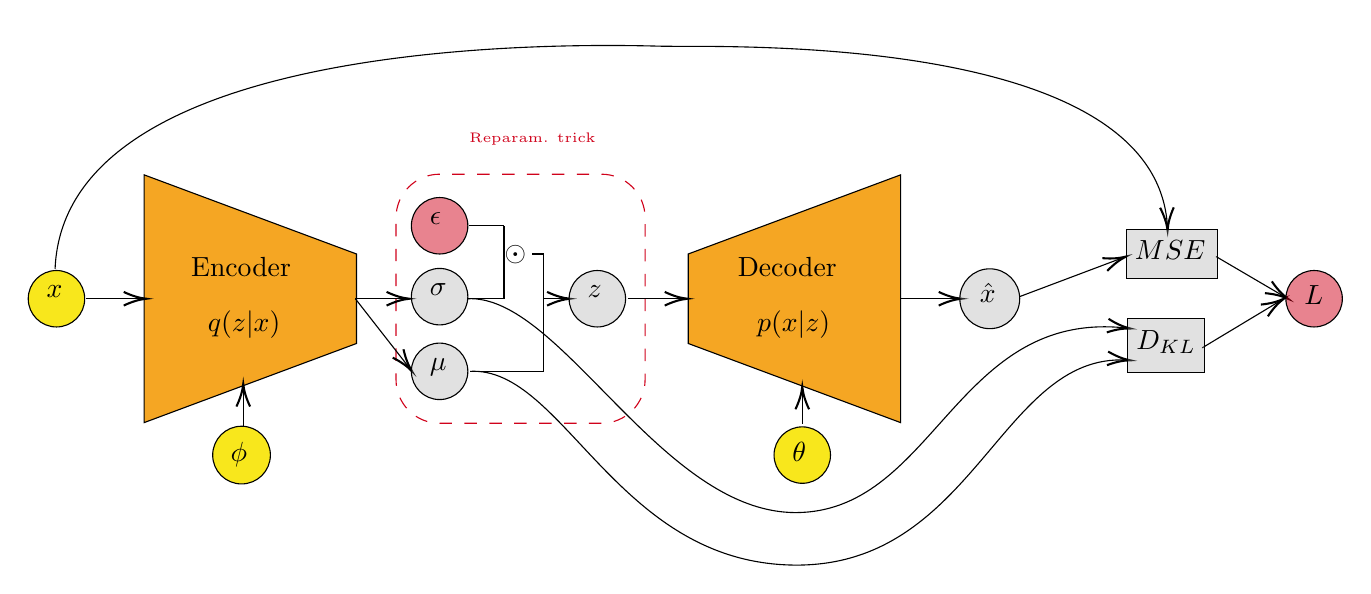
\begin{tikzpicture}[x=0.75pt,y=0.75pt,yscale=-1,xscale=1]
%uncomment if require: \path (0,300); %set diagram left start at 0, and has height of 300

%Shape: Trapezoid [id:dp7823603828525814] 
\draw  [fill={rgb, 255:red, 245; green, 166; blue, 35 }  ,fill opacity=1 ] (93.26,100.32) -- (195.56,138.44) -- (195.56,181.56) -- (93.26,219.68) -- cycle ;
%Flowchart: Alternative Process [id:dp7916519671015572] 
\draw  [color={rgb, 255:red, 208; green, 2; blue, 27 }  ,draw opacity=1 ][dash pattern={on 4.5pt off 4.5pt}] (313.6,100) .. controls (325.2,100) and (334.6,109.4) .. (334.6,121) -- (334.6,199) .. controls (334.6,210.6) and (325.2,220) .. (313.6,220) -- (235.6,220) .. controls (224,220) and (214.6,210.6) .. (214.6,199) -- (214.6,121) .. controls (214.6,109.4) and (224,100) .. (235.6,100) -- cycle ;
%Shape: Trapezoid [id:dp7878502215303758] 
\draw  [fill={rgb, 255:red, 245; green, 166; blue, 35 }  ,fill opacity=1 ] (457.69,219.68) -- (355.39,181.56) -- (355.39,138.44) -- (457.69,100.32) -- cycle ;
%Straight Lines [id:da7022493612643106] 
\draw    (65,160) -- (92.33,160) ;
\draw [shift={(94.33,160)}, rotate = 180] [color={rgb, 255:red, 0; green, 0; blue, 0 }  ][line width=0.75]    (10.93,-3.29) .. controls (6.95,-1.4) and (3.31,-0.3) .. (0,0) .. controls (3.31,0.3) and (6.95,1.4) .. (10.93,3.29)   ;
%Straight Lines [id:da842524726150703] 
\draw    (141,221.67) -- (141,203) ;
\draw [shift={(141,201)}, rotate = 90] [color={rgb, 255:red, 0; green, 0; blue, 0 }  ][line width=0.75]    (10.93,-3.29) .. controls (6.95,-1.4) and (3.31,-0.3) .. (0,0) .. controls (3.31,0.3) and (6.95,1.4) .. (10.93,3.29)   ;
%Straight Lines [id:da6004403121374124] 
\draw    (457.67,160) -- (485,160) ;
\draw [shift={(487,160)}, rotate = 180] [color={rgb, 255:red, 0; green, 0; blue, 0 }  ][line width=0.75]    (10.93,-3.29) .. controls (6.95,-1.4) and (3.31,-0.3) .. (0,0) .. controls (3.31,0.3) and (6.95,1.4) .. (10.93,3.29)   ;
%Straight Lines [id:da6888855782255758] 
\draw    (410.33,220.33) -- (410.33,204.33) ;
\draw [shift={(410.33,202.33)}, rotate = 90] [color={rgb, 255:red, 0; green, 0; blue, 0 }  ][line width=0.75]    (10.93,-3.29) .. controls (6.95,-1.4) and (3.31,-0.3) .. (0,0) .. controls (3.31,0.3) and (6.95,1.4) .. (10.93,3.29)   ;
%Straight Lines [id:da5580691014824746] 
\draw    (249.67,124.84) -- (266.6,124.84) ;
%Straight Lines [id:da0719604636131792] 
\draw    (249,160) -- (266.6,160) ;
%Straight Lines [id:da12715359384818892] 
\draw    (266.6,124.84) -- (266.6,160) ;
%Straight Lines [id:da1128909560545941] 
\draw    (285.67,194.98) -- (250.33,194.98) ;
%Straight Lines [id:da6821248002376252] 
\draw    (285.67,138.44) -- (285.67,194.98) ;
%Straight Lines [id:da18808034763917325] 
\draw    (280.33,138.44) -- (285.67,138.44) ;
%Straight Lines [id:da9818051915598998] 
\draw    (285.67,160) -- (296.33,160) ;
\draw [shift={(298.33,160)}, rotate = 180] [color={rgb, 255:red, 0; green, 0; blue, 0 }  ][line width=0.75]    (10.93,-3.29) .. controls (6.95,-1.4) and (3.31,-0.3) .. (0,0) .. controls (3.31,0.3) and (6.95,1.4) .. (10.93,3.29)   ;
%Straight Lines [id:da15034327030618333] 
\draw    (326.33,160) -- (353,160) ;
\draw [shift={(355,160)}, rotate = 180] [color={rgb, 255:red, 0; green, 0; blue, 0 }  ][line width=0.75]    (10.93,-3.29) .. controls (6.95,-1.4) and (3.31,-0.3) .. (0,0) .. controls (3.31,0.3) and (6.95,1.4) .. (10.93,3.29)   ;
%Straight Lines [id:da5118381101450515] 
\draw    (195,160) -- (219,160) ;
\draw [shift={(221,160)}, rotate = 180] [color={rgb, 255:red, 0; green, 0; blue, 0 }  ][line width=0.75]    (10.93,-3.29) .. controls (6.95,-1.4) and (3.31,-0.3) .. (0,0) .. controls (3.31,0.3) and (6.95,1.4) .. (10.93,3.29)   ;
%Straight Lines [id:da0008605514980692952] 
\draw    (195,160) -- (221.1,193.4) ;
\draw [shift={(222.33,194.98)}, rotate = 232] [color={rgb, 255:red, 0; green, 0; blue, 0 }  ][line width=0.75]    (10.93,-3.29) .. controls (6.95,-1.4) and (3.31,-0.3) .. (0,0) .. controls (3.31,0.3) and (6.95,1.4) .. (10.93,3.29)   ;
%Curve Lines [id:da606983672133339] 
\draw    (249,160) .. controls (294.33,157.67) and (343,265) .. (409,263) .. controls (474.67,261.01) and (484.9,164.64) .. (567.09,174.18) ;
\draw [shift={(568.33,174.33)}, rotate = 187.29] [color={rgb, 255:red, 0; green, 0; blue, 0 }  ][line width=0.75]    (10.93,-3.29) .. controls (6.95,-1.4) and (3.31,-0.3) .. (0,0) .. controls (3.31,0.3) and (6.95,1.4) .. (10.93,3.29)   ;
%Curve Lines [id:da10450467264141716] 
\draw    (250.33,194.98) .. controls (295.67,192.65) and (321,288.33) .. (407.67,288.33) .. controls (493.47,288.33) and (506.09,186.4) .. (566.49,189.54) ;
\draw [shift={(568.33,189.67)}, rotate = 184.92] [color={rgb, 255:red, 0; green, 0; blue, 0 }  ][line width=0.75]    (10.93,-3.29) .. controls (6.95,-1.4) and (3.31,-0.3) .. (0,0) .. controls (3.31,0.3) and (6.95,1.4) .. (10.93,3.29)   ;
%Curve Lines [id:da10659071061601377] 
\draw    (50.33,145.67) .. controls (55,29.67) and (314.33,37.67) .. (342.33,38.33) .. controls (370.19,39) and (581.54,31.08) .. (586.28,125.57) ;
\draw [shift={(586.33,127)}, rotate = 268.41] [color={rgb, 255:red, 0; green, 0; blue, 0 }  ][line width=0.75]    (10.93,-3.29) .. controls (6.95,-1.4) and (3.31,-0.3) .. (0,0) .. controls (3.31,0.3) and (6.95,1.4) .. (10.93,3.29)   ;
%Straight Lines [id:da6109248809176173] 
\draw    (515,159) -- (564.46,140.37) ;
\draw [shift={(566.33,139.67)}, rotate = 159.36] [color={rgb, 255:red, 0; green, 0; blue, 0 }  ][line width=0.75]    (10.93,-3.29) .. controls (6.95,-1.4) and (3.31,-0.3) .. (0,0) .. controls (3.31,0.3) and (6.95,1.4) .. (10.93,3.29)   ;
%Straight Lines [id:da2945225342159614] 
\draw    (609.67,139.67) -- (642.61,158.99) ;
\draw [shift={(644.33,160)}, rotate = 210.39] [color={rgb, 255:red, 0; green, 0; blue, 0 }  ][line width=0.75]    (10.93,-3.29) .. controls (6.95,-1.4) and (3.31,-0.3) .. (0,0) .. controls (3.31,0.3) and (6.95,1.4) .. (10.93,3.29)   ;
%Straight Lines [id:da8512352195616399] 
\draw    (603,183.67) -- (640.62,161.03) ;
\draw [shift={(642.33,160)}, rotate = 148.96] [color={rgb, 255:red, 0; green, 0; blue, 0 }  ][line width=0.75]    (10.93,-3.29) .. controls (6.95,-1.4) and (3.31,-0.3) .. (0,0) .. controls (3.31,0.3) and (6.95,1.4) .. (10.93,3.29)   ;

% Text Node
\draw  [fill={rgb, 255:red, 248; green, 231; blue, 28 }  ,fill opacity=1 ]  (51, 160) circle [x radius= 13.6, y radius= 13.6]   ;
\draw (45,152.4) node [anchor=north west][inner sep=0.75pt]    {$x$};
% Text Node
\draw (114.67,139) node [anchor=north west][inner sep=0.75pt]   [align=left] {Encoder};
% Text Node
\draw (122.67,164.4) node [anchor=north west][inner sep=0.75pt]    {$q( z|x)$};
% Text Node
\draw (378,139) node [anchor=north west][inner sep=0.75pt]   [align=left] {Decoder};
% Text Node
\draw (387.33,164.4) node [anchor=north west][inner sep=0.75pt]    {$p( x|z)$};
% Text Node
\draw  [fill={rgb, 255:red, 155; green, 155; blue, 155 }  ,fill opacity=0.3 ]  (500.67, 160) circle [x radius= 14.42, y radius= 14.42]   ;
\draw (494.67,151.4) node [anchor=north west][inner sep=0.75pt]    {$\hat{x}$};
% Text Node
\draw  [fill={rgb, 255:red, 248; green, 231; blue, 28 }  ,fill opacity=1 ]  (140.17, 235.33) circle [x radius= 13.9, y radius= 13.9]   ;
\draw (133.67,227.73) node [anchor=north west][inner sep=0.75pt]    {$\phi $};
% Text Node
\draw  [fill={rgb, 255:red, 208; green, 2; blue, 27 }  ,fill opacity=0.49 ]  (235.6, 124.84) circle [x radius= 13.6, y radius= 13.6]   ;
\draw (229.6,117.24) node [anchor=north west][inner sep=0.75pt]    {$\epsilon $};
% Text Node
\draw  [fill={rgb, 255:red, 248; green, 231; blue, 28 }  ,fill opacity=1 ]  (410.33, 235.33) circle [x radius= 13.6, y radius= 13.6]   ;
\draw (404.33,227.73) node [anchor=north west][inner sep=0.75pt]    {$\theta $};
% Text Node
\draw  [fill={rgb, 255:red, 155; green, 155; blue, 155 }  ,fill opacity=0.3 ]  (235.6, 159) circle [x radius= 13.6, y radius= 13.6]   ;
\draw (229.6,151.4) node [anchor=north west][inner sep=0.75pt]    {$\sigma $};
% Text Node
\draw  [fill={rgb, 255:red, 155; green, 155; blue, 155 }  ,fill opacity=0.3 ]  (235.6, 194.98) circle [x radius= 13.6, y radius= 13.6]   ;
\draw (229.6,187.38) node [anchor=north west][inner sep=0.75pt]    {$\mu $};
% Text Node
\draw  [fill={rgb, 255:red, 155; green, 155; blue, 155 }  ,fill opacity=0.3 ]  (311.6, 160) circle [x radius= 13.6, y radius= 13.6]   ;
\draw (305.6,152.4) node [anchor=north west][inner sep=0.75pt]    {$z$};
% Text Node
\draw (265.67,132.84) node [anchor=north west][inner sep=0.75pt]    {$\odot $};
% Text Node
\draw  [fill={rgb, 255:red, 155; green, 155; blue, 155 }  ,fill opacity=0.3 ]  (566.33,126.44) -- (610.33,126.44) -- (610.33,150.44) -- (566.33,150.44) -- cycle  ;
\draw (569.33,130.84) node [anchor=north west][inner sep=0.75pt]    {$MSE$};
% Text Node
\draw  [fill={rgb, 255:red, 155; green, 155; blue, 155 }  ,fill opacity=0.3 ]  (567,169.56) -- (604,169.56) -- (604,195.56) -- (567,195.56) -- cycle  ;
\draw (570,173.96) node [anchor=north west][inner sep=0.75pt]    {$D_{KL}$};
% Text Node
\draw (248.67,79) node [anchor=north west][inner sep=0.75pt]  [color={rgb, 255:red, 208; green, 2; blue, 27 }  ,opacity=1 ] [align=left] {{\tiny Reparam. trick}};
% Text Node
\draw  [fill={rgb, 255:red, 208; green, 2; blue, 27 }  ,fill opacity=0.49 ]  (656.93, 160) circle [x radius= 13.6, y radius= 13.6]   ;
\draw (650.93,152.4) node [anchor=north west][inner sep=0.75pt]    {$L$};


\end{tikzpicture}
    \caption[Architecture of Gaussian VAEs.]%
    { Architecture of Gaussian VAEs. The input $x$ is passed through the encoder with parameters $\phi$ producing the mean $\mu$ and the standard deviation $\sigma$ of the Gaussian distribution. The random variable $\epsilon$ is sampled from a standard Gaussian distribution and is used to sample $ z = \mu + \sigma \odot \epsilon$. The sampled $z$ is then passed through the decoder with parameters $\theta$ producing the output $\hat{x}$. The loss function to be minimized is the sum of the MSE reconstruction loss and the KL divergence regularization loss. 
    }
  	\medskip 
	\hspace*{15pt}\hbox{\scriptsize Credit: Adapted from Kingma and Welling~\cite{Kingma_2019} }\label{VAEFigure}
\end{figure}

\section{Vector Quantized VAEs}\label{background:vqvae}

Vector Quantized VAEs (VQ-VAEs) are a variant of VAEs that were introduced in 2017 by Aäron van den Oord et al.~\cite{vqvae}. The VQ-VAEs have shown various improvements over the standard VAEs, such as higher quality of the generated sampled, better disentanglement of the latent space and better generalization to unseen data. The VQ-VAEs have been used in various applications, such as image generation, speech synthesis and music generation, text to image generation~\cite{vqvae2,vqvaespeechsynthesis, musicvqvae,dalle}.

The VQVAEs fundamentally differs in two key ways from a VAEs. Firstly, the latent representation is discrete instead of continuous. Secondly, the prior distribution is learned rather than being fixed. The posterior and prior distributions are categorical and the samples taken from these distributions are the indices of the embeddings in the embedding space. These matched indices are then used to look up the embeddings in the embedding space and then used as input to the decoder~\cite{vqvae}. VQ-VAEs learning
process consists of two stages. In the first stage, the encoder and the decoder are trained. In the second stage prior over these discrete latent variables is trained~\cite{vqvae}.

\subsection{Discrete Latent Variables}

VQ-VAEs focus on discrete latent variables, which is a more natural fit for many types of data. Language and speech naturally is stream of discrete units, such as words or phonemes. Images can be often well described by language, which can the discrete representations well suited for images as well. Moreover, discrete representations work very well with complex reasoning, decision-making~\cite{vqvae}.

VQ-VAEs define a latent embedding space $ e \in \mathbb{R}^{K \times D} $, where $K$ is the number of embeddings and $D$ is the dimension of each latent embedding vector. The model takes an input $x$, which is passed through the encoder producing output $z_e(x)$, as shown in figure~\ref{VQVAEFigure}. 
The discrete latent variables $z$ are then calculated by nearest neighbor lookup in the embedding space
 \[ z = \argmin_{k} || z_e(x) - e_k ||^2,\] 
where $e_k$ is the $k$-th embedding vector in the embedding space. The decoder then takes the discrete latent variables $z$ and produces the output $\hat{x}$. 
One can see this forward propagation as a regular autoencoder with a quantization step in the middle~\cite{vqvae}.

The posterior categorical distribution $q_{\phi}(z|x)$ is defined as follows:
\begin{equation} \label{eqVQVAEPosterior}
    q(z=k|x) = \begin{cases}
        1& \text{if} \ k = \argmin_{k} || z_e(x) - e_k ||^2 \\
        0& \text{otherwise}
    \end{cases},
\end{equation}
where $z_e(x)$ is the output of the encoder network and $e_k$ is the $k$-th vector in the embedding table.
The discrete latent variable $z$ is then used to look up the corresponding embedding vector $e_k$ in the embedding space, which is then used as input to the decoder network. The decoder network then produces the output $\hat{x}$~\cite{vqvae}.
The decoder distribution $p_{\theta}(x|z)$ is assumed to be a Gaussian distribution.

\subsection{Learning}

As mentioned earlier, the VQ-VAEs introduce learning the prior distribution separately from the posterior distribution. The prior distribution is defined as a categorical distribution $p_{\omega}(z)$, where $z$ is a discrete latent variable~\cite{vqvae}.

Since the proposed posterior distribution $q_{\phi}(z|x)$ is a deterministic by applying it to ELBO objective, we get the following expression:
\begin{equation}
    \begin{split}
        L_{\theta, \phi, \omega}(x) &= - D_{KL}(q_{\phi}(z = k|x) || p_{\omega}(z)) + \mathbb{E}_{q_{\phi}(z=k|x)} [\log p_{\theta}(x|z = k)],\\
                            &= - \mathbb{E}_{q_{\phi}(z=k|x)} [\log \frac{q_{\phi}(z=k|x)}{p_{\omega}(z)}] + \mathbb{E}_{q_{\phi}(z=k|x)} [\log p_{\theta}(x|z = k)],\\
                            &= - \log \frac{1}{p_{\omega}(z)} + \log p_{\theta}(x|z = k),\\
                            &= \log p_{\omega}(z) + \log p_{\theta}(x|z = k),\\
    \end{split}
\end{equation}

The VQVAE learning process is then divided into two stages, where in the first stage the first term is ignored, and the second term is maximized. In the second stage, the prior distribution is trained. In the next 2 sections, I will describe both stages in more detail.

\subsubsection{First stage}

In the first stage the log likelihood of posterior distribution is \textbf{maximized}, which means the encoder and the decoder are trained with the prior distribution being arbitrary. The training objective in first stages reduces to 
\[ L_{\theta, \phi}(x) = \log p_{\theta}(x|z = k), \]
where $k$ is the index of the nearest embedding vector in the embedding space, which is defined in equation~\ref{eqVQVAEPosterior}. We can look at the first stage as training a regular autoencoder with a quantization step in the middle, which inherently makes the latent space distribution categorical~\cite{vqvae}.
    
However, the expression $k = \argmin_{k} || z_e(x) - e_k ||^2$ is not differentiable with respect to the parameters of the network. To make the training process differentiable, the authors of the VQ-VAEs propose to use the straight-through estimator, which is a way of estimating the gradients of the non-differentiable function, and copy the gradients of $z_q(x)$ to $z_e(x)$~\cite{vqvae}. The straight through estimator only works if the difference between $z_e(x)$ and $e_k$ is small, which can be achieved by adding extra loss terms to the training objective.~\cite{straight_through}

This is where the VQ objective comes in. The VQ objective uses the second term of equation~\ref{eqVQVAEObjective} to encourage the encoder to produce representations that are close to the embedding vectors in the embedding space, which is called the commitment loss~\cite{vqvae}.

However, since the embedding space can be arbitrary large the embedding vectors can be arbitrary far from the encoder output. To prevent this, the authors of the VQ-VAEs propose to add another term to the training objective, which is called the codebook loss. The codebook loss encourages the embedding vectors to be close to the encoder output. The codebook loss has $\beta$ as a hyperparameter, which controls the importance of the codebook loss~\cite{vqvae}.

Thus, the resulting training objective becomes
\begin{equation} \label{eqVQVAEObjective}
    \begin{split}
        L &= \log p_{\theta}(x|z = k) - \biggl( || sg(z_e(x)) - e_k ||^2 + \beta || z_q(x) - sg(e_k) ||^2 \biggr),\\
    \end{split}
\end{equation}
where $sg$ is the stop gradient operation, which is defined as identity function, but with the gradients of the output set to zero.

The loss function to be \textbf{minimized} for VQ-VAE's usually used in practice is the sum of the VQ objective and the MSE reconstruction loss.
The first term in the function is the MSE reconstruction loss because maximizing the Gaussian likelihood is approximately equivalent to minimizing the MSE reconstruction loss. This is shown in the equation~\ref{eqMSE}. 
Thus, the resulting training objective to be minimized becomes
\[ L = \frac{1}{D} \sum_{i=1}^{D} ||x_i - \hat{x}_i ||^2 + \frac{1}{Z} \sum_{i=1}^{Z} \biggl( || sg(z_e(x))_i - e_{k_{i}} ||^2 + \beta || z_q(x)_i -  sg(e_{k{i}}) ||^2 \biggr), \]
where $\hat{x} = f_{\theta}(z_q(x))$, where function $f_{\theta}$ is the decoder network, $D$ is the dimension of the input data, $Z$ is the number of latent space vectors and $k_{i}$ is the index of the nearest embedding vector in the embedding space for the $i$-th latent space vector, which is defined in equation~\ref{eqVQVAEPosterior}~\cite{vqvae}.

In the figure below~\ref{VQVAEFigure} there is a visualization of the architecture of VQ-VAEs.

\begin{figure}
    \centering 
    

\tikzset{every picture/.style={line width=0.75pt}} %set default line width to 0.75pt        

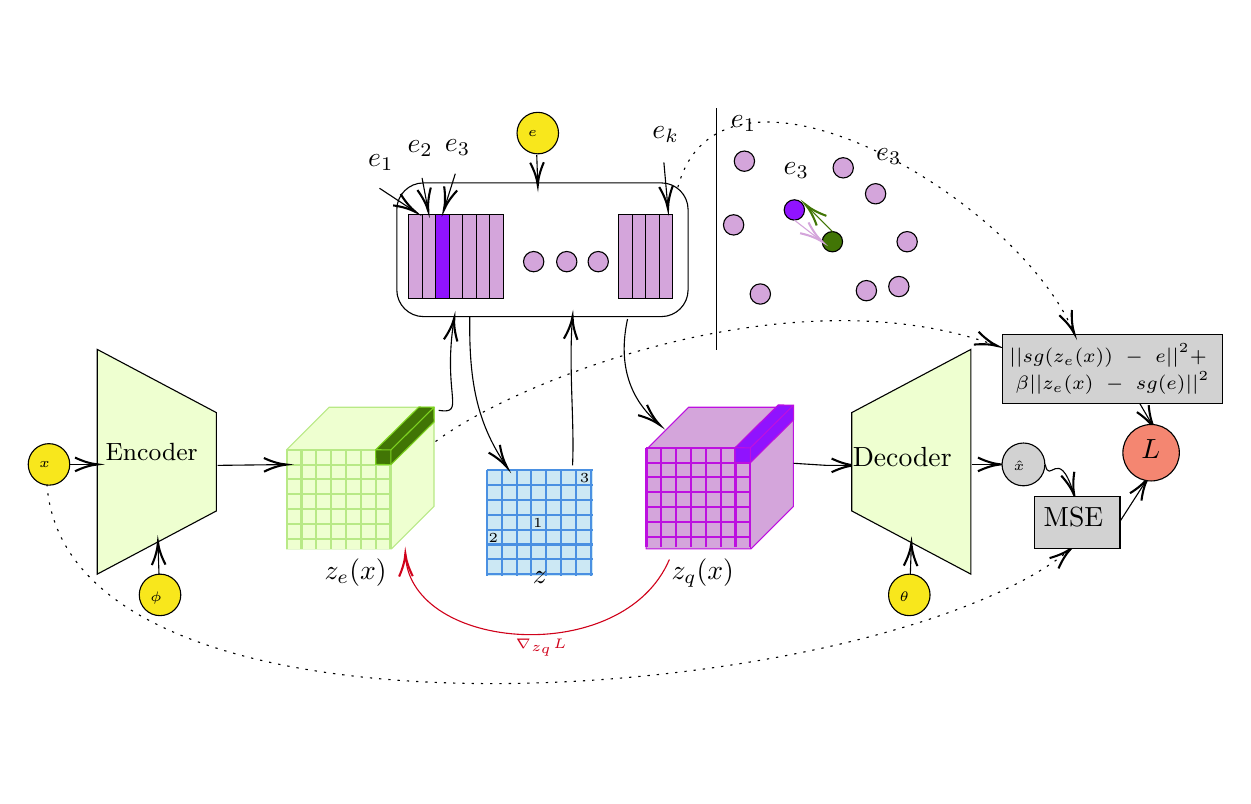
\begin{tikzpicture}[x=0.75pt,y=0.75pt,yscale=-1,xscale=1]
%uncomment if require: \path (0,308); %set diagram left start at 0, and has height of 308

%Shape: Trapezoid [id:dp36465646521888906] 
\draw  [fill={rgb, 255:red, 238; green, 255; blue, 208 }  ,fill opacity=1 ] (97.75,141.72) -- (155.17,172.18) -- (155.17,219.54) -- (97.75,250) -- cycle ;
%Shape: Cube [id:dp9839436955233336] 
\draw  [color={rgb, 255:red, 184; green, 233; blue, 134 }  ,draw opacity=1 ][fill={rgb, 255:red, 238; green, 255; blue, 208 }  ,fill opacity=1 ] (189,190.06) -- (209.47,169.59) -- (260,169.59) -- (260,217.36) -- (239.53,237.83) -- (189,237.83) -- cycle ; \draw  [color={rgb, 255:red, 184; green, 233; blue, 134 }  ,draw opacity=1 ] (260,169.59) -- (239.53,190.06) -- (189,190.06) ; \draw  [color={rgb, 255:red, 184; green, 233; blue, 134 }  ,draw opacity=1 ] (239.53,190.06) -- (239.53,237.83) ;
%Shape: Grid [id:dp5232564483036259] 
\draw  [draw opacity=0][fill={rgb, 255:red, 238; green, 255; blue, 208 }  ,fill opacity=1 ][line width=0.75]  (189,190.06) -- (239.36,190.06) -- (239.36,237.83) -- (189,237.83) -- cycle ; \draw  [color={rgb, 255:red, 184; green, 233; blue, 134 }  ,draw opacity=1 ][line width=0.75]  (189,190.06) -- (189,237.83)(196.15,190.06) -- (196.15,237.83)(203.3,190.06) -- (203.3,237.83)(210.45,190.06) -- (210.45,237.83)(217.6,190.06) -- (217.6,237.83)(224.75,190.06) -- (224.75,237.83)(231.9,190.06) -- (231.9,237.83)(239.05,190.06) -- (239.05,237.83) ; \draw  [color={rgb, 255:red, 184; green, 233; blue, 134 }  ,draw opacity=1 ][line width=0.75]  (189,190.06) -- (239.36,190.06)(189,197.21) -- (239.36,197.21)(189,204.36) -- (239.36,204.36)(189,211.51) -- (239.36,211.51)(189,218.66) -- (239.36,218.66)(189,225.81) -- (239.36,225.81)(189,232.96) -- (239.36,232.96) ; \draw  [color={rgb, 255:red, 184; green, 233; blue, 134 }  ,draw opacity=1 ][line width=0.75]   ;
%Shape: Cube [id:dp6386923890289404] 
\draw  [color={rgb, 255:red, 126; green, 211; blue, 33 }  ,draw opacity=1 ][fill={rgb, 255:red, 65; green, 117; blue, 5 }  ,fill opacity=1 ] (231.89,190.05) -- (252.68,169.48) -- (260,169.59) -- (260.03,176.67) -- (239.25,197.24) -- (231.92,197.13) -- cycle ; \draw  [color={rgb, 255:red, 126; green, 211; blue, 33 }  ,draw opacity=1 ] (260,169.59) -- (239.22,190.16) -- (231.89,190.05) ; \draw  [color={rgb, 255:red, 126; green, 211; blue, 33 }  ,draw opacity=1 ] (239.22,190.16) -- (239.25,197.24) ;
%Shape: Grid [id:dp2868467076547798] 
\draw  [draw opacity=0][fill={rgb, 255:red, 204; green, 232; blue, 244 }  ,fill opacity=1 ][line width=0.75]  (285.5,199.95) -- (336.5,199.95) -- (336.5,250.95) -- (285.5,250.95) -- cycle ; \draw  [color={rgb, 255:red, 74; green, 144; blue, 226 }  ,draw opacity=1 ][line width=0.75]  (285.5,199.95) -- (285.5,250.95)(292.65,199.95) -- (292.65,250.95)(299.8,199.95) -- (299.8,250.95)(306.95,199.95) -- (306.95,250.95)(314.1,199.95) -- (314.1,250.95)(321.25,199.95) -- (321.25,250.95)(328.4,199.95) -- (328.4,250.95)(335.55,199.95) -- (335.55,250.95) ; \draw  [color={rgb, 255:red, 74; green, 144; blue, 226 }  ,draw opacity=1 ][line width=0.75]  (285.5,199.95) -- (336.5,199.95)(285.5,207.1) -- (336.5,207.1)(285.5,214.25) -- (336.5,214.25)(285.5,221.4) -- (336.5,221.4)(285.5,228.55) -- (336.5,228.55)(285.5,235.7) -- (336.5,235.7)(285.5,242.85) -- (336.5,242.85)(285.5,250) -- (336.5,250) ; \draw  [color={rgb, 255:red, 74; green, 144; blue, 226 }  ,draw opacity=1 ][line width=0.75]   ;
%Shape: Cube [id:dp9385697445458008] 
\draw  [color={rgb, 255:red, 189; green, 16; blue, 224 }  ,draw opacity=1 ][fill={rgb, 255:red, 212; green, 165; blue, 219 }  ,fill opacity=1 ] (362.17,190.06) -- (382.64,169.59) -- (433.17,169.59) -- (433.17,217.36) -- (412.69,237.83) -- (362.17,237.83) -- cycle ; \draw  [color={rgb, 255:red, 189; green, 16; blue, 224 }  ,draw opacity=1 ] (433.17,169.59) -- (412.69,190.06) -- (362.17,190.06) ; \draw  [color={rgb, 255:red, 189; green, 16; blue, 224 }  ,draw opacity=1 ] (412.69,190.06) -- (412.69,237.83) ;
%Shape: Grid [id:dp22814793354422447] 
\draw  [draw opacity=0][fill={rgb, 255:red, 212; green, 165; blue, 219 }  ,fill opacity=1 ][line width=0.75]  (362.37,189.11) -- (412.73,189.11) -- (412.73,236.88) -- (362.37,236.88) -- cycle ; \draw  [color={rgb, 255:red, 189; green, 16; blue, 224 }  ,draw opacity=1 ][line width=0.75]  (362.37,189.11) -- (362.37,236.88)(369.52,189.11) -- (369.52,236.88)(376.67,189.11) -- (376.67,236.88)(383.82,189.11) -- (383.82,236.88)(390.97,189.11) -- (390.97,236.88)(398.12,189.11) -- (398.12,236.88)(405.27,189.11) -- (405.27,236.88)(412.42,189.11) -- (412.42,236.88) ; \draw  [color={rgb, 255:red, 189; green, 16; blue, 224 }  ,draw opacity=1 ][line width=0.75]  (362.37,189.11) -- (412.73,189.11)(362.37,196.26) -- (412.73,196.26)(362.37,203.41) -- (412.73,203.41)(362.37,210.56) -- (412.73,210.56)(362.37,217.71) -- (412.73,217.71)(362.37,224.86) -- (412.73,224.86)(362.37,232.01) -- (412.73,232.01) ; \draw  [color={rgb, 255:red, 189; green, 16; blue, 224 }  ,draw opacity=1 ][line width=0.75]   ;
%Rounded Rect [id:dp987340568559665] 
\draw   (242.08,74.38) .. controls (242.08,67.27) and (247.85,61.5) .. (254.97,61.5) -- (369.53,61.5) .. controls (376.65,61.5) and (382.42,67.27) .. (382.42,74.38) -- (382.42,113.03) .. controls (382.42,120.15) and (376.65,125.92) .. (369.53,125.92) -- (254.97,125.92) .. controls (247.85,125.92) and (242.08,120.15) .. (242.08,113.03) -- cycle ;
%Shape: Rectangle [id:dp30823863628595904] 
\draw  [fill={rgb, 255:red, 212; green, 165; blue, 219 }  ,fill opacity=1 ] (247.83,76.83) -- (254.33,76.83) -- (254.33,117) -- (247.83,117) -- cycle ;
%Shape: Rectangle [id:dp5997971655975829] 
\draw  [fill={rgb, 255:red, 212; green, 165; blue, 219 }  ,fill opacity=1 ] (254.33,76.83) -- (260.83,76.83) -- (260.83,117) -- (254.33,117) -- cycle ;
%Shape: Rectangle [id:dp9067829242009235] 
\draw  [fill={rgb, 255:red, 144; green, 19; blue, 254 }  ,fill opacity=1 ] (260.83,76.83) -- (267.33,76.83) -- (267.33,117) -- (260.83,117) -- cycle ;
%Shape: Rectangle [id:dp9839671090206037] 
\draw  [fill={rgb, 255:red, 212; green, 165; blue, 219 }  ,fill opacity=1 ] (267.33,76.83) -- (273.83,76.83) -- (273.83,117) -- (267.33,117) -- cycle ;
%Shape: Rectangle [id:dp637271918983642] 
\draw  [fill={rgb, 255:red, 212; green, 165; blue, 219 }  ,fill opacity=1 ] (273.83,76.83) -- (280.33,76.83) -- (280.33,117) -- (273.83,117) -- cycle ;
%Shape: Rectangle [id:dp6037901670914401] 
\draw  [fill={rgb, 255:red, 212; green, 165; blue, 219 }  ,fill opacity=1 ] (280.33,76.83) -- (286.83,76.83) -- (286.83,117) -- (280.33,117) -- cycle ;
%Shape: Rectangle [id:dp5095550610243931] 
\draw  [fill={rgb, 255:red, 212; green, 165; blue, 219 }  ,fill opacity=1 ] (286.83,76.83) -- (293.33,76.83) -- (293.33,117) -- (286.83,117) -- cycle ;
%Shape: Rectangle [id:dp567247771177326] 
\draw  [fill={rgb, 255:red, 212; green, 165; blue, 219 }  ,fill opacity=1 ] (349,76.83) -- (355.5,76.83) -- (355.5,117) -- (349,117) -- cycle ;
%Shape: Rectangle [id:dp845410248827495] 
\draw  [fill={rgb, 255:red, 212; green, 165; blue, 219 }  ,fill opacity=1 ] (355.5,76.83) -- (362,76.83) -- (362,117) -- (355.5,117) -- cycle ;
%Shape: Rectangle [id:dp6861462857716385] 
\draw  [fill={rgb, 255:red, 212; green, 165; blue, 219 }  ,fill opacity=1 ] (362,76.83) -- (368.5,76.83) -- (368.5,117) -- (362,117) -- cycle ;
%Shape: Rectangle [id:dp4814994913911068] 
\draw  [fill={rgb, 255:red, 212; green, 165; blue, 219 }  ,fill opacity=1 ] (368.5,76.83) -- (375,76.83) -- (375,117) -- (368.5,117) -- cycle ;
%Shape: Circle [id:dp522837592365686] 
\draw  [fill={rgb, 255:red, 212; green, 165; blue, 219 }  ,fill opacity=1 ] (319.06,99.44) .. controls (319.06,96.73) and (321.25,94.54) .. (323.96,94.54) .. controls (326.66,94.54) and (328.85,96.73) .. (328.85,99.44) .. controls (328.85,102.14) and (326.66,104.33) .. (323.96,104.33) .. controls (321.25,104.33) and (319.06,102.14) .. (319.06,99.44) -- cycle ;
%Shape: Circle [id:dp6306767856366036] 
\draw  [fill={rgb, 255:red, 212; green, 165; blue, 219 }  ,fill opacity=1 ] (334.23,99.44) .. controls (334.23,96.73) and (336.42,94.54) .. (339.12,94.54) .. controls (341.83,94.54) and (344.02,96.73) .. (344.02,99.44) .. controls (344.02,102.14) and (341.83,104.33) .. (339.12,104.33) .. controls (336.42,104.33) and (334.23,102.14) .. (334.23,99.44) -- cycle ;
%Shape: Circle [id:dp21003947259846445] 
\draw  [fill={rgb, 255:red, 212; green, 165; blue, 219 }  ,fill opacity=1 ] (303.12,99.44) .. controls (303.12,96.73) and (305.31,94.54) .. (308.02,94.54) .. controls (310.72,94.54) and (312.92,96.73) .. (312.92,99.44) .. controls (312.92,102.14) and (310.72,104.33) .. (308.02,104.33) .. controls (305.31,104.33) and (303.12,102.14) .. (303.12,99.44) -- cycle ;
%Straight Lines [id:da4730245477119335] 
\draw    (233.75,64.09) -- (249.58,74.49) ;
\draw [shift={(251.25,75.59)}, rotate = 213.31] [color={rgb, 255:red, 0; green, 0; blue, 0 }  ][line width=0.75]    (10.93,-3.29) .. controls (6.95,-1.4) and (3.31,-0.3) .. (0,0) .. controls (3.31,0.3) and (6.95,1.4) .. (10.93,3.29)   ;
%Straight Lines [id:da7768631230213965] 
\draw    (254.25,59.09) -- (256.88,73.12) ;
\draw [shift={(257.25,75.09)}, rotate = 259.38] [color={rgb, 255:red, 0; green, 0; blue, 0 }  ][line width=0.75]    (10.93,-3.29) .. controls (6.95,-1.4) and (3.31,-0.3) .. (0,0) .. controls (3.31,0.3) and (6.95,1.4) .. (10.93,3.29)   ;
%Straight Lines [id:da9227058463688853] 
\draw    (270.25,57.09) -- (265.35,72.68) ;
\draw [shift={(264.75,74.59)}, rotate = 287.45] [color={rgb, 255:red, 0; green, 0; blue, 0 }  ][line width=0.75]    (10.93,-3.29) .. controls (6.95,-1.4) and (3.31,-0.3) .. (0,0) .. controls (3.31,0.3) and (6.95,1.4) .. (10.93,3.29)   ;
%Straight Lines [id:da5035350182337077] 
\draw    (370.75,51.59) -- (372.57,72.09) ;
\draw [shift={(372.75,74.09)}, rotate = 264.92] [color={rgb, 255:red, 0; green, 0; blue, 0 }  ][line width=0.75]    (10.93,-3.29) .. controls (6.95,-1.4) and (3.31,-0.3) .. (0,0) .. controls (3.31,0.3) and (6.95,1.4) .. (10.93,3.29)   ;
%Shape: Cube [id:dp5455643438926754] 
\draw  [color={rgb, 255:red, 189; green, 16; blue, 224 }  ,draw opacity=1 ][fill={rgb, 255:red, 144; green, 19; blue, 254 }  ,fill opacity=1 ] (405.07,189.06) -- (425.85,168.49) -- (433.18,168.6) -- (433.21,175.69) -- (412.42,196.26) -- (405.1,196.15) -- cycle ; \draw  [color={rgb, 255:red, 189; green, 16; blue, 224 }  ,draw opacity=1 ] (433.18,168.6) -- (412.39,189.17) -- (405.07,189.06) ; \draw  [color={rgb, 255:red, 189; green, 16; blue, 224 }  ,draw opacity=1 ] (412.39,189.17) -- (412.42,196.26) ;
%Straight Lines [id:da0934101569879584] 
\draw    (433.25,196.59) -- (449,197.59) -- (460.5,197.59) ;
\draw [shift={(462.5,197.59)}, rotate = 180] [color={rgb, 255:red, 0; green, 0; blue, 0 }  ][line width=0.75]    (10.93,-3.29) .. controls (6.95,-1.4) and (3.31,-0.3) .. (0,0) .. controls (3.31,0.3) and (6.95,1.4) .. (10.93,3.29)   ;
%Straight Lines [id:da9792182129604674] 
\draw    (155.75,197.59) -- (187,197.23) ;
\draw [shift={(189,197.21)}, rotate = 179.35] [color={rgb, 255:red, 0; green, 0; blue, 0 }  ][line width=0.75]    (10.93,-3.29) .. controls (6.95,-1.4) and (3.31,-0.3) .. (0,0) .. controls (3.31,0.3) and (6.95,1.4) .. (10.93,3.29)   ;
%Curve Lines [id:da2262261338808227] 
\draw    (277.25,125.92) .. controls (276.76,156.63) and (280.55,176.57) .. (294.18,197.01) ;
\draw [shift={(295.25,198.59)}, rotate = 235.38] [color={rgb, 255:red, 0; green, 0; blue, 0 }  ][line width=0.75]    (10.93,-3.29) .. controls (6.95,-1.4) and (3.31,-0.3) .. (0,0) .. controls (3.31,0.3) and (6.95,1.4) .. (10.93,3.29)   ;
%Curve Lines [id:da9241998830342757] 
\draw    (262.25,171.09) .. controls (275.55,173.06) and (264.1,164.35) .. (269.49,128.25) ;
\draw [shift={(269.75,126.59)}, rotate = 99.09] [color={rgb, 255:red, 0; green, 0; blue, 0 }  ][line width=0.75]    (10.93,-3.29) .. controls (6.95,-1.4) and (3.31,-0.3) .. (0,0) .. controls (3.31,0.3) and (6.95,1.4) .. (10.93,3.29)   ;
%Curve Lines [id:da3327456466588097] 
\draw    (326.75,197.59) .. controls (327.73,177.11) and (324.9,151.72) .. (326.61,127.76) ;
\draw [shift={(326.75,125.92)}, rotate = 94.67] [color={rgb, 255:red, 0; green, 0; blue, 0 }  ][line width=0.75]    (10.93,-3.29) .. controls (6.95,-1.4) and (3.31,-0.3) .. (0,0) .. controls (3.31,0.3) and (6.95,1.4) .. (10.93,3.29)   ;
%Curve Lines [id:da9765543501242715] 
\draw    (353.25,127.09) .. controls (347.14,155.29) and (359.59,169.79) .. (367.33,176.83) ;
\draw [shift={(368.75,178.09)}, rotate = 220.91] [color={rgb, 255:red, 0; green, 0; blue, 0 }  ][line width=0.75]    (10.93,-3.29) .. controls (6.95,-1.4) and (3.31,-0.3) .. (0,0) .. controls (3.31,0.3) and (6.95,1.4) .. (10.93,3.29)   ;
%Shape: Trapezoid [id:dp8428747340164717] 
\draw  [fill={rgb, 255:red, 238; green, 255; blue, 208 }  ,fill opacity=1 ] (518.67,250) -- (461.25,219.54) -- (461.25,172.18) -- (518.67,141.72) -- cycle ;
%Straight Lines [id:da3079769057377866] 
\draw    (396.25,25.59) -- (396.25,142.09) ;
%Shape: Circle [id:dp9948358303216249] 
\draw  [fill={rgb, 255:red, 144; green, 19; blue, 254 }  ,fill opacity=1 ] (428.72,74.53) .. controls (428.72,71.83) and (430.91,69.63) .. (433.62,69.63) .. controls (436.32,69.63) and (438.52,71.83) .. (438.52,74.53) .. controls (438.52,77.24) and (436.32,79.43) .. (433.62,79.43) .. controls (430.91,79.43) and (428.72,77.24) .. (428.72,74.53) -- cycle ;
%Shape: Circle [id:dp5522117322076687] 
\draw  [fill={rgb, 255:red, 212; green, 165; blue, 219 }  ,fill opacity=1 ] (412.32,115.04) .. controls (412.32,112.33) and (414.51,110.14) .. (417.22,110.14) .. controls (419.92,110.14) and (422.12,112.33) .. (422.12,115.04) .. controls (422.12,117.74) and (419.92,119.93) .. (417.22,119.93) .. controls (414.51,119.93) and (412.32,117.74) .. (412.32,115.04) -- cycle ;
%Shape: Circle [id:dp37361306443013786] 
\draw  [fill={rgb, 255:red, 212; green, 165; blue, 219 }  ,fill opacity=1 ] (463.43,113.42) .. controls (463.43,110.71) and (465.62,108.52) .. (468.32,108.52) .. controls (471.03,108.52) and (473.22,110.71) .. (473.22,113.42) .. controls (473.22,116.12) and (471.03,118.32) .. (468.32,118.32) .. controls (465.62,118.32) and (463.43,116.12) .. (463.43,113.42) -- cycle ;
%Shape: Circle [id:dp891940541408015] 
\draw  [fill={rgb, 255:red, 212; green, 165; blue, 219 }  ,fill opacity=1 ] (399.46,81.73) .. controls (399.46,79.03) and (401.65,76.83) .. (404.36,76.83) .. controls (407.06,76.83) and (409.25,79.03) .. (409.25,81.73) .. controls (409.25,84.44) and (407.06,86.63) .. (404.36,86.63) .. controls (401.65,86.63) and (399.46,84.44) .. (399.46,81.73) -- cycle ;
%Shape: Circle [id:dp2010992949282573] 
\draw  [fill={rgb, 255:red, 65; green, 117; blue, 5 }  ,fill opacity=1 ] (447.06,89.84) .. controls (447.06,87.13) and (449.25,84.94) .. (451.96,84.94) .. controls (454.66,84.94) and (456.85,87.13) .. (456.85,89.84) .. controls (456.85,92.54) and (454.66,94.73) .. (451.96,94.73) .. controls (449.25,94.73) and (447.06,92.54) .. (447.06,89.84) -- cycle ;
%Shape: Circle [id:dp6580309194400682] 
\draw  [fill={rgb, 255:red, 212; green, 165; blue, 219 }  ,fill opacity=1 ] (452.26,54.24) .. controls (452.26,51.53) and (454.45,49.34) .. (457.16,49.34) .. controls (459.86,49.34) and (462.05,51.53) .. (462.05,54.24) .. controls (462.05,56.94) and (459.86,59.13) .. (457.16,59.13) .. controls (454.45,59.13) and (452.26,56.94) .. (452.26,54.24) -- cycle ;
%Shape: Circle [id:dp3786180692063268] 
\draw  [fill={rgb, 255:red, 212; green, 165; blue, 219 }  ,fill opacity=1 ] (467.86,66.74) .. controls (467.86,64.03) and (470.05,61.84) .. (472.76,61.84) .. controls (475.46,61.84) and (477.65,64.03) .. (477.65,66.74) .. controls (477.65,69.44) and (475.46,71.63) .. (472.76,71.63) .. controls (470.05,71.63) and (467.86,69.44) .. (467.86,66.74) -- cycle ;
%Shape: Circle [id:dp5880744034956527] 
\draw  [fill={rgb, 255:red, 212; green, 165; blue, 219 }  ,fill opacity=1 ] (483.06,89.84) .. controls (483.06,87.13) and (485.25,84.94) .. (487.96,84.94) .. controls (490.66,84.94) and (492.85,87.13) .. (492.85,89.84) .. controls (492.85,92.54) and (490.66,94.73) .. (487.96,94.73) .. controls (485.25,94.73) and (483.06,92.54) .. (483.06,89.84) -- cycle ;
%Shape: Circle [id:dp7728747717342119] 
\draw  [fill={rgb, 255:red, 212; green, 165; blue, 219 }  ,fill opacity=1 ] (479.06,111.44) .. controls (479.06,108.73) and (481.25,106.54) .. (483.96,106.54) .. controls (486.66,106.54) and (488.85,108.73) .. (488.85,111.44) .. controls (488.85,114.14) and (486.66,116.33) .. (483.96,116.33) .. controls (481.25,116.33) and (479.06,114.14) .. (479.06,111.44) -- cycle ;
%Shape: Circle [id:dp8092299894843566] 
\draw  [fill={rgb, 255:red, 212; green, 165; blue, 219 }  ,fill opacity=1 ] (404.66,51.04) .. controls (404.66,48.33) and (406.85,46.14) .. (409.56,46.14) .. controls (412.26,46.14) and (414.45,48.33) .. (414.45,51.04) .. controls (414.45,53.74) and (412.26,55.93) .. (409.56,55.93) .. controls (406.85,55.93) and (404.66,53.74) .. (404.66,51.04) -- cycle ;
%Straight Lines [id:da48440557106316784] 
\draw [color={rgb, 255:red, 212; green, 165; blue, 219 }  ,draw opacity=1 ]   (433.62,79.43) -- (445.48,88.61) ;
\draw [shift={(447.06,89.84)}, rotate = 217.76] [color={rgb, 255:red, 212; green, 165; blue, 219 }  ,draw opacity=1 ][line width=0.75]    (10.93,-3.29) .. controls (6.95,-1.4) and (3.31,-0.3) .. (0,0) .. controls (3.31,0.3) and (6.95,1.4) .. (10.93,3.29)   ;
%Straight Lines [id:da1905841532534014] 
\draw [color={rgb, 255:red, 65; green, 117; blue, 5 }  ,draw opacity=1 ][fill={rgb, 255:red, 65; green, 117; blue, 5 }  ,fill opacity=1 ]   (451.96,84.94) -- (440.41,73.35) ;
\draw [shift={(439,71.94)}, rotate = 45.1] [color={rgb, 255:red, 65; green, 117; blue, 5 }  ,draw opacity=1 ][line width=0.75]    (10.93,-3.29) .. controls (6.95,-1.4) and (3.31,-0.3) .. (0,0) .. controls (3.31,0.3) and (6.95,1.4) .. (10.93,3.29)   ;
%Straight Lines [id:da3646207939780566] 
\draw    (84.5,197.13) -- (96,197.13) ;
\draw [shift={(98,197.13)}, rotate = 180] [color={rgb, 255:red, 0; green, 0; blue, 0 }  ][line width=0.75]    (10.93,-3.29) .. controls (6.95,-1.4) and (3.31,-0.3) .. (0,0) .. controls (3.31,0.3) and (6.95,1.4) .. (10.93,3.29)   ;
%Straight Lines [id:da7414471835536174] 
\draw    (127.5,250) -- (127.06,236.59) ;
\draw [shift={(127,234.59)}, rotate = 88.14] [color={rgb, 255:red, 0; green, 0; blue, 0 }  ][line width=0.75]    (10.93,-3.29) .. controls (6.95,-1.4) and (3.31,-0.3) .. (0,0) .. controls (3.31,0.3) and (6.95,1.4) .. (10.93,3.29)   ;
%Straight Lines [id:da6532112868086741] 
\draw    (489.5,250) -- (489.93,237.09) ;
\draw [shift={(490,235.09)}, rotate = 91.92] [color={rgb, 255:red, 0; green, 0; blue, 0 }  ][line width=0.75]    (10.93,-3.29) .. controls (6.95,-1.4) and (3.31,-0.3) .. (0,0) .. controls (3.31,0.3) and (6.95,1.4) .. (10.93,3.29)   ;
%Straight Lines [id:da567944360754334] 
\draw    (309.5,48.09) -- (309.93,60.59) ;
\draw [shift={(310,62.59)}, rotate = 268.03] [color={rgb, 255:red, 0; green, 0; blue, 0 }  ][line width=0.75]    (10.93,-3.29) .. controls (6.95,-1.4) and (3.31,-0.3) .. (0,0) .. controls (3.31,0.3) and (6.95,1.4) .. (10.93,3.29)   ;
%Straight Lines [id:da5426639611340927] 
\draw    (519,197.13) -- (531,197.13) ;
\draw [shift={(533,197.13)}, rotate = 180] [color={rgb, 255:red, 0; green, 0; blue, 0 }  ][line width=0.75]    (10.93,-3.29) .. controls (6.95,-1.4) and (3.31,-0.3) .. (0,0) .. controls (3.31,0.3) and (6.95,1.4) .. (10.93,3.29)   ;
%Curve Lines [id:da3458703024373422] 
\draw  [dash pattern={on 0.84pt off 2.51pt}]  (73.5,206.59) .. controls (83.45,346.89) and (477.53,311.95) .. (565.69,238.7) ;
\draw [shift={(567,237.59)}, rotate = 139.12] [color={rgb, 255:red, 0; green, 0; blue, 0 }  ][line width=0.75]    (10.93,-3.29) .. controls (6.95,-1.4) and (3.31,-0.3) .. (0,0) .. controls (3.31,0.3) and (6.95,1.4) .. (10.93,3.29)   ;
%Curve Lines [id:da6339473919323386] 
\draw  [dash pattern={on 0.84pt off 2.51pt}]  (260.75,186.09) .. controls (300.55,156.24) and (432.17,104.61) .. (530.03,139.56) ;
\draw [shift={(531.5,140.09)}, rotate = 200.17] [color={rgb, 255:red, 0; green, 0; blue, 0 }  ][line width=0.75]    (10.93,-3.29) .. controls (6.95,-1.4) and (3.31,-0.3) .. (0,0) .. controls (3.31,0.3) and (6.95,1.4) .. (10.93,3.29)   ;
%Curve Lines [id:da9053875872036645] 
\draw    (554.5,197.13) .. controls (556.45,207.33) and (560.78,188.1) .. (567.94,210.3) ;
\draw [shift={(568.5,212.09)}, rotate = 253.3] [color={rgb, 255:red, 0; green, 0; blue, 0 }  ][line width=0.75]    (10.93,-3.29) .. controls (6.95,-1.4) and (3.31,-0.3) .. (0,0) .. controls (3.31,0.3) and (6.95,1.4) .. (10.93,3.29)   ;
%Straight Lines [id:da6669066474499481] 
\draw    (590.5,224.59) -- (602.92,205.28) ;
\draw [shift={(604,203.59)}, rotate = 122.74] [color={rgb, 255:red, 0; green, 0; blue, 0 }  ][line width=0.75]    (10.93,-3.29) .. controls (6.95,-1.4) and (3.31,-0.3) .. (0,0) .. controls (3.31,0.3) and (6.95,1.4) .. (10.93,3.29)   ;
%Shape: Rectangle [id:dp9130971852580467] 
\draw  [fill={rgb, 255:red, 210; green, 210; blue, 210 }  ,fill opacity=1 ] (534,134.71) -- (640,134.71) -- (640,167.71) -- (534,167.71) -- cycle ;
%Straight Lines [id:da6493785264569487] 
\draw    (600,167.71) -- (605.99,177.98) ;
\draw [shift={(607,179.71)}, rotate = 239.74] [color={rgb, 255:red, 0; green, 0; blue, 0 }  ][line width=0.75]    (10.93,-3.29) .. controls (6.95,-1.4) and (3.31,-0.3) .. (0,0) .. controls (3.31,0.3) and (6.95,1.4) .. (10.93,3.29)   ;
%Curve Lines [id:da9064943672927692] 
\draw  [dash pattern={on 0.84pt off 2.51pt}]  (377.5,63.59) .. controls (397.9,-13.02) and (539.08,66.29) .. (568.07,133.09) ;
\draw [shift={(568.5,134.09)}, rotate = 247.32] [color={rgb, 255:red, 0; green, 0; blue, 0 }  ][line width=0.75]    (10.93,-3.29) .. controls (6.95,-1.4) and (3.31,-0.3) .. (0,0) .. controls (3.31,0.3) and (6.95,1.4) .. (10.93,3.29)   ;
%Curve Lines [id:da5299666678217625] 
\draw [color={rgb, 255:red, 208; green, 2; blue, 27 }  ,draw opacity=1 ]   (373.4,242.94) .. controls (351.22,295.22) and (249.46,287.51) .. (246.27,241.55) ;
\draw [shift={(246.2,240.14)}, rotate = 88.54] [color={rgb, 255:red, 208; green, 2; blue, 27 }  ,draw opacity=1 ][line width=0.75]    (10.93,-3.29) .. controls (6.95,-1.4) and (3.31,-0.3) .. (0,0) .. controls (3.31,0.3) and (6.95,1.4) .. (10.93,3.29)   ;

% Text Node
\draw (206,241.4) node [anchor=north west][inner sep=0.75pt]    {$z_{e}( x)$};
% Text Node
\draw (373.17,241.4) node [anchor=north west][inner sep=0.75pt]    {$z_{q}( x)$};
% Text Node
\draw (227,46.4) node [anchor=north west][inner sep=0.75pt]    {$e_{1}$};
% Text Node
\draw (246,39.9) node [anchor=north west][inner sep=0.75pt]    {$e_{2}$};
% Text Node
\draw (264,39.4) node [anchor=north west][inner sep=0.75pt]    {$e_{3}$};
% Text Node
\draw (364,32.9) node [anchor=north west][inner sep=0.75pt]    {$e_{k}$};
% Text Node
\draw (329,200.4) node [anchor=north west][inner sep=0.75pt]  [font=\tiny]  {$3$};
% Text Node
\draw (100.5,185.5) node [anchor=north west][inner sep=0.75pt]   [align=left] {{\small Encoder}};
% Text Node
\draw (460.5,187.5) node [anchor=north west][inner sep=0.75pt]   [align=left] {Decoder};
% Text Node
\draw (427.2,50.4) node [anchor=north west][inner sep=0.75pt]   [align=left] {$\displaystyle e_{3}$};
% Text Node
\draw (401.8,27.6) node [anchor=north west][inner sep=0.75pt]    {$e_{1}$};
% Text Node
\draw (471.8,43.6) node [anchor=north west][inner sep=0.75pt]    {$e_{3}$};
% Text Node
\draw  [fill={rgb, 255:red, 248; green, 231; blue, 28 }  ,fill opacity=1 ]  (128, 260) circle [x radius= 10, y radius= 10]   ;
\draw (122,257.4) node [anchor=north west][inner sep=0.75pt]  [font=\tiny]  {$\phi $};
% Text Node
\draw  [fill={rgb, 255:red, 248; green, 231; blue, 28 }  ,fill opacity=1 ]  (489, 260) circle [x radius= 10, y radius= 10]   ;
\draw (483,257.4) node [anchor=north west][inner sep=0.75pt]  [font=\tiny]  {$\theta $};
% Text Node
\draw  [fill={rgb, 255:red, 248; green, 231; blue, 28 }  ,fill opacity=1 ]  (74.5, 197.13) circle [x radius= 10, y radius= 10]   ;
\draw (68.5,194.53) node [anchor=north west][inner sep=0.75pt]  [font=\tiny]  {$x$};
% Text Node
\draw  [fill={rgb, 255:red, 210; green, 210; blue, 210 }  ,fill opacity=1 ]  (544, 197.13) circle [x radius= 10.31, y radius= 10.31]   ;
\draw (538,194.03) node [anchor=north west][inner sep=0.75pt]  [font=\tiny]  {$\hat{x}$};
% Text Node
\draw  [fill={rgb, 255:red, 248; green, 231; blue, 28 }  ,fill opacity=1 ]  (310, 37.5) circle [x radius= 10, y radius= 10]   ;
\draw (304,34.9) node [anchor=north west][inner sep=0.75pt]  [font=\tiny]  {$e$};
% Text Node
\draw  [fill={rgb, 255:red, 210; green, 210; blue, 210 }  ,fill opacity=1 ]  (549.5,212.5) -- (590.5,212.5) -- (590.5,237.5) -- (549.5,237.5) -- cycle  ;
\draw (552.5,216.5) node [anchor=north west][inner sep=0.75pt]   [align=left] {MSE};
% Text Node
\draw  [fill={rgb, 255:red, 244; green, 134; blue, 113 }  ,fill opacity=1 ]  (605.5, 191.5) circle [x radius= 13.6, y radius= 13.6]   ;
\draw (599.5,183.9) node [anchor=north west][inner sep=0.75pt]    {$L$};
% Text Node
\draw (306.5,221.9) node [anchor=north west][inner sep=0.75pt]  [font=\tiny]  {$1$};
% Text Node
\draw (285,229.06) node [anchor=north west][inner sep=0.75pt]  [font=\tiny]  {$2$};
% Text Node
\draw (536,137.71) node [anchor=north west][inner sep=0.75pt]  [font=\scriptsize] [align=left] {$\displaystyle ||sg( z_{e}( x)) \ -\ e||^{2} +$};
% Text Node
\draw (539,151) node [anchor=north west][inner sep=0.75pt]  [font=\scriptsize] [align=left] {$\displaystyle \beta ||z_{e}( x) \ -\ sg( e) ||^{2}$};
% Text Node
\draw (306.4,247.6) node [anchor=north west][inner sep=0.75pt]    {$z$};
% Text Node
\draw (298,279.94) node [anchor=north west][inner sep=0.75pt]  [font=\tiny,color={rgb, 255:red, 208; green, 2; blue, 27 }  ,opacity=1 ]  {$\nabla _{z_{q}} L$};


\end{tikzpicture}

    \caption[Architecture of VQ-VAEs.]%
    { 
        Architecture of VQ-VAEs. The input $x$ is passed through the encoder convolutional neural network producing the output $z_e(x)$. For each output vector in $z_e(x)$, the nearest embedding vector in the embedding table $e$ is found. The indices of the nearest embedding vectors are then used as the discrete latent variables $z$. The discrete latent variables $z$ are then used to look up and retrieve the corresponding embedding vectors. The retrieved embedding vectors are then used as input to the decoder convolutional neural network producing the output $\hat{x}$. During the backward pass the gradients of the gradients of $z_q(x)$ are copied to $z_e(x)$ using the straight-through estimator, which is illustrated with a red arrow.
        Upper Left: The visualization of the embedding space during training.  The encoder output vector is shown as a dark green dot and the nearest embedding vector is shown as a dark purple dot. The commitment and codebook loss encourage the both the encoder output vector and the nearest embedding vector to be close to each other~\cite{vqvae}.
    }
  	\medskip 
	\hspace*{15pt}\hbox{\scriptsize Credit: Adapted from Aäron van den Oord et al.~\cite{vqvae}.}\label{VQVAEFigure}
\end{figure}

\subsubsection{Second stage}

The second stage objective is to train the prior distribution $p_{\omega}(z)$ over the discrete latent variables. The latent variables $z$ are sampled from the posterior distribution $q_{\phi}(z|x)$, which is defined in equation~\ref{eqVQVAEPosterior}. The prior distribution is categorical and can be made autoregressive by depending on other latent variables $z$~\cite{vqvae}.

The prior distribution $p_{\omega}(z)$ is then trained to match the distribution of the latent variables $z$ sampled from the posterior distribution $q_{\phi}(z|x)$. To achieve this the authors of the VQ-VAEs use an autoregressive model to model the prior distribution. The autoregressive model authors used is a Gated PixelCNN, which is a variant of PixelCNN, which is described in \autoref{background:pixelcnn}~\cite{vqvae}.

\section{Semi-Conditioned VAEs}

Semi-conditional VAEs were first introduced in 2020~\cite{Gundersen_2021}. Semi-conditional VAEs (SCVAEs) are a variant of VAEs that first designed for the reconstruction of non-linear dynamic processes based on sparse observations. The semi-conditional VAEs extend the standard VAEs framework by adding an additional input $m$ to the decoder network $p_{\theta}(x|z, m)$, which is used to condition the decoder on the additional information. 

The additional information $m$ can be any type of information that is available at the time of the reconstruction and can be used to improve the reconstruction of the data. In the original paper, the authors used the SCVAEs to reconstruct fluid flow data. The additional information $m$ was the sparse measurements of the flow data. The method was showcased on two different datasets, velocity data from simulations of 2D flow around a cylinder, and bottom currents~\cite{Gundersen_2021}.

Natural applications for the SCVAEs are related to domains where there is often sparse measurements, such as environmental data. However, the SCVAEs can also be used, for instance, in computer vision to generate new image based on sparse pixel representations~\cite{Gundersen_2021}.

The semi-conditional property of the SCVAEs could also be applied to the VQ-VAEs, which has not been explored yet in the literature. Also, the potential of combining non-conditioned and semi-conditioned VAEs through multitask learning has not been explored yet.

\section{Multitask Learning}

Multitask learning is a machine learning paradigm where multiple tasks are learned at the same time, which has the aim of leveraging the shared information between the tasks to improve the performance of the individual tasks. Unlike the traditional single task learning, where each task is learned independently, multitask learning allows taking advantage of task relationships and to learn a shared representation that is useful for all tasks~\cite{multitasklearning}.

The notion of using multitask learning comes from the observation that the tasks are often related and depend on the same underlying features. This can be beneficial is scenarios where the data is limited, which is often the case for medical data~\cite{medicalMultiTask}.

For example, in medical image-analysis, in a scenario where the task is to develop a system for identifying and classifying different types of abnormalities in medical images. Traditionally this could be done by training a separate model for each type of abnormality. However, this approach is not optimal due to limited data and the shared features that could be used to identify and classify multiple types of abnormalities~\cite{multitasklearning}.

Multitask learning is an approach in which a single model is trained to perform multiple tasks. In the context of medical image-analysis, this could involve training multitask VAE or VQVAE model capable simultaneously learning to reconstruct images, whilst also learning to classify different types of conditions. 

Multitask learning has been shown to be most effective when the tasks are related and data is limited. The potential and flexibility of multitask learning for improving the model performance make it a very valuable technique in machine learning. It has an unexplored potential in the context of VAEs and VQ-VAEs, which is the main motivation for this thesis.

\section{Additional concepts}

\subsection{PixelCNN}\label{background:pixelcnn}

The PixelCNNs are a prominent autoregressive architecture used in the field of pixel-level prediction. These models operate on images at the level of each individual pixels, learning to generate images or predict missing pixels one at a time. Deep autoregressive models have been shown to be very effective at modeling the full distribution and generating relatively low-resolution images. Generating high-resolution images with merely autoregressive models is challenging, because the size of the network increases rapidly with the size of the image~\cite{pixelcnn, pixelrnn}.

Autoregressive models treat and image as a sequence of pixels and the goal is to model the conditional distribution of each pixel given the previous pixels.
Image $x$ is represented as a one-dimensional sequence of pixels $x = (x_1, x_2, \dots, x_N)$, where $x_i$ is the $i$-th pixel in the image and $N$ is the number of pixels in the image. The estimate of the joint distribution of the pixels over an image $x$ is given by the product of the conditional distributions of each pixel given the previous pixels
\[ p(x) = \prod_{i=1}^{N} p(x_i|x_1, x_2, \dots, x_{i-1}),\]
where $p(x_i|x_1, x_2, \dots, x_{i-1})$ is the conditional distribution of the $i$-th pixel given the previous pixels. The generational process of the image is then done by sampling each pixel sequentially from the conditional distribution of the pixel given the previous pixels, which is shown in the figure~\ref{PixelCNNFigure}~\cite{pixelcnn}.


\begin{figure}
    \centering 
    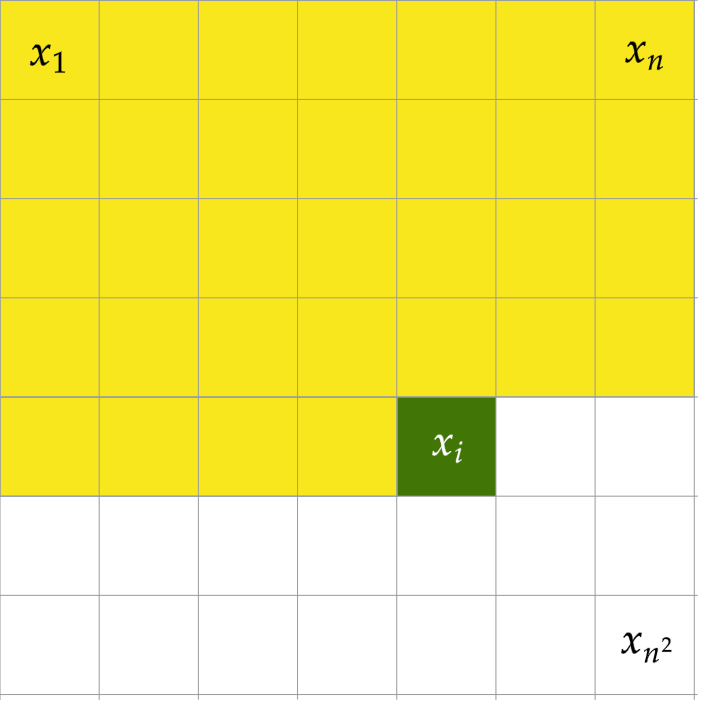
\includegraphics[scale=0.20]{figures/pixelcnn.png}
    \caption[Conditional generation in autoregressive models]%
    {Conditional generation in autoregressive models. The model generates the pixels of the image one at a time, conditioning on the previous pixels. The model is autoregressive, because the distribution of each pixel is conditioned on the previous pixels.}
  	\medskip 
    \hspace*{15pt}\hbox{\scriptsize Credit: Adapted from the original PixelCNN paper~\cite{pixelcnn}.}\label{PixelCNNFigure}
\end{figure}

The PixelCNN in the original architecture is a stack of fifteen fully convolutional network layers with masked convolutions. The masked convolutions are used to ensure that the model can only access the previous pixels, which is crucial for model to be autoregressive. The model is trained to minimize the negative log likelihood of the training data. The PixelCNNs have been shown to be very effective at capturing the distribution of the data. Most current state-of-the-art models use the PixelCNNs as a building block for example PixelCNN++ and PixelSNAIL~\cite{pixelcnn, pixelcnnpp,pixelsnail}.

\subsubsection{Application in VQ-VAEs}

The PixelCNNs are used in the VQ-VAEs to model the prior distribution $p_{\omega}(z)$ over the discrete latent variables. The prior distribution is trained to match the distribution of the latent variables $z$ sampled from the posterior distribution $q_{\phi}(z|x)$. The PixelCNN in combination with the VQ-VAEs has been shown to be exceptional at capturing the distribution of the latent variables and generating high resolution samples~\cite{vqvae}.


\subsection{Random number generation using Power law distribution}

Power law distribution in probability theory and statistics is a distribution in which one variable is proportional to a power of the other, i.e., 
$p(x) \propto x^{\alpha}$, where $x$ is the random variable and $\alpha$ is the exponent parameter, where $\alpha$ determines the shape of the distribution. The power law distribution is a heavy-tailed distribution, which means that the probability of the large values is higher than in the normal distribution. The power law distribution is used in various fields, such as physics, biology, economics, and computer science~\cite{powerlaw}. 

One example of the power law distribution could be the function $ f(x) = \alpha x^{\alpha - 1} $ for $ 0 \leq x \leq 1 $, $a > 0$. One advantage to this distribution is that this distribution has a finite range and is easy to scale to any range. This fact will be used when power law distribution is used to sample the number of pixels to be conditioned on in the semi-conditional VAEs.













\chapter{Methods}

This chapter will outline the methods of how SCVAEs and non-conditioned VAEs are
integrated using multitask learning in this thesis, which will be explored in
the context of images. The chapter will be divided into three sections. The first
section will describe the conditioning strategies, which will be used to
condition the VAEs. In the following section, I will describe the method of
merging SCVAEs with non-conditioned VAEs using two decoders, where one is
conditioned, and the other is not. This method will be referred to as
\method{1}. In the following section, I describe another method of merging
SCVAEs with non-conditioned VAEs by utilizing the same encoder and decoder for
both models by employing novel training strategies, which will be referred to
as \method{2}. Both methods will be applied to both Gaussian VAEs and VQ-VAEs.

\section{Conditioning information}

In this thesis, I will obtain the conditioning information $m$ from the input
image $x$ by sampling pixels some pixels from the input image $x$. In this
process, the first step is to obtain a mask which will be used to sample
the pixels from the input image $x$. The mask will be a binary matrix of the
same size as the input image $x$, where a value of 1 represents the sampled
pixels and a value of 0 represents the pixels that are not sampled. The
decision of how many pixels to sample and which pixels to sample will be described
in the following sections for each method.

After the mask is obtained, the mask is applied to the input image $x$ to
obtain the masked image, which is then used to obtain the conditioning
information $m$ by concatenating the mask with the masked image, which can be
seen in Figure~\ref{ConditioningFigure}.

In both proposed methods, the conditioning information $m$ will be incorporated
into the decoder by first flattening it and then concatenating it with the input of the decoder and then using a fully connected layer before passing it through the transposed convolutional layers of the decoder.

\begin{figure}
    \centering
    \tikzset{every picture/.style={line width=0.75pt}} %set default line width to 0.75pt        

\begin{tikzpicture}[x=0.75pt,y=0.75pt,yscale=-1,xscale=1]
%uncomment if require: \path (0,300); %set diagram left start at 0, and has height of 300

%Image [id:dp8071272108239995] 
\draw (189,81.67) node  {
\includegraphics[width=52.5pt,height=52.5pt]{figures/assets/ORIGINAL_GAUSSIAN.png}};
%Image [id:dp988855448482646] 
\draw (188.33,176) node  {
\includegraphics[width=52.5pt,height=52.5pt]{figures/assets/MASK_GAUSSIAN.png}};
%Image [id:dp22673392822113958] 
\draw (309.67,103.67) node  {
\includegraphics[width=52.5pt,height=52.5pt]{figures/assets/RESULT_GAUSSIAN.png}};
%Curve Lines [id:da7064061111049843] 
\draw    (224.33,86.33) .. controls (257.99,82.37) and (227.62,107.16) .. (272.29,100.54) ;
\draw [shift={(273.67,100.33)}, rotate = 171.07] [color={rgb, 255:red, 0; green, 0; blue, 0 }  ][line width=0.75]    (10.93,-3.29) .. controls (6.95,-1.4) and (3.31,-0.3) .. (0,0) .. controls (3.31,0.3) and (6.95,1.4) .. (10.93,3.29)   ;
%Curve Lines [id:da2412457613293979] 
\draw    (224.33,157.67) .. controls (273.83,153.05) and (228.59,124.9) .. (272.96,117.23) ;
\draw [shift={(274.33,117)}, rotate = 171.07] [color={rgb, 255:red, 0; green, 0; blue, 0 }  ][line width=0.75]    (10.93,-3.29) .. controls (6.95,-1.4) and (3.31,-0.3) .. (0,0) .. controls (3.31,0.3) and (6.95,1.4) .. (10.93,3.29)   ;
%Image [id:dp7901210362437346] 
\draw (431,111.33) node  {
\includegraphics[width=52.5pt,height=52.5pt]{figures/assets/GREEN_GAUSSIAN.png}};
%Image [id:dp9948313666469564] 
\draw (423.67,123) node  {
\includegraphics[width=52.5pt,height=52.5pt]{figures/assets/RED_GAUSSIAN.png}};
%Shape: Square [id:dp655934035728707] 
\draw  [color={rgb, 255:red, 255; green, 255; blue, 255 }  ,draw opacity=1 ] (388.67,88) -- (458.67,88) -- (458.67,158) -- (388.67,158) -- cycle ;
%Image [id:dp29091288526835224] 
\draw (417,136) node  {
\includegraphics[width=52.5pt,height=52.5pt]{figures/assets/BLUE_GAUSSIAN.png}};
%Shape: Square [id:dp17919766367981604] 
\draw  [color={rgb, 255:red, 255; green, 255; blue, 255 }  ,draw opacity=1 ] (382,101) -- (452,101) -- (452,171) -- (382,171) -- cycle ;
%Image [id:dp6261788477655241] 
\draw (411,148.67) node  {
\includegraphics[width=52.5pt,height=52.5pt]{figures/assets/MASK_GAUSSIAN.png}};
%Shape: Square [id:dp8527153376534193] 
\draw  [color={rgb, 255:red, 255; green, 255; blue, 255 }  ,draw opacity=1 ] (376,113.67) -- (446,113.67) -- (446,183.67) -- (376,183.67) -- cycle ;
%Curve Lines [id:da0011889641265926398] 
\draw    (345.67,104.33) .. controls (353.15,122.41) and (361.21,123.58) .. (369.86,125.84) ;
\draw [shift={(371.67,126.33)}, rotate = 195.95] [color={rgb, 255:red, 0; green, 0; blue, 0 }  ][line width=0.75]    (10.93,-3.29) .. controls (6.95,-1.4) and (3.31,-0.3) .. (0,0) .. controls (3.31,0.3) and (6.95,1.4) .. (10.93,3.29)   ;
%Curve Lines [id:da5210657288496086] 
\draw    (224.33,169.67) .. controls (267.89,153.83) and (323.87,157.59) .. (372.2,149.26) ;
\draw [shift={(373.67,149)}, rotate = 169.9] [color={rgb, 255:red, 0; green, 0; blue, 0 }  ][line width=0.75]    (10.93,-3.29) .. controls (6.95,-1.4) and (3.31,-0.3) .. (0,0) .. controls (3.31,0.3) and (6.95,1.4) .. (10.93,3.29)   ;

% Text Node
\draw (162,27.33) node [anchor=north west][inner sep=0.75pt]   [align=left] {Original};
% Text Node
\draw (168.67,123.33) node [anchor=north west][inner sep=0.75pt]   [align=left] {Mask};
% Text Node
\draw (420.67,50.67) node [anchor=north west][inner sep=0.75pt]   [align=left] {$\displaystyle m$};


\end{tikzpicture}

    \caption[The illustration of the process of obtaining the conditioning information $m$ from the input image $x$ and the mask.]%
    {
        The illustration of the process of obtaining the conditioning information $m$ from the input image $x$ and the mask. The process to obtain the conditioning information $m$ consists of two steps: the first step is to obtain the masked image from the input image $x$ and the mask, and the second step is to add the mask to the masked image to obtain the conditioning information $m$. The conditioning information $m$ is then used to condition the decoder.
    }\label{ConditioningFigure}
\end{figure}

\section{\method{1}}

In the first method, the VAE framework is expanded with a second decoder
$p_\xi(x|z,m)$, which is conditioned on an additional property $m$ of the input
data. This approach involves utilizing two decoders within the VAE framework:
one for reconstructing the input data solely based on a trained neural network with \method{1} latent variable $z$,
and the other for reconstructing the input data based on both the latent
variable $z$ and the additional conditioning information $m$.

\subsection{Conditioning strategy}

In this method, the conditioning information $m$ is acquired by sampling a
constant number of pixels from the input data. To sample the pixels from the
input image $x$, I will use a pixel sampling operation, which will be described
in the following section.

\subsubsection{Pixel Sampling operation}

I will explore two-pixel sampling types for this method,
which can be seen in Figure~\ref{SamplingFigure} and are described as follows:

\begin{enumerate}
    \item \textbf{Exact same sampling:} In this sampling type, the conditioning information $m$ is sampled from the input image $x$ by sampling the exact same sparse pixels from the input image $x$. In this work, the pixels that will be sampled from the input image will be a sparse grid of pixels.
    \item \textbf{Uniform random sampling:} In this sampling type, the conditioning information $m$ is sampled from the input image $x$ by sampling exact number of pixels from the input image $x$ uniformly at random.
\end{enumerate}

The sampling process will be done every time the input image $x$ is passed through the model. This means that in the case of the uniform random sampling, the conditioning information $m$ will be different for each time the image is passed through the model. This is done to ensure that the model learns to generalize and handle various cases.

\subsection{Application to Gaussian VAEs}

In Gaussian VAEs, the integration of a second conditioned decoder
$p_\xi(x|z,m)$ follows a similar approach as outlined in the general method
description. However, there are specific adjustments and considerations that
need to be taken into account when applying this method to Gaussian VAEs.

The integration of the second conditioned decoder $p_\xi(x|z,m)$ into the
Gaussian VAEs framework involves flattening on concatenating the latent
variable $z$ and the conditioning information $m$ and passing it through a
fully connected layer before passing it through the transposed convolutional
layers of the second decoder. Although a new latent variable could have
been sampled for the second decoder, the same latent variable $z$ is used
instead of sampling a new one. This is done to ensure that the latent variable
$z$ is the same for both decoders and ensures that it is easier to compare the
reconstructions of the input data. The architecture of the Gaussian
VAEs framework with the second conditioned decoder is illustrated in
Figure~\ref{SCVAE2DFigure}

Although the training strategy could have been to train decoders by alternating between them, in this thesis, I will explore the training strategy where both decoders are trained simultaneously.

In Gaussian VAEs, the loss objective consists of two components: the
reconstruction loss and the KL divergence term. However, with the inclusion of
the second conditioned decoder, the loss objective is extended to include the
reconstruction loss of the second conditioned decoder. The overall loss
objective to be \textbf{minimized} becomes

\[ L = W_1 \frac{1}{D} \sum_{i=1}^{D} ||x_i - \hat{x}_{1_{i}} ||^2 + W_2 \frac{1}{D} \sum_{i=1}^{D} || x_i - \hat{x}_{2_{i}} ||^2 + \beta  \frac{1}{2} \sum_{i=1}^{Z} \biggl( -\log \sigma^2_\phi(x)_i - 1 + \mu^2_\phi(x)_i + \sigma^2_\phi(x)_i \biggr), \]

where $D$ is the number of pixels in the input image, $x_i$ is the $i$-th pixel
of the input image, $\hat{x}_1$ is the output of the first decoder, $\hat{x}_2$
is the output of the second decoder, $\beta$ is the KL divergence weight, Z is
the dimension of the latent space, $\mu_\phi(x)$ and $\sigma_\phi(x)$ are the
mean and the standard deviation of the Gaussian distribution produced by the
encoder, respectively. The resulting loss has also extra weight parameters $W_1$ and $W_2$ to balance and control the importance of reconstruction loss, which will be hyperparameters of the model.

During the training process, the encoder is trained to produce an accurate mean
and standard deviation of the Gaussian distribution, and the decoders are
trained to produce accurate reconstructions of the input data. The KL
divergence term is used to regularize the latent space to be close to a
standard Gaussian distribution. The optimizer used to minimize the overall loss
objective is the AdamW optimizer~\cite{AdamW}.

As a result of the integration of the second conditioned decoder, the model has
the ability to reconstruct the input data based just on the latent variable $z$
and as well as the conditioning information $m$.
\begin{figure}[H]
    \centering
    \centering
\scriptsize
\begin{tabular}{||c|c|c|c||}
\hline
 Method & Parameters & Reconstruction loss & KL loss \\
\hline
\textit{Baseline} & - & 0.0042 +- 1.2e-03 & 0.0018 +- 6.3e-04 \\
\hline
Multi Decoder & Exact sampling & 0.0036 +- 8.3e-04  $\downarrow$ & 0.0027 +- 8.7e-04  $\uparrow$ \\
\hline
Multi Decoder & Exact sampling, SoftAdapt & 0.0034 +- 1.9e-04  $\downarrow$ & 0.0029 +- 2.8e-03  $\uparrow$ \\
\hline
Multi Decoder & Uniform sampling & 0.0035 +- 6.5e-04  $\downarrow$ & 0.0026 +- 1.7e-03  $\uparrow$ \\
\hline
Multi Decoder & Uniform sampling, SoftAdapt & 0.0034 +- 7.3e-03  $\downarrow$ & 0.0029 +- 2.0e-02  $\uparrow$ \\
\hline
\end{tabular}

    \caption[\method{1} applied to Gaussian VAEs.]%
    {
        \methodOne\ applied to Gaussian VAEs. The Gaussian VAEs framework is extended by adding a second conditioned decoder $p_\xi(x|z,m)$. The input $x$ is passed through the encoder with parameters $\phi$ producing the mean $\mu$ and the standard deviation $\sigma$ of the Gaussian distribution. The random variable $\epsilon$ is sampled from a standard Gaussian distribution and is used to sample $ z = \mu + \sigma \odot \epsilon$. The sampled $z$ is then used as input to both decoders. As a result, the loss function consists of three components: the MSE reconstruction loss of the first decoder, the MSE reconstruction loss of the second decoder and the KL divergence regularization loss.
    }\label{SCVAE2DFigure}
\end{figure}

\subsection{Application to VQ-VAEs}

The approach of integrating the second conditioned decoder $p_\xi(x|z,m)$ into
the VQ-VAEs framework is similar to the approach used for Gaussian VAEs.
However, some differences need to be taken into account when applying
this method to VQ-VAEs.

One of the main differences is that the VQ-VAEs framework uses a discrete
latent space and the Vector Quantization which is described in \autoref{background:vqvae}. This means that the latent variable $z$ is a discrete variable that represents the indexes of the embedding table vectors. This means that first the corresponding embedding table vectors $z_q(x)$ must be computed for the latent variable $z$ before flattening and concatenating it with the conditioning information $m$ and then using a fully connected layer before the transposed convolutional layers of the second decoder. The architecture of the VQ-VAEs framework with the second conditioned decoder is illustrated in Figure~\ref{SCVQVAE2DFigure}.

The training strategy is the same as in Gaussian VAEs, where both decoders are trained simultaneously. This means that the loss objective must be extended to include the reconstruction loss of the second conditioned decoder. In VQ-VAEs, the loss objective consists of three components: the MSE
reconstruction loss the commitment loss and the codebook loss. However,
with the inclusion of the second conditioned decoder, the loss objective is
extended to include the reconstruction loss of the second conditioned decoder.
The overall loss objective to be \textbf{minimized} becomes

\[ L = W_1 \frac{1}{D} \sum_{i=1}^{D} ||x_i - \hat{x}_{1_{i}} ||^2 +  W_2 \frac{1}{D} \sum_{i=1}^{D} || x_i - \hat{x}_{2_{i}} ||^2 + \frac{1}{Z} \sum_{i=1}^{Z} \biggl( || sg(z_e(x)_i) - e_{k_i} ||^2 + \beta || z_q(x)_i - sg(e_{k{_i}}) ||^2 \biggr) , \]

% TODO explain the weights W1 and W2

where $D$ is the number of pixels in the input image, $x_i$ is the $i$-th pixel
of the input image, $\hat{x}_1$ is the output of the first decoder, $\hat{x}_2$
is the output of the second decoder, $Z$ is the number of latent space vectors,
$z_e(x)$ is the output of the encoder, $z_q(x)$ is the mapping output after
Vector Quantization, $e_k$ is the $k$-th embedding table vector, $\beta$ is the
commitment loss weight, $sg$ is the stop gradient operation, which was
previously defined in the background \autoref{background:vqvae}.

After the first stage of the training, the model has the ability to reconstruct
the input data based just on the latent variable $z$ and as well as the
conditioning information $m$. To generate the latent variable $z$, one must be
trained a separate autoregressive model, which will be used to generate the
latent variable $z$.

\begin{figure}[H]
    \centering
    \centering
\scriptsize
\begin{tabular}{||c|c|c|c||}
\hline
 Method & Parameters & Reconstruction loss & VQ loss \\
\hline
\textit{Baseline} & - & 0.0022 +- 7.4e-08 & 0.0029 +- 4.1e-07 \\
\hline
Multi Decoder & Exact sampling & 0.0017 +- 6.9e-09  $\downarrow$ & 0.0039 +- 9.8e-07  $\uparrow$ \\
\hline
Multi Decoder & Exact sampling, SoftAdapt & \textbf{0.0013 +- 2.4e-09}  $\downarrow$ & \textbf{0.0016 +- 6.8e-08}  $\downarrow$ \\
\hline
Multi Decoder & Uniform sampling & 0.0018 +- 1.3e-07  $\downarrow$ & 0.0036 +- 3.5e-07  $\uparrow$ \\
\hline
Multi Decoder & Uniform sampling, SoftAdapt & \textbf{0.0017 +- 6.6e-08}  $\downarrow$ & \textbf{0.0021 +- 3.1e-07}  $\downarrow$ \\
\hline
\end{tabular}

    \caption[\method{1} applied to VQ-VAEs.]%
    {
        \method{1} applied to VQ-VAEs. The VQ-VAEs framework is extended by adding a second conditioned decoder. Instead of using a fully connected layer to merge the latent variable $z$ and the conditioning information $m$, the corresponding embedding table vectors $z_q(x)$ must be computed for the latent variable $z$ before merging it with the conditioning information $m$. As a result of adding the second conditioned decoder, the loss function requires the addition of the MSE reconstruction loss of the second decoder.
    }\label{SCVQVAE2DFigure}
\end{figure}

\section{\method{2}}

In the \method{2}, the idea is to employ a single decoder within the VAE architecture that is capable of reconstructing the input data under variable conditioning. Variable conditioning means that the conditioning information $m$ can be a variable amount of information or just an empty mask. This method differs from the \method{1} in that it uses a single decoder for both tasks and dynamically adjusts its behavior based on the amount of information present in the variable $m$.

This method utilizes a single decoder that dynamically adjusts its behavior
based on the amount of information present in the variable $m$. When the
conditioning information is available, the decoder incorporates it into the
reconstruction process and takes advantage of it to get the best
reconstruction. Otherwise, it operates solely based on the latent variable $z$.

To achieve this, in this method, I will use different conditioning strategies, which will be described in the following subsection.

\subsection{Conditioning strategy}

Similar to the previous method, the conditioning information $m$ is acquired by
sampling pixels from the input image $x$. However, in this method, the process of sampling the conditioning information $m$ is different in that the conditioning information $m$ is sampled by selecting a variable number of pixels from the input image $x$. This is done to ensure that the decoder of the model learns to handle various cases where there is variable conditioning information.

To achieve this, I will implement a two-step sampling process:

\begin{enumerate}
    \item \textbf{Sampling the number of pixels:} In this step, the number of pixels to be sampled from the input image $x$ is sampled from a power law distribution. The power law distribution is scaled to the size of the input image $x$ and is used to sample the number of pixels to be sampled from the input image $x$.
    \item \textbf{Sampling the pixels:} In this step, the conditioning information $m$ is sampled from the input image $x$ by sampling the number of pixels sampled in the previous step from the input image: uniformly at random or from a Gaussian distribution. Both of these sampling types can be seen in Figure~\ref{SamplingFigure}.
\end{enumerate}

The sampling two-step process will be done every time the input image $x$ is passed through the model. This means that the conditioning information $m$ will be different for each time the image is passed through the model. This is done to ensure that the model learns to generalize and handle various cases.

During training, the number of pixels to be sampled from the input image $x$ varies every time the input image $x$ is passed through the model and is sampled from a power law distribution.
The power law distribution is chosen because it can have a finite range and scalability, which makes it suitable for sampling the number of pixels from the input image. The exponent of the power law distribution will be chosen to be high so that the decoder can learn to handle also the cases where the conditioning information is not available. The exponent will be a hyperparameter of the model.


\subsection{Application to Gaussian VAEs}

In Gaussian VAEs, applying the second method involves modifying the decoder to
be capable of reconstructing the input data under variable conditioning. The
modified decoder $p_\xi(x|z,m)$ is capable of reconstructing the input data
based on the latent variable $z$ and the conditioning information $m$ or just
the latent variable $z$.

This is achieved by using a fully connected layer to merge the latent variable
$z$ and the conditioning information $m$ before passing it through the
transposed convolutional layers. The architecture of the Gaussian VAEs
framework with a single decoder capable of variable conditioning is illustrated
in Figure~\ref{SCVAE1DFigure}.

\begin{figure}[H]
    \centering
    \centering
\scriptsize
\begin{tabular}{||c|c|c|c||}
\hline
 Method & Parameters & Reconstruction loss & KL loss \\
\hline
\textit{Baseline} & - & 0.0097 +- 4.2e-03 & 63.0518 +- 2.4e+01 \\
\hline
Single Decoder & Gaussian sampling, Exponent=40 & 0.0113 +- 1.4e-02  $\uparrow$ & 54.7483 +- 7.3e+01  $\downarrow$ \\
\hline
Single Decoder & Gaussian sampling, Exponent=60 & 0.0113 +- 2.6e-03  $\uparrow$ & 54.6946 +- 4.4e+01  $\downarrow$ \\
\hline
\end{tabular}

    \caption[\method{2} applied to Gaussian VAEs.]%
    {
        \methodTwo\ applied to Gaussian VAEs. The Gaussian VAEs framework is modified by allowing the decoder to be conditioned on a variable amount of information and to dynamically adjust its behavior based on the amount of information present in the variable $m$. The input $x$ is passed through the encoder with parameters $\phi$ producing the mean $\mu$ and the standard deviation $\sigma$ of the Gaussian distribution. The random variable $\epsilon$ is sampled from a standard Gaussian distribution and is used to sample $ z = \mu + \sigma \odot \epsilon$. The sampled $z$ is then used as input to the decoder as well as the extra conditioning information $m$. With this approach, there is no need for a second decoder, as the single decoder is capable of reconstructing the data based on the latent variable $z$ and the conditioning information $m$ or just the latent variable $z$.
    }\label{SCVAE1DFigure}
\end{figure}

\subsection{Application to VQ-VAEs}

In VQVAEs, the same as in Gaussian VAEs, the second method involves modifying the
decoder to be capable of receiving variable conditioning information. Unlike
Gaussian VAEs, the VQ-VAEs use Vector Quantization to discretize the continuous 
latent space, which is described in \autoref{background:vqvae}. Since the latent
variable $z$ is just a representation of the indexes of the embedding table vectors, the latent variable $z$ must be first mapped to the corresponding embedding table vectors resulting in $z_q(x)$ representation. Then the same process as in Gaussian VAEs is applied where the latent variable $z_q(x)$ and the conditioning information $m$ are merged using a fully connected layer before passing it through the transposed convolutional layers of the decoder. The architecture of the VQ-VAEs framework with a single decoder capable of
variable conditioning is illustrated in Figure~\ref{SCVQVAE1DFigure}.

\begin{figure}[H]
    \centering
    \centering
\scriptsize
\begin{tabular}{||c|c|c|c||}
\hline
 Method & Parameters & Reconstruction loss & VQ loss \\
\hline
\textit{Baseline} & - & 0.0022 +- 4.2e-08 & 0.0048 +- 8.3e-07 \\
\hline
Single Decoder & Gaussian sampling, Exponent=40 & 0.0026 +- 1.9e-07  $\uparrow$ & 0.0028 +- 2.3e-06  $\downarrow$ \\
\hline
Single Decoder & Gaussian sampling, Exponent=40 & 0.0023 +- 3.9e-07  $\uparrow$ & 0.0015 +- 7.3e-08  $\downarrow$ \\
\hline
Single Decoder & Gaussian sampling, Exponent=60 & 0.0029 +- 4.5e-07  $\uparrow$ & 0.0041 +- 4.1e-06  $\downarrow$ \\
\hline
Single Decoder & Gaussian sampling, Exponent=60 & \textbf{0.0020 +- 9.2e-08}  $\downarrow$ & \textbf{0.0013 +- 7.6e-08}  $\downarrow$ \\
\hline
Single Decoder & Uniform sampling, Exponent=40 & \textbf{0.0022 +- 1.1e-08}  $\downarrow$ & \textbf{0.0020 +- 2.2e-08}  $\downarrow$ \\
\hline
Single Decoder & Uniform sampling, Exponent=40 & \textbf{0.0022 +- 1.2e-07}  $\downarrow$ & \textbf{0.0018 +- 1.1e-08}  $\downarrow$ \\
\hline
Single Decoder & Uniform sampling, Exponent=60 & 0.0026 +- 7.2e-08  $\uparrow$ & 0.0030 +- 8.0e-07  $\downarrow$ \\
\hline
Single Decoder & Uniform sampling, Exponent=60 & 0.0023 +- 2.1e-07  $\uparrow$ & 0.0015 +- 9.0e-08  $\downarrow$ \\
\hline
\end{tabular}

    \caption[\method{2} applied to VQ-VAEs.]%
    {
        \methodTwo\ applied to VQ-VAEs. The VQ-VAEs framework is modified by allowing the decoder to be conditioned on a variable amount of information and to dynamically adjust its behavior based on the amount of information present in the variable $m$. The input $x$ is passed through the encoder producing the output $z_e(x)$. The output $z_e(x)$ is then used as input to the autoregressive model to generate the latent variable $z$. The latent variable $z$ is then used as input to the decoder as well as the extra conditioning information $m$. With this approach, there is no need for a second decoder, as the single decoder is capable of reconstructing the data based on the latent variable $z$ and the conditioning information $m$ or just the latent variable $z$.
    }\label{SCVQVAE1DFigure}
\end{figure}

\begin{figure}
    \centering
    

\tikzset{every picture/.style={line width=0.75pt}} %set default line width to 0.75pt        

\begin{tikzpicture}[x=0.75pt,y=0.75pt,yscale=-1,xscale=1]
%uncomment if require: \path (0,374); %set diagram left start at 0, and has height of 374

%Image [id:dp9293884018723756] 
\draw (365.67,295.2) node  {
\includegraphics[width=225pt,height=75pt]{figures/assets/GAUSSIAN.png}};
%Image [id:dp548757972749888] 
\draw (365.67,208.8) node  {
\includegraphics[width=225pt,height=75pt]{figures/assets/UNIFORM.png}};
%Image [id:dp620494998311241] 
\draw (365.67,124.8) node  {
\includegraphics[width=225pt,height=75pt]{figures/assets/EXACT.png}};
%Shape: Grid [id:dp3074430629490833] 
\draw  [draw opacity=0] (242.67,82.33) -- (497.67,82.33) -- (497.67,337.67) -- (242.67,337.67) -- cycle ; \draw   (242.67,82.33) -- (242.67,337.67)(327.67,82.33) -- (327.67,337.67)(412.67,82.33) -- (412.67,337.67)(497.67,82.33) -- (497.67,337.67) ; \draw   (242.67,82.33) -- (497.67,82.33)(242.67,167.33) -- (497.67,167.33)(242.67,252.33) -- (497.67,252.33)(242.67,337.33) -- (497.67,337.33) ; \draw    ;

% Text Node
\draw (279.26,61.29) node [anchor=north west][inner sep=0.75pt]  [rotate=-308.3] [align=left] {original};
% Text Node
\draw (172.67,120) node [anchor=north west][inner sep=0.75pt]   [align=left] {Exact};
% Text Node
\draw (359.26,61.29) node [anchor=north west][inner sep=0.75pt]  [rotate=-308.3] [align=left] {original};
% Text Node
\draw (437.53,61.29) node [anchor=north west][inner sep=0.75pt]  [rotate=-308.3] [align=left] {original};
% Text Node
\draw (165.17,204) node [anchor=north west][inner sep=0.75pt]   [align=left] {Uniform};
% Text Node
\draw (160.17,291) node [anchor=north west][inner sep=0.75pt]   [align=left] {Gaussian};


\end{tikzpicture}

    \caption[Table of pixel sampling types for conditioning.]%
    {
        Table of pixel sampling types for conditioning. The table has 3 rows each representing a different sampling type. The first row represents the Exact Same Sampling type, the second row represents the uniform random sampling type and the third row represents the Gaussian sampling type where the pixels are more likely to be sampled from the center of the image. The first column represents the original image, the second column represents the mask and the third column represents the result of the sampling operation.
    }\label{SamplingFigure}
\end{figure}

\section{Experimental setup}

In this section, I will describe the experimental setup that will be used to evaluate the proposed methods.

\subsection{Datasets}

The proposed methods will be evaluated on the MNIST, CIFAR-10 and CelebA datasets. The MNIST dataset consists of 60,000 images of the size 28x28 pixels with 10 classes. The CIFAR-10 dataset consists of 60,000 colored images of the size 32x32 pixels with 10 classes.
The CelebA dataset consists of 202,599 images of celebrities with 10,177 identities and 40 binary attributes. In these experiments, the CelebA dataset images will be resized to 64x64 pixels to reduce the computational complexity.
The datasets will be split into training, validation and test sets, where the training set will be used to train the models and the validation set will be used to evaluate.

\subsection{Network architecture}

The encoder and the decoder of the models will be convolutional neural networks. The number of layers and the number of filters in each layer will be hyperparameters of the model. Both the encoder and the decoder will have a similar architecture of convolutional layers followed by batch normalization layers and LeakyReLU activation functions. However, the encoder and the decoder for the Gaussian VAEs will be more shallow compared to the VQ-VAEs, because the Gaussian VAEs suffer from the posterior collapse if the neural network is too deep. 

The latent space of the Gaussian VAEs will be 16 and 64 dimensions with 4 hidden layers with dimensions set to 32, 64, 128, and 256. 

The latent space of the VQ-VAEs will be with 16, 32 and 64 dimensions with 

\subsection{Training}

The models will be trained using the AdamW optimizer with a learning rate of $10^{-3}$ and a batch size of 128 for 100 epochs. The models will be trained on the training set and evaluated on the validation set. The best model will be selected based on the validation loss. The models will be trained on a single GPU.
\chapter{Results}

This chapter presents the findings of the experiments conducted in this master's thesis. The chapter is divided into two sections.
The first section presents the results of \methodOne{1}, and the second section presents the results of \methodTwo{2}, where both methods will be evaluated in the context of both Gaussian VAEs and VQ-VAEs. In the final section, I will present the cross-validation results of both methods on all datasets and configurations in this thesis.

\section{Results of \methodOne{1}}

In this section, I will present the results of applying \methodOne{1} on both Gaussian VAEs and VQ-VAEs, with a comparative analysis of the baseline models without the method applied. The primary performance metrics that we will focus on are the reconstruction loss and the KL divergence loss of the latent space in the case of Gaussian VAEs and the VQ objective loss in the case of VQ-VAEs. 

The results presented in this section are based on the experiments conducted on the CelebA dataset with Config. 2 for Gaussian VAEs and Config. 3 for VQ-VAEs. The results on other configurations showed similar results with minor differences and can be found in the last section of this chapter~\ref{sec:cross_val_results}. The experiments will be compared and analyzed with respect to both Exact Sampling and Uniform Sampling and tested with the SoftAdapt loss balancing technique and without it. 

\subsection{Results on Gaussian VAEs}

The experiments unveiled the effectiveness of \methodOne{1} on Gaussian VAEs in fulfilling its core task of training two decoders with a shared encoder. Upon analysis, it became evident that the implementation of \methodOne{1} successfully reduced the reconstruction loss for both the conditioned and non-conditioned decoders. However, it was observed that the KL divergence loss of the latent space increased with the application of \methodOne{1}, which can be seen in figure \ref{fig:results_method1_gaussian_vae} and table \ref{tab:results_method1_gaussian_vae}.

Remarkably, as expected, the conditioned decoder consistently produced higher-quality reconstructions compared to its non-conditioned counterpart, as evidenced by the figure~\ref{fig:rec_gaussian}. Further comparison between the Exact Sampling and Uniform Sampling methods revealed minimal differences in the results, as shown in table \ref{tab:results_method1_gaussian_vae}.

Moreover, the experiments explored the impact of employing the SoftAdapt loss balancing technique. Surprisingly, in this case, the results showed negligible differences between its application and the absence of it. However, the utilization of SoftAdapt appeared to stabilize the training process by reducing fluctuations in the losses.

Additionally, experiments involving deeper neural networks unveiled a higher likelihood of training instability in the form of posterior collapse - a common challenge encountered in Gaussian VAEs~\cite{wang2023posterior}. Consequently, a more sophisticated configuration of a Gaussian VAE was deemed unsuitable for the experiments.

\begin{table}[H]
    \centering
    \centering
\scriptsize
\begin{tabular}{||c|c|c|c||}
\hline
 Method & Parameters & Reconstruction loss & KL loss \\
\hline
\textit{Baseline} & - & 0.0042 +- 1.2e-03 & 0.0018 +- 6.3e-04 \\
\hline
Multi Decoder & Exact sampling & 0.0036 +- 8.3e-04  $\downarrow$ & 0.0027 +- 8.7e-04  $\uparrow$ \\
\hline
Multi Decoder & Exact sampling, SoftAdapt & 0.0034 +- 1.9e-04  $\downarrow$ & 0.0029 +- 2.8e-03  $\uparrow$ \\
\hline
Multi Decoder & Uniform sampling & 0.0035 +- 6.5e-04  $\downarrow$ & 0.0026 +- 1.7e-03  $\uparrow$ \\
\hline
Multi Decoder & Uniform sampling, SoftAdapt & 0.0034 +- 7.3e-03  $\downarrow$ & 0.0029 +- 2.0e-02  $\uparrow$ \\
\hline
\end{tabular}

    \caption{Cross-validation results of \methodOne{1} applied to a Gaussian VAE(Config. 2) on the CelebA dataset.}
    \label{tab:results_method1_gaussian_vae}
\end{table}

\begin{figure}[H]
    \centering
    \scalebox{0.48}{%% Creator: Matplotlib, PGF backend
%%
%% To include the figure in your LaTeX document, write
%%   \input{<filename>.pgf}
%%
%% Make sure the required packages are loaded in your preamble
%%   \usepackage{pgf}
%%
%% Also ensure that all the required font packages are loaded; for instance,
%% the lmodern package is sometimes necessary when using math font.
%%   \usepackage{lmodern}
%%
%% Figures using additional raster images can only be included by \input if
%% they are in the same directory as the main LaTeX file. For loading figures
%% from other directories you can use the `import` package
%%   \usepackage{import}
%%
%% and then include the figures with
%%   \import{<path to file>}{<filename>.pgf}
%%
%% Matplotlib used the following preamble
%%   
%%   \usepackage{fontspec}
%%   \setmainfont{DejaVuSerif.ttf}[Path=\detokenize{/home/edvardsz/miniconda3/envs/pytorch-latest/lib/python3.10/site-packages/matplotlib/mpl-data/fonts/ttf/}]
%%   \setsansfont{DejaVuSans.ttf}[Path=\detokenize{/home/edvardsz/miniconda3/envs/pytorch-latest/lib/python3.10/site-packages/matplotlib/mpl-data/fonts/ttf/}]
%%   \setmonofont{DejaVuSansMono.ttf}[Path=\detokenize{/home/edvardsz/miniconda3/envs/pytorch-latest/lib/python3.10/site-packages/matplotlib/mpl-data/fonts/ttf/}]
%%   \makeatletter\@ifpackageloaded{underscore}{}{\usepackage[strings]{underscore}}\makeatother
%%
\begingroup%
\makeatletter%
\begin{pgfpicture}%
\pgfpathrectangle{\pgfpointorigin}{\pgfqpoint{6.400000in}{4.800000in}}%
\pgfusepath{use as bounding box, clip}%
\begin{pgfscope}%
\pgfsetbuttcap%
\pgfsetmiterjoin%
\definecolor{currentfill}{rgb}{1.000000,1.000000,1.000000}%
\pgfsetfillcolor{currentfill}%
\pgfsetlinewidth{0.000000pt}%
\definecolor{currentstroke}{rgb}{1.000000,1.000000,1.000000}%
\pgfsetstrokecolor{currentstroke}%
\pgfsetdash{}{0pt}%
\pgfpathmoveto{\pgfqpoint{0.000000in}{0.000000in}}%
\pgfpathlineto{\pgfqpoint{6.400000in}{0.000000in}}%
\pgfpathlineto{\pgfqpoint{6.400000in}{4.800000in}}%
\pgfpathlineto{\pgfqpoint{0.000000in}{4.800000in}}%
\pgfpathlineto{\pgfqpoint{0.000000in}{0.000000in}}%
\pgfpathclose%
\pgfusepath{fill}%
\end{pgfscope}%
\begin{pgfscope}%
\pgfsetbuttcap%
\pgfsetmiterjoin%
\definecolor{currentfill}{rgb}{1.000000,1.000000,1.000000}%
\pgfsetfillcolor{currentfill}%
\pgfsetlinewidth{0.000000pt}%
\definecolor{currentstroke}{rgb}{0.000000,0.000000,0.000000}%
\pgfsetstrokecolor{currentstroke}%
\pgfsetstrokeopacity{0.000000}%
\pgfsetdash{}{0pt}%
\pgfpathmoveto{\pgfqpoint{0.800000in}{0.528000in}}%
\pgfpathlineto{\pgfqpoint{5.760000in}{0.528000in}}%
\pgfpathlineto{\pgfqpoint{5.760000in}{4.224000in}}%
\pgfpathlineto{\pgfqpoint{0.800000in}{4.224000in}}%
\pgfpathlineto{\pgfqpoint{0.800000in}{0.528000in}}%
\pgfpathclose%
\pgfusepath{fill}%
\end{pgfscope}%
\begin{pgfscope}%
\pgfpathrectangle{\pgfqpoint{0.800000in}{0.528000in}}{\pgfqpoint{4.960000in}{3.696000in}}%
\pgfusepath{clip}%
\pgfsetbuttcap%
\pgfsetroundjoin%
\definecolor{currentfill}{rgb}{0.121569,0.466667,0.705882}%
\pgfsetfillcolor{currentfill}%
\pgfsetfillopacity{0.200000}%
\pgfsetlinewidth{0.000000pt}%
\definecolor{currentstroke}{rgb}{0.000000,0.000000,0.000000}%
\pgfsetstrokecolor{currentstroke}%
\pgfsetdash{}{0pt}%
\pgfpathmoveto{\pgfqpoint{1.025455in}{3.929189in}}%
\pgfpathlineto{\pgfqpoint{1.025455in}{3.537991in}}%
\pgfpathlineto{\pgfqpoint{1.071001in}{3.122283in}}%
\pgfpathlineto{\pgfqpoint{1.116547in}{2.832449in}}%
\pgfpathlineto{\pgfqpoint{1.162094in}{2.903462in}}%
\pgfpathlineto{\pgfqpoint{1.207640in}{2.687249in}}%
\pgfpathlineto{\pgfqpoint{1.253186in}{2.916588in}}%
\pgfpathlineto{\pgfqpoint{1.298733in}{3.033231in}}%
\pgfpathlineto{\pgfqpoint{1.344279in}{3.015861in}}%
\pgfpathlineto{\pgfqpoint{1.389826in}{2.836476in}}%
\pgfpathlineto{\pgfqpoint{1.435372in}{3.085044in}}%
\pgfpathlineto{\pgfqpoint{1.480918in}{2.915581in}}%
\pgfpathlineto{\pgfqpoint{1.526465in}{3.127264in}}%
\pgfpathlineto{\pgfqpoint{1.572011in}{3.169460in}}%
\pgfpathlineto{\pgfqpoint{1.617557in}{3.207472in}}%
\pgfpathlineto{\pgfqpoint{1.663104in}{3.187534in}}%
\pgfpathlineto{\pgfqpoint{1.708650in}{3.240190in}}%
\pgfpathlineto{\pgfqpoint{1.754197in}{3.134822in}}%
\pgfpathlineto{\pgfqpoint{1.799743in}{3.259595in}}%
\pgfpathlineto{\pgfqpoint{1.845289in}{3.194550in}}%
\pgfpathlineto{\pgfqpoint{1.890836in}{3.211237in}}%
\pgfpathlineto{\pgfqpoint{1.936382in}{3.121448in}}%
\pgfpathlineto{\pgfqpoint{1.981928in}{3.302009in}}%
\pgfpathlineto{\pgfqpoint{2.027475in}{3.157058in}}%
\pgfpathlineto{\pgfqpoint{2.073021in}{3.193563in}}%
\pgfpathlineto{\pgfqpoint{2.118567in}{3.204020in}}%
\pgfpathlineto{\pgfqpoint{2.164114in}{3.235871in}}%
\pgfpathlineto{\pgfqpoint{2.209660in}{3.219401in}}%
\pgfpathlineto{\pgfqpoint{2.255207in}{3.155879in}}%
\pgfpathlineto{\pgfqpoint{2.300753in}{3.140057in}}%
\pgfpathlineto{\pgfqpoint{2.346299in}{3.276677in}}%
\pgfpathlineto{\pgfqpoint{2.391846in}{3.248486in}}%
\pgfpathlineto{\pgfqpoint{2.437392in}{3.232774in}}%
\pgfpathlineto{\pgfqpoint{2.482938in}{3.120404in}}%
\pgfpathlineto{\pgfqpoint{2.528485in}{3.108912in}}%
\pgfpathlineto{\pgfqpoint{2.574031in}{3.259645in}}%
\pgfpathlineto{\pgfqpoint{2.619578in}{3.191275in}}%
\pgfpathlineto{\pgfqpoint{2.665124in}{3.147473in}}%
\pgfpathlineto{\pgfqpoint{2.710670in}{3.066586in}}%
\pgfpathlineto{\pgfqpoint{2.756217in}{3.010422in}}%
\pgfpathlineto{\pgfqpoint{2.801763in}{3.149030in}}%
\pgfpathlineto{\pgfqpoint{2.847309in}{3.045395in}}%
\pgfpathlineto{\pgfqpoint{2.892856in}{3.130408in}}%
\pgfpathlineto{\pgfqpoint{2.938402in}{3.117338in}}%
\pgfpathlineto{\pgfqpoint{2.983949in}{3.053296in}}%
\pgfpathlineto{\pgfqpoint{3.029495in}{3.087232in}}%
\pgfpathlineto{\pgfqpoint{3.075041in}{3.135152in}}%
\pgfpathlineto{\pgfqpoint{3.120588in}{3.023087in}}%
\pgfpathlineto{\pgfqpoint{3.166134in}{3.077993in}}%
\pgfpathlineto{\pgfqpoint{3.211680in}{3.024365in}}%
\pgfpathlineto{\pgfqpoint{3.257227in}{3.012424in}}%
\pgfpathlineto{\pgfqpoint{3.302773in}{3.102255in}}%
\pgfpathlineto{\pgfqpoint{3.348320in}{2.918863in}}%
\pgfpathlineto{\pgfqpoint{3.393866in}{3.008511in}}%
\pgfpathlineto{\pgfqpoint{3.439412in}{2.955032in}}%
\pgfpathlineto{\pgfqpoint{3.484959in}{3.092520in}}%
\pgfpathlineto{\pgfqpoint{3.530505in}{3.154943in}}%
\pgfpathlineto{\pgfqpoint{3.576051in}{2.996920in}}%
\pgfpathlineto{\pgfqpoint{3.621598in}{2.965495in}}%
\pgfpathlineto{\pgfqpoint{3.667144in}{2.994105in}}%
\pgfpathlineto{\pgfqpoint{3.712691in}{3.117368in}}%
\pgfpathlineto{\pgfqpoint{3.758237in}{2.884299in}}%
\pgfpathlineto{\pgfqpoint{3.803783in}{3.117592in}}%
\pgfpathlineto{\pgfqpoint{3.849330in}{3.041827in}}%
\pgfpathlineto{\pgfqpoint{3.894876in}{3.030016in}}%
\pgfpathlineto{\pgfqpoint{3.940422in}{3.005681in}}%
\pgfpathlineto{\pgfqpoint{3.985969in}{3.048484in}}%
\pgfpathlineto{\pgfqpoint{4.031515in}{2.957451in}}%
\pgfpathlineto{\pgfqpoint{4.077062in}{3.068909in}}%
\pgfpathlineto{\pgfqpoint{4.122608in}{3.057460in}}%
\pgfpathlineto{\pgfqpoint{4.168154in}{3.083402in}}%
\pgfpathlineto{\pgfqpoint{4.213701in}{3.053520in}}%
\pgfpathlineto{\pgfqpoint{4.259247in}{2.932866in}}%
\pgfpathlineto{\pgfqpoint{4.304793in}{3.006902in}}%
\pgfpathlineto{\pgfqpoint{4.350340in}{2.963090in}}%
\pgfpathlineto{\pgfqpoint{4.395886in}{3.018513in}}%
\pgfpathlineto{\pgfqpoint{4.441433in}{2.923496in}}%
\pgfpathlineto{\pgfqpoint{4.486979in}{3.091054in}}%
\pgfpathlineto{\pgfqpoint{4.532525in}{2.998805in}}%
\pgfpathlineto{\pgfqpoint{4.578072in}{3.017427in}}%
\pgfpathlineto{\pgfqpoint{4.623618in}{3.009680in}}%
\pgfpathlineto{\pgfqpoint{4.669164in}{2.940754in}}%
\pgfpathlineto{\pgfqpoint{4.714711in}{3.003876in}}%
\pgfpathlineto{\pgfqpoint{4.760257in}{3.080449in}}%
\pgfpathlineto{\pgfqpoint{4.805803in}{2.881042in}}%
\pgfpathlineto{\pgfqpoint{4.851350in}{3.089797in}}%
\pgfpathlineto{\pgfqpoint{4.896896in}{3.097966in}}%
\pgfpathlineto{\pgfqpoint{4.942443in}{3.080417in}}%
\pgfpathlineto{\pgfqpoint{4.987989in}{3.028506in}}%
\pgfpathlineto{\pgfqpoint{5.033535in}{3.030086in}}%
\pgfpathlineto{\pgfqpoint{5.079082in}{3.126308in}}%
\pgfpathlineto{\pgfqpoint{5.124628in}{3.093430in}}%
\pgfpathlineto{\pgfqpoint{5.170174in}{3.023292in}}%
\pgfpathlineto{\pgfqpoint{5.215721in}{2.843369in}}%
\pgfpathlineto{\pgfqpoint{5.261267in}{3.111639in}}%
\pgfpathlineto{\pgfqpoint{5.306814in}{3.074169in}}%
\pgfpathlineto{\pgfqpoint{5.352360in}{2.982174in}}%
\pgfpathlineto{\pgfqpoint{5.397906in}{2.900721in}}%
\pgfpathlineto{\pgfqpoint{5.443453in}{2.937953in}}%
\pgfpathlineto{\pgfqpoint{5.488999in}{2.999501in}}%
\pgfpathlineto{\pgfqpoint{5.534545in}{2.906677in}}%
\pgfpathlineto{\pgfqpoint{5.534545in}{3.420978in}}%
\pgfpathlineto{\pgfqpoint{5.534545in}{3.420978in}}%
\pgfpathlineto{\pgfqpoint{5.488999in}{3.358298in}}%
\pgfpathlineto{\pgfqpoint{5.443453in}{3.258480in}}%
\pgfpathlineto{\pgfqpoint{5.397906in}{3.387737in}}%
\pgfpathlineto{\pgfqpoint{5.352360in}{3.578332in}}%
\pgfpathlineto{\pgfqpoint{5.306814in}{3.273723in}}%
\pgfpathlineto{\pgfqpoint{5.261267in}{3.255319in}}%
\pgfpathlineto{\pgfqpoint{5.215721in}{3.335540in}}%
\pgfpathlineto{\pgfqpoint{5.170174in}{3.262451in}}%
\pgfpathlineto{\pgfqpoint{5.124628in}{3.250591in}}%
\pgfpathlineto{\pgfqpoint{5.079082in}{3.508184in}}%
\pgfpathlineto{\pgfqpoint{5.033535in}{3.315780in}}%
\pgfpathlineto{\pgfqpoint{4.987989in}{3.443437in}}%
\pgfpathlineto{\pgfqpoint{4.942443in}{3.351581in}}%
\pgfpathlineto{\pgfqpoint{4.896896in}{3.293024in}}%
\pgfpathlineto{\pgfqpoint{4.851350in}{3.280838in}}%
\pgfpathlineto{\pgfqpoint{4.805803in}{3.360815in}}%
\pgfpathlineto{\pgfqpoint{4.760257in}{3.506281in}}%
\pgfpathlineto{\pgfqpoint{4.714711in}{3.301647in}}%
\pgfpathlineto{\pgfqpoint{4.669164in}{3.275831in}}%
\pgfpathlineto{\pgfqpoint{4.623618in}{3.314779in}}%
\pgfpathlineto{\pgfqpoint{4.578072in}{3.440974in}}%
\pgfpathlineto{\pgfqpoint{4.532525in}{3.304433in}}%
\pgfpathlineto{\pgfqpoint{4.486979in}{3.390078in}}%
\pgfpathlineto{\pgfqpoint{4.441433in}{3.289462in}}%
\pgfpathlineto{\pgfqpoint{4.395886in}{3.543476in}}%
\pgfpathlineto{\pgfqpoint{4.350340in}{3.448679in}}%
\pgfpathlineto{\pgfqpoint{4.304793in}{3.320934in}}%
\pgfpathlineto{\pgfqpoint{4.259247in}{3.394467in}}%
\pgfpathlineto{\pgfqpoint{4.213701in}{3.312161in}}%
\pgfpathlineto{\pgfqpoint{4.168154in}{3.371584in}}%
\pgfpathlineto{\pgfqpoint{4.122608in}{3.300060in}}%
\pgfpathlineto{\pgfqpoint{4.077062in}{3.219078in}}%
\pgfpathlineto{\pgfqpoint{4.031515in}{3.363309in}}%
\pgfpathlineto{\pgfqpoint{3.985969in}{3.361689in}}%
\pgfpathlineto{\pgfqpoint{3.940422in}{3.277855in}}%
\pgfpathlineto{\pgfqpoint{3.894876in}{3.427965in}}%
\pgfpathlineto{\pgfqpoint{3.849330in}{3.444936in}}%
\pgfpathlineto{\pgfqpoint{3.803783in}{3.272595in}}%
\pgfpathlineto{\pgfqpoint{3.758237in}{3.330419in}}%
\pgfpathlineto{\pgfqpoint{3.712691in}{3.450005in}}%
\pgfpathlineto{\pgfqpoint{3.667144in}{3.317216in}}%
\pgfpathlineto{\pgfqpoint{3.621598in}{3.315553in}}%
\pgfpathlineto{\pgfqpoint{3.576051in}{3.502008in}}%
\pgfpathlineto{\pgfqpoint{3.530505in}{3.363480in}}%
\pgfpathlineto{\pgfqpoint{3.484959in}{3.876449in}}%
\pgfpathlineto{\pgfqpoint{3.439412in}{3.566686in}}%
\pgfpathlineto{\pgfqpoint{3.393866in}{3.315729in}}%
\pgfpathlineto{\pgfqpoint{3.348320in}{3.253276in}}%
\pgfpathlineto{\pgfqpoint{3.302773in}{3.317416in}}%
\pgfpathlineto{\pgfqpoint{3.257227in}{3.191466in}}%
\pgfpathlineto{\pgfqpoint{3.211680in}{3.250683in}}%
\pgfpathlineto{\pgfqpoint{3.166134in}{3.263858in}}%
\pgfpathlineto{\pgfqpoint{3.120588in}{3.316533in}}%
\pgfpathlineto{\pgfqpoint{3.075041in}{3.397955in}}%
\pgfpathlineto{\pgfqpoint{3.029495in}{3.303393in}}%
\pgfpathlineto{\pgfqpoint{2.983949in}{3.324609in}}%
\pgfpathlineto{\pgfqpoint{2.938402in}{3.540281in}}%
\pgfpathlineto{\pgfqpoint{2.892856in}{3.968047in}}%
\pgfpathlineto{\pgfqpoint{2.847309in}{3.839867in}}%
\pgfpathlineto{\pgfqpoint{2.801763in}{3.689975in}}%
\pgfpathlineto{\pgfqpoint{2.756217in}{3.428790in}}%
\pgfpathlineto{\pgfqpoint{2.710670in}{3.435124in}}%
\pgfpathlineto{\pgfqpoint{2.665124in}{3.465472in}}%
\pgfpathlineto{\pgfqpoint{2.619578in}{3.407025in}}%
\pgfpathlineto{\pgfqpoint{2.574031in}{3.435495in}}%
\pgfpathlineto{\pgfqpoint{2.528485in}{3.449898in}}%
\pgfpathlineto{\pgfqpoint{2.482938in}{3.363948in}}%
\pgfpathlineto{\pgfqpoint{2.437392in}{3.395517in}}%
\pgfpathlineto{\pgfqpoint{2.391846in}{3.422574in}}%
\pgfpathlineto{\pgfqpoint{2.346299in}{3.550113in}}%
\pgfpathlineto{\pgfqpoint{2.300753in}{3.367676in}}%
\pgfpathlineto{\pgfqpoint{2.255207in}{3.403017in}}%
\pgfpathlineto{\pgfqpoint{2.209660in}{3.445062in}}%
\pgfpathlineto{\pgfqpoint{2.164114in}{3.374658in}}%
\pgfpathlineto{\pgfqpoint{2.118567in}{3.351696in}}%
\pgfpathlineto{\pgfqpoint{2.073021in}{3.384680in}}%
\pgfpathlineto{\pgfqpoint{2.027475in}{3.346582in}}%
\pgfpathlineto{\pgfqpoint{1.981928in}{3.436433in}}%
\pgfpathlineto{\pgfqpoint{1.936382in}{3.357414in}}%
\pgfpathlineto{\pgfqpoint{1.890836in}{3.442864in}}%
\pgfpathlineto{\pgfqpoint{1.845289in}{3.381247in}}%
\pgfpathlineto{\pgfqpoint{1.799743in}{3.447560in}}%
\pgfpathlineto{\pgfqpoint{1.754197in}{3.427583in}}%
\pgfpathlineto{\pgfqpoint{1.708650in}{3.370926in}}%
\pgfpathlineto{\pgfqpoint{1.663104in}{3.484389in}}%
\pgfpathlineto{\pgfqpoint{1.617557in}{3.488997in}}%
\pgfpathlineto{\pgfqpoint{1.572011in}{3.345366in}}%
\pgfpathlineto{\pgfqpoint{1.526465in}{3.212384in}}%
\pgfpathlineto{\pgfqpoint{1.480918in}{3.412493in}}%
\pgfpathlineto{\pgfqpoint{1.435372in}{3.205538in}}%
\pgfpathlineto{\pgfqpoint{1.389826in}{3.398463in}}%
\pgfpathlineto{\pgfqpoint{1.344279in}{3.292534in}}%
\pgfpathlineto{\pgfqpoint{1.298733in}{3.685381in}}%
\pgfpathlineto{\pgfqpoint{1.253186in}{3.833992in}}%
\pgfpathlineto{\pgfqpoint{1.207640in}{3.902895in}}%
\pgfpathlineto{\pgfqpoint{1.162094in}{4.056000in}}%
\pgfpathlineto{\pgfqpoint{1.116547in}{3.900036in}}%
\pgfpathlineto{\pgfqpoint{1.071001in}{3.584985in}}%
\pgfpathlineto{\pgfqpoint{1.025455in}{3.929189in}}%
\pgfpathlineto{\pgfqpoint{1.025455in}{3.929189in}}%
\pgfpathclose%
\pgfusepath{fill}%
\end{pgfscope}%
\begin{pgfscope}%
\pgfpathrectangle{\pgfqpoint{0.800000in}{0.528000in}}{\pgfqpoint{4.960000in}{3.696000in}}%
\pgfusepath{clip}%
\pgfsetbuttcap%
\pgfsetroundjoin%
\definecolor{currentfill}{rgb}{1.000000,0.498039,0.054902}%
\pgfsetfillcolor{currentfill}%
\pgfsetfillopacity{0.200000}%
\pgfsetlinewidth{0.000000pt}%
\definecolor{currentstroke}{rgb}{0.000000,0.000000,0.000000}%
\pgfsetstrokecolor{currentstroke}%
\pgfsetdash{}{0pt}%
\pgfpathmoveto{\pgfqpoint{1.025455in}{1.683168in}}%
\pgfpathlineto{\pgfqpoint{1.025455in}{1.047629in}}%
\pgfpathlineto{\pgfqpoint{1.071001in}{0.969303in}}%
\pgfpathlineto{\pgfqpoint{1.116547in}{1.016813in}}%
\pgfpathlineto{\pgfqpoint{1.162094in}{0.781468in}}%
\pgfpathlineto{\pgfqpoint{1.207640in}{0.839402in}}%
\pgfpathlineto{\pgfqpoint{1.253186in}{0.846950in}}%
\pgfpathlineto{\pgfqpoint{1.298733in}{0.818006in}}%
\pgfpathlineto{\pgfqpoint{1.344279in}{0.727470in}}%
\pgfpathlineto{\pgfqpoint{1.389826in}{0.845338in}}%
\pgfpathlineto{\pgfqpoint{1.435372in}{0.922237in}}%
\pgfpathlineto{\pgfqpoint{1.480918in}{0.769583in}}%
\pgfpathlineto{\pgfqpoint{1.526465in}{0.866811in}}%
\pgfpathlineto{\pgfqpoint{1.572011in}{0.918293in}}%
\pgfpathlineto{\pgfqpoint{1.617557in}{1.005203in}}%
\pgfpathlineto{\pgfqpoint{1.663104in}{0.947155in}}%
\pgfpathlineto{\pgfqpoint{1.708650in}{1.010019in}}%
\pgfpathlineto{\pgfqpoint{1.754197in}{0.941294in}}%
\pgfpathlineto{\pgfqpoint{1.799743in}{0.925278in}}%
\pgfpathlineto{\pgfqpoint{1.845289in}{1.007115in}}%
\pgfpathlineto{\pgfqpoint{1.890836in}{0.966558in}}%
\pgfpathlineto{\pgfqpoint{1.936382in}{0.918837in}}%
\pgfpathlineto{\pgfqpoint{1.981928in}{0.892125in}}%
\pgfpathlineto{\pgfqpoint{2.027475in}{0.921142in}}%
\pgfpathlineto{\pgfqpoint{2.073021in}{0.938074in}}%
\pgfpathlineto{\pgfqpoint{2.118567in}{0.835178in}}%
\pgfpathlineto{\pgfqpoint{2.164114in}{0.970814in}}%
\pgfpathlineto{\pgfqpoint{2.209660in}{0.901353in}}%
\pgfpathlineto{\pgfqpoint{2.255207in}{0.877781in}}%
\pgfpathlineto{\pgfqpoint{2.300753in}{0.946693in}}%
\pgfpathlineto{\pgfqpoint{2.346299in}{1.021244in}}%
\pgfpathlineto{\pgfqpoint{2.391846in}{1.002423in}}%
\pgfpathlineto{\pgfqpoint{2.437392in}{0.964962in}}%
\pgfpathlineto{\pgfqpoint{2.482938in}{1.020770in}}%
\pgfpathlineto{\pgfqpoint{2.528485in}{0.832518in}}%
\pgfpathlineto{\pgfqpoint{2.574031in}{0.999805in}}%
\pgfpathlineto{\pgfqpoint{2.619578in}{0.919729in}}%
\pgfpathlineto{\pgfqpoint{2.665124in}{0.943501in}}%
\pgfpathlineto{\pgfqpoint{2.710670in}{0.923277in}}%
\pgfpathlineto{\pgfqpoint{2.756217in}{0.820573in}}%
\pgfpathlineto{\pgfqpoint{2.801763in}{0.973788in}}%
\pgfpathlineto{\pgfqpoint{2.847309in}{0.949228in}}%
\pgfpathlineto{\pgfqpoint{2.892856in}{0.923273in}}%
\pgfpathlineto{\pgfqpoint{2.938402in}{0.887630in}}%
\pgfpathlineto{\pgfqpoint{2.983949in}{0.930689in}}%
\pgfpathlineto{\pgfqpoint{3.029495in}{0.821771in}}%
\pgfpathlineto{\pgfqpoint{3.075041in}{0.864723in}}%
\pgfpathlineto{\pgfqpoint{3.120588in}{0.933676in}}%
\pgfpathlineto{\pgfqpoint{3.166134in}{0.874988in}}%
\pgfpathlineto{\pgfqpoint{3.211680in}{0.909982in}}%
\pgfpathlineto{\pgfqpoint{3.257227in}{0.909882in}}%
\pgfpathlineto{\pgfqpoint{3.302773in}{0.901347in}}%
\pgfpathlineto{\pgfqpoint{3.348320in}{0.894787in}}%
\pgfpathlineto{\pgfqpoint{3.393866in}{0.840882in}}%
\pgfpathlineto{\pgfqpoint{3.439412in}{0.863520in}}%
\pgfpathlineto{\pgfqpoint{3.484959in}{0.836132in}}%
\pgfpathlineto{\pgfqpoint{3.530505in}{0.849308in}}%
\pgfpathlineto{\pgfqpoint{3.576051in}{0.833351in}}%
\pgfpathlineto{\pgfqpoint{3.621598in}{0.833120in}}%
\pgfpathlineto{\pgfqpoint{3.667144in}{0.909248in}}%
\pgfpathlineto{\pgfqpoint{3.712691in}{0.854889in}}%
\pgfpathlineto{\pgfqpoint{3.758237in}{0.837057in}}%
\pgfpathlineto{\pgfqpoint{3.803783in}{0.828425in}}%
\pgfpathlineto{\pgfqpoint{3.849330in}{0.853895in}}%
\pgfpathlineto{\pgfqpoint{3.894876in}{0.833386in}}%
\pgfpathlineto{\pgfqpoint{3.940422in}{0.908473in}}%
\pgfpathlineto{\pgfqpoint{3.985969in}{0.816623in}}%
\pgfpathlineto{\pgfqpoint{4.031515in}{0.712705in}}%
\pgfpathlineto{\pgfqpoint{4.077062in}{0.953035in}}%
\pgfpathlineto{\pgfqpoint{4.122608in}{0.980023in}}%
\pgfpathlineto{\pgfqpoint{4.168154in}{0.865149in}}%
\pgfpathlineto{\pgfqpoint{4.213701in}{0.973286in}}%
\pgfpathlineto{\pgfqpoint{4.259247in}{0.884028in}}%
\pgfpathlineto{\pgfqpoint{4.304793in}{0.863933in}}%
\pgfpathlineto{\pgfqpoint{4.350340in}{0.937053in}}%
\pgfpathlineto{\pgfqpoint{4.395886in}{0.821211in}}%
\pgfpathlineto{\pgfqpoint{4.441433in}{0.974162in}}%
\pgfpathlineto{\pgfqpoint{4.486979in}{0.834706in}}%
\pgfpathlineto{\pgfqpoint{4.532525in}{0.890845in}}%
\pgfpathlineto{\pgfqpoint{4.578072in}{0.840608in}}%
\pgfpathlineto{\pgfqpoint{4.623618in}{0.873351in}}%
\pgfpathlineto{\pgfqpoint{4.669164in}{0.854160in}}%
\pgfpathlineto{\pgfqpoint{4.714711in}{0.951843in}}%
\pgfpathlineto{\pgfqpoint{4.760257in}{0.793932in}}%
\pgfpathlineto{\pgfqpoint{4.805803in}{0.901650in}}%
\pgfpathlineto{\pgfqpoint{4.851350in}{0.918119in}}%
\pgfpathlineto{\pgfqpoint{4.896896in}{0.875005in}}%
\pgfpathlineto{\pgfqpoint{4.942443in}{0.896071in}}%
\pgfpathlineto{\pgfqpoint{4.987989in}{0.909199in}}%
\pgfpathlineto{\pgfqpoint{5.033535in}{0.822258in}}%
\pgfpathlineto{\pgfqpoint{5.079082in}{0.867339in}}%
\pgfpathlineto{\pgfqpoint{5.124628in}{0.923227in}}%
\pgfpathlineto{\pgfqpoint{5.170174in}{0.860271in}}%
\pgfpathlineto{\pgfqpoint{5.215721in}{0.823917in}}%
\pgfpathlineto{\pgfqpoint{5.261267in}{0.850010in}}%
\pgfpathlineto{\pgfqpoint{5.306814in}{0.811569in}}%
\pgfpathlineto{\pgfqpoint{5.352360in}{0.760991in}}%
\pgfpathlineto{\pgfqpoint{5.397906in}{0.696000in}}%
\pgfpathlineto{\pgfqpoint{5.443453in}{0.888431in}}%
\pgfpathlineto{\pgfqpoint{5.488999in}{0.867982in}}%
\pgfpathlineto{\pgfqpoint{5.534545in}{0.859288in}}%
\pgfpathlineto{\pgfqpoint{5.534545in}{1.115209in}}%
\pgfpathlineto{\pgfqpoint{5.534545in}{1.115209in}}%
\pgfpathlineto{\pgfqpoint{5.488999in}{1.276062in}}%
\pgfpathlineto{\pgfqpoint{5.443453in}{1.155686in}}%
\pgfpathlineto{\pgfqpoint{5.397906in}{1.254499in}}%
\pgfpathlineto{\pgfqpoint{5.352360in}{1.124126in}}%
\pgfpathlineto{\pgfqpoint{5.306814in}{1.089728in}}%
\pgfpathlineto{\pgfqpoint{5.261267in}{1.096910in}}%
\pgfpathlineto{\pgfqpoint{5.215721in}{1.167612in}}%
\pgfpathlineto{\pgfqpoint{5.170174in}{1.029307in}}%
\pgfpathlineto{\pgfqpoint{5.124628in}{1.197738in}}%
\pgfpathlineto{\pgfqpoint{5.079082in}{1.011404in}}%
\pgfpathlineto{\pgfqpoint{5.033535in}{1.043115in}}%
\pgfpathlineto{\pgfqpoint{4.987989in}{1.217879in}}%
\pgfpathlineto{\pgfqpoint{4.942443in}{1.132599in}}%
\pgfpathlineto{\pgfqpoint{4.896896in}{1.085298in}}%
\pgfpathlineto{\pgfqpoint{4.851350in}{1.057428in}}%
\pgfpathlineto{\pgfqpoint{4.805803in}{1.098166in}}%
\pgfpathlineto{\pgfqpoint{4.760257in}{1.158210in}}%
\pgfpathlineto{\pgfqpoint{4.714711in}{1.115523in}}%
\pgfpathlineto{\pgfqpoint{4.669164in}{1.059071in}}%
\pgfpathlineto{\pgfqpoint{4.623618in}{1.028201in}}%
\pgfpathlineto{\pgfqpoint{4.578072in}{1.056664in}}%
\pgfpathlineto{\pgfqpoint{4.532525in}{1.120283in}}%
\pgfpathlineto{\pgfqpoint{4.486979in}{1.030684in}}%
\pgfpathlineto{\pgfqpoint{4.441433in}{1.135050in}}%
\pgfpathlineto{\pgfqpoint{4.395886in}{0.929480in}}%
\pgfpathlineto{\pgfqpoint{4.350340in}{1.104637in}}%
\pgfpathlineto{\pgfqpoint{4.304793in}{1.179434in}}%
\pgfpathlineto{\pgfqpoint{4.259247in}{1.150737in}}%
\pgfpathlineto{\pgfqpoint{4.213701in}{1.127343in}}%
\pgfpathlineto{\pgfqpoint{4.168154in}{1.109243in}}%
\pgfpathlineto{\pgfqpoint{4.122608in}{1.158812in}}%
\pgfpathlineto{\pgfqpoint{4.077062in}{1.037601in}}%
\pgfpathlineto{\pgfqpoint{4.031515in}{1.126551in}}%
\pgfpathlineto{\pgfqpoint{3.985969in}{1.100039in}}%
\pgfpathlineto{\pgfqpoint{3.940422in}{1.012507in}}%
\pgfpathlineto{\pgfqpoint{3.894876in}{1.085016in}}%
\pgfpathlineto{\pgfqpoint{3.849330in}{1.099997in}}%
\pgfpathlineto{\pgfqpoint{3.803783in}{1.111710in}}%
\pgfpathlineto{\pgfqpoint{3.758237in}{1.071723in}}%
\pgfpathlineto{\pgfqpoint{3.712691in}{1.227844in}}%
\pgfpathlineto{\pgfqpoint{3.667144in}{1.035281in}}%
\pgfpathlineto{\pgfqpoint{3.621598in}{1.006316in}}%
\pgfpathlineto{\pgfqpoint{3.576051in}{1.216672in}}%
\pgfpathlineto{\pgfqpoint{3.530505in}{1.016404in}}%
\pgfpathlineto{\pgfqpoint{3.484959in}{1.120893in}}%
\pgfpathlineto{\pgfqpoint{3.439412in}{1.074777in}}%
\pgfpathlineto{\pgfqpoint{3.393866in}{1.279576in}}%
\pgfpathlineto{\pgfqpoint{3.348320in}{1.072728in}}%
\pgfpathlineto{\pgfqpoint{3.302773in}{1.047687in}}%
\pgfpathlineto{\pgfqpoint{3.257227in}{1.271305in}}%
\pgfpathlineto{\pgfqpoint{3.211680in}{1.036636in}}%
\pgfpathlineto{\pgfqpoint{3.166134in}{1.189790in}}%
\pgfpathlineto{\pgfqpoint{3.120588in}{1.062504in}}%
\pgfpathlineto{\pgfqpoint{3.075041in}{1.103541in}}%
\pgfpathlineto{\pgfqpoint{3.029495in}{1.144184in}}%
\pgfpathlineto{\pgfqpoint{2.983949in}{1.038448in}}%
\pgfpathlineto{\pgfqpoint{2.938402in}{1.159291in}}%
\pgfpathlineto{\pgfqpoint{2.892856in}{1.194819in}}%
\pgfpathlineto{\pgfqpoint{2.847309in}{1.220470in}}%
\pgfpathlineto{\pgfqpoint{2.801763in}{1.145182in}}%
\pgfpathlineto{\pgfqpoint{2.756217in}{1.152477in}}%
\pgfpathlineto{\pgfqpoint{2.710670in}{1.027533in}}%
\pgfpathlineto{\pgfqpoint{2.665124in}{1.122784in}}%
\pgfpathlineto{\pgfqpoint{2.619578in}{1.215397in}}%
\pgfpathlineto{\pgfqpoint{2.574031in}{1.270075in}}%
\pgfpathlineto{\pgfqpoint{2.528485in}{1.182142in}}%
\pgfpathlineto{\pgfqpoint{2.482938in}{1.103869in}}%
\pgfpathlineto{\pgfqpoint{2.437392in}{1.189639in}}%
\pgfpathlineto{\pgfqpoint{2.391846in}{1.237039in}}%
\pgfpathlineto{\pgfqpoint{2.346299in}{1.311270in}}%
\pgfpathlineto{\pgfqpoint{2.300753in}{1.116721in}}%
\pgfpathlineto{\pgfqpoint{2.255207in}{1.232647in}}%
\pgfpathlineto{\pgfqpoint{2.209660in}{1.201584in}}%
\pgfpathlineto{\pgfqpoint{2.164114in}{1.097827in}}%
\pgfpathlineto{\pgfqpoint{2.118567in}{1.333875in}}%
\pgfpathlineto{\pgfqpoint{2.073021in}{1.186893in}}%
\pgfpathlineto{\pgfqpoint{2.027475in}{1.129985in}}%
\pgfpathlineto{\pgfqpoint{1.981928in}{1.085971in}}%
\pgfpathlineto{\pgfqpoint{1.936382in}{1.092694in}}%
\pgfpathlineto{\pgfqpoint{1.890836in}{1.201756in}}%
\pgfpathlineto{\pgfqpoint{1.845289in}{1.171315in}}%
\pgfpathlineto{\pgfqpoint{1.799743in}{1.185233in}}%
\pgfpathlineto{\pgfqpoint{1.754197in}{1.198879in}}%
\pgfpathlineto{\pgfqpoint{1.708650in}{1.145334in}}%
\pgfpathlineto{\pgfqpoint{1.663104in}{1.321251in}}%
\pgfpathlineto{\pgfqpoint{1.617557in}{1.132435in}}%
\pgfpathlineto{\pgfqpoint{1.572011in}{1.138719in}}%
\pgfpathlineto{\pgfqpoint{1.526465in}{1.077639in}}%
\pgfpathlineto{\pgfqpoint{1.480918in}{0.937096in}}%
\pgfpathlineto{\pgfqpoint{1.435372in}{1.213552in}}%
\pgfpathlineto{\pgfqpoint{1.389826in}{1.174854in}}%
\pgfpathlineto{\pgfqpoint{1.344279in}{1.224366in}}%
\pgfpathlineto{\pgfqpoint{1.298733in}{1.076063in}}%
\pgfpathlineto{\pgfqpoint{1.253186in}{1.296946in}}%
\pgfpathlineto{\pgfqpoint{1.207640in}{1.351776in}}%
\pgfpathlineto{\pgfqpoint{1.162094in}{1.269974in}}%
\pgfpathlineto{\pgfqpoint{1.116547in}{1.351840in}}%
\pgfpathlineto{\pgfqpoint{1.071001in}{1.236974in}}%
\pgfpathlineto{\pgfqpoint{1.025455in}{1.683168in}}%
\pgfpathlineto{\pgfqpoint{1.025455in}{1.683168in}}%
\pgfpathclose%
\pgfusepath{fill}%
\end{pgfscope}%
\begin{pgfscope}%
\pgfsetbuttcap%
\pgfsetroundjoin%
\definecolor{currentfill}{rgb}{0.000000,0.000000,0.000000}%
\pgfsetfillcolor{currentfill}%
\pgfsetlinewidth{0.803000pt}%
\definecolor{currentstroke}{rgb}{0.000000,0.000000,0.000000}%
\pgfsetstrokecolor{currentstroke}%
\pgfsetdash{}{0pt}%
\pgfsys@defobject{currentmarker}{\pgfqpoint{0.000000in}{-0.048611in}}{\pgfqpoint{0.000000in}{0.000000in}}{%
\pgfpathmoveto{\pgfqpoint{0.000000in}{0.000000in}}%
\pgfpathlineto{\pgfqpoint{0.000000in}{-0.048611in}}%
\pgfusepath{stroke,fill}%
}%
\begin{pgfscope}%
\pgfsys@transformshift{1.025455in}{0.528000in}%
\pgfsys@useobject{currentmarker}{}%
\end{pgfscope}%
\end{pgfscope}%
\begin{pgfscope}%
\definecolor{textcolor}{rgb}{0.000000,0.000000,0.000000}%
\pgfsetstrokecolor{textcolor}%
\pgfsetfillcolor{textcolor}%
\pgftext[x=1.025455in,y=0.430778in,,top]{\color{textcolor}\sffamily\fontsize{10.000000}{12.000000}\selectfont 0}%
\end{pgfscope}%
\begin{pgfscope}%
\pgfsetbuttcap%
\pgfsetroundjoin%
\definecolor{currentfill}{rgb}{0.000000,0.000000,0.000000}%
\pgfsetfillcolor{currentfill}%
\pgfsetlinewidth{0.803000pt}%
\definecolor{currentstroke}{rgb}{0.000000,0.000000,0.000000}%
\pgfsetstrokecolor{currentstroke}%
\pgfsetdash{}{0pt}%
\pgfsys@defobject{currentmarker}{\pgfqpoint{0.000000in}{-0.048611in}}{\pgfqpoint{0.000000in}{0.000000in}}{%
\pgfpathmoveto{\pgfqpoint{0.000000in}{0.000000in}}%
\pgfpathlineto{\pgfqpoint{0.000000in}{-0.048611in}}%
\pgfusepath{stroke,fill}%
}%
\begin{pgfscope}%
\pgfsys@transformshift{1.936382in}{0.528000in}%
\pgfsys@useobject{currentmarker}{}%
\end{pgfscope}%
\end{pgfscope}%
\begin{pgfscope}%
\definecolor{textcolor}{rgb}{0.000000,0.000000,0.000000}%
\pgfsetstrokecolor{textcolor}%
\pgfsetfillcolor{textcolor}%
\pgftext[x=1.936382in,y=0.430778in,,top]{\color{textcolor}\sffamily\fontsize{10.000000}{12.000000}\selectfont 20}%
\end{pgfscope}%
\begin{pgfscope}%
\pgfsetbuttcap%
\pgfsetroundjoin%
\definecolor{currentfill}{rgb}{0.000000,0.000000,0.000000}%
\pgfsetfillcolor{currentfill}%
\pgfsetlinewidth{0.803000pt}%
\definecolor{currentstroke}{rgb}{0.000000,0.000000,0.000000}%
\pgfsetstrokecolor{currentstroke}%
\pgfsetdash{}{0pt}%
\pgfsys@defobject{currentmarker}{\pgfqpoint{0.000000in}{-0.048611in}}{\pgfqpoint{0.000000in}{0.000000in}}{%
\pgfpathmoveto{\pgfqpoint{0.000000in}{0.000000in}}%
\pgfpathlineto{\pgfqpoint{0.000000in}{-0.048611in}}%
\pgfusepath{stroke,fill}%
}%
\begin{pgfscope}%
\pgfsys@transformshift{2.847309in}{0.528000in}%
\pgfsys@useobject{currentmarker}{}%
\end{pgfscope}%
\end{pgfscope}%
\begin{pgfscope}%
\definecolor{textcolor}{rgb}{0.000000,0.000000,0.000000}%
\pgfsetstrokecolor{textcolor}%
\pgfsetfillcolor{textcolor}%
\pgftext[x=2.847309in,y=0.430778in,,top]{\color{textcolor}\sffamily\fontsize{10.000000}{12.000000}\selectfont 40}%
\end{pgfscope}%
\begin{pgfscope}%
\pgfsetbuttcap%
\pgfsetroundjoin%
\definecolor{currentfill}{rgb}{0.000000,0.000000,0.000000}%
\pgfsetfillcolor{currentfill}%
\pgfsetlinewidth{0.803000pt}%
\definecolor{currentstroke}{rgb}{0.000000,0.000000,0.000000}%
\pgfsetstrokecolor{currentstroke}%
\pgfsetdash{}{0pt}%
\pgfsys@defobject{currentmarker}{\pgfqpoint{0.000000in}{-0.048611in}}{\pgfqpoint{0.000000in}{0.000000in}}{%
\pgfpathmoveto{\pgfqpoint{0.000000in}{0.000000in}}%
\pgfpathlineto{\pgfqpoint{0.000000in}{-0.048611in}}%
\pgfusepath{stroke,fill}%
}%
\begin{pgfscope}%
\pgfsys@transformshift{3.758237in}{0.528000in}%
\pgfsys@useobject{currentmarker}{}%
\end{pgfscope}%
\end{pgfscope}%
\begin{pgfscope}%
\definecolor{textcolor}{rgb}{0.000000,0.000000,0.000000}%
\pgfsetstrokecolor{textcolor}%
\pgfsetfillcolor{textcolor}%
\pgftext[x=3.758237in,y=0.430778in,,top]{\color{textcolor}\sffamily\fontsize{10.000000}{12.000000}\selectfont 60}%
\end{pgfscope}%
\begin{pgfscope}%
\pgfsetbuttcap%
\pgfsetroundjoin%
\definecolor{currentfill}{rgb}{0.000000,0.000000,0.000000}%
\pgfsetfillcolor{currentfill}%
\pgfsetlinewidth{0.803000pt}%
\definecolor{currentstroke}{rgb}{0.000000,0.000000,0.000000}%
\pgfsetstrokecolor{currentstroke}%
\pgfsetdash{}{0pt}%
\pgfsys@defobject{currentmarker}{\pgfqpoint{0.000000in}{-0.048611in}}{\pgfqpoint{0.000000in}{0.000000in}}{%
\pgfpathmoveto{\pgfqpoint{0.000000in}{0.000000in}}%
\pgfpathlineto{\pgfqpoint{0.000000in}{-0.048611in}}%
\pgfusepath{stroke,fill}%
}%
\begin{pgfscope}%
\pgfsys@transformshift{4.669164in}{0.528000in}%
\pgfsys@useobject{currentmarker}{}%
\end{pgfscope}%
\end{pgfscope}%
\begin{pgfscope}%
\definecolor{textcolor}{rgb}{0.000000,0.000000,0.000000}%
\pgfsetstrokecolor{textcolor}%
\pgfsetfillcolor{textcolor}%
\pgftext[x=4.669164in,y=0.430778in,,top]{\color{textcolor}\sffamily\fontsize{10.000000}{12.000000}\selectfont 80}%
\end{pgfscope}%
\begin{pgfscope}%
\pgfsetbuttcap%
\pgfsetroundjoin%
\definecolor{currentfill}{rgb}{0.000000,0.000000,0.000000}%
\pgfsetfillcolor{currentfill}%
\pgfsetlinewidth{0.803000pt}%
\definecolor{currentstroke}{rgb}{0.000000,0.000000,0.000000}%
\pgfsetstrokecolor{currentstroke}%
\pgfsetdash{}{0pt}%
\pgfsys@defobject{currentmarker}{\pgfqpoint{0.000000in}{-0.048611in}}{\pgfqpoint{0.000000in}{0.000000in}}{%
\pgfpathmoveto{\pgfqpoint{0.000000in}{0.000000in}}%
\pgfpathlineto{\pgfqpoint{0.000000in}{-0.048611in}}%
\pgfusepath{stroke,fill}%
}%
\begin{pgfscope}%
\pgfsys@transformshift{5.580092in}{0.528000in}%
\pgfsys@useobject{currentmarker}{}%
\end{pgfscope}%
\end{pgfscope}%
\begin{pgfscope}%
\definecolor{textcolor}{rgb}{0.000000,0.000000,0.000000}%
\pgfsetstrokecolor{textcolor}%
\pgfsetfillcolor{textcolor}%
\pgftext[x=5.580092in,y=0.430778in,,top]{\color{textcolor}\sffamily\fontsize{10.000000}{12.000000}\selectfont 100}%
\end{pgfscope}%
\begin{pgfscope}%
\definecolor{textcolor}{rgb}{0.000000,0.000000,0.000000}%
\pgfsetstrokecolor{textcolor}%
\pgfsetfillcolor{textcolor}%
\pgftext[x=3.280000in,y=0.240809in,,top]{\color{textcolor}\sffamily\fontsize{10.000000}{12.000000}\selectfont Epoch}%
\end{pgfscope}%
\begin{pgfscope}%
\pgfsetbuttcap%
\pgfsetroundjoin%
\definecolor{currentfill}{rgb}{0.000000,0.000000,0.000000}%
\pgfsetfillcolor{currentfill}%
\pgfsetlinewidth{0.803000pt}%
\definecolor{currentstroke}{rgb}{0.000000,0.000000,0.000000}%
\pgfsetstrokecolor{currentstroke}%
\pgfsetdash{}{0pt}%
\pgfsys@defobject{currentmarker}{\pgfqpoint{-0.048611in}{0.000000in}}{\pgfqpoint{-0.000000in}{0.000000in}}{%
\pgfpathmoveto{\pgfqpoint{-0.000000in}{0.000000in}}%
\pgfpathlineto{\pgfqpoint{-0.048611in}{0.000000in}}%
\pgfusepath{stroke,fill}%
}%
\begin{pgfscope}%
\pgfsys@transformshift{0.800000in}{0.683853in}%
\pgfsys@useobject{currentmarker}{}%
\end{pgfscope}%
\end{pgfscope}%
\begin{pgfscope}%
\definecolor{textcolor}{rgb}{0.000000,0.000000,0.000000}%
\pgfsetstrokecolor{textcolor}%
\pgfsetfillcolor{textcolor}%
\pgftext[x=0.216802in, y=0.631092in, left, base]{\color{textcolor}\sffamily\fontsize{10.000000}{12.000000}\selectfont 0.0050}%
\end{pgfscope}%
\begin{pgfscope}%
\pgfsetbuttcap%
\pgfsetroundjoin%
\definecolor{currentfill}{rgb}{0.000000,0.000000,0.000000}%
\pgfsetfillcolor{currentfill}%
\pgfsetlinewidth{0.803000pt}%
\definecolor{currentstroke}{rgb}{0.000000,0.000000,0.000000}%
\pgfsetstrokecolor{currentstroke}%
\pgfsetdash{}{0pt}%
\pgfsys@defobject{currentmarker}{\pgfqpoint{-0.048611in}{0.000000in}}{\pgfqpoint{-0.000000in}{0.000000in}}{%
\pgfpathmoveto{\pgfqpoint{-0.000000in}{0.000000in}}%
\pgfpathlineto{\pgfqpoint{-0.048611in}{0.000000in}}%
\pgfusepath{stroke,fill}%
}%
\begin{pgfscope}%
\pgfsys@transformshift{0.800000in}{1.125971in}%
\pgfsys@useobject{currentmarker}{}%
\end{pgfscope}%
\end{pgfscope}%
\begin{pgfscope}%
\definecolor{textcolor}{rgb}{0.000000,0.000000,0.000000}%
\pgfsetstrokecolor{textcolor}%
\pgfsetfillcolor{textcolor}%
\pgftext[x=0.216802in, y=1.073210in, left, base]{\color{textcolor}\sffamily\fontsize{10.000000}{12.000000}\selectfont 0.0052}%
\end{pgfscope}%
\begin{pgfscope}%
\pgfsetbuttcap%
\pgfsetroundjoin%
\definecolor{currentfill}{rgb}{0.000000,0.000000,0.000000}%
\pgfsetfillcolor{currentfill}%
\pgfsetlinewidth{0.803000pt}%
\definecolor{currentstroke}{rgb}{0.000000,0.000000,0.000000}%
\pgfsetstrokecolor{currentstroke}%
\pgfsetdash{}{0pt}%
\pgfsys@defobject{currentmarker}{\pgfqpoint{-0.048611in}{0.000000in}}{\pgfqpoint{-0.000000in}{0.000000in}}{%
\pgfpathmoveto{\pgfqpoint{-0.000000in}{0.000000in}}%
\pgfpathlineto{\pgfqpoint{-0.048611in}{0.000000in}}%
\pgfusepath{stroke,fill}%
}%
\begin{pgfscope}%
\pgfsys@transformshift{0.800000in}{1.568089in}%
\pgfsys@useobject{currentmarker}{}%
\end{pgfscope}%
\end{pgfscope}%
\begin{pgfscope}%
\definecolor{textcolor}{rgb}{0.000000,0.000000,0.000000}%
\pgfsetstrokecolor{textcolor}%
\pgfsetfillcolor{textcolor}%
\pgftext[x=0.216802in, y=1.515327in, left, base]{\color{textcolor}\sffamily\fontsize{10.000000}{12.000000}\selectfont 0.0054}%
\end{pgfscope}%
\begin{pgfscope}%
\pgfsetbuttcap%
\pgfsetroundjoin%
\definecolor{currentfill}{rgb}{0.000000,0.000000,0.000000}%
\pgfsetfillcolor{currentfill}%
\pgfsetlinewidth{0.803000pt}%
\definecolor{currentstroke}{rgb}{0.000000,0.000000,0.000000}%
\pgfsetstrokecolor{currentstroke}%
\pgfsetdash{}{0pt}%
\pgfsys@defobject{currentmarker}{\pgfqpoint{-0.048611in}{0.000000in}}{\pgfqpoint{-0.000000in}{0.000000in}}{%
\pgfpathmoveto{\pgfqpoint{-0.000000in}{0.000000in}}%
\pgfpathlineto{\pgfqpoint{-0.048611in}{0.000000in}}%
\pgfusepath{stroke,fill}%
}%
\begin{pgfscope}%
\pgfsys@transformshift{0.800000in}{2.010207in}%
\pgfsys@useobject{currentmarker}{}%
\end{pgfscope}%
\end{pgfscope}%
\begin{pgfscope}%
\definecolor{textcolor}{rgb}{0.000000,0.000000,0.000000}%
\pgfsetstrokecolor{textcolor}%
\pgfsetfillcolor{textcolor}%
\pgftext[x=0.216802in, y=1.957445in, left, base]{\color{textcolor}\sffamily\fontsize{10.000000}{12.000000}\selectfont 0.0056}%
\end{pgfscope}%
\begin{pgfscope}%
\pgfsetbuttcap%
\pgfsetroundjoin%
\definecolor{currentfill}{rgb}{0.000000,0.000000,0.000000}%
\pgfsetfillcolor{currentfill}%
\pgfsetlinewidth{0.803000pt}%
\definecolor{currentstroke}{rgb}{0.000000,0.000000,0.000000}%
\pgfsetstrokecolor{currentstroke}%
\pgfsetdash{}{0pt}%
\pgfsys@defobject{currentmarker}{\pgfqpoint{-0.048611in}{0.000000in}}{\pgfqpoint{-0.000000in}{0.000000in}}{%
\pgfpathmoveto{\pgfqpoint{-0.000000in}{0.000000in}}%
\pgfpathlineto{\pgfqpoint{-0.048611in}{0.000000in}}%
\pgfusepath{stroke,fill}%
}%
\begin{pgfscope}%
\pgfsys@transformshift{0.800000in}{2.452324in}%
\pgfsys@useobject{currentmarker}{}%
\end{pgfscope}%
\end{pgfscope}%
\begin{pgfscope}%
\definecolor{textcolor}{rgb}{0.000000,0.000000,0.000000}%
\pgfsetstrokecolor{textcolor}%
\pgfsetfillcolor{textcolor}%
\pgftext[x=0.216802in, y=2.399563in, left, base]{\color{textcolor}\sffamily\fontsize{10.000000}{12.000000}\selectfont 0.0058}%
\end{pgfscope}%
\begin{pgfscope}%
\pgfsetbuttcap%
\pgfsetroundjoin%
\definecolor{currentfill}{rgb}{0.000000,0.000000,0.000000}%
\pgfsetfillcolor{currentfill}%
\pgfsetlinewidth{0.803000pt}%
\definecolor{currentstroke}{rgb}{0.000000,0.000000,0.000000}%
\pgfsetstrokecolor{currentstroke}%
\pgfsetdash{}{0pt}%
\pgfsys@defobject{currentmarker}{\pgfqpoint{-0.048611in}{0.000000in}}{\pgfqpoint{-0.000000in}{0.000000in}}{%
\pgfpathmoveto{\pgfqpoint{-0.000000in}{0.000000in}}%
\pgfpathlineto{\pgfqpoint{-0.048611in}{0.000000in}}%
\pgfusepath{stroke,fill}%
}%
\begin{pgfscope}%
\pgfsys@transformshift{0.800000in}{2.894442in}%
\pgfsys@useobject{currentmarker}{}%
\end{pgfscope}%
\end{pgfscope}%
\begin{pgfscope}%
\definecolor{textcolor}{rgb}{0.000000,0.000000,0.000000}%
\pgfsetstrokecolor{textcolor}%
\pgfsetfillcolor{textcolor}%
\pgftext[x=0.216802in, y=2.841680in, left, base]{\color{textcolor}\sffamily\fontsize{10.000000}{12.000000}\selectfont 0.0060}%
\end{pgfscope}%
\begin{pgfscope}%
\pgfsetbuttcap%
\pgfsetroundjoin%
\definecolor{currentfill}{rgb}{0.000000,0.000000,0.000000}%
\pgfsetfillcolor{currentfill}%
\pgfsetlinewidth{0.803000pt}%
\definecolor{currentstroke}{rgb}{0.000000,0.000000,0.000000}%
\pgfsetstrokecolor{currentstroke}%
\pgfsetdash{}{0pt}%
\pgfsys@defobject{currentmarker}{\pgfqpoint{-0.048611in}{0.000000in}}{\pgfqpoint{-0.000000in}{0.000000in}}{%
\pgfpathmoveto{\pgfqpoint{-0.000000in}{0.000000in}}%
\pgfpathlineto{\pgfqpoint{-0.048611in}{0.000000in}}%
\pgfusepath{stroke,fill}%
}%
\begin{pgfscope}%
\pgfsys@transformshift{0.800000in}{3.336560in}%
\pgfsys@useobject{currentmarker}{}%
\end{pgfscope}%
\end{pgfscope}%
\begin{pgfscope}%
\definecolor{textcolor}{rgb}{0.000000,0.000000,0.000000}%
\pgfsetstrokecolor{textcolor}%
\pgfsetfillcolor{textcolor}%
\pgftext[x=0.216802in, y=3.283798in, left, base]{\color{textcolor}\sffamily\fontsize{10.000000}{12.000000}\selectfont 0.0062}%
\end{pgfscope}%
\begin{pgfscope}%
\pgfsetbuttcap%
\pgfsetroundjoin%
\definecolor{currentfill}{rgb}{0.000000,0.000000,0.000000}%
\pgfsetfillcolor{currentfill}%
\pgfsetlinewidth{0.803000pt}%
\definecolor{currentstroke}{rgb}{0.000000,0.000000,0.000000}%
\pgfsetstrokecolor{currentstroke}%
\pgfsetdash{}{0pt}%
\pgfsys@defobject{currentmarker}{\pgfqpoint{-0.048611in}{0.000000in}}{\pgfqpoint{-0.000000in}{0.000000in}}{%
\pgfpathmoveto{\pgfqpoint{-0.000000in}{0.000000in}}%
\pgfpathlineto{\pgfqpoint{-0.048611in}{0.000000in}}%
\pgfusepath{stroke,fill}%
}%
\begin{pgfscope}%
\pgfsys@transformshift{0.800000in}{3.778677in}%
\pgfsys@useobject{currentmarker}{}%
\end{pgfscope}%
\end{pgfscope}%
\begin{pgfscope}%
\definecolor{textcolor}{rgb}{0.000000,0.000000,0.000000}%
\pgfsetstrokecolor{textcolor}%
\pgfsetfillcolor{textcolor}%
\pgftext[x=0.216802in, y=3.725916in, left, base]{\color{textcolor}\sffamily\fontsize{10.000000}{12.000000}\selectfont 0.0064}%
\end{pgfscope}%
\begin{pgfscope}%
\pgfsetbuttcap%
\pgfsetroundjoin%
\definecolor{currentfill}{rgb}{0.000000,0.000000,0.000000}%
\pgfsetfillcolor{currentfill}%
\pgfsetlinewidth{0.803000pt}%
\definecolor{currentstroke}{rgb}{0.000000,0.000000,0.000000}%
\pgfsetstrokecolor{currentstroke}%
\pgfsetdash{}{0pt}%
\pgfsys@defobject{currentmarker}{\pgfqpoint{-0.048611in}{0.000000in}}{\pgfqpoint{-0.000000in}{0.000000in}}{%
\pgfpathmoveto{\pgfqpoint{-0.000000in}{0.000000in}}%
\pgfpathlineto{\pgfqpoint{-0.048611in}{0.000000in}}%
\pgfusepath{stroke,fill}%
}%
\begin{pgfscope}%
\pgfsys@transformshift{0.800000in}{4.220795in}%
\pgfsys@useobject{currentmarker}{}%
\end{pgfscope}%
\end{pgfscope}%
\begin{pgfscope}%
\definecolor{textcolor}{rgb}{0.000000,0.000000,0.000000}%
\pgfsetstrokecolor{textcolor}%
\pgfsetfillcolor{textcolor}%
\pgftext[x=0.216802in, y=4.168034in, left, base]{\color{textcolor}\sffamily\fontsize{10.000000}{12.000000}\selectfont 0.0066}%
\end{pgfscope}%
\begin{pgfscope}%
\definecolor{textcolor}{rgb}{0.000000,0.000000,0.000000}%
\pgfsetstrokecolor{textcolor}%
\pgfsetfillcolor{textcolor}%
\pgftext[x=0.161247in,y=2.376000in,,bottom,rotate=90.000000]{\color{textcolor}\sffamily\fontsize{10.000000}{12.000000}\selectfont KL Loss}%
\end{pgfscope}%
\begin{pgfscope}%
\pgfpathrectangle{\pgfqpoint{0.800000in}{0.528000in}}{\pgfqpoint{4.960000in}{3.696000in}}%
\pgfusepath{clip}%
\pgfsetrectcap%
\pgfsetroundjoin%
\pgfsetlinewidth{1.505625pt}%
\definecolor{currentstroke}{rgb}{0.121569,0.466667,0.705882}%
\pgfsetstrokecolor{currentstroke}%
\pgfsetdash{}{0pt}%
\pgfpathmoveto{\pgfqpoint{1.025455in}{3.783880in}}%
\pgfpathlineto{\pgfqpoint{1.071001in}{3.378718in}}%
\pgfpathlineto{\pgfqpoint{1.116547in}{3.247672in}}%
\pgfpathlineto{\pgfqpoint{1.162094in}{3.167112in}}%
\pgfpathlineto{\pgfqpoint{1.207640in}{3.118739in}}%
\pgfpathlineto{\pgfqpoint{1.253186in}{3.163208in}}%
\pgfpathlineto{\pgfqpoint{1.298733in}{3.208857in}}%
\pgfpathlineto{\pgfqpoint{1.344279in}{3.112989in}}%
\pgfpathlineto{\pgfqpoint{1.389826in}{3.053595in}}%
\pgfpathlineto{\pgfqpoint{1.435372in}{3.148542in}}%
\pgfpathlineto{\pgfqpoint{1.480918in}{3.235124in}}%
\pgfpathlineto{\pgfqpoint{1.526465in}{3.168358in}}%
\pgfpathlineto{\pgfqpoint{1.572011in}{3.250709in}}%
\pgfpathlineto{\pgfqpoint{1.617557in}{3.298610in}}%
\pgfpathlineto{\pgfqpoint{1.663104in}{3.348863in}}%
\pgfpathlineto{\pgfqpoint{1.708650in}{3.286442in}}%
\pgfpathlineto{\pgfqpoint{1.754197in}{3.269795in}}%
\pgfpathlineto{\pgfqpoint{1.799743in}{3.350613in}}%
\pgfpathlineto{\pgfqpoint{1.845289in}{3.324738in}}%
\pgfpathlineto{\pgfqpoint{1.890836in}{3.314933in}}%
\pgfpathlineto{\pgfqpoint{1.936382in}{3.250035in}}%
\pgfpathlineto{\pgfqpoint{1.981928in}{3.385705in}}%
\pgfpathlineto{\pgfqpoint{2.027475in}{3.259781in}}%
\pgfpathlineto{\pgfqpoint{2.073021in}{3.295811in}}%
\pgfpathlineto{\pgfqpoint{2.118567in}{3.281599in}}%
\pgfpathlineto{\pgfqpoint{2.164114in}{3.299444in}}%
\pgfpathlineto{\pgfqpoint{2.209660in}{3.327473in}}%
\pgfpathlineto{\pgfqpoint{2.255207in}{3.268540in}}%
\pgfpathlineto{\pgfqpoint{2.300753in}{3.275208in}}%
\pgfpathlineto{\pgfqpoint{2.346299in}{3.375856in}}%
\pgfpathlineto{\pgfqpoint{2.391846in}{3.344138in}}%
\pgfpathlineto{\pgfqpoint{2.437392in}{3.311652in}}%
\pgfpathlineto{\pgfqpoint{2.482938in}{3.240923in}}%
\pgfpathlineto{\pgfqpoint{2.528485in}{3.260430in}}%
\pgfpathlineto{\pgfqpoint{2.574031in}{3.363231in}}%
\pgfpathlineto{\pgfqpoint{2.619578in}{3.312841in}}%
\pgfpathlineto{\pgfqpoint{2.665124in}{3.317293in}}%
\pgfpathlineto{\pgfqpoint{2.710670in}{3.249672in}}%
\pgfpathlineto{\pgfqpoint{2.756217in}{3.286094in}}%
\pgfpathlineto{\pgfqpoint{2.801763in}{3.354902in}}%
\pgfpathlineto{\pgfqpoint{2.847309in}{3.342698in}}%
\pgfpathlineto{\pgfqpoint{2.892856in}{3.360341in}}%
\pgfpathlineto{\pgfqpoint{2.938402in}{3.272627in}}%
\pgfpathlineto{\pgfqpoint{2.983949in}{3.197751in}}%
\pgfpathlineto{\pgfqpoint{3.029495in}{3.188092in}}%
\pgfpathlineto{\pgfqpoint{3.075041in}{3.241091in}}%
\pgfpathlineto{\pgfqpoint{3.120588in}{3.120561in}}%
\pgfpathlineto{\pgfqpoint{3.166134in}{3.133181in}}%
\pgfpathlineto{\pgfqpoint{3.211680in}{3.102712in}}%
\pgfpathlineto{\pgfqpoint{3.257227in}{3.103784in}}%
\pgfpathlineto{\pgfqpoint{3.302773in}{3.180214in}}%
\pgfpathlineto{\pgfqpoint{3.348320in}{3.113369in}}%
\pgfpathlineto{\pgfqpoint{3.393866in}{3.135236in}}%
\pgfpathlineto{\pgfqpoint{3.439412in}{3.207120in}}%
\pgfpathlineto{\pgfqpoint{3.484959in}{3.353826in}}%
\pgfpathlineto{\pgfqpoint{3.530505in}{3.228820in}}%
\pgfpathlineto{\pgfqpoint{3.576051in}{3.195363in}}%
\pgfpathlineto{\pgfqpoint{3.621598in}{3.106690in}}%
\pgfpathlineto{\pgfqpoint{3.667144in}{3.172641in}}%
\pgfpathlineto{\pgfqpoint{3.712691in}{3.197633in}}%
\pgfpathlineto{\pgfqpoint{3.758237in}{3.116509in}}%
\pgfpathlineto{\pgfqpoint{3.803783in}{3.207089in}}%
\pgfpathlineto{\pgfqpoint{3.849330in}{3.215461in}}%
\pgfpathlineto{\pgfqpoint{3.894876in}{3.234259in}}%
\pgfpathlineto{\pgfqpoint{3.940422in}{3.170291in}}%
\pgfpathlineto{\pgfqpoint{3.985969in}{3.197980in}}%
\pgfpathlineto{\pgfqpoint{4.031515in}{3.193589in}}%
\pgfpathlineto{\pgfqpoint{4.077062in}{3.146968in}}%
\pgfpathlineto{\pgfqpoint{4.122608in}{3.192593in}}%
\pgfpathlineto{\pgfqpoint{4.168154in}{3.193733in}}%
\pgfpathlineto{\pgfqpoint{4.213701in}{3.185451in}}%
\pgfpathlineto{\pgfqpoint{4.259247in}{3.204580in}}%
\pgfpathlineto{\pgfqpoint{4.304793in}{3.116509in}}%
\pgfpathlineto{\pgfqpoint{4.350340in}{3.176384in}}%
\pgfpathlineto{\pgfqpoint{4.395886in}{3.255953in}}%
\pgfpathlineto{\pgfqpoint{4.441433in}{3.108145in}}%
\pgfpathlineto{\pgfqpoint{4.486979in}{3.234944in}}%
\pgfpathlineto{\pgfqpoint{4.532525in}{3.168771in}}%
\pgfpathlineto{\pgfqpoint{4.578072in}{3.207397in}}%
\pgfpathlineto{\pgfqpoint{4.623618in}{3.170038in}}%
\pgfpathlineto{\pgfqpoint{4.669164in}{3.174692in}}%
\pgfpathlineto{\pgfqpoint{4.714711in}{3.174705in}}%
\pgfpathlineto{\pgfqpoint{4.760257in}{3.225421in}}%
\pgfpathlineto{\pgfqpoint{4.805803in}{3.166800in}}%
\pgfpathlineto{\pgfqpoint{4.851350in}{3.157327in}}%
\pgfpathlineto{\pgfqpoint{4.896896in}{3.189027in}}%
\pgfpathlineto{\pgfqpoint{4.942443in}{3.216107in}}%
\pgfpathlineto{\pgfqpoint{4.987989in}{3.273970in}}%
\pgfpathlineto{\pgfqpoint{5.033535in}{3.189368in}}%
\pgfpathlineto{\pgfqpoint{5.079082in}{3.265436in}}%
\pgfpathlineto{\pgfqpoint{5.124628in}{3.182766in}}%
\pgfpathlineto{\pgfqpoint{5.170174in}{3.168295in}}%
\pgfpathlineto{\pgfqpoint{5.215721in}{3.160375in}}%
\pgfpathlineto{\pgfqpoint{5.261267in}{3.172561in}}%
\pgfpathlineto{\pgfqpoint{5.306814in}{3.189879in}}%
\pgfpathlineto{\pgfqpoint{5.352360in}{3.184602in}}%
\pgfpathlineto{\pgfqpoint{5.397906in}{3.169025in}}%
\pgfpathlineto{\pgfqpoint{5.443453in}{3.158998in}}%
\pgfpathlineto{\pgfqpoint{5.488999in}{3.132733in}}%
\pgfpathlineto{\pgfqpoint{5.534545in}{3.143033in}}%
\pgfusepath{stroke}%
\end{pgfscope}%
\begin{pgfscope}%
\pgfpathrectangle{\pgfqpoint{0.800000in}{0.528000in}}{\pgfqpoint{4.960000in}{3.696000in}}%
\pgfusepath{clip}%
\pgfsetrectcap%
\pgfsetroundjoin%
\pgfsetlinewidth{1.505625pt}%
\definecolor{currentstroke}{rgb}{1.000000,0.498039,0.054902}%
\pgfsetstrokecolor{currentstroke}%
\pgfsetdash{}{0pt}%
\pgfpathmoveto{\pgfqpoint{1.025455in}{1.378089in}}%
\pgfpathlineto{\pgfqpoint{1.071001in}{1.123056in}}%
\pgfpathlineto{\pgfqpoint{1.116547in}{1.163345in}}%
\pgfpathlineto{\pgfqpoint{1.162094in}{1.025182in}}%
\pgfpathlineto{\pgfqpoint{1.207640in}{1.065640in}}%
\pgfpathlineto{\pgfqpoint{1.253186in}{1.025147in}}%
\pgfpathlineto{\pgfqpoint{1.298733in}{0.945095in}}%
\pgfpathlineto{\pgfqpoint{1.344279in}{0.974249in}}%
\pgfpathlineto{\pgfqpoint{1.389826in}{0.932034in}}%
\pgfpathlineto{\pgfqpoint{1.435372in}{1.065443in}}%
\pgfpathlineto{\pgfqpoint{1.480918in}{0.875176in}}%
\pgfpathlineto{\pgfqpoint{1.526465in}{0.953092in}}%
\pgfpathlineto{\pgfqpoint{1.572011in}{1.032724in}}%
\pgfpathlineto{\pgfqpoint{1.617557in}{1.059750in}}%
\pgfpathlineto{\pgfqpoint{1.663104in}{1.118603in}}%
\pgfpathlineto{\pgfqpoint{1.708650in}{1.075502in}}%
\pgfpathlineto{\pgfqpoint{1.754197in}{1.057151in}}%
\pgfpathlineto{\pgfqpoint{1.799743in}{1.080418in}}%
\pgfpathlineto{\pgfqpoint{1.845289in}{1.090499in}}%
\pgfpathlineto{\pgfqpoint{1.890836in}{1.051729in}}%
\pgfpathlineto{\pgfqpoint{1.936382in}{1.023056in}}%
\pgfpathlineto{\pgfqpoint{1.981928in}{0.998564in}}%
\pgfpathlineto{\pgfqpoint{2.027475in}{1.031433in}}%
\pgfpathlineto{\pgfqpoint{2.073021in}{1.087591in}}%
\pgfpathlineto{\pgfqpoint{2.118567in}{1.054942in}}%
\pgfpathlineto{\pgfqpoint{2.164114in}{1.042588in}}%
\pgfpathlineto{\pgfqpoint{2.209660in}{0.999393in}}%
\pgfpathlineto{\pgfqpoint{2.255207in}{1.022715in}}%
\pgfpathlineto{\pgfqpoint{2.300753in}{1.045033in}}%
\pgfpathlineto{\pgfqpoint{2.346299in}{1.112722in}}%
\pgfpathlineto{\pgfqpoint{2.391846in}{1.069352in}}%
\pgfpathlineto{\pgfqpoint{2.437392in}{1.095658in}}%
\pgfpathlineto{\pgfqpoint{2.482938in}{1.065104in}}%
\pgfpathlineto{\pgfqpoint{2.528485in}{1.032095in}}%
\pgfpathlineto{\pgfqpoint{2.574031in}{1.106409in}}%
\pgfpathlineto{\pgfqpoint{2.619578in}{1.087838in}}%
\pgfpathlineto{\pgfqpoint{2.665124in}{1.018586in}}%
\pgfpathlineto{\pgfqpoint{2.710670in}{0.977687in}}%
\pgfpathlineto{\pgfqpoint{2.756217in}{0.987181in}}%
\pgfpathlineto{\pgfqpoint{2.801763in}{1.046592in}}%
\pgfpathlineto{\pgfqpoint{2.847309in}{1.060357in}}%
\pgfpathlineto{\pgfqpoint{2.892856in}{1.056300in}}%
\pgfpathlineto{\pgfqpoint{2.938402in}{1.026797in}}%
\pgfpathlineto{\pgfqpoint{2.983949in}{0.973618in}}%
\pgfpathlineto{\pgfqpoint{3.029495in}{0.968651in}}%
\pgfpathlineto{\pgfqpoint{3.075041in}{0.989984in}}%
\pgfpathlineto{\pgfqpoint{3.120588in}{1.005816in}}%
\pgfpathlineto{\pgfqpoint{3.166134in}{1.006422in}}%
\pgfpathlineto{\pgfqpoint{3.211680in}{0.963571in}}%
\pgfpathlineto{\pgfqpoint{3.257227in}{1.016580in}}%
\pgfpathlineto{\pgfqpoint{3.302773in}{0.972394in}}%
\pgfpathlineto{\pgfqpoint{3.348320in}{0.999432in}}%
\pgfpathlineto{\pgfqpoint{3.393866in}{0.968502in}}%
\pgfpathlineto{\pgfqpoint{3.439412in}{0.970573in}}%
\pgfpathlineto{\pgfqpoint{3.484959in}{1.007464in}}%
\pgfpathlineto{\pgfqpoint{3.530505in}{0.928381in}}%
\pgfpathlineto{\pgfqpoint{3.576051in}{0.994760in}}%
\pgfpathlineto{\pgfqpoint{3.621598in}{0.946104in}}%
\pgfpathlineto{\pgfqpoint{3.667144in}{0.982119in}}%
\pgfpathlineto{\pgfqpoint{3.712691in}{0.995643in}}%
\pgfpathlineto{\pgfqpoint{3.758237in}{0.908487in}}%
\pgfpathlineto{\pgfqpoint{3.803783in}{0.934212in}}%
\pgfpathlineto{\pgfqpoint{3.849330in}{0.995448in}}%
\pgfpathlineto{\pgfqpoint{3.894876in}{0.968266in}}%
\pgfpathlineto{\pgfqpoint{3.940422in}{0.957227in}}%
\pgfpathlineto{\pgfqpoint{3.985969in}{0.967829in}}%
\pgfpathlineto{\pgfqpoint{4.031515in}{0.891245in}}%
\pgfpathlineto{\pgfqpoint{4.077062in}{0.993137in}}%
\pgfpathlineto{\pgfqpoint{4.122608in}{1.063493in}}%
\pgfpathlineto{\pgfqpoint{4.168154in}{0.950697in}}%
\pgfpathlineto{\pgfqpoint{4.213701in}{1.044393in}}%
\pgfpathlineto{\pgfqpoint{4.259247in}{1.003750in}}%
\pgfpathlineto{\pgfqpoint{4.304793in}{0.970186in}}%
\pgfpathlineto{\pgfqpoint{4.350340in}{1.011876in}}%
\pgfpathlineto{\pgfqpoint{4.395886in}{0.875856in}}%
\pgfpathlineto{\pgfqpoint{4.441433in}{1.051168in}}%
\pgfpathlineto{\pgfqpoint{4.486979in}{0.919782in}}%
\pgfpathlineto{\pgfqpoint{4.532525in}{0.993330in}}%
\pgfpathlineto{\pgfqpoint{4.578072in}{0.949375in}}%
\pgfpathlineto{\pgfqpoint{4.623618in}{0.947644in}}%
\pgfpathlineto{\pgfqpoint{4.669164in}{0.938320in}}%
\pgfpathlineto{\pgfqpoint{4.714711in}{1.010762in}}%
\pgfpathlineto{\pgfqpoint{4.760257in}{0.978380in}}%
\pgfpathlineto{\pgfqpoint{4.805803in}{0.972707in}}%
\pgfpathlineto{\pgfqpoint{4.851350in}{1.003548in}}%
\pgfpathlineto{\pgfqpoint{4.896896in}{0.959620in}}%
\pgfpathlineto{\pgfqpoint{4.942443in}{1.018602in}}%
\pgfpathlineto{\pgfqpoint{4.987989in}{1.041621in}}%
\pgfpathlineto{\pgfqpoint{5.033535in}{0.954403in}}%
\pgfpathlineto{\pgfqpoint{5.079082in}{0.923226in}}%
\pgfpathlineto{\pgfqpoint{5.124628in}{1.028977in}}%
\pgfpathlineto{\pgfqpoint{5.170174in}{0.957059in}}%
\pgfpathlineto{\pgfqpoint{5.215721in}{0.967443in}}%
\pgfpathlineto{\pgfqpoint{5.261267in}{0.946923in}}%
\pgfpathlineto{\pgfqpoint{5.306814in}{0.949045in}}%
\pgfpathlineto{\pgfqpoint{5.352360in}{0.987111in}}%
\pgfpathlineto{\pgfqpoint{5.397906in}{0.936107in}}%
\pgfpathlineto{\pgfqpoint{5.443453in}{1.029455in}}%
\pgfpathlineto{\pgfqpoint{5.488999in}{1.017303in}}%
\pgfpathlineto{\pgfqpoint{5.534545in}{1.036278in}}%
\pgfusepath{stroke}%
\end{pgfscope}%
\begin{pgfscope}%
\pgfsetrectcap%
\pgfsetmiterjoin%
\pgfsetlinewidth{0.803000pt}%
\definecolor{currentstroke}{rgb}{0.000000,0.000000,0.000000}%
\pgfsetstrokecolor{currentstroke}%
\pgfsetdash{}{0pt}%
\pgfpathmoveto{\pgfqpoint{0.800000in}{0.528000in}}%
\pgfpathlineto{\pgfqpoint{0.800000in}{4.224000in}}%
\pgfusepath{stroke}%
\end{pgfscope}%
\begin{pgfscope}%
\pgfsetrectcap%
\pgfsetmiterjoin%
\pgfsetlinewidth{0.803000pt}%
\definecolor{currentstroke}{rgb}{0.000000,0.000000,0.000000}%
\pgfsetstrokecolor{currentstroke}%
\pgfsetdash{}{0pt}%
\pgfpathmoveto{\pgfqpoint{5.760000in}{0.528000in}}%
\pgfpathlineto{\pgfqpoint{5.760000in}{4.224000in}}%
\pgfusepath{stroke}%
\end{pgfscope}%
\begin{pgfscope}%
\pgfsetrectcap%
\pgfsetmiterjoin%
\pgfsetlinewidth{0.803000pt}%
\definecolor{currentstroke}{rgb}{0.000000,0.000000,0.000000}%
\pgfsetstrokecolor{currentstroke}%
\pgfsetdash{}{0pt}%
\pgfpathmoveto{\pgfqpoint{0.800000in}{0.528000in}}%
\pgfpathlineto{\pgfqpoint{5.760000in}{0.528000in}}%
\pgfusepath{stroke}%
\end{pgfscope}%
\begin{pgfscope}%
\pgfsetrectcap%
\pgfsetmiterjoin%
\pgfsetlinewidth{0.803000pt}%
\definecolor{currentstroke}{rgb}{0.000000,0.000000,0.000000}%
\pgfsetstrokecolor{currentstroke}%
\pgfsetdash{}{0pt}%
\pgfpathmoveto{\pgfqpoint{0.800000in}{4.224000in}}%
\pgfpathlineto{\pgfqpoint{5.760000in}{4.224000in}}%
\pgfusepath{stroke}%
\end{pgfscope}%
\begin{pgfscope}%
\definecolor{textcolor}{rgb}{0.000000,0.000000,0.000000}%
\pgfsetstrokecolor{textcolor}%
\pgfsetfillcolor{textcolor}%
\pgftext[x=3.280000in,y=4.307333in,,base]{\color{textcolor}\sffamily\fontsize{12.000000}{14.400000}\selectfont KL Loss}%
\end{pgfscope}%
\begin{pgfscope}%
\pgfsetbuttcap%
\pgfsetmiterjoin%
\definecolor{currentfill}{rgb}{1.000000,1.000000,1.000000}%
\pgfsetfillcolor{currentfill}%
\pgfsetfillopacity{0.800000}%
\pgfsetlinewidth{1.003750pt}%
\definecolor{currentstroke}{rgb}{0.800000,0.800000,0.800000}%
\pgfsetstrokecolor{currentstroke}%
\pgfsetstrokeopacity{0.800000}%
\pgfsetdash{}{0pt}%
\pgfpathmoveto{\pgfqpoint{2.059086in}{3.705174in}}%
\pgfpathlineto{\pgfqpoint{5.662778in}{3.705174in}}%
\pgfpathquadraticcurveto{\pgfqpoint{5.690556in}{3.705174in}}{\pgfqpoint{5.690556in}{3.732952in}}%
\pgfpathlineto{\pgfqpoint{5.690556in}{4.126778in}}%
\pgfpathquadraticcurveto{\pgfqpoint{5.690556in}{4.154556in}}{\pgfqpoint{5.662778in}{4.154556in}}%
\pgfpathlineto{\pgfqpoint{2.059086in}{4.154556in}}%
\pgfpathquadraticcurveto{\pgfqpoint{2.031308in}{4.154556in}}{\pgfqpoint{2.031308in}{4.126778in}}%
\pgfpathlineto{\pgfqpoint{2.031308in}{3.732952in}}%
\pgfpathquadraticcurveto{\pgfqpoint{2.031308in}{3.705174in}}{\pgfqpoint{2.059086in}{3.705174in}}%
\pgfpathlineto{\pgfqpoint{2.059086in}{3.705174in}}%
\pgfpathclose%
\pgfusepath{stroke,fill}%
\end{pgfscope}%
\begin{pgfscope}%
\pgfsetrectcap%
\pgfsetroundjoin%
\pgfsetlinewidth{1.505625pt}%
\definecolor{currentstroke}{rgb}{0.121569,0.466667,0.705882}%
\pgfsetstrokecolor{currentstroke}%
\pgfsetdash{}{0pt}%
\pgfpathmoveto{\pgfqpoint{2.086864in}{4.042088in}}%
\pgfpathlineto{\pgfqpoint{2.225752in}{4.042088in}}%
\pgfpathlineto{\pgfqpoint{2.364641in}{4.042088in}}%
\pgfusepath{stroke}%
\end{pgfscope}%
\begin{pgfscope}%
\definecolor{textcolor}{rgb}{0.000000,0.000000,0.000000}%
\pgfsetstrokecolor{textcolor}%
\pgfsetfillcolor{textcolor}%
\pgftext[x=2.475752in,y=3.993477in,left,base]{\color{textcolor}\sffamily\fontsize{10.000000}{12.000000}\selectfont Gaussian VAE, Multi Decoder, Exact sampling}%
\end{pgfscope}%
\begin{pgfscope}%
\pgfsetrectcap%
\pgfsetroundjoin%
\pgfsetlinewidth{1.505625pt}%
\definecolor{currentstroke}{rgb}{1.000000,0.498039,0.054902}%
\pgfsetstrokecolor{currentstroke}%
\pgfsetdash{}{0pt}%
\pgfpathmoveto{\pgfqpoint{2.086864in}{3.838231in}}%
\pgfpathlineto{\pgfqpoint{2.225752in}{3.838231in}}%
\pgfpathlineto{\pgfqpoint{2.364641in}{3.838231in}}%
\pgfusepath{stroke}%
\end{pgfscope}%
\begin{pgfscope}%
\definecolor{textcolor}{rgb}{0.000000,0.000000,0.000000}%
\pgfsetstrokecolor{textcolor}%
\pgfsetfillcolor{textcolor}%
\pgftext[x=2.475752in,y=3.789620in,left,base]{\color{textcolor}\sffamily\fontsize{10.000000}{12.000000}\selectfont Gaussian VAE}%
\end{pgfscope}%
\end{pgfpicture}%
\makeatother%
\endgroup%
}
    \scalebox{0.48}{%% Creator: Matplotlib, PGF backend
%%
%% To include the figure in your LaTeX document, write
%%   \input{<filename>.pgf}
%%
%% Make sure the required packages are loaded in your preamble
%%   \usepackage{pgf}
%%
%% Also ensure that all the required font packages are loaded; for instance,
%% the lmodern package is sometimes necessary when using math font.
%%   \usepackage{lmodern}
%%
%% Figures using additional raster images can only be included by \input if
%% they are in the same directory as the main LaTeX file. For loading figures
%% from other directories you can use the `import` package
%%   \usepackage{import}
%%
%% and then include the figures with
%%   \import{<path to file>}{<filename>.pgf}
%%
%% Matplotlib used the following preamble
%%   
%%   \usepackage{fontspec}
%%   \setmainfont{DejaVuSerif.ttf}[Path=\detokenize{/home/edvardsz/miniconda3/envs/pytorch-latest/lib/python3.10/site-packages/matplotlib/mpl-data/fonts/ttf/}]
%%   \setsansfont{DejaVuSans.ttf}[Path=\detokenize{/home/edvardsz/miniconda3/envs/pytorch-latest/lib/python3.10/site-packages/matplotlib/mpl-data/fonts/ttf/}]
%%   \setmonofont{DejaVuSansMono.ttf}[Path=\detokenize{/home/edvardsz/miniconda3/envs/pytorch-latest/lib/python3.10/site-packages/matplotlib/mpl-data/fonts/ttf/}]
%%   \makeatletter\@ifpackageloaded{underscore}{}{\usepackage[strings]{underscore}}\makeatother
%%
\begingroup%
\makeatletter%
\begin{pgfpicture}%
\pgfpathrectangle{\pgfpointorigin}{\pgfqpoint{6.400000in}{4.800000in}}%
\pgfusepath{use as bounding box, clip}%
\begin{pgfscope}%
\pgfsetbuttcap%
\pgfsetmiterjoin%
\definecolor{currentfill}{rgb}{1.000000,1.000000,1.000000}%
\pgfsetfillcolor{currentfill}%
\pgfsetlinewidth{0.000000pt}%
\definecolor{currentstroke}{rgb}{1.000000,1.000000,1.000000}%
\pgfsetstrokecolor{currentstroke}%
\pgfsetdash{}{0pt}%
\pgfpathmoveto{\pgfqpoint{0.000000in}{0.000000in}}%
\pgfpathlineto{\pgfqpoint{6.400000in}{0.000000in}}%
\pgfpathlineto{\pgfqpoint{6.400000in}{4.800000in}}%
\pgfpathlineto{\pgfqpoint{0.000000in}{4.800000in}}%
\pgfpathlineto{\pgfqpoint{0.000000in}{0.000000in}}%
\pgfpathclose%
\pgfusepath{fill}%
\end{pgfscope}%
\begin{pgfscope}%
\pgfsetbuttcap%
\pgfsetmiterjoin%
\definecolor{currentfill}{rgb}{1.000000,1.000000,1.000000}%
\pgfsetfillcolor{currentfill}%
\pgfsetlinewidth{0.000000pt}%
\definecolor{currentstroke}{rgb}{0.000000,0.000000,0.000000}%
\pgfsetstrokecolor{currentstroke}%
\pgfsetstrokeopacity{0.000000}%
\pgfsetdash{}{0pt}%
\pgfpathmoveto{\pgfqpoint{0.800000in}{0.528000in}}%
\pgfpathlineto{\pgfqpoint{5.760000in}{0.528000in}}%
\pgfpathlineto{\pgfqpoint{5.760000in}{4.224000in}}%
\pgfpathlineto{\pgfqpoint{0.800000in}{4.224000in}}%
\pgfpathlineto{\pgfqpoint{0.800000in}{0.528000in}}%
\pgfpathclose%
\pgfusepath{fill}%
\end{pgfscope}%
\begin{pgfscope}%
\pgfpathrectangle{\pgfqpoint{0.800000in}{0.528000in}}{\pgfqpoint{4.960000in}{3.696000in}}%
\pgfusepath{clip}%
\pgfsetbuttcap%
\pgfsetroundjoin%
\definecolor{currentfill}{rgb}{0.121569,0.466667,0.705882}%
\pgfsetfillcolor{currentfill}%
\pgfsetfillopacity{0.200000}%
\pgfsetlinewidth{0.000000pt}%
\definecolor{currentstroke}{rgb}{0.000000,0.000000,0.000000}%
\pgfsetstrokecolor{currentstroke}%
\pgfsetdash{}{0pt}%
\pgfpathmoveto{\pgfqpoint{1.025455in}{4.056000in}}%
\pgfpathlineto{\pgfqpoint{1.025455in}{2.145967in}}%
\pgfpathlineto{\pgfqpoint{1.074466in}{1.969558in}}%
\pgfpathlineto{\pgfqpoint{1.123478in}{1.597898in}}%
\pgfpathlineto{\pgfqpoint{1.172490in}{1.525845in}}%
\pgfpathlineto{\pgfqpoint{1.221502in}{1.409675in}}%
\pgfpathlineto{\pgfqpoint{1.270514in}{1.550658in}}%
\pgfpathlineto{\pgfqpoint{1.319526in}{1.345863in}}%
\pgfpathlineto{\pgfqpoint{1.368538in}{1.228287in}}%
\pgfpathlineto{\pgfqpoint{1.417549in}{1.175365in}}%
\pgfpathlineto{\pgfqpoint{1.466561in}{1.136759in}}%
\pgfpathlineto{\pgfqpoint{1.515573in}{1.089048in}}%
\pgfpathlineto{\pgfqpoint{1.564585in}{1.094965in}}%
\pgfpathlineto{\pgfqpoint{1.613597in}{1.129040in}}%
\pgfpathlineto{\pgfqpoint{1.662609in}{1.002260in}}%
\pgfpathlineto{\pgfqpoint{1.711621in}{0.987332in}}%
\pgfpathlineto{\pgfqpoint{1.760632in}{0.947261in}}%
\pgfpathlineto{\pgfqpoint{1.809644in}{0.909198in}}%
\pgfpathlineto{\pgfqpoint{1.858656in}{0.915512in}}%
\pgfpathlineto{\pgfqpoint{1.907668in}{0.942818in}}%
\pgfpathlineto{\pgfqpoint{1.956680in}{0.883419in}}%
\pgfpathlineto{\pgfqpoint{2.005692in}{0.924678in}}%
\pgfpathlineto{\pgfqpoint{2.054704in}{0.895955in}}%
\pgfpathlineto{\pgfqpoint{2.103715in}{0.861997in}}%
\pgfpathlineto{\pgfqpoint{2.152727in}{0.919909in}}%
\pgfpathlineto{\pgfqpoint{2.201739in}{0.926567in}}%
\pgfpathlineto{\pgfqpoint{2.250751in}{0.852661in}}%
\pgfpathlineto{\pgfqpoint{2.299763in}{0.901479in}}%
\pgfpathlineto{\pgfqpoint{2.348775in}{0.822325in}}%
\pgfpathlineto{\pgfqpoint{2.397787in}{0.819212in}}%
\pgfpathlineto{\pgfqpoint{2.446798in}{0.810648in}}%
\pgfpathlineto{\pgfqpoint{2.495810in}{0.799718in}}%
\pgfpathlineto{\pgfqpoint{2.544822in}{0.809501in}}%
\pgfpathlineto{\pgfqpoint{2.593834in}{0.825573in}}%
\pgfpathlineto{\pgfqpoint{2.642846in}{0.787000in}}%
\pgfpathlineto{\pgfqpoint{2.691858in}{0.789371in}}%
\pgfpathlineto{\pgfqpoint{2.740870in}{0.772543in}}%
\pgfpathlineto{\pgfqpoint{2.789881in}{0.838076in}}%
\pgfpathlineto{\pgfqpoint{2.838893in}{0.778758in}}%
\pgfpathlineto{\pgfqpoint{2.887905in}{0.762517in}}%
\pgfpathlineto{\pgfqpoint{2.936917in}{0.781112in}}%
\pgfpathlineto{\pgfqpoint{2.985929in}{0.765578in}}%
\pgfpathlineto{\pgfqpoint{3.034941in}{0.820308in}}%
\pgfpathlineto{\pgfqpoint{3.083953in}{0.819795in}}%
\pgfpathlineto{\pgfqpoint{3.132964in}{0.755581in}}%
\pgfpathlineto{\pgfqpoint{3.181976in}{0.748470in}}%
\pgfpathlineto{\pgfqpoint{3.230988in}{0.771167in}}%
\pgfpathlineto{\pgfqpoint{3.280000in}{0.884521in}}%
\pgfpathlineto{\pgfqpoint{3.329012in}{0.829996in}}%
\pgfpathlineto{\pgfqpoint{3.378024in}{0.754403in}}%
\pgfpathlineto{\pgfqpoint{3.427036in}{0.742722in}}%
\pgfpathlineto{\pgfqpoint{3.476047in}{0.756376in}}%
\pgfpathlineto{\pgfqpoint{3.525059in}{0.785391in}}%
\pgfpathlineto{\pgfqpoint{3.574071in}{0.731708in}}%
\pgfpathlineto{\pgfqpoint{3.623083in}{0.788246in}}%
\pgfpathlineto{\pgfqpoint{3.672095in}{0.833842in}}%
\pgfpathlineto{\pgfqpoint{3.721107in}{0.732233in}}%
\pgfpathlineto{\pgfqpoint{3.770119in}{0.730322in}}%
\pgfpathlineto{\pgfqpoint{3.819130in}{0.750509in}}%
\pgfpathlineto{\pgfqpoint{3.868142in}{0.787657in}}%
\pgfpathlineto{\pgfqpoint{3.917154in}{0.779256in}}%
\pgfpathlineto{\pgfqpoint{3.966166in}{0.729208in}}%
\pgfpathlineto{\pgfqpoint{4.015178in}{0.746885in}}%
\pgfpathlineto{\pgfqpoint{4.064190in}{0.727399in}}%
\pgfpathlineto{\pgfqpoint{4.113202in}{0.770544in}}%
\pgfpathlineto{\pgfqpoint{4.162213in}{0.719284in}}%
\pgfpathlineto{\pgfqpoint{4.211225in}{0.699405in}}%
\pgfpathlineto{\pgfqpoint{4.260237in}{0.791192in}}%
\pgfpathlineto{\pgfqpoint{4.309249in}{0.752951in}}%
\pgfpathlineto{\pgfqpoint{4.358261in}{0.757184in}}%
\pgfpathlineto{\pgfqpoint{4.407273in}{0.706196in}}%
\pgfpathlineto{\pgfqpoint{4.456285in}{0.712017in}}%
\pgfpathlineto{\pgfqpoint{4.505296in}{0.744849in}}%
\pgfpathlineto{\pgfqpoint{4.554308in}{0.696000in}}%
\pgfpathlineto{\pgfqpoint{4.603320in}{0.716909in}}%
\pgfpathlineto{\pgfqpoint{4.652332in}{0.733952in}}%
\pgfpathlineto{\pgfqpoint{4.701344in}{0.720357in}}%
\pgfpathlineto{\pgfqpoint{4.750356in}{0.722153in}}%
\pgfpathlineto{\pgfqpoint{4.799368in}{0.713565in}}%
\pgfpathlineto{\pgfqpoint{4.848379in}{0.721556in}}%
\pgfpathlineto{\pgfqpoint{4.897391in}{0.757504in}}%
\pgfpathlineto{\pgfqpoint{4.946403in}{0.757783in}}%
\pgfpathlineto{\pgfqpoint{4.995415in}{0.732768in}}%
\pgfpathlineto{\pgfqpoint{5.044427in}{0.733281in}}%
\pgfpathlineto{\pgfqpoint{5.093439in}{0.759026in}}%
\pgfpathlineto{\pgfqpoint{5.142451in}{0.737396in}}%
\pgfpathlineto{\pgfqpoint{5.191462in}{0.722276in}}%
\pgfpathlineto{\pgfqpoint{5.240474in}{0.728549in}}%
\pgfpathlineto{\pgfqpoint{5.289486in}{0.764410in}}%
\pgfpathlineto{\pgfqpoint{5.338498in}{0.728530in}}%
\pgfpathlineto{\pgfqpoint{5.387510in}{0.722673in}}%
\pgfpathlineto{\pgfqpoint{5.436522in}{0.731852in}}%
\pgfpathlineto{\pgfqpoint{5.485534in}{0.748465in}}%
\pgfpathlineto{\pgfqpoint{5.534545in}{0.743949in}}%
\pgfpathlineto{\pgfqpoint{5.534545in}{0.858924in}}%
\pgfpathlineto{\pgfqpoint{5.534545in}{0.858924in}}%
\pgfpathlineto{\pgfqpoint{5.485534in}{0.877318in}}%
\pgfpathlineto{\pgfqpoint{5.436522in}{0.856277in}}%
\pgfpathlineto{\pgfqpoint{5.387510in}{0.867126in}}%
\pgfpathlineto{\pgfqpoint{5.338498in}{0.882623in}}%
\pgfpathlineto{\pgfqpoint{5.289486in}{0.911020in}}%
\pgfpathlineto{\pgfqpoint{5.240474in}{0.869266in}}%
\pgfpathlineto{\pgfqpoint{5.191462in}{0.887340in}}%
\pgfpathlineto{\pgfqpoint{5.142451in}{0.888294in}}%
\pgfpathlineto{\pgfqpoint{5.093439in}{0.876819in}}%
\pgfpathlineto{\pgfqpoint{5.044427in}{0.896104in}}%
\pgfpathlineto{\pgfqpoint{4.995415in}{1.040655in}}%
\pgfpathlineto{\pgfqpoint{4.946403in}{0.917806in}}%
\pgfpathlineto{\pgfqpoint{4.897391in}{0.895965in}}%
\pgfpathlineto{\pgfqpoint{4.848379in}{0.909995in}}%
\pgfpathlineto{\pgfqpoint{4.799368in}{0.909931in}}%
\pgfpathlineto{\pgfqpoint{4.750356in}{0.916502in}}%
\pgfpathlineto{\pgfqpoint{4.701344in}{0.910756in}}%
\pgfpathlineto{\pgfqpoint{4.652332in}{0.928662in}}%
\pgfpathlineto{\pgfqpoint{4.603320in}{0.911742in}}%
\pgfpathlineto{\pgfqpoint{4.554308in}{0.938028in}}%
\pgfpathlineto{\pgfqpoint{4.505296in}{0.955491in}}%
\pgfpathlineto{\pgfqpoint{4.456285in}{0.958693in}}%
\pgfpathlineto{\pgfqpoint{4.407273in}{0.928922in}}%
\pgfpathlineto{\pgfqpoint{4.358261in}{0.924532in}}%
\pgfpathlineto{\pgfqpoint{4.309249in}{0.967211in}}%
\pgfpathlineto{\pgfqpoint{4.260237in}{0.953356in}}%
\pgfpathlineto{\pgfqpoint{4.211225in}{0.948258in}}%
\pgfpathlineto{\pgfqpoint{4.162213in}{0.988302in}}%
\pgfpathlineto{\pgfqpoint{4.113202in}{0.970793in}}%
\pgfpathlineto{\pgfqpoint{4.064190in}{0.950016in}}%
\pgfpathlineto{\pgfqpoint{4.015178in}{1.044571in}}%
\pgfpathlineto{\pgfqpoint{3.966166in}{1.000641in}}%
\pgfpathlineto{\pgfqpoint{3.917154in}{1.072423in}}%
\pgfpathlineto{\pgfqpoint{3.868142in}{0.993252in}}%
\pgfpathlineto{\pgfqpoint{3.819130in}{0.987282in}}%
\pgfpathlineto{\pgfqpoint{3.770119in}{1.000260in}}%
\pgfpathlineto{\pgfqpoint{3.721107in}{1.003420in}}%
\pgfpathlineto{\pgfqpoint{3.672095in}{1.019347in}}%
\pgfpathlineto{\pgfqpoint{3.623083in}{1.013302in}}%
\pgfpathlineto{\pgfqpoint{3.574071in}{1.015910in}}%
\pgfpathlineto{\pgfqpoint{3.525059in}{1.021863in}}%
\pgfpathlineto{\pgfqpoint{3.476047in}{1.063377in}}%
\pgfpathlineto{\pgfqpoint{3.427036in}{1.076001in}}%
\pgfpathlineto{\pgfqpoint{3.378024in}{1.093431in}}%
\pgfpathlineto{\pgfqpoint{3.329012in}{1.099574in}}%
\pgfpathlineto{\pgfqpoint{3.280000in}{1.095358in}}%
\pgfpathlineto{\pgfqpoint{3.230988in}{1.073381in}}%
\pgfpathlineto{\pgfqpoint{3.181976in}{1.201249in}}%
\pgfpathlineto{\pgfqpoint{3.132964in}{1.142871in}}%
\pgfpathlineto{\pgfqpoint{3.083953in}{1.154349in}}%
\pgfpathlineto{\pgfqpoint{3.034941in}{1.131051in}}%
\pgfpathlineto{\pgfqpoint{2.985929in}{1.122136in}}%
\pgfpathlineto{\pgfqpoint{2.936917in}{1.128632in}}%
\pgfpathlineto{\pgfqpoint{2.887905in}{1.163715in}}%
\pgfpathlineto{\pgfqpoint{2.838893in}{1.162634in}}%
\pgfpathlineto{\pgfqpoint{2.789881in}{1.212069in}}%
\pgfpathlineto{\pgfqpoint{2.740870in}{1.202289in}}%
\pgfpathlineto{\pgfqpoint{2.691858in}{1.211201in}}%
\pgfpathlineto{\pgfqpoint{2.642846in}{1.212687in}}%
\pgfpathlineto{\pgfqpoint{2.593834in}{1.282686in}}%
\pgfpathlineto{\pgfqpoint{2.544822in}{1.283802in}}%
\pgfpathlineto{\pgfqpoint{2.495810in}{1.269818in}}%
\pgfpathlineto{\pgfqpoint{2.446798in}{1.297026in}}%
\pgfpathlineto{\pgfqpoint{2.397787in}{1.480086in}}%
\pgfpathlineto{\pgfqpoint{2.348775in}{1.319525in}}%
\pgfpathlineto{\pgfqpoint{2.299763in}{1.357085in}}%
\pgfpathlineto{\pgfqpoint{2.250751in}{1.363805in}}%
\pgfpathlineto{\pgfqpoint{2.201739in}{1.367028in}}%
\pgfpathlineto{\pgfqpoint{2.152727in}{1.398522in}}%
\pgfpathlineto{\pgfqpoint{2.103715in}{1.439655in}}%
\pgfpathlineto{\pgfqpoint{2.054704in}{1.686803in}}%
\pgfpathlineto{\pgfqpoint{2.005692in}{2.557491in}}%
\pgfpathlineto{\pgfqpoint{1.956680in}{1.541032in}}%
\pgfpathlineto{\pgfqpoint{1.907668in}{1.583656in}}%
\pgfpathlineto{\pgfqpoint{1.858656in}{1.639216in}}%
\pgfpathlineto{\pgfqpoint{1.809644in}{1.650055in}}%
\pgfpathlineto{\pgfqpoint{1.760632in}{1.766288in}}%
\pgfpathlineto{\pgfqpoint{1.711621in}{1.685949in}}%
\pgfpathlineto{\pgfqpoint{1.662609in}{1.725783in}}%
\pgfpathlineto{\pgfqpoint{1.613597in}{1.723239in}}%
\pgfpathlineto{\pgfqpoint{1.564585in}{1.818449in}}%
\pgfpathlineto{\pgfqpoint{1.515573in}{1.821208in}}%
\pgfpathlineto{\pgfqpoint{1.466561in}{1.849956in}}%
\pgfpathlineto{\pgfqpoint{1.417549in}{1.984506in}}%
\pgfpathlineto{\pgfqpoint{1.368538in}{1.985604in}}%
\pgfpathlineto{\pgfqpoint{1.319526in}{2.313442in}}%
\pgfpathlineto{\pgfqpoint{1.270514in}{2.409412in}}%
\pgfpathlineto{\pgfqpoint{1.221502in}{2.630481in}}%
\pgfpathlineto{\pgfqpoint{1.172490in}{3.199333in}}%
\pgfpathlineto{\pgfqpoint{1.123478in}{3.416943in}}%
\pgfpathlineto{\pgfqpoint{1.074466in}{3.549713in}}%
\pgfpathlineto{\pgfqpoint{1.025455in}{4.056000in}}%
\pgfpathlineto{\pgfqpoint{1.025455in}{4.056000in}}%
\pgfpathclose%
\pgfusepath{fill}%
\end{pgfscope}%
\begin{pgfscope}%
\pgfpathrectangle{\pgfqpoint{0.800000in}{0.528000in}}{\pgfqpoint{4.960000in}{3.696000in}}%
\pgfusepath{clip}%
\pgfsetbuttcap%
\pgfsetroundjoin%
\definecolor{currentfill}{rgb}{1.000000,0.498039,0.054902}%
\pgfsetfillcolor{currentfill}%
\pgfsetfillopacity{0.200000}%
\pgfsetlinewidth{0.000000pt}%
\definecolor{currentstroke}{rgb}{0.000000,0.000000,0.000000}%
\pgfsetstrokecolor{currentstroke}%
\pgfsetdash{}{0pt}%
\pgfpathmoveto{\pgfqpoint{1.025455in}{3.945946in}}%
\pgfpathlineto{\pgfqpoint{1.025455in}{2.355210in}}%
\pgfpathlineto{\pgfqpoint{1.074466in}{2.138636in}}%
\pgfpathlineto{\pgfqpoint{1.123478in}{2.145164in}}%
\pgfpathlineto{\pgfqpoint{1.172490in}{2.062038in}}%
\pgfpathlineto{\pgfqpoint{1.221502in}{2.011505in}}%
\pgfpathlineto{\pgfqpoint{1.270514in}{2.016766in}}%
\pgfpathlineto{\pgfqpoint{1.319526in}{1.926720in}}%
\pgfpathlineto{\pgfqpoint{1.368538in}{1.904562in}}%
\pgfpathlineto{\pgfqpoint{1.417549in}{1.802668in}}%
\pgfpathlineto{\pgfqpoint{1.466561in}{1.798974in}}%
\pgfpathlineto{\pgfqpoint{1.515573in}{1.828187in}}%
\pgfpathlineto{\pgfqpoint{1.564585in}{1.722841in}}%
\pgfpathlineto{\pgfqpoint{1.613597in}{1.750596in}}%
\pgfpathlineto{\pgfqpoint{1.662609in}{1.687830in}}%
\pgfpathlineto{\pgfqpoint{1.711621in}{1.661223in}}%
\pgfpathlineto{\pgfqpoint{1.760632in}{1.792355in}}%
\pgfpathlineto{\pgfqpoint{1.809644in}{1.675949in}}%
\pgfpathlineto{\pgfqpoint{1.858656in}{1.646531in}}%
\pgfpathlineto{\pgfqpoint{1.907668in}{1.652070in}}%
\pgfpathlineto{\pgfqpoint{1.956680in}{1.632642in}}%
\pgfpathlineto{\pgfqpoint{2.005692in}{1.624095in}}%
\pgfpathlineto{\pgfqpoint{2.054704in}{1.622436in}}%
\pgfpathlineto{\pgfqpoint{2.103715in}{1.614860in}}%
\pgfpathlineto{\pgfqpoint{2.152727in}{1.643280in}}%
\pgfpathlineto{\pgfqpoint{2.201739in}{1.599789in}}%
\pgfpathlineto{\pgfqpoint{2.250751in}{1.625589in}}%
\pgfpathlineto{\pgfqpoint{2.299763in}{1.680821in}}%
\pgfpathlineto{\pgfqpoint{2.348775in}{1.721511in}}%
\pgfpathlineto{\pgfqpoint{2.397787in}{1.612653in}}%
\pgfpathlineto{\pgfqpoint{2.446798in}{1.589832in}}%
\pgfpathlineto{\pgfqpoint{2.495810in}{1.613313in}}%
\pgfpathlineto{\pgfqpoint{2.544822in}{1.575255in}}%
\pgfpathlineto{\pgfqpoint{2.593834in}{1.572942in}}%
\pgfpathlineto{\pgfqpoint{2.642846in}{1.626022in}}%
\pgfpathlineto{\pgfqpoint{2.691858in}{1.569295in}}%
\pgfpathlineto{\pgfqpoint{2.740870in}{1.572732in}}%
\pgfpathlineto{\pgfqpoint{2.789881in}{1.610815in}}%
\pgfpathlineto{\pgfqpoint{2.838893in}{1.580025in}}%
\pgfpathlineto{\pgfqpoint{2.887905in}{1.564787in}}%
\pgfpathlineto{\pgfqpoint{2.936917in}{1.637041in}}%
\pgfpathlineto{\pgfqpoint{2.985929in}{1.582017in}}%
\pgfpathlineto{\pgfqpoint{3.034941in}{1.675958in}}%
\pgfpathlineto{\pgfqpoint{3.083953in}{1.545115in}}%
\pgfpathlineto{\pgfqpoint{3.132964in}{1.586183in}}%
\pgfpathlineto{\pgfqpoint{3.181976in}{1.555590in}}%
\pgfpathlineto{\pgfqpoint{3.230988in}{1.578846in}}%
\pgfpathlineto{\pgfqpoint{3.280000in}{1.569995in}}%
\pgfpathlineto{\pgfqpoint{3.329012in}{1.585908in}}%
\pgfpathlineto{\pgfqpoint{3.378024in}{1.574680in}}%
\pgfpathlineto{\pgfqpoint{3.427036in}{1.617148in}}%
\pgfpathlineto{\pgfqpoint{3.476047in}{1.572385in}}%
\pgfpathlineto{\pgfqpoint{3.525059in}{1.595079in}}%
\pgfpathlineto{\pgfqpoint{3.574071in}{1.573826in}}%
\pgfpathlineto{\pgfqpoint{3.623083in}{1.547513in}}%
\pgfpathlineto{\pgfqpoint{3.672095in}{1.640850in}}%
\pgfpathlineto{\pgfqpoint{3.721107in}{1.597267in}}%
\pgfpathlineto{\pgfqpoint{3.770119in}{1.575156in}}%
\pgfpathlineto{\pgfqpoint{3.819130in}{1.570568in}}%
\pgfpathlineto{\pgfqpoint{3.868142in}{1.532252in}}%
\pgfpathlineto{\pgfqpoint{3.917154in}{1.565355in}}%
\pgfpathlineto{\pgfqpoint{3.966166in}{1.568248in}}%
\pgfpathlineto{\pgfqpoint{4.015178in}{1.604861in}}%
\pgfpathlineto{\pgfqpoint{4.064190in}{1.565280in}}%
\pgfpathlineto{\pgfqpoint{4.113202in}{1.554997in}}%
\pgfpathlineto{\pgfqpoint{4.162213in}{1.562331in}}%
\pgfpathlineto{\pgfqpoint{4.211225in}{1.579645in}}%
\pgfpathlineto{\pgfqpoint{4.260237in}{1.540494in}}%
\pgfpathlineto{\pgfqpoint{4.309249in}{1.527088in}}%
\pgfpathlineto{\pgfqpoint{4.358261in}{1.525104in}}%
\pgfpathlineto{\pgfqpoint{4.407273in}{1.627180in}}%
\pgfpathlineto{\pgfqpoint{4.456285in}{1.515483in}}%
\pgfpathlineto{\pgfqpoint{4.505296in}{1.580813in}}%
\pgfpathlineto{\pgfqpoint{4.554308in}{1.550411in}}%
\pgfpathlineto{\pgfqpoint{4.603320in}{1.520659in}}%
\pgfpathlineto{\pgfqpoint{4.652332in}{1.531149in}}%
\pgfpathlineto{\pgfqpoint{4.701344in}{1.561201in}}%
\pgfpathlineto{\pgfqpoint{4.750356in}{1.567970in}}%
\pgfpathlineto{\pgfqpoint{4.799368in}{1.548444in}}%
\pgfpathlineto{\pgfqpoint{4.848379in}{1.559967in}}%
\pgfpathlineto{\pgfqpoint{4.897391in}{1.567177in}}%
\pgfpathlineto{\pgfqpoint{4.946403in}{1.549085in}}%
\pgfpathlineto{\pgfqpoint{4.995415in}{1.534170in}}%
\pgfpathlineto{\pgfqpoint{5.044427in}{1.562643in}}%
\pgfpathlineto{\pgfqpoint{5.093439in}{1.584421in}}%
\pgfpathlineto{\pgfqpoint{5.142451in}{1.564706in}}%
\pgfpathlineto{\pgfqpoint{5.191462in}{1.550958in}}%
\pgfpathlineto{\pgfqpoint{5.240474in}{1.545856in}}%
\pgfpathlineto{\pgfqpoint{5.289486in}{1.518606in}}%
\pgfpathlineto{\pgfqpoint{5.338498in}{1.526358in}}%
\pgfpathlineto{\pgfqpoint{5.387510in}{1.532083in}}%
\pgfpathlineto{\pgfqpoint{5.436522in}{1.535420in}}%
\pgfpathlineto{\pgfqpoint{5.485534in}{1.523359in}}%
\pgfpathlineto{\pgfqpoint{5.534545in}{1.514896in}}%
\pgfpathlineto{\pgfqpoint{5.534545in}{2.390406in}}%
\pgfpathlineto{\pgfqpoint{5.534545in}{2.390406in}}%
\pgfpathlineto{\pgfqpoint{5.485534in}{2.382910in}}%
\pgfpathlineto{\pgfqpoint{5.436522in}{2.357098in}}%
\pgfpathlineto{\pgfqpoint{5.387510in}{2.421728in}}%
\pgfpathlineto{\pgfqpoint{5.338498in}{2.377002in}}%
\pgfpathlineto{\pgfqpoint{5.289486in}{2.358416in}}%
\pgfpathlineto{\pgfqpoint{5.240474in}{2.439341in}}%
\pgfpathlineto{\pgfqpoint{5.191462in}{2.385418in}}%
\pgfpathlineto{\pgfqpoint{5.142451in}{2.385982in}}%
\pgfpathlineto{\pgfqpoint{5.093439in}{2.393772in}}%
\pgfpathlineto{\pgfqpoint{5.044427in}{2.367076in}}%
\pgfpathlineto{\pgfqpoint{4.995415in}{2.417147in}}%
\pgfpathlineto{\pgfqpoint{4.946403in}{2.458586in}}%
\pgfpathlineto{\pgfqpoint{4.897391in}{2.422104in}}%
\pgfpathlineto{\pgfqpoint{4.848379in}{2.371525in}}%
\pgfpathlineto{\pgfqpoint{4.799368in}{2.413145in}}%
\pgfpathlineto{\pgfqpoint{4.750356in}{2.446587in}}%
\pgfpathlineto{\pgfqpoint{4.701344in}{2.429007in}}%
\pgfpathlineto{\pgfqpoint{4.652332in}{2.446098in}}%
\pgfpathlineto{\pgfqpoint{4.603320in}{2.446383in}}%
\pgfpathlineto{\pgfqpoint{4.554308in}{2.436928in}}%
\pgfpathlineto{\pgfqpoint{4.505296in}{2.470366in}}%
\pgfpathlineto{\pgfqpoint{4.456285in}{2.435235in}}%
\pgfpathlineto{\pgfqpoint{4.407273in}{2.455177in}}%
\pgfpathlineto{\pgfqpoint{4.358261in}{2.483402in}}%
\pgfpathlineto{\pgfqpoint{4.309249in}{2.521342in}}%
\pgfpathlineto{\pgfqpoint{4.260237in}{2.421041in}}%
\pgfpathlineto{\pgfqpoint{4.211225in}{2.467236in}}%
\pgfpathlineto{\pgfqpoint{4.162213in}{2.444168in}}%
\pgfpathlineto{\pgfqpoint{4.113202in}{2.448695in}}%
\pgfpathlineto{\pgfqpoint{4.064190in}{2.514952in}}%
\pgfpathlineto{\pgfqpoint{4.015178in}{2.449604in}}%
\pgfpathlineto{\pgfqpoint{3.966166in}{2.557240in}}%
\pgfpathlineto{\pgfqpoint{3.917154in}{2.473055in}}%
\pgfpathlineto{\pgfqpoint{3.868142in}{2.460365in}}%
\pgfpathlineto{\pgfqpoint{3.819130in}{2.513459in}}%
\pgfpathlineto{\pgfqpoint{3.770119in}{2.466105in}}%
\pgfpathlineto{\pgfqpoint{3.721107in}{2.529360in}}%
\pgfpathlineto{\pgfqpoint{3.672095in}{2.458733in}}%
\pgfpathlineto{\pgfqpoint{3.623083in}{2.464553in}}%
\pgfpathlineto{\pgfqpoint{3.574071in}{2.479471in}}%
\pgfpathlineto{\pgfqpoint{3.525059in}{2.563709in}}%
\pgfpathlineto{\pgfqpoint{3.476047in}{2.506977in}}%
\pgfpathlineto{\pgfqpoint{3.427036in}{2.537893in}}%
\pgfpathlineto{\pgfqpoint{3.378024in}{2.527149in}}%
\pgfpathlineto{\pgfqpoint{3.329012in}{2.510864in}}%
\pgfpathlineto{\pgfqpoint{3.280000in}{2.663142in}}%
\pgfpathlineto{\pgfqpoint{3.230988in}{2.528400in}}%
\pgfpathlineto{\pgfqpoint{3.181976in}{2.526390in}}%
\pgfpathlineto{\pgfqpoint{3.132964in}{2.553723in}}%
\pgfpathlineto{\pgfqpoint{3.083953in}{2.621541in}}%
\pgfpathlineto{\pgfqpoint{3.034941in}{2.567111in}}%
\pgfpathlineto{\pgfqpoint{2.985929in}{2.538524in}}%
\pgfpathlineto{\pgfqpoint{2.936917in}{2.599190in}}%
\pgfpathlineto{\pgfqpoint{2.887905in}{2.539123in}}%
\pgfpathlineto{\pgfqpoint{2.838893in}{2.536189in}}%
\pgfpathlineto{\pgfqpoint{2.789881in}{2.618225in}}%
\pgfpathlineto{\pgfqpoint{2.740870in}{2.624150in}}%
\pgfpathlineto{\pgfqpoint{2.691858in}{2.670222in}}%
\pgfpathlineto{\pgfqpoint{2.642846in}{2.639503in}}%
\pgfpathlineto{\pgfqpoint{2.593834in}{2.641034in}}%
\pgfpathlineto{\pgfqpoint{2.544822in}{2.657683in}}%
\pgfpathlineto{\pgfqpoint{2.495810in}{2.664672in}}%
\pgfpathlineto{\pgfqpoint{2.446798in}{2.646882in}}%
\pgfpathlineto{\pgfqpoint{2.397787in}{2.677757in}}%
\pgfpathlineto{\pgfqpoint{2.348775in}{2.686966in}}%
\pgfpathlineto{\pgfqpoint{2.299763in}{2.663118in}}%
\pgfpathlineto{\pgfqpoint{2.250751in}{2.696476in}}%
\pgfpathlineto{\pgfqpoint{2.201739in}{2.680296in}}%
\pgfpathlineto{\pgfqpoint{2.152727in}{2.673415in}}%
\pgfpathlineto{\pgfqpoint{2.103715in}{2.758930in}}%
\pgfpathlineto{\pgfqpoint{2.054704in}{2.762924in}}%
\pgfpathlineto{\pgfqpoint{2.005692in}{2.700767in}}%
\pgfpathlineto{\pgfqpoint{1.956680in}{2.714363in}}%
\pgfpathlineto{\pgfqpoint{1.907668in}{2.759485in}}%
\pgfpathlineto{\pgfqpoint{1.858656in}{2.756185in}}%
\pgfpathlineto{\pgfqpoint{1.809644in}{2.756866in}}%
\pgfpathlineto{\pgfqpoint{1.760632in}{2.773027in}}%
\pgfpathlineto{\pgfqpoint{1.711621in}{2.764896in}}%
\pgfpathlineto{\pgfqpoint{1.662609in}{2.787117in}}%
\pgfpathlineto{\pgfqpoint{1.613597in}{2.796229in}}%
\pgfpathlineto{\pgfqpoint{1.564585in}{2.801878in}}%
\pgfpathlineto{\pgfqpoint{1.515573in}{2.912802in}}%
\pgfpathlineto{\pgfqpoint{1.466561in}{3.132808in}}%
\pgfpathlineto{\pgfqpoint{1.417549in}{2.933706in}}%
\pgfpathlineto{\pgfqpoint{1.368538in}{3.104378in}}%
\pgfpathlineto{\pgfqpoint{1.319526in}{3.286984in}}%
\pgfpathlineto{\pgfqpoint{1.270514in}{3.290984in}}%
\pgfpathlineto{\pgfqpoint{1.221502in}{3.386341in}}%
\pgfpathlineto{\pgfqpoint{1.172490in}{3.749544in}}%
\pgfpathlineto{\pgfqpoint{1.123478in}{3.529892in}}%
\pgfpathlineto{\pgfqpoint{1.074466in}{3.772769in}}%
\pgfpathlineto{\pgfqpoint{1.025455in}{3.945946in}}%
\pgfpathlineto{\pgfqpoint{1.025455in}{3.945946in}}%
\pgfpathclose%
\pgfusepath{fill}%
\end{pgfscope}%
\begin{pgfscope}%
\pgfsetbuttcap%
\pgfsetroundjoin%
\definecolor{currentfill}{rgb}{0.000000,0.000000,0.000000}%
\pgfsetfillcolor{currentfill}%
\pgfsetlinewidth{0.803000pt}%
\definecolor{currentstroke}{rgb}{0.000000,0.000000,0.000000}%
\pgfsetstrokecolor{currentstroke}%
\pgfsetdash{}{0pt}%
\pgfsys@defobject{currentmarker}{\pgfqpoint{0.000000in}{-0.048611in}}{\pgfqpoint{0.000000in}{0.000000in}}{%
\pgfpathmoveto{\pgfqpoint{0.000000in}{0.000000in}}%
\pgfpathlineto{\pgfqpoint{0.000000in}{-0.048611in}}%
\pgfusepath{stroke,fill}%
}%
\begin{pgfscope}%
\pgfsys@transformshift{1.662609in}{0.528000in}%
\pgfsys@useobject{currentmarker}{}%
\end{pgfscope}%
\end{pgfscope}%
\begin{pgfscope}%
\definecolor{textcolor}{rgb}{0.000000,0.000000,0.000000}%
\pgfsetstrokecolor{textcolor}%
\pgfsetfillcolor{textcolor}%
\pgftext[x=1.662609in,y=0.430778in,,top]{\color{textcolor}\sffamily\fontsize{10.000000}{12.000000}\selectfont 20}%
\end{pgfscope}%
\begin{pgfscope}%
\pgfsetbuttcap%
\pgfsetroundjoin%
\definecolor{currentfill}{rgb}{0.000000,0.000000,0.000000}%
\pgfsetfillcolor{currentfill}%
\pgfsetlinewidth{0.803000pt}%
\definecolor{currentstroke}{rgb}{0.000000,0.000000,0.000000}%
\pgfsetstrokecolor{currentstroke}%
\pgfsetdash{}{0pt}%
\pgfsys@defobject{currentmarker}{\pgfqpoint{0.000000in}{-0.048611in}}{\pgfqpoint{0.000000in}{0.000000in}}{%
\pgfpathmoveto{\pgfqpoint{0.000000in}{0.000000in}}%
\pgfpathlineto{\pgfqpoint{0.000000in}{-0.048611in}}%
\pgfusepath{stroke,fill}%
}%
\begin{pgfscope}%
\pgfsys@transformshift{2.642846in}{0.528000in}%
\pgfsys@useobject{currentmarker}{}%
\end{pgfscope}%
\end{pgfscope}%
\begin{pgfscope}%
\definecolor{textcolor}{rgb}{0.000000,0.000000,0.000000}%
\pgfsetstrokecolor{textcolor}%
\pgfsetfillcolor{textcolor}%
\pgftext[x=2.642846in,y=0.430778in,,top]{\color{textcolor}\sffamily\fontsize{10.000000}{12.000000}\selectfont 40}%
\end{pgfscope}%
\begin{pgfscope}%
\pgfsetbuttcap%
\pgfsetroundjoin%
\definecolor{currentfill}{rgb}{0.000000,0.000000,0.000000}%
\pgfsetfillcolor{currentfill}%
\pgfsetlinewidth{0.803000pt}%
\definecolor{currentstroke}{rgb}{0.000000,0.000000,0.000000}%
\pgfsetstrokecolor{currentstroke}%
\pgfsetdash{}{0pt}%
\pgfsys@defobject{currentmarker}{\pgfqpoint{0.000000in}{-0.048611in}}{\pgfqpoint{0.000000in}{0.000000in}}{%
\pgfpathmoveto{\pgfqpoint{0.000000in}{0.000000in}}%
\pgfpathlineto{\pgfqpoint{0.000000in}{-0.048611in}}%
\pgfusepath{stroke,fill}%
}%
\begin{pgfscope}%
\pgfsys@transformshift{3.623083in}{0.528000in}%
\pgfsys@useobject{currentmarker}{}%
\end{pgfscope}%
\end{pgfscope}%
\begin{pgfscope}%
\definecolor{textcolor}{rgb}{0.000000,0.000000,0.000000}%
\pgfsetstrokecolor{textcolor}%
\pgfsetfillcolor{textcolor}%
\pgftext[x=3.623083in,y=0.430778in,,top]{\color{textcolor}\sffamily\fontsize{10.000000}{12.000000}\selectfont 60}%
\end{pgfscope}%
\begin{pgfscope}%
\pgfsetbuttcap%
\pgfsetroundjoin%
\definecolor{currentfill}{rgb}{0.000000,0.000000,0.000000}%
\pgfsetfillcolor{currentfill}%
\pgfsetlinewidth{0.803000pt}%
\definecolor{currentstroke}{rgb}{0.000000,0.000000,0.000000}%
\pgfsetstrokecolor{currentstroke}%
\pgfsetdash{}{0pt}%
\pgfsys@defobject{currentmarker}{\pgfqpoint{0.000000in}{-0.048611in}}{\pgfqpoint{0.000000in}{0.000000in}}{%
\pgfpathmoveto{\pgfqpoint{0.000000in}{0.000000in}}%
\pgfpathlineto{\pgfqpoint{0.000000in}{-0.048611in}}%
\pgfusepath{stroke,fill}%
}%
\begin{pgfscope}%
\pgfsys@transformshift{4.603320in}{0.528000in}%
\pgfsys@useobject{currentmarker}{}%
\end{pgfscope}%
\end{pgfscope}%
\begin{pgfscope}%
\definecolor{textcolor}{rgb}{0.000000,0.000000,0.000000}%
\pgfsetstrokecolor{textcolor}%
\pgfsetfillcolor{textcolor}%
\pgftext[x=4.603320in,y=0.430778in,,top]{\color{textcolor}\sffamily\fontsize{10.000000}{12.000000}\selectfont 80}%
\end{pgfscope}%
\begin{pgfscope}%
\pgfsetbuttcap%
\pgfsetroundjoin%
\definecolor{currentfill}{rgb}{0.000000,0.000000,0.000000}%
\pgfsetfillcolor{currentfill}%
\pgfsetlinewidth{0.803000pt}%
\definecolor{currentstroke}{rgb}{0.000000,0.000000,0.000000}%
\pgfsetstrokecolor{currentstroke}%
\pgfsetdash{}{0pt}%
\pgfsys@defobject{currentmarker}{\pgfqpoint{0.000000in}{-0.048611in}}{\pgfqpoint{0.000000in}{0.000000in}}{%
\pgfpathmoveto{\pgfqpoint{0.000000in}{0.000000in}}%
\pgfpathlineto{\pgfqpoint{0.000000in}{-0.048611in}}%
\pgfusepath{stroke,fill}%
}%
\begin{pgfscope}%
\pgfsys@transformshift{5.583557in}{0.528000in}%
\pgfsys@useobject{currentmarker}{}%
\end{pgfscope}%
\end{pgfscope}%
\begin{pgfscope}%
\definecolor{textcolor}{rgb}{0.000000,0.000000,0.000000}%
\pgfsetstrokecolor{textcolor}%
\pgfsetfillcolor{textcolor}%
\pgftext[x=5.583557in,y=0.430778in,,top]{\color{textcolor}\sffamily\fontsize{10.000000}{12.000000}\selectfont 100}%
\end{pgfscope}%
\begin{pgfscope}%
\definecolor{textcolor}{rgb}{0.000000,0.000000,0.000000}%
\pgfsetstrokecolor{textcolor}%
\pgfsetfillcolor{textcolor}%
\pgftext[x=3.280000in,y=0.240809in,,top]{\color{textcolor}\sffamily\fontsize{10.000000}{12.000000}\selectfont Epoch}%
\end{pgfscope}%
\begin{pgfscope}%
\pgfsetbuttcap%
\pgfsetroundjoin%
\definecolor{currentfill}{rgb}{0.000000,0.000000,0.000000}%
\pgfsetfillcolor{currentfill}%
\pgfsetlinewidth{0.803000pt}%
\definecolor{currentstroke}{rgb}{0.000000,0.000000,0.000000}%
\pgfsetstrokecolor{currentstroke}%
\pgfsetdash{}{0pt}%
\pgfsys@defobject{currentmarker}{\pgfqpoint{-0.048611in}{0.000000in}}{\pgfqpoint{-0.000000in}{0.000000in}}{%
\pgfpathmoveto{\pgfqpoint{-0.000000in}{0.000000in}}%
\pgfpathlineto{\pgfqpoint{-0.048611in}{0.000000in}}%
\pgfusepath{stroke,fill}%
}%
\begin{pgfscope}%
\pgfsys@transformshift{0.800000in}{1.036849in}%
\pgfsys@useobject{currentmarker}{}%
\end{pgfscope}%
\end{pgfscope}%
\begin{pgfscope}%
\definecolor{textcolor}{rgb}{0.000000,0.000000,0.000000}%
\pgfsetstrokecolor{textcolor}%
\pgfsetfillcolor{textcolor}%
\pgftext[x=0.216802in, y=0.984087in, left, base]{\color{textcolor}\sffamily\fontsize{10.000000}{12.000000}\selectfont 0.0015}%
\end{pgfscope}%
\begin{pgfscope}%
\pgfsetbuttcap%
\pgfsetroundjoin%
\definecolor{currentfill}{rgb}{0.000000,0.000000,0.000000}%
\pgfsetfillcolor{currentfill}%
\pgfsetlinewidth{0.803000pt}%
\definecolor{currentstroke}{rgb}{0.000000,0.000000,0.000000}%
\pgfsetstrokecolor{currentstroke}%
\pgfsetdash{}{0pt}%
\pgfsys@defobject{currentmarker}{\pgfqpoint{-0.048611in}{0.000000in}}{\pgfqpoint{-0.000000in}{0.000000in}}{%
\pgfpathmoveto{\pgfqpoint{-0.000000in}{0.000000in}}%
\pgfpathlineto{\pgfqpoint{-0.048611in}{0.000000in}}%
\pgfusepath{stroke,fill}%
}%
\begin{pgfscope}%
\pgfsys@transformshift{0.800000in}{1.595069in}%
\pgfsys@useobject{currentmarker}{}%
\end{pgfscope}%
\end{pgfscope}%
\begin{pgfscope}%
\definecolor{textcolor}{rgb}{0.000000,0.000000,0.000000}%
\pgfsetstrokecolor{textcolor}%
\pgfsetfillcolor{textcolor}%
\pgftext[x=0.216802in, y=1.542307in, left, base]{\color{textcolor}\sffamily\fontsize{10.000000}{12.000000}\selectfont 0.0020}%
\end{pgfscope}%
\begin{pgfscope}%
\pgfsetbuttcap%
\pgfsetroundjoin%
\definecolor{currentfill}{rgb}{0.000000,0.000000,0.000000}%
\pgfsetfillcolor{currentfill}%
\pgfsetlinewidth{0.803000pt}%
\definecolor{currentstroke}{rgb}{0.000000,0.000000,0.000000}%
\pgfsetstrokecolor{currentstroke}%
\pgfsetdash{}{0pt}%
\pgfsys@defobject{currentmarker}{\pgfqpoint{-0.048611in}{0.000000in}}{\pgfqpoint{-0.000000in}{0.000000in}}{%
\pgfpathmoveto{\pgfqpoint{-0.000000in}{0.000000in}}%
\pgfpathlineto{\pgfqpoint{-0.048611in}{0.000000in}}%
\pgfusepath{stroke,fill}%
}%
\begin{pgfscope}%
\pgfsys@transformshift{0.800000in}{2.153289in}%
\pgfsys@useobject{currentmarker}{}%
\end{pgfscope}%
\end{pgfscope}%
\begin{pgfscope}%
\definecolor{textcolor}{rgb}{0.000000,0.000000,0.000000}%
\pgfsetstrokecolor{textcolor}%
\pgfsetfillcolor{textcolor}%
\pgftext[x=0.216802in, y=2.100528in, left, base]{\color{textcolor}\sffamily\fontsize{10.000000}{12.000000}\selectfont 0.0025}%
\end{pgfscope}%
\begin{pgfscope}%
\pgfsetbuttcap%
\pgfsetroundjoin%
\definecolor{currentfill}{rgb}{0.000000,0.000000,0.000000}%
\pgfsetfillcolor{currentfill}%
\pgfsetlinewidth{0.803000pt}%
\definecolor{currentstroke}{rgb}{0.000000,0.000000,0.000000}%
\pgfsetstrokecolor{currentstroke}%
\pgfsetdash{}{0pt}%
\pgfsys@defobject{currentmarker}{\pgfqpoint{-0.048611in}{0.000000in}}{\pgfqpoint{-0.000000in}{0.000000in}}{%
\pgfpathmoveto{\pgfqpoint{-0.000000in}{0.000000in}}%
\pgfpathlineto{\pgfqpoint{-0.048611in}{0.000000in}}%
\pgfusepath{stroke,fill}%
}%
\begin{pgfscope}%
\pgfsys@transformshift{0.800000in}{2.711509in}%
\pgfsys@useobject{currentmarker}{}%
\end{pgfscope}%
\end{pgfscope}%
\begin{pgfscope}%
\definecolor{textcolor}{rgb}{0.000000,0.000000,0.000000}%
\pgfsetstrokecolor{textcolor}%
\pgfsetfillcolor{textcolor}%
\pgftext[x=0.216802in, y=2.658748in, left, base]{\color{textcolor}\sffamily\fontsize{10.000000}{12.000000}\selectfont 0.0030}%
\end{pgfscope}%
\begin{pgfscope}%
\pgfsetbuttcap%
\pgfsetroundjoin%
\definecolor{currentfill}{rgb}{0.000000,0.000000,0.000000}%
\pgfsetfillcolor{currentfill}%
\pgfsetlinewidth{0.803000pt}%
\definecolor{currentstroke}{rgb}{0.000000,0.000000,0.000000}%
\pgfsetstrokecolor{currentstroke}%
\pgfsetdash{}{0pt}%
\pgfsys@defobject{currentmarker}{\pgfqpoint{-0.048611in}{0.000000in}}{\pgfqpoint{-0.000000in}{0.000000in}}{%
\pgfpathmoveto{\pgfqpoint{-0.000000in}{0.000000in}}%
\pgfpathlineto{\pgfqpoint{-0.048611in}{0.000000in}}%
\pgfusepath{stroke,fill}%
}%
\begin{pgfscope}%
\pgfsys@transformshift{0.800000in}{3.269730in}%
\pgfsys@useobject{currentmarker}{}%
\end{pgfscope}%
\end{pgfscope}%
\begin{pgfscope}%
\definecolor{textcolor}{rgb}{0.000000,0.000000,0.000000}%
\pgfsetstrokecolor{textcolor}%
\pgfsetfillcolor{textcolor}%
\pgftext[x=0.216802in, y=3.216968in, left, base]{\color{textcolor}\sffamily\fontsize{10.000000}{12.000000}\selectfont 0.0035}%
\end{pgfscope}%
\begin{pgfscope}%
\pgfsetbuttcap%
\pgfsetroundjoin%
\definecolor{currentfill}{rgb}{0.000000,0.000000,0.000000}%
\pgfsetfillcolor{currentfill}%
\pgfsetlinewidth{0.803000pt}%
\definecolor{currentstroke}{rgb}{0.000000,0.000000,0.000000}%
\pgfsetstrokecolor{currentstroke}%
\pgfsetdash{}{0pt}%
\pgfsys@defobject{currentmarker}{\pgfqpoint{-0.048611in}{0.000000in}}{\pgfqpoint{-0.000000in}{0.000000in}}{%
\pgfpathmoveto{\pgfqpoint{-0.000000in}{0.000000in}}%
\pgfpathlineto{\pgfqpoint{-0.048611in}{0.000000in}}%
\pgfusepath{stroke,fill}%
}%
\begin{pgfscope}%
\pgfsys@transformshift{0.800000in}{3.827950in}%
\pgfsys@useobject{currentmarker}{}%
\end{pgfscope}%
\end{pgfscope}%
\begin{pgfscope}%
\definecolor{textcolor}{rgb}{0.000000,0.000000,0.000000}%
\pgfsetstrokecolor{textcolor}%
\pgfsetfillcolor{textcolor}%
\pgftext[x=0.216802in, y=3.775188in, left, base]{\color{textcolor}\sffamily\fontsize{10.000000}{12.000000}\selectfont 0.0040}%
\end{pgfscope}%
\begin{pgfscope}%
\definecolor{textcolor}{rgb}{0.000000,0.000000,0.000000}%
\pgfsetstrokecolor{textcolor}%
\pgfsetfillcolor{textcolor}%
\pgftext[x=0.161247in,y=2.376000in,,bottom,rotate=90.000000]{\color{textcolor}\sffamily\fontsize{10.000000}{12.000000}\selectfont Reconstruction Loss}%
\end{pgfscope}%
\begin{pgfscope}%
\pgfpathrectangle{\pgfqpoint{0.800000in}{0.528000in}}{\pgfqpoint{4.960000in}{3.696000in}}%
\pgfusepath{clip}%
\pgfsetrectcap%
\pgfsetroundjoin%
\pgfsetlinewidth{1.505625pt}%
\definecolor{currentstroke}{rgb}{0.121569,0.466667,0.705882}%
\pgfsetstrokecolor{currentstroke}%
\pgfsetdash{}{0pt}%
\pgfpathmoveto{\pgfqpoint{1.025455in}{3.096548in}}%
\pgfpathlineto{\pgfqpoint{1.074466in}{2.831411in}}%
\pgfpathlineto{\pgfqpoint{1.123478in}{2.503403in}}%
\pgfpathlineto{\pgfqpoint{1.172490in}{2.305413in}}%
\pgfpathlineto{\pgfqpoint{1.221502in}{2.071104in}}%
\pgfpathlineto{\pgfqpoint{1.270514in}{2.028843in}}%
\pgfpathlineto{\pgfqpoint{1.319526in}{1.870528in}}%
\pgfpathlineto{\pgfqpoint{1.368538in}{1.722589in}}%
\pgfpathlineto{\pgfqpoint{1.417549in}{1.641404in}}%
\pgfpathlineto{\pgfqpoint{1.466561in}{1.597787in}}%
\pgfpathlineto{\pgfqpoint{1.515573in}{1.502381in}}%
\pgfpathlineto{\pgfqpoint{1.564585in}{1.492951in}}%
\pgfpathlineto{\pgfqpoint{1.613597in}{1.489714in}}%
\pgfpathlineto{\pgfqpoint{1.662609in}{1.411603in}}%
\pgfpathlineto{\pgfqpoint{1.711621in}{1.394715in}}%
\pgfpathlineto{\pgfqpoint{1.760632in}{1.413005in}}%
\pgfpathlineto{\pgfqpoint{1.809644in}{1.329757in}}%
\pgfpathlineto{\pgfqpoint{1.858656in}{1.330625in}}%
\pgfpathlineto{\pgfqpoint{1.907668in}{1.321854in}}%
\pgfpathlineto{\pgfqpoint{1.956680in}{1.271041in}}%
\pgfpathlineto{\pgfqpoint{2.005692in}{1.525237in}}%
\pgfpathlineto{\pgfqpoint{2.054704in}{1.338751in}}%
\pgfpathlineto{\pgfqpoint{2.103715in}{1.226853in}}%
\pgfpathlineto{\pgfqpoint{2.152727in}{1.219839in}}%
\pgfpathlineto{\pgfqpoint{2.201739in}{1.198535in}}%
\pgfpathlineto{\pgfqpoint{2.250751in}{1.207041in}}%
\pgfpathlineto{\pgfqpoint{2.299763in}{1.183709in}}%
\pgfpathlineto{\pgfqpoint{2.348775in}{1.142565in}}%
\pgfpathlineto{\pgfqpoint{2.397787in}{1.186421in}}%
\pgfpathlineto{\pgfqpoint{2.446798in}{1.099029in}}%
\pgfpathlineto{\pgfqpoint{2.495810in}{1.072488in}}%
\pgfpathlineto{\pgfqpoint{2.544822in}{1.101680in}}%
\pgfpathlineto{\pgfqpoint{2.593834in}{1.092547in}}%
\pgfpathlineto{\pgfqpoint{2.642846in}{1.061497in}}%
\pgfpathlineto{\pgfqpoint{2.691858in}{1.030536in}}%
\pgfpathlineto{\pgfqpoint{2.740870in}{1.024010in}}%
\pgfpathlineto{\pgfqpoint{2.789881in}{1.035785in}}%
\pgfpathlineto{\pgfqpoint{2.838893in}{1.020861in}}%
\pgfpathlineto{\pgfqpoint{2.887905in}{1.003838in}}%
\pgfpathlineto{\pgfqpoint{2.936917in}{0.995116in}}%
\pgfpathlineto{\pgfqpoint{2.985929in}{0.987741in}}%
\pgfpathlineto{\pgfqpoint{3.034941in}{0.979438in}}%
\pgfpathlineto{\pgfqpoint{3.083953in}{0.977360in}}%
\pgfpathlineto{\pgfqpoint{3.132964in}{0.973079in}}%
\pgfpathlineto{\pgfqpoint{3.181976in}{0.965612in}}%
\pgfpathlineto{\pgfqpoint{3.230988in}{0.941974in}}%
\pgfpathlineto{\pgfqpoint{3.280000in}{0.966285in}}%
\pgfpathlineto{\pgfqpoint{3.329012in}{0.971049in}}%
\pgfpathlineto{\pgfqpoint{3.378024in}{0.936197in}}%
\pgfpathlineto{\pgfqpoint{3.427036in}{0.928759in}}%
\pgfpathlineto{\pgfqpoint{3.476047in}{0.919322in}}%
\pgfpathlineto{\pgfqpoint{3.525059in}{0.921873in}}%
\pgfpathlineto{\pgfqpoint{3.574071in}{0.909035in}}%
\pgfpathlineto{\pgfqpoint{3.623083in}{0.904993in}}%
\pgfpathlineto{\pgfqpoint{3.672095in}{0.906444in}}%
\pgfpathlineto{\pgfqpoint{3.721107in}{0.882714in}}%
\pgfpathlineto{\pgfqpoint{3.770119in}{0.876353in}}%
\pgfpathlineto{\pgfqpoint{3.819130in}{0.879531in}}%
\pgfpathlineto{\pgfqpoint{3.868142in}{0.896692in}}%
\pgfpathlineto{\pgfqpoint{3.917154in}{0.902225in}}%
\pgfpathlineto{\pgfqpoint{3.966166in}{0.875321in}}%
\pgfpathlineto{\pgfqpoint{4.015178in}{0.894512in}}%
\pgfpathlineto{\pgfqpoint{4.064190in}{0.853726in}}%
\pgfpathlineto{\pgfqpoint{4.113202in}{0.866044in}}%
\pgfpathlineto{\pgfqpoint{4.162213in}{0.861852in}}%
\pgfpathlineto{\pgfqpoint{4.211225in}{0.847795in}}%
\pgfpathlineto{\pgfqpoint{4.260237in}{0.876660in}}%
\pgfpathlineto{\pgfqpoint{4.309249in}{0.858461in}}%
\pgfpathlineto{\pgfqpoint{4.358261in}{0.841493in}}%
\pgfpathlineto{\pgfqpoint{4.407273in}{0.846158in}}%
\pgfpathlineto{\pgfqpoint{4.456285in}{0.845545in}}%
\pgfpathlineto{\pgfqpoint{4.505296in}{0.843281in}}%
\pgfpathlineto{\pgfqpoint{4.554308in}{0.837602in}}%
\pgfpathlineto{\pgfqpoint{4.603320in}{0.821521in}}%
\pgfpathlineto{\pgfqpoint{4.652332in}{0.826947in}}%
\pgfpathlineto{\pgfqpoint{4.701344in}{0.824821in}}%
\pgfpathlineto{\pgfqpoint{4.750356in}{0.830999in}}%
\pgfpathlineto{\pgfqpoint{4.799368in}{0.815277in}}%
\pgfpathlineto{\pgfqpoint{4.848379in}{0.815585in}}%
\pgfpathlineto{\pgfqpoint{4.897391in}{0.835099in}}%
\pgfpathlineto{\pgfqpoint{4.946403in}{0.826758in}}%
\pgfpathlineto{\pgfqpoint{4.995415in}{0.876036in}}%
\pgfpathlineto{\pgfqpoint{5.044427in}{0.847949in}}%
\pgfpathlineto{\pgfqpoint{5.093439in}{0.832971in}}%
\pgfpathlineto{\pgfqpoint{5.142451in}{0.817320in}}%
\pgfpathlineto{\pgfqpoint{5.191462in}{0.806983in}}%
\pgfpathlineto{\pgfqpoint{5.240474in}{0.821563in}}%
\pgfpathlineto{\pgfqpoint{5.289486in}{0.821139in}}%
\pgfpathlineto{\pgfqpoint{5.338498in}{0.795744in}}%
\pgfpathlineto{\pgfqpoint{5.387510in}{0.808171in}}%
\pgfpathlineto{\pgfqpoint{5.436522in}{0.790060in}}%
\pgfpathlineto{\pgfqpoint{5.485534in}{0.797758in}}%
\pgfpathlineto{\pgfqpoint{5.534545in}{0.796304in}}%
\pgfusepath{stroke}%
\end{pgfscope}%
\begin{pgfscope}%
\pgfpathrectangle{\pgfqpoint{0.800000in}{0.528000in}}{\pgfqpoint{4.960000in}{3.696000in}}%
\pgfusepath{clip}%
\pgfsetrectcap%
\pgfsetroundjoin%
\pgfsetlinewidth{1.505625pt}%
\definecolor{currentstroke}{rgb}{1.000000,0.498039,0.054902}%
\pgfsetstrokecolor{currentstroke}%
\pgfsetdash{}{0pt}%
\pgfpathmoveto{\pgfqpoint{1.025455in}{2.764555in}}%
\pgfpathlineto{\pgfqpoint{1.074466in}{2.684712in}}%
\pgfpathlineto{\pgfqpoint{1.123478in}{2.534786in}}%
\pgfpathlineto{\pgfqpoint{1.172490in}{2.488966in}}%
\pgfpathlineto{\pgfqpoint{1.221502in}{2.375233in}}%
\pgfpathlineto{\pgfqpoint{1.270514in}{2.373356in}}%
\pgfpathlineto{\pgfqpoint{1.319526in}{2.347691in}}%
\pgfpathlineto{\pgfqpoint{1.368538in}{2.232604in}}%
\pgfpathlineto{\pgfqpoint{1.417549in}{2.181603in}}%
\pgfpathlineto{\pgfqpoint{1.466561in}{2.263254in}}%
\pgfpathlineto{\pgfqpoint{1.515573in}{2.194279in}}%
\pgfpathlineto{\pgfqpoint{1.564585in}{2.084580in}}%
\pgfpathlineto{\pgfqpoint{1.613597in}{2.098206in}}%
\pgfpathlineto{\pgfqpoint{1.662609in}{2.047366in}}%
\pgfpathlineto{\pgfqpoint{1.711621in}{2.028757in}}%
\pgfpathlineto{\pgfqpoint{1.760632in}{2.052375in}}%
\pgfpathlineto{\pgfqpoint{1.809644in}{2.008116in}}%
\pgfpathlineto{\pgfqpoint{1.858656in}{1.991111in}}%
\pgfpathlineto{\pgfqpoint{1.907668in}{1.986562in}}%
\pgfpathlineto{\pgfqpoint{1.956680in}{1.968779in}}%
\pgfpathlineto{\pgfqpoint{2.005692in}{1.980602in}}%
\pgfpathlineto{\pgfqpoint{2.054704in}{1.965180in}}%
\pgfpathlineto{\pgfqpoint{2.103715in}{1.959027in}}%
\pgfpathlineto{\pgfqpoint{2.152727in}{1.948281in}}%
\pgfpathlineto{\pgfqpoint{2.201739in}{1.940090in}}%
\pgfpathlineto{\pgfqpoint{2.250751in}{1.954338in}}%
\pgfpathlineto{\pgfqpoint{2.299763in}{1.944942in}}%
\pgfpathlineto{\pgfqpoint{2.348775in}{1.987985in}}%
\pgfpathlineto{\pgfqpoint{2.397787in}{1.965800in}}%
\pgfpathlineto{\pgfqpoint{2.446798in}{1.957484in}}%
\pgfpathlineto{\pgfqpoint{2.495810in}{1.926673in}}%
\pgfpathlineto{\pgfqpoint{2.544822in}{1.935178in}}%
\pgfpathlineto{\pgfqpoint{2.593834in}{1.905534in}}%
\pgfpathlineto{\pgfqpoint{2.642846in}{1.908080in}}%
\pgfpathlineto{\pgfqpoint{2.691858in}{1.907157in}}%
\pgfpathlineto{\pgfqpoint{2.740870in}{1.910780in}}%
\pgfpathlineto{\pgfqpoint{2.789881in}{1.892185in}}%
\pgfpathlineto{\pgfqpoint{2.838893in}{1.885556in}}%
\pgfpathlineto{\pgfqpoint{2.887905in}{1.893458in}}%
\pgfpathlineto{\pgfqpoint{2.936917in}{1.916674in}}%
\pgfpathlineto{\pgfqpoint{2.985929in}{1.916470in}}%
\pgfpathlineto{\pgfqpoint{3.034941in}{1.922129in}}%
\pgfpathlineto{\pgfqpoint{3.083953in}{1.890254in}}%
\pgfpathlineto{\pgfqpoint{3.132964in}{1.873326in}}%
\pgfpathlineto{\pgfqpoint{3.181976in}{1.865579in}}%
\pgfpathlineto{\pgfqpoint{3.230988in}{1.871733in}}%
\pgfpathlineto{\pgfqpoint{3.280000in}{1.894146in}}%
\pgfpathlineto{\pgfqpoint{3.329012in}{1.869517in}}%
\pgfpathlineto{\pgfqpoint{3.378024in}{1.892726in}}%
\pgfpathlineto{\pgfqpoint{3.427036in}{1.890211in}}%
\pgfpathlineto{\pgfqpoint{3.476047in}{1.852722in}}%
\pgfpathlineto{\pgfqpoint{3.525059in}{1.867269in}}%
\pgfpathlineto{\pgfqpoint{3.574071in}{1.858876in}}%
\pgfpathlineto{\pgfqpoint{3.623083in}{1.839554in}}%
\pgfpathlineto{\pgfqpoint{3.672095in}{1.871092in}}%
\pgfpathlineto{\pgfqpoint{3.721107in}{1.868910in}}%
\pgfpathlineto{\pgfqpoint{3.770119in}{1.845017in}}%
\pgfpathlineto{\pgfqpoint{3.819130in}{1.860248in}}%
\pgfpathlineto{\pgfqpoint{3.868142in}{1.857526in}}%
\pgfpathlineto{\pgfqpoint{3.917154in}{1.849275in}}%
\pgfpathlineto{\pgfqpoint{3.966166in}{1.890099in}}%
\pgfpathlineto{\pgfqpoint{4.015178in}{1.862561in}}%
\pgfpathlineto{\pgfqpoint{4.064190in}{1.858985in}}%
\pgfpathlineto{\pgfqpoint{4.113202in}{1.828313in}}%
\pgfpathlineto{\pgfqpoint{4.162213in}{1.835206in}}%
\pgfpathlineto{\pgfqpoint{4.211225in}{1.834995in}}%
\pgfpathlineto{\pgfqpoint{4.260237in}{1.818062in}}%
\pgfpathlineto{\pgfqpoint{4.309249in}{1.842878in}}%
\pgfpathlineto{\pgfqpoint{4.358261in}{1.830073in}}%
\pgfpathlineto{\pgfqpoint{4.407273in}{1.877988in}}%
\pgfpathlineto{\pgfqpoint{4.456285in}{1.823984in}}%
\pgfpathlineto{\pgfqpoint{4.505296in}{1.841880in}}%
\pgfpathlineto{\pgfqpoint{4.554308in}{1.820686in}}%
\pgfpathlineto{\pgfqpoint{4.603320in}{1.822588in}}%
\pgfpathlineto{\pgfqpoint{4.652332in}{1.832728in}}%
\pgfpathlineto{\pgfqpoint{4.701344in}{1.835389in}}%
\pgfpathlineto{\pgfqpoint{4.750356in}{1.840816in}}%
\pgfpathlineto{\pgfqpoint{4.799368in}{1.850548in}}%
\pgfpathlineto{\pgfqpoint{4.848379in}{1.814547in}}%
\pgfpathlineto{\pgfqpoint{4.897391in}{1.836717in}}%
\pgfpathlineto{\pgfqpoint{4.946403in}{1.828265in}}%
\pgfpathlineto{\pgfqpoint{4.995415in}{1.818699in}}%
\pgfpathlineto{\pgfqpoint{5.044427in}{1.815190in}}%
\pgfpathlineto{\pgfqpoint{5.093439in}{1.836560in}}%
\pgfpathlineto{\pgfqpoint{5.142451in}{1.816491in}}%
\pgfpathlineto{\pgfqpoint{5.191462in}{1.812572in}}%
\pgfpathlineto{\pgfqpoint{5.240474in}{1.822176in}}%
\pgfpathlineto{\pgfqpoint{5.289486in}{1.818976in}}%
\pgfpathlineto{\pgfqpoint{5.338498in}{1.820389in}}%
\pgfpathlineto{\pgfqpoint{5.387510in}{1.808266in}}%
\pgfpathlineto{\pgfqpoint{5.436522in}{1.805383in}}%
\pgfpathlineto{\pgfqpoint{5.485534in}{1.807801in}}%
\pgfpathlineto{\pgfqpoint{5.534545in}{1.813393in}}%
\pgfusepath{stroke}%
\end{pgfscope}%
\begin{pgfscope}%
\pgfsetrectcap%
\pgfsetmiterjoin%
\pgfsetlinewidth{0.803000pt}%
\definecolor{currentstroke}{rgb}{0.000000,0.000000,0.000000}%
\pgfsetstrokecolor{currentstroke}%
\pgfsetdash{}{0pt}%
\pgfpathmoveto{\pgfqpoint{0.800000in}{0.528000in}}%
\pgfpathlineto{\pgfqpoint{0.800000in}{4.224000in}}%
\pgfusepath{stroke}%
\end{pgfscope}%
\begin{pgfscope}%
\pgfsetrectcap%
\pgfsetmiterjoin%
\pgfsetlinewidth{0.803000pt}%
\definecolor{currentstroke}{rgb}{0.000000,0.000000,0.000000}%
\pgfsetstrokecolor{currentstroke}%
\pgfsetdash{}{0pt}%
\pgfpathmoveto{\pgfqpoint{5.760000in}{0.528000in}}%
\pgfpathlineto{\pgfqpoint{5.760000in}{4.224000in}}%
\pgfusepath{stroke}%
\end{pgfscope}%
\begin{pgfscope}%
\pgfsetrectcap%
\pgfsetmiterjoin%
\pgfsetlinewidth{0.803000pt}%
\definecolor{currentstroke}{rgb}{0.000000,0.000000,0.000000}%
\pgfsetstrokecolor{currentstroke}%
\pgfsetdash{}{0pt}%
\pgfpathmoveto{\pgfqpoint{0.800000in}{0.528000in}}%
\pgfpathlineto{\pgfqpoint{5.760000in}{0.528000in}}%
\pgfusepath{stroke}%
\end{pgfscope}%
\begin{pgfscope}%
\pgfsetrectcap%
\pgfsetmiterjoin%
\pgfsetlinewidth{0.803000pt}%
\definecolor{currentstroke}{rgb}{0.000000,0.000000,0.000000}%
\pgfsetstrokecolor{currentstroke}%
\pgfsetdash{}{0pt}%
\pgfpathmoveto{\pgfqpoint{0.800000in}{4.224000in}}%
\pgfpathlineto{\pgfqpoint{5.760000in}{4.224000in}}%
\pgfusepath{stroke}%
\end{pgfscope}%
\begin{pgfscope}%
\definecolor{textcolor}{rgb}{0.000000,0.000000,0.000000}%
\pgfsetstrokecolor{textcolor}%
\pgfsetfillcolor{textcolor}%
\pgftext[x=3.280000in,y=4.307333in,,base]{\color{textcolor}\sffamily\fontsize{12.000000}{14.400000}\selectfont Reconstruction Loss}%
\end{pgfscope}%
\begin{pgfscope}%
\pgfsetbuttcap%
\pgfsetmiterjoin%
\definecolor{currentfill}{rgb}{1.000000,1.000000,1.000000}%
\pgfsetfillcolor{currentfill}%
\pgfsetfillopacity{0.800000}%
\pgfsetlinewidth{1.003750pt}%
\definecolor{currentstroke}{rgb}{0.800000,0.800000,0.800000}%
\pgfsetstrokecolor{currentstroke}%
\pgfsetstrokeopacity{0.800000}%
\pgfsetdash{}{0pt}%
\pgfpathmoveto{\pgfqpoint{1.719459in}{3.705174in}}%
\pgfpathlineto{\pgfqpoint{5.662778in}{3.705174in}}%
\pgfpathquadraticcurveto{\pgfqpoint{5.690556in}{3.705174in}}{\pgfqpoint{5.690556in}{3.732952in}}%
\pgfpathlineto{\pgfqpoint{5.690556in}{4.126778in}}%
\pgfpathquadraticcurveto{\pgfqpoint{5.690556in}{4.154556in}}{\pgfqpoint{5.662778in}{4.154556in}}%
\pgfpathlineto{\pgfqpoint{1.719459in}{4.154556in}}%
\pgfpathquadraticcurveto{\pgfqpoint{1.691681in}{4.154556in}}{\pgfqpoint{1.691681in}{4.126778in}}%
\pgfpathlineto{\pgfqpoint{1.691681in}{3.732952in}}%
\pgfpathquadraticcurveto{\pgfqpoint{1.691681in}{3.705174in}}{\pgfqpoint{1.719459in}{3.705174in}}%
\pgfpathlineto{\pgfqpoint{1.719459in}{3.705174in}}%
\pgfpathclose%
\pgfusepath{stroke,fill}%
\end{pgfscope}%
\begin{pgfscope}%
\pgfsetrectcap%
\pgfsetroundjoin%
\pgfsetlinewidth{1.505625pt}%
\definecolor{currentstroke}{rgb}{0.121569,0.466667,0.705882}%
\pgfsetstrokecolor{currentstroke}%
\pgfsetdash{}{0pt}%
\pgfpathmoveto{\pgfqpoint{1.747237in}{4.042088in}}%
\pgfpathlineto{\pgfqpoint{1.886126in}{4.042088in}}%
\pgfpathlineto{\pgfqpoint{2.025015in}{4.042088in}}%
\pgfusepath{stroke}%
\end{pgfscope}%
\begin{pgfscope}%
\definecolor{textcolor}{rgb}{0.000000,0.000000,0.000000}%
\pgfsetstrokecolor{textcolor}%
\pgfsetfillcolor{textcolor}%
\pgftext[x=2.136126in,y=3.993477in,left,base]{\color{textcolor}\sffamily\fontsize{10.000000}{12.000000}\selectfont VQ-VAE, Multi Decoder, Exact sampling, SoftAdapt}%
\end{pgfscope}%
\begin{pgfscope}%
\pgfsetrectcap%
\pgfsetroundjoin%
\pgfsetlinewidth{1.505625pt}%
\definecolor{currentstroke}{rgb}{1.000000,0.498039,0.054902}%
\pgfsetstrokecolor{currentstroke}%
\pgfsetdash{}{0pt}%
\pgfpathmoveto{\pgfqpoint{1.747237in}{3.838231in}}%
\pgfpathlineto{\pgfqpoint{1.886126in}{3.838231in}}%
\pgfpathlineto{\pgfqpoint{2.025015in}{3.838231in}}%
\pgfusepath{stroke}%
\end{pgfscope}%
\begin{pgfscope}%
\definecolor{textcolor}{rgb}{0.000000,0.000000,0.000000}%
\pgfsetstrokecolor{textcolor}%
\pgfsetfillcolor{textcolor}%
\pgftext[x=2.136126in,y=3.789620in,left,base]{\color{textcolor}\sffamily\fontsize{10.000000}{12.000000}\selectfont VQ-VAE}%
\end{pgfscope}%
\end{pgfpicture}%
\makeatother%
\endgroup%
}
    \caption[Validation loss during training of a Gaussian VAE.]
    {
        Average validation losses during training with and without \methodOne{1} applied on Gaussian VAE(Config. 2). The results are shown for the non-conditioned decoder - $Decoder_1$, and Exact Sampling. The dataset used is CelebA.
        Left: KL divergence loss of the latent space comparison. Right: Reconstruction loss comparison of the $Decoder_1$ - non-conditioned decoder.
    }
    \label{fig:results_method1_gaussian_vae}
\end{figure}


\begin{figure}[H]
    \centering
    \centering
\scriptsize
\begin{tabular}{||c|c|c|c||}
\hline
 Method & Parameters & Reconstruction loss & KL loss \\
\hline
\textit{Baseline} & - & 0.0042 +- 1.2e-03 & 0.0018 +- 6.3e-04 \\
\hline
Multi Decoder & Exact sampling & 0.0036 +- 8.3e-04  $\downarrow$ & 0.0027 +- 8.7e-04  $\uparrow$ \\
\hline
Multi Decoder & Exact sampling, SoftAdapt & 0.0034 +- 1.9e-04  $\downarrow$ & 0.0029 +- 2.8e-03  $\uparrow$ \\
\hline
Multi Decoder & Uniform sampling & 0.0035 +- 6.5e-04  $\downarrow$ & 0.0026 +- 1.7e-03  $\uparrow$ \\
\hline
Multi Decoder & Uniform sampling, SoftAdapt & 0.0034 +- 7.3e-03  $\downarrow$ & 0.0029 +- 2.0e-02  $\uparrow$ \\
\hline
\end{tabular}

    \caption[Trained neural network with \methodOne{1} applied to a Gaussian VAE.]
    { 
        Outputs of a trained Gaussian VAE with \methodOne{1} Exact Sampling applied to a Gaussian VAE(Config. 1) on CelebA dataset. The image from the conditioned decoder is reconstructed with higher quality compared to the non-conditioned decoder because the conditioned decoder $Decoder_2$ uses conditioning information $m$ to improve the quality of the reconstruction.
    }
    \label{fig:rec_gaussian}
\end{figure}

\subsection{Results on VQ-VAEs}

Overall, upon examining the results on VQ-VAEs, it was observed that when applying \methodOne{1} with default weight settings, the reconstruction loss was reduced for both the conditioned and non-conditioned decoders, which means an overall improvement in the quality of the reconstruction, which was observed for both sampling methods. However, the VQ objective loss increased when SoftAdapt was not used, which can be seen in Table \ref{tab:results_method1_vq_vae}.

Furthermore, incorporating SoftAdapt, which uses adaptive weight balancing, resulted in notable improvements, see section \ref{background:softadapt}. More specifically, both the reconstruction loss and the VQ objective loss decreased when SoftAdapt was utilized, as compared to the baseline configuration. This shows that the model's performance was enhanced with the application of our method and SoftAdapt technique, leading to an overall better-performing model, which can be seen in table \ref{tab:results_method1_vq_vae} and figure \ref{fig:results_method1_vq_vae}. 

When SoftAdapt was incorporated into the training, the training stability was improved, with fewer fluctuations in the loss. The results showed that the model was able to learn the optimal weights for the loss functions, which resulted in a more stable training process, which can be seen in figure \ref{fig:results_method1_vq_vae}.

The conditioned decoder was able to reconstruct the image with a higher quality compared to the non-conditioned decoder, however, the difference observed was not as significant as with Gaussian VAEs, which can also be seen in figure \ref{fig:rec_vqvae}. 

% Move to discussion %
%This could be explained by the fact that the VQ-VAEs are more robust and stable compared to Gaussian VAEs.
%The reasoning behind this lies in the fact that the VQ-VAEs already have a high-quality reconstruction, which makes it harder to improve the quality of the reconstruction.

\begin{table}[H]
    \centering
    \centering
\scriptsize
\begin{tabular}{||c|c|c|c||}
\hline
 Method & Parameters & Reconstruction loss & VQ loss \\
\hline
\textit{Baseline} & - & 0.0022 +- 7.4e-08 & 0.0029 +- 4.1e-07 \\
\hline
Multi Decoder & Exact sampling & 0.0017 +- 6.9e-09  $\downarrow$ & 0.0039 +- 9.8e-07  $\uparrow$ \\
\hline
Multi Decoder & Exact sampling, SoftAdapt & \textbf{0.0013 +- 2.4e-09}  $\downarrow$ & \textbf{0.0016 +- 6.8e-08}  $\downarrow$ \\
\hline
Multi Decoder & Uniform sampling & 0.0018 +- 1.3e-07  $\downarrow$ & 0.0036 +- 3.5e-07  $\uparrow$ \\
\hline
Multi Decoder & Uniform sampling, SoftAdapt & \textbf{0.0017 +- 6.6e-08}  $\downarrow$ & \textbf{0.0021 +- 3.1e-07}  $\downarrow$ \\
\hline
\end{tabular}

    \caption{Cross-validation results of \methodOne{1} applied to a VQ-VAE(Config. Nr. 3) on the CelebA dataset.}
    \label{tab:results_method1_vq_vae}
\end{table}

\begin{figure}[H]
    \centering
    \scalebox{0.48}{%% Creator: Matplotlib, PGF backend
%%
%% To include the figure in your LaTeX document, write
%%   \input{<filename>.pgf}
%%
%% Make sure the required packages are loaded in your preamble
%%   \usepackage{pgf}
%%
%% Also ensure that all the required font packages are loaded; for instance,
%% the lmodern package is sometimes necessary when using math font.
%%   \usepackage{lmodern}
%%
%% Figures using additional raster images can only be included by \input if
%% they are in the same directory as the main LaTeX file. For loading figures
%% from other directories you can use the `import` package
%%   \usepackage{import}
%%
%% and then include the figures with
%%   \import{<path to file>}{<filename>.pgf}
%%
%% Matplotlib used the following preamble
%%   
%%   \usepackage{fontspec}
%%   \setmainfont{DejaVuSerif.ttf}[Path=\detokenize{/home/edvardsz/miniconda3/envs/pytorch-latest/lib/python3.10/site-packages/matplotlib/mpl-data/fonts/ttf/}]
%%   \setsansfont{DejaVuSans.ttf}[Path=\detokenize{/home/edvardsz/miniconda3/envs/pytorch-latest/lib/python3.10/site-packages/matplotlib/mpl-data/fonts/ttf/}]
%%   \setmonofont{DejaVuSansMono.ttf}[Path=\detokenize{/home/edvardsz/miniconda3/envs/pytorch-latest/lib/python3.10/site-packages/matplotlib/mpl-data/fonts/ttf/}]
%%   \makeatletter\@ifpackageloaded{underscore}{}{\usepackage[strings]{underscore}}\makeatother
%%
\begingroup%
\makeatletter%
\begin{pgfpicture}%
\pgfpathrectangle{\pgfpointorigin}{\pgfqpoint{6.400000in}{4.800000in}}%
\pgfusepath{use as bounding box, clip}%
\begin{pgfscope}%
\pgfsetbuttcap%
\pgfsetmiterjoin%
\definecolor{currentfill}{rgb}{1.000000,1.000000,1.000000}%
\pgfsetfillcolor{currentfill}%
\pgfsetlinewidth{0.000000pt}%
\definecolor{currentstroke}{rgb}{1.000000,1.000000,1.000000}%
\pgfsetstrokecolor{currentstroke}%
\pgfsetdash{}{0pt}%
\pgfpathmoveto{\pgfqpoint{0.000000in}{0.000000in}}%
\pgfpathlineto{\pgfqpoint{6.400000in}{0.000000in}}%
\pgfpathlineto{\pgfqpoint{6.400000in}{4.800000in}}%
\pgfpathlineto{\pgfqpoint{0.000000in}{4.800000in}}%
\pgfpathlineto{\pgfqpoint{0.000000in}{0.000000in}}%
\pgfpathclose%
\pgfusepath{fill}%
\end{pgfscope}%
\begin{pgfscope}%
\pgfsetbuttcap%
\pgfsetmiterjoin%
\definecolor{currentfill}{rgb}{1.000000,1.000000,1.000000}%
\pgfsetfillcolor{currentfill}%
\pgfsetlinewidth{0.000000pt}%
\definecolor{currentstroke}{rgb}{0.000000,0.000000,0.000000}%
\pgfsetstrokecolor{currentstroke}%
\pgfsetstrokeopacity{0.000000}%
\pgfsetdash{}{0pt}%
\pgfpathmoveto{\pgfqpoint{0.800000in}{0.528000in}}%
\pgfpathlineto{\pgfqpoint{5.760000in}{0.528000in}}%
\pgfpathlineto{\pgfqpoint{5.760000in}{4.224000in}}%
\pgfpathlineto{\pgfqpoint{0.800000in}{4.224000in}}%
\pgfpathlineto{\pgfqpoint{0.800000in}{0.528000in}}%
\pgfpathclose%
\pgfusepath{fill}%
\end{pgfscope}%
\begin{pgfscope}%
\pgfpathrectangle{\pgfqpoint{0.800000in}{0.528000in}}{\pgfqpoint{4.960000in}{3.696000in}}%
\pgfusepath{clip}%
\pgfsetbuttcap%
\pgfsetroundjoin%
\definecolor{currentfill}{rgb}{0.121569,0.466667,0.705882}%
\pgfsetfillcolor{currentfill}%
\pgfsetfillopacity{0.200000}%
\pgfsetlinewidth{0.000000pt}%
\definecolor{currentstroke}{rgb}{0.000000,0.000000,0.000000}%
\pgfsetstrokecolor{currentstroke}%
\pgfsetdash{}{0pt}%
\pgfpathmoveto{\pgfqpoint{1.025455in}{4.056000in}}%
\pgfpathlineto{\pgfqpoint{1.025455in}{0.849557in}}%
\pgfpathlineto{\pgfqpoint{1.072919in}{0.696000in}}%
\pgfpathlineto{\pgfqpoint{1.120383in}{0.935832in}}%
\pgfpathlineto{\pgfqpoint{1.167847in}{1.077636in}}%
\pgfpathlineto{\pgfqpoint{1.215311in}{0.995492in}}%
\pgfpathlineto{\pgfqpoint{1.262775in}{0.998988in}}%
\pgfpathlineto{\pgfqpoint{1.310239in}{1.019677in}}%
\pgfpathlineto{\pgfqpoint{1.357703in}{1.074144in}}%
\pgfpathlineto{\pgfqpoint{1.405167in}{0.970614in}}%
\pgfpathlineto{\pgfqpoint{1.452632in}{0.965479in}}%
\pgfpathlineto{\pgfqpoint{1.500096in}{0.946040in}}%
\pgfpathlineto{\pgfqpoint{1.547560in}{0.994270in}}%
\pgfpathlineto{\pgfqpoint{1.595024in}{0.936442in}}%
\pgfpathlineto{\pgfqpoint{1.642488in}{0.958783in}}%
\pgfpathlineto{\pgfqpoint{1.689952in}{0.973817in}}%
\pgfpathlineto{\pgfqpoint{1.737416in}{1.037307in}}%
\pgfpathlineto{\pgfqpoint{1.784880in}{1.002766in}}%
\pgfpathlineto{\pgfqpoint{1.832344in}{1.017265in}}%
\pgfpathlineto{\pgfqpoint{1.879809in}{1.017962in}}%
\pgfpathlineto{\pgfqpoint{1.927273in}{1.022756in}}%
\pgfpathlineto{\pgfqpoint{1.974737in}{1.039580in}}%
\pgfpathlineto{\pgfqpoint{2.022201in}{1.036732in}}%
\pgfpathlineto{\pgfqpoint{2.069665in}{1.023635in}}%
\pgfpathlineto{\pgfqpoint{2.117129in}{1.034451in}}%
\pgfpathlineto{\pgfqpoint{2.164593in}{1.051697in}}%
\pgfpathlineto{\pgfqpoint{2.212057in}{1.006430in}}%
\pgfpathlineto{\pgfqpoint{2.259522in}{1.005979in}}%
\pgfpathlineto{\pgfqpoint{2.306986in}{1.013998in}}%
\pgfpathlineto{\pgfqpoint{2.354450in}{1.032296in}}%
\pgfpathlineto{\pgfqpoint{2.401914in}{1.029152in}}%
\pgfpathlineto{\pgfqpoint{2.449378in}{1.036103in}}%
\pgfpathlineto{\pgfqpoint{2.496842in}{1.012145in}}%
\pgfpathlineto{\pgfqpoint{2.544306in}{1.016531in}}%
\pgfpathlineto{\pgfqpoint{2.591770in}{1.015058in}}%
\pgfpathlineto{\pgfqpoint{2.639234in}{1.007759in}}%
\pgfpathlineto{\pgfqpoint{2.686699in}{1.012902in}}%
\pgfpathlineto{\pgfqpoint{2.734163in}{1.004680in}}%
\pgfpathlineto{\pgfqpoint{2.781627in}{1.003376in}}%
\pgfpathlineto{\pgfqpoint{2.829091in}{1.000435in}}%
\pgfpathlineto{\pgfqpoint{2.876555in}{1.004344in}}%
\pgfpathlineto{\pgfqpoint{2.924019in}{1.003473in}}%
\pgfpathlineto{\pgfqpoint{2.971483in}{0.998953in}}%
\pgfpathlineto{\pgfqpoint{3.018947in}{0.988676in}}%
\pgfpathlineto{\pgfqpoint{3.066411in}{0.997922in}}%
\pgfpathlineto{\pgfqpoint{3.113876in}{0.994447in}}%
\pgfpathlineto{\pgfqpoint{3.161340in}{0.987086in}}%
\pgfpathlineto{\pgfqpoint{3.208804in}{0.997923in}}%
\pgfpathlineto{\pgfqpoint{3.256268in}{0.991406in}}%
\pgfpathlineto{\pgfqpoint{3.303732in}{0.996011in}}%
\pgfpathlineto{\pgfqpoint{3.351196in}{0.984210in}}%
\pgfpathlineto{\pgfqpoint{3.398660in}{0.988755in}}%
\pgfpathlineto{\pgfqpoint{3.446124in}{0.982261in}}%
\pgfpathlineto{\pgfqpoint{3.493589in}{0.982960in}}%
\pgfpathlineto{\pgfqpoint{3.541053in}{0.982833in}}%
\pgfpathlineto{\pgfqpoint{3.588517in}{0.985047in}}%
\pgfpathlineto{\pgfqpoint{3.635981in}{0.987205in}}%
\pgfpathlineto{\pgfqpoint{3.683445in}{0.990748in}}%
\pgfpathlineto{\pgfqpoint{3.730909in}{0.982265in}}%
\pgfpathlineto{\pgfqpoint{3.778373in}{0.990679in}}%
\pgfpathlineto{\pgfqpoint{3.825837in}{0.987807in}}%
\pgfpathlineto{\pgfqpoint{3.873301in}{0.982316in}}%
\pgfpathlineto{\pgfqpoint{3.920766in}{0.992320in}}%
\pgfpathlineto{\pgfqpoint{3.968230in}{0.992498in}}%
\pgfpathlineto{\pgfqpoint{4.015694in}{0.988183in}}%
\pgfpathlineto{\pgfqpoint{4.063158in}{0.998963in}}%
\pgfpathlineto{\pgfqpoint{4.110622in}{0.997097in}}%
\pgfpathlineto{\pgfqpoint{4.158086in}{1.019085in}}%
\pgfpathlineto{\pgfqpoint{4.205550in}{0.988246in}}%
\pgfpathlineto{\pgfqpoint{4.253014in}{0.984329in}}%
\pgfpathlineto{\pgfqpoint{4.300478in}{0.977098in}}%
\pgfpathlineto{\pgfqpoint{4.347943in}{0.972696in}}%
\pgfpathlineto{\pgfqpoint{4.395407in}{0.978188in}}%
\pgfpathlineto{\pgfqpoint{4.442871in}{0.981111in}}%
\pgfpathlineto{\pgfqpoint{4.490335in}{0.978026in}}%
\pgfpathlineto{\pgfqpoint{4.537799in}{0.978439in}}%
\pgfpathlineto{\pgfqpoint{4.585263in}{0.982382in}}%
\pgfpathlineto{\pgfqpoint{4.632727in}{0.968393in}}%
\pgfpathlineto{\pgfqpoint{4.680191in}{0.970175in}}%
\pgfpathlineto{\pgfqpoint{4.727656in}{0.975668in}}%
\pgfpathlineto{\pgfqpoint{4.775120in}{0.988945in}}%
\pgfpathlineto{\pgfqpoint{4.822584in}{0.977043in}}%
\pgfpathlineto{\pgfqpoint{4.870048in}{0.982352in}}%
\pgfpathlineto{\pgfqpoint{4.917512in}{0.985343in}}%
\pgfpathlineto{\pgfqpoint{4.964976in}{0.978440in}}%
\pgfpathlineto{\pgfqpoint{5.012440in}{0.977134in}}%
\pgfpathlineto{\pgfqpoint{5.059904in}{0.979687in}}%
\pgfpathlineto{\pgfqpoint{5.107368in}{0.979603in}}%
\pgfpathlineto{\pgfqpoint{5.154833in}{0.978546in}}%
\pgfpathlineto{\pgfqpoint{5.202297in}{0.969048in}}%
\pgfpathlineto{\pgfqpoint{5.249761in}{0.972675in}}%
\pgfpathlineto{\pgfqpoint{5.297225in}{0.977398in}}%
\pgfpathlineto{\pgfqpoint{5.344689in}{0.975260in}}%
\pgfpathlineto{\pgfqpoint{5.392153in}{0.972159in}}%
\pgfpathlineto{\pgfqpoint{5.439617in}{0.975150in}}%
\pgfpathlineto{\pgfqpoint{5.487081in}{0.969812in}}%
\pgfpathlineto{\pgfqpoint{5.534545in}{0.974224in}}%
\pgfpathlineto{\pgfqpoint{5.534545in}{1.183479in}}%
\pgfpathlineto{\pgfqpoint{5.534545in}{1.183479in}}%
\pgfpathlineto{\pgfqpoint{5.487081in}{1.177565in}}%
\pgfpathlineto{\pgfqpoint{5.439617in}{1.145703in}}%
\pgfpathlineto{\pgfqpoint{5.392153in}{1.148240in}}%
\pgfpathlineto{\pgfqpoint{5.344689in}{1.141461in}}%
\pgfpathlineto{\pgfqpoint{5.297225in}{1.149585in}}%
\pgfpathlineto{\pgfqpoint{5.249761in}{1.170033in}}%
\pgfpathlineto{\pgfqpoint{5.202297in}{1.146247in}}%
\pgfpathlineto{\pgfqpoint{5.154833in}{1.152668in}}%
\pgfpathlineto{\pgfqpoint{5.107368in}{1.164935in}}%
\pgfpathlineto{\pgfqpoint{5.059904in}{1.153095in}}%
\pgfpathlineto{\pgfqpoint{5.012440in}{1.185830in}}%
\pgfpathlineto{\pgfqpoint{4.964976in}{1.153274in}}%
\pgfpathlineto{\pgfqpoint{4.917512in}{1.163110in}}%
\pgfpathlineto{\pgfqpoint{4.870048in}{1.163156in}}%
\pgfpathlineto{\pgfqpoint{4.822584in}{1.183826in}}%
\pgfpathlineto{\pgfqpoint{4.775120in}{1.188067in}}%
\pgfpathlineto{\pgfqpoint{4.727656in}{1.179312in}}%
\pgfpathlineto{\pgfqpoint{4.680191in}{1.179363in}}%
\pgfpathlineto{\pgfqpoint{4.632727in}{1.178723in}}%
\pgfpathlineto{\pgfqpoint{4.585263in}{1.158352in}}%
\pgfpathlineto{\pgfqpoint{4.537799in}{1.218604in}}%
\pgfpathlineto{\pgfqpoint{4.490335in}{1.160463in}}%
\pgfpathlineto{\pgfqpoint{4.442871in}{1.142355in}}%
\pgfpathlineto{\pgfqpoint{4.395407in}{1.160076in}}%
\pgfpathlineto{\pgfqpoint{4.347943in}{1.165460in}}%
\pgfpathlineto{\pgfqpoint{4.300478in}{1.159441in}}%
\pgfpathlineto{\pgfqpoint{4.253014in}{1.170999in}}%
\pgfpathlineto{\pgfqpoint{4.205550in}{1.185988in}}%
\pgfpathlineto{\pgfqpoint{4.158086in}{1.194193in}}%
\pgfpathlineto{\pgfqpoint{4.110622in}{1.209363in}}%
\pgfpathlineto{\pgfqpoint{4.063158in}{1.160576in}}%
\pgfpathlineto{\pgfqpoint{4.015694in}{1.191797in}}%
\pgfpathlineto{\pgfqpoint{3.968230in}{1.207552in}}%
\pgfpathlineto{\pgfqpoint{3.920766in}{1.170698in}}%
\pgfpathlineto{\pgfqpoint{3.873301in}{1.267661in}}%
\pgfpathlineto{\pgfqpoint{3.825837in}{1.178739in}}%
\pgfpathlineto{\pgfqpoint{3.778373in}{1.190700in}}%
\pgfpathlineto{\pgfqpoint{3.730909in}{1.201722in}}%
\pgfpathlineto{\pgfqpoint{3.683445in}{1.172909in}}%
\pgfpathlineto{\pgfqpoint{3.635981in}{1.229107in}}%
\pgfpathlineto{\pgfqpoint{3.588517in}{1.260658in}}%
\pgfpathlineto{\pgfqpoint{3.541053in}{1.170765in}}%
\pgfpathlineto{\pgfqpoint{3.493589in}{1.174222in}}%
\pgfpathlineto{\pgfqpoint{3.446124in}{1.237732in}}%
\pgfpathlineto{\pgfqpoint{3.398660in}{1.172326in}}%
\pgfpathlineto{\pgfqpoint{3.351196in}{1.173168in}}%
\pgfpathlineto{\pgfqpoint{3.303732in}{1.166071in}}%
\pgfpathlineto{\pgfqpoint{3.256268in}{1.174912in}}%
\pgfpathlineto{\pgfqpoint{3.208804in}{1.177867in}}%
\pgfpathlineto{\pgfqpoint{3.161340in}{1.223670in}}%
\pgfpathlineto{\pgfqpoint{3.113876in}{1.236581in}}%
\pgfpathlineto{\pgfqpoint{3.066411in}{1.219909in}}%
\pgfpathlineto{\pgfqpoint{3.018947in}{1.184709in}}%
\pgfpathlineto{\pgfqpoint{2.971483in}{1.193429in}}%
\pgfpathlineto{\pgfqpoint{2.924019in}{1.180918in}}%
\pgfpathlineto{\pgfqpoint{2.876555in}{1.202711in}}%
\pgfpathlineto{\pgfqpoint{2.829091in}{1.219197in}}%
\pgfpathlineto{\pgfqpoint{2.781627in}{1.217421in}}%
\pgfpathlineto{\pgfqpoint{2.734163in}{1.208271in}}%
\pgfpathlineto{\pgfqpoint{2.686699in}{1.206085in}}%
\pgfpathlineto{\pgfqpoint{2.639234in}{1.187420in}}%
\pgfpathlineto{\pgfqpoint{2.591770in}{1.232270in}}%
\pgfpathlineto{\pgfqpoint{2.544306in}{1.196669in}}%
\pgfpathlineto{\pgfqpoint{2.496842in}{1.205905in}}%
\pgfpathlineto{\pgfqpoint{2.449378in}{1.405983in}}%
\pgfpathlineto{\pgfqpoint{2.401914in}{1.206088in}}%
\pgfpathlineto{\pgfqpoint{2.354450in}{1.203011in}}%
\pgfpathlineto{\pgfqpoint{2.306986in}{1.208933in}}%
\pgfpathlineto{\pgfqpoint{2.259522in}{1.244304in}}%
\pgfpathlineto{\pgfqpoint{2.212057in}{1.204414in}}%
\pgfpathlineto{\pgfqpoint{2.164593in}{1.205923in}}%
\pgfpathlineto{\pgfqpoint{2.117129in}{1.251459in}}%
\pgfpathlineto{\pgfqpoint{2.069665in}{1.260889in}}%
\pgfpathlineto{\pgfqpoint{2.022201in}{1.238393in}}%
\pgfpathlineto{\pgfqpoint{1.974737in}{1.211606in}}%
\pgfpathlineto{\pgfqpoint{1.927273in}{1.251562in}}%
\pgfpathlineto{\pgfqpoint{1.879809in}{1.302286in}}%
\pgfpathlineto{\pgfqpoint{1.832344in}{1.231032in}}%
\pgfpathlineto{\pgfqpoint{1.784880in}{1.230376in}}%
\pgfpathlineto{\pgfqpoint{1.737416in}{1.212464in}}%
\pgfpathlineto{\pgfqpoint{1.689952in}{1.209044in}}%
\pgfpathlineto{\pgfqpoint{1.642488in}{1.237036in}}%
\pgfpathlineto{\pgfqpoint{1.595024in}{1.222641in}}%
\pgfpathlineto{\pgfqpoint{1.547560in}{1.213752in}}%
\pgfpathlineto{\pgfqpoint{1.500096in}{1.185236in}}%
\pgfpathlineto{\pgfqpoint{1.452632in}{1.208201in}}%
\pgfpathlineto{\pgfqpoint{1.405167in}{1.219894in}}%
\pgfpathlineto{\pgfqpoint{1.357703in}{1.318294in}}%
\pgfpathlineto{\pgfqpoint{1.310239in}{1.225644in}}%
\pgfpathlineto{\pgfqpoint{1.262775in}{1.342171in}}%
\pgfpathlineto{\pgfqpoint{1.215311in}{1.379985in}}%
\pgfpathlineto{\pgfqpoint{1.167847in}{1.424101in}}%
\pgfpathlineto{\pgfqpoint{1.120383in}{1.301942in}}%
\pgfpathlineto{\pgfqpoint{1.072919in}{3.708842in}}%
\pgfpathlineto{\pgfqpoint{1.025455in}{4.056000in}}%
\pgfpathlineto{\pgfqpoint{1.025455in}{4.056000in}}%
\pgfpathclose%
\pgfusepath{fill}%
\end{pgfscope}%
\begin{pgfscope}%
\pgfpathrectangle{\pgfqpoint{0.800000in}{0.528000in}}{\pgfqpoint{4.960000in}{3.696000in}}%
\pgfusepath{clip}%
\pgfsetbuttcap%
\pgfsetroundjoin%
\definecolor{currentfill}{rgb}{1.000000,0.498039,0.054902}%
\pgfsetfillcolor{currentfill}%
\pgfsetfillopacity{0.200000}%
\pgfsetlinewidth{0.000000pt}%
\definecolor{currentstroke}{rgb}{0.000000,0.000000,0.000000}%
\pgfsetstrokecolor{currentstroke}%
\pgfsetdash{}{0pt}%
\pgfpathmoveto{\pgfqpoint{1.025455in}{1.540941in}}%
\pgfpathlineto{\pgfqpoint{1.025455in}{1.125454in}}%
\pgfpathlineto{\pgfqpoint{1.072919in}{1.201469in}}%
\pgfpathlineto{\pgfqpoint{1.120383in}{1.205279in}}%
\pgfpathlineto{\pgfqpoint{1.167847in}{1.225229in}}%
\pgfpathlineto{\pgfqpoint{1.215311in}{1.230300in}}%
\pgfpathlineto{\pgfqpoint{1.262775in}{1.246210in}}%
\pgfpathlineto{\pgfqpoint{1.310239in}{1.290078in}}%
\pgfpathlineto{\pgfqpoint{1.357703in}{1.302994in}}%
\pgfpathlineto{\pgfqpoint{1.405167in}{1.302065in}}%
\pgfpathlineto{\pgfqpoint{1.452632in}{1.346521in}}%
\pgfpathlineto{\pgfqpoint{1.500096in}{1.435688in}}%
\pgfpathlineto{\pgfqpoint{1.547560in}{1.410485in}}%
\pgfpathlineto{\pgfqpoint{1.595024in}{1.431673in}}%
\pgfpathlineto{\pgfqpoint{1.642488in}{1.439142in}}%
\pgfpathlineto{\pgfqpoint{1.689952in}{1.488293in}}%
\pgfpathlineto{\pgfqpoint{1.737416in}{1.418423in}}%
\pgfpathlineto{\pgfqpoint{1.784880in}{1.401906in}}%
\pgfpathlineto{\pgfqpoint{1.832344in}{1.456856in}}%
\pgfpathlineto{\pgfqpoint{1.879809in}{1.445354in}}%
\pgfpathlineto{\pgfqpoint{1.927273in}{1.454242in}}%
\pgfpathlineto{\pgfqpoint{1.974737in}{1.368373in}}%
\pgfpathlineto{\pgfqpoint{2.022201in}{1.430994in}}%
\pgfpathlineto{\pgfqpoint{2.069665in}{1.438372in}}%
\pgfpathlineto{\pgfqpoint{2.117129in}{1.449813in}}%
\pgfpathlineto{\pgfqpoint{2.164593in}{1.461667in}}%
\pgfpathlineto{\pgfqpoint{2.212057in}{1.445947in}}%
\pgfpathlineto{\pgfqpoint{2.259522in}{1.395666in}}%
\pgfpathlineto{\pgfqpoint{2.306986in}{1.409722in}}%
\pgfpathlineto{\pgfqpoint{2.354450in}{1.399077in}}%
\pgfpathlineto{\pgfqpoint{2.401914in}{1.407494in}}%
\pgfpathlineto{\pgfqpoint{2.449378in}{1.418110in}}%
\pgfpathlineto{\pgfqpoint{2.496842in}{1.400956in}}%
\pgfpathlineto{\pgfqpoint{2.544306in}{1.433684in}}%
\pgfpathlineto{\pgfqpoint{2.591770in}{1.444779in}}%
\pgfpathlineto{\pgfqpoint{2.639234in}{1.384358in}}%
\pgfpathlineto{\pgfqpoint{2.686699in}{1.431791in}}%
\pgfpathlineto{\pgfqpoint{2.734163in}{1.422699in}}%
\pgfpathlineto{\pgfqpoint{2.781627in}{1.430041in}}%
\pgfpathlineto{\pgfqpoint{2.829091in}{1.414692in}}%
\pgfpathlineto{\pgfqpoint{2.876555in}{1.448421in}}%
\pgfpathlineto{\pgfqpoint{2.924019in}{1.455177in}}%
\pgfpathlineto{\pgfqpoint{2.971483in}{1.432382in}}%
\pgfpathlineto{\pgfqpoint{3.018947in}{1.438343in}}%
\pgfpathlineto{\pgfqpoint{3.066411in}{1.383728in}}%
\pgfpathlineto{\pgfqpoint{3.113876in}{1.414278in}}%
\pgfpathlineto{\pgfqpoint{3.161340in}{1.389960in}}%
\pgfpathlineto{\pgfqpoint{3.208804in}{1.404200in}}%
\pgfpathlineto{\pgfqpoint{3.256268in}{1.408313in}}%
\pgfpathlineto{\pgfqpoint{3.303732in}{1.435473in}}%
\pgfpathlineto{\pgfqpoint{3.351196in}{1.381375in}}%
\pgfpathlineto{\pgfqpoint{3.398660in}{1.395390in}}%
\pgfpathlineto{\pgfqpoint{3.446124in}{1.393259in}}%
\pgfpathlineto{\pgfqpoint{3.493589in}{1.379459in}}%
\pgfpathlineto{\pgfqpoint{3.541053in}{1.394531in}}%
\pgfpathlineto{\pgfqpoint{3.588517in}{1.406346in}}%
\pgfpathlineto{\pgfqpoint{3.635981in}{1.366509in}}%
\pgfpathlineto{\pgfqpoint{3.683445in}{1.376488in}}%
\pgfpathlineto{\pgfqpoint{3.730909in}{1.373571in}}%
\pgfpathlineto{\pgfqpoint{3.778373in}{1.364552in}}%
\pgfpathlineto{\pgfqpoint{3.825837in}{1.355054in}}%
\pgfpathlineto{\pgfqpoint{3.873301in}{1.360460in}}%
\pgfpathlineto{\pgfqpoint{3.920766in}{1.340173in}}%
\pgfpathlineto{\pgfqpoint{3.968230in}{1.357383in}}%
\pgfpathlineto{\pgfqpoint{4.015694in}{1.328748in}}%
\pgfpathlineto{\pgfqpoint{4.063158in}{1.345325in}}%
\pgfpathlineto{\pgfqpoint{4.110622in}{1.359485in}}%
\pgfpathlineto{\pgfqpoint{4.158086in}{1.350228in}}%
\pgfpathlineto{\pgfqpoint{4.205550in}{1.344144in}}%
\pgfpathlineto{\pgfqpoint{4.253014in}{1.360032in}}%
\pgfpathlineto{\pgfqpoint{4.300478in}{1.323184in}}%
\pgfpathlineto{\pgfqpoint{4.347943in}{1.365382in}}%
\pgfpathlineto{\pgfqpoint{4.395407in}{1.346866in}}%
\pgfpathlineto{\pgfqpoint{4.442871in}{1.323548in}}%
\pgfpathlineto{\pgfqpoint{4.490335in}{1.336679in}}%
\pgfpathlineto{\pgfqpoint{4.537799in}{1.321339in}}%
\pgfpathlineto{\pgfqpoint{4.585263in}{1.338659in}}%
\pgfpathlineto{\pgfqpoint{4.632727in}{1.323059in}}%
\pgfpathlineto{\pgfqpoint{4.680191in}{1.309346in}}%
\pgfpathlineto{\pgfqpoint{4.727656in}{1.338537in}}%
\pgfpathlineto{\pgfqpoint{4.775120in}{1.347318in}}%
\pgfpathlineto{\pgfqpoint{4.822584in}{1.312334in}}%
\pgfpathlineto{\pgfqpoint{4.870048in}{1.302095in}}%
\pgfpathlineto{\pgfqpoint{4.917512in}{1.316680in}}%
\pgfpathlineto{\pgfqpoint{4.964976in}{1.329538in}}%
\pgfpathlineto{\pgfqpoint{5.012440in}{1.331805in}}%
\pgfpathlineto{\pgfqpoint{5.059904in}{1.323061in}}%
\pgfpathlineto{\pgfqpoint{5.107368in}{1.323665in}}%
\pgfpathlineto{\pgfqpoint{5.154833in}{1.345693in}}%
\pgfpathlineto{\pgfqpoint{5.202297in}{1.334273in}}%
\pgfpathlineto{\pgfqpoint{5.249761in}{1.335230in}}%
\pgfpathlineto{\pgfqpoint{5.297225in}{1.344151in}}%
\pgfpathlineto{\pgfqpoint{5.344689in}{1.311387in}}%
\pgfpathlineto{\pgfqpoint{5.392153in}{1.313782in}}%
\pgfpathlineto{\pgfqpoint{5.439617in}{1.305198in}}%
\pgfpathlineto{\pgfqpoint{5.487081in}{1.322420in}}%
\pgfpathlineto{\pgfqpoint{5.534545in}{1.324116in}}%
\pgfpathlineto{\pgfqpoint{5.534545in}{1.558523in}}%
\pgfpathlineto{\pgfqpoint{5.534545in}{1.558523in}}%
\pgfpathlineto{\pgfqpoint{5.487081in}{1.518106in}}%
\pgfpathlineto{\pgfqpoint{5.439617in}{1.555327in}}%
\pgfpathlineto{\pgfqpoint{5.392153in}{1.598729in}}%
\pgfpathlineto{\pgfqpoint{5.344689in}{1.557318in}}%
\pgfpathlineto{\pgfqpoint{5.297225in}{1.590674in}}%
\pgfpathlineto{\pgfqpoint{5.249761in}{1.546112in}}%
\pgfpathlineto{\pgfqpoint{5.202297in}{1.606679in}}%
\pgfpathlineto{\pgfqpoint{5.154833in}{1.567798in}}%
\pgfpathlineto{\pgfqpoint{5.107368in}{1.530489in}}%
\pgfpathlineto{\pgfqpoint{5.059904in}{1.617580in}}%
\pgfpathlineto{\pgfqpoint{5.012440in}{1.545676in}}%
\pgfpathlineto{\pgfqpoint{4.964976in}{1.528029in}}%
\pgfpathlineto{\pgfqpoint{4.917512in}{1.551916in}}%
\pgfpathlineto{\pgfqpoint{4.870048in}{1.583435in}}%
\pgfpathlineto{\pgfqpoint{4.822584in}{1.546290in}}%
\pgfpathlineto{\pgfqpoint{4.775120in}{1.551476in}}%
\pgfpathlineto{\pgfqpoint{4.727656in}{1.607086in}}%
\pgfpathlineto{\pgfqpoint{4.680191in}{1.530331in}}%
\pgfpathlineto{\pgfqpoint{4.632727in}{1.528210in}}%
\pgfpathlineto{\pgfqpoint{4.585263in}{1.577610in}}%
\pgfpathlineto{\pgfqpoint{4.537799in}{1.582642in}}%
\pgfpathlineto{\pgfqpoint{4.490335in}{1.607550in}}%
\pgfpathlineto{\pgfqpoint{4.442871in}{1.571123in}}%
\pgfpathlineto{\pgfqpoint{4.395407in}{1.630655in}}%
\pgfpathlineto{\pgfqpoint{4.347943in}{1.617075in}}%
\pgfpathlineto{\pgfqpoint{4.300478in}{1.590783in}}%
\pgfpathlineto{\pgfqpoint{4.253014in}{1.682929in}}%
\pgfpathlineto{\pgfqpoint{4.205550in}{1.635473in}}%
\pgfpathlineto{\pgfqpoint{4.158086in}{1.676347in}}%
\pgfpathlineto{\pgfqpoint{4.110622in}{1.624921in}}%
\pgfpathlineto{\pgfqpoint{4.063158in}{1.570915in}}%
\pgfpathlineto{\pgfqpoint{4.015694in}{1.635789in}}%
\pgfpathlineto{\pgfqpoint{3.968230in}{1.739778in}}%
\pgfpathlineto{\pgfqpoint{3.920766in}{1.672154in}}%
\pgfpathlineto{\pgfqpoint{3.873301in}{1.610593in}}%
\pgfpathlineto{\pgfqpoint{3.825837in}{1.727918in}}%
\pgfpathlineto{\pgfqpoint{3.778373in}{1.748886in}}%
\pgfpathlineto{\pgfqpoint{3.730909in}{1.707241in}}%
\pgfpathlineto{\pgfqpoint{3.683445in}{1.684468in}}%
\pgfpathlineto{\pgfqpoint{3.635981in}{1.648179in}}%
\pgfpathlineto{\pgfqpoint{3.588517in}{1.756044in}}%
\pgfpathlineto{\pgfqpoint{3.541053in}{1.776921in}}%
\pgfpathlineto{\pgfqpoint{3.493589in}{1.733224in}}%
\pgfpathlineto{\pgfqpoint{3.446124in}{1.753151in}}%
\pgfpathlineto{\pgfqpoint{3.398660in}{1.671595in}}%
\pgfpathlineto{\pgfqpoint{3.351196in}{1.694495in}}%
\pgfpathlineto{\pgfqpoint{3.303732in}{1.697423in}}%
\pgfpathlineto{\pgfqpoint{3.256268in}{1.651085in}}%
\pgfpathlineto{\pgfqpoint{3.208804in}{1.729065in}}%
\pgfpathlineto{\pgfqpoint{3.161340in}{1.686865in}}%
\pgfpathlineto{\pgfqpoint{3.113876in}{1.718516in}}%
\pgfpathlineto{\pgfqpoint{3.066411in}{1.732693in}}%
\pgfpathlineto{\pgfqpoint{3.018947in}{1.749504in}}%
\pgfpathlineto{\pgfqpoint{2.971483in}{1.805438in}}%
\pgfpathlineto{\pgfqpoint{2.924019in}{1.722432in}}%
\pgfpathlineto{\pgfqpoint{2.876555in}{1.710221in}}%
\pgfpathlineto{\pgfqpoint{2.829091in}{1.728731in}}%
\pgfpathlineto{\pgfqpoint{2.781627in}{1.715057in}}%
\pgfpathlineto{\pgfqpoint{2.734163in}{1.786715in}}%
\pgfpathlineto{\pgfqpoint{2.686699in}{1.730443in}}%
\pgfpathlineto{\pgfqpoint{2.639234in}{1.751689in}}%
\pgfpathlineto{\pgfqpoint{2.591770in}{1.732592in}}%
\pgfpathlineto{\pgfqpoint{2.544306in}{1.721611in}}%
\pgfpathlineto{\pgfqpoint{2.496842in}{1.691429in}}%
\pgfpathlineto{\pgfqpoint{2.449378in}{1.744336in}}%
\pgfpathlineto{\pgfqpoint{2.401914in}{1.754296in}}%
\pgfpathlineto{\pgfqpoint{2.354450in}{1.764109in}}%
\pgfpathlineto{\pgfqpoint{2.306986in}{1.778250in}}%
\pgfpathlineto{\pgfqpoint{2.259522in}{1.810064in}}%
\pgfpathlineto{\pgfqpoint{2.212057in}{1.745106in}}%
\pgfpathlineto{\pgfqpoint{2.164593in}{1.753178in}}%
\pgfpathlineto{\pgfqpoint{2.117129in}{1.752787in}}%
\pgfpathlineto{\pgfqpoint{2.069665in}{1.790860in}}%
\pgfpathlineto{\pgfqpoint{2.022201in}{1.711169in}}%
\pgfpathlineto{\pgfqpoint{1.974737in}{1.726754in}}%
\pgfpathlineto{\pgfqpoint{1.927273in}{1.874841in}}%
\pgfpathlineto{\pgfqpoint{1.879809in}{1.833704in}}%
\pgfpathlineto{\pgfqpoint{1.832344in}{1.750691in}}%
\pgfpathlineto{\pgfqpoint{1.784880in}{1.836947in}}%
\pgfpathlineto{\pgfqpoint{1.737416in}{1.781140in}}%
\pgfpathlineto{\pgfqpoint{1.689952in}{1.773523in}}%
\pgfpathlineto{\pgfqpoint{1.642488in}{1.741384in}}%
\pgfpathlineto{\pgfqpoint{1.595024in}{1.770654in}}%
\pgfpathlineto{\pgfqpoint{1.547560in}{1.758682in}}%
\pgfpathlineto{\pgfqpoint{1.500096in}{1.778510in}}%
\pgfpathlineto{\pgfqpoint{1.452632in}{1.768239in}}%
\pgfpathlineto{\pgfqpoint{1.405167in}{1.714776in}}%
\pgfpathlineto{\pgfqpoint{1.357703in}{1.748185in}}%
\pgfpathlineto{\pgfqpoint{1.310239in}{1.737126in}}%
\pgfpathlineto{\pgfqpoint{1.262775in}{1.693450in}}%
\pgfpathlineto{\pgfqpoint{1.215311in}{1.682523in}}%
\pgfpathlineto{\pgfqpoint{1.167847in}{1.623561in}}%
\pgfpathlineto{\pgfqpoint{1.120383in}{1.606015in}}%
\pgfpathlineto{\pgfqpoint{1.072919in}{1.569784in}}%
\pgfpathlineto{\pgfqpoint{1.025455in}{1.540941in}}%
\pgfpathlineto{\pgfqpoint{1.025455in}{1.540941in}}%
\pgfpathclose%
\pgfusepath{fill}%
\end{pgfscope}%
\begin{pgfscope}%
\pgfsetbuttcap%
\pgfsetroundjoin%
\definecolor{currentfill}{rgb}{0.000000,0.000000,0.000000}%
\pgfsetfillcolor{currentfill}%
\pgfsetlinewidth{0.803000pt}%
\definecolor{currentstroke}{rgb}{0.000000,0.000000,0.000000}%
\pgfsetstrokecolor{currentstroke}%
\pgfsetdash{}{0pt}%
\pgfsys@defobject{currentmarker}{\pgfqpoint{0.000000in}{-0.048611in}}{\pgfqpoint{0.000000in}{0.000000in}}{%
\pgfpathmoveto{\pgfqpoint{0.000000in}{0.000000in}}%
\pgfpathlineto{\pgfqpoint{0.000000in}{-0.048611in}}%
\pgfusepath{stroke,fill}%
}%
\begin{pgfscope}%
\pgfsys@transformshift{0.835598in}{0.528000in}%
\pgfsys@useobject{currentmarker}{}%
\end{pgfscope}%
\end{pgfscope}%
\begin{pgfscope}%
\definecolor{textcolor}{rgb}{0.000000,0.000000,0.000000}%
\pgfsetstrokecolor{textcolor}%
\pgfsetfillcolor{textcolor}%
\pgftext[x=0.835598in,y=0.430778in,,top]{\color{textcolor}\sffamily\fontsize{10.000000}{12.000000}\selectfont 0}%
\end{pgfscope}%
\begin{pgfscope}%
\pgfsetbuttcap%
\pgfsetroundjoin%
\definecolor{currentfill}{rgb}{0.000000,0.000000,0.000000}%
\pgfsetfillcolor{currentfill}%
\pgfsetlinewidth{0.803000pt}%
\definecolor{currentstroke}{rgb}{0.000000,0.000000,0.000000}%
\pgfsetstrokecolor{currentstroke}%
\pgfsetdash{}{0pt}%
\pgfsys@defobject{currentmarker}{\pgfqpoint{0.000000in}{-0.048611in}}{\pgfqpoint{0.000000in}{0.000000in}}{%
\pgfpathmoveto{\pgfqpoint{0.000000in}{0.000000in}}%
\pgfpathlineto{\pgfqpoint{0.000000in}{-0.048611in}}%
\pgfusepath{stroke,fill}%
}%
\begin{pgfscope}%
\pgfsys@transformshift{1.784880in}{0.528000in}%
\pgfsys@useobject{currentmarker}{}%
\end{pgfscope}%
\end{pgfscope}%
\begin{pgfscope}%
\definecolor{textcolor}{rgb}{0.000000,0.000000,0.000000}%
\pgfsetstrokecolor{textcolor}%
\pgfsetfillcolor{textcolor}%
\pgftext[x=1.784880in,y=0.430778in,,top]{\color{textcolor}\sffamily\fontsize{10.000000}{12.000000}\selectfont 20}%
\end{pgfscope}%
\begin{pgfscope}%
\pgfsetbuttcap%
\pgfsetroundjoin%
\definecolor{currentfill}{rgb}{0.000000,0.000000,0.000000}%
\pgfsetfillcolor{currentfill}%
\pgfsetlinewidth{0.803000pt}%
\definecolor{currentstroke}{rgb}{0.000000,0.000000,0.000000}%
\pgfsetstrokecolor{currentstroke}%
\pgfsetdash{}{0pt}%
\pgfsys@defobject{currentmarker}{\pgfqpoint{0.000000in}{-0.048611in}}{\pgfqpoint{0.000000in}{0.000000in}}{%
\pgfpathmoveto{\pgfqpoint{0.000000in}{0.000000in}}%
\pgfpathlineto{\pgfqpoint{0.000000in}{-0.048611in}}%
\pgfusepath{stroke,fill}%
}%
\begin{pgfscope}%
\pgfsys@transformshift{2.734163in}{0.528000in}%
\pgfsys@useobject{currentmarker}{}%
\end{pgfscope}%
\end{pgfscope}%
\begin{pgfscope}%
\definecolor{textcolor}{rgb}{0.000000,0.000000,0.000000}%
\pgfsetstrokecolor{textcolor}%
\pgfsetfillcolor{textcolor}%
\pgftext[x=2.734163in,y=0.430778in,,top]{\color{textcolor}\sffamily\fontsize{10.000000}{12.000000}\selectfont 40}%
\end{pgfscope}%
\begin{pgfscope}%
\pgfsetbuttcap%
\pgfsetroundjoin%
\definecolor{currentfill}{rgb}{0.000000,0.000000,0.000000}%
\pgfsetfillcolor{currentfill}%
\pgfsetlinewidth{0.803000pt}%
\definecolor{currentstroke}{rgb}{0.000000,0.000000,0.000000}%
\pgfsetstrokecolor{currentstroke}%
\pgfsetdash{}{0pt}%
\pgfsys@defobject{currentmarker}{\pgfqpoint{0.000000in}{-0.048611in}}{\pgfqpoint{0.000000in}{0.000000in}}{%
\pgfpathmoveto{\pgfqpoint{0.000000in}{0.000000in}}%
\pgfpathlineto{\pgfqpoint{0.000000in}{-0.048611in}}%
\pgfusepath{stroke,fill}%
}%
\begin{pgfscope}%
\pgfsys@transformshift{3.683445in}{0.528000in}%
\pgfsys@useobject{currentmarker}{}%
\end{pgfscope}%
\end{pgfscope}%
\begin{pgfscope}%
\definecolor{textcolor}{rgb}{0.000000,0.000000,0.000000}%
\pgfsetstrokecolor{textcolor}%
\pgfsetfillcolor{textcolor}%
\pgftext[x=3.683445in,y=0.430778in,,top]{\color{textcolor}\sffamily\fontsize{10.000000}{12.000000}\selectfont 60}%
\end{pgfscope}%
\begin{pgfscope}%
\pgfsetbuttcap%
\pgfsetroundjoin%
\definecolor{currentfill}{rgb}{0.000000,0.000000,0.000000}%
\pgfsetfillcolor{currentfill}%
\pgfsetlinewidth{0.803000pt}%
\definecolor{currentstroke}{rgb}{0.000000,0.000000,0.000000}%
\pgfsetstrokecolor{currentstroke}%
\pgfsetdash{}{0pt}%
\pgfsys@defobject{currentmarker}{\pgfqpoint{0.000000in}{-0.048611in}}{\pgfqpoint{0.000000in}{0.000000in}}{%
\pgfpathmoveto{\pgfqpoint{0.000000in}{0.000000in}}%
\pgfpathlineto{\pgfqpoint{0.000000in}{-0.048611in}}%
\pgfusepath{stroke,fill}%
}%
\begin{pgfscope}%
\pgfsys@transformshift{4.632727in}{0.528000in}%
\pgfsys@useobject{currentmarker}{}%
\end{pgfscope}%
\end{pgfscope}%
\begin{pgfscope}%
\definecolor{textcolor}{rgb}{0.000000,0.000000,0.000000}%
\pgfsetstrokecolor{textcolor}%
\pgfsetfillcolor{textcolor}%
\pgftext[x=4.632727in,y=0.430778in,,top]{\color{textcolor}\sffamily\fontsize{10.000000}{12.000000}\selectfont 80}%
\end{pgfscope}%
\begin{pgfscope}%
\pgfsetbuttcap%
\pgfsetroundjoin%
\definecolor{currentfill}{rgb}{0.000000,0.000000,0.000000}%
\pgfsetfillcolor{currentfill}%
\pgfsetlinewidth{0.803000pt}%
\definecolor{currentstroke}{rgb}{0.000000,0.000000,0.000000}%
\pgfsetstrokecolor{currentstroke}%
\pgfsetdash{}{0pt}%
\pgfsys@defobject{currentmarker}{\pgfqpoint{0.000000in}{-0.048611in}}{\pgfqpoint{0.000000in}{0.000000in}}{%
\pgfpathmoveto{\pgfqpoint{0.000000in}{0.000000in}}%
\pgfpathlineto{\pgfqpoint{0.000000in}{-0.048611in}}%
\pgfusepath{stroke,fill}%
}%
\begin{pgfscope}%
\pgfsys@transformshift{5.582010in}{0.528000in}%
\pgfsys@useobject{currentmarker}{}%
\end{pgfscope}%
\end{pgfscope}%
\begin{pgfscope}%
\definecolor{textcolor}{rgb}{0.000000,0.000000,0.000000}%
\pgfsetstrokecolor{textcolor}%
\pgfsetfillcolor{textcolor}%
\pgftext[x=5.582010in,y=0.430778in,,top]{\color{textcolor}\sffamily\fontsize{10.000000}{12.000000}\selectfont 100}%
\end{pgfscope}%
\begin{pgfscope}%
\definecolor{textcolor}{rgb}{0.000000,0.000000,0.000000}%
\pgfsetstrokecolor{textcolor}%
\pgfsetfillcolor{textcolor}%
\pgftext[x=3.280000in,y=0.240809in,,top]{\color{textcolor}\sffamily\fontsize{10.000000}{12.000000}\selectfont Epoch}%
\end{pgfscope}%
\begin{pgfscope}%
\pgfsetbuttcap%
\pgfsetroundjoin%
\definecolor{currentfill}{rgb}{0.000000,0.000000,0.000000}%
\pgfsetfillcolor{currentfill}%
\pgfsetlinewidth{0.803000pt}%
\definecolor{currentstroke}{rgb}{0.000000,0.000000,0.000000}%
\pgfsetstrokecolor{currentstroke}%
\pgfsetdash{}{0pt}%
\pgfsys@defobject{currentmarker}{\pgfqpoint{-0.048611in}{0.000000in}}{\pgfqpoint{-0.000000in}{0.000000in}}{%
\pgfpathmoveto{\pgfqpoint{-0.000000in}{0.000000in}}%
\pgfpathlineto{\pgfqpoint{-0.048611in}{0.000000in}}%
\pgfusepath{stroke,fill}%
}%
\begin{pgfscope}%
\pgfsys@transformshift{0.800000in}{0.685259in}%
\pgfsys@useobject{currentmarker}{}%
\end{pgfscope}%
\end{pgfscope}%
\begin{pgfscope}%
\definecolor{textcolor}{rgb}{0.000000,0.000000,0.000000}%
\pgfsetstrokecolor{textcolor}%
\pgfsetfillcolor{textcolor}%
\pgftext[x=0.393533in, y=0.632497in, left, base]{\color{textcolor}\sffamily\fontsize{10.000000}{12.000000}\selectfont 0.00}%
\end{pgfscope}%
\begin{pgfscope}%
\pgfsetbuttcap%
\pgfsetroundjoin%
\definecolor{currentfill}{rgb}{0.000000,0.000000,0.000000}%
\pgfsetfillcolor{currentfill}%
\pgfsetlinewidth{0.803000pt}%
\definecolor{currentstroke}{rgb}{0.000000,0.000000,0.000000}%
\pgfsetstrokecolor{currentstroke}%
\pgfsetdash{}{0pt}%
\pgfsys@defobject{currentmarker}{\pgfqpoint{-0.048611in}{0.000000in}}{\pgfqpoint{-0.000000in}{0.000000in}}{%
\pgfpathmoveto{\pgfqpoint{-0.000000in}{0.000000in}}%
\pgfpathlineto{\pgfqpoint{-0.048611in}{0.000000in}}%
\pgfusepath{stroke,fill}%
}%
\begin{pgfscope}%
\pgfsys@transformshift{0.800000in}{1.309153in}%
\pgfsys@useobject{currentmarker}{}%
\end{pgfscope}%
\end{pgfscope}%
\begin{pgfscope}%
\definecolor{textcolor}{rgb}{0.000000,0.000000,0.000000}%
\pgfsetstrokecolor{textcolor}%
\pgfsetfillcolor{textcolor}%
\pgftext[x=0.393533in, y=1.256391in, left, base]{\color{textcolor}\sffamily\fontsize{10.000000}{12.000000}\selectfont 0.01}%
\end{pgfscope}%
\begin{pgfscope}%
\pgfsetbuttcap%
\pgfsetroundjoin%
\definecolor{currentfill}{rgb}{0.000000,0.000000,0.000000}%
\pgfsetfillcolor{currentfill}%
\pgfsetlinewidth{0.803000pt}%
\definecolor{currentstroke}{rgb}{0.000000,0.000000,0.000000}%
\pgfsetstrokecolor{currentstroke}%
\pgfsetdash{}{0pt}%
\pgfsys@defobject{currentmarker}{\pgfqpoint{-0.048611in}{0.000000in}}{\pgfqpoint{-0.000000in}{0.000000in}}{%
\pgfpathmoveto{\pgfqpoint{-0.000000in}{0.000000in}}%
\pgfpathlineto{\pgfqpoint{-0.048611in}{0.000000in}}%
\pgfusepath{stroke,fill}%
}%
\begin{pgfscope}%
\pgfsys@transformshift{0.800000in}{1.933047in}%
\pgfsys@useobject{currentmarker}{}%
\end{pgfscope}%
\end{pgfscope}%
\begin{pgfscope}%
\definecolor{textcolor}{rgb}{0.000000,0.000000,0.000000}%
\pgfsetstrokecolor{textcolor}%
\pgfsetfillcolor{textcolor}%
\pgftext[x=0.393533in, y=1.880285in, left, base]{\color{textcolor}\sffamily\fontsize{10.000000}{12.000000}\selectfont 0.02}%
\end{pgfscope}%
\begin{pgfscope}%
\pgfsetbuttcap%
\pgfsetroundjoin%
\definecolor{currentfill}{rgb}{0.000000,0.000000,0.000000}%
\pgfsetfillcolor{currentfill}%
\pgfsetlinewidth{0.803000pt}%
\definecolor{currentstroke}{rgb}{0.000000,0.000000,0.000000}%
\pgfsetstrokecolor{currentstroke}%
\pgfsetdash{}{0pt}%
\pgfsys@defobject{currentmarker}{\pgfqpoint{-0.048611in}{0.000000in}}{\pgfqpoint{-0.000000in}{0.000000in}}{%
\pgfpathmoveto{\pgfqpoint{-0.000000in}{0.000000in}}%
\pgfpathlineto{\pgfqpoint{-0.048611in}{0.000000in}}%
\pgfusepath{stroke,fill}%
}%
\begin{pgfscope}%
\pgfsys@transformshift{0.800000in}{2.556941in}%
\pgfsys@useobject{currentmarker}{}%
\end{pgfscope}%
\end{pgfscope}%
\begin{pgfscope}%
\definecolor{textcolor}{rgb}{0.000000,0.000000,0.000000}%
\pgfsetstrokecolor{textcolor}%
\pgfsetfillcolor{textcolor}%
\pgftext[x=0.393533in, y=2.504179in, left, base]{\color{textcolor}\sffamily\fontsize{10.000000}{12.000000}\selectfont 0.03}%
\end{pgfscope}%
\begin{pgfscope}%
\pgfsetbuttcap%
\pgfsetroundjoin%
\definecolor{currentfill}{rgb}{0.000000,0.000000,0.000000}%
\pgfsetfillcolor{currentfill}%
\pgfsetlinewidth{0.803000pt}%
\definecolor{currentstroke}{rgb}{0.000000,0.000000,0.000000}%
\pgfsetstrokecolor{currentstroke}%
\pgfsetdash{}{0pt}%
\pgfsys@defobject{currentmarker}{\pgfqpoint{-0.048611in}{0.000000in}}{\pgfqpoint{-0.000000in}{0.000000in}}{%
\pgfpathmoveto{\pgfqpoint{-0.000000in}{0.000000in}}%
\pgfpathlineto{\pgfqpoint{-0.048611in}{0.000000in}}%
\pgfusepath{stroke,fill}%
}%
\begin{pgfscope}%
\pgfsys@transformshift{0.800000in}{3.180835in}%
\pgfsys@useobject{currentmarker}{}%
\end{pgfscope}%
\end{pgfscope}%
\begin{pgfscope}%
\definecolor{textcolor}{rgb}{0.000000,0.000000,0.000000}%
\pgfsetstrokecolor{textcolor}%
\pgfsetfillcolor{textcolor}%
\pgftext[x=0.393533in, y=3.128073in, left, base]{\color{textcolor}\sffamily\fontsize{10.000000}{12.000000}\selectfont 0.04}%
\end{pgfscope}%
\begin{pgfscope}%
\pgfsetbuttcap%
\pgfsetroundjoin%
\definecolor{currentfill}{rgb}{0.000000,0.000000,0.000000}%
\pgfsetfillcolor{currentfill}%
\pgfsetlinewidth{0.803000pt}%
\definecolor{currentstroke}{rgb}{0.000000,0.000000,0.000000}%
\pgfsetstrokecolor{currentstroke}%
\pgfsetdash{}{0pt}%
\pgfsys@defobject{currentmarker}{\pgfqpoint{-0.048611in}{0.000000in}}{\pgfqpoint{-0.000000in}{0.000000in}}{%
\pgfpathmoveto{\pgfqpoint{-0.000000in}{0.000000in}}%
\pgfpathlineto{\pgfqpoint{-0.048611in}{0.000000in}}%
\pgfusepath{stroke,fill}%
}%
\begin{pgfscope}%
\pgfsys@transformshift{0.800000in}{3.804729in}%
\pgfsys@useobject{currentmarker}{}%
\end{pgfscope}%
\end{pgfscope}%
\begin{pgfscope}%
\definecolor{textcolor}{rgb}{0.000000,0.000000,0.000000}%
\pgfsetstrokecolor{textcolor}%
\pgfsetfillcolor{textcolor}%
\pgftext[x=0.393533in, y=3.751967in, left, base]{\color{textcolor}\sffamily\fontsize{10.000000}{12.000000}\selectfont 0.05}%
\end{pgfscope}%
\begin{pgfscope}%
\definecolor{textcolor}{rgb}{0.000000,0.000000,0.000000}%
\pgfsetstrokecolor{textcolor}%
\pgfsetfillcolor{textcolor}%
\pgftext[x=0.337977in,y=2.376000in,,bottom,rotate=90.000000]{\color{textcolor}\sffamily\fontsize{10.000000}{12.000000}\selectfont VQ objective Loss}%
\end{pgfscope}%
\begin{pgfscope}%
\pgfpathrectangle{\pgfqpoint{0.800000in}{0.528000in}}{\pgfqpoint{4.960000in}{3.696000in}}%
\pgfusepath{clip}%
\pgfsetrectcap%
\pgfsetroundjoin%
\pgfsetlinewidth{1.505625pt}%
\definecolor{currentstroke}{rgb}{0.121569,0.466667,0.705882}%
\pgfsetstrokecolor{currentstroke}%
\pgfsetdash{}{0pt}%
\pgfpathmoveto{\pgfqpoint{1.025455in}{2.205872in}}%
\pgfpathlineto{\pgfqpoint{1.072919in}{1.561074in}}%
\pgfpathlineto{\pgfqpoint{1.120383in}{1.146146in}}%
\pgfpathlineto{\pgfqpoint{1.167847in}{1.203990in}}%
\pgfpathlineto{\pgfqpoint{1.215311in}{1.219231in}}%
\pgfpathlineto{\pgfqpoint{1.262775in}{1.198087in}}%
\pgfpathlineto{\pgfqpoint{1.310239in}{1.139869in}}%
\pgfpathlineto{\pgfqpoint{1.357703in}{1.180315in}}%
\pgfpathlineto{\pgfqpoint{1.405167in}{1.137490in}}%
\pgfpathlineto{\pgfqpoint{1.452632in}{1.110781in}}%
\pgfpathlineto{\pgfqpoint{1.500096in}{1.096330in}}%
\pgfpathlineto{\pgfqpoint{1.547560in}{1.129528in}}%
\pgfpathlineto{\pgfqpoint{1.595024in}{1.115305in}}%
\pgfpathlineto{\pgfqpoint{1.642488in}{1.121856in}}%
\pgfpathlineto{\pgfqpoint{1.689952in}{1.147234in}}%
\pgfpathlineto{\pgfqpoint{1.737416in}{1.143784in}}%
\pgfpathlineto{\pgfqpoint{1.784880in}{1.135578in}}%
\pgfpathlineto{\pgfqpoint{1.832344in}{1.152311in}}%
\pgfpathlineto{\pgfqpoint{1.879809in}{1.190927in}}%
\pgfpathlineto{\pgfqpoint{1.927273in}{1.140120in}}%
\pgfpathlineto{\pgfqpoint{1.974737in}{1.149771in}}%
\pgfpathlineto{\pgfqpoint{2.022201in}{1.172997in}}%
\pgfpathlineto{\pgfqpoint{2.069665in}{1.162873in}}%
\pgfpathlineto{\pgfqpoint{2.117129in}{1.175208in}}%
\pgfpathlineto{\pgfqpoint{2.164593in}{1.141231in}}%
\pgfpathlineto{\pgfqpoint{2.212057in}{1.133444in}}%
\pgfpathlineto{\pgfqpoint{2.259522in}{1.157358in}}%
\pgfpathlineto{\pgfqpoint{2.306986in}{1.154389in}}%
\pgfpathlineto{\pgfqpoint{2.354450in}{1.146434in}}%
\pgfpathlineto{\pgfqpoint{2.401914in}{1.156025in}}%
\pgfpathlineto{\pgfqpoint{2.449378in}{1.177293in}}%
\pgfpathlineto{\pgfqpoint{2.496842in}{1.132879in}}%
\pgfpathlineto{\pgfqpoint{2.544306in}{1.149637in}}%
\pgfpathlineto{\pgfqpoint{2.591770in}{1.158100in}}%
\pgfpathlineto{\pgfqpoint{2.639234in}{1.138974in}}%
\pgfpathlineto{\pgfqpoint{2.686699in}{1.149600in}}%
\pgfpathlineto{\pgfqpoint{2.734163in}{1.155392in}}%
\pgfpathlineto{\pgfqpoint{2.781627in}{1.137347in}}%
\pgfpathlineto{\pgfqpoint{2.829091in}{1.141036in}}%
\pgfpathlineto{\pgfqpoint{2.876555in}{1.134416in}}%
\pgfpathlineto{\pgfqpoint{2.924019in}{1.131867in}}%
\pgfpathlineto{\pgfqpoint{2.971483in}{1.132073in}}%
\pgfpathlineto{\pgfqpoint{3.018947in}{1.125731in}}%
\pgfpathlineto{\pgfqpoint{3.066411in}{1.140239in}}%
\pgfpathlineto{\pgfqpoint{3.113876in}{1.142743in}}%
\pgfpathlineto{\pgfqpoint{3.161340in}{1.132897in}}%
\pgfpathlineto{\pgfqpoint{3.208804in}{1.123955in}}%
\pgfpathlineto{\pgfqpoint{3.256268in}{1.121627in}}%
\pgfpathlineto{\pgfqpoint{3.303732in}{1.117351in}}%
\pgfpathlineto{\pgfqpoint{3.351196in}{1.122457in}}%
\pgfpathlineto{\pgfqpoint{3.398660in}{1.118890in}}%
\pgfpathlineto{\pgfqpoint{3.446124in}{1.131478in}}%
\pgfpathlineto{\pgfqpoint{3.493589in}{1.120734in}}%
\pgfpathlineto{\pgfqpoint{3.541053in}{1.113632in}}%
\pgfpathlineto{\pgfqpoint{3.588517in}{1.130831in}}%
\pgfpathlineto{\pgfqpoint{3.635981in}{1.126277in}}%
\pgfpathlineto{\pgfqpoint{3.683445in}{1.113462in}}%
\pgfpathlineto{\pgfqpoint{3.730909in}{1.119382in}}%
\pgfpathlineto{\pgfqpoint{3.778373in}{1.121380in}}%
\pgfpathlineto{\pgfqpoint{3.825837in}{1.120872in}}%
\pgfpathlineto{\pgfqpoint{3.873301in}{1.138178in}}%
\pgfpathlineto{\pgfqpoint{3.920766in}{1.110419in}}%
\pgfpathlineto{\pgfqpoint{3.968230in}{1.123148in}}%
\pgfpathlineto{\pgfqpoint{4.015694in}{1.114023in}}%
\pgfpathlineto{\pgfqpoint{4.063158in}{1.107073in}}%
\pgfpathlineto{\pgfqpoint{4.110622in}{1.117520in}}%
\pgfpathlineto{\pgfqpoint{4.158086in}{1.115715in}}%
\pgfpathlineto{\pgfqpoint{4.205550in}{1.110732in}}%
\pgfpathlineto{\pgfqpoint{4.253014in}{1.103073in}}%
\pgfpathlineto{\pgfqpoint{4.300478in}{1.095669in}}%
\pgfpathlineto{\pgfqpoint{4.347943in}{1.101725in}}%
\pgfpathlineto{\pgfqpoint{4.395407in}{1.094135in}}%
\pgfpathlineto{\pgfqpoint{4.442871in}{1.088748in}}%
\pgfpathlineto{\pgfqpoint{4.490335in}{1.097526in}}%
\pgfpathlineto{\pgfqpoint{4.537799in}{1.110758in}}%
\pgfpathlineto{\pgfqpoint{4.585263in}{1.091280in}}%
\pgfpathlineto{\pgfqpoint{4.632727in}{1.093961in}}%
\pgfpathlineto{\pgfqpoint{4.680191in}{1.094185in}}%
\pgfpathlineto{\pgfqpoint{4.727656in}{1.093869in}}%
\pgfpathlineto{\pgfqpoint{4.775120in}{1.092147in}}%
\pgfpathlineto{\pgfqpoint{4.822584in}{1.090858in}}%
\pgfpathlineto{\pgfqpoint{4.870048in}{1.084090in}}%
\pgfpathlineto{\pgfqpoint{4.917512in}{1.091827in}}%
\pgfpathlineto{\pgfqpoint{4.964976in}{1.081383in}}%
\pgfpathlineto{\pgfqpoint{5.012440in}{1.086584in}}%
\pgfpathlineto{\pgfqpoint{5.059904in}{1.079428in}}%
\pgfpathlineto{\pgfqpoint{5.107368in}{1.083044in}}%
\pgfpathlineto{\pgfqpoint{5.154833in}{1.075541in}}%
\pgfpathlineto{\pgfqpoint{5.202297in}{1.072178in}}%
\pgfpathlineto{\pgfqpoint{5.249761in}{1.083437in}}%
\pgfpathlineto{\pgfqpoint{5.297225in}{1.072363in}}%
\pgfpathlineto{\pgfqpoint{5.344689in}{1.065594in}}%
\pgfpathlineto{\pgfqpoint{5.392153in}{1.064024in}}%
\pgfpathlineto{\pgfqpoint{5.439617in}{1.067073in}}%
\pgfpathlineto{\pgfqpoint{5.487081in}{1.068334in}}%
\pgfpathlineto{\pgfqpoint{5.534545in}{1.066603in}}%
\pgfusepath{stroke}%
\end{pgfscope}%
\begin{pgfscope}%
\pgfpathrectangle{\pgfqpoint{0.800000in}{0.528000in}}{\pgfqpoint{4.960000in}{3.696000in}}%
\pgfusepath{clip}%
\pgfsetrectcap%
\pgfsetroundjoin%
\pgfsetlinewidth{1.505625pt}%
\definecolor{currentstroke}{rgb}{1.000000,0.498039,0.054902}%
\pgfsetstrokecolor{currentstroke}%
\pgfsetdash{}{0pt}%
\pgfpathmoveto{\pgfqpoint{1.025455in}{1.340836in}}%
\pgfpathlineto{\pgfqpoint{1.072919in}{1.375864in}}%
\pgfpathlineto{\pgfqpoint{1.120383in}{1.444317in}}%
\pgfpathlineto{\pgfqpoint{1.167847in}{1.437509in}}%
\pgfpathlineto{\pgfqpoint{1.215311in}{1.468722in}}%
\pgfpathlineto{\pgfqpoint{1.262775in}{1.513716in}}%
\pgfpathlineto{\pgfqpoint{1.310239in}{1.540018in}}%
\pgfpathlineto{\pgfqpoint{1.357703in}{1.584468in}}%
\pgfpathlineto{\pgfqpoint{1.405167in}{1.551718in}}%
\pgfpathlineto{\pgfqpoint{1.452632in}{1.583086in}}%
\pgfpathlineto{\pgfqpoint{1.500096in}{1.643877in}}%
\pgfpathlineto{\pgfqpoint{1.547560in}{1.603419in}}%
\pgfpathlineto{\pgfqpoint{1.595024in}{1.631321in}}%
\pgfpathlineto{\pgfqpoint{1.642488in}{1.594955in}}%
\pgfpathlineto{\pgfqpoint{1.689952in}{1.651411in}}%
\pgfpathlineto{\pgfqpoint{1.737416in}{1.609584in}}%
\pgfpathlineto{\pgfqpoint{1.784880in}{1.602698in}}%
\pgfpathlineto{\pgfqpoint{1.832344in}{1.616226in}}%
\pgfpathlineto{\pgfqpoint{1.879809in}{1.619521in}}%
\pgfpathlineto{\pgfqpoint{1.927273in}{1.637836in}}%
\pgfpathlineto{\pgfqpoint{1.974737in}{1.592158in}}%
\pgfpathlineto{\pgfqpoint{2.022201in}{1.617779in}}%
\pgfpathlineto{\pgfqpoint{2.069665in}{1.612452in}}%
\pgfpathlineto{\pgfqpoint{2.117129in}{1.594198in}}%
\pgfpathlineto{\pgfqpoint{2.164593in}{1.595484in}}%
\pgfpathlineto{\pgfqpoint{2.212057in}{1.594758in}}%
\pgfpathlineto{\pgfqpoint{2.259522in}{1.605141in}}%
\pgfpathlineto{\pgfqpoint{2.306986in}{1.607406in}}%
\pgfpathlineto{\pgfqpoint{2.354450in}{1.596135in}}%
\pgfpathlineto{\pgfqpoint{2.401914in}{1.568523in}}%
\pgfpathlineto{\pgfqpoint{2.449378in}{1.594218in}}%
\pgfpathlineto{\pgfqpoint{2.496842in}{1.542560in}}%
\pgfpathlineto{\pgfqpoint{2.544306in}{1.574600in}}%
\pgfpathlineto{\pgfqpoint{2.591770in}{1.573487in}}%
\pgfpathlineto{\pgfqpoint{2.639234in}{1.543793in}}%
\pgfpathlineto{\pgfqpoint{2.686699in}{1.548720in}}%
\pgfpathlineto{\pgfqpoint{2.734163in}{1.568841in}}%
\pgfpathlineto{\pgfqpoint{2.781627in}{1.552964in}}%
\pgfpathlineto{\pgfqpoint{2.829091in}{1.550411in}}%
\pgfpathlineto{\pgfqpoint{2.876555in}{1.547227in}}%
\pgfpathlineto{\pgfqpoint{2.924019in}{1.572994in}}%
\pgfpathlineto{\pgfqpoint{2.971483in}{1.572930in}}%
\pgfpathlineto{\pgfqpoint{3.018947in}{1.559794in}}%
\pgfpathlineto{\pgfqpoint{3.066411in}{1.549414in}}%
\pgfpathlineto{\pgfqpoint{3.113876in}{1.549947in}}%
\pgfpathlineto{\pgfqpoint{3.161340in}{1.515489in}}%
\pgfpathlineto{\pgfqpoint{3.208804in}{1.535817in}}%
\pgfpathlineto{\pgfqpoint{3.256268in}{1.512640in}}%
\pgfpathlineto{\pgfqpoint{3.303732in}{1.521067in}}%
\pgfpathlineto{\pgfqpoint{3.351196in}{1.515667in}}%
\pgfpathlineto{\pgfqpoint{3.398660in}{1.516932in}}%
\pgfpathlineto{\pgfqpoint{3.446124in}{1.524698in}}%
\pgfpathlineto{\pgfqpoint{3.493589in}{1.510286in}}%
\pgfpathlineto{\pgfqpoint{3.541053in}{1.523331in}}%
\pgfpathlineto{\pgfqpoint{3.588517in}{1.504030in}}%
\pgfpathlineto{\pgfqpoint{3.635981in}{1.467199in}}%
\pgfpathlineto{\pgfqpoint{3.683445in}{1.500775in}}%
\pgfpathlineto{\pgfqpoint{3.730909in}{1.486304in}}%
\pgfpathlineto{\pgfqpoint{3.778373in}{1.490531in}}%
\pgfpathlineto{\pgfqpoint{3.825837in}{1.526418in}}%
\pgfpathlineto{\pgfqpoint{3.873301in}{1.483301in}}%
\pgfpathlineto{\pgfqpoint{3.920766in}{1.464515in}}%
\pgfpathlineto{\pgfqpoint{3.968230in}{1.493621in}}%
\pgfpathlineto{\pgfqpoint{4.015694in}{1.470933in}}%
\pgfpathlineto{\pgfqpoint{4.063158in}{1.460253in}}%
\pgfpathlineto{\pgfqpoint{4.110622in}{1.469281in}}%
\pgfpathlineto{\pgfqpoint{4.158086in}{1.483339in}}%
\pgfpathlineto{\pgfqpoint{4.205550in}{1.461916in}}%
\pgfpathlineto{\pgfqpoint{4.253014in}{1.479279in}}%
\pgfpathlineto{\pgfqpoint{4.300478in}{1.456048in}}%
\pgfpathlineto{\pgfqpoint{4.347943in}{1.464185in}}%
\pgfpathlineto{\pgfqpoint{4.395407in}{1.474282in}}%
\pgfpathlineto{\pgfqpoint{4.442871in}{1.438685in}}%
\pgfpathlineto{\pgfqpoint{4.490335in}{1.447836in}}%
\pgfpathlineto{\pgfqpoint{4.537799in}{1.437217in}}%
\pgfpathlineto{\pgfqpoint{4.585263in}{1.432197in}}%
\pgfpathlineto{\pgfqpoint{4.632727in}{1.418297in}}%
\pgfpathlineto{\pgfqpoint{4.680191in}{1.429102in}}%
\pgfpathlineto{\pgfqpoint{4.727656in}{1.448237in}}%
\pgfpathlineto{\pgfqpoint{4.775120in}{1.433460in}}%
\pgfpathlineto{\pgfqpoint{4.822584in}{1.426224in}}%
\pgfpathlineto{\pgfqpoint{4.870048in}{1.427170in}}%
\pgfpathlineto{\pgfqpoint{4.917512in}{1.421936in}}%
\pgfpathlineto{\pgfqpoint{4.964976in}{1.422990in}}%
\pgfpathlineto{\pgfqpoint{5.012440in}{1.416567in}}%
\pgfpathlineto{\pgfqpoint{5.059904in}{1.436388in}}%
\pgfpathlineto{\pgfqpoint{5.107368in}{1.418998in}}%
\pgfpathlineto{\pgfqpoint{5.154833in}{1.448229in}}%
\pgfpathlineto{\pgfqpoint{5.202297in}{1.426109in}}%
\pgfpathlineto{\pgfqpoint{5.249761in}{1.429612in}}%
\pgfpathlineto{\pgfqpoint{5.297225in}{1.437056in}}%
\pgfpathlineto{\pgfqpoint{5.344689in}{1.403452in}}%
\pgfpathlineto{\pgfqpoint{5.392153in}{1.429031in}}%
\pgfpathlineto{\pgfqpoint{5.439617in}{1.418618in}}%
\pgfpathlineto{\pgfqpoint{5.487081in}{1.411272in}}%
\pgfpathlineto{\pgfqpoint{5.534545in}{1.421385in}}%
\pgfusepath{stroke}%
\end{pgfscope}%
\begin{pgfscope}%
\pgfsetrectcap%
\pgfsetmiterjoin%
\pgfsetlinewidth{0.803000pt}%
\definecolor{currentstroke}{rgb}{0.000000,0.000000,0.000000}%
\pgfsetstrokecolor{currentstroke}%
\pgfsetdash{}{0pt}%
\pgfpathmoveto{\pgfqpoint{0.800000in}{0.528000in}}%
\pgfpathlineto{\pgfqpoint{0.800000in}{4.224000in}}%
\pgfusepath{stroke}%
\end{pgfscope}%
\begin{pgfscope}%
\pgfsetrectcap%
\pgfsetmiterjoin%
\pgfsetlinewidth{0.803000pt}%
\definecolor{currentstroke}{rgb}{0.000000,0.000000,0.000000}%
\pgfsetstrokecolor{currentstroke}%
\pgfsetdash{}{0pt}%
\pgfpathmoveto{\pgfqpoint{5.760000in}{0.528000in}}%
\pgfpathlineto{\pgfqpoint{5.760000in}{4.224000in}}%
\pgfusepath{stroke}%
\end{pgfscope}%
\begin{pgfscope}%
\pgfsetrectcap%
\pgfsetmiterjoin%
\pgfsetlinewidth{0.803000pt}%
\definecolor{currentstroke}{rgb}{0.000000,0.000000,0.000000}%
\pgfsetstrokecolor{currentstroke}%
\pgfsetdash{}{0pt}%
\pgfpathmoveto{\pgfqpoint{0.800000in}{0.528000in}}%
\pgfpathlineto{\pgfqpoint{5.760000in}{0.528000in}}%
\pgfusepath{stroke}%
\end{pgfscope}%
\begin{pgfscope}%
\pgfsetrectcap%
\pgfsetmiterjoin%
\pgfsetlinewidth{0.803000pt}%
\definecolor{currentstroke}{rgb}{0.000000,0.000000,0.000000}%
\pgfsetstrokecolor{currentstroke}%
\pgfsetdash{}{0pt}%
\pgfpathmoveto{\pgfqpoint{0.800000in}{4.224000in}}%
\pgfpathlineto{\pgfqpoint{5.760000in}{4.224000in}}%
\pgfusepath{stroke}%
\end{pgfscope}%
\begin{pgfscope}%
\definecolor{textcolor}{rgb}{0.000000,0.000000,0.000000}%
\pgfsetstrokecolor{textcolor}%
\pgfsetfillcolor{textcolor}%
\pgftext[x=3.280000in,y=4.307333in,,base]{\color{textcolor}\sffamily\fontsize{12.000000}{14.400000}\selectfont VQ Loss}%
\end{pgfscope}%
\begin{pgfscope}%
\pgfsetbuttcap%
\pgfsetmiterjoin%
\definecolor{currentfill}{rgb}{1.000000,1.000000,1.000000}%
\pgfsetfillcolor{currentfill}%
\pgfsetfillopacity{0.800000}%
\pgfsetlinewidth{1.003750pt}%
\definecolor{currentstroke}{rgb}{0.800000,0.800000,0.800000}%
\pgfsetstrokecolor{currentstroke}%
\pgfsetstrokeopacity{0.800000}%
\pgfsetdash{}{0pt}%
\pgfpathmoveto{\pgfqpoint{4.944828in}{3.705174in}}%
\pgfpathlineto{\pgfqpoint{5.662778in}{3.705174in}}%
\pgfpathquadraticcurveto{\pgfqpoint{5.690556in}{3.705174in}}{\pgfqpoint{5.690556in}{3.732952in}}%
\pgfpathlineto{\pgfqpoint{5.690556in}{4.126778in}}%
\pgfpathquadraticcurveto{\pgfqpoint{5.690556in}{4.154556in}}{\pgfqpoint{5.662778in}{4.154556in}}%
\pgfpathlineto{\pgfqpoint{4.944828in}{4.154556in}}%
\pgfpathquadraticcurveto{\pgfqpoint{4.917050in}{4.154556in}}{\pgfqpoint{4.917050in}{4.126778in}}%
\pgfpathlineto{\pgfqpoint{4.917050in}{3.732952in}}%
\pgfpathquadraticcurveto{\pgfqpoint{4.917050in}{3.705174in}}{\pgfqpoint{4.944828in}{3.705174in}}%
\pgfpathlineto{\pgfqpoint{4.944828in}{3.705174in}}%
\pgfpathclose%
\pgfusepath{stroke,fill}%
\end{pgfscope}%
\begin{pgfscope}%
\pgfsetrectcap%
\pgfsetroundjoin%
\pgfsetlinewidth{1.505625pt}%
\definecolor{currentstroke}{rgb}{0.121569,0.466667,0.705882}%
\pgfsetstrokecolor{currentstroke}%
\pgfsetdash{}{0pt}%
\pgfpathmoveto{\pgfqpoint{4.972606in}{4.042088in}}%
\pgfpathlineto{\pgfqpoint{5.111495in}{4.042088in}}%
\pgfpathlineto{\pgfqpoint{5.250384in}{4.042088in}}%
\pgfusepath{stroke}%
\end{pgfscope}%
\begin{pgfscope}%
\definecolor{textcolor}{rgb}{0.000000,0.000000,0.000000}%
\pgfsetstrokecolor{textcolor}%
\pgfsetfillcolor{textcolor}%
\pgftext[x=5.361495in,y=3.993477in,left,base]{\color{textcolor}\sffamily\fontsize{10.000000}{12.000000}\selectfont Test}%
\end{pgfscope}%
\begin{pgfscope}%
\pgfsetrectcap%
\pgfsetroundjoin%
\pgfsetlinewidth{1.505625pt}%
\definecolor{currentstroke}{rgb}{1.000000,0.498039,0.054902}%
\pgfsetstrokecolor{currentstroke}%
\pgfsetdash{}{0pt}%
\pgfpathmoveto{\pgfqpoint{4.972606in}{3.838231in}}%
\pgfpathlineto{\pgfqpoint{5.111495in}{3.838231in}}%
\pgfpathlineto{\pgfqpoint{5.250384in}{3.838231in}}%
\pgfusepath{stroke}%
\end{pgfscope}%
\begin{pgfscope}%
\definecolor{textcolor}{rgb}{0.000000,0.000000,0.000000}%
\pgfsetstrokecolor{textcolor}%
\pgfsetfillcolor{textcolor}%
\pgftext[x=5.361495in,y=3.789620in,left,base]{\color{textcolor}\sffamily\fontsize{10.000000}{12.000000}\selectfont Test}%
\end{pgfscope}%
\end{pgfpicture}%
\makeatother%
\endgroup%
}
    \scalebox{0.48}{%% Creator: Matplotlib, PGF backend
%%
%% To include the figure in your LaTeX document, write
%%   \input{<filename>.pgf}
%%
%% Make sure the required packages are loaded in your preamble
%%   \usepackage{pgf}
%%
%% Also ensure that all the required font packages are loaded; for instance,
%% the lmodern package is sometimes necessary when using math font.
%%   \usepackage{lmodern}
%%
%% Figures using additional raster images can only be included by \input if
%% they are in the same directory as the main LaTeX file. For loading figures
%% from other directories you can use the `import` package
%%   \usepackage{import}
%%
%% and then include the figures with
%%   \import{<path to file>}{<filename>.pgf}
%%
%% Matplotlib used the following preamble
%%   
%%   \usepackage{fontspec}
%%   \setmainfont{DejaVuSerif.ttf}[Path=\detokenize{/home/edvardsz/miniconda3/envs/pytorch-latest/lib/python3.10/site-packages/matplotlib/mpl-data/fonts/ttf/}]
%%   \setsansfont{DejaVuSans.ttf}[Path=\detokenize{/home/edvardsz/miniconda3/envs/pytorch-latest/lib/python3.10/site-packages/matplotlib/mpl-data/fonts/ttf/}]
%%   \setmonofont{DejaVuSansMono.ttf}[Path=\detokenize{/home/edvardsz/miniconda3/envs/pytorch-latest/lib/python3.10/site-packages/matplotlib/mpl-data/fonts/ttf/}]
%%   \makeatletter\@ifpackageloaded{underscore}{}{\usepackage[strings]{underscore}}\makeatother
%%
\begingroup%
\makeatletter%
\begin{pgfpicture}%
\pgfpathrectangle{\pgfpointorigin}{\pgfqpoint{6.400000in}{4.800000in}}%
\pgfusepath{use as bounding box, clip}%
\begin{pgfscope}%
\pgfsetbuttcap%
\pgfsetmiterjoin%
\definecolor{currentfill}{rgb}{1.000000,1.000000,1.000000}%
\pgfsetfillcolor{currentfill}%
\pgfsetlinewidth{0.000000pt}%
\definecolor{currentstroke}{rgb}{1.000000,1.000000,1.000000}%
\pgfsetstrokecolor{currentstroke}%
\pgfsetdash{}{0pt}%
\pgfpathmoveto{\pgfqpoint{0.000000in}{0.000000in}}%
\pgfpathlineto{\pgfqpoint{6.400000in}{0.000000in}}%
\pgfpathlineto{\pgfqpoint{6.400000in}{4.800000in}}%
\pgfpathlineto{\pgfqpoint{0.000000in}{4.800000in}}%
\pgfpathlineto{\pgfqpoint{0.000000in}{0.000000in}}%
\pgfpathclose%
\pgfusepath{fill}%
\end{pgfscope}%
\begin{pgfscope}%
\pgfsetbuttcap%
\pgfsetmiterjoin%
\definecolor{currentfill}{rgb}{1.000000,1.000000,1.000000}%
\pgfsetfillcolor{currentfill}%
\pgfsetlinewidth{0.000000pt}%
\definecolor{currentstroke}{rgb}{0.000000,0.000000,0.000000}%
\pgfsetstrokecolor{currentstroke}%
\pgfsetstrokeopacity{0.000000}%
\pgfsetdash{}{0pt}%
\pgfpathmoveto{\pgfqpoint{0.800000in}{0.528000in}}%
\pgfpathlineto{\pgfqpoint{5.760000in}{0.528000in}}%
\pgfpathlineto{\pgfqpoint{5.760000in}{4.224000in}}%
\pgfpathlineto{\pgfqpoint{0.800000in}{4.224000in}}%
\pgfpathlineto{\pgfqpoint{0.800000in}{0.528000in}}%
\pgfpathclose%
\pgfusepath{fill}%
\end{pgfscope}%
\begin{pgfscope}%
\pgfpathrectangle{\pgfqpoint{0.800000in}{0.528000in}}{\pgfqpoint{4.960000in}{3.696000in}}%
\pgfusepath{clip}%
\pgfsetbuttcap%
\pgfsetroundjoin%
\definecolor{currentfill}{rgb}{0.121569,0.466667,0.705882}%
\pgfsetfillcolor{currentfill}%
\pgfsetfillopacity{0.200000}%
\pgfsetlinewidth{0.000000pt}%
\definecolor{currentstroke}{rgb}{0.000000,0.000000,0.000000}%
\pgfsetstrokecolor{currentstroke}%
\pgfsetdash{}{0pt}%
\pgfpathmoveto{\pgfqpoint{1.025455in}{4.056000in}}%
\pgfpathlineto{\pgfqpoint{1.025455in}{2.145967in}}%
\pgfpathlineto{\pgfqpoint{1.074466in}{1.969558in}}%
\pgfpathlineto{\pgfqpoint{1.123478in}{1.597898in}}%
\pgfpathlineto{\pgfqpoint{1.172490in}{1.525845in}}%
\pgfpathlineto{\pgfqpoint{1.221502in}{1.409675in}}%
\pgfpathlineto{\pgfqpoint{1.270514in}{1.550658in}}%
\pgfpathlineto{\pgfqpoint{1.319526in}{1.345863in}}%
\pgfpathlineto{\pgfqpoint{1.368538in}{1.228287in}}%
\pgfpathlineto{\pgfqpoint{1.417549in}{1.175365in}}%
\pgfpathlineto{\pgfqpoint{1.466561in}{1.136759in}}%
\pgfpathlineto{\pgfqpoint{1.515573in}{1.089048in}}%
\pgfpathlineto{\pgfqpoint{1.564585in}{1.094965in}}%
\pgfpathlineto{\pgfqpoint{1.613597in}{1.129040in}}%
\pgfpathlineto{\pgfqpoint{1.662609in}{1.002260in}}%
\pgfpathlineto{\pgfqpoint{1.711621in}{0.987332in}}%
\pgfpathlineto{\pgfqpoint{1.760632in}{0.947261in}}%
\pgfpathlineto{\pgfqpoint{1.809644in}{0.909198in}}%
\pgfpathlineto{\pgfqpoint{1.858656in}{0.915512in}}%
\pgfpathlineto{\pgfqpoint{1.907668in}{0.942818in}}%
\pgfpathlineto{\pgfqpoint{1.956680in}{0.883419in}}%
\pgfpathlineto{\pgfqpoint{2.005692in}{0.924678in}}%
\pgfpathlineto{\pgfqpoint{2.054704in}{0.895955in}}%
\pgfpathlineto{\pgfqpoint{2.103715in}{0.861997in}}%
\pgfpathlineto{\pgfqpoint{2.152727in}{0.919909in}}%
\pgfpathlineto{\pgfqpoint{2.201739in}{0.926567in}}%
\pgfpathlineto{\pgfqpoint{2.250751in}{0.852661in}}%
\pgfpathlineto{\pgfqpoint{2.299763in}{0.901479in}}%
\pgfpathlineto{\pgfqpoint{2.348775in}{0.822325in}}%
\pgfpathlineto{\pgfqpoint{2.397787in}{0.819212in}}%
\pgfpathlineto{\pgfqpoint{2.446798in}{0.810648in}}%
\pgfpathlineto{\pgfqpoint{2.495810in}{0.799718in}}%
\pgfpathlineto{\pgfqpoint{2.544822in}{0.809501in}}%
\pgfpathlineto{\pgfqpoint{2.593834in}{0.825573in}}%
\pgfpathlineto{\pgfqpoint{2.642846in}{0.787000in}}%
\pgfpathlineto{\pgfqpoint{2.691858in}{0.789371in}}%
\pgfpathlineto{\pgfqpoint{2.740870in}{0.772543in}}%
\pgfpathlineto{\pgfqpoint{2.789881in}{0.838076in}}%
\pgfpathlineto{\pgfqpoint{2.838893in}{0.778758in}}%
\pgfpathlineto{\pgfqpoint{2.887905in}{0.762517in}}%
\pgfpathlineto{\pgfqpoint{2.936917in}{0.781112in}}%
\pgfpathlineto{\pgfqpoint{2.985929in}{0.765578in}}%
\pgfpathlineto{\pgfqpoint{3.034941in}{0.820308in}}%
\pgfpathlineto{\pgfqpoint{3.083953in}{0.819795in}}%
\pgfpathlineto{\pgfqpoint{3.132964in}{0.755581in}}%
\pgfpathlineto{\pgfqpoint{3.181976in}{0.748470in}}%
\pgfpathlineto{\pgfqpoint{3.230988in}{0.771167in}}%
\pgfpathlineto{\pgfqpoint{3.280000in}{0.884521in}}%
\pgfpathlineto{\pgfqpoint{3.329012in}{0.829996in}}%
\pgfpathlineto{\pgfqpoint{3.378024in}{0.754403in}}%
\pgfpathlineto{\pgfqpoint{3.427036in}{0.742722in}}%
\pgfpathlineto{\pgfqpoint{3.476047in}{0.756376in}}%
\pgfpathlineto{\pgfqpoint{3.525059in}{0.785391in}}%
\pgfpathlineto{\pgfqpoint{3.574071in}{0.731708in}}%
\pgfpathlineto{\pgfqpoint{3.623083in}{0.788246in}}%
\pgfpathlineto{\pgfqpoint{3.672095in}{0.833842in}}%
\pgfpathlineto{\pgfqpoint{3.721107in}{0.732233in}}%
\pgfpathlineto{\pgfqpoint{3.770119in}{0.730322in}}%
\pgfpathlineto{\pgfqpoint{3.819130in}{0.750509in}}%
\pgfpathlineto{\pgfqpoint{3.868142in}{0.787657in}}%
\pgfpathlineto{\pgfqpoint{3.917154in}{0.779256in}}%
\pgfpathlineto{\pgfqpoint{3.966166in}{0.729208in}}%
\pgfpathlineto{\pgfqpoint{4.015178in}{0.746885in}}%
\pgfpathlineto{\pgfqpoint{4.064190in}{0.727399in}}%
\pgfpathlineto{\pgfqpoint{4.113202in}{0.770544in}}%
\pgfpathlineto{\pgfqpoint{4.162213in}{0.719284in}}%
\pgfpathlineto{\pgfqpoint{4.211225in}{0.699405in}}%
\pgfpathlineto{\pgfqpoint{4.260237in}{0.791192in}}%
\pgfpathlineto{\pgfqpoint{4.309249in}{0.752951in}}%
\pgfpathlineto{\pgfqpoint{4.358261in}{0.757184in}}%
\pgfpathlineto{\pgfqpoint{4.407273in}{0.706196in}}%
\pgfpathlineto{\pgfqpoint{4.456285in}{0.712017in}}%
\pgfpathlineto{\pgfqpoint{4.505296in}{0.744849in}}%
\pgfpathlineto{\pgfqpoint{4.554308in}{0.696000in}}%
\pgfpathlineto{\pgfqpoint{4.603320in}{0.716909in}}%
\pgfpathlineto{\pgfqpoint{4.652332in}{0.733952in}}%
\pgfpathlineto{\pgfqpoint{4.701344in}{0.720357in}}%
\pgfpathlineto{\pgfqpoint{4.750356in}{0.722153in}}%
\pgfpathlineto{\pgfqpoint{4.799368in}{0.713565in}}%
\pgfpathlineto{\pgfqpoint{4.848379in}{0.721556in}}%
\pgfpathlineto{\pgfqpoint{4.897391in}{0.757504in}}%
\pgfpathlineto{\pgfqpoint{4.946403in}{0.757783in}}%
\pgfpathlineto{\pgfqpoint{4.995415in}{0.732768in}}%
\pgfpathlineto{\pgfqpoint{5.044427in}{0.733281in}}%
\pgfpathlineto{\pgfqpoint{5.093439in}{0.759026in}}%
\pgfpathlineto{\pgfqpoint{5.142451in}{0.737396in}}%
\pgfpathlineto{\pgfqpoint{5.191462in}{0.722276in}}%
\pgfpathlineto{\pgfqpoint{5.240474in}{0.728549in}}%
\pgfpathlineto{\pgfqpoint{5.289486in}{0.764410in}}%
\pgfpathlineto{\pgfqpoint{5.338498in}{0.728530in}}%
\pgfpathlineto{\pgfqpoint{5.387510in}{0.722673in}}%
\pgfpathlineto{\pgfqpoint{5.436522in}{0.731852in}}%
\pgfpathlineto{\pgfqpoint{5.485534in}{0.748465in}}%
\pgfpathlineto{\pgfqpoint{5.534545in}{0.743949in}}%
\pgfpathlineto{\pgfqpoint{5.534545in}{0.858924in}}%
\pgfpathlineto{\pgfqpoint{5.534545in}{0.858924in}}%
\pgfpathlineto{\pgfqpoint{5.485534in}{0.877318in}}%
\pgfpathlineto{\pgfqpoint{5.436522in}{0.856277in}}%
\pgfpathlineto{\pgfqpoint{5.387510in}{0.867126in}}%
\pgfpathlineto{\pgfqpoint{5.338498in}{0.882623in}}%
\pgfpathlineto{\pgfqpoint{5.289486in}{0.911020in}}%
\pgfpathlineto{\pgfqpoint{5.240474in}{0.869266in}}%
\pgfpathlineto{\pgfqpoint{5.191462in}{0.887340in}}%
\pgfpathlineto{\pgfqpoint{5.142451in}{0.888294in}}%
\pgfpathlineto{\pgfqpoint{5.093439in}{0.876819in}}%
\pgfpathlineto{\pgfqpoint{5.044427in}{0.896104in}}%
\pgfpathlineto{\pgfqpoint{4.995415in}{1.040655in}}%
\pgfpathlineto{\pgfqpoint{4.946403in}{0.917806in}}%
\pgfpathlineto{\pgfqpoint{4.897391in}{0.895965in}}%
\pgfpathlineto{\pgfqpoint{4.848379in}{0.909995in}}%
\pgfpathlineto{\pgfqpoint{4.799368in}{0.909931in}}%
\pgfpathlineto{\pgfqpoint{4.750356in}{0.916502in}}%
\pgfpathlineto{\pgfqpoint{4.701344in}{0.910756in}}%
\pgfpathlineto{\pgfqpoint{4.652332in}{0.928662in}}%
\pgfpathlineto{\pgfqpoint{4.603320in}{0.911742in}}%
\pgfpathlineto{\pgfqpoint{4.554308in}{0.938028in}}%
\pgfpathlineto{\pgfqpoint{4.505296in}{0.955491in}}%
\pgfpathlineto{\pgfqpoint{4.456285in}{0.958693in}}%
\pgfpathlineto{\pgfqpoint{4.407273in}{0.928922in}}%
\pgfpathlineto{\pgfqpoint{4.358261in}{0.924532in}}%
\pgfpathlineto{\pgfqpoint{4.309249in}{0.967211in}}%
\pgfpathlineto{\pgfqpoint{4.260237in}{0.953356in}}%
\pgfpathlineto{\pgfqpoint{4.211225in}{0.948258in}}%
\pgfpathlineto{\pgfqpoint{4.162213in}{0.988302in}}%
\pgfpathlineto{\pgfqpoint{4.113202in}{0.970793in}}%
\pgfpathlineto{\pgfqpoint{4.064190in}{0.950016in}}%
\pgfpathlineto{\pgfqpoint{4.015178in}{1.044571in}}%
\pgfpathlineto{\pgfqpoint{3.966166in}{1.000641in}}%
\pgfpathlineto{\pgfqpoint{3.917154in}{1.072423in}}%
\pgfpathlineto{\pgfqpoint{3.868142in}{0.993252in}}%
\pgfpathlineto{\pgfqpoint{3.819130in}{0.987282in}}%
\pgfpathlineto{\pgfqpoint{3.770119in}{1.000260in}}%
\pgfpathlineto{\pgfqpoint{3.721107in}{1.003420in}}%
\pgfpathlineto{\pgfqpoint{3.672095in}{1.019347in}}%
\pgfpathlineto{\pgfqpoint{3.623083in}{1.013302in}}%
\pgfpathlineto{\pgfqpoint{3.574071in}{1.015910in}}%
\pgfpathlineto{\pgfqpoint{3.525059in}{1.021863in}}%
\pgfpathlineto{\pgfqpoint{3.476047in}{1.063377in}}%
\pgfpathlineto{\pgfqpoint{3.427036in}{1.076001in}}%
\pgfpathlineto{\pgfqpoint{3.378024in}{1.093431in}}%
\pgfpathlineto{\pgfqpoint{3.329012in}{1.099574in}}%
\pgfpathlineto{\pgfqpoint{3.280000in}{1.095358in}}%
\pgfpathlineto{\pgfqpoint{3.230988in}{1.073381in}}%
\pgfpathlineto{\pgfqpoint{3.181976in}{1.201249in}}%
\pgfpathlineto{\pgfqpoint{3.132964in}{1.142871in}}%
\pgfpathlineto{\pgfqpoint{3.083953in}{1.154349in}}%
\pgfpathlineto{\pgfqpoint{3.034941in}{1.131051in}}%
\pgfpathlineto{\pgfqpoint{2.985929in}{1.122136in}}%
\pgfpathlineto{\pgfqpoint{2.936917in}{1.128632in}}%
\pgfpathlineto{\pgfqpoint{2.887905in}{1.163715in}}%
\pgfpathlineto{\pgfqpoint{2.838893in}{1.162634in}}%
\pgfpathlineto{\pgfqpoint{2.789881in}{1.212069in}}%
\pgfpathlineto{\pgfqpoint{2.740870in}{1.202289in}}%
\pgfpathlineto{\pgfqpoint{2.691858in}{1.211201in}}%
\pgfpathlineto{\pgfqpoint{2.642846in}{1.212687in}}%
\pgfpathlineto{\pgfqpoint{2.593834in}{1.282686in}}%
\pgfpathlineto{\pgfqpoint{2.544822in}{1.283802in}}%
\pgfpathlineto{\pgfqpoint{2.495810in}{1.269818in}}%
\pgfpathlineto{\pgfqpoint{2.446798in}{1.297026in}}%
\pgfpathlineto{\pgfqpoint{2.397787in}{1.480086in}}%
\pgfpathlineto{\pgfqpoint{2.348775in}{1.319525in}}%
\pgfpathlineto{\pgfqpoint{2.299763in}{1.357085in}}%
\pgfpathlineto{\pgfqpoint{2.250751in}{1.363805in}}%
\pgfpathlineto{\pgfqpoint{2.201739in}{1.367028in}}%
\pgfpathlineto{\pgfqpoint{2.152727in}{1.398522in}}%
\pgfpathlineto{\pgfqpoint{2.103715in}{1.439655in}}%
\pgfpathlineto{\pgfqpoint{2.054704in}{1.686803in}}%
\pgfpathlineto{\pgfqpoint{2.005692in}{2.557491in}}%
\pgfpathlineto{\pgfqpoint{1.956680in}{1.541032in}}%
\pgfpathlineto{\pgfqpoint{1.907668in}{1.583656in}}%
\pgfpathlineto{\pgfqpoint{1.858656in}{1.639216in}}%
\pgfpathlineto{\pgfqpoint{1.809644in}{1.650055in}}%
\pgfpathlineto{\pgfqpoint{1.760632in}{1.766288in}}%
\pgfpathlineto{\pgfqpoint{1.711621in}{1.685949in}}%
\pgfpathlineto{\pgfqpoint{1.662609in}{1.725783in}}%
\pgfpathlineto{\pgfqpoint{1.613597in}{1.723239in}}%
\pgfpathlineto{\pgfqpoint{1.564585in}{1.818449in}}%
\pgfpathlineto{\pgfqpoint{1.515573in}{1.821208in}}%
\pgfpathlineto{\pgfqpoint{1.466561in}{1.849956in}}%
\pgfpathlineto{\pgfqpoint{1.417549in}{1.984506in}}%
\pgfpathlineto{\pgfqpoint{1.368538in}{1.985604in}}%
\pgfpathlineto{\pgfqpoint{1.319526in}{2.313442in}}%
\pgfpathlineto{\pgfqpoint{1.270514in}{2.409412in}}%
\pgfpathlineto{\pgfqpoint{1.221502in}{2.630481in}}%
\pgfpathlineto{\pgfqpoint{1.172490in}{3.199333in}}%
\pgfpathlineto{\pgfqpoint{1.123478in}{3.416943in}}%
\pgfpathlineto{\pgfqpoint{1.074466in}{3.549713in}}%
\pgfpathlineto{\pgfqpoint{1.025455in}{4.056000in}}%
\pgfpathlineto{\pgfqpoint{1.025455in}{4.056000in}}%
\pgfpathclose%
\pgfusepath{fill}%
\end{pgfscope}%
\begin{pgfscope}%
\pgfpathrectangle{\pgfqpoint{0.800000in}{0.528000in}}{\pgfqpoint{4.960000in}{3.696000in}}%
\pgfusepath{clip}%
\pgfsetbuttcap%
\pgfsetroundjoin%
\definecolor{currentfill}{rgb}{1.000000,0.498039,0.054902}%
\pgfsetfillcolor{currentfill}%
\pgfsetfillopacity{0.200000}%
\pgfsetlinewidth{0.000000pt}%
\definecolor{currentstroke}{rgb}{0.000000,0.000000,0.000000}%
\pgfsetstrokecolor{currentstroke}%
\pgfsetdash{}{0pt}%
\pgfpathmoveto{\pgfqpoint{1.025455in}{3.945946in}}%
\pgfpathlineto{\pgfqpoint{1.025455in}{2.355210in}}%
\pgfpathlineto{\pgfqpoint{1.074466in}{2.138636in}}%
\pgfpathlineto{\pgfqpoint{1.123478in}{2.145164in}}%
\pgfpathlineto{\pgfqpoint{1.172490in}{2.062038in}}%
\pgfpathlineto{\pgfqpoint{1.221502in}{2.011505in}}%
\pgfpathlineto{\pgfqpoint{1.270514in}{2.016766in}}%
\pgfpathlineto{\pgfqpoint{1.319526in}{1.926720in}}%
\pgfpathlineto{\pgfqpoint{1.368538in}{1.904562in}}%
\pgfpathlineto{\pgfqpoint{1.417549in}{1.802668in}}%
\pgfpathlineto{\pgfqpoint{1.466561in}{1.798974in}}%
\pgfpathlineto{\pgfqpoint{1.515573in}{1.828187in}}%
\pgfpathlineto{\pgfqpoint{1.564585in}{1.722841in}}%
\pgfpathlineto{\pgfqpoint{1.613597in}{1.750596in}}%
\pgfpathlineto{\pgfqpoint{1.662609in}{1.687830in}}%
\pgfpathlineto{\pgfqpoint{1.711621in}{1.661223in}}%
\pgfpathlineto{\pgfqpoint{1.760632in}{1.792355in}}%
\pgfpathlineto{\pgfqpoint{1.809644in}{1.675949in}}%
\pgfpathlineto{\pgfqpoint{1.858656in}{1.646531in}}%
\pgfpathlineto{\pgfqpoint{1.907668in}{1.652070in}}%
\pgfpathlineto{\pgfqpoint{1.956680in}{1.632642in}}%
\pgfpathlineto{\pgfqpoint{2.005692in}{1.624095in}}%
\pgfpathlineto{\pgfqpoint{2.054704in}{1.622436in}}%
\pgfpathlineto{\pgfqpoint{2.103715in}{1.614860in}}%
\pgfpathlineto{\pgfqpoint{2.152727in}{1.643280in}}%
\pgfpathlineto{\pgfqpoint{2.201739in}{1.599789in}}%
\pgfpathlineto{\pgfqpoint{2.250751in}{1.625589in}}%
\pgfpathlineto{\pgfqpoint{2.299763in}{1.680821in}}%
\pgfpathlineto{\pgfqpoint{2.348775in}{1.721511in}}%
\pgfpathlineto{\pgfqpoint{2.397787in}{1.612653in}}%
\pgfpathlineto{\pgfqpoint{2.446798in}{1.589832in}}%
\pgfpathlineto{\pgfqpoint{2.495810in}{1.613313in}}%
\pgfpathlineto{\pgfqpoint{2.544822in}{1.575255in}}%
\pgfpathlineto{\pgfqpoint{2.593834in}{1.572942in}}%
\pgfpathlineto{\pgfqpoint{2.642846in}{1.626022in}}%
\pgfpathlineto{\pgfqpoint{2.691858in}{1.569295in}}%
\pgfpathlineto{\pgfqpoint{2.740870in}{1.572732in}}%
\pgfpathlineto{\pgfqpoint{2.789881in}{1.610815in}}%
\pgfpathlineto{\pgfqpoint{2.838893in}{1.580025in}}%
\pgfpathlineto{\pgfqpoint{2.887905in}{1.564787in}}%
\pgfpathlineto{\pgfqpoint{2.936917in}{1.637041in}}%
\pgfpathlineto{\pgfqpoint{2.985929in}{1.582017in}}%
\pgfpathlineto{\pgfqpoint{3.034941in}{1.675958in}}%
\pgfpathlineto{\pgfqpoint{3.083953in}{1.545115in}}%
\pgfpathlineto{\pgfqpoint{3.132964in}{1.586183in}}%
\pgfpathlineto{\pgfqpoint{3.181976in}{1.555590in}}%
\pgfpathlineto{\pgfqpoint{3.230988in}{1.578846in}}%
\pgfpathlineto{\pgfqpoint{3.280000in}{1.569995in}}%
\pgfpathlineto{\pgfqpoint{3.329012in}{1.585908in}}%
\pgfpathlineto{\pgfqpoint{3.378024in}{1.574680in}}%
\pgfpathlineto{\pgfqpoint{3.427036in}{1.617148in}}%
\pgfpathlineto{\pgfqpoint{3.476047in}{1.572385in}}%
\pgfpathlineto{\pgfqpoint{3.525059in}{1.595079in}}%
\pgfpathlineto{\pgfqpoint{3.574071in}{1.573826in}}%
\pgfpathlineto{\pgfqpoint{3.623083in}{1.547513in}}%
\pgfpathlineto{\pgfqpoint{3.672095in}{1.640850in}}%
\pgfpathlineto{\pgfqpoint{3.721107in}{1.597267in}}%
\pgfpathlineto{\pgfqpoint{3.770119in}{1.575156in}}%
\pgfpathlineto{\pgfqpoint{3.819130in}{1.570568in}}%
\pgfpathlineto{\pgfqpoint{3.868142in}{1.532252in}}%
\pgfpathlineto{\pgfqpoint{3.917154in}{1.565355in}}%
\pgfpathlineto{\pgfqpoint{3.966166in}{1.568248in}}%
\pgfpathlineto{\pgfqpoint{4.015178in}{1.604861in}}%
\pgfpathlineto{\pgfqpoint{4.064190in}{1.565280in}}%
\pgfpathlineto{\pgfqpoint{4.113202in}{1.554997in}}%
\pgfpathlineto{\pgfqpoint{4.162213in}{1.562331in}}%
\pgfpathlineto{\pgfqpoint{4.211225in}{1.579645in}}%
\pgfpathlineto{\pgfqpoint{4.260237in}{1.540494in}}%
\pgfpathlineto{\pgfqpoint{4.309249in}{1.527088in}}%
\pgfpathlineto{\pgfqpoint{4.358261in}{1.525104in}}%
\pgfpathlineto{\pgfqpoint{4.407273in}{1.627180in}}%
\pgfpathlineto{\pgfqpoint{4.456285in}{1.515483in}}%
\pgfpathlineto{\pgfqpoint{4.505296in}{1.580813in}}%
\pgfpathlineto{\pgfqpoint{4.554308in}{1.550411in}}%
\pgfpathlineto{\pgfqpoint{4.603320in}{1.520659in}}%
\pgfpathlineto{\pgfqpoint{4.652332in}{1.531149in}}%
\pgfpathlineto{\pgfqpoint{4.701344in}{1.561201in}}%
\pgfpathlineto{\pgfqpoint{4.750356in}{1.567970in}}%
\pgfpathlineto{\pgfqpoint{4.799368in}{1.548444in}}%
\pgfpathlineto{\pgfqpoint{4.848379in}{1.559967in}}%
\pgfpathlineto{\pgfqpoint{4.897391in}{1.567177in}}%
\pgfpathlineto{\pgfqpoint{4.946403in}{1.549085in}}%
\pgfpathlineto{\pgfqpoint{4.995415in}{1.534170in}}%
\pgfpathlineto{\pgfqpoint{5.044427in}{1.562643in}}%
\pgfpathlineto{\pgfqpoint{5.093439in}{1.584421in}}%
\pgfpathlineto{\pgfqpoint{5.142451in}{1.564706in}}%
\pgfpathlineto{\pgfqpoint{5.191462in}{1.550958in}}%
\pgfpathlineto{\pgfqpoint{5.240474in}{1.545856in}}%
\pgfpathlineto{\pgfqpoint{5.289486in}{1.518606in}}%
\pgfpathlineto{\pgfqpoint{5.338498in}{1.526358in}}%
\pgfpathlineto{\pgfqpoint{5.387510in}{1.532083in}}%
\pgfpathlineto{\pgfqpoint{5.436522in}{1.535420in}}%
\pgfpathlineto{\pgfqpoint{5.485534in}{1.523359in}}%
\pgfpathlineto{\pgfqpoint{5.534545in}{1.514896in}}%
\pgfpathlineto{\pgfqpoint{5.534545in}{2.390406in}}%
\pgfpathlineto{\pgfqpoint{5.534545in}{2.390406in}}%
\pgfpathlineto{\pgfqpoint{5.485534in}{2.382910in}}%
\pgfpathlineto{\pgfqpoint{5.436522in}{2.357098in}}%
\pgfpathlineto{\pgfqpoint{5.387510in}{2.421728in}}%
\pgfpathlineto{\pgfqpoint{5.338498in}{2.377002in}}%
\pgfpathlineto{\pgfqpoint{5.289486in}{2.358416in}}%
\pgfpathlineto{\pgfqpoint{5.240474in}{2.439341in}}%
\pgfpathlineto{\pgfqpoint{5.191462in}{2.385418in}}%
\pgfpathlineto{\pgfqpoint{5.142451in}{2.385982in}}%
\pgfpathlineto{\pgfqpoint{5.093439in}{2.393772in}}%
\pgfpathlineto{\pgfqpoint{5.044427in}{2.367076in}}%
\pgfpathlineto{\pgfqpoint{4.995415in}{2.417147in}}%
\pgfpathlineto{\pgfqpoint{4.946403in}{2.458586in}}%
\pgfpathlineto{\pgfqpoint{4.897391in}{2.422104in}}%
\pgfpathlineto{\pgfqpoint{4.848379in}{2.371525in}}%
\pgfpathlineto{\pgfqpoint{4.799368in}{2.413145in}}%
\pgfpathlineto{\pgfqpoint{4.750356in}{2.446587in}}%
\pgfpathlineto{\pgfqpoint{4.701344in}{2.429007in}}%
\pgfpathlineto{\pgfqpoint{4.652332in}{2.446098in}}%
\pgfpathlineto{\pgfqpoint{4.603320in}{2.446383in}}%
\pgfpathlineto{\pgfqpoint{4.554308in}{2.436928in}}%
\pgfpathlineto{\pgfqpoint{4.505296in}{2.470366in}}%
\pgfpathlineto{\pgfqpoint{4.456285in}{2.435235in}}%
\pgfpathlineto{\pgfqpoint{4.407273in}{2.455177in}}%
\pgfpathlineto{\pgfqpoint{4.358261in}{2.483402in}}%
\pgfpathlineto{\pgfqpoint{4.309249in}{2.521342in}}%
\pgfpathlineto{\pgfqpoint{4.260237in}{2.421041in}}%
\pgfpathlineto{\pgfqpoint{4.211225in}{2.467236in}}%
\pgfpathlineto{\pgfqpoint{4.162213in}{2.444168in}}%
\pgfpathlineto{\pgfqpoint{4.113202in}{2.448695in}}%
\pgfpathlineto{\pgfqpoint{4.064190in}{2.514952in}}%
\pgfpathlineto{\pgfqpoint{4.015178in}{2.449604in}}%
\pgfpathlineto{\pgfqpoint{3.966166in}{2.557240in}}%
\pgfpathlineto{\pgfqpoint{3.917154in}{2.473055in}}%
\pgfpathlineto{\pgfqpoint{3.868142in}{2.460365in}}%
\pgfpathlineto{\pgfqpoint{3.819130in}{2.513459in}}%
\pgfpathlineto{\pgfqpoint{3.770119in}{2.466105in}}%
\pgfpathlineto{\pgfqpoint{3.721107in}{2.529360in}}%
\pgfpathlineto{\pgfqpoint{3.672095in}{2.458733in}}%
\pgfpathlineto{\pgfqpoint{3.623083in}{2.464553in}}%
\pgfpathlineto{\pgfqpoint{3.574071in}{2.479471in}}%
\pgfpathlineto{\pgfqpoint{3.525059in}{2.563709in}}%
\pgfpathlineto{\pgfqpoint{3.476047in}{2.506977in}}%
\pgfpathlineto{\pgfqpoint{3.427036in}{2.537893in}}%
\pgfpathlineto{\pgfqpoint{3.378024in}{2.527149in}}%
\pgfpathlineto{\pgfqpoint{3.329012in}{2.510864in}}%
\pgfpathlineto{\pgfqpoint{3.280000in}{2.663142in}}%
\pgfpathlineto{\pgfqpoint{3.230988in}{2.528400in}}%
\pgfpathlineto{\pgfqpoint{3.181976in}{2.526390in}}%
\pgfpathlineto{\pgfqpoint{3.132964in}{2.553723in}}%
\pgfpathlineto{\pgfqpoint{3.083953in}{2.621541in}}%
\pgfpathlineto{\pgfqpoint{3.034941in}{2.567111in}}%
\pgfpathlineto{\pgfqpoint{2.985929in}{2.538524in}}%
\pgfpathlineto{\pgfqpoint{2.936917in}{2.599190in}}%
\pgfpathlineto{\pgfqpoint{2.887905in}{2.539123in}}%
\pgfpathlineto{\pgfqpoint{2.838893in}{2.536189in}}%
\pgfpathlineto{\pgfqpoint{2.789881in}{2.618225in}}%
\pgfpathlineto{\pgfqpoint{2.740870in}{2.624150in}}%
\pgfpathlineto{\pgfqpoint{2.691858in}{2.670222in}}%
\pgfpathlineto{\pgfqpoint{2.642846in}{2.639503in}}%
\pgfpathlineto{\pgfqpoint{2.593834in}{2.641034in}}%
\pgfpathlineto{\pgfqpoint{2.544822in}{2.657683in}}%
\pgfpathlineto{\pgfqpoint{2.495810in}{2.664672in}}%
\pgfpathlineto{\pgfqpoint{2.446798in}{2.646882in}}%
\pgfpathlineto{\pgfqpoint{2.397787in}{2.677757in}}%
\pgfpathlineto{\pgfqpoint{2.348775in}{2.686966in}}%
\pgfpathlineto{\pgfqpoint{2.299763in}{2.663118in}}%
\pgfpathlineto{\pgfqpoint{2.250751in}{2.696476in}}%
\pgfpathlineto{\pgfqpoint{2.201739in}{2.680296in}}%
\pgfpathlineto{\pgfqpoint{2.152727in}{2.673415in}}%
\pgfpathlineto{\pgfqpoint{2.103715in}{2.758930in}}%
\pgfpathlineto{\pgfqpoint{2.054704in}{2.762924in}}%
\pgfpathlineto{\pgfqpoint{2.005692in}{2.700767in}}%
\pgfpathlineto{\pgfqpoint{1.956680in}{2.714363in}}%
\pgfpathlineto{\pgfqpoint{1.907668in}{2.759485in}}%
\pgfpathlineto{\pgfqpoint{1.858656in}{2.756185in}}%
\pgfpathlineto{\pgfqpoint{1.809644in}{2.756866in}}%
\pgfpathlineto{\pgfqpoint{1.760632in}{2.773027in}}%
\pgfpathlineto{\pgfqpoint{1.711621in}{2.764896in}}%
\pgfpathlineto{\pgfqpoint{1.662609in}{2.787117in}}%
\pgfpathlineto{\pgfqpoint{1.613597in}{2.796229in}}%
\pgfpathlineto{\pgfqpoint{1.564585in}{2.801878in}}%
\pgfpathlineto{\pgfqpoint{1.515573in}{2.912802in}}%
\pgfpathlineto{\pgfqpoint{1.466561in}{3.132808in}}%
\pgfpathlineto{\pgfqpoint{1.417549in}{2.933706in}}%
\pgfpathlineto{\pgfqpoint{1.368538in}{3.104378in}}%
\pgfpathlineto{\pgfqpoint{1.319526in}{3.286984in}}%
\pgfpathlineto{\pgfqpoint{1.270514in}{3.290984in}}%
\pgfpathlineto{\pgfqpoint{1.221502in}{3.386341in}}%
\pgfpathlineto{\pgfqpoint{1.172490in}{3.749544in}}%
\pgfpathlineto{\pgfqpoint{1.123478in}{3.529892in}}%
\pgfpathlineto{\pgfqpoint{1.074466in}{3.772769in}}%
\pgfpathlineto{\pgfqpoint{1.025455in}{3.945946in}}%
\pgfpathlineto{\pgfqpoint{1.025455in}{3.945946in}}%
\pgfpathclose%
\pgfusepath{fill}%
\end{pgfscope}%
\begin{pgfscope}%
\pgfsetbuttcap%
\pgfsetroundjoin%
\definecolor{currentfill}{rgb}{0.000000,0.000000,0.000000}%
\pgfsetfillcolor{currentfill}%
\pgfsetlinewidth{0.803000pt}%
\definecolor{currentstroke}{rgb}{0.000000,0.000000,0.000000}%
\pgfsetstrokecolor{currentstroke}%
\pgfsetdash{}{0pt}%
\pgfsys@defobject{currentmarker}{\pgfqpoint{0.000000in}{-0.048611in}}{\pgfqpoint{0.000000in}{0.000000in}}{%
\pgfpathmoveto{\pgfqpoint{0.000000in}{0.000000in}}%
\pgfpathlineto{\pgfqpoint{0.000000in}{-0.048611in}}%
\pgfusepath{stroke,fill}%
}%
\begin{pgfscope}%
\pgfsys@transformshift{1.662609in}{0.528000in}%
\pgfsys@useobject{currentmarker}{}%
\end{pgfscope}%
\end{pgfscope}%
\begin{pgfscope}%
\definecolor{textcolor}{rgb}{0.000000,0.000000,0.000000}%
\pgfsetstrokecolor{textcolor}%
\pgfsetfillcolor{textcolor}%
\pgftext[x=1.662609in,y=0.430778in,,top]{\color{textcolor}\sffamily\fontsize{10.000000}{12.000000}\selectfont 20}%
\end{pgfscope}%
\begin{pgfscope}%
\pgfsetbuttcap%
\pgfsetroundjoin%
\definecolor{currentfill}{rgb}{0.000000,0.000000,0.000000}%
\pgfsetfillcolor{currentfill}%
\pgfsetlinewidth{0.803000pt}%
\definecolor{currentstroke}{rgb}{0.000000,0.000000,0.000000}%
\pgfsetstrokecolor{currentstroke}%
\pgfsetdash{}{0pt}%
\pgfsys@defobject{currentmarker}{\pgfqpoint{0.000000in}{-0.048611in}}{\pgfqpoint{0.000000in}{0.000000in}}{%
\pgfpathmoveto{\pgfqpoint{0.000000in}{0.000000in}}%
\pgfpathlineto{\pgfqpoint{0.000000in}{-0.048611in}}%
\pgfusepath{stroke,fill}%
}%
\begin{pgfscope}%
\pgfsys@transformshift{2.642846in}{0.528000in}%
\pgfsys@useobject{currentmarker}{}%
\end{pgfscope}%
\end{pgfscope}%
\begin{pgfscope}%
\definecolor{textcolor}{rgb}{0.000000,0.000000,0.000000}%
\pgfsetstrokecolor{textcolor}%
\pgfsetfillcolor{textcolor}%
\pgftext[x=2.642846in,y=0.430778in,,top]{\color{textcolor}\sffamily\fontsize{10.000000}{12.000000}\selectfont 40}%
\end{pgfscope}%
\begin{pgfscope}%
\pgfsetbuttcap%
\pgfsetroundjoin%
\definecolor{currentfill}{rgb}{0.000000,0.000000,0.000000}%
\pgfsetfillcolor{currentfill}%
\pgfsetlinewidth{0.803000pt}%
\definecolor{currentstroke}{rgb}{0.000000,0.000000,0.000000}%
\pgfsetstrokecolor{currentstroke}%
\pgfsetdash{}{0pt}%
\pgfsys@defobject{currentmarker}{\pgfqpoint{0.000000in}{-0.048611in}}{\pgfqpoint{0.000000in}{0.000000in}}{%
\pgfpathmoveto{\pgfqpoint{0.000000in}{0.000000in}}%
\pgfpathlineto{\pgfqpoint{0.000000in}{-0.048611in}}%
\pgfusepath{stroke,fill}%
}%
\begin{pgfscope}%
\pgfsys@transformshift{3.623083in}{0.528000in}%
\pgfsys@useobject{currentmarker}{}%
\end{pgfscope}%
\end{pgfscope}%
\begin{pgfscope}%
\definecolor{textcolor}{rgb}{0.000000,0.000000,0.000000}%
\pgfsetstrokecolor{textcolor}%
\pgfsetfillcolor{textcolor}%
\pgftext[x=3.623083in,y=0.430778in,,top]{\color{textcolor}\sffamily\fontsize{10.000000}{12.000000}\selectfont 60}%
\end{pgfscope}%
\begin{pgfscope}%
\pgfsetbuttcap%
\pgfsetroundjoin%
\definecolor{currentfill}{rgb}{0.000000,0.000000,0.000000}%
\pgfsetfillcolor{currentfill}%
\pgfsetlinewidth{0.803000pt}%
\definecolor{currentstroke}{rgb}{0.000000,0.000000,0.000000}%
\pgfsetstrokecolor{currentstroke}%
\pgfsetdash{}{0pt}%
\pgfsys@defobject{currentmarker}{\pgfqpoint{0.000000in}{-0.048611in}}{\pgfqpoint{0.000000in}{0.000000in}}{%
\pgfpathmoveto{\pgfqpoint{0.000000in}{0.000000in}}%
\pgfpathlineto{\pgfqpoint{0.000000in}{-0.048611in}}%
\pgfusepath{stroke,fill}%
}%
\begin{pgfscope}%
\pgfsys@transformshift{4.603320in}{0.528000in}%
\pgfsys@useobject{currentmarker}{}%
\end{pgfscope}%
\end{pgfscope}%
\begin{pgfscope}%
\definecolor{textcolor}{rgb}{0.000000,0.000000,0.000000}%
\pgfsetstrokecolor{textcolor}%
\pgfsetfillcolor{textcolor}%
\pgftext[x=4.603320in,y=0.430778in,,top]{\color{textcolor}\sffamily\fontsize{10.000000}{12.000000}\selectfont 80}%
\end{pgfscope}%
\begin{pgfscope}%
\pgfsetbuttcap%
\pgfsetroundjoin%
\definecolor{currentfill}{rgb}{0.000000,0.000000,0.000000}%
\pgfsetfillcolor{currentfill}%
\pgfsetlinewidth{0.803000pt}%
\definecolor{currentstroke}{rgb}{0.000000,0.000000,0.000000}%
\pgfsetstrokecolor{currentstroke}%
\pgfsetdash{}{0pt}%
\pgfsys@defobject{currentmarker}{\pgfqpoint{0.000000in}{-0.048611in}}{\pgfqpoint{0.000000in}{0.000000in}}{%
\pgfpathmoveto{\pgfqpoint{0.000000in}{0.000000in}}%
\pgfpathlineto{\pgfqpoint{0.000000in}{-0.048611in}}%
\pgfusepath{stroke,fill}%
}%
\begin{pgfscope}%
\pgfsys@transformshift{5.583557in}{0.528000in}%
\pgfsys@useobject{currentmarker}{}%
\end{pgfscope}%
\end{pgfscope}%
\begin{pgfscope}%
\definecolor{textcolor}{rgb}{0.000000,0.000000,0.000000}%
\pgfsetstrokecolor{textcolor}%
\pgfsetfillcolor{textcolor}%
\pgftext[x=5.583557in,y=0.430778in,,top]{\color{textcolor}\sffamily\fontsize{10.000000}{12.000000}\selectfont 100}%
\end{pgfscope}%
\begin{pgfscope}%
\definecolor{textcolor}{rgb}{0.000000,0.000000,0.000000}%
\pgfsetstrokecolor{textcolor}%
\pgfsetfillcolor{textcolor}%
\pgftext[x=3.280000in,y=0.240809in,,top]{\color{textcolor}\sffamily\fontsize{10.000000}{12.000000}\selectfont Epoch}%
\end{pgfscope}%
\begin{pgfscope}%
\pgfsetbuttcap%
\pgfsetroundjoin%
\definecolor{currentfill}{rgb}{0.000000,0.000000,0.000000}%
\pgfsetfillcolor{currentfill}%
\pgfsetlinewidth{0.803000pt}%
\definecolor{currentstroke}{rgb}{0.000000,0.000000,0.000000}%
\pgfsetstrokecolor{currentstroke}%
\pgfsetdash{}{0pt}%
\pgfsys@defobject{currentmarker}{\pgfqpoint{-0.048611in}{0.000000in}}{\pgfqpoint{-0.000000in}{0.000000in}}{%
\pgfpathmoveto{\pgfqpoint{-0.000000in}{0.000000in}}%
\pgfpathlineto{\pgfqpoint{-0.048611in}{0.000000in}}%
\pgfusepath{stroke,fill}%
}%
\begin{pgfscope}%
\pgfsys@transformshift{0.800000in}{1.036849in}%
\pgfsys@useobject{currentmarker}{}%
\end{pgfscope}%
\end{pgfscope}%
\begin{pgfscope}%
\definecolor{textcolor}{rgb}{0.000000,0.000000,0.000000}%
\pgfsetstrokecolor{textcolor}%
\pgfsetfillcolor{textcolor}%
\pgftext[x=0.216802in, y=0.984087in, left, base]{\color{textcolor}\sffamily\fontsize{10.000000}{12.000000}\selectfont 0.0015}%
\end{pgfscope}%
\begin{pgfscope}%
\pgfsetbuttcap%
\pgfsetroundjoin%
\definecolor{currentfill}{rgb}{0.000000,0.000000,0.000000}%
\pgfsetfillcolor{currentfill}%
\pgfsetlinewidth{0.803000pt}%
\definecolor{currentstroke}{rgb}{0.000000,0.000000,0.000000}%
\pgfsetstrokecolor{currentstroke}%
\pgfsetdash{}{0pt}%
\pgfsys@defobject{currentmarker}{\pgfqpoint{-0.048611in}{0.000000in}}{\pgfqpoint{-0.000000in}{0.000000in}}{%
\pgfpathmoveto{\pgfqpoint{-0.000000in}{0.000000in}}%
\pgfpathlineto{\pgfqpoint{-0.048611in}{0.000000in}}%
\pgfusepath{stroke,fill}%
}%
\begin{pgfscope}%
\pgfsys@transformshift{0.800000in}{1.595069in}%
\pgfsys@useobject{currentmarker}{}%
\end{pgfscope}%
\end{pgfscope}%
\begin{pgfscope}%
\definecolor{textcolor}{rgb}{0.000000,0.000000,0.000000}%
\pgfsetstrokecolor{textcolor}%
\pgfsetfillcolor{textcolor}%
\pgftext[x=0.216802in, y=1.542307in, left, base]{\color{textcolor}\sffamily\fontsize{10.000000}{12.000000}\selectfont 0.0020}%
\end{pgfscope}%
\begin{pgfscope}%
\pgfsetbuttcap%
\pgfsetroundjoin%
\definecolor{currentfill}{rgb}{0.000000,0.000000,0.000000}%
\pgfsetfillcolor{currentfill}%
\pgfsetlinewidth{0.803000pt}%
\definecolor{currentstroke}{rgb}{0.000000,0.000000,0.000000}%
\pgfsetstrokecolor{currentstroke}%
\pgfsetdash{}{0pt}%
\pgfsys@defobject{currentmarker}{\pgfqpoint{-0.048611in}{0.000000in}}{\pgfqpoint{-0.000000in}{0.000000in}}{%
\pgfpathmoveto{\pgfqpoint{-0.000000in}{0.000000in}}%
\pgfpathlineto{\pgfqpoint{-0.048611in}{0.000000in}}%
\pgfusepath{stroke,fill}%
}%
\begin{pgfscope}%
\pgfsys@transformshift{0.800000in}{2.153289in}%
\pgfsys@useobject{currentmarker}{}%
\end{pgfscope}%
\end{pgfscope}%
\begin{pgfscope}%
\definecolor{textcolor}{rgb}{0.000000,0.000000,0.000000}%
\pgfsetstrokecolor{textcolor}%
\pgfsetfillcolor{textcolor}%
\pgftext[x=0.216802in, y=2.100528in, left, base]{\color{textcolor}\sffamily\fontsize{10.000000}{12.000000}\selectfont 0.0025}%
\end{pgfscope}%
\begin{pgfscope}%
\pgfsetbuttcap%
\pgfsetroundjoin%
\definecolor{currentfill}{rgb}{0.000000,0.000000,0.000000}%
\pgfsetfillcolor{currentfill}%
\pgfsetlinewidth{0.803000pt}%
\definecolor{currentstroke}{rgb}{0.000000,0.000000,0.000000}%
\pgfsetstrokecolor{currentstroke}%
\pgfsetdash{}{0pt}%
\pgfsys@defobject{currentmarker}{\pgfqpoint{-0.048611in}{0.000000in}}{\pgfqpoint{-0.000000in}{0.000000in}}{%
\pgfpathmoveto{\pgfqpoint{-0.000000in}{0.000000in}}%
\pgfpathlineto{\pgfqpoint{-0.048611in}{0.000000in}}%
\pgfusepath{stroke,fill}%
}%
\begin{pgfscope}%
\pgfsys@transformshift{0.800000in}{2.711509in}%
\pgfsys@useobject{currentmarker}{}%
\end{pgfscope}%
\end{pgfscope}%
\begin{pgfscope}%
\definecolor{textcolor}{rgb}{0.000000,0.000000,0.000000}%
\pgfsetstrokecolor{textcolor}%
\pgfsetfillcolor{textcolor}%
\pgftext[x=0.216802in, y=2.658748in, left, base]{\color{textcolor}\sffamily\fontsize{10.000000}{12.000000}\selectfont 0.0030}%
\end{pgfscope}%
\begin{pgfscope}%
\pgfsetbuttcap%
\pgfsetroundjoin%
\definecolor{currentfill}{rgb}{0.000000,0.000000,0.000000}%
\pgfsetfillcolor{currentfill}%
\pgfsetlinewidth{0.803000pt}%
\definecolor{currentstroke}{rgb}{0.000000,0.000000,0.000000}%
\pgfsetstrokecolor{currentstroke}%
\pgfsetdash{}{0pt}%
\pgfsys@defobject{currentmarker}{\pgfqpoint{-0.048611in}{0.000000in}}{\pgfqpoint{-0.000000in}{0.000000in}}{%
\pgfpathmoveto{\pgfqpoint{-0.000000in}{0.000000in}}%
\pgfpathlineto{\pgfqpoint{-0.048611in}{0.000000in}}%
\pgfusepath{stroke,fill}%
}%
\begin{pgfscope}%
\pgfsys@transformshift{0.800000in}{3.269730in}%
\pgfsys@useobject{currentmarker}{}%
\end{pgfscope}%
\end{pgfscope}%
\begin{pgfscope}%
\definecolor{textcolor}{rgb}{0.000000,0.000000,0.000000}%
\pgfsetstrokecolor{textcolor}%
\pgfsetfillcolor{textcolor}%
\pgftext[x=0.216802in, y=3.216968in, left, base]{\color{textcolor}\sffamily\fontsize{10.000000}{12.000000}\selectfont 0.0035}%
\end{pgfscope}%
\begin{pgfscope}%
\pgfsetbuttcap%
\pgfsetroundjoin%
\definecolor{currentfill}{rgb}{0.000000,0.000000,0.000000}%
\pgfsetfillcolor{currentfill}%
\pgfsetlinewidth{0.803000pt}%
\definecolor{currentstroke}{rgb}{0.000000,0.000000,0.000000}%
\pgfsetstrokecolor{currentstroke}%
\pgfsetdash{}{0pt}%
\pgfsys@defobject{currentmarker}{\pgfqpoint{-0.048611in}{0.000000in}}{\pgfqpoint{-0.000000in}{0.000000in}}{%
\pgfpathmoveto{\pgfqpoint{-0.000000in}{0.000000in}}%
\pgfpathlineto{\pgfqpoint{-0.048611in}{0.000000in}}%
\pgfusepath{stroke,fill}%
}%
\begin{pgfscope}%
\pgfsys@transformshift{0.800000in}{3.827950in}%
\pgfsys@useobject{currentmarker}{}%
\end{pgfscope}%
\end{pgfscope}%
\begin{pgfscope}%
\definecolor{textcolor}{rgb}{0.000000,0.000000,0.000000}%
\pgfsetstrokecolor{textcolor}%
\pgfsetfillcolor{textcolor}%
\pgftext[x=0.216802in, y=3.775188in, left, base]{\color{textcolor}\sffamily\fontsize{10.000000}{12.000000}\selectfont 0.0040}%
\end{pgfscope}%
\begin{pgfscope}%
\definecolor{textcolor}{rgb}{0.000000,0.000000,0.000000}%
\pgfsetstrokecolor{textcolor}%
\pgfsetfillcolor{textcolor}%
\pgftext[x=0.161247in,y=2.376000in,,bottom,rotate=90.000000]{\color{textcolor}\sffamily\fontsize{10.000000}{12.000000}\selectfont Reconstruction Loss}%
\end{pgfscope}%
\begin{pgfscope}%
\pgfpathrectangle{\pgfqpoint{0.800000in}{0.528000in}}{\pgfqpoint{4.960000in}{3.696000in}}%
\pgfusepath{clip}%
\pgfsetrectcap%
\pgfsetroundjoin%
\pgfsetlinewidth{1.505625pt}%
\definecolor{currentstroke}{rgb}{0.121569,0.466667,0.705882}%
\pgfsetstrokecolor{currentstroke}%
\pgfsetdash{}{0pt}%
\pgfpathmoveto{\pgfqpoint{1.025455in}{3.096548in}}%
\pgfpathlineto{\pgfqpoint{1.074466in}{2.831411in}}%
\pgfpathlineto{\pgfqpoint{1.123478in}{2.503403in}}%
\pgfpathlineto{\pgfqpoint{1.172490in}{2.305413in}}%
\pgfpathlineto{\pgfqpoint{1.221502in}{2.071104in}}%
\pgfpathlineto{\pgfqpoint{1.270514in}{2.028843in}}%
\pgfpathlineto{\pgfqpoint{1.319526in}{1.870528in}}%
\pgfpathlineto{\pgfqpoint{1.368538in}{1.722589in}}%
\pgfpathlineto{\pgfqpoint{1.417549in}{1.641404in}}%
\pgfpathlineto{\pgfqpoint{1.466561in}{1.597787in}}%
\pgfpathlineto{\pgfqpoint{1.515573in}{1.502381in}}%
\pgfpathlineto{\pgfqpoint{1.564585in}{1.492951in}}%
\pgfpathlineto{\pgfqpoint{1.613597in}{1.489714in}}%
\pgfpathlineto{\pgfqpoint{1.662609in}{1.411603in}}%
\pgfpathlineto{\pgfqpoint{1.711621in}{1.394715in}}%
\pgfpathlineto{\pgfqpoint{1.760632in}{1.413005in}}%
\pgfpathlineto{\pgfqpoint{1.809644in}{1.329757in}}%
\pgfpathlineto{\pgfqpoint{1.858656in}{1.330625in}}%
\pgfpathlineto{\pgfqpoint{1.907668in}{1.321854in}}%
\pgfpathlineto{\pgfqpoint{1.956680in}{1.271041in}}%
\pgfpathlineto{\pgfqpoint{2.005692in}{1.525237in}}%
\pgfpathlineto{\pgfqpoint{2.054704in}{1.338751in}}%
\pgfpathlineto{\pgfqpoint{2.103715in}{1.226853in}}%
\pgfpathlineto{\pgfqpoint{2.152727in}{1.219839in}}%
\pgfpathlineto{\pgfqpoint{2.201739in}{1.198535in}}%
\pgfpathlineto{\pgfqpoint{2.250751in}{1.207041in}}%
\pgfpathlineto{\pgfqpoint{2.299763in}{1.183709in}}%
\pgfpathlineto{\pgfqpoint{2.348775in}{1.142565in}}%
\pgfpathlineto{\pgfqpoint{2.397787in}{1.186421in}}%
\pgfpathlineto{\pgfqpoint{2.446798in}{1.099029in}}%
\pgfpathlineto{\pgfqpoint{2.495810in}{1.072488in}}%
\pgfpathlineto{\pgfqpoint{2.544822in}{1.101680in}}%
\pgfpathlineto{\pgfqpoint{2.593834in}{1.092547in}}%
\pgfpathlineto{\pgfqpoint{2.642846in}{1.061497in}}%
\pgfpathlineto{\pgfqpoint{2.691858in}{1.030536in}}%
\pgfpathlineto{\pgfqpoint{2.740870in}{1.024010in}}%
\pgfpathlineto{\pgfqpoint{2.789881in}{1.035785in}}%
\pgfpathlineto{\pgfqpoint{2.838893in}{1.020861in}}%
\pgfpathlineto{\pgfqpoint{2.887905in}{1.003838in}}%
\pgfpathlineto{\pgfqpoint{2.936917in}{0.995116in}}%
\pgfpathlineto{\pgfqpoint{2.985929in}{0.987741in}}%
\pgfpathlineto{\pgfqpoint{3.034941in}{0.979438in}}%
\pgfpathlineto{\pgfqpoint{3.083953in}{0.977360in}}%
\pgfpathlineto{\pgfqpoint{3.132964in}{0.973079in}}%
\pgfpathlineto{\pgfqpoint{3.181976in}{0.965612in}}%
\pgfpathlineto{\pgfqpoint{3.230988in}{0.941974in}}%
\pgfpathlineto{\pgfqpoint{3.280000in}{0.966285in}}%
\pgfpathlineto{\pgfqpoint{3.329012in}{0.971049in}}%
\pgfpathlineto{\pgfqpoint{3.378024in}{0.936197in}}%
\pgfpathlineto{\pgfqpoint{3.427036in}{0.928759in}}%
\pgfpathlineto{\pgfqpoint{3.476047in}{0.919322in}}%
\pgfpathlineto{\pgfqpoint{3.525059in}{0.921873in}}%
\pgfpathlineto{\pgfqpoint{3.574071in}{0.909035in}}%
\pgfpathlineto{\pgfqpoint{3.623083in}{0.904993in}}%
\pgfpathlineto{\pgfqpoint{3.672095in}{0.906444in}}%
\pgfpathlineto{\pgfqpoint{3.721107in}{0.882714in}}%
\pgfpathlineto{\pgfqpoint{3.770119in}{0.876353in}}%
\pgfpathlineto{\pgfqpoint{3.819130in}{0.879531in}}%
\pgfpathlineto{\pgfqpoint{3.868142in}{0.896692in}}%
\pgfpathlineto{\pgfqpoint{3.917154in}{0.902225in}}%
\pgfpathlineto{\pgfqpoint{3.966166in}{0.875321in}}%
\pgfpathlineto{\pgfqpoint{4.015178in}{0.894512in}}%
\pgfpathlineto{\pgfqpoint{4.064190in}{0.853726in}}%
\pgfpathlineto{\pgfqpoint{4.113202in}{0.866044in}}%
\pgfpathlineto{\pgfqpoint{4.162213in}{0.861852in}}%
\pgfpathlineto{\pgfqpoint{4.211225in}{0.847795in}}%
\pgfpathlineto{\pgfqpoint{4.260237in}{0.876660in}}%
\pgfpathlineto{\pgfqpoint{4.309249in}{0.858461in}}%
\pgfpathlineto{\pgfqpoint{4.358261in}{0.841493in}}%
\pgfpathlineto{\pgfqpoint{4.407273in}{0.846158in}}%
\pgfpathlineto{\pgfqpoint{4.456285in}{0.845545in}}%
\pgfpathlineto{\pgfqpoint{4.505296in}{0.843281in}}%
\pgfpathlineto{\pgfqpoint{4.554308in}{0.837602in}}%
\pgfpathlineto{\pgfqpoint{4.603320in}{0.821521in}}%
\pgfpathlineto{\pgfqpoint{4.652332in}{0.826947in}}%
\pgfpathlineto{\pgfqpoint{4.701344in}{0.824821in}}%
\pgfpathlineto{\pgfqpoint{4.750356in}{0.830999in}}%
\pgfpathlineto{\pgfqpoint{4.799368in}{0.815277in}}%
\pgfpathlineto{\pgfqpoint{4.848379in}{0.815585in}}%
\pgfpathlineto{\pgfqpoint{4.897391in}{0.835099in}}%
\pgfpathlineto{\pgfqpoint{4.946403in}{0.826758in}}%
\pgfpathlineto{\pgfqpoint{4.995415in}{0.876036in}}%
\pgfpathlineto{\pgfqpoint{5.044427in}{0.847949in}}%
\pgfpathlineto{\pgfqpoint{5.093439in}{0.832971in}}%
\pgfpathlineto{\pgfqpoint{5.142451in}{0.817320in}}%
\pgfpathlineto{\pgfqpoint{5.191462in}{0.806983in}}%
\pgfpathlineto{\pgfqpoint{5.240474in}{0.821563in}}%
\pgfpathlineto{\pgfqpoint{5.289486in}{0.821139in}}%
\pgfpathlineto{\pgfqpoint{5.338498in}{0.795744in}}%
\pgfpathlineto{\pgfqpoint{5.387510in}{0.808171in}}%
\pgfpathlineto{\pgfqpoint{5.436522in}{0.790060in}}%
\pgfpathlineto{\pgfqpoint{5.485534in}{0.797758in}}%
\pgfpathlineto{\pgfqpoint{5.534545in}{0.796304in}}%
\pgfusepath{stroke}%
\end{pgfscope}%
\begin{pgfscope}%
\pgfpathrectangle{\pgfqpoint{0.800000in}{0.528000in}}{\pgfqpoint{4.960000in}{3.696000in}}%
\pgfusepath{clip}%
\pgfsetrectcap%
\pgfsetroundjoin%
\pgfsetlinewidth{1.505625pt}%
\definecolor{currentstroke}{rgb}{1.000000,0.498039,0.054902}%
\pgfsetstrokecolor{currentstroke}%
\pgfsetdash{}{0pt}%
\pgfpathmoveto{\pgfqpoint{1.025455in}{2.764555in}}%
\pgfpathlineto{\pgfqpoint{1.074466in}{2.684712in}}%
\pgfpathlineto{\pgfqpoint{1.123478in}{2.534786in}}%
\pgfpathlineto{\pgfqpoint{1.172490in}{2.488966in}}%
\pgfpathlineto{\pgfqpoint{1.221502in}{2.375233in}}%
\pgfpathlineto{\pgfqpoint{1.270514in}{2.373356in}}%
\pgfpathlineto{\pgfqpoint{1.319526in}{2.347691in}}%
\pgfpathlineto{\pgfqpoint{1.368538in}{2.232604in}}%
\pgfpathlineto{\pgfqpoint{1.417549in}{2.181603in}}%
\pgfpathlineto{\pgfqpoint{1.466561in}{2.263254in}}%
\pgfpathlineto{\pgfqpoint{1.515573in}{2.194279in}}%
\pgfpathlineto{\pgfqpoint{1.564585in}{2.084580in}}%
\pgfpathlineto{\pgfqpoint{1.613597in}{2.098206in}}%
\pgfpathlineto{\pgfqpoint{1.662609in}{2.047366in}}%
\pgfpathlineto{\pgfqpoint{1.711621in}{2.028757in}}%
\pgfpathlineto{\pgfqpoint{1.760632in}{2.052375in}}%
\pgfpathlineto{\pgfqpoint{1.809644in}{2.008116in}}%
\pgfpathlineto{\pgfqpoint{1.858656in}{1.991111in}}%
\pgfpathlineto{\pgfqpoint{1.907668in}{1.986562in}}%
\pgfpathlineto{\pgfqpoint{1.956680in}{1.968779in}}%
\pgfpathlineto{\pgfqpoint{2.005692in}{1.980602in}}%
\pgfpathlineto{\pgfqpoint{2.054704in}{1.965180in}}%
\pgfpathlineto{\pgfqpoint{2.103715in}{1.959027in}}%
\pgfpathlineto{\pgfqpoint{2.152727in}{1.948281in}}%
\pgfpathlineto{\pgfqpoint{2.201739in}{1.940090in}}%
\pgfpathlineto{\pgfqpoint{2.250751in}{1.954338in}}%
\pgfpathlineto{\pgfqpoint{2.299763in}{1.944942in}}%
\pgfpathlineto{\pgfqpoint{2.348775in}{1.987985in}}%
\pgfpathlineto{\pgfqpoint{2.397787in}{1.965800in}}%
\pgfpathlineto{\pgfqpoint{2.446798in}{1.957484in}}%
\pgfpathlineto{\pgfqpoint{2.495810in}{1.926673in}}%
\pgfpathlineto{\pgfqpoint{2.544822in}{1.935178in}}%
\pgfpathlineto{\pgfqpoint{2.593834in}{1.905534in}}%
\pgfpathlineto{\pgfqpoint{2.642846in}{1.908080in}}%
\pgfpathlineto{\pgfqpoint{2.691858in}{1.907157in}}%
\pgfpathlineto{\pgfqpoint{2.740870in}{1.910780in}}%
\pgfpathlineto{\pgfqpoint{2.789881in}{1.892185in}}%
\pgfpathlineto{\pgfqpoint{2.838893in}{1.885556in}}%
\pgfpathlineto{\pgfqpoint{2.887905in}{1.893458in}}%
\pgfpathlineto{\pgfqpoint{2.936917in}{1.916674in}}%
\pgfpathlineto{\pgfqpoint{2.985929in}{1.916470in}}%
\pgfpathlineto{\pgfqpoint{3.034941in}{1.922129in}}%
\pgfpathlineto{\pgfqpoint{3.083953in}{1.890254in}}%
\pgfpathlineto{\pgfqpoint{3.132964in}{1.873326in}}%
\pgfpathlineto{\pgfqpoint{3.181976in}{1.865579in}}%
\pgfpathlineto{\pgfqpoint{3.230988in}{1.871733in}}%
\pgfpathlineto{\pgfqpoint{3.280000in}{1.894146in}}%
\pgfpathlineto{\pgfqpoint{3.329012in}{1.869517in}}%
\pgfpathlineto{\pgfqpoint{3.378024in}{1.892726in}}%
\pgfpathlineto{\pgfqpoint{3.427036in}{1.890211in}}%
\pgfpathlineto{\pgfqpoint{3.476047in}{1.852722in}}%
\pgfpathlineto{\pgfqpoint{3.525059in}{1.867269in}}%
\pgfpathlineto{\pgfqpoint{3.574071in}{1.858876in}}%
\pgfpathlineto{\pgfqpoint{3.623083in}{1.839554in}}%
\pgfpathlineto{\pgfqpoint{3.672095in}{1.871092in}}%
\pgfpathlineto{\pgfqpoint{3.721107in}{1.868910in}}%
\pgfpathlineto{\pgfqpoint{3.770119in}{1.845017in}}%
\pgfpathlineto{\pgfqpoint{3.819130in}{1.860248in}}%
\pgfpathlineto{\pgfqpoint{3.868142in}{1.857526in}}%
\pgfpathlineto{\pgfqpoint{3.917154in}{1.849275in}}%
\pgfpathlineto{\pgfqpoint{3.966166in}{1.890099in}}%
\pgfpathlineto{\pgfqpoint{4.015178in}{1.862561in}}%
\pgfpathlineto{\pgfqpoint{4.064190in}{1.858985in}}%
\pgfpathlineto{\pgfqpoint{4.113202in}{1.828313in}}%
\pgfpathlineto{\pgfqpoint{4.162213in}{1.835206in}}%
\pgfpathlineto{\pgfqpoint{4.211225in}{1.834995in}}%
\pgfpathlineto{\pgfqpoint{4.260237in}{1.818062in}}%
\pgfpathlineto{\pgfqpoint{4.309249in}{1.842878in}}%
\pgfpathlineto{\pgfqpoint{4.358261in}{1.830073in}}%
\pgfpathlineto{\pgfqpoint{4.407273in}{1.877988in}}%
\pgfpathlineto{\pgfqpoint{4.456285in}{1.823984in}}%
\pgfpathlineto{\pgfqpoint{4.505296in}{1.841880in}}%
\pgfpathlineto{\pgfqpoint{4.554308in}{1.820686in}}%
\pgfpathlineto{\pgfqpoint{4.603320in}{1.822588in}}%
\pgfpathlineto{\pgfqpoint{4.652332in}{1.832728in}}%
\pgfpathlineto{\pgfqpoint{4.701344in}{1.835389in}}%
\pgfpathlineto{\pgfqpoint{4.750356in}{1.840816in}}%
\pgfpathlineto{\pgfqpoint{4.799368in}{1.850548in}}%
\pgfpathlineto{\pgfqpoint{4.848379in}{1.814547in}}%
\pgfpathlineto{\pgfqpoint{4.897391in}{1.836717in}}%
\pgfpathlineto{\pgfqpoint{4.946403in}{1.828265in}}%
\pgfpathlineto{\pgfqpoint{4.995415in}{1.818699in}}%
\pgfpathlineto{\pgfqpoint{5.044427in}{1.815190in}}%
\pgfpathlineto{\pgfqpoint{5.093439in}{1.836560in}}%
\pgfpathlineto{\pgfqpoint{5.142451in}{1.816491in}}%
\pgfpathlineto{\pgfqpoint{5.191462in}{1.812572in}}%
\pgfpathlineto{\pgfqpoint{5.240474in}{1.822176in}}%
\pgfpathlineto{\pgfqpoint{5.289486in}{1.818976in}}%
\pgfpathlineto{\pgfqpoint{5.338498in}{1.820389in}}%
\pgfpathlineto{\pgfqpoint{5.387510in}{1.808266in}}%
\pgfpathlineto{\pgfqpoint{5.436522in}{1.805383in}}%
\pgfpathlineto{\pgfqpoint{5.485534in}{1.807801in}}%
\pgfpathlineto{\pgfqpoint{5.534545in}{1.813393in}}%
\pgfusepath{stroke}%
\end{pgfscope}%
\begin{pgfscope}%
\pgfsetrectcap%
\pgfsetmiterjoin%
\pgfsetlinewidth{0.803000pt}%
\definecolor{currentstroke}{rgb}{0.000000,0.000000,0.000000}%
\pgfsetstrokecolor{currentstroke}%
\pgfsetdash{}{0pt}%
\pgfpathmoveto{\pgfqpoint{0.800000in}{0.528000in}}%
\pgfpathlineto{\pgfqpoint{0.800000in}{4.224000in}}%
\pgfusepath{stroke}%
\end{pgfscope}%
\begin{pgfscope}%
\pgfsetrectcap%
\pgfsetmiterjoin%
\pgfsetlinewidth{0.803000pt}%
\definecolor{currentstroke}{rgb}{0.000000,0.000000,0.000000}%
\pgfsetstrokecolor{currentstroke}%
\pgfsetdash{}{0pt}%
\pgfpathmoveto{\pgfqpoint{5.760000in}{0.528000in}}%
\pgfpathlineto{\pgfqpoint{5.760000in}{4.224000in}}%
\pgfusepath{stroke}%
\end{pgfscope}%
\begin{pgfscope}%
\pgfsetrectcap%
\pgfsetmiterjoin%
\pgfsetlinewidth{0.803000pt}%
\definecolor{currentstroke}{rgb}{0.000000,0.000000,0.000000}%
\pgfsetstrokecolor{currentstroke}%
\pgfsetdash{}{0pt}%
\pgfpathmoveto{\pgfqpoint{0.800000in}{0.528000in}}%
\pgfpathlineto{\pgfqpoint{5.760000in}{0.528000in}}%
\pgfusepath{stroke}%
\end{pgfscope}%
\begin{pgfscope}%
\pgfsetrectcap%
\pgfsetmiterjoin%
\pgfsetlinewidth{0.803000pt}%
\definecolor{currentstroke}{rgb}{0.000000,0.000000,0.000000}%
\pgfsetstrokecolor{currentstroke}%
\pgfsetdash{}{0pt}%
\pgfpathmoveto{\pgfqpoint{0.800000in}{4.224000in}}%
\pgfpathlineto{\pgfqpoint{5.760000in}{4.224000in}}%
\pgfusepath{stroke}%
\end{pgfscope}%
\begin{pgfscope}%
\definecolor{textcolor}{rgb}{0.000000,0.000000,0.000000}%
\pgfsetstrokecolor{textcolor}%
\pgfsetfillcolor{textcolor}%
\pgftext[x=3.280000in,y=4.307333in,,base]{\color{textcolor}\sffamily\fontsize{12.000000}{14.400000}\selectfont Reconstruction Loss}%
\end{pgfscope}%
\begin{pgfscope}%
\pgfsetbuttcap%
\pgfsetmiterjoin%
\definecolor{currentfill}{rgb}{1.000000,1.000000,1.000000}%
\pgfsetfillcolor{currentfill}%
\pgfsetfillopacity{0.800000}%
\pgfsetlinewidth{1.003750pt}%
\definecolor{currentstroke}{rgb}{0.800000,0.800000,0.800000}%
\pgfsetstrokecolor{currentstroke}%
\pgfsetstrokeopacity{0.800000}%
\pgfsetdash{}{0pt}%
\pgfpathmoveto{\pgfqpoint{1.719459in}{3.705174in}}%
\pgfpathlineto{\pgfqpoint{5.662778in}{3.705174in}}%
\pgfpathquadraticcurveto{\pgfqpoint{5.690556in}{3.705174in}}{\pgfqpoint{5.690556in}{3.732952in}}%
\pgfpathlineto{\pgfqpoint{5.690556in}{4.126778in}}%
\pgfpathquadraticcurveto{\pgfqpoint{5.690556in}{4.154556in}}{\pgfqpoint{5.662778in}{4.154556in}}%
\pgfpathlineto{\pgfqpoint{1.719459in}{4.154556in}}%
\pgfpathquadraticcurveto{\pgfqpoint{1.691681in}{4.154556in}}{\pgfqpoint{1.691681in}{4.126778in}}%
\pgfpathlineto{\pgfqpoint{1.691681in}{3.732952in}}%
\pgfpathquadraticcurveto{\pgfqpoint{1.691681in}{3.705174in}}{\pgfqpoint{1.719459in}{3.705174in}}%
\pgfpathlineto{\pgfqpoint{1.719459in}{3.705174in}}%
\pgfpathclose%
\pgfusepath{stroke,fill}%
\end{pgfscope}%
\begin{pgfscope}%
\pgfsetrectcap%
\pgfsetroundjoin%
\pgfsetlinewidth{1.505625pt}%
\definecolor{currentstroke}{rgb}{0.121569,0.466667,0.705882}%
\pgfsetstrokecolor{currentstroke}%
\pgfsetdash{}{0pt}%
\pgfpathmoveto{\pgfqpoint{1.747237in}{4.042088in}}%
\pgfpathlineto{\pgfqpoint{1.886126in}{4.042088in}}%
\pgfpathlineto{\pgfqpoint{2.025015in}{4.042088in}}%
\pgfusepath{stroke}%
\end{pgfscope}%
\begin{pgfscope}%
\definecolor{textcolor}{rgb}{0.000000,0.000000,0.000000}%
\pgfsetstrokecolor{textcolor}%
\pgfsetfillcolor{textcolor}%
\pgftext[x=2.136126in,y=3.993477in,left,base]{\color{textcolor}\sffamily\fontsize{10.000000}{12.000000}\selectfont VQ-VAE, Multi Decoder, Exact sampling, SoftAdapt}%
\end{pgfscope}%
\begin{pgfscope}%
\pgfsetrectcap%
\pgfsetroundjoin%
\pgfsetlinewidth{1.505625pt}%
\definecolor{currentstroke}{rgb}{1.000000,0.498039,0.054902}%
\pgfsetstrokecolor{currentstroke}%
\pgfsetdash{}{0pt}%
\pgfpathmoveto{\pgfqpoint{1.747237in}{3.838231in}}%
\pgfpathlineto{\pgfqpoint{1.886126in}{3.838231in}}%
\pgfpathlineto{\pgfqpoint{2.025015in}{3.838231in}}%
\pgfusepath{stroke}%
\end{pgfscope}%
\begin{pgfscope}%
\definecolor{textcolor}{rgb}{0.000000,0.000000,0.000000}%
\pgfsetstrokecolor{textcolor}%
\pgfsetfillcolor{textcolor}%
\pgftext[x=2.136126in,y=3.789620in,left,base]{\color{textcolor}\sffamily\fontsize{10.000000}{12.000000}\selectfont VQ-VAE}%
\end{pgfscope}%
\end{pgfpicture}%
\makeatother%
\endgroup%
}
    \caption[Validation loss comparison during training of a Gaussian VAE.]
    {
        Average validation losses during training with and without \methodOne{1} applied on VQ-VAE (Config. 3) and CelebA dataset. The results of \methodOne{1} in the plot shown for the non-conditioned decoder - $Decoder_1$, and Exact Sampling is used with SoftAdapt enabled.
        Left: VQ objective loss comparison. Right: Reconstruction loss comparison.
    }
    \label{fig:results_method1_vq_vae}
\end{figure}

\begin{figure}[H]
    \centering
    \centering
\scriptsize
\begin{tabular}{||c|c|c|c||}
\hline
 Method & Parameters & Reconstruction loss & VQ loss \\
\hline
\textit{Baseline} & - & 0.0022 +- 7.4e-08 & 0.0029 +- 4.1e-07 \\
\hline
Multi Decoder & Exact sampling & 0.0017 +- 6.9e-09  $\downarrow$ & 0.0039 +- 9.8e-07  $\uparrow$ \\
\hline
Multi Decoder & Exact sampling, SoftAdapt & \textbf{0.0013 +- 2.4e-09}  $\downarrow$ & \textbf{0.0016 +- 6.8e-08}  $\downarrow$ \\
\hline
Multi Decoder & Uniform sampling & 0.0018 +- 1.3e-07  $\downarrow$ & 0.0036 +- 3.5e-07  $\uparrow$ \\
\hline
Multi Decoder & Uniform sampling, SoftAdapt & \textbf{0.0017 +- 6.6e-08}  $\downarrow$ & \textbf{0.0021 +- 3.1e-07}  $\downarrow$ \\
\hline
\end{tabular}

    \caption[Trained neural network with \methodOne{1} applied to a VQ-VAE.]
    {
        Outputs of a trained VQ-VAE with \methodOne{1} and Exact Sampling applied to a VQ-VAE (Config. 3). The image from the conditioned decoder is reconstructed with higher quality compared to the non-conditioned decoder because the conditioned decoder $Decoder_2$ uses the extra conditioning information $m$ and tries to improve the quality of the reconstruction.
    }
    \label{fig:rec_vqvae}
\end{figure}


\section{Results of \methodTwo{2}}

In this section, I will present the results of \methodTwo{2} on both Gaussian VAEs and VQ-VAEs, which will be compared against baseline models without the method applied. Although in the training process of \methodTwo{2}, the reconstruction loss that is minimized uses the conditioning information, the primary performance metrics that we will focus on and evaluate are the reconstruction loss in a non-conditioned setting and the KL divergence loss of the latent space in the case of Gaussian VAEs and the VQ objective loss in the case of VQ-VAEs.

The results presented in this section are based on the experiments conducted on the CelebA dataset with Config. 2 for Gaussian VAEs and Config. 3 for VQ-VAEs, however, the rest of the configurations showed similar results with minor differences and can be found in the last section of this chapter~\ref{sec:cross_val_results}. The analysis will be done with respect to both Uniform Sampling and Gaussian Sampling and tested with the Power law distribution with different exponent values.

% TODO: MENTION in the methodology the different exponent values for the power-law distribution

\subsection{Results on Gaussian VAEs}

The results indicated that \methodTwo{2} yielded promising outcomes with Gaussian VAEs. Upon examining the results, it was observed and noted that the application of this method led to a substantial reduction in the KL divergence loss of the latent space. However, when no conditioning information was provided, there was an increase in the reconstruction loss compared to the baseline model. These findings can be seen in table \ref{tab:results_method2_gaussian_vae} and figure \ref{fig:results_method2_gaussian_vae}. This held for both Uniform and Gaussian sampling methods.

% ------------ This is important to create a graph for this ------------ %
In addition to this, experiments with a range of different exponent values for the power-law distribution were conducted. The findings showed that the higher the exponent value the more the model was able to reduce the reconstruction loss of the scenario, where no conditioning information is given. However, the KL divergence loss of the latent space increased with higher exponent values. This can be seen in figure \ref{fig:reconstruction_loss_vs_exponential_value_gaussian}, however, one should note that the results are not averaged over multiple runs, so this can vary between runs.
% TODO: Make a graph showing this !!!

%For Uniform sampling, the results showed that the KL divergence loss of the latent space was reduced more compared to Gaussian sampling. One possible explanation for this could be that with Gaussian sampling, there is a higher probability of sampling the same pixel multiple times, which can be less informative for the decoder.
% Move this to the discussion

\begin{table}[H]
    \centering
    \centering
\scriptsize
\begin{tabular}{||c|c|c|c||}
\hline
 Method & Parameters & Reconstruction loss & KL loss \\
\hline
\textit{Baseline} & - & 0.0097 +- 4.2e-03 & 63.0518 +- 2.4e+01 \\
\hline
Single Decoder & Gaussian sampling, Exponent=40 & 0.0113 +- 1.4e-02  $\uparrow$ & 54.7483 +- 7.3e+01  $\downarrow$ \\
\hline
Single Decoder & Gaussian sampling, Exponent=60 & 0.0113 +- 2.6e-03  $\uparrow$ & 54.6946 +- 4.4e+01  $\downarrow$ \\
\hline
\end{tabular}

    \caption{Cross-validation results of \methodTwo{2} applied to a Gaussian VAE(Config. 2) on the CelebA dataset.}
    \label{tab:results_method2_gaussian_vae}
\end{table}

\begin{figure}[H]
    \centering
    \scalebox{0.48}{%% Creator: Matplotlib, PGF backend
%%
%% To include the figure in your LaTeX document, write
%%   \input{<filename>.pgf}
%%
%% Make sure the required packages are loaded in your preamble
%%   \usepackage{pgf}
%%
%% Also ensure that all the required font packages are loaded; for instance,
%% the lmodern package is sometimes necessary when using math font.
%%   \usepackage{lmodern}
%%
%% Figures using additional raster images can only be included by \input if
%% they are in the same directory as the main LaTeX file. For loading figures
%% from other directories you can use the `import` package
%%   \usepackage{import}
%%
%% and then include the figures with
%%   \import{<path to file>}{<filename>.pgf}
%%
%% Matplotlib used the following preamble
%%   
%%   \usepackage{fontspec}
%%   \setmainfont{DejaVuSerif.ttf}[Path=\detokenize{/home/edvardsz/miniconda3/envs/pytorch-latest/lib/python3.10/site-packages/matplotlib/mpl-data/fonts/ttf/}]
%%   \setsansfont{DejaVuSans.ttf}[Path=\detokenize{/home/edvardsz/miniconda3/envs/pytorch-latest/lib/python3.10/site-packages/matplotlib/mpl-data/fonts/ttf/}]
%%   \setmonofont{DejaVuSansMono.ttf}[Path=\detokenize{/home/edvardsz/miniconda3/envs/pytorch-latest/lib/python3.10/site-packages/matplotlib/mpl-data/fonts/ttf/}]
%%   \makeatletter\@ifpackageloaded{underscore}{}{\usepackage[strings]{underscore}}\makeatother
%%
\begingroup%
\makeatletter%
\begin{pgfpicture}%
\pgfpathrectangle{\pgfpointorigin}{\pgfqpoint{6.400000in}{4.800000in}}%
\pgfusepath{use as bounding box, clip}%
\begin{pgfscope}%
\pgfsetbuttcap%
\pgfsetmiterjoin%
\definecolor{currentfill}{rgb}{1.000000,1.000000,1.000000}%
\pgfsetfillcolor{currentfill}%
\pgfsetlinewidth{0.000000pt}%
\definecolor{currentstroke}{rgb}{1.000000,1.000000,1.000000}%
\pgfsetstrokecolor{currentstroke}%
\pgfsetdash{}{0pt}%
\pgfpathmoveto{\pgfqpoint{0.000000in}{0.000000in}}%
\pgfpathlineto{\pgfqpoint{6.400000in}{0.000000in}}%
\pgfpathlineto{\pgfqpoint{6.400000in}{4.800000in}}%
\pgfpathlineto{\pgfqpoint{0.000000in}{4.800000in}}%
\pgfpathlineto{\pgfqpoint{0.000000in}{0.000000in}}%
\pgfpathclose%
\pgfusepath{fill}%
\end{pgfscope}%
\begin{pgfscope}%
\pgfsetbuttcap%
\pgfsetmiterjoin%
\definecolor{currentfill}{rgb}{1.000000,1.000000,1.000000}%
\pgfsetfillcolor{currentfill}%
\pgfsetlinewidth{0.000000pt}%
\definecolor{currentstroke}{rgb}{0.000000,0.000000,0.000000}%
\pgfsetstrokecolor{currentstroke}%
\pgfsetstrokeopacity{0.000000}%
\pgfsetdash{}{0pt}%
\pgfpathmoveto{\pgfqpoint{0.800000in}{0.528000in}}%
\pgfpathlineto{\pgfqpoint{5.760000in}{0.528000in}}%
\pgfpathlineto{\pgfqpoint{5.760000in}{4.224000in}}%
\pgfpathlineto{\pgfqpoint{0.800000in}{4.224000in}}%
\pgfpathlineto{\pgfqpoint{0.800000in}{0.528000in}}%
\pgfpathclose%
\pgfusepath{fill}%
\end{pgfscope}%
\begin{pgfscope}%
\pgfpathrectangle{\pgfqpoint{0.800000in}{0.528000in}}{\pgfqpoint{4.960000in}{3.696000in}}%
\pgfusepath{clip}%
\pgfsetbuttcap%
\pgfsetroundjoin%
\definecolor{currentfill}{rgb}{0.121569,0.466667,0.705882}%
\pgfsetfillcolor{currentfill}%
\pgfsetfillopacity{0.200000}%
\pgfsetlinewidth{0.000000pt}%
\definecolor{currentstroke}{rgb}{0.000000,0.000000,0.000000}%
\pgfsetstrokecolor{currentstroke}%
\pgfsetdash{}{0pt}%
\pgfpathmoveto{\pgfqpoint{1.025455in}{3.929189in}}%
\pgfpathlineto{\pgfqpoint{1.025455in}{3.537991in}}%
\pgfpathlineto{\pgfqpoint{1.071001in}{3.122283in}}%
\pgfpathlineto{\pgfqpoint{1.116547in}{2.832449in}}%
\pgfpathlineto{\pgfqpoint{1.162094in}{2.903462in}}%
\pgfpathlineto{\pgfqpoint{1.207640in}{2.687249in}}%
\pgfpathlineto{\pgfqpoint{1.253186in}{2.916588in}}%
\pgfpathlineto{\pgfqpoint{1.298733in}{3.033231in}}%
\pgfpathlineto{\pgfqpoint{1.344279in}{3.015861in}}%
\pgfpathlineto{\pgfqpoint{1.389826in}{2.836476in}}%
\pgfpathlineto{\pgfqpoint{1.435372in}{3.085044in}}%
\pgfpathlineto{\pgfqpoint{1.480918in}{2.915581in}}%
\pgfpathlineto{\pgfqpoint{1.526465in}{3.127264in}}%
\pgfpathlineto{\pgfqpoint{1.572011in}{3.169460in}}%
\pgfpathlineto{\pgfqpoint{1.617557in}{3.207472in}}%
\pgfpathlineto{\pgfqpoint{1.663104in}{3.187534in}}%
\pgfpathlineto{\pgfqpoint{1.708650in}{3.240190in}}%
\pgfpathlineto{\pgfqpoint{1.754197in}{3.134822in}}%
\pgfpathlineto{\pgfqpoint{1.799743in}{3.259595in}}%
\pgfpathlineto{\pgfqpoint{1.845289in}{3.194550in}}%
\pgfpathlineto{\pgfqpoint{1.890836in}{3.211237in}}%
\pgfpathlineto{\pgfqpoint{1.936382in}{3.121448in}}%
\pgfpathlineto{\pgfqpoint{1.981928in}{3.302009in}}%
\pgfpathlineto{\pgfqpoint{2.027475in}{3.157058in}}%
\pgfpathlineto{\pgfqpoint{2.073021in}{3.193563in}}%
\pgfpathlineto{\pgfqpoint{2.118567in}{3.204020in}}%
\pgfpathlineto{\pgfqpoint{2.164114in}{3.235871in}}%
\pgfpathlineto{\pgfqpoint{2.209660in}{3.219401in}}%
\pgfpathlineto{\pgfqpoint{2.255207in}{3.155879in}}%
\pgfpathlineto{\pgfqpoint{2.300753in}{3.140057in}}%
\pgfpathlineto{\pgfqpoint{2.346299in}{3.276677in}}%
\pgfpathlineto{\pgfqpoint{2.391846in}{3.248486in}}%
\pgfpathlineto{\pgfqpoint{2.437392in}{3.232774in}}%
\pgfpathlineto{\pgfqpoint{2.482938in}{3.120404in}}%
\pgfpathlineto{\pgfqpoint{2.528485in}{3.108912in}}%
\pgfpathlineto{\pgfqpoint{2.574031in}{3.259645in}}%
\pgfpathlineto{\pgfqpoint{2.619578in}{3.191275in}}%
\pgfpathlineto{\pgfqpoint{2.665124in}{3.147473in}}%
\pgfpathlineto{\pgfqpoint{2.710670in}{3.066586in}}%
\pgfpathlineto{\pgfqpoint{2.756217in}{3.010422in}}%
\pgfpathlineto{\pgfqpoint{2.801763in}{3.149030in}}%
\pgfpathlineto{\pgfqpoint{2.847309in}{3.045395in}}%
\pgfpathlineto{\pgfqpoint{2.892856in}{3.130408in}}%
\pgfpathlineto{\pgfqpoint{2.938402in}{3.117338in}}%
\pgfpathlineto{\pgfqpoint{2.983949in}{3.053296in}}%
\pgfpathlineto{\pgfqpoint{3.029495in}{3.087232in}}%
\pgfpathlineto{\pgfqpoint{3.075041in}{3.135152in}}%
\pgfpathlineto{\pgfqpoint{3.120588in}{3.023087in}}%
\pgfpathlineto{\pgfqpoint{3.166134in}{3.077993in}}%
\pgfpathlineto{\pgfqpoint{3.211680in}{3.024365in}}%
\pgfpathlineto{\pgfqpoint{3.257227in}{3.012424in}}%
\pgfpathlineto{\pgfqpoint{3.302773in}{3.102255in}}%
\pgfpathlineto{\pgfqpoint{3.348320in}{2.918863in}}%
\pgfpathlineto{\pgfqpoint{3.393866in}{3.008511in}}%
\pgfpathlineto{\pgfqpoint{3.439412in}{2.955032in}}%
\pgfpathlineto{\pgfqpoint{3.484959in}{3.092520in}}%
\pgfpathlineto{\pgfqpoint{3.530505in}{3.154943in}}%
\pgfpathlineto{\pgfqpoint{3.576051in}{2.996920in}}%
\pgfpathlineto{\pgfqpoint{3.621598in}{2.965495in}}%
\pgfpathlineto{\pgfqpoint{3.667144in}{2.994105in}}%
\pgfpathlineto{\pgfqpoint{3.712691in}{3.117368in}}%
\pgfpathlineto{\pgfqpoint{3.758237in}{2.884299in}}%
\pgfpathlineto{\pgfqpoint{3.803783in}{3.117592in}}%
\pgfpathlineto{\pgfqpoint{3.849330in}{3.041827in}}%
\pgfpathlineto{\pgfqpoint{3.894876in}{3.030016in}}%
\pgfpathlineto{\pgfqpoint{3.940422in}{3.005681in}}%
\pgfpathlineto{\pgfqpoint{3.985969in}{3.048484in}}%
\pgfpathlineto{\pgfqpoint{4.031515in}{2.957451in}}%
\pgfpathlineto{\pgfqpoint{4.077062in}{3.068909in}}%
\pgfpathlineto{\pgfqpoint{4.122608in}{3.057460in}}%
\pgfpathlineto{\pgfqpoint{4.168154in}{3.083402in}}%
\pgfpathlineto{\pgfqpoint{4.213701in}{3.053520in}}%
\pgfpathlineto{\pgfqpoint{4.259247in}{2.932866in}}%
\pgfpathlineto{\pgfqpoint{4.304793in}{3.006902in}}%
\pgfpathlineto{\pgfqpoint{4.350340in}{2.963090in}}%
\pgfpathlineto{\pgfqpoint{4.395886in}{3.018513in}}%
\pgfpathlineto{\pgfqpoint{4.441433in}{2.923496in}}%
\pgfpathlineto{\pgfqpoint{4.486979in}{3.091054in}}%
\pgfpathlineto{\pgfqpoint{4.532525in}{2.998805in}}%
\pgfpathlineto{\pgfqpoint{4.578072in}{3.017427in}}%
\pgfpathlineto{\pgfqpoint{4.623618in}{3.009680in}}%
\pgfpathlineto{\pgfqpoint{4.669164in}{2.940754in}}%
\pgfpathlineto{\pgfqpoint{4.714711in}{3.003876in}}%
\pgfpathlineto{\pgfqpoint{4.760257in}{3.080449in}}%
\pgfpathlineto{\pgfqpoint{4.805803in}{2.881042in}}%
\pgfpathlineto{\pgfqpoint{4.851350in}{3.089797in}}%
\pgfpathlineto{\pgfqpoint{4.896896in}{3.097966in}}%
\pgfpathlineto{\pgfqpoint{4.942443in}{3.080417in}}%
\pgfpathlineto{\pgfqpoint{4.987989in}{3.028506in}}%
\pgfpathlineto{\pgfqpoint{5.033535in}{3.030086in}}%
\pgfpathlineto{\pgfqpoint{5.079082in}{3.126308in}}%
\pgfpathlineto{\pgfqpoint{5.124628in}{3.093430in}}%
\pgfpathlineto{\pgfqpoint{5.170174in}{3.023292in}}%
\pgfpathlineto{\pgfqpoint{5.215721in}{2.843369in}}%
\pgfpathlineto{\pgfqpoint{5.261267in}{3.111639in}}%
\pgfpathlineto{\pgfqpoint{5.306814in}{3.074169in}}%
\pgfpathlineto{\pgfqpoint{5.352360in}{2.982174in}}%
\pgfpathlineto{\pgfqpoint{5.397906in}{2.900721in}}%
\pgfpathlineto{\pgfqpoint{5.443453in}{2.937953in}}%
\pgfpathlineto{\pgfqpoint{5.488999in}{2.999501in}}%
\pgfpathlineto{\pgfqpoint{5.534545in}{2.906677in}}%
\pgfpathlineto{\pgfqpoint{5.534545in}{3.420978in}}%
\pgfpathlineto{\pgfqpoint{5.534545in}{3.420978in}}%
\pgfpathlineto{\pgfqpoint{5.488999in}{3.358298in}}%
\pgfpathlineto{\pgfqpoint{5.443453in}{3.258480in}}%
\pgfpathlineto{\pgfqpoint{5.397906in}{3.387737in}}%
\pgfpathlineto{\pgfqpoint{5.352360in}{3.578332in}}%
\pgfpathlineto{\pgfqpoint{5.306814in}{3.273723in}}%
\pgfpathlineto{\pgfqpoint{5.261267in}{3.255319in}}%
\pgfpathlineto{\pgfqpoint{5.215721in}{3.335540in}}%
\pgfpathlineto{\pgfqpoint{5.170174in}{3.262451in}}%
\pgfpathlineto{\pgfqpoint{5.124628in}{3.250591in}}%
\pgfpathlineto{\pgfqpoint{5.079082in}{3.508184in}}%
\pgfpathlineto{\pgfqpoint{5.033535in}{3.315780in}}%
\pgfpathlineto{\pgfqpoint{4.987989in}{3.443437in}}%
\pgfpathlineto{\pgfqpoint{4.942443in}{3.351581in}}%
\pgfpathlineto{\pgfqpoint{4.896896in}{3.293024in}}%
\pgfpathlineto{\pgfqpoint{4.851350in}{3.280838in}}%
\pgfpathlineto{\pgfqpoint{4.805803in}{3.360815in}}%
\pgfpathlineto{\pgfqpoint{4.760257in}{3.506281in}}%
\pgfpathlineto{\pgfqpoint{4.714711in}{3.301647in}}%
\pgfpathlineto{\pgfqpoint{4.669164in}{3.275831in}}%
\pgfpathlineto{\pgfqpoint{4.623618in}{3.314779in}}%
\pgfpathlineto{\pgfqpoint{4.578072in}{3.440974in}}%
\pgfpathlineto{\pgfqpoint{4.532525in}{3.304433in}}%
\pgfpathlineto{\pgfqpoint{4.486979in}{3.390078in}}%
\pgfpathlineto{\pgfqpoint{4.441433in}{3.289462in}}%
\pgfpathlineto{\pgfqpoint{4.395886in}{3.543476in}}%
\pgfpathlineto{\pgfqpoint{4.350340in}{3.448679in}}%
\pgfpathlineto{\pgfqpoint{4.304793in}{3.320934in}}%
\pgfpathlineto{\pgfqpoint{4.259247in}{3.394467in}}%
\pgfpathlineto{\pgfqpoint{4.213701in}{3.312161in}}%
\pgfpathlineto{\pgfqpoint{4.168154in}{3.371584in}}%
\pgfpathlineto{\pgfqpoint{4.122608in}{3.300060in}}%
\pgfpathlineto{\pgfqpoint{4.077062in}{3.219078in}}%
\pgfpathlineto{\pgfqpoint{4.031515in}{3.363309in}}%
\pgfpathlineto{\pgfqpoint{3.985969in}{3.361689in}}%
\pgfpathlineto{\pgfqpoint{3.940422in}{3.277855in}}%
\pgfpathlineto{\pgfqpoint{3.894876in}{3.427965in}}%
\pgfpathlineto{\pgfqpoint{3.849330in}{3.444936in}}%
\pgfpathlineto{\pgfqpoint{3.803783in}{3.272595in}}%
\pgfpathlineto{\pgfqpoint{3.758237in}{3.330419in}}%
\pgfpathlineto{\pgfqpoint{3.712691in}{3.450005in}}%
\pgfpathlineto{\pgfqpoint{3.667144in}{3.317216in}}%
\pgfpathlineto{\pgfqpoint{3.621598in}{3.315553in}}%
\pgfpathlineto{\pgfqpoint{3.576051in}{3.502008in}}%
\pgfpathlineto{\pgfqpoint{3.530505in}{3.363480in}}%
\pgfpathlineto{\pgfqpoint{3.484959in}{3.876449in}}%
\pgfpathlineto{\pgfqpoint{3.439412in}{3.566686in}}%
\pgfpathlineto{\pgfqpoint{3.393866in}{3.315729in}}%
\pgfpathlineto{\pgfqpoint{3.348320in}{3.253276in}}%
\pgfpathlineto{\pgfqpoint{3.302773in}{3.317416in}}%
\pgfpathlineto{\pgfqpoint{3.257227in}{3.191466in}}%
\pgfpathlineto{\pgfqpoint{3.211680in}{3.250683in}}%
\pgfpathlineto{\pgfqpoint{3.166134in}{3.263858in}}%
\pgfpathlineto{\pgfqpoint{3.120588in}{3.316533in}}%
\pgfpathlineto{\pgfqpoint{3.075041in}{3.397955in}}%
\pgfpathlineto{\pgfqpoint{3.029495in}{3.303393in}}%
\pgfpathlineto{\pgfqpoint{2.983949in}{3.324609in}}%
\pgfpathlineto{\pgfqpoint{2.938402in}{3.540281in}}%
\pgfpathlineto{\pgfqpoint{2.892856in}{3.968047in}}%
\pgfpathlineto{\pgfqpoint{2.847309in}{3.839867in}}%
\pgfpathlineto{\pgfqpoint{2.801763in}{3.689975in}}%
\pgfpathlineto{\pgfqpoint{2.756217in}{3.428790in}}%
\pgfpathlineto{\pgfqpoint{2.710670in}{3.435124in}}%
\pgfpathlineto{\pgfqpoint{2.665124in}{3.465472in}}%
\pgfpathlineto{\pgfqpoint{2.619578in}{3.407025in}}%
\pgfpathlineto{\pgfqpoint{2.574031in}{3.435495in}}%
\pgfpathlineto{\pgfqpoint{2.528485in}{3.449898in}}%
\pgfpathlineto{\pgfqpoint{2.482938in}{3.363948in}}%
\pgfpathlineto{\pgfqpoint{2.437392in}{3.395517in}}%
\pgfpathlineto{\pgfqpoint{2.391846in}{3.422574in}}%
\pgfpathlineto{\pgfqpoint{2.346299in}{3.550113in}}%
\pgfpathlineto{\pgfqpoint{2.300753in}{3.367676in}}%
\pgfpathlineto{\pgfqpoint{2.255207in}{3.403017in}}%
\pgfpathlineto{\pgfqpoint{2.209660in}{3.445062in}}%
\pgfpathlineto{\pgfqpoint{2.164114in}{3.374658in}}%
\pgfpathlineto{\pgfqpoint{2.118567in}{3.351696in}}%
\pgfpathlineto{\pgfqpoint{2.073021in}{3.384680in}}%
\pgfpathlineto{\pgfqpoint{2.027475in}{3.346582in}}%
\pgfpathlineto{\pgfqpoint{1.981928in}{3.436433in}}%
\pgfpathlineto{\pgfqpoint{1.936382in}{3.357414in}}%
\pgfpathlineto{\pgfqpoint{1.890836in}{3.442864in}}%
\pgfpathlineto{\pgfqpoint{1.845289in}{3.381247in}}%
\pgfpathlineto{\pgfqpoint{1.799743in}{3.447560in}}%
\pgfpathlineto{\pgfqpoint{1.754197in}{3.427583in}}%
\pgfpathlineto{\pgfqpoint{1.708650in}{3.370926in}}%
\pgfpathlineto{\pgfqpoint{1.663104in}{3.484389in}}%
\pgfpathlineto{\pgfqpoint{1.617557in}{3.488997in}}%
\pgfpathlineto{\pgfqpoint{1.572011in}{3.345366in}}%
\pgfpathlineto{\pgfqpoint{1.526465in}{3.212384in}}%
\pgfpathlineto{\pgfqpoint{1.480918in}{3.412493in}}%
\pgfpathlineto{\pgfqpoint{1.435372in}{3.205538in}}%
\pgfpathlineto{\pgfqpoint{1.389826in}{3.398463in}}%
\pgfpathlineto{\pgfqpoint{1.344279in}{3.292534in}}%
\pgfpathlineto{\pgfqpoint{1.298733in}{3.685381in}}%
\pgfpathlineto{\pgfqpoint{1.253186in}{3.833992in}}%
\pgfpathlineto{\pgfqpoint{1.207640in}{3.902895in}}%
\pgfpathlineto{\pgfqpoint{1.162094in}{4.056000in}}%
\pgfpathlineto{\pgfqpoint{1.116547in}{3.900036in}}%
\pgfpathlineto{\pgfqpoint{1.071001in}{3.584985in}}%
\pgfpathlineto{\pgfqpoint{1.025455in}{3.929189in}}%
\pgfpathlineto{\pgfqpoint{1.025455in}{3.929189in}}%
\pgfpathclose%
\pgfusepath{fill}%
\end{pgfscope}%
\begin{pgfscope}%
\pgfpathrectangle{\pgfqpoint{0.800000in}{0.528000in}}{\pgfqpoint{4.960000in}{3.696000in}}%
\pgfusepath{clip}%
\pgfsetbuttcap%
\pgfsetroundjoin%
\definecolor{currentfill}{rgb}{1.000000,0.498039,0.054902}%
\pgfsetfillcolor{currentfill}%
\pgfsetfillopacity{0.200000}%
\pgfsetlinewidth{0.000000pt}%
\definecolor{currentstroke}{rgb}{0.000000,0.000000,0.000000}%
\pgfsetstrokecolor{currentstroke}%
\pgfsetdash{}{0pt}%
\pgfpathmoveto{\pgfqpoint{1.025455in}{1.683168in}}%
\pgfpathlineto{\pgfqpoint{1.025455in}{1.047629in}}%
\pgfpathlineto{\pgfqpoint{1.071001in}{0.969303in}}%
\pgfpathlineto{\pgfqpoint{1.116547in}{1.016813in}}%
\pgfpathlineto{\pgfqpoint{1.162094in}{0.781468in}}%
\pgfpathlineto{\pgfqpoint{1.207640in}{0.839402in}}%
\pgfpathlineto{\pgfqpoint{1.253186in}{0.846950in}}%
\pgfpathlineto{\pgfqpoint{1.298733in}{0.818006in}}%
\pgfpathlineto{\pgfqpoint{1.344279in}{0.727470in}}%
\pgfpathlineto{\pgfqpoint{1.389826in}{0.845338in}}%
\pgfpathlineto{\pgfqpoint{1.435372in}{0.922237in}}%
\pgfpathlineto{\pgfqpoint{1.480918in}{0.769583in}}%
\pgfpathlineto{\pgfqpoint{1.526465in}{0.866811in}}%
\pgfpathlineto{\pgfqpoint{1.572011in}{0.918293in}}%
\pgfpathlineto{\pgfqpoint{1.617557in}{1.005203in}}%
\pgfpathlineto{\pgfqpoint{1.663104in}{0.947155in}}%
\pgfpathlineto{\pgfqpoint{1.708650in}{1.010019in}}%
\pgfpathlineto{\pgfqpoint{1.754197in}{0.941294in}}%
\pgfpathlineto{\pgfqpoint{1.799743in}{0.925278in}}%
\pgfpathlineto{\pgfqpoint{1.845289in}{1.007115in}}%
\pgfpathlineto{\pgfqpoint{1.890836in}{0.966558in}}%
\pgfpathlineto{\pgfqpoint{1.936382in}{0.918837in}}%
\pgfpathlineto{\pgfqpoint{1.981928in}{0.892125in}}%
\pgfpathlineto{\pgfqpoint{2.027475in}{0.921142in}}%
\pgfpathlineto{\pgfqpoint{2.073021in}{0.938074in}}%
\pgfpathlineto{\pgfqpoint{2.118567in}{0.835178in}}%
\pgfpathlineto{\pgfqpoint{2.164114in}{0.970814in}}%
\pgfpathlineto{\pgfqpoint{2.209660in}{0.901353in}}%
\pgfpathlineto{\pgfqpoint{2.255207in}{0.877781in}}%
\pgfpathlineto{\pgfqpoint{2.300753in}{0.946693in}}%
\pgfpathlineto{\pgfqpoint{2.346299in}{1.021244in}}%
\pgfpathlineto{\pgfqpoint{2.391846in}{1.002423in}}%
\pgfpathlineto{\pgfqpoint{2.437392in}{0.964962in}}%
\pgfpathlineto{\pgfqpoint{2.482938in}{1.020770in}}%
\pgfpathlineto{\pgfqpoint{2.528485in}{0.832518in}}%
\pgfpathlineto{\pgfqpoint{2.574031in}{0.999805in}}%
\pgfpathlineto{\pgfqpoint{2.619578in}{0.919729in}}%
\pgfpathlineto{\pgfqpoint{2.665124in}{0.943501in}}%
\pgfpathlineto{\pgfqpoint{2.710670in}{0.923277in}}%
\pgfpathlineto{\pgfqpoint{2.756217in}{0.820573in}}%
\pgfpathlineto{\pgfqpoint{2.801763in}{0.973788in}}%
\pgfpathlineto{\pgfqpoint{2.847309in}{0.949228in}}%
\pgfpathlineto{\pgfqpoint{2.892856in}{0.923273in}}%
\pgfpathlineto{\pgfqpoint{2.938402in}{0.887630in}}%
\pgfpathlineto{\pgfqpoint{2.983949in}{0.930689in}}%
\pgfpathlineto{\pgfqpoint{3.029495in}{0.821771in}}%
\pgfpathlineto{\pgfqpoint{3.075041in}{0.864723in}}%
\pgfpathlineto{\pgfqpoint{3.120588in}{0.933676in}}%
\pgfpathlineto{\pgfqpoint{3.166134in}{0.874988in}}%
\pgfpathlineto{\pgfqpoint{3.211680in}{0.909982in}}%
\pgfpathlineto{\pgfqpoint{3.257227in}{0.909882in}}%
\pgfpathlineto{\pgfqpoint{3.302773in}{0.901347in}}%
\pgfpathlineto{\pgfqpoint{3.348320in}{0.894787in}}%
\pgfpathlineto{\pgfqpoint{3.393866in}{0.840882in}}%
\pgfpathlineto{\pgfqpoint{3.439412in}{0.863520in}}%
\pgfpathlineto{\pgfqpoint{3.484959in}{0.836132in}}%
\pgfpathlineto{\pgfqpoint{3.530505in}{0.849308in}}%
\pgfpathlineto{\pgfqpoint{3.576051in}{0.833351in}}%
\pgfpathlineto{\pgfqpoint{3.621598in}{0.833120in}}%
\pgfpathlineto{\pgfqpoint{3.667144in}{0.909248in}}%
\pgfpathlineto{\pgfqpoint{3.712691in}{0.854889in}}%
\pgfpathlineto{\pgfqpoint{3.758237in}{0.837057in}}%
\pgfpathlineto{\pgfqpoint{3.803783in}{0.828425in}}%
\pgfpathlineto{\pgfqpoint{3.849330in}{0.853895in}}%
\pgfpathlineto{\pgfqpoint{3.894876in}{0.833386in}}%
\pgfpathlineto{\pgfqpoint{3.940422in}{0.908473in}}%
\pgfpathlineto{\pgfqpoint{3.985969in}{0.816623in}}%
\pgfpathlineto{\pgfqpoint{4.031515in}{0.712705in}}%
\pgfpathlineto{\pgfqpoint{4.077062in}{0.953035in}}%
\pgfpathlineto{\pgfqpoint{4.122608in}{0.980023in}}%
\pgfpathlineto{\pgfqpoint{4.168154in}{0.865149in}}%
\pgfpathlineto{\pgfqpoint{4.213701in}{0.973286in}}%
\pgfpathlineto{\pgfqpoint{4.259247in}{0.884028in}}%
\pgfpathlineto{\pgfqpoint{4.304793in}{0.863933in}}%
\pgfpathlineto{\pgfqpoint{4.350340in}{0.937053in}}%
\pgfpathlineto{\pgfqpoint{4.395886in}{0.821211in}}%
\pgfpathlineto{\pgfqpoint{4.441433in}{0.974162in}}%
\pgfpathlineto{\pgfqpoint{4.486979in}{0.834706in}}%
\pgfpathlineto{\pgfqpoint{4.532525in}{0.890845in}}%
\pgfpathlineto{\pgfqpoint{4.578072in}{0.840608in}}%
\pgfpathlineto{\pgfqpoint{4.623618in}{0.873351in}}%
\pgfpathlineto{\pgfqpoint{4.669164in}{0.854160in}}%
\pgfpathlineto{\pgfqpoint{4.714711in}{0.951843in}}%
\pgfpathlineto{\pgfqpoint{4.760257in}{0.793932in}}%
\pgfpathlineto{\pgfqpoint{4.805803in}{0.901650in}}%
\pgfpathlineto{\pgfqpoint{4.851350in}{0.918119in}}%
\pgfpathlineto{\pgfqpoint{4.896896in}{0.875005in}}%
\pgfpathlineto{\pgfqpoint{4.942443in}{0.896071in}}%
\pgfpathlineto{\pgfqpoint{4.987989in}{0.909199in}}%
\pgfpathlineto{\pgfqpoint{5.033535in}{0.822258in}}%
\pgfpathlineto{\pgfqpoint{5.079082in}{0.867339in}}%
\pgfpathlineto{\pgfqpoint{5.124628in}{0.923227in}}%
\pgfpathlineto{\pgfqpoint{5.170174in}{0.860271in}}%
\pgfpathlineto{\pgfqpoint{5.215721in}{0.823917in}}%
\pgfpathlineto{\pgfqpoint{5.261267in}{0.850010in}}%
\pgfpathlineto{\pgfqpoint{5.306814in}{0.811569in}}%
\pgfpathlineto{\pgfqpoint{5.352360in}{0.760991in}}%
\pgfpathlineto{\pgfqpoint{5.397906in}{0.696000in}}%
\pgfpathlineto{\pgfqpoint{5.443453in}{0.888431in}}%
\pgfpathlineto{\pgfqpoint{5.488999in}{0.867982in}}%
\pgfpathlineto{\pgfqpoint{5.534545in}{0.859288in}}%
\pgfpathlineto{\pgfqpoint{5.534545in}{1.115209in}}%
\pgfpathlineto{\pgfqpoint{5.534545in}{1.115209in}}%
\pgfpathlineto{\pgfqpoint{5.488999in}{1.276062in}}%
\pgfpathlineto{\pgfqpoint{5.443453in}{1.155686in}}%
\pgfpathlineto{\pgfqpoint{5.397906in}{1.254499in}}%
\pgfpathlineto{\pgfqpoint{5.352360in}{1.124126in}}%
\pgfpathlineto{\pgfqpoint{5.306814in}{1.089728in}}%
\pgfpathlineto{\pgfqpoint{5.261267in}{1.096910in}}%
\pgfpathlineto{\pgfqpoint{5.215721in}{1.167612in}}%
\pgfpathlineto{\pgfqpoint{5.170174in}{1.029307in}}%
\pgfpathlineto{\pgfqpoint{5.124628in}{1.197738in}}%
\pgfpathlineto{\pgfqpoint{5.079082in}{1.011404in}}%
\pgfpathlineto{\pgfqpoint{5.033535in}{1.043115in}}%
\pgfpathlineto{\pgfqpoint{4.987989in}{1.217879in}}%
\pgfpathlineto{\pgfqpoint{4.942443in}{1.132599in}}%
\pgfpathlineto{\pgfqpoint{4.896896in}{1.085298in}}%
\pgfpathlineto{\pgfqpoint{4.851350in}{1.057428in}}%
\pgfpathlineto{\pgfqpoint{4.805803in}{1.098166in}}%
\pgfpathlineto{\pgfqpoint{4.760257in}{1.158210in}}%
\pgfpathlineto{\pgfqpoint{4.714711in}{1.115523in}}%
\pgfpathlineto{\pgfqpoint{4.669164in}{1.059071in}}%
\pgfpathlineto{\pgfqpoint{4.623618in}{1.028201in}}%
\pgfpathlineto{\pgfqpoint{4.578072in}{1.056664in}}%
\pgfpathlineto{\pgfqpoint{4.532525in}{1.120283in}}%
\pgfpathlineto{\pgfqpoint{4.486979in}{1.030684in}}%
\pgfpathlineto{\pgfqpoint{4.441433in}{1.135050in}}%
\pgfpathlineto{\pgfqpoint{4.395886in}{0.929480in}}%
\pgfpathlineto{\pgfqpoint{4.350340in}{1.104637in}}%
\pgfpathlineto{\pgfqpoint{4.304793in}{1.179434in}}%
\pgfpathlineto{\pgfqpoint{4.259247in}{1.150737in}}%
\pgfpathlineto{\pgfqpoint{4.213701in}{1.127343in}}%
\pgfpathlineto{\pgfqpoint{4.168154in}{1.109243in}}%
\pgfpathlineto{\pgfqpoint{4.122608in}{1.158812in}}%
\pgfpathlineto{\pgfqpoint{4.077062in}{1.037601in}}%
\pgfpathlineto{\pgfqpoint{4.031515in}{1.126551in}}%
\pgfpathlineto{\pgfqpoint{3.985969in}{1.100039in}}%
\pgfpathlineto{\pgfqpoint{3.940422in}{1.012507in}}%
\pgfpathlineto{\pgfqpoint{3.894876in}{1.085016in}}%
\pgfpathlineto{\pgfqpoint{3.849330in}{1.099997in}}%
\pgfpathlineto{\pgfqpoint{3.803783in}{1.111710in}}%
\pgfpathlineto{\pgfqpoint{3.758237in}{1.071723in}}%
\pgfpathlineto{\pgfqpoint{3.712691in}{1.227844in}}%
\pgfpathlineto{\pgfqpoint{3.667144in}{1.035281in}}%
\pgfpathlineto{\pgfqpoint{3.621598in}{1.006316in}}%
\pgfpathlineto{\pgfqpoint{3.576051in}{1.216672in}}%
\pgfpathlineto{\pgfqpoint{3.530505in}{1.016404in}}%
\pgfpathlineto{\pgfqpoint{3.484959in}{1.120893in}}%
\pgfpathlineto{\pgfqpoint{3.439412in}{1.074777in}}%
\pgfpathlineto{\pgfqpoint{3.393866in}{1.279576in}}%
\pgfpathlineto{\pgfqpoint{3.348320in}{1.072728in}}%
\pgfpathlineto{\pgfqpoint{3.302773in}{1.047687in}}%
\pgfpathlineto{\pgfqpoint{3.257227in}{1.271305in}}%
\pgfpathlineto{\pgfqpoint{3.211680in}{1.036636in}}%
\pgfpathlineto{\pgfqpoint{3.166134in}{1.189790in}}%
\pgfpathlineto{\pgfqpoint{3.120588in}{1.062504in}}%
\pgfpathlineto{\pgfqpoint{3.075041in}{1.103541in}}%
\pgfpathlineto{\pgfqpoint{3.029495in}{1.144184in}}%
\pgfpathlineto{\pgfqpoint{2.983949in}{1.038448in}}%
\pgfpathlineto{\pgfqpoint{2.938402in}{1.159291in}}%
\pgfpathlineto{\pgfqpoint{2.892856in}{1.194819in}}%
\pgfpathlineto{\pgfqpoint{2.847309in}{1.220470in}}%
\pgfpathlineto{\pgfqpoint{2.801763in}{1.145182in}}%
\pgfpathlineto{\pgfqpoint{2.756217in}{1.152477in}}%
\pgfpathlineto{\pgfqpoint{2.710670in}{1.027533in}}%
\pgfpathlineto{\pgfqpoint{2.665124in}{1.122784in}}%
\pgfpathlineto{\pgfqpoint{2.619578in}{1.215397in}}%
\pgfpathlineto{\pgfqpoint{2.574031in}{1.270075in}}%
\pgfpathlineto{\pgfqpoint{2.528485in}{1.182142in}}%
\pgfpathlineto{\pgfqpoint{2.482938in}{1.103869in}}%
\pgfpathlineto{\pgfqpoint{2.437392in}{1.189639in}}%
\pgfpathlineto{\pgfqpoint{2.391846in}{1.237039in}}%
\pgfpathlineto{\pgfqpoint{2.346299in}{1.311270in}}%
\pgfpathlineto{\pgfqpoint{2.300753in}{1.116721in}}%
\pgfpathlineto{\pgfqpoint{2.255207in}{1.232647in}}%
\pgfpathlineto{\pgfqpoint{2.209660in}{1.201584in}}%
\pgfpathlineto{\pgfqpoint{2.164114in}{1.097827in}}%
\pgfpathlineto{\pgfqpoint{2.118567in}{1.333875in}}%
\pgfpathlineto{\pgfqpoint{2.073021in}{1.186893in}}%
\pgfpathlineto{\pgfqpoint{2.027475in}{1.129985in}}%
\pgfpathlineto{\pgfqpoint{1.981928in}{1.085971in}}%
\pgfpathlineto{\pgfqpoint{1.936382in}{1.092694in}}%
\pgfpathlineto{\pgfqpoint{1.890836in}{1.201756in}}%
\pgfpathlineto{\pgfqpoint{1.845289in}{1.171315in}}%
\pgfpathlineto{\pgfqpoint{1.799743in}{1.185233in}}%
\pgfpathlineto{\pgfqpoint{1.754197in}{1.198879in}}%
\pgfpathlineto{\pgfqpoint{1.708650in}{1.145334in}}%
\pgfpathlineto{\pgfqpoint{1.663104in}{1.321251in}}%
\pgfpathlineto{\pgfqpoint{1.617557in}{1.132435in}}%
\pgfpathlineto{\pgfqpoint{1.572011in}{1.138719in}}%
\pgfpathlineto{\pgfqpoint{1.526465in}{1.077639in}}%
\pgfpathlineto{\pgfqpoint{1.480918in}{0.937096in}}%
\pgfpathlineto{\pgfqpoint{1.435372in}{1.213552in}}%
\pgfpathlineto{\pgfqpoint{1.389826in}{1.174854in}}%
\pgfpathlineto{\pgfqpoint{1.344279in}{1.224366in}}%
\pgfpathlineto{\pgfqpoint{1.298733in}{1.076063in}}%
\pgfpathlineto{\pgfqpoint{1.253186in}{1.296946in}}%
\pgfpathlineto{\pgfqpoint{1.207640in}{1.351776in}}%
\pgfpathlineto{\pgfqpoint{1.162094in}{1.269974in}}%
\pgfpathlineto{\pgfqpoint{1.116547in}{1.351840in}}%
\pgfpathlineto{\pgfqpoint{1.071001in}{1.236974in}}%
\pgfpathlineto{\pgfqpoint{1.025455in}{1.683168in}}%
\pgfpathlineto{\pgfqpoint{1.025455in}{1.683168in}}%
\pgfpathclose%
\pgfusepath{fill}%
\end{pgfscope}%
\begin{pgfscope}%
\pgfsetbuttcap%
\pgfsetroundjoin%
\definecolor{currentfill}{rgb}{0.000000,0.000000,0.000000}%
\pgfsetfillcolor{currentfill}%
\pgfsetlinewidth{0.803000pt}%
\definecolor{currentstroke}{rgb}{0.000000,0.000000,0.000000}%
\pgfsetstrokecolor{currentstroke}%
\pgfsetdash{}{0pt}%
\pgfsys@defobject{currentmarker}{\pgfqpoint{0.000000in}{-0.048611in}}{\pgfqpoint{0.000000in}{0.000000in}}{%
\pgfpathmoveto{\pgfqpoint{0.000000in}{0.000000in}}%
\pgfpathlineto{\pgfqpoint{0.000000in}{-0.048611in}}%
\pgfusepath{stroke,fill}%
}%
\begin{pgfscope}%
\pgfsys@transformshift{1.025455in}{0.528000in}%
\pgfsys@useobject{currentmarker}{}%
\end{pgfscope}%
\end{pgfscope}%
\begin{pgfscope}%
\definecolor{textcolor}{rgb}{0.000000,0.000000,0.000000}%
\pgfsetstrokecolor{textcolor}%
\pgfsetfillcolor{textcolor}%
\pgftext[x=1.025455in,y=0.430778in,,top]{\color{textcolor}\sffamily\fontsize{10.000000}{12.000000}\selectfont 0}%
\end{pgfscope}%
\begin{pgfscope}%
\pgfsetbuttcap%
\pgfsetroundjoin%
\definecolor{currentfill}{rgb}{0.000000,0.000000,0.000000}%
\pgfsetfillcolor{currentfill}%
\pgfsetlinewidth{0.803000pt}%
\definecolor{currentstroke}{rgb}{0.000000,0.000000,0.000000}%
\pgfsetstrokecolor{currentstroke}%
\pgfsetdash{}{0pt}%
\pgfsys@defobject{currentmarker}{\pgfqpoint{0.000000in}{-0.048611in}}{\pgfqpoint{0.000000in}{0.000000in}}{%
\pgfpathmoveto{\pgfqpoint{0.000000in}{0.000000in}}%
\pgfpathlineto{\pgfqpoint{0.000000in}{-0.048611in}}%
\pgfusepath{stroke,fill}%
}%
\begin{pgfscope}%
\pgfsys@transformshift{1.936382in}{0.528000in}%
\pgfsys@useobject{currentmarker}{}%
\end{pgfscope}%
\end{pgfscope}%
\begin{pgfscope}%
\definecolor{textcolor}{rgb}{0.000000,0.000000,0.000000}%
\pgfsetstrokecolor{textcolor}%
\pgfsetfillcolor{textcolor}%
\pgftext[x=1.936382in,y=0.430778in,,top]{\color{textcolor}\sffamily\fontsize{10.000000}{12.000000}\selectfont 20}%
\end{pgfscope}%
\begin{pgfscope}%
\pgfsetbuttcap%
\pgfsetroundjoin%
\definecolor{currentfill}{rgb}{0.000000,0.000000,0.000000}%
\pgfsetfillcolor{currentfill}%
\pgfsetlinewidth{0.803000pt}%
\definecolor{currentstroke}{rgb}{0.000000,0.000000,0.000000}%
\pgfsetstrokecolor{currentstroke}%
\pgfsetdash{}{0pt}%
\pgfsys@defobject{currentmarker}{\pgfqpoint{0.000000in}{-0.048611in}}{\pgfqpoint{0.000000in}{0.000000in}}{%
\pgfpathmoveto{\pgfqpoint{0.000000in}{0.000000in}}%
\pgfpathlineto{\pgfqpoint{0.000000in}{-0.048611in}}%
\pgfusepath{stroke,fill}%
}%
\begin{pgfscope}%
\pgfsys@transformshift{2.847309in}{0.528000in}%
\pgfsys@useobject{currentmarker}{}%
\end{pgfscope}%
\end{pgfscope}%
\begin{pgfscope}%
\definecolor{textcolor}{rgb}{0.000000,0.000000,0.000000}%
\pgfsetstrokecolor{textcolor}%
\pgfsetfillcolor{textcolor}%
\pgftext[x=2.847309in,y=0.430778in,,top]{\color{textcolor}\sffamily\fontsize{10.000000}{12.000000}\selectfont 40}%
\end{pgfscope}%
\begin{pgfscope}%
\pgfsetbuttcap%
\pgfsetroundjoin%
\definecolor{currentfill}{rgb}{0.000000,0.000000,0.000000}%
\pgfsetfillcolor{currentfill}%
\pgfsetlinewidth{0.803000pt}%
\definecolor{currentstroke}{rgb}{0.000000,0.000000,0.000000}%
\pgfsetstrokecolor{currentstroke}%
\pgfsetdash{}{0pt}%
\pgfsys@defobject{currentmarker}{\pgfqpoint{0.000000in}{-0.048611in}}{\pgfqpoint{0.000000in}{0.000000in}}{%
\pgfpathmoveto{\pgfqpoint{0.000000in}{0.000000in}}%
\pgfpathlineto{\pgfqpoint{0.000000in}{-0.048611in}}%
\pgfusepath{stroke,fill}%
}%
\begin{pgfscope}%
\pgfsys@transformshift{3.758237in}{0.528000in}%
\pgfsys@useobject{currentmarker}{}%
\end{pgfscope}%
\end{pgfscope}%
\begin{pgfscope}%
\definecolor{textcolor}{rgb}{0.000000,0.000000,0.000000}%
\pgfsetstrokecolor{textcolor}%
\pgfsetfillcolor{textcolor}%
\pgftext[x=3.758237in,y=0.430778in,,top]{\color{textcolor}\sffamily\fontsize{10.000000}{12.000000}\selectfont 60}%
\end{pgfscope}%
\begin{pgfscope}%
\pgfsetbuttcap%
\pgfsetroundjoin%
\definecolor{currentfill}{rgb}{0.000000,0.000000,0.000000}%
\pgfsetfillcolor{currentfill}%
\pgfsetlinewidth{0.803000pt}%
\definecolor{currentstroke}{rgb}{0.000000,0.000000,0.000000}%
\pgfsetstrokecolor{currentstroke}%
\pgfsetdash{}{0pt}%
\pgfsys@defobject{currentmarker}{\pgfqpoint{0.000000in}{-0.048611in}}{\pgfqpoint{0.000000in}{0.000000in}}{%
\pgfpathmoveto{\pgfqpoint{0.000000in}{0.000000in}}%
\pgfpathlineto{\pgfqpoint{0.000000in}{-0.048611in}}%
\pgfusepath{stroke,fill}%
}%
\begin{pgfscope}%
\pgfsys@transformshift{4.669164in}{0.528000in}%
\pgfsys@useobject{currentmarker}{}%
\end{pgfscope}%
\end{pgfscope}%
\begin{pgfscope}%
\definecolor{textcolor}{rgb}{0.000000,0.000000,0.000000}%
\pgfsetstrokecolor{textcolor}%
\pgfsetfillcolor{textcolor}%
\pgftext[x=4.669164in,y=0.430778in,,top]{\color{textcolor}\sffamily\fontsize{10.000000}{12.000000}\selectfont 80}%
\end{pgfscope}%
\begin{pgfscope}%
\pgfsetbuttcap%
\pgfsetroundjoin%
\definecolor{currentfill}{rgb}{0.000000,0.000000,0.000000}%
\pgfsetfillcolor{currentfill}%
\pgfsetlinewidth{0.803000pt}%
\definecolor{currentstroke}{rgb}{0.000000,0.000000,0.000000}%
\pgfsetstrokecolor{currentstroke}%
\pgfsetdash{}{0pt}%
\pgfsys@defobject{currentmarker}{\pgfqpoint{0.000000in}{-0.048611in}}{\pgfqpoint{0.000000in}{0.000000in}}{%
\pgfpathmoveto{\pgfqpoint{0.000000in}{0.000000in}}%
\pgfpathlineto{\pgfqpoint{0.000000in}{-0.048611in}}%
\pgfusepath{stroke,fill}%
}%
\begin{pgfscope}%
\pgfsys@transformshift{5.580092in}{0.528000in}%
\pgfsys@useobject{currentmarker}{}%
\end{pgfscope}%
\end{pgfscope}%
\begin{pgfscope}%
\definecolor{textcolor}{rgb}{0.000000,0.000000,0.000000}%
\pgfsetstrokecolor{textcolor}%
\pgfsetfillcolor{textcolor}%
\pgftext[x=5.580092in,y=0.430778in,,top]{\color{textcolor}\sffamily\fontsize{10.000000}{12.000000}\selectfont 100}%
\end{pgfscope}%
\begin{pgfscope}%
\definecolor{textcolor}{rgb}{0.000000,0.000000,0.000000}%
\pgfsetstrokecolor{textcolor}%
\pgfsetfillcolor{textcolor}%
\pgftext[x=3.280000in,y=0.240809in,,top]{\color{textcolor}\sffamily\fontsize{10.000000}{12.000000}\selectfont Epoch}%
\end{pgfscope}%
\begin{pgfscope}%
\pgfsetbuttcap%
\pgfsetroundjoin%
\definecolor{currentfill}{rgb}{0.000000,0.000000,0.000000}%
\pgfsetfillcolor{currentfill}%
\pgfsetlinewidth{0.803000pt}%
\definecolor{currentstroke}{rgb}{0.000000,0.000000,0.000000}%
\pgfsetstrokecolor{currentstroke}%
\pgfsetdash{}{0pt}%
\pgfsys@defobject{currentmarker}{\pgfqpoint{-0.048611in}{0.000000in}}{\pgfqpoint{-0.000000in}{0.000000in}}{%
\pgfpathmoveto{\pgfqpoint{-0.000000in}{0.000000in}}%
\pgfpathlineto{\pgfqpoint{-0.048611in}{0.000000in}}%
\pgfusepath{stroke,fill}%
}%
\begin{pgfscope}%
\pgfsys@transformshift{0.800000in}{0.683853in}%
\pgfsys@useobject{currentmarker}{}%
\end{pgfscope}%
\end{pgfscope}%
\begin{pgfscope}%
\definecolor{textcolor}{rgb}{0.000000,0.000000,0.000000}%
\pgfsetstrokecolor{textcolor}%
\pgfsetfillcolor{textcolor}%
\pgftext[x=0.216802in, y=0.631092in, left, base]{\color{textcolor}\sffamily\fontsize{10.000000}{12.000000}\selectfont 0.0050}%
\end{pgfscope}%
\begin{pgfscope}%
\pgfsetbuttcap%
\pgfsetroundjoin%
\definecolor{currentfill}{rgb}{0.000000,0.000000,0.000000}%
\pgfsetfillcolor{currentfill}%
\pgfsetlinewidth{0.803000pt}%
\definecolor{currentstroke}{rgb}{0.000000,0.000000,0.000000}%
\pgfsetstrokecolor{currentstroke}%
\pgfsetdash{}{0pt}%
\pgfsys@defobject{currentmarker}{\pgfqpoint{-0.048611in}{0.000000in}}{\pgfqpoint{-0.000000in}{0.000000in}}{%
\pgfpathmoveto{\pgfqpoint{-0.000000in}{0.000000in}}%
\pgfpathlineto{\pgfqpoint{-0.048611in}{0.000000in}}%
\pgfusepath{stroke,fill}%
}%
\begin{pgfscope}%
\pgfsys@transformshift{0.800000in}{1.125971in}%
\pgfsys@useobject{currentmarker}{}%
\end{pgfscope}%
\end{pgfscope}%
\begin{pgfscope}%
\definecolor{textcolor}{rgb}{0.000000,0.000000,0.000000}%
\pgfsetstrokecolor{textcolor}%
\pgfsetfillcolor{textcolor}%
\pgftext[x=0.216802in, y=1.073210in, left, base]{\color{textcolor}\sffamily\fontsize{10.000000}{12.000000}\selectfont 0.0052}%
\end{pgfscope}%
\begin{pgfscope}%
\pgfsetbuttcap%
\pgfsetroundjoin%
\definecolor{currentfill}{rgb}{0.000000,0.000000,0.000000}%
\pgfsetfillcolor{currentfill}%
\pgfsetlinewidth{0.803000pt}%
\definecolor{currentstroke}{rgb}{0.000000,0.000000,0.000000}%
\pgfsetstrokecolor{currentstroke}%
\pgfsetdash{}{0pt}%
\pgfsys@defobject{currentmarker}{\pgfqpoint{-0.048611in}{0.000000in}}{\pgfqpoint{-0.000000in}{0.000000in}}{%
\pgfpathmoveto{\pgfqpoint{-0.000000in}{0.000000in}}%
\pgfpathlineto{\pgfqpoint{-0.048611in}{0.000000in}}%
\pgfusepath{stroke,fill}%
}%
\begin{pgfscope}%
\pgfsys@transformshift{0.800000in}{1.568089in}%
\pgfsys@useobject{currentmarker}{}%
\end{pgfscope}%
\end{pgfscope}%
\begin{pgfscope}%
\definecolor{textcolor}{rgb}{0.000000,0.000000,0.000000}%
\pgfsetstrokecolor{textcolor}%
\pgfsetfillcolor{textcolor}%
\pgftext[x=0.216802in, y=1.515327in, left, base]{\color{textcolor}\sffamily\fontsize{10.000000}{12.000000}\selectfont 0.0054}%
\end{pgfscope}%
\begin{pgfscope}%
\pgfsetbuttcap%
\pgfsetroundjoin%
\definecolor{currentfill}{rgb}{0.000000,0.000000,0.000000}%
\pgfsetfillcolor{currentfill}%
\pgfsetlinewidth{0.803000pt}%
\definecolor{currentstroke}{rgb}{0.000000,0.000000,0.000000}%
\pgfsetstrokecolor{currentstroke}%
\pgfsetdash{}{0pt}%
\pgfsys@defobject{currentmarker}{\pgfqpoint{-0.048611in}{0.000000in}}{\pgfqpoint{-0.000000in}{0.000000in}}{%
\pgfpathmoveto{\pgfqpoint{-0.000000in}{0.000000in}}%
\pgfpathlineto{\pgfqpoint{-0.048611in}{0.000000in}}%
\pgfusepath{stroke,fill}%
}%
\begin{pgfscope}%
\pgfsys@transformshift{0.800000in}{2.010207in}%
\pgfsys@useobject{currentmarker}{}%
\end{pgfscope}%
\end{pgfscope}%
\begin{pgfscope}%
\definecolor{textcolor}{rgb}{0.000000,0.000000,0.000000}%
\pgfsetstrokecolor{textcolor}%
\pgfsetfillcolor{textcolor}%
\pgftext[x=0.216802in, y=1.957445in, left, base]{\color{textcolor}\sffamily\fontsize{10.000000}{12.000000}\selectfont 0.0056}%
\end{pgfscope}%
\begin{pgfscope}%
\pgfsetbuttcap%
\pgfsetroundjoin%
\definecolor{currentfill}{rgb}{0.000000,0.000000,0.000000}%
\pgfsetfillcolor{currentfill}%
\pgfsetlinewidth{0.803000pt}%
\definecolor{currentstroke}{rgb}{0.000000,0.000000,0.000000}%
\pgfsetstrokecolor{currentstroke}%
\pgfsetdash{}{0pt}%
\pgfsys@defobject{currentmarker}{\pgfqpoint{-0.048611in}{0.000000in}}{\pgfqpoint{-0.000000in}{0.000000in}}{%
\pgfpathmoveto{\pgfqpoint{-0.000000in}{0.000000in}}%
\pgfpathlineto{\pgfqpoint{-0.048611in}{0.000000in}}%
\pgfusepath{stroke,fill}%
}%
\begin{pgfscope}%
\pgfsys@transformshift{0.800000in}{2.452324in}%
\pgfsys@useobject{currentmarker}{}%
\end{pgfscope}%
\end{pgfscope}%
\begin{pgfscope}%
\definecolor{textcolor}{rgb}{0.000000,0.000000,0.000000}%
\pgfsetstrokecolor{textcolor}%
\pgfsetfillcolor{textcolor}%
\pgftext[x=0.216802in, y=2.399563in, left, base]{\color{textcolor}\sffamily\fontsize{10.000000}{12.000000}\selectfont 0.0058}%
\end{pgfscope}%
\begin{pgfscope}%
\pgfsetbuttcap%
\pgfsetroundjoin%
\definecolor{currentfill}{rgb}{0.000000,0.000000,0.000000}%
\pgfsetfillcolor{currentfill}%
\pgfsetlinewidth{0.803000pt}%
\definecolor{currentstroke}{rgb}{0.000000,0.000000,0.000000}%
\pgfsetstrokecolor{currentstroke}%
\pgfsetdash{}{0pt}%
\pgfsys@defobject{currentmarker}{\pgfqpoint{-0.048611in}{0.000000in}}{\pgfqpoint{-0.000000in}{0.000000in}}{%
\pgfpathmoveto{\pgfqpoint{-0.000000in}{0.000000in}}%
\pgfpathlineto{\pgfqpoint{-0.048611in}{0.000000in}}%
\pgfusepath{stroke,fill}%
}%
\begin{pgfscope}%
\pgfsys@transformshift{0.800000in}{2.894442in}%
\pgfsys@useobject{currentmarker}{}%
\end{pgfscope}%
\end{pgfscope}%
\begin{pgfscope}%
\definecolor{textcolor}{rgb}{0.000000,0.000000,0.000000}%
\pgfsetstrokecolor{textcolor}%
\pgfsetfillcolor{textcolor}%
\pgftext[x=0.216802in, y=2.841680in, left, base]{\color{textcolor}\sffamily\fontsize{10.000000}{12.000000}\selectfont 0.0060}%
\end{pgfscope}%
\begin{pgfscope}%
\pgfsetbuttcap%
\pgfsetroundjoin%
\definecolor{currentfill}{rgb}{0.000000,0.000000,0.000000}%
\pgfsetfillcolor{currentfill}%
\pgfsetlinewidth{0.803000pt}%
\definecolor{currentstroke}{rgb}{0.000000,0.000000,0.000000}%
\pgfsetstrokecolor{currentstroke}%
\pgfsetdash{}{0pt}%
\pgfsys@defobject{currentmarker}{\pgfqpoint{-0.048611in}{0.000000in}}{\pgfqpoint{-0.000000in}{0.000000in}}{%
\pgfpathmoveto{\pgfqpoint{-0.000000in}{0.000000in}}%
\pgfpathlineto{\pgfqpoint{-0.048611in}{0.000000in}}%
\pgfusepath{stroke,fill}%
}%
\begin{pgfscope}%
\pgfsys@transformshift{0.800000in}{3.336560in}%
\pgfsys@useobject{currentmarker}{}%
\end{pgfscope}%
\end{pgfscope}%
\begin{pgfscope}%
\definecolor{textcolor}{rgb}{0.000000,0.000000,0.000000}%
\pgfsetstrokecolor{textcolor}%
\pgfsetfillcolor{textcolor}%
\pgftext[x=0.216802in, y=3.283798in, left, base]{\color{textcolor}\sffamily\fontsize{10.000000}{12.000000}\selectfont 0.0062}%
\end{pgfscope}%
\begin{pgfscope}%
\pgfsetbuttcap%
\pgfsetroundjoin%
\definecolor{currentfill}{rgb}{0.000000,0.000000,0.000000}%
\pgfsetfillcolor{currentfill}%
\pgfsetlinewidth{0.803000pt}%
\definecolor{currentstroke}{rgb}{0.000000,0.000000,0.000000}%
\pgfsetstrokecolor{currentstroke}%
\pgfsetdash{}{0pt}%
\pgfsys@defobject{currentmarker}{\pgfqpoint{-0.048611in}{0.000000in}}{\pgfqpoint{-0.000000in}{0.000000in}}{%
\pgfpathmoveto{\pgfqpoint{-0.000000in}{0.000000in}}%
\pgfpathlineto{\pgfqpoint{-0.048611in}{0.000000in}}%
\pgfusepath{stroke,fill}%
}%
\begin{pgfscope}%
\pgfsys@transformshift{0.800000in}{3.778677in}%
\pgfsys@useobject{currentmarker}{}%
\end{pgfscope}%
\end{pgfscope}%
\begin{pgfscope}%
\definecolor{textcolor}{rgb}{0.000000,0.000000,0.000000}%
\pgfsetstrokecolor{textcolor}%
\pgfsetfillcolor{textcolor}%
\pgftext[x=0.216802in, y=3.725916in, left, base]{\color{textcolor}\sffamily\fontsize{10.000000}{12.000000}\selectfont 0.0064}%
\end{pgfscope}%
\begin{pgfscope}%
\pgfsetbuttcap%
\pgfsetroundjoin%
\definecolor{currentfill}{rgb}{0.000000,0.000000,0.000000}%
\pgfsetfillcolor{currentfill}%
\pgfsetlinewidth{0.803000pt}%
\definecolor{currentstroke}{rgb}{0.000000,0.000000,0.000000}%
\pgfsetstrokecolor{currentstroke}%
\pgfsetdash{}{0pt}%
\pgfsys@defobject{currentmarker}{\pgfqpoint{-0.048611in}{0.000000in}}{\pgfqpoint{-0.000000in}{0.000000in}}{%
\pgfpathmoveto{\pgfqpoint{-0.000000in}{0.000000in}}%
\pgfpathlineto{\pgfqpoint{-0.048611in}{0.000000in}}%
\pgfusepath{stroke,fill}%
}%
\begin{pgfscope}%
\pgfsys@transformshift{0.800000in}{4.220795in}%
\pgfsys@useobject{currentmarker}{}%
\end{pgfscope}%
\end{pgfscope}%
\begin{pgfscope}%
\definecolor{textcolor}{rgb}{0.000000,0.000000,0.000000}%
\pgfsetstrokecolor{textcolor}%
\pgfsetfillcolor{textcolor}%
\pgftext[x=0.216802in, y=4.168034in, left, base]{\color{textcolor}\sffamily\fontsize{10.000000}{12.000000}\selectfont 0.0066}%
\end{pgfscope}%
\begin{pgfscope}%
\definecolor{textcolor}{rgb}{0.000000,0.000000,0.000000}%
\pgfsetstrokecolor{textcolor}%
\pgfsetfillcolor{textcolor}%
\pgftext[x=0.161247in,y=2.376000in,,bottom,rotate=90.000000]{\color{textcolor}\sffamily\fontsize{10.000000}{12.000000}\selectfont KL Loss}%
\end{pgfscope}%
\begin{pgfscope}%
\pgfpathrectangle{\pgfqpoint{0.800000in}{0.528000in}}{\pgfqpoint{4.960000in}{3.696000in}}%
\pgfusepath{clip}%
\pgfsetrectcap%
\pgfsetroundjoin%
\pgfsetlinewidth{1.505625pt}%
\definecolor{currentstroke}{rgb}{0.121569,0.466667,0.705882}%
\pgfsetstrokecolor{currentstroke}%
\pgfsetdash{}{0pt}%
\pgfpathmoveto{\pgfqpoint{1.025455in}{3.783880in}}%
\pgfpathlineto{\pgfqpoint{1.071001in}{3.378718in}}%
\pgfpathlineto{\pgfqpoint{1.116547in}{3.247672in}}%
\pgfpathlineto{\pgfqpoint{1.162094in}{3.167112in}}%
\pgfpathlineto{\pgfqpoint{1.207640in}{3.118739in}}%
\pgfpathlineto{\pgfqpoint{1.253186in}{3.163208in}}%
\pgfpathlineto{\pgfqpoint{1.298733in}{3.208857in}}%
\pgfpathlineto{\pgfqpoint{1.344279in}{3.112989in}}%
\pgfpathlineto{\pgfqpoint{1.389826in}{3.053595in}}%
\pgfpathlineto{\pgfqpoint{1.435372in}{3.148542in}}%
\pgfpathlineto{\pgfqpoint{1.480918in}{3.235124in}}%
\pgfpathlineto{\pgfqpoint{1.526465in}{3.168358in}}%
\pgfpathlineto{\pgfqpoint{1.572011in}{3.250709in}}%
\pgfpathlineto{\pgfqpoint{1.617557in}{3.298610in}}%
\pgfpathlineto{\pgfqpoint{1.663104in}{3.348863in}}%
\pgfpathlineto{\pgfqpoint{1.708650in}{3.286442in}}%
\pgfpathlineto{\pgfqpoint{1.754197in}{3.269795in}}%
\pgfpathlineto{\pgfqpoint{1.799743in}{3.350613in}}%
\pgfpathlineto{\pgfqpoint{1.845289in}{3.324738in}}%
\pgfpathlineto{\pgfqpoint{1.890836in}{3.314933in}}%
\pgfpathlineto{\pgfqpoint{1.936382in}{3.250035in}}%
\pgfpathlineto{\pgfqpoint{1.981928in}{3.385705in}}%
\pgfpathlineto{\pgfqpoint{2.027475in}{3.259781in}}%
\pgfpathlineto{\pgfqpoint{2.073021in}{3.295811in}}%
\pgfpathlineto{\pgfqpoint{2.118567in}{3.281599in}}%
\pgfpathlineto{\pgfqpoint{2.164114in}{3.299444in}}%
\pgfpathlineto{\pgfqpoint{2.209660in}{3.327473in}}%
\pgfpathlineto{\pgfqpoint{2.255207in}{3.268540in}}%
\pgfpathlineto{\pgfqpoint{2.300753in}{3.275208in}}%
\pgfpathlineto{\pgfqpoint{2.346299in}{3.375856in}}%
\pgfpathlineto{\pgfqpoint{2.391846in}{3.344138in}}%
\pgfpathlineto{\pgfqpoint{2.437392in}{3.311652in}}%
\pgfpathlineto{\pgfqpoint{2.482938in}{3.240923in}}%
\pgfpathlineto{\pgfqpoint{2.528485in}{3.260430in}}%
\pgfpathlineto{\pgfqpoint{2.574031in}{3.363231in}}%
\pgfpathlineto{\pgfqpoint{2.619578in}{3.312841in}}%
\pgfpathlineto{\pgfqpoint{2.665124in}{3.317293in}}%
\pgfpathlineto{\pgfqpoint{2.710670in}{3.249672in}}%
\pgfpathlineto{\pgfqpoint{2.756217in}{3.286094in}}%
\pgfpathlineto{\pgfqpoint{2.801763in}{3.354902in}}%
\pgfpathlineto{\pgfqpoint{2.847309in}{3.342698in}}%
\pgfpathlineto{\pgfqpoint{2.892856in}{3.360341in}}%
\pgfpathlineto{\pgfqpoint{2.938402in}{3.272627in}}%
\pgfpathlineto{\pgfqpoint{2.983949in}{3.197751in}}%
\pgfpathlineto{\pgfqpoint{3.029495in}{3.188092in}}%
\pgfpathlineto{\pgfqpoint{3.075041in}{3.241091in}}%
\pgfpathlineto{\pgfqpoint{3.120588in}{3.120561in}}%
\pgfpathlineto{\pgfqpoint{3.166134in}{3.133181in}}%
\pgfpathlineto{\pgfqpoint{3.211680in}{3.102712in}}%
\pgfpathlineto{\pgfqpoint{3.257227in}{3.103784in}}%
\pgfpathlineto{\pgfqpoint{3.302773in}{3.180214in}}%
\pgfpathlineto{\pgfqpoint{3.348320in}{3.113369in}}%
\pgfpathlineto{\pgfqpoint{3.393866in}{3.135236in}}%
\pgfpathlineto{\pgfqpoint{3.439412in}{3.207120in}}%
\pgfpathlineto{\pgfqpoint{3.484959in}{3.353826in}}%
\pgfpathlineto{\pgfqpoint{3.530505in}{3.228820in}}%
\pgfpathlineto{\pgfqpoint{3.576051in}{3.195363in}}%
\pgfpathlineto{\pgfqpoint{3.621598in}{3.106690in}}%
\pgfpathlineto{\pgfqpoint{3.667144in}{3.172641in}}%
\pgfpathlineto{\pgfqpoint{3.712691in}{3.197633in}}%
\pgfpathlineto{\pgfqpoint{3.758237in}{3.116509in}}%
\pgfpathlineto{\pgfqpoint{3.803783in}{3.207089in}}%
\pgfpathlineto{\pgfqpoint{3.849330in}{3.215461in}}%
\pgfpathlineto{\pgfqpoint{3.894876in}{3.234259in}}%
\pgfpathlineto{\pgfqpoint{3.940422in}{3.170291in}}%
\pgfpathlineto{\pgfqpoint{3.985969in}{3.197980in}}%
\pgfpathlineto{\pgfqpoint{4.031515in}{3.193589in}}%
\pgfpathlineto{\pgfqpoint{4.077062in}{3.146968in}}%
\pgfpathlineto{\pgfqpoint{4.122608in}{3.192593in}}%
\pgfpathlineto{\pgfqpoint{4.168154in}{3.193733in}}%
\pgfpathlineto{\pgfqpoint{4.213701in}{3.185451in}}%
\pgfpathlineto{\pgfqpoint{4.259247in}{3.204580in}}%
\pgfpathlineto{\pgfqpoint{4.304793in}{3.116509in}}%
\pgfpathlineto{\pgfqpoint{4.350340in}{3.176384in}}%
\pgfpathlineto{\pgfqpoint{4.395886in}{3.255953in}}%
\pgfpathlineto{\pgfqpoint{4.441433in}{3.108145in}}%
\pgfpathlineto{\pgfqpoint{4.486979in}{3.234944in}}%
\pgfpathlineto{\pgfqpoint{4.532525in}{3.168771in}}%
\pgfpathlineto{\pgfqpoint{4.578072in}{3.207397in}}%
\pgfpathlineto{\pgfqpoint{4.623618in}{3.170038in}}%
\pgfpathlineto{\pgfqpoint{4.669164in}{3.174692in}}%
\pgfpathlineto{\pgfqpoint{4.714711in}{3.174705in}}%
\pgfpathlineto{\pgfqpoint{4.760257in}{3.225421in}}%
\pgfpathlineto{\pgfqpoint{4.805803in}{3.166800in}}%
\pgfpathlineto{\pgfqpoint{4.851350in}{3.157327in}}%
\pgfpathlineto{\pgfqpoint{4.896896in}{3.189027in}}%
\pgfpathlineto{\pgfqpoint{4.942443in}{3.216107in}}%
\pgfpathlineto{\pgfqpoint{4.987989in}{3.273970in}}%
\pgfpathlineto{\pgfqpoint{5.033535in}{3.189368in}}%
\pgfpathlineto{\pgfqpoint{5.079082in}{3.265436in}}%
\pgfpathlineto{\pgfqpoint{5.124628in}{3.182766in}}%
\pgfpathlineto{\pgfqpoint{5.170174in}{3.168295in}}%
\pgfpathlineto{\pgfqpoint{5.215721in}{3.160375in}}%
\pgfpathlineto{\pgfqpoint{5.261267in}{3.172561in}}%
\pgfpathlineto{\pgfqpoint{5.306814in}{3.189879in}}%
\pgfpathlineto{\pgfqpoint{5.352360in}{3.184602in}}%
\pgfpathlineto{\pgfqpoint{5.397906in}{3.169025in}}%
\pgfpathlineto{\pgfqpoint{5.443453in}{3.158998in}}%
\pgfpathlineto{\pgfqpoint{5.488999in}{3.132733in}}%
\pgfpathlineto{\pgfqpoint{5.534545in}{3.143033in}}%
\pgfusepath{stroke}%
\end{pgfscope}%
\begin{pgfscope}%
\pgfpathrectangle{\pgfqpoint{0.800000in}{0.528000in}}{\pgfqpoint{4.960000in}{3.696000in}}%
\pgfusepath{clip}%
\pgfsetrectcap%
\pgfsetroundjoin%
\pgfsetlinewidth{1.505625pt}%
\definecolor{currentstroke}{rgb}{1.000000,0.498039,0.054902}%
\pgfsetstrokecolor{currentstroke}%
\pgfsetdash{}{0pt}%
\pgfpathmoveto{\pgfqpoint{1.025455in}{1.378089in}}%
\pgfpathlineto{\pgfqpoint{1.071001in}{1.123056in}}%
\pgfpathlineto{\pgfqpoint{1.116547in}{1.163345in}}%
\pgfpathlineto{\pgfqpoint{1.162094in}{1.025182in}}%
\pgfpathlineto{\pgfqpoint{1.207640in}{1.065640in}}%
\pgfpathlineto{\pgfqpoint{1.253186in}{1.025147in}}%
\pgfpathlineto{\pgfqpoint{1.298733in}{0.945095in}}%
\pgfpathlineto{\pgfqpoint{1.344279in}{0.974249in}}%
\pgfpathlineto{\pgfqpoint{1.389826in}{0.932034in}}%
\pgfpathlineto{\pgfqpoint{1.435372in}{1.065443in}}%
\pgfpathlineto{\pgfqpoint{1.480918in}{0.875176in}}%
\pgfpathlineto{\pgfqpoint{1.526465in}{0.953092in}}%
\pgfpathlineto{\pgfqpoint{1.572011in}{1.032724in}}%
\pgfpathlineto{\pgfqpoint{1.617557in}{1.059750in}}%
\pgfpathlineto{\pgfqpoint{1.663104in}{1.118603in}}%
\pgfpathlineto{\pgfqpoint{1.708650in}{1.075502in}}%
\pgfpathlineto{\pgfqpoint{1.754197in}{1.057151in}}%
\pgfpathlineto{\pgfqpoint{1.799743in}{1.080418in}}%
\pgfpathlineto{\pgfqpoint{1.845289in}{1.090499in}}%
\pgfpathlineto{\pgfqpoint{1.890836in}{1.051729in}}%
\pgfpathlineto{\pgfqpoint{1.936382in}{1.023056in}}%
\pgfpathlineto{\pgfqpoint{1.981928in}{0.998564in}}%
\pgfpathlineto{\pgfqpoint{2.027475in}{1.031433in}}%
\pgfpathlineto{\pgfqpoint{2.073021in}{1.087591in}}%
\pgfpathlineto{\pgfqpoint{2.118567in}{1.054942in}}%
\pgfpathlineto{\pgfqpoint{2.164114in}{1.042588in}}%
\pgfpathlineto{\pgfqpoint{2.209660in}{0.999393in}}%
\pgfpathlineto{\pgfqpoint{2.255207in}{1.022715in}}%
\pgfpathlineto{\pgfqpoint{2.300753in}{1.045033in}}%
\pgfpathlineto{\pgfqpoint{2.346299in}{1.112722in}}%
\pgfpathlineto{\pgfqpoint{2.391846in}{1.069352in}}%
\pgfpathlineto{\pgfqpoint{2.437392in}{1.095658in}}%
\pgfpathlineto{\pgfqpoint{2.482938in}{1.065104in}}%
\pgfpathlineto{\pgfqpoint{2.528485in}{1.032095in}}%
\pgfpathlineto{\pgfqpoint{2.574031in}{1.106409in}}%
\pgfpathlineto{\pgfqpoint{2.619578in}{1.087838in}}%
\pgfpathlineto{\pgfqpoint{2.665124in}{1.018586in}}%
\pgfpathlineto{\pgfqpoint{2.710670in}{0.977687in}}%
\pgfpathlineto{\pgfqpoint{2.756217in}{0.987181in}}%
\pgfpathlineto{\pgfqpoint{2.801763in}{1.046592in}}%
\pgfpathlineto{\pgfqpoint{2.847309in}{1.060357in}}%
\pgfpathlineto{\pgfqpoint{2.892856in}{1.056300in}}%
\pgfpathlineto{\pgfqpoint{2.938402in}{1.026797in}}%
\pgfpathlineto{\pgfqpoint{2.983949in}{0.973618in}}%
\pgfpathlineto{\pgfqpoint{3.029495in}{0.968651in}}%
\pgfpathlineto{\pgfqpoint{3.075041in}{0.989984in}}%
\pgfpathlineto{\pgfqpoint{3.120588in}{1.005816in}}%
\pgfpathlineto{\pgfqpoint{3.166134in}{1.006422in}}%
\pgfpathlineto{\pgfqpoint{3.211680in}{0.963571in}}%
\pgfpathlineto{\pgfqpoint{3.257227in}{1.016580in}}%
\pgfpathlineto{\pgfqpoint{3.302773in}{0.972394in}}%
\pgfpathlineto{\pgfqpoint{3.348320in}{0.999432in}}%
\pgfpathlineto{\pgfqpoint{3.393866in}{0.968502in}}%
\pgfpathlineto{\pgfqpoint{3.439412in}{0.970573in}}%
\pgfpathlineto{\pgfqpoint{3.484959in}{1.007464in}}%
\pgfpathlineto{\pgfqpoint{3.530505in}{0.928381in}}%
\pgfpathlineto{\pgfqpoint{3.576051in}{0.994760in}}%
\pgfpathlineto{\pgfqpoint{3.621598in}{0.946104in}}%
\pgfpathlineto{\pgfqpoint{3.667144in}{0.982119in}}%
\pgfpathlineto{\pgfqpoint{3.712691in}{0.995643in}}%
\pgfpathlineto{\pgfqpoint{3.758237in}{0.908487in}}%
\pgfpathlineto{\pgfqpoint{3.803783in}{0.934212in}}%
\pgfpathlineto{\pgfqpoint{3.849330in}{0.995448in}}%
\pgfpathlineto{\pgfqpoint{3.894876in}{0.968266in}}%
\pgfpathlineto{\pgfqpoint{3.940422in}{0.957227in}}%
\pgfpathlineto{\pgfqpoint{3.985969in}{0.967829in}}%
\pgfpathlineto{\pgfqpoint{4.031515in}{0.891245in}}%
\pgfpathlineto{\pgfqpoint{4.077062in}{0.993137in}}%
\pgfpathlineto{\pgfqpoint{4.122608in}{1.063493in}}%
\pgfpathlineto{\pgfqpoint{4.168154in}{0.950697in}}%
\pgfpathlineto{\pgfqpoint{4.213701in}{1.044393in}}%
\pgfpathlineto{\pgfqpoint{4.259247in}{1.003750in}}%
\pgfpathlineto{\pgfqpoint{4.304793in}{0.970186in}}%
\pgfpathlineto{\pgfqpoint{4.350340in}{1.011876in}}%
\pgfpathlineto{\pgfqpoint{4.395886in}{0.875856in}}%
\pgfpathlineto{\pgfqpoint{4.441433in}{1.051168in}}%
\pgfpathlineto{\pgfqpoint{4.486979in}{0.919782in}}%
\pgfpathlineto{\pgfqpoint{4.532525in}{0.993330in}}%
\pgfpathlineto{\pgfqpoint{4.578072in}{0.949375in}}%
\pgfpathlineto{\pgfqpoint{4.623618in}{0.947644in}}%
\pgfpathlineto{\pgfqpoint{4.669164in}{0.938320in}}%
\pgfpathlineto{\pgfqpoint{4.714711in}{1.010762in}}%
\pgfpathlineto{\pgfqpoint{4.760257in}{0.978380in}}%
\pgfpathlineto{\pgfqpoint{4.805803in}{0.972707in}}%
\pgfpathlineto{\pgfqpoint{4.851350in}{1.003548in}}%
\pgfpathlineto{\pgfqpoint{4.896896in}{0.959620in}}%
\pgfpathlineto{\pgfqpoint{4.942443in}{1.018602in}}%
\pgfpathlineto{\pgfqpoint{4.987989in}{1.041621in}}%
\pgfpathlineto{\pgfqpoint{5.033535in}{0.954403in}}%
\pgfpathlineto{\pgfqpoint{5.079082in}{0.923226in}}%
\pgfpathlineto{\pgfqpoint{5.124628in}{1.028977in}}%
\pgfpathlineto{\pgfqpoint{5.170174in}{0.957059in}}%
\pgfpathlineto{\pgfqpoint{5.215721in}{0.967443in}}%
\pgfpathlineto{\pgfqpoint{5.261267in}{0.946923in}}%
\pgfpathlineto{\pgfqpoint{5.306814in}{0.949045in}}%
\pgfpathlineto{\pgfqpoint{5.352360in}{0.987111in}}%
\pgfpathlineto{\pgfqpoint{5.397906in}{0.936107in}}%
\pgfpathlineto{\pgfqpoint{5.443453in}{1.029455in}}%
\pgfpathlineto{\pgfqpoint{5.488999in}{1.017303in}}%
\pgfpathlineto{\pgfqpoint{5.534545in}{1.036278in}}%
\pgfusepath{stroke}%
\end{pgfscope}%
\begin{pgfscope}%
\pgfsetrectcap%
\pgfsetmiterjoin%
\pgfsetlinewidth{0.803000pt}%
\definecolor{currentstroke}{rgb}{0.000000,0.000000,0.000000}%
\pgfsetstrokecolor{currentstroke}%
\pgfsetdash{}{0pt}%
\pgfpathmoveto{\pgfqpoint{0.800000in}{0.528000in}}%
\pgfpathlineto{\pgfqpoint{0.800000in}{4.224000in}}%
\pgfusepath{stroke}%
\end{pgfscope}%
\begin{pgfscope}%
\pgfsetrectcap%
\pgfsetmiterjoin%
\pgfsetlinewidth{0.803000pt}%
\definecolor{currentstroke}{rgb}{0.000000,0.000000,0.000000}%
\pgfsetstrokecolor{currentstroke}%
\pgfsetdash{}{0pt}%
\pgfpathmoveto{\pgfqpoint{5.760000in}{0.528000in}}%
\pgfpathlineto{\pgfqpoint{5.760000in}{4.224000in}}%
\pgfusepath{stroke}%
\end{pgfscope}%
\begin{pgfscope}%
\pgfsetrectcap%
\pgfsetmiterjoin%
\pgfsetlinewidth{0.803000pt}%
\definecolor{currentstroke}{rgb}{0.000000,0.000000,0.000000}%
\pgfsetstrokecolor{currentstroke}%
\pgfsetdash{}{0pt}%
\pgfpathmoveto{\pgfqpoint{0.800000in}{0.528000in}}%
\pgfpathlineto{\pgfqpoint{5.760000in}{0.528000in}}%
\pgfusepath{stroke}%
\end{pgfscope}%
\begin{pgfscope}%
\pgfsetrectcap%
\pgfsetmiterjoin%
\pgfsetlinewidth{0.803000pt}%
\definecolor{currentstroke}{rgb}{0.000000,0.000000,0.000000}%
\pgfsetstrokecolor{currentstroke}%
\pgfsetdash{}{0pt}%
\pgfpathmoveto{\pgfqpoint{0.800000in}{4.224000in}}%
\pgfpathlineto{\pgfqpoint{5.760000in}{4.224000in}}%
\pgfusepath{stroke}%
\end{pgfscope}%
\begin{pgfscope}%
\definecolor{textcolor}{rgb}{0.000000,0.000000,0.000000}%
\pgfsetstrokecolor{textcolor}%
\pgfsetfillcolor{textcolor}%
\pgftext[x=3.280000in,y=4.307333in,,base]{\color{textcolor}\sffamily\fontsize{12.000000}{14.400000}\selectfont KL Loss}%
\end{pgfscope}%
\begin{pgfscope}%
\pgfsetbuttcap%
\pgfsetmiterjoin%
\definecolor{currentfill}{rgb}{1.000000,1.000000,1.000000}%
\pgfsetfillcolor{currentfill}%
\pgfsetfillopacity{0.800000}%
\pgfsetlinewidth{1.003750pt}%
\definecolor{currentstroke}{rgb}{0.800000,0.800000,0.800000}%
\pgfsetstrokecolor{currentstroke}%
\pgfsetstrokeopacity{0.800000}%
\pgfsetdash{}{0pt}%
\pgfpathmoveto{\pgfqpoint{2.059086in}{3.705174in}}%
\pgfpathlineto{\pgfqpoint{5.662778in}{3.705174in}}%
\pgfpathquadraticcurveto{\pgfqpoint{5.690556in}{3.705174in}}{\pgfqpoint{5.690556in}{3.732952in}}%
\pgfpathlineto{\pgfqpoint{5.690556in}{4.126778in}}%
\pgfpathquadraticcurveto{\pgfqpoint{5.690556in}{4.154556in}}{\pgfqpoint{5.662778in}{4.154556in}}%
\pgfpathlineto{\pgfqpoint{2.059086in}{4.154556in}}%
\pgfpathquadraticcurveto{\pgfqpoint{2.031308in}{4.154556in}}{\pgfqpoint{2.031308in}{4.126778in}}%
\pgfpathlineto{\pgfqpoint{2.031308in}{3.732952in}}%
\pgfpathquadraticcurveto{\pgfqpoint{2.031308in}{3.705174in}}{\pgfqpoint{2.059086in}{3.705174in}}%
\pgfpathlineto{\pgfqpoint{2.059086in}{3.705174in}}%
\pgfpathclose%
\pgfusepath{stroke,fill}%
\end{pgfscope}%
\begin{pgfscope}%
\pgfsetrectcap%
\pgfsetroundjoin%
\pgfsetlinewidth{1.505625pt}%
\definecolor{currentstroke}{rgb}{0.121569,0.466667,0.705882}%
\pgfsetstrokecolor{currentstroke}%
\pgfsetdash{}{0pt}%
\pgfpathmoveto{\pgfqpoint{2.086864in}{4.042088in}}%
\pgfpathlineto{\pgfqpoint{2.225752in}{4.042088in}}%
\pgfpathlineto{\pgfqpoint{2.364641in}{4.042088in}}%
\pgfusepath{stroke}%
\end{pgfscope}%
\begin{pgfscope}%
\definecolor{textcolor}{rgb}{0.000000,0.000000,0.000000}%
\pgfsetstrokecolor{textcolor}%
\pgfsetfillcolor{textcolor}%
\pgftext[x=2.475752in,y=3.993477in,left,base]{\color{textcolor}\sffamily\fontsize{10.000000}{12.000000}\selectfont Gaussian VAE, Multi Decoder, Exact sampling}%
\end{pgfscope}%
\begin{pgfscope}%
\pgfsetrectcap%
\pgfsetroundjoin%
\pgfsetlinewidth{1.505625pt}%
\definecolor{currentstroke}{rgb}{1.000000,0.498039,0.054902}%
\pgfsetstrokecolor{currentstroke}%
\pgfsetdash{}{0pt}%
\pgfpathmoveto{\pgfqpoint{2.086864in}{3.838231in}}%
\pgfpathlineto{\pgfqpoint{2.225752in}{3.838231in}}%
\pgfpathlineto{\pgfqpoint{2.364641in}{3.838231in}}%
\pgfusepath{stroke}%
\end{pgfscope}%
\begin{pgfscope}%
\definecolor{textcolor}{rgb}{0.000000,0.000000,0.000000}%
\pgfsetstrokecolor{textcolor}%
\pgfsetfillcolor{textcolor}%
\pgftext[x=2.475752in,y=3.789620in,left,base]{\color{textcolor}\sffamily\fontsize{10.000000}{12.000000}\selectfont Gaussian VAE}%
\end{pgfscope}%
\end{pgfpicture}%
\makeatother%
\endgroup%
}
    \scalebox{0.48}{%% Creator: Matplotlib, PGF backend
%%
%% To include the figure in your LaTeX document, write
%%   \input{<filename>.pgf}
%%
%% Make sure the required packages are loaded in your preamble
%%   \usepackage{pgf}
%%
%% Also ensure that all the required font packages are loaded; for instance,
%% the lmodern package is sometimes necessary when using math font.
%%   \usepackage{lmodern}
%%
%% Figures using additional raster images can only be included by \input if
%% they are in the same directory as the main LaTeX file. For loading figures
%% from other directories you can use the `import` package
%%   \usepackage{import}
%%
%% and then include the figures with
%%   \import{<path to file>}{<filename>.pgf}
%%
%% Matplotlib used the following preamble
%%   
%%   \usepackage{fontspec}
%%   \setmainfont{DejaVuSerif.ttf}[Path=\detokenize{/home/edvardsz/miniconda3/envs/pytorch-latest/lib/python3.10/site-packages/matplotlib/mpl-data/fonts/ttf/}]
%%   \setsansfont{DejaVuSans.ttf}[Path=\detokenize{/home/edvardsz/miniconda3/envs/pytorch-latest/lib/python3.10/site-packages/matplotlib/mpl-data/fonts/ttf/}]
%%   \setmonofont{DejaVuSansMono.ttf}[Path=\detokenize{/home/edvardsz/miniconda3/envs/pytorch-latest/lib/python3.10/site-packages/matplotlib/mpl-data/fonts/ttf/}]
%%   \makeatletter\@ifpackageloaded{underscore}{}{\usepackage[strings]{underscore}}\makeatother
%%
\begingroup%
\makeatletter%
\begin{pgfpicture}%
\pgfpathrectangle{\pgfpointorigin}{\pgfqpoint{6.400000in}{4.800000in}}%
\pgfusepath{use as bounding box, clip}%
\begin{pgfscope}%
\pgfsetbuttcap%
\pgfsetmiterjoin%
\definecolor{currentfill}{rgb}{1.000000,1.000000,1.000000}%
\pgfsetfillcolor{currentfill}%
\pgfsetlinewidth{0.000000pt}%
\definecolor{currentstroke}{rgb}{1.000000,1.000000,1.000000}%
\pgfsetstrokecolor{currentstroke}%
\pgfsetdash{}{0pt}%
\pgfpathmoveto{\pgfqpoint{0.000000in}{0.000000in}}%
\pgfpathlineto{\pgfqpoint{6.400000in}{0.000000in}}%
\pgfpathlineto{\pgfqpoint{6.400000in}{4.800000in}}%
\pgfpathlineto{\pgfqpoint{0.000000in}{4.800000in}}%
\pgfpathlineto{\pgfqpoint{0.000000in}{0.000000in}}%
\pgfpathclose%
\pgfusepath{fill}%
\end{pgfscope}%
\begin{pgfscope}%
\pgfsetbuttcap%
\pgfsetmiterjoin%
\definecolor{currentfill}{rgb}{1.000000,1.000000,1.000000}%
\pgfsetfillcolor{currentfill}%
\pgfsetlinewidth{0.000000pt}%
\definecolor{currentstroke}{rgb}{0.000000,0.000000,0.000000}%
\pgfsetstrokecolor{currentstroke}%
\pgfsetstrokeopacity{0.000000}%
\pgfsetdash{}{0pt}%
\pgfpathmoveto{\pgfqpoint{0.800000in}{0.528000in}}%
\pgfpathlineto{\pgfqpoint{5.760000in}{0.528000in}}%
\pgfpathlineto{\pgfqpoint{5.760000in}{4.224000in}}%
\pgfpathlineto{\pgfqpoint{0.800000in}{4.224000in}}%
\pgfpathlineto{\pgfqpoint{0.800000in}{0.528000in}}%
\pgfpathclose%
\pgfusepath{fill}%
\end{pgfscope}%
\begin{pgfscope}%
\pgfpathrectangle{\pgfqpoint{0.800000in}{0.528000in}}{\pgfqpoint{4.960000in}{3.696000in}}%
\pgfusepath{clip}%
\pgfsetbuttcap%
\pgfsetroundjoin%
\definecolor{currentfill}{rgb}{0.121569,0.466667,0.705882}%
\pgfsetfillcolor{currentfill}%
\pgfsetfillopacity{0.200000}%
\pgfsetlinewidth{0.000000pt}%
\definecolor{currentstroke}{rgb}{0.000000,0.000000,0.000000}%
\pgfsetstrokecolor{currentstroke}%
\pgfsetdash{}{0pt}%
\pgfpathmoveto{\pgfqpoint{1.025455in}{4.056000in}}%
\pgfpathlineto{\pgfqpoint{1.025455in}{2.145967in}}%
\pgfpathlineto{\pgfqpoint{1.074466in}{1.969558in}}%
\pgfpathlineto{\pgfqpoint{1.123478in}{1.597898in}}%
\pgfpathlineto{\pgfqpoint{1.172490in}{1.525845in}}%
\pgfpathlineto{\pgfqpoint{1.221502in}{1.409675in}}%
\pgfpathlineto{\pgfqpoint{1.270514in}{1.550658in}}%
\pgfpathlineto{\pgfqpoint{1.319526in}{1.345863in}}%
\pgfpathlineto{\pgfqpoint{1.368538in}{1.228287in}}%
\pgfpathlineto{\pgfqpoint{1.417549in}{1.175365in}}%
\pgfpathlineto{\pgfqpoint{1.466561in}{1.136759in}}%
\pgfpathlineto{\pgfqpoint{1.515573in}{1.089048in}}%
\pgfpathlineto{\pgfqpoint{1.564585in}{1.094965in}}%
\pgfpathlineto{\pgfqpoint{1.613597in}{1.129040in}}%
\pgfpathlineto{\pgfqpoint{1.662609in}{1.002260in}}%
\pgfpathlineto{\pgfqpoint{1.711621in}{0.987332in}}%
\pgfpathlineto{\pgfqpoint{1.760632in}{0.947261in}}%
\pgfpathlineto{\pgfqpoint{1.809644in}{0.909198in}}%
\pgfpathlineto{\pgfqpoint{1.858656in}{0.915512in}}%
\pgfpathlineto{\pgfqpoint{1.907668in}{0.942818in}}%
\pgfpathlineto{\pgfqpoint{1.956680in}{0.883419in}}%
\pgfpathlineto{\pgfqpoint{2.005692in}{0.924678in}}%
\pgfpathlineto{\pgfqpoint{2.054704in}{0.895955in}}%
\pgfpathlineto{\pgfqpoint{2.103715in}{0.861997in}}%
\pgfpathlineto{\pgfqpoint{2.152727in}{0.919909in}}%
\pgfpathlineto{\pgfqpoint{2.201739in}{0.926567in}}%
\pgfpathlineto{\pgfqpoint{2.250751in}{0.852661in}}%
\pgfpathlineto{\pgfqpoint{2.299763in}{0.901479in}}%
\pgfpathlineto{\pgfqpoint{2.348775in}{0.822325in}}%
\pgfpathlineto{\pgfqpoint{2.397787in}{0.819212in}}%
\pgfpathlineto{\pgfqpoint{2.446798in}{0.810648in}}%
\pgfpathlineto{\pgfqpoint{2.495810in}{0.799718in}}%
\pgfpathlineto{\pgfqpoint{2.544822in}{0.809501in}}%
\pgfpathlineto{\pgfqpoint{2.593834in}{0.825573in}}%
\pgfpathlineto{\pgfqpoint{2.642846in}{0.787000in}}%
\pgfpathlineto{\pgfqpoint{2.691858in}{0.789371in}}%
\pgfpathlineto{\pgfqpoint{2.740870in}{0.772543in}}%
\pgfpathlineto{\pgfqpoint{2.789881in}{0.838076in}}%
\pgfpathlineto{\pgfqpoint{2.838893in}{0.778758in}}%
\pgfpathlineto{\pgfqpoint{2.887905in}{0.762517in}}%
\pgfpathlineto{\pgfqpoint{2.936917in}{0.781112in}}%
\pgfpathlineto{\pgfqpoint{2.985929in}{0.765578in}}%
\pgfpathlineto{\pgfqpoint{3.034941in}{0.820308in}}%
\pgfpathlineto{\pgfqpoint{3.083953in}{0.819795in}}%
\pgfpathlineto{\pgfqpoint{3.132964in}{0.755581in}}%
\pgfpathlineto{\pgfqpoint{3.181976in}{0.748470in}}%
\pgfpathlineto{\pgfqpoint{3.230988in}{0.771167in}}%
\pgfpathlineto{\pgfqpoint{3.280000in}{0.884521in}}%
\pgfpathlineto{\pgfqpoint{3.329012in}{0.829996in}}%
\pgfpathlineto{\pgfqpoint{3.378024in}{0.754403in}}%
\pgfpathlineto{\pgfqpoint{3.427036in}{0.742722in}}%
\pgfpathlineto{\pgfqpoint{3.476047in}{0.756376in}}%
\pgfpathlineto{\pgfqpoint{3.525059in}{0.785391in}}%
\pgfpathlineto{\pgfqpoint{3.574071in}{0.731708in}}%
\pgfpathlineto{\pgfqpoint{3.623083in}{0.788246in}}%
\pgfpathlineto{\pgfqpoint{3.672095in}{0.833842in}}%
\pgfpathlineto{\pgfqpoint{3.721107in}{0.732233in}}%
\pgfpathlineto{\pgfqpoint{3.770119in}{0.730322in}}%
\pgfpathlineto{\pgfqpoint{3.819130in}{0.750509in}}%
\pgfpathlineto{\pgfqpoint{3.868142in}{0.787657in}}%
\pgfpathlineto{\pgfqpoint{3.917154in}{0.779256in}}%
\pgfpathlineto{\pgfqpoint{3.966166in}{0.729208in}}%
\pgfpathlineto{\pgfqpoint{4.015178in}{0.746885in}}%
\pgfpathlineto{\pgfqpoint{4.064190in}{0.727399in}}%
\pgfpathlineto{\pgfqpoint{4.113202in}{0.770544in}}%
\pgfpathlineto{\pgfqpoint{4.162213in}{0.719284in}}%
\pgfpathlineto{\pgfqpoint{4.211225in}{0.699405in}}%
\pgfpathlineto{\pgfqpoint{4.260237in}{0.791192in}}%
\pgfpathlineto{\pgfqpoint{4.309249in}{0.752951in}}%
\pgfpathlineto{\pgfqpoint{4.358261in}{0.757184in}}%
\pgfpathlineto{\pgfqpoint{4.407273in}{0.706196in}}%
\pgfpathlineto{\pgfqpoint{4.456285in}{0.712017in}}%
\pgfpathlineto{\pgfqpoint{4.505296in}{0.744849in}}%
\pgfpathlineto{\pgfqpoint{4.554308in}{0.696000in}}%
\pgfpathlineto{\pgfqpoint{4.603320in}{0.716909in}}%
\pgfpathlineto{\pgfqpoint{4.652332in}{0.733952in}}%
\pgfpathlineto{\pgfqpoint{4.701344in}{0.720357in}}%
\pgfpathlineto{\pgfqpoint{4.750356in}{0.722153in}}%
\pgfpathlineto{\pgfqpoint{4.799368in}{0.713565in}}%
\pgfpathlineto{\pgfqpoint{4.848379in}{0.721556in}}%
\pgfpathlineto{\pgfqpoint{4.897391in}{0.757504in}}%
\pgfpathlineto{\pgfqpoint{4.946403in}{0.757783in}}%
\pgfpathlineto{\pgfqpoint{4.995415in}{0.732768in}}%
\pgfpathlineto{\pgfqpoint{5.044427in}{0.733281in}}%
\pgfpathlineto{\pgfqpoint{5.093439in}{0.759026in}}%
\pgfpathlineto{\pgfqpoint{5.142451in}{0.737396in}}%
\pgfpathlineto{\pgfqpoint{5.191462in}{0.722276in}}%
\pgfpathlineto{\pgfqpoint{5.240474in}{0.728549in}}%
\pgfpathlineto{\pgfqpoint{5.289486in}{0.764410in}}%
\pgfpathlineto{\pgfqpoint{5.338498in}{0.728530in}}%
\pgfpathlineto{\pgfqpoint{5.387510in}{0.722673in}}%
\pgfpathlineto{\pgfqpoint{5.436522in}{0.731852in}}%
\pgfpathlineto{\pgfqpoint{5.485534in}{0.748465in}}%
\pgfpathlineto{\pgfqpoint{5.534545in}{0.743949in}}%
\pgfpathlineto{\pgfqpoint{5.534545in}{0.858924in}}%
\pgfpathlineto{\pgfqpoint{5.534545in}{0.858924in}}%
\pgfpathlineto{\pgfqpoint{5.485534in}{0.877318in}}%
\pgfpathlineto{\pgfqpoint{5.436522in}{0.856277in}}%
\pgfpathlineto{\pgfqpoint{5.387510in}{0.867126in}}%
\pgfpathlineto{\pgfqpoint{5.338498in}{0.882623in}}%
\pgfpathlineto{\pgfqpoint{5.289486in}{0.911020in}}%
\pgfpathlineto{\pgfqpoint{5.240474in}{0.869266in}}%
\pgfpathlineto{\pgfqpoint{5.191462in}{0.887340in}}%
\pgfpathlineto{\pgfqpoint{5.142451in}{0.888294in}}%
\pgfpathlineto{\pgfqpoint{5.093439in}{0.876819in}}%
\pgfpathlineto{\pgfqpoint{5.044427in}{0.896104in}}%
\pgfpathlineto{\pgfqpoint{4.995415in}{1.040655in}}%
\pgfpathlineto{\pgfqpoint{4.946403in}{0.917806in}}%
\pgfpathlineto{\pgfqpoint{4.897391in}{0.895965in}}%
\pgfpathlineto{\pgfqpoint{4.848379in}{0.909995in}}%
\pgfpathlineto{\pgfqpoint{4.799368in}{0.909931in}}%
\pgfpathlineto{\pgfqpoint{4.750356in}{0.916502in}}%
\pgfpathlineto{\pgfqpoint{4.701344in}{0.910756in}}%
\pgfpathlineto{\pgfqpoint{4.652332in}{0.928662in}}%
\pgfpathlineto{\pgfqpoint{4.603320in}{0.911742in}}%
\pgfpathlineto{\pgfqpoint{4.554308in}{0.938028in}}%
\pgfpathlineto{\pgfqpoint{4.505296in}{0.955491in}}%
\pgfpathlineto{\pgfqpoint{4.456285in}{0.958693in}}%
\pgfpathlineto{\pgfqpoint{4.407273in}{0.928922in}}%
\pgfpathlineto{\pgfqpoint{4.358261in}{0.924532in}}%
\pgfpathlineto{\pgfqpoint{4.309249in}{0.967211in}}%
\pgfpathlineto{\pgfqpoint{4.260237in}{0.953356in}}%
\pgfpathlineto{\pgfqpoint{4.211225in}{0.948258in}}%
\pgfpathlineto{\pgfqpoint{4.162213in}{0.988302in}}%
\pgfpathlineto{\pgfqpoint{4.113202in}{0.970793in}}%
\pgfpathlineto{\pgfqpoint{4.064190in}{0.950016in}}%
\pgfpathlineto{\pgfqpoint{4.015178in}{1.044571in}}%
\pgfpathlineto{\pgfqpoint{3.966166in}{1.000641in}}%
\pgfpathlineto{\pgfqpoint{3.917154in}{1.072423in}}%
\pgfpathlineto{\pgfqpoint{3.868142in}{0.993252in}}%
\pgfpathlineto{\pgfqpoint{3.819130in}{0.987282in}}%
\pgfpathlineto{\pgfqpoint{3.770119in}{1.000260in}}%
\pgfpathlineto{\pgfqpoint{3.721107in}{1.003420in}}%
\pgfpathlineto{\pgfqpoint{3.672095in}{1.019347in}}%
\pgfpathlineto{\pgfqpoint{3.623083in}{1.013302in}}%
\pgfpathlineto{\pgfqpoint{3.574071in}{1.015910in}}%
\pgfpathlineto{\pgfqpoint{3.525059in}{1.021863in}}%
\pgfpathlineto{\pgfqpoint{3.476047in}{1.063377in}}%
\pgfpathlineto{\pgfqpoint{3.427036in}{1.076001in}}%
\pgfpathlineto{\pgfqpoint{3.378024in}{1.093431in}}%
\pgfpathlineto{\pgfqpoint{3.329012in}{1.099574in}}%
\pgfpathlineto{\pgfqpoint{3.280000in}{1.095358in}}%
\pgfpathlineto{\pgfqpoint{3.230988in}{1.073381in}}%
\pgfpathlineto{\pgfqpoint{3.181976in}{1.201249in}}%
\pgfpathlineto{\pgfqpoint{3.132964in}{1.142871in}}%
\pgfpathlineto{\pgfqpoint{3.083953in}{1.154349in}}%
\pgfpathlineto{\pgfqpoint{3.034941in}{1.131051in}}%
\pgfpathlineto{\pgfqpoint{2.985929in}{1.122136in}}%
\pgfpathlineto{\pgfqpoint{2.936917in}{1.128632in}}%
\pgfpathlineto{\pgfqpoint{2.887905in}{1.163715in}}%
\pgfpathlineto{\pgfqpoint{2.838893in}{1.162634in}}%
\pgfpathlineto{\pgfqpoint{2.789881in}{1.212069in}}%
\pgfpathlineto{\pgfqpoint{2.740870in}{1.202289in}}%
\pgfpathlineto{\pgfqpoint{2.691858in}{1.211201in}}%
\pgfpathlineto{\pgfqpoint{2.642846in}{1.212687in}}%
\pgfpathlineto{\pgfqpoint{2.593834in}{1.282686in}}%
\pgfpathlineto{\pgfqpoint{2.544822in}{1.283802in}}%
\pgfpathlineto{\pgfqpoint{2.495810in}{1.269818in}}%
\pgfpathlineto{\pgfqpoint{2.446798in}{1.297026in}}%
\pgfpathlineto{\pgfqpoint{2.397787in}{1.480086in}}%
\pgfpathlineto{\pgfqpoint{2.348775in}{1.319525in}}%
\pgfpathlineto{\pgfqpoint{2.299763in}{1.357085in}}%
\pgfpathlineto{\pgfqpoint{2.250751in}{1.363805in}}%
\pgfpathlineto{\pgfqpoint{2.201739in}{1.367028in}}%
\pgfpathlineto{\pgfqpoint{2.152727in}{1.398522in}}%
\pgfpathlineto{\pgfqpoint{2.103715in}{1.439655in}}%
\pgfpathlineto{\pgfqpoint{2.054704in}{1.686803in}}%
\pgfpathlineto{\pgfqpoint{2.005692in}{2.557491in}}%
\pgfpathlineto{\pgfqpoint{1.956680in}{1.541032in}}%
\pgfpathlineto{\pgfqpoint{1.907668in}{1.583656in}}%
\pgfpathlineto{\pgfqpoint{1.858656in}{1.639216in}}%
\pgfpathlineto{\pgfqpoint{1.809644in}{1.650055in}}%
\pgfpathlineto{\pgfqpoint{1.760632in}{1.766288in}}%
\pgfpathlineto{\pgfqpoint{1.711621in}{1.685949in}}%
\pgfpathlineto{\pgfqpoint{1.662609in}{1.725783in}}%
\pgfpathlineto{\pgfqpoint{1.613597in}{1.723239in}}%
\pgfpathlineto{\pgfqpoint{1.564585in}{1.818449in}}%
\pgfpathlineto{\pgfqpoint{1.515573in}{1.821208in}}%
\pgfpathlineto{\pgfqpoint{1.466561in}{1.849956in}}%
\pgfpathlineto{\pgfqpoint{1.417549in}{1.984506in}}%
\pgfpathlineto{\pgfqpoint{1.368538in}{1.985604in}}%
\pgfpathlineto{\pgfqpoint{1.319526in}{2.313442in}}%
\pgfpathlineto{\pgfqpoint{1.270514in}{2.409412in}}%
\pgfpathlineto{\pgfqpoint{1.221502in}{2.630481in}}%
\pgfpathlineto{\pgfqpoint{1.172490in}{3.199333in}}%
\pgfpathlineto{\pgfqpoint{1.123478in}{3.416943in}}%
\pgfpathlineto{\pgfqpoint{1.074466in}{3.549713in}}%
\pgfpathlineto{\pgfqpoint{1.025455in}{4.056000in}}%
\pgfpathlineto{\pgfqpoint{1.025455in}{4.056000in}}%
\pgfpathclose%
\pgfusepath{fill}%
\end{pgfscope}%
\begin{pgfscope}%
\pgfpathrectangle{\pgfqpoint{0.800000in}{0.528000in}}{\pgfqpoint{4.960000in}{3.696000in}}%
\pgfusepath{clip}%
\pgfsetbuttcap%
\pgfsetroundjoin%
\definecolor{currentfill}{rgb}{1.000000,0.498039,0.054902}%
\pgfsetfillcolor{currentfill}%
\pgfsetfillopacity{0.200000}%
\pgfsetlinewidth{0.000000pt}%
\definecolor{currentstroke}{rgb}{0.000000,0.000000,0.000000}%
\pgfsetstrokecolor{currentstroke}%
\pgfsetdash{}{0pt}%
\pgfpathmoveto{\pgfqpoint{1.025455in}{3.945946in}}%
\pgfpathlineto{\pgfqpoint{1.025455in}{2.355210in}}%
\pgfpathlineto{\pgfqpoint{1.074466in}{2.138636in}}%
\pgfpathlineto{\pgfqpoint{1.123478in}{2.145164in}}%
\pgfpathlineto{\pgfqpoint{1.172490in}{2.062038in}}%
\pgfpathlineto{\pgfqpoint{1.221502in}{2.011505in}}%
\pgfpathlineto{\pgfqpoint{1.270514in}{2.016766in}}%
\pgfpathlineto{\pgfqpoint{1.319526in}{1.926720in}}%
\pgfpathlineto{\pgfqpoint{1.368538in}{1.904562in}}%
\pgfpathlineto{\pgfqpoint{1.417549in}{1.802668in}}%
\pgfpathlineto{\pgfqpoint{1.466561in}{1.798974in}}%
\pgfpathlineto{\pgfqpoint{1.515573in}{1.828187in}}%
\pgfpathlineto{\pgfqpoint{1.564585in}{1.722841in}}%
\pgfpathlineto{\pgfqpoint{1.613597in}{1.750596in}}%
\pgfpathlineto{\pgfqpoint{1.662609in}{1.687830in}}%
\pgfpathlineto{\pgfqpoint{1.711621in}{1.661223in}}%
\pgfpathlineto{\pgfqpoint{1.760632in}{1.792355in}}%
\pgfpathlineto{\pgfqpoint{1.809644in}{1.675949in}}%
\pgfpathlineto{\pgfqpoint{1.858656in}{1.646531in}}%
\pgfpathlineto{\pgfqpoint{1.907668in}{1.652070in}}%
\pgfpathlineto{\pgfqpoint{1.956680in}{1.632642in}}%
\pgfpathlineto{\pgfqpoint{2.005692in}{1.624095in}}%
\pgfpathlineto{\pgfqpoint{2.054704in}{1.622436in}}%
\pgfpathlineto{\pgfqpoint{2.103715in}{1.614860in}}%
\pgfpathlineto{\pgfqpoint{2.152727in}{1.643280in}}%
\pgfpathlineto{\pgfqpoint{2.201739in}{1.599789in}}%
\pgfpathlineto{\pgfqpoint{2.250751in}{1.625589in}}%
\pgfpathlineto{\pgfqpoint{2.299763in}{1.680821in}}%
\pgfpathlineto{\pgfqpoint{2.348775in}{1.721511in}}%
\pgfpathlineto{\pgfqpoint{2.397787in}{1.612653in}}%
\pgfpathlineto{\pgfqpoint{2.446798in}{1.589832in}}%
\pgfpathlineto{\pgfqpoint{2.495810in}{1.613313in}}%
\pgfpathlineto{\pgfqpoint{2.544822in}{1.575255in}}%
\pgfpathlineto{\pgfqpoint{2.593834in}{1.572942in}}%
\pgfpathlineto{\pgfqpoint{2.642846in}{1.626022in}}%
\pgfpathlineto{\pgfqpoint{2.691858in}{1.569295in}}%
\pgfpathlineto{\pgfqpoint{2.740870in}{1.572732in}}%
\pgfpathlineto{\pgfqpoint{2.789881in}{1.610815in}}%
\pgfpathlineto{\pgfqpoint{2.838893in}{1.580025in}}%
\pgfpathlineto{\pgfqpoint{2.887905in}{1.564787in}}%
\pgfpathlineto{\pgfqpoint{2.936917in}{1.637041in}}%
\pgfpathlineto{\pgfqpoint{2.985929in}{1.582017in}}%
\pgfpathlineto{\pgfqpoint{3.034941in}{1.675958in}}%
\pgfpathlineto{\pgfqpoint{3.083953in}{1.545115in}}%
\pgfpathlineto{\pgfqpoint{3.132964in}{1.586183in}}%
\pgfpathlineto{\pgfqpoint{3.181976in}{1.555590in}}%
\pgfpathlineto{\pgfqpoint{3.230988in}{1.578846in}}%
\pgfpathlineto{\pgfqpoint{3.280000in}{1.569995in}}%
\pgfpathlineto{\pgfqpoint{3.329012in}{1.585908in}}%
\pgfpathlineto{\pgfqpoint{3.378024in}{1.574680in}}%
\pgfpathlineto{\pgfqpoint{3.427036in}{1.617148in}}%
\pgfpathlineto{\pgfqpoint{3.476047in}{1.572385in}}%
\pgfpathlineto{\pgfqpoint{3.525059in}{1.595079in}}%
\pgfpathlineto{\pgfqpoint{3.574071in}{1.573826in}}%
\pgfpathlineto{\pgfqpoint{3.623083in}{1.547513in}}%
\pgfpathlineto{\pgfqpoint{3.672095in}{1.640850in}}%
\pgfpathlineto{\pgfqpoint{3.721107in}{1.597267in}}%
\pgfpathlineto{\pgfqpoint{3.770119in}{1.575156in}}%
\pgfpathlineto{\pgfqpoint{3.819130in}{1.570568in}}%
\pgfpathlineto{\pgfqpoint{3.868142in}{1.532252in}}%
\pgfpathlineto{\pgfqpoint{3.917154in}{1.565355in}}%
\pgfpathlineto{\pgfqpoint{3.966166in}{1.568248in}}%
\pgfpathlineto{\pgfqpoint{4.015178in}{1.604861in}}%
\pgfpathlineto{\pgfqpoint{4.064190in}{1.565280in}}%
\pgfpathlineto{\pgfqpoint{4.113202in}{1.554997in}}%
\pgfpathlineto{\pgfqpoint{4.162213in}{1.562331in}}%
\pgfpathlineto{\pgfqpoint{4.211225in}{1.579645in}}%
\pgfpathlineto{\pgfqpoint{4.260237in}{1.540494in}}%
\pgfpathlineto{\pgfqpoint{4.309249in}{1.527088in}}%
\pgfpathlineto{\pgfqpoint{4.358261in}{1.525104in}}%
\pgfpathlineto{\pgfqpoint{4.407273in}{1.627180in}}%
\pgfpathlineto{\pgfqpoint{4.456285in}{1.515483in}}%
\pgfpathlineto{\pgfqpoint{4.505296in}{1.580813in}}%
\pgfpathlineto{\pgfqpoint{4.554308in}{1.550411in}}%
\pgfpathlineto{\pgfqpoint{4.603320in}{1.520659in}}%
\pgfpathlineto{\pgfqpoint{4.652332in}{1.531149in}}%
\pgfpathlineto{\pgfqpoint{4.701344in}{1.561201in}}%
\pgfpathlineto{\pgfqpoint{4.750356in}{1.567970in}}%
\pgfpathlineto{\pgfqpoint{4.799368in}{1.548444in}}%
\pgfpathlineto{\pgfqpoint{4.848379in}{1.559967in}}%
\pgfpathlineto{\pgfqpoint{4.897391in}{1.567177in}}%
\pgfpathlineto{\pgfqpoint{4.946403in}{1.549085in}}%
\pgfpathlineto{\pgfqpoint{4.995415in}{1.534170in}}%
\pgfpathlineto{\pgfqpoint{5.044427in}{1.562643in}}%
\pgfpathlineto{\pgfqpoint{5.093439in}{1.584421in}}%
\pgfpathlineto{\pgfqpoint{5.142451in}{1.564706in}}%
\pgfpathlineto{\pgfqpoint{5.191462in}{1.550958in}}%
\pgfpathlineto{\pgfqpoint{5.240474in}{1.545856in}}%
\pgfpathlineto{\pgfqpoint{5.289486in}{1.518606in}}%
\pgfpathlineto{\pgfqpoint{5.338498in}{1.526358in}}%
\pgfpathlineto{\pgfqpoint{5.387510in}{1.532083in}}%
\pgfpathlineto{\pgfqpoint{5.436522in}{1.535420in}}%
\pgfpathlineto{\pgfqpoint{5.485534in}{1.523359in}}%
\pgfpathlineto{\pgfqpoint{5.534545in}{1.514896in}}%
\pgfpathlineto{\pgfqpoint{5.534545in}{2.390406in}}%
\pgfpathlineto{\pgfqpoint{5.534545in}{2.390406in}}%
\pgfpathlineto{\pgfqpoint{5.485534in}{2.382910in}}%
\pgfpathlineto{\pgfqpoint{5.436522in}{2.357098in}}%
\pgfpathlineto{\pgfqpoint{5.387510in}{2.421728in}}%
\pgfpathlineto{\pgfqpoint{5.338498in}{2.377002in}}%
\pgfpathlineto{\pgfqpoint{5.289486in}{2.358416in}}%
\pgfpathlineto{\pgfqpoint{5.240474in}{2.439341in}}%
\pgfpathlineto{\pgfqpoint{5.191462in}{2.385418in}}%
\pgfpathlineto{\pgfqpoint{5.142451in}{2.385982in}}%
\pgfpathlineto{\pgfqpoint{5.093439in}{2.393772in}}%
\pgfpathlineto{\pgfqpoint{5.044427in}{2.367076in}}%
\pgfpathlineto{\pgfqpoint{4.995415in}{2.417147in}}%
\pgfpathlineto{\pgfqpoint{4.946403in}{2.458586in}}%
\pgfpathlineto{\pgfqpoint{4.897391in}{2.422104in}}%
\pgfpathlineto{\pgfqpoint{4.848379in}{2.371525in}}%
\pgfpathlineto{\pgfqpoint{4.799368in}{2.413145in}}%
\pgfpathlineto{\pgfqpoint{4.750356in}{2.446587in}}%
\pgfpathlineto{\pgfqpoint{4.701344in}{2.429007in}}%
\pgfpathlineto{\pgfqpoint{4.652332in}{2.446098in}}%
\pgfpathlineto{\pgfqpoint{4.603320in}{2.446383in}}%
\pgfpathlineto{\pgfqpoint{4.554308in}{2.436928in}}%
\pgfpathlineto{\pgfqpoint{4.505296in}{2.470366in}}%
\pgfpathlineto{\pgfqpoint{4.456285in}{2.435235in}}%
\pgfpathlineto{\pgfqpoint{4.407273in}{2.455177in}}%
\pgfpathlineto{\pgfqpoint{4.358261in}{2.483402in}}%
\pgfpathlineto{\pgfqpoint{4.309249in}{2.521342in}}%
\pgfpathlineto{\pgfqpoint{4.260237in}{2.421041in}}%
\pgfpathlineto{\pgfqpoint{4.211225in}{2.467236in}}%
\pgfpathlineto{\pgfqpoint{4.162213in}{2.444168in}}%
\pgfpathlineto{\pgfqpoint{4.113202in}{2.448695in}}%
\pgfpathlineto{\pgfqpoint{4.064190in}{2.514952in}}%
\pgfpathlineto{\pgfqpoint{4.015178in}{2.449604in}}%
\pgfpathlineto{\pgfqpoint{3.966166in}{2.557240in}}%
\pgfpathlineto{\pgfqpoint{3.917154in}{2.473055in}}%
\pgfpathlineto{\pgfqpoint{3.868142in}{2.460365in}}%
\pgfpathlineto{\pgfqpoint{3.819130in}{2.513459in}}%
\pgfpathlineto{\pgfqpoint{3.770119in}{2.466105in}}%
\pgfpathlineto{\pgfqpoint{3.721107in}{2.529360in}}%
\pgfpathlineto{\pgfqpoint{3.672095in}{2.458733in}}%
\pgfpathlineto{\pgfqpoint{3.623083in}{2.464553in}}%
\pgfpathlineto{\pgfqpoint{3.574071in}{2.479471in}}%
\pgfpathlineto{\pgfqpoint{3.525059in}{2.563709in}}%
\pgfpathlineto{\pgfqpoint{3.476047in}{2.506977in}}%
\pgfpathlineto{\pgfqpoint{3.427036in}{2.537893in}}%
\pgfpathlineto{\pgfqpoint{3.378024in}{2.527149in}}%
\pgfpathlineto{\pgfqpoint{3.329012in}{2.510864in}}%
\pgfpathlineto{\pgfqpoint{3.280000in}{2.663142in}}%
\pgfpathlineto{\pgfqpoint{3.230988in}{2.528400in}}%
\pgfpathlineto{\pgfqpoint{3.181976in}{2.526390in}}%
\pgfpathlineto{\pgfqpoint{3.132964in}{2.553723in}}%
\pgfpathlineto{\pgfqpoint{3.083953in}{2.621541in}}%
\pgfpathlineto{\pgfqpoint{3.034941in}{2.567111in}}%
\pgfpathlineto{\pgfqpoint{2.985929in}{2.538524in}}%
\pgfpathlineto{\pgfqpoint{2.936917in}{2.599190in}}%
\pgfpathlineto{\pgfqpoint{2.887905in}{2.539123in}}%
\pgfpathlineto{\pgfqpoint{2.838893in}{2.536189in}}%
\pgfpathlineto{\pgfqpoint{2.789881in}{2.618225in}}%
\pgfpathlineto{\pgfqpoint{2.740870in}{2.624150in}}%
\pgfpathlineto{\pgfqpoint{2.691858in}{2.670222in}}%
\pgfpathlineto{\pgfqpoint{2.642846in}{2.639503in}}%
\pgfpathlineto{\pgfqpoint{2.593834in}{2.641034in}}%
\pgfpathlineto{\pgfqpoint{2.544822in}{2.657683in}}%
\pgfpathlineto{\pgfqpoint{2.495810in}{2.664672in}}%
\pgfpathlineto{\pgfqpoint{2.446798in}{2.646882in}}%
\pgfpathlineto{\pgfqpoint{2.397787in}{2.677757in}}%
\pgfpathlineto{\pgfqpoint{2.348775in}{2.686966in}}%
\pgfpathlineto{\pgfqpoint{2.299763in}{2.663118in}}%
\pgfpathlineto{\pgfqpoint{2.250751in}{2.696476in}}%
\pgfpathlineto{\pgfqpoint{2.201739in}{2.680296in}}%
\pgfpathlineto{\pgfqpoint{2.152727in}{2.673415in}}%
\pgfpathlineto{\pgfqpoint{2.103715in}{2.758930in}}%
\pgfpathlineto{\pgfqpoint{2.054704in}{2.762924in}}%
\pgfpathlineto{\pgfqpoint{2.005692in}{2.700767in}}%
\pgfpathlineto{\pgfqpoint{1.956680in}{2.714363in}}%
\pgfpathlineto{\pgfqpoint{1.907668in}{2.759485in}}%
\pgfpathlineto{\pgfqpoint{1.858656in}{2.756185in}}%
\pgfpathlineto{\pgfqpoint{1.809644in}{2.756866in}}%
\pgfpathlineto{\pgfqpoint{1.760632in}{2.773027in}}%
\pgfpathlineto{\pgfqpoint{1.711621in}{2.764896in}}%
\pgfpathlineto{\pgfqpoint{1.662609in}{2.787117in}}%
\pgfpathlineto{\pgfqpoint{1.613597in}{2.796229in}}%
\pgfpathlineto{\pgfqpoint{1.564585in}{2.801878in}}%
\pgfpathlineto{\pgfqpoint{1.515573in}{2.912802in}}%
\pgfpathlineto{\pgfqpoint{1.466561in}{3.132808in}}%
\pgfpathlineto{\pgfqpoint{1.417549in}{2.933706in}}%
\pgfpathlineto{\pgfqpoint{1.368538in}{3.104378in}}%
\pgfpathlineto{\pgfqpoint{1.319526in}{3.286984in}}%
\pgfpathlineto{\pgfqpoint{1.270514in}{3.290984in}}%
\pgfpathlineto{\pgfqpoint{1.221502in}{3.386341in}}%
\pgfpathlineto{\pgfqpoint{1.172490in}{3.749544in}}%
\pgfpathlineto{\pgfqpoint{1.123478in}{3.529892in}}%
\pgfpathlineto{\pgfqpoint{1.074466in}{3.772769in}}%
\pgfpathlineto{\pgfqpoint{1.025455in}{3.945946in}}%
\pgfpathlineto{\pgfqpoint{1.025455in}{3.945946in}}%
\pgfpathclose%
\pgfusepath{fill}%
\end{pgfscope}%
\begin{pgfscope}%
\pgfsetbuttcap%
\pgfsetroundjoin%
\definecolor{currentfill}{rgb}{0.000000,0.000000,0.000000}%
\pgfsetfillcolor{currentfill}%
\pgfsetlinewidth{0.803000pt}%
\definecolor{currentstroke}{rgb}{0.000000,0.000000,0.000000}%
\pgfsetstrokecolor{currentstroke}%
\pgfsetdash{}{0pt}%
\pgfsys@defobject{currentmarker}{\pgfqpoint{0.000000in}{-0.048611in}}{\pgfqpoint{0.000000in}{0.000000in}}{%
\pgfpathmoveto{\pgfqpoint{0.000000in}{0.000000in}}%
\pgfpathlineto{\pgfqpoint{0.000000in}{-0.048611in}}%
\pgfusepath{stroke,fill}%
}%
\begin{pgfscope}%
\pgfsys@transformshift{1.662609in}{0.528000in}%
\pgfsys@useobject{currentmarker}{}%
\end{pgfscope}%
\end{pgfscope}%
\begin{pgfscope}%
\definecolor{textcolor}{rgb}{0.000000,0.000000,0.000000}%
\pgfsetstrokecolor{textcolor}%
\pgfsetfillcolor{textcolor}%
\pgftext[x=1.662609in,y=0.430778in,,top]{\color{textcolor}\sffamily\fontsize{10.000000}{12.000000}\selectfont 20}%
\end{pgfscope}%
\begin{pgfscope}%
\pgfsetbuttcap%
\pgfsetroundjoin%
\definecolor{currentfill}{rgb}{0.000000,0.000000,0.000000}%
\pgfsetfillcolor{currentfill}%
\pgfsetlinewidth{0.803000pt}%
\definecolor{currentstroke}{rgb}{0.000000,0.000000,0.000000}%
\pgfsetstrokecolor{currentstroke}%
\pgfsetdash{}{0pt}%
\pgfsys@defobject{currentmarker}{\pgfqpoint{0.000000in}{-0.048611in}}{\pgfqpoint{0.000000in}{0.000000in}}{%
\pgfpathmoveto{\pgfqpoint{0.000000in}{0.000000in}}%
\pgfpathlineto{\pgfqpoint{0.000000in}{-0.048611in}}%
\pgfusepath{stroke,fill}%
}%
\begin{pgfscope}%
\pgfsys@transformshift{2.642846in}{0.528000in}%
\pgfsys@useobject{currentmarker}{}%
\end{pgfscope}%
\end{pgfscope}%
\begin{pgfscope}%
\definecolor{textcolor}{rgb}{0.000000,0.000000,0.000000}%
\pgfsetstrokecolor{textcolor}%
\pgfsetfillcolor{textcolor}%
\pgftext[x=2.642846in,y=0.430778in,,top]{\color{textcolor}\sffamily\fontsize{10.000000}{12.000000}\selectfont 40}%
\end{pgfscope}%
\begin{pgfscope}%
\pgfsetbuttcap%
\pgfsetroundjoin%
\definecolor{currentfill}{rgb}{0.000000,0.000000,0.000000}%
\pgfsetfillcolor{currentfill}%
\pgfsetlinewidth{0.803000pt}%
\definecolor{currentstroke}{rgb}{0.000000,0.000000,0.000000}%
\pgfsetstrokecolor{currentstroke}%
\pgfsetdash{}{0pt}%
\pgfsys@defobject{currentmarker}{\pgfqpoint{0.000000in}{-0.048611in}}{\pgfqpoint{0.000000in}{0.000000in}}{%
\pgfpathmoveto{\pgfqpoint{0.000000in}{0.000000in}}%
\pgfpathlineto{\pgfqpoint{0.000000in}{-0.048611in}}%
\pgfusepath{stroke,fill}%
}%
\begin{pgfscope}%
\pgfsys@transformshift{3.623083in}{0.528000in}%
\pgfsys@useobject{currentmarker}{}%
\end{pgfscope}%
\end{pgfscope}%
\begin{pgfscope}%
\definecolor{textcolor}{rgb}{0.000000,0.000000,0.000000}%
\pgfsetstrokecolor{textcolor}%
\pgfsetfillcolor{textcolor}%
\pgftext[x=3.623083in,y=0.430778in,,top]{\color{textcolor}\sffamily\fontsize{10.000000}{12.000000}\selectfont 60}%
\end{pgfscope}%
\begin{pgfscope}%
\pgfsetbuttcap%
\pgfsetroundjoin%
\definecolor{currentfill}{rgb}{0.000000,0.000000,0.000000}%
\pgfsetfillcolor{currentfill}%
\pgfsetlinewidth{0.803000pt}%
\definecolor{currentstroke}{rgb}{0.000000,0.000000,0.000000}%
\pgfsetstrokecolor{currentstroke}%
\pgfsetdash{}{0pt}%
\pgfsys@defobject{currentmarker}{\pgfqpoint{0.000000in}{-0.048611in}}{\pgfqpoint{0.000000in}{0.000000in}}{%
\pgfpathmoveto{\pgfqpoint{0.000000in}{0.000000in}}%
\pgfpathlineto{\pgfqpoint{0.000000in}{-0.048611in}}%
\pgfusepath{stroke,fill}%
}%
\begin{pgfscope}%
\pgfsys@transformshift{4.603320in}{0.528000in}%
\pgfsys@useobject{currentmarker}{}%
\end{pgfscope}%
\end{pgfscope}%
\begin{pgfscope}%
\definecolor{textcolor}{rgb}{0.000000,0.000000,0.000000}%
\pgfsetstrokecolor{textcolor}%
\pgfsetfillcolor{textcolor}%
\pgftext[x=4.603320in,y=0.430778in,,top]{\color{textcolor}\sffamily\fontsize{10.000000}{12.000000}\selectfont 80}%
\end{pgfscope}%
\begin{pgfscope}%
\pgfsetbuttcap%
\pgfsetroundjoin%
\definecolor{currentfill}{rgb}{0.000000,0.000000,0.000000}%
\pgfsetfillcolor{currentfill}%
\pgfsetlinewidth{0.803000pt}%
\definecolor{currentstroke}{rgb}{0.000000,0.000000,0.000000}%
\pgfsetstrokecolor{currentstroke}%
\pgfsetdash{}{0pt}%
\pgfsys@defobject{currentmarker}{\pgfqpoint{0.000000in}{-0.048611in}}{\pgfqpoint{0.000000in}{0.000000in}}{%
\pgfpathmoveto{\pgfqpoint{0.000000in}{0.000000in}}%
\pgfpathlineto{\pgfqpoint{0.000000in}{-0.048611in}}%
\pgfusepath{stroke,fill}%
}%
\begin{pgfscope}%
\pgfsys@transformshift{5.583557in}{0.528000in}%
\pgfsys@useobject{currentmarker}{}%
\end{pgfscope}%
\end{pgfscope}%
\begin{pgfscope}%
\definecolor{textcolor}{rgb}{0.000000,0.000000,0.000000}%
\pgfsetstrokecolor{textcolor}%
\pgfsetfillcolor{textcolor}%
\pgftext[x=5.583557in,y=0.430778in,,top]{\color{textcolor}\sffamily\fontsize{10.000000}{12.000000}\selectfont 100}%
\end{pgfscope}%
\begin{pgfscope}%
\definecolor{textcolor}{rgb}{0.000000,0.000000,0.000000}%
\pgfsetstrokecolor{textcolor}%
\pgfsetfillcolor{textcolor}%
\pgftext[x=3.280000in,y=0.240809in,,top]{\color{textcolor}\sffamily\fontsize{10.000000}{12.000000}\selectfont Epoch}%
\end{pgfscope}%
\begin{pgfscope}%
\pgfsetbuttcap%
\pgfsetroundjoin%
\definecolor{currentfill}{rgb}{0.000000,0.000000,0.000000}%
\pgfsetfillcolor{currentfill}%
\pgfsetlinewidth{0.803000pt}%
\definecolor{currentstroke}{rgb}{0.000000,0.000000,0.000000}%
\pgfsetstrokecolor{currentstroke}%
\pgfsetdash{}{0pt}%
\pgfsys@defobject{currentmarker}{\pgfqpoint{-0.048611in}{0.000000in}}{\pgfqpoint{-0.000000in}{0.000000in}}{%
\pgfpathmoveto{\pgfqpoint{-0.000000in}{0.000000in}}%
\pgfpathlineto{\pgfqpoint{-0.048611in}{0.000000in}}%
\pgfusepath{stroke,fill}%
}%
\begin{pgfscope}%
\pgfsys@transformshift{0.800000in}{1.036849in}%
\pgfsys@useobject{currentmarker}{}%
\end{pgfscope}%
\end{pgfscope}%
\begin{pgfscope}%
\definecolor{textcolor}{rgb}{0.000000,0.000000,0.000000}%
\pgfsetstrokecolor{textcolor}%
\pgfsetfillcolor{textcolor}%
\pgftext[x=0.216802in, y=0.984087in, left, base]{\color{textcolor}\sffamily\fontsize{10.000000}{12.000000}\selectfont 0.0015}%
\end{pgfscope}%
\begin{pgfscope}%
\pgfsetbuttcap%
\pgfsetroundjoin%
\definecolor{currentfill}{rgb}{0.000000,0.000000,0.000000}%
\pgfsetfillcolor{currentfill}%
\pgfsetlinewidth{0.803000pt}%
\definecolor{currentstroke}{rgb}{0.000000,0.000000,0.000000}%
\pgfsetstrokecolor{currentstroke}%
\pgfsetdash{}{0pt}%
\pgfsys@defobject{currentmarker}{\pgfqpoint{-0.048611in}{0.000000in}}{\pgfqpoint{-0.000000in}{0.000000in}}{%
\pgfpathmoveto{\pgfqpoint{-0.000000in}{0.000000in}}%
\pgfpathlineto{\pgfqpoint{-0.048611in}{0.000000in}}%
\pgfusepath{stroke,fill}%
}%
\begin{pgfscope}%
\pgfsys@transformshift{0.800000in}{1.595069in}%
\pgfsys@useobject{currentmarker}{}%
\end{pgfscope}%
\end{pgfscope}%
\begin{pgfscope}%
\definecolor{textcolor}{rgb}{0.000000,0.000000,0.000000}%
\pgfsetstrokecolor{textcolor}%
\pgfsetfillcolor{textcolor}%
\pgftext[x=0.216802in, y=1.542307in, left, base]{\color{textcolor}\sffamily\fontsize{10.000000}{12.000000}\selectfont 0.0020}%
\end{pgfscope}%
\begin{pgfscope}%
\pgfsetbuttcap%
\pgfsetroundjoin%
\definecolor{currentfill}{rgb}{0.000000,0.000000,0.000000}%
\pgfsetfillcolor{currentfill}%
\pgfsetlinewidth{0.803000pt}%
\definecolor{currentstroke}{rgb}{0.000000,0.000000,0.000000}%
\pgfsetstrokecolor{currentstroke}%
\pgfsetdash{}{0pt}%
\pgfsys@defobject{currentmarker}{\pgfqpoint{-0.048611in}{0.000000in}}{\pgfqpoint{-0.000000in}{0.000000in}}{%
\pgfpathmoveto{\pgfqpoint{-0.000000in}{0.000000in}}%
\pgfpathlineto{\pgfqpoint{-0.048611in}{0.000000in}}%
\pgfusepath{stroke,fill}%
}%
\begin{pgfscope}%
\pgfsys@transformshift{0.800000in}{2.153289in}%
\pgfsys@useobject{currentmarker}{}%
\end{pgfscope}%
\end{pgfscope}%
\begin{pgfscope}%
\definecolor{textcolor}{rgb}{0.000000,0.000000,0.000000}%
\pgfsetstrokecolor{textcolor}%
\pgfsetfillcolor{textcolor}%
\pgftext[x=0.216802in, y=2.100528in, left, base]{\color{textcolor}\sffamily\fontsize{10.000000}{12.000000}\selectfont 0.0025}%
\end{pgfscope}%
\begin{pgfscope}%
\pgfsetbuttcap%
\pgfsetroundjoin%
\definecolor{currentfill}{rgb}{0.000000,0.000000,0.000000}%
\pgfsetfillcolor{currentfill}%
\pgfsetlinewidth{0.803000pt}%
\definecolor{currentstroke}{rgb}{0.000000,0.000000,0.000000}%
\pgfsetstrokecolor{currentstroke}%
\pgfsetdash{}{0pt}%
\pgfsys@defobject{currentmarker}{\pgfqpoint{-0.048611in}{0.000000in}}{\pgfqpoint{-0.000000in}{0.000000in}}{%
\pgfpathmoveto{\pgfqpoint{-0.000000in}{0.000000in}}%
\pgfpathlineto{\pgfqpoint{-0.048611in}{0.000000in}}%
\pgfusepath{stroke,fill}%
}%
\begin{pgfscope}%
\pgfsys@transformshift{0.800000in}{2.711509in}%
\pgfsys@useobject{currentmarker}{}%
\end{pgfscope}%
\end{pgfscope}%
\begin{pgfscope}%
\definecolor{textcolor}{rgb}{0.000000,0.000000,0.000000}%
\pgfsetstrokecolor{textcolor}%
\pgfsetfillcolor{textcolor}%
\pgftext[x=0.216802in, y=2.658748in, left, base]{\color{textcolor}\sffamily\fontsize{10.000000}{12.000000}\selectfont 0.0030}%
\end{pgfscope}%
\begin{pgfscope}%
\pgfsetbuttcap%
\pgfsetroundjoin%
\definecolor{currentfill}{rgb}{0.000000,0.000000,0.000000}%
\pgfsetfillcolor{currentfill}%
\pgfsetlinewidth{0.803000pt}%
\definecolor{currentstroke}{rgb}{0.000000,0.000000,0.000000}%
\pgfsetstrokecolor{currentstroke}%
\pgfsetdash{}{0pt}%
\pgfsys@defobject{currentmarker}{\pgfqpoint{-0.048611in}{0.000000in}}{\pgfqpoint{-0.000000in}{0.000000in}}{%
\pgfpathmoveto{\pgfqpoint{-0.000000in}{0.000000in}}%
\pgfpathlineto{\pgfqpoint{-0.048611in}{0.000000in}}%
\pgfusepath{stroke,fill}%
}%
\begin{pgfscope}%
\pgfsys@transformshift{0.800000in}{3.269730in}%
\pgfsys@useobject{currentmarker}{}%
\end{pgfscope}%
\end{pgfscope}%
\begin{pgfscope}%
\definecolor{textcolor}{rgb}{0.000000,0.000000,0.000000}%
\pgfsetstrokecolor{textcolor}%
\pgfsetfillcolor{textcolor}%
\pgftext[x=0.216802in, y=3.216968in, left, base]{\color{textcolor}\sffamily\fontsize{10.000000}{12.000000}\selectfont 0.0035}%
\end{pgfscope}%
\begin{pgfscope}%
\pgfsetbuttcap%
\pgfsetroundjoin%
\definecolor{currentfill}{rgb}{0.000000,0.000000,0.000000}%
\pgfsetfillcolor{currentfill}%
\pgfsetlinewidth{0.803000pt}%
\definecolor{currentstroke}{rgb}{0.000000,0.000000,0.000000}%
\pgfsetstrokecolor{currentstroke}%
\pgfsetdash{}{0pt}%
\pgfsys@defobject{currentmarker}{\pgfqpoint{-0.048611in}{0.000000in}}{\pgfqpoint{-0.000000in}{0.000000in}}{%
\pgfpathmoveto{\pgfqpoint{-0.000000in}{0.000000in}}%
\pgfpathlineto{\pgfqpoint{-0.048611in}{0.000000in}}%
\pgfusepath{stroke,fill}%
}%
\begin{pgfscope}%
\pgfsys@transformshift{0.800000in}{3.827950in}%
\pgfsys@useobject{currentmarker}{}%
\end{pgfscope}%
\end{pgfscope}%
\begin{pgfscope}%
\definecolor{textcolor}{rgb}{0.000000,0.000000,0.000000}%
\pgfsetstrokecolor{textcolor}%
\pgfsetfillcolor{textcolor}%
\pgftext[x=0.216802in, y=3.775188in, left, base]{\color{textcolor}\sffamily\fontsize{10.000000}{12.000000}\selectfont 0.0040}%
\end{pgfscope}%
\begin{pgfscope}%
\definecolor{textcolor}{rgb}{0.000000,0.000000,0.000000}%
\pgfsetstrokecolor{textcolor}%
\pgfsetfillcolor{textcolor}%
\pgftext[x=0.161247in,y=2.376000in,,bottom,rotate=90.000000]{\color{textcolor}\sffamily\fontsize{10.000000}{12.000000}\selectfont Reconstruction Loss}%
\end{pgfscope}%
\begin{pgfscope}%
\pgfpathrectangle{\pgfqpoint{0.800000in}{0.528000in}}{\pgfqpoint{4.960000in}{3.696000in}}%
\pgfusepath{clip}%
\pgfsetrectcap%
\pgfsetroundjoin%
\pgfsetlinewidth{1.505625pt}%
\definecolor{currentstroke}{rgb}{0.121569,0.466667,0.705882}%
\pgfsetstrokecolor{currentstroke}%
\pgfsetdash{}{0pt}%
\pgfpathmoveto{\pgfqpoint{1.025455in}{3.096548in}}%
\pgfpathlineto{\pgfqpoint{1.074466in}{2.831411in}}%
\pgfpathlineto{\pgfqpoint{1.123478in}{2.503403in}}%
\pgfpathlineto{\pgfqpoint{1.172490in}{2.305413in}}%
\pgfpathlineto{\pgfqpoint{1.221502in}{2.071104in}}%
\pgfpathlineto{\pgfqpoint{1.270514in}{2.028843in}}%
\pgfpathlineto{\pgfqpoint{1.319526in}{1.870528in}}%
\pgfpathlineto{\pgfqpoint{1.368538in}{1.722589in}}%
\pgfpathlineto{\pgfqpoint{1.417549in}{1.641404in}}%
\pgfpathlineto{\pgfqpoint{1.466561in}{1.597787in}}%
\pgfpathlineto{\pgfqpoint{1.515573in}{1.502381in}}%
\pgfpathlineto{\pgfqpoint{1.564585in}{1.492951in}}%
\pgfpathlineto{\pgfqpoint{1.613597in}{1.489714in}}%
\pgfpathlineto{\pgfqpoint{1.662609in}{1.411603in}}%
\pgfpathlineto{\pgfqpoint{1.711621in}{1.394715in}}%
\pgfpathlineto{\pgfqpoint{1.760632in}{1.413005in}}%
\pgfpathlineto{\pgfqpoint{1.809644in}{1.329757in}}%
\pgfpathlineto{\pgfqpoint{1.858656in}{1.330625in}}%
\pgfpathlineto{\pgfqpoint{1.907668in}{1.321854in}}%
\pgfpathlineto{\pgfqpoint{1.956680in}{1.271041in}}%
\pgfpathlineto{\pgfqpoint{2.005692in}{1.525237in}}%
\pgfpathlineto{\pgfqpoint{2.054704in}{1.338751in}}%
\pgfpathlineto{\pgfqpoint{2.103715in}{1.226853in}}%
\pgfpathlineto{\pgfqpoint{2.152727in}{1.219839in}}%
\pgfpathlineto{\pgfqpoint{2.201739in}{1.198535in}}%
\pgfpathlineto{\pgfqpoint{2.250751in}{1.207041in}}%
\pgfpathlineto{\pgfqpoint{2.299763in}{1.183709in}}%
\pgfpathlineto{\pgfqpoint{2.348775in}{1.142565in}}%
\pgfpathlineto{\pgfqpoint{2.397787in}{1.186421in}}%
\pgfpathlineto{\pgfqpoint{2.446798in}{1.099029in}}%
\pgfpathlineto{\pgfqpoint{2.495810in}{1.072488in}}%
\pgfpathlineto{\pgfqpoint{2.544822in}{1.101680in}}%
\pgfpathlineto{\pgfqpoint{2.593834in}{1.092547in}}%
\pgfpathlineto{\pgfqpoint{2.642846in}{1.061497in}}%
\pgfpathlineto{\pgfqpoint{2.691858in}{1.030536in}}%
\pgfpathlineto{\pgfqpoint{2.740870in}{1.024010in}}%
\pgfpathlineto{\pgfqpoint{2.789881in}{1.035785in}}%
\pgfpathlineto{\pgfqpoint{2.838893in}{1.020861in}}%
\pgfpathlineto{\pgfqpoint{2.887905in}{1.003838in}}%
\pgfpathlineto{\pgfqpoint{2.936917in}{0.995116in}}%
\pgfpathlineto{\pgfqpoint{2.985929in}{0.987741in}}%
\pgfpathlineto{\pgfqpoint{3.034941in}{0.979438in}}%
\pgfpathlineto{\pgfqpoint{3.083953in}{0.977360in}}%
\pgfpathlineto{\pgfqpoint{3.132964in}{0.973079in}}%
\pgfpathlineto{\pgfqpoint{3.181976in}{0.965612in}}%
\pgfpathlineto{\pgfqpoint{3.230988in}{0.941974in}}%
\pgfpathlineto{\pgfqpoint{3.280000in}{0.966285in}}%
\pgfpathlineto{\pgfqpoint{3.329012in}{0.971049in}}%
\pgfpathlineto{\pgfqpoint{3.378024in}{0.936197in}}%
\pgfpathlineto{\pgfqpoint{3.427036in}{0.928759in}}%
\pgfpathlineto{\pgfqpoint{3.476047in}{0.919322in}}%
\pgfpathlineto{\pgfqpoint{3.525059in}{0.921873in}}%
\pgfpathlineto{\pgfqpoint{3.574071in}{0.909035in}}%
\pgfpathlineto{\pgfqpoint{3.623083in}{0.904993in}}%
\pgfpathlineto{\pgfqpoint{3.672095in}{0.906444in}}%
\pgfpathlineto{\pgfqpoint{3.721107in}{0.882714in}}%
\pgfpathlineto{\pgfqpoint{3.770119in}{0.876353in}}%
\pgfpathlineto{\pgfqpoint{3.819130in}{0.879531in}}%
\pgfpathlineto{\pgfqpoint{3.868142in}{0.896692in}}%
\pgfpathlineto{\pgfqpoint{3.917154in}{0.902225in}}%
\pgfpathlineto{\pgfqpoint{3.966166in}{0.875321in}}%
\pgfpathlineto{\pgfqpoint{4.015178in}{0.894512in}}%
\pgfpathlineto{\pgfqpoint{4.064190in}{0.853726in}}%
\pgfpathlineto{\pgfqpoint{4.113202in}{0.866044in}}%
\pgfpathlineto{\pgfqpoint{4.162213in}{0.861852in}}%
\pgfpathlineto{\pgfqpoint{4.211225in}{0.847795in}}%
\pgfpathlineto{\pgfqpoint{4.260237in}{0.876660in}}%
\pgfpathlineto{\pgfqpoint{4.309249in}{0.858461in}}%
\pgfpathlineto{\pgfqpoint{4.358261in}{0.841493in}}%
\pgfpathlineto{\pgfqpoint{4.407273in}{0.846158in}}%
\pgfpathlineto{\pgfqpoint{4.456285in}{0.845545in}}%
\pgfpathlineto{\pgfqpoint{4.505296in}{0.843281in}}%
\pgfpathlineto{\pgfqpoint{4.554308in}{0.837602in}}%
\pgfpathlineto{\pgfqpoint{4.603320in}{0.821521in}}%
\pgfpathlineto{\pgfqpoint{4.652332in}{0.826947in}}%
\pgfpathlineto{\pgfqpoint{4.701344in}{0.824821in}}%
\pgfpathlineto{\pgfqpoint{4.750356in}{0.830999in}}%
\pgfpathlineto{\pgfqpoint{4.799368in}{0.815277in}}%
\pgfpathlineto{\pgfqpoint{4.848379in}{0.815585in}}%
\pgfpathlineto{\pgfqpoint{4.897391in}{0.835099in}}%
\pgfpathlineto{\pgfqpoint{4.946403in}{0.826758in}}%
\pgfpathlineto{\pgfqpoint{4.995415in}{0.876036in}}%
\pgfpathlineto{\pgfqpoint{5.044427in}{0.847949in}}%
\pgfpathlineto{\pgfqpoint{5.093439in}{0.832971in}}%
\pgfpathlineto{\pgfqpoint{5.142451in}{0.817320in}}%
\pgfpathlineto{\pgfqpoint{5.191462in}{0.806983in}}%
\pgfpathlineto{\pgfqpoint{5.240474in}{0.821563in}}%
\pgfpathlineto{\pgfqpoint{5.289486in}{0.821139in}}%
\pgfpathlineto{\pgfqpoint{5.338498in}{0.795744in}}%
\pgfpathlineto{\pgfqpoint{5.387510in}{0.808171in}}%
\pgfpathlineto{\pgfqpoint{5.436522in}{0.790060in}}%
\pgfpathlineto{\pgfqpoint{5.485534in}{0.797758in}}%
\pgfpathlineto{\pgfqpoint{5.534545in}{0.796304in}}%
\pgfusepath{stroke}%
\end{pgfscope}%
\begin{pgfscope}%
\pgfpathrectangle{\pgfqpoint{0.800000in}{0.528000in}}{\pgfqpoint{4.960000in}{3.696000in}}%
\pgfusepath{clip}%
\pgfsetrectcap%
\pgfsetroundjoin%
\pgfsetlinewidth{1.505625pt}%
\definecolor{currentstroke}{rgb}{1.000000,0.498039,0.054902}%
\pgfsetstrokecolor{currentstroke}%
\pgfsetdash{}{0pt}%
\pgfpathmoveto{\pgfqpoint{1.025455in}{2.764555in}}%
\pgfpathlineto{\pgfqpoint{1.074466in}{2.684712in}}%
\pgfpathlineto{\pgfqpoint{1.123478in}{2.534786in}}%
\pgfpathlineto{\pgfqpoint{1.172490in}{2.488966in}}%
\pgfpathlineto{\pgfqpoint{1.221502in}{2.375233in}}%
\pgfpathlineto{\pgfqpoint{1.270514in}{2.373356in}}%
\pgfpathlineto{\pgfqpoint{1.319526in}{2.347691in}}%
\pgfpathlineto{\pgfqpoint{1.368538in}{2.232604in}}%
\pgfpathlineto{\pgfqpoint{1.417549in}{2.181603in}}%
\pgfpathlineto{\pgfqpoint{1.466561in}{2.263254in}}%
\pgfpathlineto{\pgfqpoint{1.515573in}{2.194279in}}%
\pgfpathlineto{\pgfqpoint{1.564585in}{2.084580in}}%
\pgfpathlineto{\pgfqpoint{1.613597in}{2.098206in}}%
\pgfpathlineto{\pgfqpoint{1.662609in}{2.047366in}}%
\pgfpathlineto{\pgfqpoint{1.711621in}{2.028757in}}%
\pgfpathlineto{\pgfqpoint{1.760632in}{2.052375in}}%
\pgfpathlineto{\pgfqpoint{1.809644in}{2.008116in}}%
\pgfpathlineto{\pgfqpoint{1.858656in}{1.991111in}}%
\pgfpathlineto{\pgfqpoint{1.907668in}{1.986562in}}%
\pgfpathlineto{\pgfqpoint{1.956680in}{1.968779in}}%
\pgfpathlineto{\pgfqpoint{2.005692in}{1.980602in}}%
\pgfpathlineto{\pgfqpoint{2.054704in}{1.965180in}}%
\pgfpathlineto{\pgfqpoint{2.103715in}{1.959027in}}%
\pgfpathlineto{\pgfqpoint{2.152727in}{1.948281in}}%
\pgfpathlineto{\pgfqpoint{2.201739in}{1.940090in}}%
\pgfpathlineto{\pgfqpoint{2.250751in}{1.954338in}}%
\pgfpathlineto{\pgfqpoint{2.299763in}{1.944942in}}%
\pgfpathlineto{\pgfqpoint{2.348775in}{1.987985in}}%
\pgfpathlineto{\pgfqpoint{2.397787in}{1.965800in}}%
\pgfpathlineto{\pgfqpoint{2.446798in}{1.957484in}}%
\pgfpathlineto{\pgfqpoint{2.495810in}{1.926673in}}%
\pgfpathlineto{\pgfqpoint{2.544822in}{1.935178in}}%
\pgfpathlineto{\pgfqpoint{2.593834in}{1.905534in}}%
\pgfpathlineto{\pgfqpoint{2.642846in}{1.908080in}}%
\pgfpathlineto{\pgfqpoint{2.691858in}{1.907157in}}%
\pgfpathlineto{\pgfqpoint{2.740870in}{1.910780in}}%
\pgfpathlineto{\pgfqpoint{2.789881in}{1.892185in}}%
\pgfpathlineto{\pgfqpoint{2.838893in}{1.885556in}}%
\pgfpathlineto{\pgfqpoint{2.887905in}{1.893458in}}%
\pgfpathlineto{\pgfqpoint{2.936917in}{1.916674in}}%
\pgfpathlineto{\pgfqpoint{2.985929in}{1.916470in}}%
\pgfpathlineto{\pgfqpoint{3.034941in}{1.922129in}}%
\pgfpathlineto{\pgfqpoint{3.083953in}{1.890254in}}%
\pgfpathlineto{\pgfqpoint{3.132964in}{1.873326in}}%
\pgfpathlineto{\pgfqpoint{3.181976in}{1.865579in}}%
\pgfpathlineto{\pgfqpoint{3.230988in}{1.871733in}}%
\pgfpathlineto{\pgfqpoint{3.280000in}{1.894146in}}%
\pgfpathlineto{\pgfqpoint{3.329012in}{1.869517in}}%
\pgfpathlineto{\pgfqpoint{3.378024in}{1.892726in}}%
\pgfpathlineto{\pgfqpoint{3.427036in}{1.890211in}}%
\pgfpathlineto{\pgfqpoint{3.476047in}{1.852722in}}%
\pgfpathlineto{\pgfqpoint{3.525059in}{1.867269in}}%
\pgfpathlineto{\pgfqpoint{3.574071in}{1.858876in}}%
\pgfpathlineto{\pgfqpoint{3.623083in}{1.839554in}}%
\pgfpathlineto{\pgfqpoint{3.672095in}{1.871092in}}%
\pgfpathlineto{\pgfqpoint{3.721107in}{1.868910in}}%
\pgfpathlineto{\pgfqpoint{3.770119in}{1.845017in}}%
\pgfpathlineto{\pgfqpoint{3.819130in}{1.860248in}}%
\pgfpathlineto{\pgfqpoint{3.868142in}{1.857526in}}%
\pgfpathlineto{\pgfqpoint{3.917154in}{1.849275in}}%
\pgfpathlineto{\pgfqpoint{3.966166in}{1.890099in}}%
\pgfpathlineto{\pgfqpoint{4.015178in}{1.862561in}}%
\pgfpathlineto{\pgfqpoint{4.064190in}{1.858985in}}%
\pgfpathlineto{\pgfqpoint{4.113202in}{1.828313in}}%
\pgfpathlineto{\pgfqpoint{4.162213in}{1.835206in}}%
\pgfpathlineto{\pgfqpoint{4.211225in}{1.834995in}}%
\pgfpathlineto{\pgfqpoint{4.260237in}{1.818062in}}%
\pgfpathlineto{\pgfqpoint{4.309249in}{1.842878in}}%
\pgfpathlineto{\pgfqpoint{4.358261in}{1.830073in}}%
\pgfpathlineto{\pgfqpoint{4.407273in}{1.877988in}}%
\pgfpathlineto{\pgfqpoint{4.456285in}{1.823984in}}%
\pgfpathlineto{\pgfqpoint{4.505296in}{1.841880in}}%
\pgfpathlineto{\pgfqpoint{4.554308in}{1.820686in}}%
\pgfpathlineto{\pgfqpoint{4.603320in}{1.822588in}}%
\pgfpathlineto{\pgfqpoint{4.652332in}{1.832728in}}%
\pgfpathlineto{\pgfqpoint{4.701344in}{1.835389in}}%
\pgfpathlineto{\pgfqpoint{4.750356in}{1.840816in}}%
\pgfpathlineto{\pgfqpoint{4.799368in}{1.850548in}}%
\pgfpathlineto{\pgfqpoint{4.848379in}{1.814547in}}%
\pgfpathlineto{\pgfqpoint{4.897391in}{1.836717in}}%
\pgfpathlineto{\pgfqpoint{4.946403in}{1.828265in}}%
\pgfpathlineto{\pgfqpoint{4.995415in}{1.818699in}}%
\pgfpathlineto{\pgfqpoint{5.044427in}{1.815190in}}%
\pgfpathlineto{\pgfqpoint{5.093439in}{1.836560in}}%
\pgfpathlineto{\pgfqpoint{5.142451in}{1.816491in}}%
\pgfpathlineto{\pgfqpoint{5.191462in}{1.812572in}}%
\pgfpathlineto{\pgfqpoint{5.240474in}{1.822176in}}%
\pgfpathlineto{\pgfqpoint{5.289486in}{1.818976in}}%
\pgfpathlineto{\pgfqpoint{5.338498in}{1.820389in}}%
\pgfpathlineto{\pgfqpoint{5.387510in}{1.808266in}}%
\pgfpathlineto{\pgfqpoint{5.436522in}{1.805383in}}%
\pgfpathlineto{\pgfqpoint{5.485534in}{1.807801in}}%
\pgfpathlineto{\pgfqpoint{5.534545in}{1.813393in}}%
\pgfusepath{stroke}%
\end{pgfscope}%
\begin{pgfscope}%
\pgfsetrectcap%
\pgfsetmiterjoin%
\pgfsetlinewidth{0.803000pt}%
\definecolor{currentstroke}{rgb}{0.000000,0.000000,0.000000}%
\pgfsetstrokecolor{currentstroke}%
\pgfsetdash{}{0pt}%
\pgfpathmoveto{\pgfqpoint{0.800000in}{0.528000in}}%
\pgfpathlineto{\pgfqpoint{0.800000in}{4.224000in}}%
\pgfusepath{stroke}%
\end{pgfscope}%
\begin{pgfscope}%
\pgfsetrectcap%
\pgfsetmiterjoin%
\pgfsetlinewidth{0.803000pt}%
\definecolor{currentstroke}{rgb}{0.000000,0.000000,0.000000}%
\pgfsetstrokecolor{currentstroke}%
\pgfsetdash{}{0pt}%
\pgfpathmoveto{\pgfqpoint{5.760000in}{0.528000in}}%
\pgfpathlineto{\pgfqpoint{5.760000in}{4.224000in}}%
\pgfusepath{stroke}%
\end{pgfscope}%
\begin{pgfscope}%
\pgfsetrectcap%
\pgfsetmiterjoin%
\pgfsetlinewidth{0.803000pt}%
\definecolor{currentstroke}{rgb}{0.000000,0.000000,0.000000}%
\pgfsetstrokecolor{currentstroke}%
\pgfsetdash{}{0pt}%
\pgfpathmoveto{\pgfqpoint{0.800000in}{0.528000in}}%
\pgfpathlineto{\pgfqpoint{5.760000in}{0.528000in}}%
\pgfusepath{stroke}%
\end{pgfscope}%
\begin{pgfscope}%
\pgfsetrectcap%
\pgfsetmiterjoin%
\pgfsetlinewidth{0.803000pt}%
\definecolor{currentstroke}{rgb}{0.000000,0.000000,0.000000}%
\pgfsetstrokecolor{currentstroke}%
\pgfsetdash{}{0pt}%
\pgfpathmoveto{\pgfqpoint{0.800000in}{4.224000in}}%
\pgfpathlineto{\pgfqpoint{5.760000in}{4.224000in}}%
\pgfusepath{stroke}%
\end{pgfscope}%
\begin{pgfscope}%
\definecolor{textcolor}{rgb}{0.000000,0.000000,0.000000}%
\pgfsetstrokecolor{textcolor}%
\pgfsetfillcolor{textcolor}%
\pgftext[x=3.280000in,y=4.307333in,,base]{\color{textcolor}\sffamily\fontsize{12.000000}{14.400000}\selectfont Reconstruction Loss}%
\end{pgfscope}%
\begin{pgfscope}%
\pgfsetbuttcap%
\pgfsetmiterjoin%
\definecolor{currentfill}{rgb}{1.000000,1.000000,1.000000}%
\pgfsetfillcolor{currentfill}%
\pgfsetfillopacity{0.800000}%
\pgfsetlinewidth{1.003750pt}%
\definecolor{currentstroke}{rgb}{0.800000,0.800000,0.800000}%
\pgfsetstrokecolor{currentstroke}%
\pgfsetstrokeopacity{0.800000}%
\pgfsetdash{}{0pt}%
\pgfpathmoveto{\pgfqpoint{1.719459in}{3.705174in}}%
\pgfpathlineto{\pgfqpoint{5.662778in}{3.705174in}}%
\pgfpathquadraticcurveto{\pgfqpoint{5.690556in}{3.705174in}}{\pgfqpoint{5.690556in}{3.732952in}}%
\pgfpathlineto{\pgfqpoint{5.690556in}{4.126778in}}%
\pgfpathquadraticcurveto{\pgfqpoint{5.690556in}{4.154556in}}{\pgfqpoint{5.662778in}{4.154556in}}%
\pgfpathlineto{\pgfqpoint{1.719459in}{4.154556in}}%
\pgfpathquadraticcurveto{\pgfqpoint{1.691681in}{4.154556in}}{\pgfqpoint{1.691681in}{4.126778in}}%
\pgfpathlineto{\pgfqpoint{1.691681in}{3.732952in}}%
\pgfpathquadraticcurveto{\pgfqpoint{1.691681in}{3.705174in}}{\pgfqpoint{1.719459in}{3.705174in}}%
\pgfpathlineto{\pgfqpoint{1.719459in}{3.705174in}}%
\pgfpathclose%
\pgfusepath{stroke,fill}%
\end{pgfscope}%
\begin{pgfscope}%
\pgfsetrectcap%
\pgfsetroundjoin%
\pgfsetlinewidth{1.505625pt}%
\definecolor{currentstroke}{rgb}{0.121569,0.466667,0.705882}%
\pgfsetstrokecolor{currentstroke}%
\pgfsetdash{}{0pt}%
\pgfpathmoveto{\pgfqpoint{1.747237in}{4.042088in}}%
\pgfpathlineto{\pgfqpoint{1.886126in}{4.042088in}}%
\pgfpathlineto{\pgfqpoint{2.025015in}{4.042088in}}%
\pgfusepath{stroke}%
\end{pgfscope}%
\begin{pgfscope}%
\definecolor{textcolor}{rgb}{0.000000,0.000000,0.000000}%
\pgfsetstrokecolor{textcolor}%
\pgfsetfillcolor{textcolor}%
\pgftext[x=2.136126in,y=3.993477in,left,base]{\color{textcolor}\sffamily\fontsize{10.000000}{12.000000}\selectfont VQ-VAE, Multi Decoder, Exact sampling, SoftAdapt}%
\end{pgfscope}%
\begin{pgfscope}%
\pgfsetrectcap%
\pgfsetroundjoin%
\pgfsetlinewidth{1.505625pt}%
\definecolor{currentstroke}{rgb}{1.000000,0.498039,0.054902}%
\pgfsetstrokecolor{currentstroke}%
\pgfsetdash{}{0pt}%
\pgfpathmoveto{\pgfqpoint{1.747237in}{3.838231in}}%
\pgfpathlineto{\pgfqpoint{1.886126in}{3.838231in}}%
\pgfpathlineto{\pgfqpoint{2.025015in}{3.838231in}}%
\pgfusepath{stroke}%
\end{pgfscope}%
\begin{pgfscope}%
\definecolor{textcolor}{rgb}{0.000000,0.000000,0.000000}%
\pgfsetstrokecolor{textcolor}%
\pgfsetfillcolor{textcolor}%
\pgftext[x=2.136126in,y=3.789620in,left,base]{\color{textcolor}\sffamily\fontsize{10.000000}{12.000000}\selectfont VQ-VAE}%
\end{pgfscope}%
\end{pgfpicture}%
\makeatother%
\endgroup%
}
    \caption[Validation loss during training with \methodTwo{2} applied on Gaussian VAE.]
    {
        Average validation losses during training with and without \methodTwo{2} applied on Gaussian VAE Configuration 2.
        Left: KL loss comparison. Right: Reconstruction loss comparison of when conditioning information is masked out.
    }
    \label{fig:results_method2_gaussian_vae}
\end{figure}

\begin{figure}[H]
    \centering
    \scalebox{0.48}{%% Creator: Matplotlib, PGF backend
%%
%% To include the figure in your LaTeX document, write
%%   \input{<filename>.pgf}
%%
%% Make sure the required packages are loaded in your preamble
%%   \usepackage{pgf}
%%
%% Also ensure that all the required font packages are loaded; for instance,
%% the lmodern package is sometimes necessary when using math font.
%%   \usepackage{lmodern}
%%
%% Figures using additional raster images can only be included by \input if
%% they are in the same directory as the main LaTeX file. For loading figures
%% from other directories you can use the `import` package
%%   \usepackage{import}
%%
%% and then include the figures with
%%   \import{<path to file>}{<filename>.pgf}
%%
%% Matplotlib used the following preamble
%%   
%%   \usepackage{fontspec}
%%   \setmainfont{DejaVuSerif.ttf}[Path=\detokenize{/home/edvardsz/miniconda3/envs/pytorch-latest/lib/python3.10/site-packages/matplotlib/mpl-data/fonts/ttf/}]
%%   \setsansfont{DejaVuSans.ttf}[Path=\detokenize{/home/edvardsz/miniconda3/envs/pytorch-latest/lib/python3.10/site-packages/matplotlib/mpl-data/fonts/ttf/}]
%%   \setmonofont{DejaVuSansMono.ttf}[Path=\detokenize{/home/edvardsz/miniconda3/envs/pytorch-latest/lib/python3.10/site-packages/matplotlib/mpl-data/fonts/ttf/}]
%%   \makeatletter\@ifpackageloaded{underscore}{}{\usepackage[strings]{underscore}}\makeatother
%%
\begingroup%
\makeatletter%
\begin{pgfpicture}%
\pgfpathrectangle{\pgfpointorigin}{\pgfqpoint{6.400000in}{4.800000in}}%
\pgfusepath{use as bounding box, clip}%
\begin{pgfscope}%
\pgfsetbuttcap%
\pgfsetmiterjoin%
\definecolor{currentfill}{rgb}{1.000000,1.000000,1.000000}%
\pgfsetfillcolor{currentfill}%
\pgfsetlinewidth{0.000000pt}%
\definecolor{currentstroke}{rgb}{1.000000,1.000000,1.000000}%
\pgfsetstrokecolor{currentstroke}%
\pgfsetdash{}{0pt}%
\pgfpathmoveto{\pgfqpoint{0.000000in}{0.000000in}}%
\pgfpathlineto{\pgfqpoint{6.400000in}{0.000000in}}%
\pgfpathlineto{\pgfqpoint{6.400000in}{4.800000in}}%
\pgfpathlineto{\pgfqpoint{0.000000in}{4.800000in}}%
\pgfpathlineto{\pgfqpoint{0.000000in}{0.000000in}}%
\pgfpathclose%
\pgfusepath{fill}%
\end{pgfscope}%
\begin{pgfscope}%
\pgfsetbuttcap%
\pgfsetmiterjoin%
\definecolor{currentfill}{rgb}{1.000000,1.000000,1.000000}%
\pgfsetfillcolor{currentfill}%
\pgfsetlinewidth{0.000000pt}%
\definecolor{currentstroke}{rgb}{0.000000,0.000000,0.000000}%
\pgfsetstrokecolor{currentstroke}%
\pgfsetstrokeopacity{0.000000}%
\pgfsetdash{}{0pt}%
\pgfpathmoveto{\pgfqpoint{0.800000in}{0.528000in}}%
\pgfpathlineto{\pgfqpoint{5.760000in}{0.528000in}}%
\pgfpathlineto{\pgfqpoint{5.760000in}{4.224000in}}%
\pgfpathlineto{\pgfqpoint{0.800000in}{4.224000in}}%
\pgfpathlineto{\pgfqpoint{0.800000in}{0.528000in}}%
\pgfpathclose%
\pgfusepath{fill}%
\end{pgfscope}%
\begin{pgfscope}%
\pgfsetbuttcap%
\pgfsetroundjoin%
\definecolor{currentfill}{rgb}{0.000000,0.000000,0.000000}%
\pgfsetfillcolor{currentfill}%
\pgfsetlinewidth{0.803000pt}%
\definecolor{currentstroke}{rgb}{0.000000,0.000000,0.000000}%
\pgfsetstrokecolor{currentstroke}%
\pgfsetdash{}{0pt}%
\pgfsys@defobject{currentmarker}{\pgfqpoint{0.000000in}{-0.048611in}}{\pgfqpoint{0.000000in}{0.000000in}}{%
\pgfpathmoveto{\pgfqpoint{0.000000in}{0.000000in}}%
\pgfpathlineto{\pgfqpoint{0.000000in}{-0.048611in}}%
\pgfusepath{stroke,fill}%
}%
\begin{pgfscope}%
\pgfsys@transformshift{0.823555in}{0.528000in}%
\pgfsys@useobject{currentmarker}{}%
\end{pgfscope}%
\end{pgfscope}%
\begin{pgfscope}%
\definecolor{textcolor}{rgb}{0.000000,0.000000,0.000000}%
\pgfsetstrokecolor{textcolor}%
\pgfsetfillcolor{textcolor}%
\pgftext[x=0.823555in,y=0.430778in,,top]{\color{textcolor}\sffamily\fontsize{10.000000}{12.000000}\selectfont 0}%
\end{pgfscope}%
\begin{pgfscope}%
\pgfsetbuttcap%
\pgfsetroundjoin%
\definecolor{currentfill}{rgb}{0.000000,0.000000,0.000000}%
\pgfsetfillcolor{currentfill}%
\pgfsetlinewidth{0.803000pt}%
\definecolor{currentstroke}{rgb}{0.000000,0.000000,0.000000}%
\pgfsetstrokecolor{currentstroke}%
\pgfsetdash{}{0pt}%
\pgfsys@defobject{currentmarker}{\pgfqpoint{0.000000in}{-0.048611in}}{\pgfqpoint{0.000000in}{0.000000in}}{%
\pgfpathmoveto{\pgfqpoint{0.000000in}{0.000000in}}%
\pgfpathlineto{\pgfqpoint{0.000000in}{-0.048611in}}%
\pgfusepath{stroke,fill}%
}%
\begin{pgfscope}%
\pgfsys@transformshift{1.496554in}{0.528000in}%
\pgfsys@useobject{currentmarker}{}%
\end{pgfscope}%
\end{pgfscope}%
\begin{pgfscope}%
\definecolor{textcolor}{rgb}{0.000000,0.000000,0.000000}%
\pgfsetstrokecolor{textcolor}%
\pgfsetfillcolor{textcolor}%
\pgftext[x=1.496554in,y=0.430778in,,top]{\color{textcolor}\sffamily\fontsize{10.000000}{12.000000}\selectfont 10}%
\end{pgfscope}%
\begin{pgfscope}%
\pgfsetbuttcap%
\pgfsetroundjoin%
\definecolor{currentfill}{rgb}{0.000000,0.000000,0.000000}%
\pgfsetfillcolor{currentfill}%
\pgfsetlinewidth{0.803000pt}%
\definecolor{currentstroke}{rgb}{0.000000,0.000000,0.000000}%
\pgfsetstrokecolor{currentstroke}%
\pgfsetdash{}{0pt}%
\pgfsys@defobject{currentmarker}{\pgfqpoint{0.000000in}{-0.048611in}}{\pgfqpoint{0.000000in}{0.000000in}}{%
\pgfpathmoveto{\pgfqpoint{0.000000in}{0.000000in}}%
\pgfpathlineto{\pgfqpoint{0.000000in}{-0.048611in}}%
\pgfusepath{stroke,fill}%
}%
\begin{pgfscope}%
\pgfsys@transformshift{2.169552in}{0.528000in}%
\pgfsys@useobject{currentmarker}{}%
\end{pgfscope}%
\end{pgfscope}%
\begin{pgfscope}%
\definecolor{textcolor}{rgb}{0.000000,0.000000,0.000000}%
\pgfsetstrokecolor{textcolor}%
\pgfsetfillcolor{textcolor}%
\pgftext[x=2.169552in,y=0.430778in,,top]{\color{textcolor}\sffamily\fontsize{10.000000}{12.000000}\selectfont 20}%
\end{pgfscope}%
\begin{pgfscope}%
\pgfsetbuttcap%
\pgfsetroundjoin%
\definecolor{currentfill}{rgb}{0.000000,0.000000,0.000000}%
\pgfsetfillcolor{currentfill}%
\pgfsetlinewidth{0.803000pt}%
\definecolor{currentstroke}{rgb}{0.000000,0.000000,0.000000}%
\pgfsetstrokecolor{currentstroke}%
\pgfsetdash{}{0pt}%
\pgfsys@defobject{currentmarker}{\pgfqpoint{0.000000in}{-0.048611in}}{\pgfqpoint{0.000000in}{0.000000in}}{%
\pgfpathmoveto{\pgfqpoint{0.000000in}{0.000000in}}%
\pgfpathlineto{\pgfqpoint{0.000000in}{-0.048611in}}%
\pgfusepath{stroke,fill}%
}%
\begin{pgfscope}%
\pgfsys@transformshift{2.842551in}{0.528000in}%
\pgfsys@useobject{currentmarker}{}%
\end{pgfscope}%
\end{pgfscope}%
\begin{pgfscope}%
\definecolor{textcolor}{rgb}{0.000000,0.000000,0.000000}%
\pgfsetstrokecolor{textcolor}%
\pgfsetfillcolor{textcolor}%
\pgftext[x=2.842551in,y=0.430778in,,top]{\color{textcolor}\sffamily\fontsize{10.000000}{12.000000}\selectfont 30}%
\end{pgfscope}%
\begin{pgfscope}%
\pgfsetbuttcap%
\pgfsetroundjoin%
\definecolor{currentfill}{rgb}{0.000000,0.000000,0.000000}%
\pgfsetfillcolor{currentfill}%
\pgfsetlinewidth{0.803000pt}%
\definecolor{currentstroke}{rgb}{0.000000,0.000000,0.000000}%
\pgfsetstrokecolor{currentstroke}%
\pgfsetdash{}{0pt}%
\pgfsys@defobject{currentmarker}{\pgfqpoint{0.000000in}{-0.048611in}}{\pgfqpoint{0.000000in}{0.000000in}}{%
\pgfpathmoveto{\pgfqpoint{0.000000in}{0.000000in}}%
\pgfpathlineto{\pgfqpoint{0.000000in}{-0.048611in}}%
\pgfusepath{stroke,fill}%
}%
\begin{pgfscope}%
\pgfsys@transformshift{3.515550in}{0.528000in}%
\pgfsys@useobject{currentmarker}{}%
\end{pgfscope}%
\end{pgfscope}%
\begin{pgfscope}%
\definecolor{textcolor}{rgb}{0.000000,0.000000,0.000000}%
\pgfsetstrokecolor{textcolor}%
\pgfsetfillcolor{textcolor}%
\pgftext[x=3.515550in,y=0.430778in,,top]{\color{textcolor}\sffamily\fontsize{10.000000}{12.000000}\selectfont 40}%
\end{pgfscope}%
\begin{pgfscope}%
\pgfsetbuttcap%
\pgfsetroundjoin%
\definecolor{currentfill}{rgb}{0.000000,0.000000,0.000000}%
\pgfsetfillcolor{currentfill}%
\pgfsetlinewidth{0.803000pt}%
\definecolor{currentstroke}{rgb}{0.000000,0.000000,0.000000}%
\pgfsetstrokecolor{currentstroke}%
\pgfsetdash{}{0pt}%
\pgfsys@defobject{currentmarker}{\pgfqpoint{0.000000in}{-0.048611in}}{\pgfqpoint{0.000000in}{0.000000in}}{%
\pgfpathmoveto{\pgfqpoint{0.000000in}{0.000000in}}%
\pgfpathlineto{\pgfqpoint{0.000000in}{-0.048611in}}%
\pgfusepath{stroke,fill}%
}%
\begin{pgfscope}%
\pgfsys@transformshift{4.188548in}{0.528000in}%
\pgfsys@useobject{currentmarker}{}%
\end{pgfscope}%
\end{pgfscope}%
\begin{pgfscope}%
\definecolor{textcolor}{rgb}{0.000000,0.000000,0.000000}%
\pgfsetstrokecolor{textcolor}%
\pgfsetfillcolor{textcolor}%
\pgftext[x=4.188548in,y=0.430778in,,top]{\color{textcolor}\sffamily\fontsize{10.000000}{12.000000}\selectfont 50}%
\end{pgfscope}%
\begin{pgfscope}%
\pgfsetbuttcap%
\pgfsetroundjoin%
\definecolor{currentfill}{rgb}{0.000000,0.000000,0.000000}%
\pgfsetfillcolor{currentfill}%
\pgfsetlinewidth{0.803000pt}%
\definecolor{currentstroke}{rgb}{0.000000,0.000000,0.000000}%
\pgfsetstrokecolor{currentstroke}%
\pgfsetdash{}{0pt}%
\pgfsys@defobject{currentmarker}{\pgfqpoint{0.000000in}{-0.048611in}}{\pgfqpoint{0.000000in}{0.000000in}}{%
\pgfpathmoveto{\pgfqpoint{0.000000in}{0.000000in}}%
\pgfpathlineto{\pgfqpoint{0.000000in}{-0.048611in}}%
\pgfusepath{stroke,fill}%
}%
\begin{pgfscope}%
\pgfsys@transformshift{4.861547in}{0.528000in}%
\pgfsys@useobject{currentmarker}{}%
\end{pgfscope}%
\end{pgfscope}%
\begin{pgfscope}%
\definecolor{textcolor}{rgb}{0.000000,0.000000,0.000000}%
\pgfsetstrokecolor{textcolor}%
\pgfsetfillcolor{textcolor}%
\pgftext[x=4.861547in,y=0.430778in,,top]{\color{textcolor}\sffamily\fontsize{10.000000}{12.000000}\selectfont 60}%
\end{pgfscope}%
\begin{pgfscope}%
\pgfsetbuttcap%
\pgfsetroundjoin%
\definecolor{currentfill}{rgb}{0.000000,0.000000,0.000000}%
\pgfsetfillcolor{currentfill}%
\pgfsetlinewidth{0.803000pt}%
\definecolor{currentstroke}{rgb}{0.000000,0.000000,0.000000}%
\pgfsetstrokecolor{currentstroke}%
\pgfsetdash{}{0pt}%
\pgfsys@defobject{currentmarker}{\pgfqpoint{0.000000in}{-0.048611in}}{\pgfqpoint{0.000000in}{0.000000in}}{%
\pgfpathmoveto{\pgfqpoint{0.000000in}{0.000000in}}%
\pgfpathlineto{\pgfqpoint{0.000000in}{-0.048611in}}%
\pgfusepath{stroke,fill}%
}%
\begin{pgfscope}%
\pgfsys@transformshift{5.534545in}{0.528000in}%
\pgfsys@useobject{currentmarker}{}%
\end{pgfscope}%
\end{pgfscope}%
\begin{pgfscope}%
\definecolor{textcolor}{rgb}{0.000000,0.000000,0.000000}%
\pgfsetstrokecolor{textcolor}%
\pgfsetfillcolor{textcolor}%
\pgftext[x=5.534545in,y=0.430778in,,top]{\color{textcolor}\sffamily\fontsize{10.000000}{12.000000}\selectfont 70}%
\end{pgfscope}%
\begin{pgfscope}%
\definecolor{textcolor}{rgb}{0.000000,0.000000,0.000000}%
\pgfsetstrokecolor{textcolor}%
\pgfsetfillcolor{textcolor}%
\pgftext[x=3.280000in,y=0.240809in,,top]{\color{textcolor}\sffamily\fontsize{10.000000}{12.000000}\selectfont Exponential Value}%
\end{pgfscope}%
\begin{pgfscope}%
\pgfsetbuttcap%
\pgfsetroundjoin%
\definecolor{currentfill}{rgb}{0.000000,0.000000,0.000000}%
\pgfsetfillcolor{currentfill}%
\pgfsetlinewidth{0.803000pt}%
\definecolor{currentstroke}{rgb}{0.000000,0.000000,0.000000}%
\pgfsetstrokecolor{currentstroke}%
\pgfsetdash{}{0pt}%
\pgfsys@defobject{currentmarker}{\pgfqpoint{-0.048611in}{0.000000in}}{\pgfqpoint{-0.000000in}{0.000000in}}{%
\pgfpathmoveto{\pgfqpoint{-0.000000in}{0.000000in}}%
\pgfpathlineto{\pgfqpoint{-0.048611in}{0.000000in}}%
\pgfusepath{stroke,fill}%
}%
\begin{pgfscope}%
\pgfsys@transformshift{0.800000in}{0.677879in}%
\pgfsys@useobject{currentmarker}{}%
\end{pgfscope}%
\end{pgfscope}%
\begin{pgfscope}%
\definecolor{textcolor}{rgb}{0.000000,0.000000,0.000000}%
\pgfsetstrokecolor{textcolor}%
\pgfsetfillcolor{textcolor}%
\pgftext[x=0.128437in, y=0.625117in, left, base]{\color{textcolor}\sffamily\fontsize{10.000000}{12.000000}\selectfont 0.01976}%
\end{pgfscope}%
\begin{pgfscope}%
\pgfsetbuttcap%
\pgfsetroundjoin%
\definecolor{currentfill}{rgb}{0.000000,0.000000,0.000000}%
\pgfsetfillcolor{currentfill}%
\pgfsetlinewidth{0.803000pt}%
\definecolor{currentstroke}{rgb}{0.000000,0.000000,0.000000}%
\pgfsetstrokecolor{currentstroke}%
\pgfsetdash{}{0pt}%
\pgfsys@defobject{currentmarker}{\pgfqpoint{-0.048611in}{0.000000in}}{\pgfqpoint{-0.000000in}{0.000000in}}{%
\pgfpathmoveto{\pgfqpoint{-0.000000in}{0.000000in}}%
\pgfpathlineto{\pgfqpoint{-0.048611in}{0.000000in}}%
\pgfusepath{stroke,fill}%
}%
\begin{pgfscope}%
\pgfsys@transformshift{0.800000in}{1.195052in}%
\pgfsys@useobject{currentmarker}{}%
\end{pgfscope}%
\end{pgfscope}%
\begin{pgfscope}%
\definecolor{textcolor}{rgb}{0.000000,0.000000,0.000000}%
\pgfsetstrokecolor{textcolor}%
\pgfsetfillcolor{textcolor}%
\pgftext[x=0.128437in, y=1.142291in, left, base]{\color{textcolor}\sffamily\fontsize{10.000000}{12.000000}\selectfont 0.01977}%
\end{pgfscope}%
\begin{pgfscope}%
\pgfsetbuttcap%
\pgfsetroundjoin%
\definecolor{currentfill}{rgb}{0.000000,0.000000,0.000000}%
\pgfsetfillcolor{currentfill}%
\pgfsetlinewidth{0.803000pt}%
\definecolor{currentstroke}{rgb}{0.000000,0.000000,0.000000}%
\pgfsetstrokecolor{currentstroke}%
\pgfsetdash{}{0pt}%
\pgfsys@defobject{currentmarker}{\pgfqpoint{-0.048611in}{0.000000in}}{\pgfqpoint{-0.000000in}{0.000000in}}{%
\pgfpathmoveto{\pgfqpoint{-0.000000in}{0.000000in}}%
\pgfpathlineto{\pgfqpoint{-0.048611in}{0.000000in}}%
\pgfusepath{stroke,fill}%
}%
\begin{pgfscope}%
\pgfsys@transformshift{0.800000in}{1.712225in}%
\pgfsys@useobject{currentmarker}{}%
\end{pgfscope}%
\end{pgfscope}%
\begin{pgfscope}%
\definecolor{textcolor}{rgb}{0.000000,0.000000,0.000000}%
\pgfsetstrokecolor{textcolor}%
\pgfsetfillcolor{textcolor}%
\pgftext[x=0.128437in, y=1.659464in, left, base]{\color{textcolor}\sffamily\fontsize{10.000000}{12.000000}\selectfont 0.01978}%
\end{pgfscope}%
\begin{pgfscope}%
\pgfsetbuttcap%
\pgfsetroundjoin%
\definecolor{currentfill}{rgb}{0.000000,0.000000,0.000000}%
\pgfsetfillcolor{currentfill}%
\pgfsetlinewidth{0.803000pt}%
\definecolor{currentstroke}{rgb}{0.000000,0.000000,0.000000}%
\pgfsetstrokecolor{currentstroke}%
\pgfsetdash{}{0pt}%
\pgfsys@defobject{currentmarker}{\pgfqpoint{-0.048611in}{0.000000in}}{\pgfqpoint{-0.000000in}{0.000000in}}{%
\pgfpathmoveto{\pgfqpoint{-0.000000in}{0.000000in}}%
\pgfpathlineto{\pgfqpoint{-0.048611in}{0.000000in}}%
\pgfusepath{stroke,fill}%
}%
\begin{pgfscope}%
\pgfsys@transformshift{0.800000in}{2.229399in}%
\pgfsys@useobject{currentmarker}{}%
\end{pgfscope}%
\end{pgfscope}%
\begin{pgfscope}%
\definecolor{textcolor}{rgb}{0.000000,0.000000,0.000000}%
\pgfsetstrokecolor{textcolor}%
\pgfsetfillcolor{textcolor}%
\pgftext[x=0.128437in, y=2.176637in, left, base]{\color{textcolor}\sffamily\fontsize{10.000000}{12.000000}\selectfont 0.01979}%
\end{pgfscope}%
\begin{pgfscope}%
\pgfsetbuttcap%
\pgfsetroundjoin%
\definecolor{currentfill}{rgb}{0.000000,0.000000,0.000000}%
\pgfsetfillcolor{currentfill}%
\pgfsetlinewidth{0.803000pt}%
\definecolor{currentstroke}{rgb}{0.000000,0.000000,0.000000}%
\pgfsetstrokecolor{currentstroke}%
\pgfsetdash{}{0pt}%
\pgfsys@defobject{currentmarker}{\pgfqpoint{-0.048611in}{0.000000in}}{\pgfqpoint{-0.000000in}{0.000000in}}{%
\pgfpathmoveto{\pgfqpoint{-0.000000in}{0.000000in}}%
\pgfpathlineto{\pgfqpoint{-0.048611in}{0.000000in}}%
\pgfusepath{stroke,fill}%
}%
\begin{pgfscope}%
\pgfsys@transformshift{0.800000in}{2.746572in}%
\pgfsys@useobject{currentmarker}{}%
\end{pgfscope}%
\end{pgfscope}%
\begin{pgfscope}%
\definecolor{textcolor}{rgb}{0.000000,0.000000,0.000000}%
\pgfsetstrokecolor{textcolor}%
\pgfsetfillcolor{textcolor}%
\pgftext[x=0.128437in, y=2.693810in, left, base]{\color{textcolor}\sffamily\fontsize{10.000000}{12.000000}\selectfont 0.01980}%
\end{pgfscope}%
\begin{pgfscope}%
\pgfsetbuttcap%
\pgfsetroundjoin%
\definecolor{currentfill}{rgb}{0.000000,0.000000,0.000000}%
\pgfsetfillcolor{currentfill}%
\pgfsetlinewidth{0.803000pt}%
\definecolor{currentstroke}{rgb}{0.000000,0.000000,0.000000}%
\pgfsetstrokecolor{currentstroke}%
\pgfsetdash{}{0pt}%
\pgfsys@defobject{currentmarker}{\pgfqpoint{-0.048611in}{0.000000in}}{\pgfqpoint{-0.000000in}{0.000000in}}{%
\pgfpathmoveto{\pgfqpoint{-0.000000in}{0.000000in}}%
\pgfpathlineto{\pgfqpoint{-0.048611in}{0.000000in}}%
\pgfusepath{stroke,fill}%
}%
\begin{pgfscope}%
\pgfsys@transformshift{0.800000in}{3.263745in}%
\pgfsys@useobject{currentmarker}{}%
\end{pgfscope}%
\end{pgfscope}%
\begin{pgfscope}%
\definecolor{textcolor}{rgb}{0.000000,0.000000,0.000000}%
\pgfsetstrokecolor{textcolor}%
\pgfsetfillcolor{textcolor}%
\pgftext[x=0.128437in, y=3.210983in, left, base]{\color{textcolor}\sffamily\fontsize{10.000000}{12.000000}\selectfont 0.01981}%
\end{pgfscope}%
\begin{pgfscope}%
\pgfsetbuttcap%
\pgfsetroundjoin%
\definecolor{currentfill}{rgb}{0.000000,0.000000,0.000000}%
\pgfsetfillcolor{currentfill}%
\pgfsetlinewidth{0.803000pt}%
\definecolor{currentstroke}{rgb}{0.000000,0.000000,0.000000}%
\pgfsetstrokecolor{currentstroke}%
\pgfsetdash{}{0pt}%
\pgfsys@defobject{currentmarker}{\pgfqpoint{-0.048611in}{0.000000in}}{\pgfqpoint{-0.000000in}{0.000000in}}{%
\pgfpathmoveto{\pgfqpoint{-0.000000in}{0.000000in}}%
\pgfpathlineto{\pgfqpoint{-0.048611in}{0.000000in}}%
\pgfusepath{stroke,fill}%
}%
\begin{pgfscope}%
\pgfsys@transformshift{0.800000in}{3.780918in}%
\pgfsys@useobject{currentmarker}{}%
\end{pgfscope}%
\end{pgfscope}%
\begin{pgfscope}%
\definecolor{textcolor}{rgb}{0.000000,0.000000,0.000000}%
\pgfsetstrokecolor{textcolor}%
\pgfsetfillcolor{textcolor}%
\pgftext[x=0.128437in, y=3.728157in, left, base]{\color{textcolor}\sffamily\fontsize{10.000000}{12.000000}\selectfont 0.01982}%
\end{pgfscope}%
\begin{pgfscope}%
\definecolor{textcolor}{rgb}{0.000000,0.000000,0.000000}%
\pgfsetstrokecolor{textcolor}%
\pgfsetfillcolor{textcolor}%
\pgftext[x=0.072881in,y=2.376000in,,bottom,rotate=90.000000]{\color{textcolor}\sffamily\fontsize{10.000000}{12.000000}\selectfont Reconstruction Loss}%
\end{pgfscope}%
\begin{pgfscope}%
\pgfpathrectangle{\pgfqpoint{0.800000in}{0.528000in}}{\pgfqpoint{4.960000in}{3.696000in}}%
\pgfusepath{clip}%
\pgfsetrectcap%
\pgfsetroundjoin%
\pgfsetlinewidth{1.505625pt}%
\definecolor{currentstroke}{rgb}{0.121569,0.466667,0.705882}%
\pgfsetstrokecolor{currentstroke}%
\pgfsetdash{}{0pt}%
\pgfpathmoveto{\pgfqpoint{1.025455in}{3.513104in}}%
\pgfpathlineto{\pgfqpoint{1.160054in}{3.309512in}}%
\pgfpathlineto{\pgfqpoint{1.496554in}{3.847784in}}%
\pgfpathlineto{\pgfqpoint{2.169552in}{2.198391in}}%
\pgfpathlineto{\pgfqpoint{2.506052in}{4.056000in}}%
\pgfpathlineto{\pgfqpoint{2.842551in}{2.024353in}}%
\pgfpathlineto{\pgfqpoint{3.179050in}{0.960628in}}%
\pgfpathlineto{\pgfqpoint{3.515550in}{0.931330in}}%
\pgfpathlineto{\pgfqpoint{3.852049in}{3.442718in}}%
\pgfpathlineto{\pgfqpoint{4.188548in}{1.225743in}}%
\pgfpathlineto{\pgfqpoint{4.525047in}{2.552170in}}%
\pgfpathlineto{\pgfqpoint{4.861547in}{0.872748in}}%
\pgfpathlineto{\pgfqpoint{5.198046in}{0.933090in}}%
\pgfpathlineto{\pgfqpoint{5.534545in}{0.696000in}}%
\pgfusepath{stroke}%
\end{pgfscope}%
\begin{pgfscope}%
\pgfsetrectcap%
\pgfsetmiterjoin%
\pgfsetlinewidth{0.803000pt}%
\definecolor{currentstroke}{rgb}{0.000000,0.000000,0.000000}%
\pgfsetstrokecolor{currentstroke}%
\pgfsetdash{}{0pt}%
\pgfpathmoveto{\pgfqpoint{0.800000in}{0.528000in}}%
\pgfpathlineto{\pgfqpoint{0.800000in}{4.224000in}}%
\pgfusepath{stroke}%
\end{pgfscope}%
\begin{pgfscope}%
\pgfsetrectcap%
\pgfsetmiterjoin%
\pgfsetlinewidth{0.803000pt}%
\definecolor{currentstroke}{rgb}{0.000000,0.000000,0.000000}%
\pgfsetstrokecolor{currentstroke}%
\pgfsetdash{}{0pt}%
\pgfpathmoveto{\pgfqpoint{5.760000in}{0.528000in}}%
\pgfpathlineto{\pgfqpoint{5.760000in}{4.224000in}}%
\pgfusepath{stroke}%
\end{pgfscope}%
\begin{pgfscope}%
\pgfsetrectcap%
\pgfsetmiterjoin%
\pgfsetlinewidth{0.803000pt}%
\definecolor{currentstroke}{rgb}{0.000000,0.000000,0.000000}%
\pgfsetstrokecolor{currentstroke}%
\pgfsetdash{}{0pt}%
\pgfpathmoveto{\pgfqpoint{0.800000in}{0.528000in}}%
\pgfpathlineto{\pgfqpoint{5.760000in}{0.528000in}}%
\pgfusepath{stroke}%
\end{pgfscope}%
\begin{pgfscope}%
\pgfsetrectcap%
\pgfsetmiterjoin%
\pgfsetlinewidth{0.803000pt}%
\definecolor{currentstroke}{rgb}{0.000000,0.000000,0.000000}%
\pgfsetstrokecolor{currentstroke}%
\pgfsetdash{}{0pt}%
\pgfpathmoveto{\pgfqpoint{0.800000in}{4.224000in}}%
\pgfpathlineto{\pgfqpoint{5.760000in}{4.224000in}}%
\pgfusepath{stroke}%
\end{pgfscope}%
\begin{pgfscope}%
\definecolor{textcolor}{rgb}{0.000000,0.000000,0.000000}%
\pgfsetstrokecolor{textcolor}%
\pgfsetfillcolor{textcolor}%
\pgftext[x=3.280000in,y=4.307333in,,base]{\color{textcolor}\sffamily\fontsize{12.000000}{14.400000}\selectfont Reconstruction Loss(Masked) vs Exponential Value}%
\end{pgfscope}%
\begin{pgfscope}%
\pgfsetbuttcap%
\pgfsetmiterjoin%
\definecolor{currentfill}{rgb}{1.000000,1.000000,1.000000}%
\pgfsetfillcolor{currentfill}%
\pgfsetfillopacity{0.800000}%
\pgfsetlinewidth{1.003750pt}%
\definecolor{currentstroke}{rgb}{0.800000,0.800000,0.800000}%
\pgfsetstrokecolor{currentstroke}%
\pgfsetstrokeopacity{0.800000}%
\pgfsetdash{}{0pt}%
\pgfpathmoveto{\pgfqpoint{3.902687in}{3.909032in}}%
\pgfpathlineto{\pgfqpoint{5.662778in}{3.909032in}}%
\pgfpathquadraticcurveto{\pgfqpoint{5.690556in}{3.909032in}}{\pgfqpoint{5.690556in}{3.936809in}}%
\pgfpathlineto{\pgfqpoint{5.690556in}{4.126778in}}%
\pgfpathquadraticcurveto{\pgfqpoint{5.690556in}{4.154556in}}{\pgfqpoint{5.662778in}{4.154556in}}%
\pgfpathlineto{\pgfqpoint{3.902687in}{4.154556in}}%
\pgfpathquadraticcurveto{\pgfqpoint{3.874909in}{4.154556in}}{\pgfqpoint{3.874909in}{4.126778in}}%
\pgfpathlineto{\pgfqpoint{3.874909in}{3.936809in}}%
\pgfpathquadraticcurveto{\pgfqpoint{3.874909in}{3.909032in}}{\pgfqpoint{3.902687in}{3.909032in}}%
\pgfpathlineto{\pgfqpoint{3.902687in}{3.909032in}}%
\pgfpathclose%
\pgfusepath{stroke,fill}%
\end{pgfscope}%
\begin{pgfscope}%
\pgfsetrectcap%
\pgfsetroundjoin%
\pgfsetlinewidth{1.505625pt}%
\definecolor{currentstroke}{rgb}{0.121569,0.466667,0.705882}%
\pgfsetstrokecolor{currentstroke}%
\pgfsetdash{}{0pt}%
\pgfpathmoveto{\pgfqpoint{3.930464in}{4.042088in}}%
\pgfpathlineto{\pgfqpoint{4.069353in}{4.042088in}}%
\pgfpathlineto{\pgfqpoint{4.208242in}{4.042088in}}%
\pgfusepath{stroke}%
\end{pgfscope}%
\begin{pgfscope}%
\definecolor{textcolor}{rgb}{0.000000,0.000000,0.000000}%
\pgfsetstrokecolor{textcolor}%
\pgfsetfillcolor{textcolor}%
\pgftext[x=4.319353in,y=3.993477in,left,base]{\color{textcolor}\sffamily\fontsize{10.000000}{12.000000}\selectfont Gaussian sampling}%
\end{pgfscope}%
\end{pgfpicture}%
\makeatother%
\endgroup%
}
    \caption[Reconstruction loss comparison with different exponent values.]
    {
        Reconstruction loss comparison with different exponent values for the power-law distribution. The results are shown for Gaussian VAE Config. 2 on the CIFAR10 dataset. Note the visualization presented should be interpreted with appropriate caution, considering that the results are not averaged over multiple runs, so the results can vary between runs.
    }
    \label{fig:reconstruction_loss_vs_exponential_value_gaussian}
\end{figure}

\subsection{Results on VQ-VAEs}

Upon examining the results on VQ-VAEs, the findings indicated that \methodTwo{2} worked very well with VQ-VAEs. The results showed it can be used to substantially reduce the VQ objective loss and at the same time to improve the quality of the reconstruction in the scenario where no conditioning information is given. 

This showed to be the case in many experiments with both Uniform and Gaussian sampling, with a high enough exponent value for the power-law distribution. However, the results showed that this method worked slightly better with Gaussian sampling compared to Uniform sampling, which can be seen in table \ref{tab:results_method2_vq_vae}.

Same as with Gaussian VAEs, when comparing different exponential values it showed the higher the exponential value the more the model was able to reduce the reconstruction loss of the scenario where no conditioning information is given. This can be seen in figure \ref{fig:reconstruction_loss_vs_exponential_value_vqvae}, however, the results that are presented in the figure should be taken with caution, as they are not averaged over multiple runs, so the results can vary between runs.

% TODO make a graph showing the difference between exponent values

% TODO move to discussion
% This can be explained by the fact that the information around the center of the image is more important for the reconstruction, which is more likely to be sampled with Gaussian sampling.

\begin{table}[H]
    \centering
    \centering
\scriptsize
\begin{tabular}{||c|c|c|c||}
\hline
 Method & Parameters & Reconstruction loss & VQ loss \\
\hline
\textit{Baseline} & - & 0.0022 +- 4.2e-08 & 0.0048 +- 8.3e-07 \\
\hline
Single Decoder & Gaussian sampling, Exponent=40 & 0.0026 +- 1.9e-07  $\uparrow$ & 0.0028 +- 2.3e-06  $\downarrow$ \\
\hline
Single Decoder & Gaussian sampling, Exponent=40 & 0.0023 +- 3.9e-07  $\uparrow$ & 0.0015 +- 7.3e-08  $\downarrow$ \\
\hline
Single Decoder & Gaussian sampling, Exponent=60 & 0.0029 +- 4.5e-07  $\uparrow$ & 0.0041 +- 4.1e-06  $\downarrow$ \\
\hline
Single Decoder & Gaussian sampling, Exponent=60 & \textbf{0.0020 +- 9.2e-08}  $\downarrow$ & \textbf{0.0013 +- 7.6e-08}  $\downarrow$ \\
\hline
Single Decoder & Uniform sampling, Exponent=40 & \textbf{0.0022 +- 1.1e-08}  $\downarrow$ & \textbf{0.0020 +- 2.2e-08}  $\downarrow$ \\
\hline
Single Decoder & Uniform sampling, Exponent=40 & \textbf{0.0022 +- 1.2e-07}  $\downarrow$ & \textbf{0.0018 +- 1.1e-08}  $\downarrow$ \\
\hline
Single Decoder & Uniform sampling, Exponent=60 & 0.0026 +- 7.2e-08  $\uparrow$ & 0.0030 +- 8.0e-07  $\downarrow$ \\
\hline
Single Decoder & Uniform sampling, Exponent=60 & 0.0023 +- 2.1e-07  $\uparrow$ & 0.0015 +- 9.0e-08  $\downarrow$ \\
\hline
\end{tabular}

    \caption{Cross-validation results of \methodTwo{2} applied to a VQ-VAE(Config. Nr. 3) on the CelebA dataset.}
    \label{tab:results_method2_vq_vae}
\end{table}
\begin{figure}[H]
    \centering
    \scalebox{0.48}{%% Creator: Matplotlib, PGF backend
%%
%% To include the figure in your LaTeX document, write
%%   \input{<filename>.pgf}
%%
%% Make sure the required packages are loaded in your preamble
%%   \usepackage{pgf}
%%
%% Also ensure that all the required font packages are loaded; for instance,
%% the lmodern package is sometimes necessary when using math font.
%%   \usepackage{lmodern}
%%
%% Figures using additional raster images can only be included by \input if
%% they are in the same directory as the main LaTeX file. For loading figures
%% from other directories you can use the `import` package
%%   \usepackage{import}
%%
%% and then include the figures with
%%   \import{<path to file>}{<filename>.pgf}
%%
%% Matplotlib used the following preamble
%%   
%%   \usepackage{fontspec}
%%   \setmainfont{DejaVuSerif.ttf}[Path=\detokenize{/home/edvardsz/miniconda3/envs/pytorch-latest/lib/python3.10/site-packages/matplotlib/mpl-data/fonts/ttf/}]
%%   \setsansfont{DejaVuSans.ttf}[Path=\detokenize{/home/edvardsz/miniconda3/envs/pytorch-latest/lib/python3.10/site-packages/matplotlib/mpl-data/fonts/ttf/}]
%%   \setmonofont{DejaVuSansMono.ttf}[Path=\detokenize{/home/edvardsz/miniconda3/envs/pytorch-latest/lib/python3.10/site-packages/matplotlib/mpl-data/fonts/ttf/}]
%%   \makeatletter\@ifpackageloaded{underscore}{}{\usepackage[strings]{underscore}}\makeatother
%%
\begingroup%
\makeatletter%
\begin{pgfpicture}%
\pgfpathrectangle{\pgfpointorigin}{\pgfqpoint{6.400000in}{4.800000in}}%
\pgfusepath{use as bounding box, clip}%
\begin{pgfscope}%
\pgfsetbuttcap%
\pgfsetmiterjoin%
\definecolor{currentfill}{rgb}{1.000000,1.000000,1.000000}%
\pgfsetfillcolor{currentfill}%
\pgfsetlinewidth{0.000000pt}%
\definecolor{currentstroke}{rgb}{1.000000,1.000000,1.000000}%
\pgfsetstrokecolor{currentstroke}%
\pgfsetdash{}{0pt}%
\pgfpathmoveto{\pgfqpoint{0.000000in}{0.000000in}}%
\pgfpathlineto{\pgfqpoint{6.400000in}{0.000000in}}%
\pgfpathlineto{\pgfqpoint{6.400000in}{4.800000in}}%
\pgfpathlineto{\pgfqpoint{0.000000in}{4.800000in}}%
\pgfpathlineto{\pgfqpoint{0.000000in}{0.000000in}}%
\pgfpathclose%
\pgfusepath{fill}%
\end{pgfscope}%
\begin{pgfscope}%
\pgfsetbuttcap%
\pgfsetmiterjoin%
\definecolor{currentfill}{rgb}{1.000000,1.000000,1.000000}%
\pgfsetfillcolor{currentfill}%
\pgfsetlinewidth{0.000000pt}%
\definecolor{currentstroke}{rgb}{0.000000,0.000000,0.000000}%
\pgfsetstrokecolor{currentstroke}%
\pgfsetstrokeopacity{0.000000}%
\pgfsetdash{}{0pt}%
\pgfpathmoveto{\pgfqpoint{0.800000in}{0.528000in}}%
\pgfpathlineto{\pgfqpoint{5.760000in}{0.528000in}}%
\pgfpathlineto{\pgfqpoint{5.760000in}{4.224000in}}%
\pgfpathlineto{\pgfqpoint{0.800000in}{4.224000in}}%
\pgfpathlineto{\pgfqpoint{0.800000in}{0.528000in}}%
\pgfpathclose%
\pgfusepath{fill}%
\end{pgfscope}%
\begin{pgfscope}%
\pgfpathrectangle{\pgfqpoint{0.800000in}{0.528000in}}{\pgfqpoint{4.960000in}{3.696000in}}%
\pgfusepath{clip}%
\pgfsetbuttcap%
\pgfsetroundjoin%
\definecolor{currentfill}{rgb}{0.121569,0.466667,0.705882}%
\pgfsetfillcolor{currentfill}%
\pgfsetfillopacity{0.200000}%
\pgfsetlinewidth{0.000000pt}%
\definecolor{currentstroke}{rgb}{0.000000,0.000000,0.000000}%
\pgfsetstrokecolor{currentstroke}%
\pgfsetdash{}{0pt}%
\pgfpathmoveto{\pgfqpoint{1.025455in}{4.056000in}}%
\pgfpathlineto{\pgfqpoint{1.025455in}{0.849557in}}%
\pgfpathlineto{\pgfqpoint{1.072919in}{0.696000in}}%
\pgfpathlineto{\pgfqpoint{1.120383in}{0.935832in}}%
\pgfpathlineto{\pgfqpoint{1.167847in}{1.077636in}}%
\pgfpathlineto{\pgfqpoint{1.215311in}{0.995492in}}%
\pgfpathlineto{\pgfqpoint{1.262775in}{0.998988in}}%
\pgfpathlineto{\pgfqpoint{1.310239in}{1.019677in}}%
\pgfpathlineto{\pgfqpoint{1.357703in}{1.074144in}}%
\pgfpathlineto{\pgfqpoint{1.405167in}{0.970614in}}%
\pgfpathlineto{\pgfqpoint{1.452632in}{0.965479in}}%
\pgfpathlineto{\pgfqpoint{1.500096in}{0.946040in}}%
\pgfpathlineto{\pgfqpoint{1.547560in}{0.994270in}}%
\pgfpathlineto{\pgfqpoint{1.595024in}{0.936442in}}%
\pgfpathlineto{\pgfqpoint{1.642488in}{0.958783in}}%
\pgfpathlineto{\pgfqpoint{1.689952in}{0.973817in}}%
\pgfpathlineto{\pgfqpoint{1.737416in}{1.037307in}}%
\pgfpathlineto{\pgfqpoint{1.784880in}{1.002766in}}%
\pgfpathlineto{\pgfqpoint{1.832344in}{1.017265in}}%
\pgfpathlineto{\pgfqpoint{1.879809in}{1.017962in}}%
\pgfpathlineto{\pgfqpoint{1.927273in}{1.022756in}}%
\pgfpathlineto{\pgfqpoint{1.974737in}{1.039580in}}%
\pgfpathlineto{\pgfqpoint{2.022201in}{1.036732in}}%
\pgfpathlineto{\pgfqpoint{2.069665in}{1.023635in}}%
\pgfpathlineto{\pgfqpoint{2.117129in}{1.034451in}}%
\pgfpathlineto{\pgfqpoint{2.164593in}{1.051697in}}%
\pgfpathlineto{\pgfqpoint{2.212057in}{1.006430in}}%
\pgfpathlineto{\pgfqpoint{2.259522in}{1.005979in}}%
\pgfpathlineto{\pgfqpoint{2.306986in}{1.013998in}}%
\pgfpathlineto{\pgfqpoint{2.354450in}{1.032296in}}%
\pgfpathlineto{\pgfqpoint{2.401914in}{1.029152in}}%
\pgfpathlineto{\pgfqpoint{2.449378in}{1.036103in}}%
\pgfpathlineto{\pgfqpoint{2.496842in}{1.012145in}}%
\pgfpathlineto{\pgfqpoint{2.544306in}{1.016531in}}%
\pgfpathlineto{\pgfqpoint{2.591770in}{1.015058in}}%
\pgfpathlineto{\pgfqpoint{2.639234in}{1.007759in}}%
\pgfpathlineto{\pgfqpoint{2.686699in}{1.012902in}}%
\pgfpathlineto{\pgfqpoint{2.734163in}{1.004680in}}%
\pgfpathlineto{\pgfqpoint{2.781627in}{1.003376in}}%
\pgfpathlineto{\pgfqpoint{2.829091in}{1.000435in}}%
\pgfpathlineto{\pgfqpoint{2.876555in}{1.004344in}}%
\pgfpathlineto{\pgfqpoint{2.924019in}{1.003473in}}%
\pgfpathlineto{\pgfqpoint{2.971483in}{0.998953in}}%
\pgfpathlineto{\pgfqpoint{3.018947in}{0.988676in}}%
\pgfpathlineto{\pgfqpoint{3.066411in}{0.997922in}}%
\pgfpathlineto{\pgfqpoint{3.113876in}{0.994447in}}%
\pgfpathlineto{\pgfqpoint{3.161340in}{0.987086in}}%
\pgfpathlineto{\pgfqpoint{3.208804in}{0.997923in}}%
\pgfpathlineto{\pgfqpoint{3.256268in}{0.991406in}}%
\pgfpathlineto{\pgfqpoint{3.303732in}{0.996011in}}%
\pgfpathlineto{\pgfqpoint{3.351196in}{0.984210in}}%
\pgfpathlineto{\pgfqpoint{3.398660in}{0.988755in}}%
\pgfpathlineto{\pgfqpoint{3.446124in}{0.982261in}}%
\pgfpathlineto{\pgfqpoint{3.493589in}{0.982960in}}%
\pgfpathlineto{\pgfqpoint{3.541053in}{0.982833in}}%
\pgfpathlineto{\pgfqpoint{3.588517in}{0.985047in}}%
\pgfpathlineto{\pgfqpoint{3.635981in}{0.987205in}}%
\pgfpathlineto{\pgfqpoint{3.683445in}{0.990748in}}%
\pgfpathlineto{\pgfqpoint{3.730909in}{0.982265in}}%
\pgfpathlineto{\pgfqpoint{3.778373in}{0.990679in}}%
\pgfpathlineto{\pgfqpoint{3.825837in}{0.987807in}}%
\pgfpathlineto{\pgfqpoint{3.873301in}{0.982316in}}%
\pgfpathlineto{\pgfqpoint{3.920766in}{0.992320in}}%
\pgfpathlineto{\pgfqpoint{3.968230in}{0.992498in}}%
\pgfpathlineto{\pgfqpoint{4.015694in}{0.988183in}}%
\pgfpathlineto{\pgfqpoint{4.063158in}{0.998963in}}%
\pgfpathlineto{\pgfqpoint{4.110622in}{0.997097in}}%
\pgfpathlineto{\pgfqpoint{4.158086in}{1.019085in}}%
\pgfpathlineto{\pgfqpoint{4.205550in}{0.988246in}}%
\pgfpathlineto{\pgfqpoint{4.253014in}{0.984329in}}%
\pgfpathlineto{\pgfqpoint{4.300478in}{0.977098in}}%
\pgfpathlineto{\pgfqpoint{4.347943in}{0.972696in}}%
\pgfpathlineto{\pgfqpoint{4.395407in}{0.978188in}}%
\pgfpathlineto{\pgfqpoint{4.442871in}{0.981111in}}%
\pgfpathlineto{\pgfqpoint{4.490335in}{0.978026in}}%
\pgfpathlineto{\pgfqpoint{4.537799in}{0.978439in}}%
\pgfpathlineto{\pgfqpoint{4.585263in}{0.982382in}}%
\pgfpathlineto{\pgfqpoint{4.632727in}{0.968393in}}%
\pgfpathlineto{\pgfqpoint{4.680191in}{0.970175in}}%
\pgfpathlineto{\pgfqpoint{4.727656in}{0.975668in}}%
\pgfpathlineto{\pgfqpoint{4.775120in}{0.988945in}}%
\pgfpathlineto{\pgfqpoint{4.822584in}{0.977043in}}%
\pgfpathlineto{\pgfqpoint{4.870048in}{0.982352in}}%
\pgfpathlineto{\pgfqpoint{4.917512in}{0.985343in}}%
\pgfpathlineto{\pgfqpoint{4.964976in}{0.978440in}}%
\pgfpathlineto{\pgfqpoint{5.012440in}{0.977134in}}%
\pgfpathlineto{\pgfqpoint{5.059904in}{0.979687in}}%
\pgfpathlineto{\pgfqpoint{5.107368in}{0.979603in}}%
\pgfpathlineto{\pgfqpoint{5.154833in}{0.978546in}}%
\pgfpathlineto{\pgfqpoint{5.202297in}{0.969048in}}%
\pgfpathlineto{\pgfqpoint{5.249761in}{0.972675in}}%
\pgfpathlineto{\pgfqpoint{5.297225in}{0.977398in}}%
\pgfpathlineto{\pgfqpoint{5.344689in}{0.975260in}}%
\pgfpathlineto{\pgfqpoint{5.392153in}{0.972159in}}%
\pgfpathlineto{\pgfqpoint{5.439617in}{0.975150in}}%
\pgfpathlineto{\pgfqpoint{5.487081in}{0.969812in}}%
\pgfpathlineto{\pgfqpoint{5.534545in}{0.974224in}}%
\pgfpathlineto{\pgfqpoint{5.534545in}{1.183479in}}%
\pgfpathlineto{\pgfqpoint{5.534545in}{1.183479in}}%
\pgfpathlineto{\pgfqpoint{5.487081in}{1.177565in}}%
\pgfpathlineto{\pgfqpoint{5.439617in}{1.145703in}}%
\pgfpathlineto{\pgfqpoint{5.392153in}{1.148240in}}%
\pgfpathlineto{\pgfqpoint{5.344689in}{1.141461in}}%
\pgfpathlineto{\pgfqpoint{5.297225in}{1.149585in}}%
\pgfpathlineto{\pgfqpoint{5.249761in}{1.170033in}}%
\pgfpathlineto{\pgfqpoint{5.202297in}{1.146247in}}%
\pgfpathlineto{\pgfqpoint{5.154833in}{1.152668in}}%
\pgfpathlineto{\pgfqpoint{5.107368in}{1.164935in}}%
\pgfpathlineto{\pgfqpoint{5.059904in}{1.153095in}}%
\pgfpathlineto{\pgfqpoint{5.012440in}{1.185830in}}%
\pgfpathlineto{\pgfqpoint{4.964976in}{1.153274in}}%
\pgfpathlineto{\pgfqpoint{4.917512in}{1.163110in}}%
\pgfpathlineto{\pgfqpoint{4.870048in}{1.163156in}}%
\pgfpathlineto{\pgfqpoint{4.822584in}{1.183826in}}%
\pgfpathlineto{\pgfqpoint{4.775120in}{1.188067in}}%
\pgfpathlineto{\pgfqpoint{4.727656in}{1.179312in}}%
\pgfpathlineto{\pgfqpoint{4.680191in}{1.179363in}}%
\pgfpathlineto{\pgfqpoint{4.632727in}{1.178723in}}%
\pgfpathlineto{\pgfqpoint{4.585263in}{1.158352in}}%
\pgfpathlineto{\pgfqpoint{4.537799in}{1.218604in}}%
\pgfpathlineto{\pgfqpoint{4.490335in}{1.160463in}}%
\pgfpathlineto{\pgfqpoint{4.442871in}{1.142355in}}%
\pgfpathlineto{\pgfqpoint{4.395407in}{1.160076in}}%
\pgfpathlineto{\pgfqpoint{4.347943in}{1.165460in}}%
\pgfpathlineto{\pgfqpoint{4.300478in}{1.159441in}}%
\pgfpathlineto{\pgfqpoint{4.253014in}{1.170999in}}%
\pgfpathlineto{\pgfqpoint{4.205550in}{1.185988in}}%
\pgfpathlineto{\pgfqpoint{4.158086in}{1.194193in}}%
\pgfpathlineto{\pgfqpoint{4.110622in}{1.209363in}}%
\pgfpathlineto{\pgfqpoint{4.063158in}{1.160576in}}%
\pgfpathlineto{\pgfqpoint{4.015694in}{1.191797in}}%
\pgfpathlineto{\pgfqpoint{3.968230in}{1.207552in}}%
\pgfpathlineto{\pgfqpoint{3.920766in}{1.170698in}}%
\pgfpathlineto{\pgfqpoint{3.873301in}{1.267661in}}%
\pgfpathlineto{\pgfqpoint{3.825837in}{1.178739in}}%
\pgfpathlineto{\pgfqpoint{3.778373in}{1.190700in}}%
\pgfpathlineto{\pgfqpoint{3.730909in}{1.201722in}}%
\pgfpathlineto{\pgfqpoint{3.683445in}{1.172909in}}%
\pgfpathlineto{\pgfqpoint{3.635981in}{1.229107in}}%
\pgfpathlineto{\pgfqpoint{3.588517in}{1.260658in}}%
\pgfpathlineto{\pgfqpoint{3.541053in}{1.170765in}}%
\pgfpathlineto{\pgfqpoint{3.493589in}{1.174222in}}%
\pgfpathlineto{\pgfqpoint{3.446124in}{1.237732in}}%
\pgfpathlineto{\pgfqpoint{3.398660in}{1.172326in}}%
\pgfpathlineto{\pgfqpoint{3.351196in}{1.173168in}}%
\pgfpathlineto{\pgfqpoint{3.303732in}{1.166071in}}%
\pgfpathlineto{\pgfqpoint{3.256268in}{1.174912in}}%
\pgfpathlineto{\pgfqpoint{3.208804in}{1.177867in}}%
\pgfpathlineto{\pgfqpoint{3.161340in}{1.223670in}}%
\pgfpathlineto{\pgfqpoint{3.113876in}{1.236581in}}%
\pgfpathlineto{\pgfqpoint{3.066411in}{1.219909in}}%
\pgfpathlineto{\pgfqpoint{3.018947in}{1.184709in}}%
\pgfpathlineto{\pgfqpoint{2.971483in}{1.193429in}}%
\pgfpathlineto{\pgfqpoint{2.924019in}{1.180918in}}%
\pgfpathlineto{\pgfqpoint{2.876555in}{1.202711in}}%
\pgfpathlineto{\pgfqpoint{2.829091in}{1.219197in}}%
\pgfpathlineto{\pgfqpoint{2.781627in}{1.217421in}}%
\pgfpathlineto{\pgfqpoint{2.734163in}{1.208271in}}%
\pgfpathlineto{\pgfqpoint{2.686699in}{1.206085in}}%
\pgfpathlineto{\pgfqpoint{2.639234in}{1.187420in}}%
\pgfpathlineto{\pgfqpoint{2.591770in}{1.232270in}}%
\pgfpathlineto{\pgfqpoint{2.544306in}{1.196669in}}%
\pgfpathlineto{\pgfqpoint{2.496842in}{1.205905in}}%
\pgfpathlineto{\pgfqpoint{2.449378in}{1.405983in}}%
\pgfpathlineto{\pgfqpoint{2.401914in}{1.206088in}}%
\pgfpathlineto{\pgfqpoint{2.354450in}{1.203011in}}%
\pgfpathlineto{\pgfqpoint{2.306986in}{1.208933in}}%
\pgfpathlineto{\pgfqpoint{2.259522in}{1.244304in}}%
\pgfpathlineto{\pgfqpoint{2.212057in}{1.204414in}}%
\pgfpathlineto{\pgfqpoint{2.164593in}{1.205923in}}%
\pgfpathlineto{\pgfqpoint{2.117129in}{1.251459in}}%
\pgfpathlineto{\pgfqpoint{2.069665in}{1.260889in}}%
\pgfpathlineto{\pgfqpoint{2.022201in}{1.238393in}}%
\pgfpathlineto{\pgfqpoint{1.974737in}{1.211606in}}%
\pgfpathlineto{\pgfqpoint{1.927273in}{1.251562in}}%
\pgfpathlineto{\pgfqpoint{1.879809in}{1.302286in}}%
\pgfpathlineto{\pgfqpoint{1.832344in}{1.231032in}}%
\pgfpathlineto{\pgfqpoint{1.784880in}{1.230376in}}%
\pgfpathlineto{\pgfqpoint{1.737416in}{1.212464in}}%
\pgfpathlineto{\pgfqpoint{1.689952in}{1.209044in}}%
\pgfpathlineto{\pgfqpoint{1.642488in}{1.237036in}}%
\pgfpathlineto{\pgfqpoint{1.595024in}{1.222641in}}%
\pgfpathlineto{\pgfqpoint{1.547560in}{1.213752in}}%
\pgfpathlineto{\pgfqpoint{1.500096in}{1.185236in}}%
\pgfpathlineto{\pgfqpoint{1.452632in}{1.208201in}}%
\pgfpathlineto{\pgfqpoint{1.405167in}{1.219894in}}%
\pgfpathlineto{\pgfqpoint{1.357703in}{1.318294in}}%
\pgfpathlineto{\pgfqpoint{1.310239in}{1.225644in}}%
\pgfpathlineto{\pgfqpoint{1.262775in}{1.342171in}}%
\pgfpathlineto{\pgfqpoint{1.215311in}{1.379985in}}%
\pgfpathlineto{\pgfqpoint{1.167847in}{1.424101in}}%
\pgfpathlineto{\pgfqpoint{1.120383in}{1.301942in}}%
\pgfpathlineto{\pgfqpoint{1.072919in}{3.708842in}}%
\pgfpathlineto{\pgfqpoint{1.025455in}{4.056000in}}%
\pgfpathlineto{\pgfqpoint{1.025455in}{4.056000in}}%
\pgfpathclose%
\pgfusepath{fill}%
\end{pgfscope}%
\begin{pgfscope}%
\pgfpathrectangle{\pgfqpoint{0.800000in}{0.528000in}}{\pgfqpoint{4.960000in}{3.696000in}}%
\pgfusepath{clip}%
\pgfsetbuttcap%
\pgfsetroundjoin%
\definecolor{currentfill}{rgb}{1.000000,0.498039,0.054902}%
\pgfsetfillcolor{currentfill}%
\pgfsetfillopacity{0.200000}%
\pgfsetlinewidth{0.000000pt}%
\definecolor{currentstroke}{rgb}{0.000000,0.000000,0.000000}%
\pgfsetstrokecolor{currentstroke}%
\pgfsetdash{}{0pt}%
\pgfpathmoveto{\pgfqpoint{1.025455in}{1.540941in}}%
\pgfpathlineto{\pgfqpoint{1.025455in}{1.125454in}}%
\pgfpathlineto{\pgfqpoint{1.072919in}{1.201469in}}%
\pgfpathlineto{\pgfqpoint{1.120383in}{1.205279in}}%
\pgfpathlineto{\pgfqpoint{1.167847in}{1.225229in}}%
\pgfpathlineto{\pgfqpoint{1.215311in}{1.230300in}}%
\pgfpathlineto{\pgfqpoint{1.262775in}{1.246210in}}%
\pgfpathlineto{\pgfqpoint{1.310239in}{1.290078in}}%
\pgfpathlineto{\pgfqpoint{1.357703in}{1.302994in}}%
\pgfpathlineto{\pgfqpoint{1.405167in}{1.302065in}}%
\pgfpathlineto{\pgfqpoint{1.452632in}{1.346521in}}%
\pgfpathlineto{\pgfqpoint{1.500096in}{1.435688in}}%
\pgfpathlineto{\pgfqpoint{1.547560in}{1.410485in}}%
\pgfpathlineto{\pgfqpoint{1.595024in}{1.431673in}}%
\pgfpathlineto{\pgfqpoint{1.642488in}{1.439142in}}%
\pgfpathlineto{\pgfqpoint{1.689952in}{1.488293in}}%
\pgfpathlineto{\pgfqpoint{1.737416in}{1.418423in}}%
\pgfpathlineto{\pgfqpoint{1.784880in}{1.401906in}}%
\pgfpathlineto{\pgfqpoint{1.832344in}{1.456856in}}%
\pgfpathlineto{\pgfqpoint{1.879809in}{1.445354in}}%
\pgfpathlineto{\pgfqpoint{1.927273in}{1.454242in}}%
\pgfpathlineto{\pgfqpoint{1.974737in}{1.368373in}}%
\pgfpathlineto{\pgfqpoint{2.022201in}{1.430994in}}%
\pgfpathlineto{\pgfqpoint{2.069665in}{1.438372in}}%
\pgfpathlineto{\pgfqpoint{2.117129in}{1.449813in}}%
\pgfpathlineto{\pgfqpoint{2.164593in}{1.461667in}}%
\pgfpathlineto{\pgfqpoint{2.212057in}{1.445947in}}%
\pgfpathlineto{\pgfqpoint{2.259522in}{1.395666in}}%
\pgfpathlineto{\pgfqpoint{2.306986in}{1.409722in}}%
\pgfpathlineto{\pgfqpoint{2.354450in}{1.399077in}}%
\pgfpathlineto{\pgfqpoint{2.401914in}{1.407494in}}%
\pgfpathlineto{\pgfqpoint{2.449378in}{1.418110in}}%
\pgfpathlineto{\pgfqpoint{2.496842in}{1.400956in}}%
\pgfpathlineto{\pgfqpoint{2.544306in}{1.433684in}}%
\pgfpathlineto{\pgfqpoint{2.591770in}{1.444779in}}%
\pgfpathlineto{\pgfqpoint{2.639234in}{1.384358in}}%
\pgfpathlineto{\pgfqpoint{2.686699in}{1.431791in}}%
\pgfpathlineto{\pgfqpoint{2.734163in}{1.422699in}}%
\pgfpathlineto{\pgfqpoint{2.781627in}{1.430041in}}%
\pgfpathlineto{\pgfqpoint{2.829091in}{1.414692in}}%
\pgfpathlineto{\pgfqpoint{2.876555in}{1.448421in}}%
\pgfpathlineto{\pgfqpoint{2.924019in}{1.455177in}}%
\pgfpathlineto{\pgfqpoint{2.971483in}{1.432382in}}%
\pgfpathlineto{\pgfqpoint{3.018947in}{1.438343in}}%
\pgfpathlineto{\pgfqpoint{3.066411in}{1.383728in}}%
\pgfpathlineto{\pgfqpoint{3.113876in}{1.414278in}}%
\pgfpathlineto{\pgfqpoint{3.161340in}{1.389960in}}%
\pgfpathlineto{\pgfqpoint{3.208804in}{1.404200in}}%
\pgfpathlineto{\pgfqpoint{3.256268in}{1.408313in}}%
\pgfpathlineto{\pgfqpoint{3.303732in}{1.435473in}}%
\pgfpathlineto{\pgfqpoint{3.351196in}{1.381375in}}%
\pgfpathlineto{\pgfqpoint{3.398660in}{1.395390in}}%
\pgfpathlineto{\pgfqpoint{3.446124in}{1.393259in}}%
\pgfpathlineto{\pgfqpoint{3.493589in}{1.379459in}}%
\pgfpathlineto{\pgfqpoint{3.541053in}{1.394531in}}%
\pgfpathlineto{\pgfqpoint{3.588517in}{1.406346in}}%
\pgfpathlineto{\pgfqpoint{3.635981in}{1.366509in}}%
\pgfpathlineto{\pgfqpoint{3.683445in}{1.376488in}}%
\pgfpathlineto{\pgfqpoint{3.730909in}{1.373571in}}%
\pgfpathlineto{\pgfqpoint{3.778373in}{1.364552in}}%
\pgfpathlineto{\pgfqpoint{3.825837in}{1.355054in}}%
\pgfpathlineto{\pgfqpoint{3.873301in}{1.360460in}}%
\pgfpathlineto{\pgfqpoint{3.920766in}{1.340173in}}%
\pgfpathlineto{\pgfqpoint{3.968230in}{1.357383in}}%
\pgfpathlineto{\pgfqpoint{4.015694in}{1.328748in}}%
\pgfpathlineto{\pgfqpoint{4.063158in}{1.345325in}}%
\pgfpathlineto{\pgfqpoint{4.110622in}{1.359485in}}%
\pgfpathlineto{\pgfqpoint{4.158086in}{1.350228in}}%
\pgfpathlineto{\pgfqpoint{4.205550in}{1.344144in}}%
\pgfpathlineto{\pgfqpoint{4.253014in}{1.360032in}}%
\pgfpathlineto{\pgfqpoint{4.300478in}{1.323184in}}%
\pgfpathlineto{\pgfqpoint{4.347943in}{1.365382in}}%
\pgfpathlineto{\pgfqpoint{4.395407in}{1.346866in}}%
\pgfpathlineto{\pgfqpoint{4.442871in}{1.323548in}}%
\pgfpathlineto{\pgfqpoint{4.490335in}{1.336679in}}%
\pgfpathlineto{\pgfqpoint{4.537799in}{1.321339in}}%
\pgfpathlineto{\pgfqpoint{4.585263in}{1.338659in}}%
\pgfpathlineto{\pgfqpoint{4.632727in}{1.323059in}}%
\pgfpathlineto{\pgfqpoint{4.680191in}{1.309346in}}%
\pgfpathlineto{\pgfqpoint{4.727656in}{1.338537in}}%
\pgfpathlineto{\pgfqpoint{4.775120in}{1.347318in}}%
\pgfpathlineto{\pgfqpoint{4.822584in}{1.312334in}}%
\pgfpathlineto{\pgfqpoint{4.870048in}{1.302095in}}%
\pgfpathlineto{\pgfqpoint{4.917512in}{1.316680in}}%
\pgfpathlineto{\pgfqpoint{4.964976in}{1.329538in}}%
\pgfpathlineto{\pgfqpoint{5.012440in}{1.331805in}}%
\pgfpathlineto{\pgfqpoint{5.059904in}{1.323061in}}%
\pgfpathlineto{\pgfqpoint{5.107368in}{1.323665in}}%
\pgfpathlineto{\pgfqpoint{5.154833in}{1.345693in}}%
\pgfpathlineto{\pgfqpoint{5.202297in}{1.334273in}}%
\pgfpathlineto{\pgfqpoint{5.249761in}{1.335230in}}%
\pgfpathlineto{\pgfqpoint{5.297225in}{1.344151in}}%
\pgfpathlineto{\pgfqpoint{5.344689in}{1.311387in}}%
\pgfpathlineto{\pgfqpoint{5.392153in}{1.313782in}}%
\pgfpathlineto{\pgfqpoint{5.439617in}{1.305198in}}%
\pgfpathlineto{\pgfqpoint{5.487081in}{1.322420in}}%
\pgfpathlineto{\pgfqpoint{5.534545in}{1.324116in}}%
\pgfpathlineto{\pgfqpoint{5.534545in}{1.558523in}}%
\pgfpathlineto{\pgfqpoint{5.534545in}{1.558523in}}%
\pgfpathlineto{\pgfqpoint{5.487081in}{1.518106in}}%
\pgfpathlineto{\pgfqpoint{5.439617in}{1.555327in}}%
\pgfpathlineto{\pgfqpoint{5.392153in}{1.598729in}}%
\pgfpathlineto{\pgfqpoint{5.344689in}{1.557318in}}%
\pgfpathlineto{\pgfqpoint{5.297225in}{1.590674in}}%
\pgfpathlineto{\pgfqpoint{5.249761in}{1.546112in}}%
\pgfpathlineto{\pgfqpoint{5.202297in}{1.606679in}}%
\pgfpathlineto{\pgfqpoint{5.154833in}{1.567798in}}%
\pgfpathlineto{\pgfqpoint{5.107368in}{1.530489in}}%
\pgfpathlineto{\pgfqpoint{5.059904in}{1.617580in}}%
\pgfpathlineto{\pgfqpoint{5.012440in}{1.545676in}}%
\pgfpathlineto{\pgfqpoint{4.964976in}{1.528029in}}%
\pgfpathlineto{\pgfqpoint{4.917512in}{1.551916in}}%
\pgfpathlineto{\pgfqpoint{4.870048in}{1.583435in}}%
\pgfpathlineto{\pgfqpoint{4.822584in}{1.546290in}}%
\pgfpathlineto{\pgfqpoint{4.775120in}{1.551476in}}%
\pgfpathlineto{\pgfqpoint{4.727656in}{1.607086in}}%
\pgfpathlineto{\pgfqpoint{4.680191in}{1.530331in}}%
\pgfpathlineto{\pgfqpoint{4.632727in}{1.528210in}}%
\pgfpathlineto{\pgfqpoint{4.585263in}{1.577610in}}%
\pgfpathlineto{\pgfqpoint{4.537799in}{1.582642in}}%
\pgfpathlineto{\pgfqpoint{4.490335in}{1.607550in}}%
\pgfpathlineto{\pgfqpoint{4.442871in}{1.571123in}}%
\pgfpathlineto{\pgfqpoint{4.395407in}{1.630655in}}%
\pgfpathlineto{\pgfqpoint{4.347943in}{1.617075in}}%
\pgfpathlineto{\pgfqpoint{4.300478in}{1.590783in}}%
\pgfpathlineto{\pgfqpoint{4.253014in}{1.682929in}}%
\pgfpathlineto{\pgfqpoint{4.205550in}{1.635473in}}%
\pgfpathlineto{\pgfqpoint{4.158086in}{1.676347in}}%
\pgfpathlineto{\pgfqpoint{4.110622in}{1.624921in}}%
\pgfpathlineto{\pgfqpoint{4.063158in}{1.570915in}}%
\pgfpathlineto{\pgfqpoint{4.015694in}{1.635789in}}%
\pgfpathlineto{\pgfqpoint{3.968230in}{1.739778in}}%
\pgfpathlineto{\pgfqpoint{3.920766in}{1.672154in}}%
\pgfpathlineto{\pgfqpoint{3.873301in}{1.610593in}}%
\pgfpathlineto{\pgfqpoint{3.825837in}{1.727918in}}%
\pgfpathlineto{\pgfqpoint{3.778373in}{1.748886in}}%
\pgfpathlineto{\pgfqpoint{3.730909in}{1.707241in}}%
\pgfpathlineto{\pgfqpoint{3.683445in}{1.684468in}}%
\pgfpathlineto{\pgfqpoint{3.635981in}{1.648179in}}%
\pgfpathlineto{\pgfqpoint{3.588517in}{1.756044in}}%
\pgfpathlineto{\pgfqpoint{3.541053in}{1.776921in}}%
\pgfpathlineto{\pgfqpoint{3.493589in}{1.733224in}}%
\pgfpathlineto{\pgfqpoint{3.446124in}{1.753151in}}%
\pgfpathlineto{\pgfqpoint{3.398660in}{1.671595in}}%
\pgfpathlineto{\pgfqpoint{3.351196in}{1.694495in}}%
\pgfpathlineto{\pgfqpoint{3.303732in}{1.697423in}}%
\pgfpathlineto{\pgfqpoint{3.256268in}{1.651085in}}%
\pgfpathlineto{\pgfqpoint{3.208804in}{1.729065in}}%
\pgfpathlineto{\pgfqpoint{3.161340in}{1.686865in}}%
\pgfpathlineto{\pgfqpoint{3.113876in}{1.718516in}}%
\pgfpathlineto{\pgfqpoint{3.066411in}{1.732693in}}%
\pgfpathlineto{\pgfqpoint{3.018947in}{1.749504in}}%
\pgfpathlineto{\pgfqpoint{2.971483in}{1.805438in}}%
\pgfpathlineto{\pgfqpoint{2.924019in}{1.722432in}}%
\pgfpathlineto{\pgfqpoint{2.876555in}{1.710221in}}%
\pgfpathlineto{\pgfqpoint{2.829091in}{1.728731in}}%
\pgfpathlineto{\pgfqpoint{2.781627in}{1.715057in}}%
\pgfpathlineto{\pgfqpoint{2.734163in}{1.786715in}}%
\pgfpathlineto{\pgfqpoint{2.686699in}{1.730443in}}%
\pgfpathlineto{\pgfqpoint{2.639234in}{1.751689in}}%
\pgfpathlineto{\pgfqpoint{2.591770in}{1.732592in}}%
\pgfpathlineto{\pgfqpoint{2.544306in}{1.721611in}}%
\pgfpathlineto{\pgfqpoint{2.496842in}{1.691429in}}%
\pgfpathlineto{\pgfqpoint{2.449378in}{1.744336in}}%
\pgfpathlineto{\pgfqpoint{2.401914in}{1.754296in}}%
\pgfpathlineto{\pgfqpoint{2.354450in}{1.764109in}}%
\pgfpathlineto{\pgfqpoint{2.306986in}{1.778250in}}%
\pgfpathlineto{\pgfqpoint{2.259522in}{1.810064in}}%
\pgfpathlineto{\pgfqpoint{2.212057in}{1.745106in}}%
\pgfpathlineto{\pgfqpoint{2.164593in}{1.753178in}}%
\pgfpathlineto{\pgfqpoint{2.117129in}{1.752787in}}%
\pgfpathlineto{\pgfqpoint{2.069665in}{1.790860in}}%
\pgfpathlineto{\pgfqpoint{2.022201in}{1.711169in}}%
\pgfpathlineto{\pgfqpoint{1.974737in}{1.726754in}}%
\pgfpathlineto{\pgfqpoint{1.927273in}{1.874841in}}%
\pgfpathlineto{\pgfqpoint{1.879809in}{1.833704in}}%
\pgfpathlineto{\pgfqpoint{1.832344in}{1.750691in}}%
\pgfpathlineto{\pgfqpoint{1.784880in}{1.836947in}}%
\pgfpathlineto{\pgfqpoint{1.737416in}{1.781140in}}%
\pgfpathlineto{\pgfqpoint{1.689952in}{1.773523in}}%
\pgfpathlineto{\pgfqpoint{1.642488in}{1.741384in}}%
\pgfpathlineto{\pgfqpoint{1.595024in}{1.770654in}}%
\pgfpathlineto{\pgfqpoint{1.547560in}{1.758682in}}%
\pgfpathlineto{\pgfqpoint{1.500096in}{1.778510in}}%
\pgfpathlineto{\pgfqpoint{1.452632in}{1.768239in}}%
\pgfpathlineto{\pgfqpoint{1.405167in}{1.714776in}}%
\pgfpathlineto{\pgfqpoint{1.357703in}{1.748185in}}%
\pgfpathlineto{\pgfqpoint{1.310239in}{1.737126in}}%
\pgfpathlineto{\pgfqpoint{1.262775in}{1.693450in}}%
\pgfpathlineto{\pgfqpoint{1.215311in}{1.682523in}}%
\pgfpathlineto{\pgfqpoint{1.167847in}{1.623561in}}%
\pgfpathlineto{\pgfqpoint{1.120383in}{1.606015in}}%
\pgfpathlineto{\pgfqpoint{1.072919in}{1.569784in}}%
\pgfpathlineto{\pgfqpoint{1.025455in}{1.540941in}}%
\pgfpathlineto{\pgfqpoint{1.025455in}{1.540941in}}%
\pgfpathclose%
\pgfusepath{fill}%
\end{pgfscope}%
\begin{pgfscope}%
\pgfsetbuttcap%
\pgfsetroundjoin%
\definecolor{currentfill}{rgb}{0.000000,0.000000,0.000000}%
\pgfsetfillcolor{currentfill}%
\pgfsetlinewidth{0.803000pt}%
\definecolor{currentstroke}{rgb}{0.000000,0.000000,0.000000}%
\pgfsetstrokecolor{currentstroke}%
\pgfsetdash{}{0pt}%
\pgfsys@defobject{currentmarker}{\pgfqpoint{0.000000in}{-0.048611in}}{\pgfqpoint{0.000000in}{0.000000in}}{%
\pgfpathmoveto{\pgfqpoint{0.000000in}{0.000000in}}%
\pgfpathlineto{\pgfqpoint{0.000000in}{-0.048611in}}%
\pgfusepath{stroke,fill}%
}%
\begin{pgfscope}%
\pgfsys@transformshift{0.835598in}{0.528000in}%
\pgfsys@useobject{currentmarker}{}%
\end{pgfscope}%
\end{pgfscope}%
\begin{pgfscope}%
\definecolor{textcolor}{rgb}{0.000000,0.000000,0.000000}%
\pgfsetstrokecolor{textcolor}%
\pgfsetfillcolor{textcolor}%
\pgftext[x=0.835598in,y=0.430778in,,top]{\color{textcolor}\sffamily\fontsize{10.000000}{12.000000}\selectfont 0}%
\end{pgfscope}%
\begin{pgfscope}%
\pgfsetbuttcap%
\pgfsetroundjoin%
\definecolor{currentfill}{rgb}{0.000000,0.000000,0.000000}%
\pgfsetfillcolor{currentfill}%
\pgfsetlinewidth{0.803000pt}%
\definecolor{currentstroke}{rgb}{0.000000,0.000000,0.000000}%
\pgfsetstrokecolor{currentstroke}%
\pgfsetdash{}{0pt}%
\pgfsys@defobject{currentmarker}{\pgfqpoint{0.000000in}{-0.048611in}}{\pgfqpoint{0.000000in}{0.000000in}}{%
\pgfpathmoveto{\pgfqpoint{0.000000in}{0.000000in}}%
\pgfpathlineto{\pgfqpoint{0.000000in}{-0.048611in}}%
\pgfusepath{stroke,fill}%
}%
\begin{pgfscope}%
\pgfsys@transformshift{1.784880in}{0.528000in}%
\pgfsys@useobject{currentmarker}{}%
\end{pgfscope}%
\end{pgfscope}%
\begin{pgfscope}%
\definecolor{textcolor}{rgb}{0.000000,0.000000,0.000000}%
\pgfsetstrokecolor{textcolor}%
\pgfsetfillcolor{textcolor}%
\pgftext[x=1.784880in,y=0.430778in,,top]{\color{textcolor}\sffamily\fontsize{10.000000}{12.000000}\selectfont 20}%
\end{pgfscope}%
\begin{pgfscope}%
\pgfsetbuttcap%
\pgfsetroundjoin%
\definecolor{currentfill}{rgb}{0.000000,0.000000,0.000000}%
\pgfsetfillcolor{currentfill}%
\pgfsetlinewidth{0.803000pt}%
\definecolor{currentstroke}{rgb}{0.000000,0.000000,0.000000}%
\pgfsetstrokecolor{currentstroke}%
\pgfsetdash{}{0pt}%
\pgfsys@defobject{currentmarker}{\pgfqpoint{0.000000in}{-0.048611in}}{\pgfqpoint{0.000000in}{0.000000in}}{%
\pgfpathmoveto{\pgfqpoint{0.000000in}{0.000000in}}%
\pgfpathlineto{\pgfqpoint{0.000000in}{-0.048611in}}%
\pgfusepath{stroke,fill}%
}%
\begin{pgfscope}%
\pgfsys@transformshift{2.734163in}{0.528000in}%
\pgfsys@useobject{currentmarker}{}%
\end{pgfscope}%
\end{pgfscope}%
\begin{pgfscope}%
\definecolor{textcolor}{rgb}{0.000000,0.000000,0.000000}%
\pgfsetstrokecolor{textcolor}%
\pgfsetfillcolor{textcolor}%
\pgftext[x=2.734163in,y=0.430778in,,top]{\color{textcolor}\sffamily\fontsize{10.000000}{12.000000}\selectfont 40}%
\end{pgfscope}%
\begin{pgfscope}%
\pgfsetbuttcap%
\pgfsetroundjoin%
\definecolor{currentfill}{rgb}{0.000000,0.000000,0.000000}%
\pgfsetfillcolor{currentfill}%
\pgfsetlinewidth{0.803000pt}%
\definecolor{currentstroke}{rgb}{0.000000,0.000000,0.000000}%
\pgfsetstrokecolor{currentstroke}%
\pgfsetdash{}{0pt}%
\pgfsys@defobject{currentmarker}{\pgfqpoint{0.000000in}{-0.048611in}}{\pgfqpoint{0.000000in}{0.000000in}}{%
\pgfpathmoveto{\pgfqpoint{0.000000in}{0.000000in}}%
\pgfpathlineto{\pgfqpoint{0.000000in}{-0.048611in}}%
\pgfusepath{stroke,fill}%
}%
\begin{pgfscope}%
\pgfsys@transformshift{3.683445in}{0.528000in}%
\pgfsys@useobject{currentmarker}{}%
\end{pgfscope}%
\end{pgfscope}%
\begin{pgfscope}%
\definecolor{textcolor}{rgb}{0.000000,0.000000,0.000000}%
\pgfsetstrokecolor{textcolor}%
\pgfsetfillcolor{textcolor}%
\pgftext[x=3.683445in,y=0.430778in,,top]{\color{textcolor}\sffamily\fontsize{10.000000}{12.000000}\selectfont 60}%
\end{pgfscope}%
\begin{pgfscope}%
\pgfsetbuttcap%
\pgfsetroundjoin%
\definecolor{currentfill}{rgb}{0.000000,0.000000,0.000000}%
\pgfsetfillcolor{currentfill}%
\pgfsetlinewidth{0.803000pt}%
\definecolor{currentstroke}{rgb}{0.000000,0.000000,0.000000}%
\pgfsetstrokecolor{currentstroke}%
\pgfsetdash{}{0pt}%
\pgfsys@defobject{currentmarker}{\pgfqpoint{0.000000in}{-0.048611in}}{\pgfqpoint{0.000000in}{0.000000in}}{%
\pgfpathmoveto{\pgfqpoint{0.000000in}{0.000000in}}%
\pgfpathlineto{\pgfqpoint{0.000000in}{-0.048611in}}%
\pgfusepath{stroke,fill}%
}%
\begin{pgfscope}%
\pgfsys@transformshift{4.632727in}{0.528000in}%
\pgfsys@useobject{currentmarker}{}%
\end{pgfscope}%
\end{pgfscope}%
\begin{pgfscope}%
\definecolor{textcolor}{rgb}{0.000000,0.000000,0.000000}%
\pgfsetstrokecolor{textcolor}%
\pgfsetfillcolor{textcolor}%
\pgftext[x=4.632727in,y=0.430778in,,top]{\color{textcolor}\sffamily\fontsize{10.000000}{12.000000}\selectfont 80}%
\end{pgfscope}%
\begin{pgfscope}%
\pgfsetbuttcap%
\pgfsetroundjoin%
\definecolor{currentfill}{rgb}{0.000000,0.000000,0.000000}%
\pgfsetfillcolor{currentfill}%
\pgfsetlinewidth{0.803000pt}%
\definecolor{currentstroke}{rgb}{0.000000,0.000000,0.000000}%
\pgfsetstrokecolor{currentstroke}%
\pgfsetdash{}{0pt}%
\pgfsys@defobject{currentmarker}{\pgfqpoint{0.000000in}{-0.048611in}}{\pgfqpoint{0.000000in}{0.000000in}}{%
\pgfpathmoveto{\pgfqpoint{0.000000in}{0.000000in}}%
\pgfpathlineto{\pgfqpoint{0.000000in}{-0.048611in}}%
\pgfusepath{stroke,fill}%
}%
\begin{pgfscope}%
\pgfsys@transformshift{5.582010in}{0.528000in}%
\pgfsys@useobject{currentmarker}{}%
\end{pgfscope}%
\end{pgfscope}%
\begin{pgfscope}%
\definecolor{textcolor}{rgb}{0.000000,0.000000,0.000000}%
\pgfsetstrokecolor{textcolor}%
\pgfsetfillcolor{textcolor}%
\pgftext[x=5.582010in,y=0.430778in,,top]{\color{textcolor}\sffamily\fontsize{10.000000}{12.000000}\selectfont 100}%
\end{pgfscope}%
\begin{pgfscope}%
\definecolor{textcolor}{rgb}{0.000000,0.000000,0.000000}%
\pgfsetstrokecolor{textcolor}%
\pgfsetfillcolor{textcolor}%
\pgftext[x=3.280000in,y=0.240809in,,top]{\color{textcolor}\sffamily\fontsize{10.000000}{12.000000}\selectfont Epoch}%
\end{pgfscope}%
\begin{pgfscope}%
\pgfsetbuttcap%
\pgfsetroundjoin%
\definecolor{currentfill}{rgb}{0.000000,0.000000,0.000000}%
\pgfsetfillcolor{currentfill}%
\pgfsetlinewidth{0.803000pt}%
\definecolor{currentstroke}{rgb}{0.000000,0.000000,0.000000}%
\pgfsetstrokecolor{currentstroke}%
\pgfsetdash{}{0pt}%
\pgfsys@defobject{currentmarker}{\pgfqpoint{-0.048611in}{0.000000in}}{\pgfqpoint{-0.000000in}{0.000000in}}{%
\pgfpathmoveto{\pgfqpoint{-0.000000in}{0.000000in}}%
\pgfpathlineto{\pgfqpoint{-0.048611in}{0.000000in}}%
\pgfusepath{stroke,fill}%
}%
\begin{pgfscope}%
\pgfsys@transformshift{0.800000in}{0.685259in}%
\pgfsys@useobject{currentmarker}{}%
\end{pgfscope}%
\end{pgfscope}%
\begin{pgfscope}%
\definecolor{textcolor}{rgb}{0.000000,0.000000,0.000000}%
\pgfsetstrokecolor{textcolor}%
\pgfsetfillcolor{textcolor}%
\pgftext[x=0.393533in, y=0.632497in, left, base]{\color{textcolor}\sffamily\fontsize{10.000000}{12.000000}\selectfont 0.00}%
\end{pgfscope}%
\begin{pgfscope}%
\pgfsetbuttcap%
\pgfsetroundjoin%
\definecolor{currentfill}{rgb}{0.000000,0.000000,0.000000}%
\pgfsetfillcolor{currentfill}%
\pgfsetlinewidth{0.803000pt}%
\definecolor{currentstroke}{rgb}{0.000000,0.000000,0.000000}%
\pgfsetstrokecolor{currentstroke}%
\pgfsetdash{}{0pt}%
\pgfsys@defobject{currentmarker}{\pgfqpoint{-0.048611in}{0.000000in}}{\pgfqpoint{-0.000000in}{0.000000in}}{%
\pgfpathmoveto{\pgfqpoint{-0.000000in}{0.000000in}}%
\pgfpathlineto{\pgfqpoint{-0.048611in}{0.000000in}}%
\pgfusepath{stroke,fill}%
}%
\begin{pgfscope}%
\pgfsys@transformshift{0.800000in}{1.309153in}%
\pgfsys@useobject{currentmarker}{}%
\end{pgfscope}%
\end{pgfscope}%
\begin{pgfscope}%
\definecolor{textcolor}{rgb}{0.000000,0.000000,0.000000}%
\pgfsetstrokecolor{textcolor}%
\pgfsetfillcolor{textcolor}%
\pgftext[x=0.393533in, y=1.256391in, left, base]{\color{textcolor}\sffamily\fontsize{10.000000}{12.000000}\selectfont 0.01}%
\end{pgfscope}%
\begin{pgfscope}%
\pgfsetbuttcap%
\pgfsetroundjoin%
\definecolor{currentfill}{rgb}{0.000000,0.000000,0.000000}%
\pgfsetfillcolor{currentfill}%
\pgfsetlinewidth{0.803000pt}%
\definecolor{currentstroke}{rgb}{0.000000,0.000000,0.000000}%
\pgfsetstrokecolor{currentstroke}%
\pgfsetdash{}{0pt}%
\pgfsys@defobject{currentmarker}{\pgfqpoint{-0.048611in}{0.000000in}}{\pgfqpoint{-0.000000in}{0.000000in}}{%
\pgfpathmoveto{\pgfqpoint{-0.000000in}{0.000000in}}%
\pgfpathlineto{\pgfqpoint{-0.048611in}{0.000000in}}%
\pgfusepath{stroke,fill}%
}%
\begin{pgfscope}%
\pgfsys@transformshift{0.800000in}{1.933047in}%
\pgfsys@useobject{currentmarker}{}%
\end{pgfscope}%
\end{pgfscope}%
\begin{pgfscope}%
\definecolor{textcolor}{rgb}{0.000000,0.000000,0.000000}%
\pgfsetstrokecolor{textcolor}%
\pgfsetfillcolor{textcolor}%
\pgftext[x=0.393533in, y=1.880285in, left, base]{\color{textcolor}\sffamily\fontsize{10.000000}{12.000000}\selectfont 0.02}%
\end{pgfscope}%
\begin{pgfscope}%
\pgfsetbuttcap%
\pgfsetroundjoin%
\definecolor{currentfill}{rgb}{0.000000,0.000000,0.000000}%
\pgfsetfillcolor{currentfill}%
\pgfsetlinewidth{0.803000pt}%
\definecolor{currentstroke}{rgb}{0.000000,0.000000,0.000000}%
\pgfsetstrokecolor{currentstroke}%
\pgfsetdash{}{0pt}%
\pgfsys@defobject{currentmarker}{\pgfqpoint{-0.048611in}{0.000000in}}{\pgfqpoint{-0.000000in}{0.000000in}}{%
\pgfpathmoveto{\pgfqpoint{-0.000000in}{0.000000in}}%
\pgfpathlineto{\pgfqpoint{-0.048611in}{0.000000in}}%
\pgfusepath{stroke,fill}%
}%
\begin{pgfscope}%
\pgfsys@transformshift{0.800000in}{2.556941in}%
\pgfsys@useobject{currentmarker}{}%
\end{pgfscope}%
\end{pgfscope}%
\begin{pgfscope}%
\definecolor{textcolor}{rgb}{0.000000,0.000000,0.000000}%
\pgfsetstrokecolor{textcolor}%
\pgfsetfillcolor{textcolor}%
\pgftext[x=0.393533in, y=2.504179in, left, base]{\color{textcolor}\sffamily\fontsize{10.000000}{12.000000}\selectfont 0.03}%
\end{pgfscope}%
\begin{pgfscope}%
\pgfsetbuttcap%
\pgfsetroundjoin%
\definecolor{currentfill}{rgb}{0.000000,0.000000,0.000000}%
\pgfsetfillcolor{currentfill}%
\pgfsetlinewidth{0.803000pt}%
\definecolor{currentstroke}{rgb}{0.000000,0.000000,0.000000}%
\pgfsetstrokecolor{currentstroke}%
\pgfsetdash{}{0pt}%
\pgfsys@defobject{currentmarker}{\pgfqpoint{-0.048611in}{0.000000in}}{\pgfqpoint{-0.000000in}{0.000000in}}{%
\pgfpathmoveto{\pgfqpoint{-0.000000in}{0.000000in}}%
\pgfpathlineto{\pgfqpoint{-0.048611in}{0.000000in}}%
\pgfusepath{stroke,fill}%
}%
\begin{pgfscope}%
\pgfsys@transformshift{0.800000in}{3.180835in}%
\pgfsys@useobject{currentmarker}{}%
\end{pgfscope}%
\end{pgfscope}%
\begin{pgfscope}%
\definecolor{textcolor}{rgb}{0.000000,0.000000,0.000000}%
\pgfsetstrokecolor{textcolor}%
\pgfsetfillcolor{textcolor}%
\pgftext[x=0.393533in, y=3.128073in, left, base]{\color{textcolor}\sffamily\fontsize{10.000000}{12.000000}\selectfont 0.04}%
\end{pgfscope}%
\begin{pgfscope}%
\pgfsetbuttcap%
\pgfsetroundjoin%
\definecolor{currentfill}{rgb}{0.000000,0.000000,0.000000}%
\pgfsetfillcolor{currentfill}%
\pgfsetlinewidth{0.803000pt}%
\definecolor{currentstroke}{rgb}{0.000000,0.000000,0.000000}%
\pgfsetstrokecolor{currentstroke}%
\pgfsetdash{}{0pt}%
\pgfsys@defobject{currentmarker}{\pgfqpoint{-0.048611in}{0.000000in}}{\pgfqpoint{-0.000000in}{0.000000in}}{%
\pgfpathmoveto{\pgfqpoint{-0.000000in}{0.000000in}}%
\pgfpathlineto{\pgfqpoint{-0.048611in}{0.000000in}}%
\pgfusepath{stroke,fill}%
}%
\begin{pgfscope}%
\pgfsys@transformshift{0.800000in}{3.804729in}%
\pgfsys@useobject{currentmarker}{}%
\end{pgfscope}%
\end{pgfscope}%
\begin{pgfscope}%
\definecolor{textcolor}{rgb}{0.000000,0.000000,0.000000}%
\pgfsetstrokecolor{textcolor}%
\pgfsetfillcolor{textcolor}%
\pgftext[x=0.393533in, y=3.751967in, left, base]{\color{textcolor}\sffamily\fontsize{10.000000}{12.000000}\selectfont 0.05}%
\end{pgfscope}%
\begin{pgfscope}%
\definecolor{textcolor}{rgb}{0.000000,0.000000,0.000000}%
\pgfsetstrokecolor{textcolor}%
\pgfsetfillcolor{textcolor}%
\pgftext[x=0.337977in,y=2.376000in,,bottom,rotate=90.000000]{\color{textcolor}\sffamily\fontsize{10.000000}{12.000000}\selectfont VQ objective Loss}%
\end{pgfscope}%
\begin{pgfscope}%
\pgfpathrectangle{\pgfqpoint{0.800000in}{0.528000in}}{\pgfqpoint{4.960000in}{3.696000in}}%
\pgfusepath{clip}%
\pgfsetrectcap%
\pgfsetroundjoin%
\pgfsetlinewidth{1.505625pt}%
\definecolor{currentstroke}{rgb}{0.121569,0.466667,0.705882}%
\pgfsetstrokecolor{currentstroke}%
\pgfsetdash{}{0pt}%
\pgfpathmoveto{\pgfqpoint{1.025455in}{2.205872in}}%
\pgfpathlineto{\pgfqpoint{1.072919in}{1.561074in}}%
\pgfpathlineto{\pgfqpoint{1.120383in}{1.146146in}}%
\pgfpathlineto{\pgfqpoint{1.167847in}{1.203990in}}%
\pgfpathlineto{\pgfqpoint{1.215311in}{1.219231in}}%
\pgfpathlineto{\pgfqpoint{1.262775in}{1.198087in}}%
\pgfpathlineto{\pgfqpoint{1.310239in}{1.139869in}}%
\pgfpathlineto{\pgfqpoint{1.357703in}{1.180315in}}%
\pgfpathlineto{\pgfqpoint{1.405167in}{1.137490in}}%
\pgfpathlineto{\pgfqpoint{1.452632in}{1.110781in}}%
\pgfpathlineto{\pgfqpoint{1.500096in}{1.096330in}}%
\pgfpathlineto{\pgfqpoint{1.547560in}{1.129528in}}%
\pgfpathlineto{\pgfqpoint{1.595024in}{1.115305in}}%
\pgfpathlineto{\pgfqpoint{1.642488in}{1.121856in}}%
\pgfpathlineto{\pgfqpoint{1.689952in}{1.147234in}}%
\pgfpathlineto{\pgfqpoint{1.737416in}{1.143784in}}%
\pgfpathlineto{\pgfqpoint{1.784880in}{1.135578in}}%
\pgfpathlineto{\pgfqpoint{1.832344in}{1.152311in}}%
\pgfpathlineto{\pgfqpoint{1.879809in}{1.190927in}}%
\pgfpathlineto{\pgfqpoint{1.927273in}{1.140120in}}%
\pgfpathlineto{\pgfqpoint{1.974737in}{1.149771in}}%
\pgfpathlineto{\pgfqpoint{2.022201in}{1.172997in}}%
\pgfpathlineto{\pgfqpoint{2.069665in}{1.162873in}}%
\pgfpathlineto{\pgfqpoint{2.117129in}{1.175208in}}%
\pgfpathlineto{\pgfqpoint{2.164593in}{1.141231in}}%
\pgfpathlineto{\pgfqpoint{2.212057in}{1.133444in}}%
\pgfpathlineto{\pgfqpoint{2.259522in}{1.157358in}}%
\pgfpathlineto{\pgfqpoint{2.306986in}{1.154389in}}%
\pgfpathlineto{\pgfqpoint{2.354450in}{1.146434in}}%
\pgfpathlineto{\pgfqpoint{2.401914in}{1.156025in}}%
\pgfpathlineto{\pgfqpoint{2.449378in}{1.177293in}}%
\pgfpathlineto{\pgfqpoint{2.496842in}{1.132879in}}%
\pgfpathlineto{\pgfqpoint{2.544306in}{1.149637in}}%
\pgfpathlineto{\pgfqpoint{2.591770in}{1.158100in}}%
\pgfpathlineto{\pgfqpoint{2.639234in}{1.138974in}}%
\pgfpathlineto{\pgfqpoint{2.686699in}{1.149600in}}%
\pgfpathlineto{\pgfqpoint{2.734163in}{1.155392in}}%
\pgfpathlineto{\pgfqpoint{2.781627in}{1.137347in}}%
\pgfpathlineto{\pgfqpoint{2.829091in}{1.141036in}}%
\pgfpathlineto{\pgfqpoint{2.876555in}{1.134416in}}%
\pgfpathlineto{\pgfqpoint{2.924019in}{1.131867in}}%
\pgfpathlineto{\pgfqpoint{2.971483in}{1.132073in}}%
\pgfpathlineto{\pgfqpoint{3.018947in}{1.125731in}}%
\pgfpathlineto{\pgfqpoint{3.066411in}{1.140239in}}%
\pgfpathlineto{\pgfqpoint{3.113876in}{1.142743in}}%
\pgfpathlineto{\pgfqpoint{3.161340in}{1.132897in}}%
\pgfpathlineto{\pgfqpoint{3.208804in}{1.123955in}}%
\pgfpathlineto{\pgfqpoint{3.256268in}{1.121627in}}%
\pgfpathlineto{\pgfqpoint{3.303732in}{1.117351in}}%
\pgfpathlineto{\pgfqpoint{3.351196in}{1.122457in}}%
\pgfpathlineto{\pgfqpoint{3.398660in}{1.118890in}}%
\pgfpathlineto{\pgfqpoint{3.446124in}{1.131478in}}%
\pgfpathlineto{\pgfqpoint{3.493589in}{1.120734in}}%
\pgfpathlineto{\pgfqpoint{3.541053in}{1.113632in}}%
\pgfpathlineto{\pgfqpoint{3.588517in}{1.130831in}}%
\pgfpathlineto{\pgfqpoint{3.635981in}{1.126277in}}%
\pgfpathlineto{\pgfqpoint{3.683445in}{1.113462in}}%
\pgfpathlineto{\pgfqpoint{3.730909in}{1.119382in}}%
\pgfpathlineto{\pgfqpoint{3.778373in}{1.121380in}}%
\pgfpathlineto{\pgfqpoint{3.825837in}{1.120872in}}%
\pgfpathlineto{\pgfqpoint{3.873301in}{1.138178in}}%
\pgfpathlineto{\pgfqpoint{3.920766in}{1.110419in}}%
\pgfpathlineto{\pgfqpoint{3.968230in}{1.123148in}}%
\pgfpathlineto{\pgfqpoint{4.015694in}{1.114023in}}%
\pgfpathlineto{\pgfqpoint{4.063158in}{1.107073in}}%
\pgfpathlineto{\pgfqpoint{4.110622in}{1.117520in}}%
\pgfpathlineto{\pgfqpoint{4.158086in}{1.115715in}}%
\pgfpathlineto{\pgfqpoint{4.205550in}{1.110732in}}%
\pgfpathlineto{\pgfqpoint{4.253014in}{1.103073in}}%
\pgfpathlineto{\pgfqpoint{4.300478in}{1.095669in}}%
\pgfpathlineto{\pgfqpoint{4.347943in}{1.101725in}}%
\pgfpathlineto{\pgfqpoint{4.395407in}{1.094135in}}%
\pgfpathlineto{\pgfqpoint{4.442871in}{1.088748in}}%
\pgfpathlineto{\pgfqpoint{4.490335in}{1.097526in}}%
\pgfpathlineto{\pgfqpoint{4.537799in}{1.110758in}}%
\pgfpathlineto{\pgfqpoint{4.585263in}{1.091280in}}%
\pgfpathlineto{\pgfqpoint{4.632727in}{1.093961in}}%
\pgfpathlineto{\pgfqpoint{4.680191in}{1.094185in}}%
\pgfpathlineto{\pgfqpoint{4.727656in}{1.093869in}}%
\pgfpathlineto{\pgfqpoint{4.775120in}{1.092147in}}%
\pgfpathlineto{\pgfqpoint{4.822584in}{1.090858in}}%
\pgfpathlineto{\pgfqpoint{4.870048in}{1.084090in}}%
\pgfpathlineto{\pgfqpoint{4.917512in}{1.091827in}}%
\pgfpathlineto{\pgfqpoint{4.964976in}{1.081383in}}%
\pgfpathlineto{\pgfqpoint{5.012440in}{1.086584in}}%
\pgfpathlineto{\pgfqpoint{5.059904in}{1.079428in}}%
\pgfpathlineto{\pgfqpoint{5.107368in}{1.083044in}}%
\pgfpathlineto{\pgfqpoint{5.154833in}{1.075541in}}%
\pgfpathlineto{\pgfqpoint{5.202297in}{1.072178in}}%
\pgfpathlineto{\pgfqpoint{5.249761in}{1.083437in}}%
\pgfpathlineto{\pgfqpoint{5.297225in}{1.072363in}}%
\pgfpathlineto{\pgfqpoint{5.344689in}{1.065594in}}%
\pgfpathlineto{\pgfqpoint{5.392153in}{1.064024in}}%
\pgfpathlineto{\pgfqpoint{5.439617in}{1.067073in}}%
\pgfpathlineto{\pgfqpoint{5.487081in}{1.068334in}}%
\pgfpathlineto{\pgfqpoint{5.534545in}{1.066603in}}%
\pgfusepath{stroke}%
\end{pgfscope}%
\begin{pgfscope}%
\pgfpathrectangle{\pgfqpoint{0.800000in}{0.528000in}}{\pgfqpoint{4.960000in}{3.696000in}}%
\pgfusepath{clip}%
\pgfsetrectcap%
\pgfsetroundjoin%
\pgfsetlinewidth{1.505625pt}%
\definecolor{currentstroke}{rgb}{1.000000,0.498039,0.054902}%
\pgfsetstrokecolor{currentstroke}%
\pgfsetdash{}{0pt}%
\pgfpathmoveto{\pgfqpoint{1.025455in}{1.340836in}}%
\pgfpathlineto{\pgfqpoint{1.072919in}{1.375864in}}%
\pgfpathlineto{\pgfqpoint{1.120383in}{1.444317in}}%
\pgfpathlineto{\pgfqpoint{1.167847in}{1.437509in}}%
\pgfpathlineto{\pgfqpoint{1.215311in}{1.468722in}}%
\pgfpathlineto{\pgfqpoint{1.262775in}{1.513716in}}%
\pgfpathlineto{\pgfqpoint{1.310239in}{1.540018in}}%
\pgfpathlineto{\pgfqpoint{1.357703in}{1.584468in}}%
\pgfpathlineto{\pgfqpoint{1.405167in}{1.551718in}}%
\pgfpathlineto{\pgfqpoint{1.452632in}{1.583086in}}%
\pgfpathlineto{\pgfqpoint{1.500096in}{1.643877in}}%
\pgfpathlineto{\pgfqpoint{1.547560in}{1.603419in}}%
\pgfpathlineto{\pgfqpoint{1.595024in}{1.631321in}}%
\pgfpathlineto{\pgfqpoint{1.642488in}{1.594955in}}%
\pgfpathlineto{\pgfqpoint{1.689952in}{1.651411in}}%
\pgfpathlineto{\pgfqpoint{1.737416in}{1.609584in}}%
\pgfpathlineto{\pgfqpoint{1.784880in}{1.602698in}}%
\pgfpathlineto{\pgfqpoint{1.832344in}{1.616226in}}%
\pgfpathlineto{\pgfqpoint{1.879809in}{1.619521in}}%
\pgfpathlineto{\pgfqpoint{1.927273in}{1.637836in}}%
\pgfpathlineto{\pgfqpoint{1.974737in}{1.592158in}}%
\pgfpathlineto{\pgfqpoint{2.022201in}{1.617779in}}%
\pgfpathlineto{\pgfqpoint{2.069665in}{1.612452in}}%
\pgfpathlineto{\pgfqpoint{2.117129in}{1.594198in}}%
\pgfpathlineto{\pgfqpoint{2.164593in}{1.595484in}}%
\pgfpathlineto{\pgfqpoint{2.212057in}{1.594758in}}%
\pgfpathlineto{\pgfqpoint{2.259522in}{1.605141in}}%
\pgfpathlineto{\pgfqpoint{2.306986in}{1.607406in}}%
\pgfpathlineto{\pgfqpoint{2.354450in}{1.596135in}}%
\pgfpathlineto{\pgfqpoint{2.401914in}{1.568523in}}%
\pgfpathlineto{\pgfqpoint{2.449378in}{1.594218in}}%
\pgfpathlineto{\pgfqpoint{2.496842in}{1.542560in}}%
\pgfpathlineto{\pgfqpoint{2.544306in}{1.574600in}}%
\pgfpathlineto{\pgfqpoint{2.591770in}{1.573487in}}%
\pgfpathlineto{\pgfqpoint{2.639234in}{1.543793in}}%
\pgfpathlineto{\pgfqpoint{2.686699in}{1.548720in}}%
\pgfpathlineto{\pgfqpoint{2.734163in}{1.568841in}}%
\pgfpathlineto{\pgfqpoint{2.781627in}{1.552964in}}%
\pgfpathlineto{\pgfqpoint{2.829091in}{1.550411in}}%
\pgfpathlineto{\pgfqpoint{2.876555in}{1.547227in}}%
\pgfpathlineto{\pgfqpoint{2.924019in}{1.572994in}}%
\pgfpathlineto{\pgfqpoint{2.971483in}{1.572930in}}%
\pgfpathlineto{\pgfqpoint{3.018947in}{1.559794in}}%
\pgfpathlineto{\pgfqpoint{3.066411in}{1.549414in}}%
\pgfpathlineto{\pgfqpoint{3.113876in}{1.549947in}}%
\pgfpathlineto{\pgfqpoint{3.161340in}{1.515489in}}%
\pgfpathlineto{\pgfqpoint{3.208804in}{1.535817in}}%
\pgfpathlineto{\pgfqpoint{3.256268in}{1.512640in}}%
\pgfpathlineto{\pgfqpoint{3.303732in}{1.521067in}}%
\pgfpathlineto{\pgfqpoint{3.351196in}{1.515667in}}%
\pgfpathlineto{\pgfqpoint{3.398660in}{1.516932in}}%
\pgfpathlineto{\pgfqpoint{3.446124in}{1.524698in}}%
\pgfpathlineto{\pgfqpoint{3.493589in}{1.510286in}}%
\pgfpathlineto{\pgfqpoint{3.541053in}{1.523331in}}%
\pgfpathlineto{\pgfqpoint{3.588517in}{1.504030in}}%
\pgfpathlineto{\pgfqpoint{3.635981in}{1.467199in}}%
\pgfpathlineto{\pgfqpoint{3.683445in}{1.500775in}}%
\pgfpathlineto{\pgfqpoint{3.730909in}{1.486304in}}%
\pgfpathlineto{\pgfqpoint{3.778373in}{1.490531in}}%
\pgfpathlineto{\pgfqpoint{3.825837in}{1.526418in}}%
\pgfpathlineto{\pgfqpoint{3.873301in}{1.483301in}}%
\pgfpathlineto{\pgfqpoint{3.920766in}{1.464515in}}%
\pgfpathlineto{\pgfqpoint{3.968230in}{1.493621in}}%
\pgfpathlineto{\pgfqpoint{4.015694in}{1.470933in}}%
\pgfpathlineto{\pgfqpoint{4.063158in}{1.460253in}}%
\pgfpathlineto{\pgfqpoint{4.110622in}{1.469281in}}%
\pgfpathlineto{\pgfqpoint{4.158086in}{1.483339in}}%
\pgfpathlineto{\pgfqpoint{4.205550in}{1.461916in}}%
\pgfpathlineto{\pgfqpoint{4.253014in}{1.479279in}}%
\pgfpathlineto{\pgfqpoint{4.300478in}{1.456048in}}%
\pgfpathlineto{\pgfqpoint{4.347943in}{1.464185in}}%
\pgfpathlineto{\pgfqpoint{4.395407in}{1.474282in}}%
\pgfpathlineto{\pgfqpoint{4.442871in}{1.438685in}}%
\pgfpathlineto{\pgfqpoint{4.490335in}{1.447836in}}%
\pgfpathlineto{\pgfqpoint{4.537799in}{1.437217in}}%
\pgfpathlineto{\pgfqpoint{4.585263in}{1.432197in}}%
\pgfpathlineto{\pgfqpoint{4.632727in}{1.418297in}}%
\pgfpathlineto{\pgfqpoint{4.680191in}{1.429102in}}%
\pgfpathlineto{\pgfqpoint{4.727656in}{1.448237in}}%
\pgfpathlineto{\pgfqpoint{4.775120in}{1.433460in}}%
\pgfpathlineto{\pgfqpoint{4.822584in}{1.426224in}}%
\pgfpathlineto{\pgfqpoint{4.870048in}{1.427170in}}%
\pgfpathlineto{\pgfqpoint{4.917512in}{1.421936in}}%
\pgfpathlineto{\pgfqpoint{4.964976in}{1.422990in}}%
\pgfpathlineto{\pgfqpoint{5.012440in}{1.416567in}}%
\pgfpathlineto{\pgfqpoint{5.059904in}{1.436388in}}%
\pgfpathlineto{\pgfqpoint{5.107368in}{1.418998in}}%
\pgfpathlineto{\pgfqpoint{5.154833in}{1.448229in}}%
\pgfpathlineto{\pgfqpoint{5.202297in}{1.426109in}}%
\pgfpathlineto{\pgfqpoint{5.249761in}{1.429612in}}%
\pgfpathlineto{\pgfqpoint{5.297225in}{1.437056in}}%
\pgfpathlineto{\pgfqpoint{5.344689in}{1.403452in}}%
\pgfpathlineto{\pgfqpoint{5.392153in}{1.429031in}}%
\pgfpathlineto{\pgfqpoint{5.439617in}{1.418618in}}%
\pgfpathlineto{\pgfqpoint{5.487081in}{1.411272in}}%
\pgfpathlineto{\pgfqpoint{5.534545in}{1.421385in}}%
\pgfusepath{stroke}%
\end{pgfscope}%
\begin{pgfscope}%
\pgfsetrectcap%
\pgfsetmiterjoin%
\pgfsetlinewidth{0.803000pt}%
\definecolor{currentstroke}{rgb}{0.000000,0.000000,0.000000}%
\pgfsetstrokecolor{currentstroke}%
\pgfsetdash{}{0pt}%
\pgfpathmoveto{\pgfqpoint{0.800000in}{0.528000in}}%
\pgfpathlineto{\pgfqpoint{0.800000in}{4.224000in}}%
\pgfusepath{stroke}%
\end{pgfscope}%
\begin{pgfscope}%
\pgfsetrectcap%
\pgfsetmiterjoin%
\pgfsetlinewidth{0.803000pt}%
\definecolor{currentstroke}{rgb}{0.000000,0.000000,0.000000}%
\pgfsetstrokecolor{currentstroke}%
\pgfsetdash{}{0pt}%
\pgfpathmoveto{\pgfqpoint{5.760000in}{0.528000in}}%
\pgfpathlineto{\pgfqpoint{5.760000in}{4.224000in}}%
\pgfusepath{stroke}%
\end{pgfscope}%
\begin{pgfscope}%
\pgfsetrectcap%
\pgfsetmiterjoin%
\pgfsetlinewidth{0.803000pt}%
\definecolor{currentstroke}{rgb}{0.000000,0.000000,0.000000}%
\pgfsetstrokecolor{currentstroke}%
\pgfsetdash{}{0pt}%
\pgfpathmoveto{\pgfqpoint{0.800000in}{0.528000in}}%
\pgfpathlineto{\pgfqpoint{5.760000in}{0.528000in}}%
\pgfusepath{stroke}%
\end{pgfscope}%
\begin{pgfscope}%
\pgfsetrectcap%
\pgfsetmiterjoin%
\pgfsetlinewidth{0.803000pt}%
\definecolor{currentstroke}{rgb}{0.000000,0.000000,0.000000}%
\pgfsetstrokecolor{currentstroke}%
\pgfsetdash{}{0pt}%
\pgfpathmoveto{\pgfqpoint{0.800000in}{4.224000in}}%
\pgfpathlineto{\pgfqpoint{5.760000in}{4.224000in}}%
\pgfusepath{stroke}%
\end{pgfscope}%
\begin{pgfscope}%
\definecolor{textcolor}{rgb}{0.000000,0.000000,0.000000}%
\pgfsetstrokecolor{textcolor}%
\pgfsetfillcolor{textcolor}%
\pgftext[x=3.280000in,y=4.307333in,,base]{\color{textcolor}\sffamily\fontsize{12.000000}{14.400000}\selectfont VQ Loss}%
\end{pgfscope}%
\begin{pgfscope}%
\pgfsetbuttcap%
\pgfsetmiterjoin%
\definecolor{currentfill}{rgb}{1.000000,1.000000,1.000000}%
\pgfsetfillcolor{currentfill}%
\pgfsetfillopacity{0.800000}%
\pgfsetlinewidth{1.003750pt}%
\definecolor{currentstroke}{rgb}{0.800000,0.800000,0.800000}%
\pgfsetstrokecolor{currentstroke}%
\pgfsetstrokeopacity{0.800000}%
\pgfsetdash{}{0pt}%
\pgfpathmoveto{\pgfqpoint{4.944828in}{3.705174in}}%
\pgfpathlineto{\pgfqpoint{5.662778in}{3.705174in}}%
\pgfpathquadraticcurveto{\pgfqpoint{5.690556in}{3.705174in}}{\pgfqpoint{5.690556in}{3.732952in}}%
\pgfpathlineto{\pgfqpoint{5.690556in}{4.126778in}}%
\pgfpathquadraticcurveto{\pgfqpoint{5.690556in}{4.154556in}}{\pgfqpoint{5.662778in}{4.154556in}}%
\pgfpathlineto{\pgfqpoint{4.944828in}{4.154556in}}%
\pgfpathquadraticcurveto{\pgfqpoint{4.917050in}{4.154556in}}{\pgfqpoint{4.917050in}{4.126778in}}%
\pgfpathlineto{\pgfqpoint{4.917050in}{3.732952in}}%
\pgfpathquadraticcurveto{\pgfqpoint{4.917050in}{3.705174in}}{\pgfqpoint{4.944828in}{3.705174in}}%
\pgfpathlineto{\pgfqpoint{4.944828in}{3.705174in}}%
\pgfpathclose%
\pgfusepath{stroke,fill}%
\end{pgfscope}%
\begin{pgfscope}%
\pgfsetrectcap%
\pgfsetroundjoin%
\pgfsetlinewidth{1.505625pt}%
\definecolor{currentstroke}{rgb}{0.121569,0.466667,0.705882}%
\pgfsetstrokecolor{currentstroke}%
\pgfsetdash{}{0pt}%
\pgfpathmoveto{\pgfqpoint{4.972606in}{4.042088in}}%
\pgfpathlineto{\pgfqpoint{5.111495in}{4.042088in}}%
\pgfpathlineto{\pgfqpoint{5.250384in}{4.042088in}}%
\pgfusepath{stroke}%
\end{pgfscope}%
\begin{pgfscope}%
\definecolor{textcolor}{rgb}{0.000000,0.000000,0.000000}%
\pgfsetstrokecolor{textcolor}%
\pgfsetfillcolor{textcolor}%
\pgftext[x=5.361495in,y=3.993477in,left,base]{\color{textcolor}\sffamily\fontsize{10.000000}{12.000000}\selectfont Test}%
\end{pgfscope}%
\begin{pgfscope}%
\pgfsetrectcap%
\pgfsetroundjoin%
\pgfsetlinewidth{1.505625pt}%
\definecolor{currentstroke}{rgb}{1.000000,0.498039,0.054902}%
\pgfsetstrokecolor{currentstroke}%
\pgfsetdash{}{0pt}%
\pgfpathmoveto{\pgfqpoint{4.972606in}{3.838231in}}%
\pgfpathlineto{\pgfqpoint{5.111495in}{3.838231in}}%
\pgfpathlineto{\pgfqpoint{5.250384in}{3.838231in}}%
\pgfusepath{stroke}%
\end{pgfscope}%
\begin{pgfscope}%
\definecolor{textcolor}{rgb}{0.000000,0.000000,0.000000}%
\pgfsetstrokecolor{textcolor}%
\pgfsetfillcolor{textcolor}%
\pgftext[x=5.361495in,y=3.789620in,left,base]{\color{textcolor}\sffamily\fontsize{10.000000}{12.000000}\selectfont Test}%
\end{pgfscope}%
\end{pgfpicture}%
\makeatother%
\endgroup%
}
    \scalebox{0.48}{%% Creator: Matplotlib, PGF backend
%%
%% To include the figure in your LaTeX document, write
%%   \input{<filename>.pgf}
%%
%% Make sure the required packages are loaded in your preamble
%%   \usepackage{pgf}
%%
%% Also ensure that all the required font packages are loaded; for instance,
%% the lmodern package is sometimes necessary when using math font.
%%   \usepackage{lmodern}
%%
%% Figures using additional raster images can only be included by \input if
%% they are in the same directory as the main LaTeX file. For loading figures
%% from other directories you can use the `import` package
%%   \usepackage{import}
%%
%% and then include the figures with
%%   \import{<path to file>}{<filename>.pgf}
%%
%% Matplotlib used the following preamble
%%   
%%   \usepackage{fontspec}
%%   \setmainfont{DejaVuSerif.ttf}[Path=\detokenize{/home/edvardsz/miniconda3/envs/pytorch-latest/lib/python3.10/site-packages/matplotlib/mpl-data/fonts/ttf/}]
%%   \setsansfont{DejaVuSans.ttf}[Path=\detokenize{/home/edvardsz/miniconda3/envs/pytorch-latest/lib/python3.10/site-packages/matplotlib/mpl-data/fonts/ttf/}]
%%   \setmonofont{DejaVuSansMono.ttf}[Path=\detokenize{/home/edvardsz/miniconda3/envs/pytorch-latest/lib/python3.10/site-packages/matplotlib/mpl-data/fonts/ttf/}]
%%   \makeatletter\@ifpackageloaded{underscore}{}{\usepackage[strings]{underscore}}\makeatother
%%
\begingroup%
\makeatletter%
\begin{pgfpicture}%
\pgfpathrectangle{\pgfpointorigin}{\pgfqpoint{6.400000in}{4.800000in}}%
\pgfusepath{use as bounding box, clip}%
\begin{pgfscope}%
\pgfsetbuttcap%
\pgfsetmiterjoin%
\definecolor{currentfill}{rgb}{1.000000,1.000000,1.000000}%
\pgfsetfillcolor{currentfill}%
\pgfsetlinewidth{0.000000pt}%
\definecolor{currentstroke}{rgb}{1.000000,1.000000,1.000000}%
\pgfsetstrokecolor{currentstroke}%
\pgfsetdash{}{0pt}%
\pgfpathmoveto{\pgfqpoint{0.000000in}{0.000000in}}%
\pgfpathlineto{\pgfqpoint{6.400000in}{0.000000in}}%
\pgfpathlineto{\pgfqpoint{6.400000in}{4.800000in}}%
\pgfpathlineto{\pgfqpoint{0.000000in}{4.800000in}}%
\pgfpathlineto{\pgfqpoint{0.000000in}{0.000000in}}%
\pgfpathclose%
\pgfusepath{fill}%
\end{pgfscope}%
\begin{pgfscope}%
\pgfsetbuttcap%
\pgfsetmiterjoin%
\definecolor{currentfill}{rgb}{1.000000,1.000000,1.000000}%
\pgfsetfillcolor{currentfill}%
\pgfsetlinewidth{0.000000pt}%
\definecolor{currentstroke}{rgb}{0.000000,0.000000,0.000000}%
\pgfsetstrokecolor{currentstroke}%
\pgfsetstrokeopacity{0.000000}%
\pgfsetdash{}{0pt}%
\pgfpathmoveto{\pgfqpoint{0.800000in}{0.528000in}}%
\pgfpathlineto{\pgfqpoint{5.760000in}{0.528000in}}%
\pgfpathlineto{\pgfqpoint{5.760000in}{4.224000in}}%
\pgfpathlineto{\pgfqpoint{0.800000in}{4.224000in}}%
\pgfpathlineto{\pgfqpoint{0.800000in}{0.528000in}}%
\pgfpathclose%
\pgfusepath{fill}%
\end{pgfscope}%
\begin{pgfscope}%
\pgfpathrectangle{\pgfqpoint{0.800000in}{0.528000in}}{\pgfqpoint{4.960000in}{3.696000in}}%
\pgfusepath{clip}%
\pgfsetbuttcap%
\pgfsetroundjoin%
\definecolor{currentfill}{rgb}{0.121569,0.466667,0.705882}%
\pgfsetfillcolor{currentfill}%
\pgfsetfillopacity{0.200000}%
\pgfsetlinewidth{0.000000pt}%
\definecolor{currentstroke}{rgb}{0.000000,0.000000,0.000000}%
\pgfsetstrokecolor{currentstroke}%
\pgfsetdash{}{0pt}%
\pgfpathmoveto{\pgfqpoint{1.025455in}{4.056000in}}%
\pgfpathlineto{\pgfqpoint{1.025455in}{2.145967in}}%
\pgfpathlineto{\pgfqpoint{1.074466in}{1.969558in}}%
\pgfpathlineto{\pgfqpoint{1.123478in}{1.597898in}}%
\pgfpathlineto{\pgfqpoint{1.172490in}{1.525845in}}%
\pgfpathlineto{\pgfqpoint{1.221502in}{1.409675in}}%
\pgfpathlineto{\pgfqpoint{1.270514in}{1.550658in}}%
\pgfpathlineto{\pgfqpoint{1.319526in}{1.345863in}}%
\pgfpathlineto{\pgfqpoint{1.368538in}{1.228287in}}%
\pgfpathlineto{\pgfqpoint{1.417549in}{1.175365in}}%
\pgfpathlineto{\pgfqpoint{1.466561in}{1.136759in}}%
\pgfpathlineto{\pgfqpoint{1.515573in}{1.089048in}}%
\pgfpathlineto{\pgfqpoint{1.564585in}{1.094965in}}%
\pgfpathlineto{\pgfqpoint{1.613597in}{1.129040in}}%
\pgfpathlineto{\pgfqpoint{1.662609in}{1.002260in}}%
\pgfpathlineto{\pgfqpoint{1.711621in}{0.987332in}}%
\pgfpathlineto{\pgfqpoint{1.760632in}{0.947261in}}%
\pgfpathlineto{\pgfqpoint{1.809644in}{0.909198in}}%
\pgfpathlineto{\pgfqpoint{1.858656in}{0.915512in}}%
\pgfpathlineto{\pgfqpoint{1.907668in}{0.942818in}}%
\pgfpathlineto{\pgfqpoint{1.956680in}{0.883419in}}%
\pgfpathlineto{\pgfqpoint{2.005692in}{0.924678in}}%
\pgfpathlineto{\pgfqpoint{2.054704in}{0.895955in}}%
\pgfpathlineto{\pgfqpoint{2.103715in}{0.861997in}}%
\pgfpathlineto{\pgfqpoint{2.152727in}{0.919909in}}%
\pgfpathlineto{\pgfqpoint{2.201739in}{0.926567in}}%
\pgfpathlineto{\pgfqpoint{2.250751in}{0.852661in}}%
\pgfpathlineto{\pgfqpoint{2.299763in}{0.901479in}}%
\pgfpathlineto{\pgfqpoint{2.348775in}{0.822325in}}%
\pgfpathlineto{\pgfqpoint{2.397787in}{0.819212in}}%
\pgfpathlineto{\pgfqpoint{2.446798in}{0.810648in}}%
\pgfpathlineto{\pgfqpoint{2.495810in}{0.799718in}}%
\pgfpathlineto{\pgfqpoint{2.544822in}{0.809501in}}%
\pgfpathlineto{\pgfqpoint{2.593834in}{0.825573in}}%
\pgfpathlineto{\pgfqpoint{2.642846in}{0.787000in}}%
\pgfpathlineto{\pgfqpoint{2.691858in}{0.789371in}}%
\pgfpathlineto{\pgfqpoint{2.740870in}{0.772543in}}%
\pgfpathlineto{\pgfqpoint{2.789881in}{0.838076in}}%
\pgfpathlineto{\pgfqpoint{2.838893in}{0.778758in}}%
\pgfpathlineto{\pgfqpoint{2.887905in}{0.762517in}}%
\pgfpathlineto{\pgfqpoint{2.936917in}{0.781112in}}%
\pgfpathlineto{\pgfqpoint{2.985929in}{0.765578in}}%
\pgfpathlineto{\pgfqpoint{3.034941in}{0.820308in}}%
\pgfpathlineto{\pgfqpoint{3.083953in}{0.819795in}}%
\pgfpathlineto{\pgfqpoint{3.132964in}{0.755581in}}%
\pgfpathlineto{\pgfqpoint{3.181976in}{0.748470in}}%
\pgfpathlineto{\pgfqpoint{3.230988in}{0.771167in}}%
\pgfpathlineto{\pgfqpoint{3.280000in}{0.884521in}}%
\pgfpathlineto{\pgfqpoint{3.329012in}{0.829996in}}%
\pgfpathlineto{\pgfqpoint{3.378024in}{0.754403in}}%
\pgfpathlineto{\pgfqpoint{3.427036in}{0.742722in}}%
\pgfpathlineto{\pgfqpoint{3.476047in}{0.756376in}}%
\pgfpathlineto{\pgfqpoint{3.525059in}{0.785391in}}%
\pgfpathlineto{\pgfqpoint{3.574071in}{0.731708in}}%
\pgfpathlineto{\pgfqpoint{3.623083in}{0.788246in}}%
\pgfpathlineto{\pgfqpoint{3.672095in}{0.833842in}}%
\pgfpathlineto{\pgfqpoint{3.721107in}{0.732233in}}%
\pgfpathlineto{\pgfqpoint{3.770119in}{0.730322in}}%
\pgfpathlineto{\pgfqpoint{3.819130in}{0.750509in}}%
\pgfpathlineto{\pgfqpoint{3.868142in}{0.787657in}}%
\pgfpathlineto{\pgfqpoint{3.917154in}{0.779256in}}%
\pgfpathlineto{\pgfqpoint{3.966166in}{0.729208in}}%
\pgfpathlineto{\pgfqpoint{4.015178in}{0.746885in}}%
\pgfpathlineto{\pgfqpoint{4.064190in}{0.727399in}}%
\pgfpathlineto{\pgfqpoint{4.113202in}{0.770544in}}%
\pgfpathlineto{\pgfqpoint{4.162213in}{0.719284in}}%
\pgfpathlineto{\pgfqpoint{4.211225in}{0.699405in}}%
\pgfpathlineto{\pgfqpoint{4.260237in}{0.791192in}}%
\pgfpathlineto{\pgfqpoint{4.309249in}{0.752951in}}%
\pgfpathlineto{\pgfqpoint{4.358261in}{0.757184in}}%
\pgfpathlineto{\pgfqpoint{4.407273in}{0.706196in}}%
\pgfpathlineto{\pgfqpoint{4.456285in}{0.712017in}}%
\pgfpathlineto{\pgfqpoint{4.505296in}{0.744849in}}%
\pgfpathlineto{\pgfqpoint{4.554308in}{0.696000in}}%
\pgfpathlineto{\pgfqpoint{4.603320in}{0.716909in}}%
\pgfpathlineto{\pgfqpoint{4.652332in}{0.733952in}}%
\pgfpathlineto{\pgfqpoint{4.701344in}{0.720357in}}%
\pgfpathlineto{\pgfqpoint{4.750356in}{0.722153in}}%
\pgfpathlineto{\pgfqpoint{4.799368in}{0.713565in}}%
\pgfpathlineto{\pgfqpoint{4.848379in}{0.721556in}}%
\pgfpathlineto{\pgfqpoint{4.897391in}{0.757504in}}%
\pgfpathlineto{\pgfqpoint{4.946403in}{0.757783in}}%
\pgfpathlineto{\pgfqpoint{4.995415in}{0.732768in}}%
\pgfpathlineto{\pgfqpoint{5.044427in}{0.733281in}}%
\pgfpathlineto{\pgfqpoint{5.093439in}{0.759026in}}%
\pgfpathlineto{\pgfqpoint{5.142451in}{0.737396in}}%
\pgfpathlineto{\pgfqpoint{5.191462in}{0.722276in}}%
\pgfpathlineto{\pgfqpoint{5.240474in}{0.728549in}}%
\pgfpathlineto{\pgfqpoint{5.289486in}{0.764410in}}%
\pgfpathlineto{\pgfqpoint{5.338498in}{0.728530in}}%
\pgfpathlineto{\pgfqpoint{5.387510in}{0.722673in}}%
\pgfpathlineto{\pgfqpoint{5.436522in}{0.731852in}}%
\pgfpathlineto{\pgfqpoint{5.485534in}{0.748465in}}%
\pgfpathlineto{\pgfqpoint{5.534545in}{0.743949in}}%
\pgfpathlineto{\pgfqpoint{5.534545in}{0.858924in}}%
\pgfpathlineto{\pgfqpoint{5.534545in}{0.858924in}}%
\pgfpathlineto{\pgfqpoint{5.485534in}{0.877318in}}%
\pgfpathlineto{\pgfqpoint{5.436522in}{0.856277in}}%
\pgfpathlineto{\pgfqpoint{5.387510in}{0.867126in}}%
\pgfpathlineto{\pgfqpoint{5.338498in}{0.882623in}}%
\pgfpathlineto{\pgfqpoint{5.289486in}{0.911020in}}%
\pgfpathlineto{\pgfqpoint{5.240474in}{0.869266in}}%
\pgfpathlineto{\pgfqpoint{5.191462in}{0.887340in}}%
\pgfpathlineto{\pgfqpoint{5.142451in}{0.888294in}}%
\pgfpathlineto{\pgfqpoint{5.093439in}{0.876819in}}%
\pgfpathlineto{\pgfqpoint{5.044427in}{0.896104in}}%
\pgfpathlineto{\pgfqpoint{4.995415in}{1.040655in}}%
\pgfpathlineto{\pgfqpoint{4.946403in}{0.917806in}}%
\pgfpathlineto{\pgfqpoint{4.897391in}{0.895965in}}%
\pgfpathlineto{\pgfqpoint{4.848379in}{0.909995in}}%
\pgfpathlineto{\pgfqpoint{4.799368in}{0.909931in}}%
\pgfpathlineto{\pgfqpoint{4.750356in}{0.916502in}}%
\pgfpathlineto{\pgfqpoint{4.701344in}{0.910756in}}%
\pgfpathlineto{\pgfqpoint{4.652332in}{0.928662in}}%
\pgfpathlineto{\pgfqpoint{4.603320in}{0.911742in}}%
\pgfpathlineto{\pgfqpoint{4.554308in}{0.938028in}}%
\pgfpathlineto{\pgfqpoint{4.505296in}{0.955491in}}%
\pgfpathlineto{\pgfqpoint{4.456285in}{0.958693in}}%
\pgfpathlineto{\pgfqpoint{4.407273in}{0.928922in}}%
\pgfpathlineto{\pgfqpoint{4.358261in}{0.924532in}}%
\pgfpathlineto{\pgfqpoint{4.309249in}{0.967211in}}%
\pgfpathlineto{\pgfqpoint{4.260237in}{0.953356in}}%
\pgfpathlineto{\pgfqpoint{4.211225in}{0.948258in}}%
\pgfpathlineto{\pgfqpoint{4.162213in}{0.988302in}}%
\pgfpathlineto{\pgfqpoint{4.113202in}{0.970793in}}%
\pgfpathlineto{\pgfqpoint{4.064190in}{0.950016in}}%
\pgfpathlineto{\pgfqpoint{4.015178in}{1.044571in}}%
\pgfpathlineto{\pgfqpoint{3.966166in}{1.000641in}}%
\pgfpathlineto{\pgfqpoint{3.917154in}{1.072423in}}%
\pgfpathlineto{\pgfqpoint{3.868142in}{0.993252in}}%
\pgfpathlineto{\pgfqpoint{3.819130in}{0.987282in}}%
\pgfpathlineto{\pgfqpoint{3.770119in}{1.000260in}}%
\pgfpathlineto{\pgfqpoint{3.721107in}{1.003420in}}%
\pgfpathlineto{\pgfqpoint{3.672095in}{1.019347in}}%
\pgfpathlineto{\pgfqpoint{3.623083in}{1.013302in}}%
\pgfpathlineto{\pgfqpoint{3.574071in}{1.015910in}}%
\pgfpathlineto{\pgfqpoint{3.525059in}{1.021863in}}%
\pgfpathlineto{\pgfqpoint{3.476047in}{1.063377in}}%
\pgfpathlineto{\pgfqpoint{3.427036in}{1.076001in}}%
\pgfpathlineto{\pgfqpoint{3.378024in}{1.093431in}}%
\pgfpathlineto{\pgfqpoint{3.329012in}{1.099574in}}%
\pgfpathlineto{\pgfqpoint{3.280000in}{1.095358in}}%
\pgfpathlineto{\pgfqpoint{3.230988in}{1.073381in}}%
\pgfpathlineto{\pgfqpoint{3.181976in}{1.201249in}}%
\pgfpathlineto{\pgfqpoint{3.132964in}{1.142871in}}%
\pgfpathlineto{\pgfqpoint{3.083953in}{1.154349in}}%
\pgfpathlineto{\pgfqpoint{3.034941in}{1.131051in}}%
\pgfpathlineto{\pgfqpoint{2.985929in}{1.122136in}}%
\pgfpathlineto{\pgfqpoint{2.936917in}{1.128632in}}%
\pgfpathlineto{\pgfqpoint{2.887905in}{1.163715in}}%
\pgfpathlineto{\pgfqpoint{2.838893in}{1.162634in}}%
\pgfpathlineto{\pgfqpoint{2.789881in}{1.212069in}}%
\pgfpathlineto{\pgfqpoint{2.740870in}{1.202289in}}%
\pgfpathlineto{\pgfqpoint{2.691858in}{1.211201in}}%
\pgfpathlineto{\pgfqpoint{2.642846in}{1.212687in}}%
\pgfpathlineto{\pgfqpoint{2.593834in}{1.282686in}}%
\pgfpathlineto{\pgfqpoint{2.544822in}{1.283802in}}%
\pgfpathlineto{\pgfqpoint{2.495810in}{1.269818in}}%
\pgfpathlineto{\pgfqpoint{2.446798in}{1.297026in}}%
\pgfpathlineto{\pgfqpoint{2.397787in}{1.480086in}}%
\pgfpathlineto{\pgfqpoint{2.348775in}{1.319525in}}%
\pgfpathlineto{\pgfqpoint{2.299763in}{1.357085in}}%
\pgfpathlineto{\pgfqpoint{2.250751in}{1.363805in}}%
\pgfpathlineto{\pgfqpoint{2.201739in}{1.367028in}}%
\pgfpathlineto{\pgfqpoint{2.152727in}{1.398522in}}%
\pgfpathlineto{\pgfqpoint{2.103715in}{1.439655in}}%
\pgfpathlineto{\pgfqpoint{2.054704in}{1.686803in}}%
\pgfpathlineto{\pgfqpoint{2.005692in}{2.557491in}}%
\pgfpathlineto{\pgfqpoint{1.956680in}{1.541032in}}%
\pgfpathlineto{\pgfqpoint{1.907668in}{1.583656in}}%
\pgfpathlineto{\pgfqpoint{1.858656in}{1.639216in}}%
\pgfpathlineto{\pgfqpoint{1.809644in}{1.650055in}}%
\pgfpathlineto{\pgfqpoint{1.760632in}{1.766288in}}%
\pgfpathlineto{\pgfqpoint{1.711621in}{1.685949in}}%
\pgfpathlineto{\pgfqpoint{1.662609in}{1.725783in}}%
\pgfpathlineto{\pgfqpoint{1.613597in}{1.723239in}}%
\pgfpathlineto{\pgfqpoint{1.564585in}{1.818449in}}%
\pgfpathlineto{\pgfqpoint{1.515573in}{1.821208in}}%
\pgfpathlineto{\pgfqpoint{1.466561in}{1.849956in}}%
\pgfpathlineto{\pgfqpoint{1.417549in}{1.984506in}}%
\pgfpathlineto{\pgfqpoint{1.368538in}{1.985604in}}%
\pgfpathlineto{\pgfqpoint{1.319526in}{2.313442in}}%
\pgfpathlineto{\pgfqpoint{1.270514in}{2.409412in}}%
\pgfpathlineto{\pgfqpoint{1.221502in}{2.630481in}}%
\pgfpathlineto{\pgfqpoint{1.172490in}{3.199333in}}%
\pgfpathlineto{\pgfqpoint{1.123478in}{3.416943in}}%
\pgfpathlineto{\pgfqpoint{1.074466in}{3.549713in}}%
\pgfpathlineto{\pgfqpoint{1.025455in}{4.056000in}}%
\pgfpathlineto{\pgfqpoint{1.025455in}{4.056000in}}%
\pgfpathclose%
\pgfusepath{fill}%
\end{pgfscope}%
\begin{pgfscope}%
\pgfpathrectangle{\pgfqpoint{0.800000in}{0.528000in}}{\pgfqpoint{4.960000in}{3.696000in}}%
\pgfusepath{clip}%
\pgfsetbuttcap%
\pgfsetroundjoin%
\definecolor{currentfill}{rgb}{1.000000,0.498039,0.054902}%
\pgfsetfillcolor{currentfill}%
\pgfsetfillopacity{0.200000}%
\pgfsetlinewidth{0.000000pt}%
\definecolor{currentstroke}{rgb}{0.000000,0.000000,0.000000}%
\pgfsetstrokecolor{currentstroke}%
\pgfsetdash{}{0pt}%
\pgfpathmoveto{\pgfqpoint{1.025455in}{3.945946in}}%
\pgfpathlineto{\pgfqpoint{1.025455in}{2.355210in}}%
\pgfpathlineto{\pgfqpoint{1.074466in}{2.138636in}}%
\pgfpathlineto{\pgfqpoint{1.123478in}{2.145164in}}%
\pgfpathlineto{\pgfqpoint{1.172490in}{2.062038in}}%
\pgfpathlineto{\pgfqpoint{1.221502in}{2.011505in}}%
\pgfpathlineto{\pgfqpoint{1.270514in}{2.016766in}}%
\pgfpathlineto{\pgfqpoint{1.319526in}{1.926720in}}%
\pgfpathlineto{\pgfqpoint{1.368538in}{1.904562in}}%
\pgfpathlineto{\pgfqpoint{1.417549in}{1.802668in}}%
\pgfpathlineto{\pgfqpoint{1.466561in}{1.798974in}}%
\pgfpathlineto{\pgfqpoint{1.515573in}{1.828187in}}%
\pgfpathlineto{\pgfqpoint{1.564585in}{1.722841in}}%
\pgfpathlineto{\pgfqpoint{1.613597in}{1.750596in}}%
\pgfpathlineto{\pgfqpoint{1.662609in}{1.687830in}}%
\pgfpathlineto{\pgfqpoint{1.711621in}{1.661223in}}%
\pgfpathlineto{\pgfqpoint{1.760632in}{1.792355in}}%
\pgfpathlineto{\pgfqpoint{1.809644in}{1.675949in}}%
\pgfpathlineto{\pgfqpoint{1.858656in}{1.646531in}}%
\pgfpathlineto{\pgfqpoint{1.907668in}{1.652070in}}%
\pgfpathlineto{\pgfqpoint{1.956680in}{1.632642in}}%
\pgfpathlineto{\pgfqpoint{2.005692in}{1.624095in}}%
\pgfpathlineto{\pgfqpoint{2.054704in}{1.622436in}}%
\pgfpathlineto{\pgfqpoint{2.103715in}{1.614860in}}%
\pgfpathlineto{\pgfqpoint{2.152727in}{1.643280in}}%
\pgfpathlineto{\pgfqpoint{2.201739in}{1.599789in}}%
\pgfpathlineto{\pgfqpoint{2.250751in}{1.625589in}}%
\pgfpathlineto{\pgfqpoint{2.299763in}{1.680821in}}%
\pgfpathlineto{\pgfqpoint{2.348775in}{1.721511in}}%
\pgfpathlineto{\pgfqpoint{2.397787in}{1.612653in}}%
\pgfpathlineto{\pgfqpoint{2.446798in}{1.589832in}}%
\pgfpathlineto{\pgfqpoint{2.495810in}{1.613313in}}%
\pgfpathlineto{\pgfqpoint{2.544822in}{1.575255in}}%
\pgfpathlineto{\pgfqpoint{2.593834in}{1.572942in}}%
\pgfpathlineto{\pgfqpoint{2.642846in}{1.626022in}}%
\pgfpathlineto{\pgfqpoint{2.691858in}{1.569295in}}%
\pgfpathlineto{\pgfqpoint{2.740870in}{1.572732in}}%
\pgfpathlineto{\pgfqpoint{2.789881in}{1.610815in}}%
\pgfpathlineto{\pgfqpoint{2.838893in}{1.580025in}}%
\pgfpathlineto{\pgfqpoint{2.887905in}{1.564787in}}%
\pgfpathlineto{\pgfqpoint{2.936917in}{1.637041in}}%
\pgfpathlineto{\pgfqpoint{2.985929in}{1.582017in}}%
\pgfpathlineto{\pgfqpoint{3.034941in}{1.675958in}}%
\pgfpathlineto{\pgfqpoint{3.083953in}{1.545115in}}%
\pgfpathlineto{\pgfqpoint{3.132964in}{1.586183in}}%
\pgfpathlineto{\pgfqpoint{3.181976in}{1.555590in}}%
\pgfpathlineto{\pgfqpoint{3.230988in}{1.578846in}}%
\pgfpathlineto{\pgfqpoint{3.280000in}{1.569995in}}%
\pgfpathlineto{\pgfqpoint{3.329012in}{1.585908in}}%
\pgfpathlineto{\pgfqpoint{3.378024in}{1.574680in}}%
\pgfpathlineto{\pgfqpoint{3.427036in}{1.617148in}}%
\pgfpathlineto{\pgfqpoint{3.476047in}{1.572385in}}%
\pgfpathlineto{\pgfqpoint{3.525059in}{1.595079in}}%
\pgfpathlineto{\pgfqpoint{3.574071in}{1.573826in}}%
\pgfpathlineto{\pgfqpoint{3.623083in}{1.547513in}}%
\pgfpathlineto{\pgfqpoint{3.672095in}{1.640850in}}%
\pgfpathlineto{\pgfqpoint{3.721107in}{1.597267in}}%
\pgfpathlineto{\pgfqpoint{3.770119in}{1.575156in}}%
\pgfpathlineto{\pgfqpoint{3.819130in}{1.570568in}}%
\pgfpathlineto{\pgfqpoint{3.868142in}{1.532252in}}%
\pgfpathlineto{\pgfqpoint{3.917154in}{1.565355in}}%
\pgfpathlineto{\pgfqpoint{3.966166in}{1.568248in}}%
\pgfpathlineto{\pgfqpoint{4.015178in}{1.604861in}}%
\pgfpathlineto{\pgfqpoint{4.064190in}{1.565280in}}%
\pgfpathlineto{\pgfqpoint{4.113202in}{1.554997in}}%
\pgfpathlineto{\pgfqpoint{4.162213in}{1.562331in}}%
\pgfpathlineto{\pgfqpoint{4.211225in}{1.579645in}}%
\pgfpathlineto{\pgfqpoint{4.260237in}{1.540494in}}%
\pgfpathlineto{\pgfqpoint{4.309249in}{1.527088in}}%
\pgfpathlineto{\pgfqpoint{4.358261in}{1.525104in}}%
\pgfpathlineto{\pgfqpoint{4.407273in}{1.627180in}}%
\pgfpathlineto{\pgfqpoint{4.456285in}{1.515483in}}%
\pgfpathlineto{\pgfqpoint{4.505296in}{1.580813in}}%
\pgfpathlineto{\pgfqpoint{4.554308in}{1.550411in}}%
\pgfpathlineto{\pgfqpoint{4.603320in}{1.520659in}}%
\pgfpathlineto{\pgfqpoint{4.652332in}{1.531149in}}%
\pgfpathlineto{\pgfqpoint{4.701344in}{1.561201in}}%
\pgfpathlineto{\pgfqpoint{4.750356in}{1.567970in}}%
\pgfpathlineto{\pgfqpoint{4.799368in}{1.548444in}}%
\pgfpathlineto{\pgfqpoint{4.848379in}{1.559967in}}%
\pgfpathlineto{\pgfqpoint{4.897391in}{1.567177in}}%
\pgfpathlineto{\pgfqpoint{4.946403in}{1.549085in}}%
\pgfpathlineto{\pgfqpoint{4.995415in}{1.534170in}}%
\pgfpathlineto{\pgfqpoint{5.044427in}{1.562643in}}%
\pgfpathlineto{\pgfqpoint{5.093439in}{1.584421in}}%
\pgfpathlineto{\pgfqpoint{5.142451in}{1.564706in}}%
\pgfpathlineto{\pgfqpoint{5.191462in}{1.550958in}}%
\pgfpathlineto{\pgfqpoint{5.240474in}{1.545856in}}%
\pgfpathlineto{\pgfqpoint{5.289486in}{1.518606in}}%
\pgfpathlineto{\pgfqpoint{5.338498in}{1.526358in}}%
\pgfpathlineto{\pgfqpoint{5.387510in}{1.532083in}}%
\pgfpathlineto{\pgfqpoint{5.436522in}{1.535420in}}%
\pgfpathlineto{\pgfqpoint{5.485534in}{1.523359in}}%
\pgfpathlineto{\pgfqpoint{5.534545in}{1.514896in}}%
\pgfpathlineto{\pgfqpoint{5.534545in}{2.390406in}}%
\pgfpathlineto{\pgfqpoint{5.534545in}{2.390406in}}%
\pgfpathlineto{\pgfqpoint{5.485534in}{2.382910in}}%
\pgfpathlineto{\pgfqpoint{5.436522in}{2.357098in}}%
\pgfpathlineto{\pgfqpoint{5.387510in}{2.421728in}}%
\pgfpathlineto{\pgfqpoint{5.338498in}{2.377002in}}%
\pgfpathlineto{\pgfqpoint{5.289486in}{2.358416in}}%
\pgfpathlineto{\pgfqpoint{5.240474in}{2.439341in}}%
\pgfpathlineto{\pgfqpoint{5.191462in}{2.385418in}}%
\pgfpathlineto{\pgfqpoint{5.142451in}{2.385982in}}%
\pgfpathlineto{\pgfqpoint{5.093439in}{2.393772in}}%
\pgfpathlineto{\pgfqpoint{5.044427in}{2.367076in}}%
\pgfpathlineto{\pgfqpoint{4.995415in}{2.417147in}}%
\pgfpathlineto{\pgfqpoint{4.946403in}{2.458586in}}%
\pgfpathlineto{\pgfqpoint{4.897391in}{2.422104in}}%
\pgfpathlineto{\pgfqpoint{4.848379in}{2.371525in}}%
\pgfpathlineto{\pgfqpoint{4.799368in}{2.413145in}}%
\pgfpathlineto{\pgfqpoint{4.750356in}{2.446587in}}%
\pgfpathlineto{\pgfqpoint{4.701344in}{2.429007in}}%
\pgfpathlineto{\pgfqpoint{4.652332in}{2.446098in}}%
\pgfpathlineto{\pgfqpoint{4.603320in}{2.446383in}}%
\pgfpathlineto{\pgfqpoint{4.554308in}{2.436928in}}%
\pgfpathlineto{\pgfqpoint{4.505296in}{2.470366in}}%
\pgfpathlineto{\pgfqpoint{4.456285in}{2.435235in}}%
\pgfpathlineto{\pgfqpoint{4.407273in}{2.455177in}}%
\pgfpathlineto{\pgfqpoint{4.358261in}{2.483402in}}%
\pgfpathlineto{\pgfqpoint{4.309249in}{2.521342in}}%
\pgfpathlineto{\pgfqpoint{4.260237in}{2.421041in}}%
\pgfpathlineto{\pgfqpoint{4.211225in}{2.467236in}}%
\pgfpathlineto{\pgfqpoint{4.162213in}{2.444168in}}%
\pgfpathlineto{\pgfqpoint{4.113202in}{2.448695in}}%
\pgfpathlineto{\pgfqpoint{4.064190in}{2.514952in}}%
\pgfpathlineto{\pgfqpoint{4.015178in}{2.449604in}}%
\pgfpathlineto{\pgfqpoint{3.966166in}{2.557240in}}%
\pgfpathlineto{\pgfqpoint{3.917154in}{2.473055in}}%
\pgfpathlineto{\pgfqpoint{3.868142in}{2.460365in}}%
\pgfpathlineto{\pgfqpoint{3.819130in}{2.513459in}}%
\pgfpathlineto{\pgfqpoint{3.770119in}{2.466105in}}%
\pgfpathlineto{\pgfqpoint{3.721107in}{2.529360in}}%
\pgfpathlineto{\pgfqpoint{3.672095in}{2.458733in}}%
\pgfpathlineto{\pgfqpoint{3.623083in}{2.464553in}}%
\pgfpathlineto{\pgfqpoint{3.574071in}{2.479471in}}%
\pgfpathlineto{\pgfqpoint{3.525059in}{2.563709in}}%
\pgfpathlineto{\pgfqpoint{3.476047in}{2.506977in}}%
\pgfpathlineto{\pgfqpoint{3.427036in}{2.537893in}}%
\pgfpathlineto{\pgfqpoint{3.378024in}{2.527149in}}%
\pgfpathlineto{\pgfqpoint{3.329012in}{2.510864in}}%
\pgfpathlineto{\pgfqpoint{3.280000in}{2.663142in}}%
\pgfpathlineto{\pgfqpoint{3.230988in}{2.528400in}}%
\pgfpathlineto{\pgfqpoint{3.181976in}{2.526390in}}%
\pgfpathlineto{\pgfqpoint{3.132964in}{2.553723in}}%
\pgfpathlineto{\pgfqpoint{3.083953in}{2.621541in}}%
\pgfpathlineto{\pgfqpoint{3.034941in}{2.567111in}}%
\pgfpathlineto{\pgfqpoint{2.985929in}{2.538524in}}%
\pgfpathlineto{\pgfqpoint{2.936917in}{2.599190in}}%
\pgfpathlineto{\pgfqpoint{2.887905in}{2.539123in}}%
\pgfpathlineto{\pgfqpoint{2.838893in}{2.536189in}}%
\pgfpathlineto{\pgfqpoint{2.789881in}{2.618225in}}%
\pgfpathlineto{\pgfqpoint{2.740870in}{2.624150in}}%
\pgfpathlineto{\pgfqpoint{2.691858in}{2.670222in}}%
\pgfpathlineto{\pgfqpoint{2.642846in}{2.639503in}}%
\pgfpathlineto{\pgfqpoint{2.593834in}{2.641034in}}%
\pgfpathlineto{\pgfqpoint{2.544822in}{2.657683in}}%
\pgfpathlineto{\pgfqpoint{2.495810in}{2.664672in}}%
\pgfpathlineto{\pgfqpoint{2.446798in}{2.646882in}}%
\pgfpathlineto{\pgfqpoint{2.397787in}{2.677757in}}%
\pgfpathlineto{\pgfqpoint{2.348775in}{2.686966in}}%
\pgfpathlineto{\pgfqpoint{2.299763in}{2.663118in}}%
\pgfpathlineto{\pgfqpoint{2.250751in}{2.696476in}}%
\pgfpathlineto{\pgfqpoint{2.201739in}{2.680296in}}%
\pgfpathlineto{\pgfqpoint{2.152727in}{2.673415in}}%
\pgfpathlineto{\pgfqpoint{2.103715in}{2.758930in}}%
\pgfpathlineto{\pgfqpoint{2.054704in}{2.762924in}}%
\pgfpathlineto{\pgfqpoint{2.005692in}{2.700767in}}%
\pgfpathlineto{\pgfqpoint{1.956680in}{2.714363in}}%
\pgfpathlineto{\pgfqpoint{1.907668in}{2.759485in}}%
\pgfpathlineto{\pgfqpoint{1.858656in}{2.756185in}}%
\pgfpathlineto{\pgfqpoint{1.809644in}{2.756866in}}%
\pgfpathlineto{\pgfqpoint{1.760632in}{2.773027in}}%
\pgfpathlineto{\pgfqpoint{1.711621in}{2.764896in}}%
\pgfpathlineto{\pgfqpoint{1.662609in}{2.787117in}}%
\pgfpathlineto{\pgfqpoint{1.613597in}{2.796229in}}%
\pgfpathlineto{\pgfqpoint{1.564585in}{2.801878in}}%
\pgfpathlineto{\pgfqpoint{1.515573in}{2.912802in}}%
\pgfpathlineto{\pgfqpoint{1.466561in}{3.132808in}}%
\pgfpathlineto{\pgfqpoint{1.417549in}{2.933706in}}%
\pgfpathlineto{\pgfqpoint{1.368538in}{3.104378in}}%
\pgfpathlineto{\pgfqpoint{1.319526in}{3.286984in}}%
\pgfpathlineto{\pgfqpoint{1.270514in}{3.290984in}}%
\pgfpathlineto{\pgfqpoint{1.221502in}{3.386341in}}%
\pgfpathlineto{\pgfqpoint{1.172490in}{3.749544in}}%
\pgfpathlineto{\pgfqpoint{1.123478in}{3.529892in}}%
\pgfpathlineto{\pgfqpoint{1.074466in}{3.772769in}}%
\pgfpathlineto{\pgfqpoint{1.025455in}{3.945946in}}%
\pgfpathlineto{\pgfqpoint{1.025455in}{3.945946in}}%
\pgfpathclose%
\pgfusepath{fill}%
\end{pgfscope}%
\begin{pgfscope}%
\pgfsetbuttcap%
\pgfsetroundjoin%
\definecolor{currentfill}{rgb}{0.000000,0.000000,0.000000}%
\pgfsetfillcolor{currentfill}%
\pgfsetlinewidth{0.803000pt}%
\definecolor{currentstroke}{rgb}{0.000000,0.000000,0.000000}%
\pgfsetstrokecolor{currentstroke}%
\pgfsetdash{}{0pt}%
\pgfsys@defobject{currentmarker}{\pgfqpoint{0.000000in}{-0.048611in}}{\pgfqpoint{0.000000in}{0.000000in}}{%
\pgfpathmoveto{\pgfqpoint{0.000000in}{0.000000in}}%
\pgfpathlineto{\pgfqpoint{0.000000in}{-0.048611in}}%
\pgfusepath{stroke,fill}%
}%
\begin{pgfscope}%
\pgfsys@transformshift{1.662609in}{0.528000in}%
\pgfsys@useobject{currentmarker}{}%
\end{pgfscope}%
\end{pgfscope}%
\begin{pgfscope}%
\definecolor{textcolor}{rgb}{0.000000,0.000000,0.000000}%
\pgfsetstrokecolor{textcolor}%
\pgfsetfillcolor{textcolor}%
\pgftext[x=1.662609in,y=0.430778in,,top]{\color{textcolor}\sffamily\fontsize{10.000000}{12.000000}\selectfont 20}%
\end{pgfscope}%
\begin{pgfscope}%
\pgfsetbuttcap%
\pgfsetroundjoin%
\definecolor{currentfill}{rgb}{0.000000,0.000000,0.000000}%
\pgfsetfillcolor{currentfill}%
\pgfsetlinewidth{0.803000pt}%
\definecolor{currentstroke}{rgb}{0.000000,0.000000,0.000000}%
\pgfsetstrokecolor{currentstroke}%
\pgfsetdash{}{0pt}%
\pgfsys@defobject{currentmarker}{\pgfqpoint{0.000000in}{-0.048611in}}{\pgfqpoint{0.000000in}{0.000000in}}{%
\pgfpathmoveto{\pgfqpoint{0.000000in}{0.000000in}}%
\pgfpathlineto{\pgfqpoint{0.000000in}{-0.048611in}}%
\pgfusepath{stroke,fill}%
}%
\begin{pgfscope}%
\pgfsys@transformshift{2.642846in}{0.528000in}%
\pgfsys@useobject{currentmarker}{}%
\end{pgfscope}%
\end{pgfscope}%
\begin{pgfscope}%
\definecolor{textcolor}{rgb}{0.000000,0.000000,0.000000}%
\pgfsetstrokecolor{textcolor}%
\pgfsetfillcolor{textcolor}%
\pgftext[x=2.642846in,y=0.430778in,,top]{\color{textcolor}\sffamily\fontsize{10.000000}{12.000000}\selectfont 40}%
\end{pgfscope}%
\begin{pgfscope}%
\pgfsetbuttcap%
\pgfsetroundjoin%
\definecolor{currentfill}{rgb}{0.000000,0.000000,0.000000}%
\pgfsetfillcolor{currentfill}%
\pgfsetlinewidth{0.803000pt}%
\definecolor{currentstroke}{rgb}{0.000000,0.000000,0.000000}%
\pgfsetstrokecolor{currentstroke}%
\pgfsetdash{}{0pt}%
\pgfsys@defobject{currentmarker}{\pgfqpoint{0.000000in}{-0.048611in}}{\pgfqpoint{0.000000in}{0.000000in}}{%
\pgfpathmoveto{\pgfqpoint{0.000000in}{0.000000in}}%
\pgfpathlineto{\pgfqpoint{0.000000in}{-0.048611in}}%
\pgfusepath{stroke,fill}%
}%
\begin{pgfscope}%
\pgfsys@transformshift{3.623083in}{0.528000in}%
\pgfsys@useobject{currentmarker}{}%
\end{pgfscope}%
\end{pgfscope}%
\begin{pgfscope}%
\definecolor{textcolor}{rgb}{0.000000,0.000000,0.000000}%
\pgfsetstrokecolor{textcolor}%
\pgfsetfillcolor{textcolor}%
\pgftext[x=3.623083in,y=0.430778in,,top]{\color{textcolor}\sffamily\fontsize{10.000000}{12.000000}\selectfont 60}%
\end{pgfscope}%
\begin{pgfscope}%
\pgfsetbuttcap%
\pgfsetroundjoin%
\definecolor{currentfill}{rgb}{0.000000,0.000000,0.000000}%
\pgfsetfillcolor{currentfill}%
\pgfsetlinewidth{0.803000pt}%
\definecolor{currentstroke}{rgb}{0.000000,0.000000,0.000000}%
\pgfsetstrokecolor{currentstroke}%
\pgfsetdash{}{0pt}%
\pgfsys@defobject{currentmarker}{\pgfqpoint{0.000000in}{-0.048611in}}{\pgfqpoint{0.000000in}{0.000000in}}{%
\pgfpathmoveto{\pgfqpoint{0.000000in}{0.000000in}}%
\pgfpathlineto{\pgfqpoint{0.000000in}{-0.048611in}}%
\pgfusepath{stroke,fill}%
}%
\begin{pgfscope}%
\pgfsys@transformshift{4.603320in}{0.528000in}%
\pgfsys@useobject{currentmarker}{}%
\end{pgfscope}%
\end{pgfscope}%
\begin{pgfscope}%
\definecolor{textcolor}{rgb}{0.000000,0.000000,0.000000}%
\pgfsetstrokecolor{textcolor}%
\pgfsetfillcolor{textcolor}%
\pgftext[x=4.603320in,y=0.430778in,,top]{\color{textcolor}\sffamily\fontsize{10.000000}{12.000000}\selectfont 80}%
\end{pgfscope}%
\begin{pgfscope}%
\pgfsetbuttcap%
\pgfsetroundjoin%
\definecolor{currentfill}{rgb}{0.000000,0.000000,0.000000}%
\pgfsetfillcolor{currentfill}%
\pgfsetlinewidth{0.803000pt}%
\definecolor{currentstroke}{rgb}{0.000000,0.000000,0.000000}%
\pgfsetstrokecolor{currentstroke}%
\pgfsetdash{}{0pt}%
\pgfsys@defobject{currentmarker}{\pgfqpoint{0.000000in}{-0.048611in}}{\pgfqpoint{0.000000in}{0.000000in}}{%
\pgfpathmoveto{\pgfqpoint{0.000000in}{0.000000in}}%
\pgfpathlineto{\pgfqpoint{0.000000in}{-0.048611in}}%
\pgfusepath{stroke,fill}%
}%
\begin{pgfscope}%
\pgfsys@transformshift{5.583557in}{0.528000in}%
\pgfsys@useobject{currentmarker}{}%
\end{pgfscope}%
\end{pgfscope}%
\begin{pgfscope}%
\definecolor{textcolor}{rgb}{0.000000,0.000000,0.000000}%
\pgfsetstrokecolor{textcolor}%
\pgfsetfillcolor{textcolor}%
\pgftext[x=5.583557in,y=0.430778in,,top]{\color{textcolor}\sffamily\fontsize{10.000000}{12.000000}\selectfont 100}%
\end{pgfscope}%
\begin{pgfscope}%
\definecolor{textcolor}{rgb}{0.000000,0.000000,0.000000}%
\pgfsetstrokecolor{textcolor}%
\pgfsetfillcolor{textcolor}%
\pgftext[x=3.280000in,y=0.240809in,,top]{\color{textcolor}\sffamily\fontsize{10.000000}{12.000000}\selectfont Epoch}%
\end{pgfscope}%
\begin{pgfscope}%
\pgfsetbuttcap%
\pgfsetroundjoin%
\definecolor{currentfill}{rgb}{0.000000,0.000000,0.000000}%
\pgfsetfillcolor{currentfill}%
\pgfsetlinewidth{0.803000pt}%
\definecolor{currentstroke}{rgb}{0.000000,0.000000,0.000000}%
\pgfsetstrokecolor{currentstroke}%
\pgfsetdash{}{0pt}%
\pgfsys@defobject{currentmarker}{\pgfqpoint{-0.048611in}{0.000000in}}{\pgfqpoint{-0.000000in}{0.000000in}}{%
\pgfpathmoveto{\pgfqpoint{-0.000000in}{0.000000in}}%
\pgfpathlineto{\pgfqpoint{-0.048611in}{0.000000in}}%
\pgfusepath{stroke,fill}%
}%
\begin{pgfscope}%
\pgfsys@transformshift{0.800000in}{1.036849in}%
\pgfsys@useobject{currentmarker}{}%
\end{pgfscope}%
\end{pgfscope}%
\begin{pgfscope}%
\definecolor{textcolor}{rgb}{0.000000,0.000000,0.000000}%
\pgfsetstrokecolor{textcolor}%
\pgfsetfillcolor{textcolor}%
\pgftext[x=0.216802in, y=0.984087in, left, base]{\color{textcolor}\sffamily\fontsize{10.000000}{12.000000}\selectfont 0.0015}%
\end{pgfscope}%
\begin{pgfscope}%
\pgfsetbuttcap%
\pgfsetroundjoin%
\definecolor{currentfill}{rgb}{0.000000,0.000000,0.000000}%
\pgfsetfillcolor{currentfill}%
\pgfsetlinewidth{0.803000pt}%
\definecolor{currentstroke}{rgb}{0.000000,0.000000,0.000000}%
\pgfsetstrokecolor{currentstroke}%
\pgfsetdash{}{0pt}%
\pgfsys@defobject{currentmarker}{\pgfqpoint{-0.048611in}{0.000000in}}{\pgfqpoint{-0.000000in}{0.000000in}}{%
\pgfpathmoveto{\pgfqpoint{-0.000000in}{0.000000in}}%
\pgfpathlineto{\pgfqpoint{-0.048611in}{0.000000in}}%
\pgfusepath{stroke,fill}%
}%
\begin{pgfscope}%
\pgfsys@transformshift{0.800000in}{1.595069in}%
\pgfsys@useobject{currentmarker}{}%
\end{pgfscope}%
\end{pgfscope}%
\begin{pgfscope}%
\definecolor{textcolor}{rgb}{0.000000,0.000000,0.000000}%
\pgfsetstrokecolor{textcolor}%
\pgfsetfillcolor{textcolor}%
\pgftext[x=0.216802in, y=1.542307in, left, base]{\color{textcolor}\sffamily\fontsize{10.000000}{12.000000}\selectfont 0.0020}%
\end{pgfscope}%
\begin{pgfscope}%
\pgfsetbuttcap%
\pgfsetroundjoin%
\definecolor{currentfill}{rgb}{0.000000,0.000000,0.000000}%
\pgfsetfillcolor{currentfill}%
\pgfsetlinewidth{0.803000pt}%
\definecolor{currentstroke}{rgb}{0.000000,0.000000,0.000000}%
\pgfsetstrokecolor{currentstroke}%
\pgfsetdash{}{0pt}%
\pgfsys@defobject{currentmarker}{\pgfqpoint{-0.048611in}{0.000000in}}{\pgfqpoint{-0.000000in}{0.000000in}}{%
\pgfpathmoveto{\pgfqpoint{-0.000000in}{0.000000in}}%
\pgfpathlineto{\pgfqpoint{-0.048611in}{0.000000in}}%
\pgfusepath{stroke,fill}%
}%
\begin{pgfscope}%
\pgfsys@transformshift{0.800000in}{2.153289in}%
\pgfsys@useobject{currentmarker}{}%
\end{pgfscope}%
\end{pgfscope}%
\begin{pgfscope}%
\definecolor{textcolor}{rgb}{0.000000,0.000000,0.000000}%
\pgfsetstrokecolor{textcolor}%
\pgfsetfillcolor{textcolor}%
\pgftext[x=0.216802in, y=2.100528in, left, base]{\color{textcolor}\sffamily\fontsize{10.000000}{12.000000}\selectfont 0.0025}%
\end{pgfscope}%
\begin{pgfscope}%
\pgfsetbuttcap%
\pgfsetroundjoin%
\definecolor{currentfill}{rgb}{0.000000,0.000000,0.000000}%
\pgfsetfillcolor{currentfill}%
\pgfsetlinewidth{0.803000pt}%
\definecolor{currentstroke}{rgb}{0.000000,0.000000,0.000000}%
\pgfsetstrokecolor{currentstroke}%
\pgfsetdash{}{0pt}%
\pgfsys@defobject{currentmarker}{\pgfqpoint{-0.048611in}{0.000000in}}{\pgfqpoint{-0.000000in}{0.000000in}}{%
\pgfpathmoveto{\pgfqpoint{-0.000000in}{0.000000in}}%
\pgfpathlineto{\pgfqpoint{-0.048611in}{0.000000in}}%
\pgfusepath{stroke,fill}%
}%
\begin{pgfscope}%
\pgfsys@transformshift{0.800000in}{2.711509in}%
\pgfsys@useobject{currentmarker}{}%
\end{pgfscope}%
\end{pgfscope}%
\begin{pgfscope}%
\definecolor{textcolor}{rgb}{0.000000,0.000000,0.000000}%
\pgfsetstrokecolor{textcolor}%
\pgfsetfillcolor{textcolor}%
\pgftext[x=0.216802in, y=2.658748in, left, base]{\color{textcolor}\sffamily\fontsize{10.000000}{12.000000}\selectfont 0.0030}%
\end{pgfscope}%
\begin{pgfscope}%
\pgfsetbuttcap%
\pgfsetroundjoin%
\definecolor{currentfill}{rgb}{0.000000,0.000000,0.000000}%
\pgfsetfillcolor{currentfill}%
\pgfsetlinewidth{0.803000pt}%
\definecolor{currentstroke}{rgb}{0.000000,0.000000,0.000000}%
\pgfsetstrokecolor{currentstroke}%
\pgfsetdash{}{0pt}%
\pgfsys@defobject{currentmarker}{\pgfqpoint{-0.048611in}{0.000000in}}{\pgfqpoint{-0.000000in}{0.000000in}}{%
\pgfpathmoveto{\pgfqpoint{-0.000000in}{0.000000in}}%
\pgfpathlineto{\pgfqpoint{-0.048611in}{0.000000in}}%
\pgfusepath{stroke,fill}%
}%
\begin{pgfscope}%
\pgfsys@transformshift{0.800000in}{3.269730in}%
\pgfsys@useobject{currentmarker}{}%
\end{pgfscope}%
\end{pgfscope}%
\begin{pgfscope}%
\definecolor{textcolor}{rgb}{0.000000,0.000000,0.000000}%
\pgfsetstrokecolor{textcolor}%
\pgfsetfillcolor{textcolor}%
\pgftext[x=0.216802in, y=3.216968in, left, base]{\color{textcolor}\sffamily\fontsize{10.000000}{12.000000}\selectfont 0.0035}%
\end{pgfscope}%
\begin{pgfscope}%
\pgfsetbuttcap%
\pgfsetroundjoin%
\definecolor{currentfill}{rgb}{0.000000,0.000000,0.000000}%
\pgfsetfillcolor{currentfill}%
\pgfsetlinewidth{0.803000pt}%
\definecolor{currentstroke}{rgb}{0.000000,0.000000,0.000000}%
\pgfsetstrokecolor{currentstroke}%
\pgfsetdash{}{0pt}%
\pgfsys@defobject{currentmarker}{\pgfqpoint{-0.048611in}{0.000000in}}{\pgfqpoint{-0.000000in}{0.000000in}}{%
\pgfpathmoveto{\pgfqpoint{-0.000000in}{0.000000in}}%
\pgfpathlineto{\pgfqpoint{-0.048611in}{0.000000in}}%
\pgfusepath{stroke,fill}%
}%
\begin{pgfscope}%
\pgfsys@transformshift{0.800000in}{3.827950in}%
\pgfsys@useobject{currentmarker}{}%
\end{pgfscope}%
\end{pgfscope}%
\begin{pgfscope}%
\definecolor{textcolor}{rgb}{0.000000,0.000000,0.000000}%
\pgfsetstrokecolor{textcolor}%
\pgfsetfillcolor{textcolor}%
\pgftext[x=0.216802in, y=3.775188in, left, base]{\color{textcolor}\sffamily\fontsize{10.000000}{12.000000}\selectfont 0.0040}%
\end{pgfscope}%
\begin{pgfscope}%
\definecolor{textcolor}{rgb}{0.000000,0.000000,0.000000}%
\pgfsetstrokecolor{textcolor}%
\pgfsetfillcolor{textcolor}%
\pgftext[x=0.161247in,y=2.376000in,,bottom,rotate=90.000000]{\color{textcolor}\sffamily\fontsize{10.000000}{12.000000}\selectfont Reconstruction Loss}%
\end{pgfscope}%
\begin{pgfscope}%
\pgfpathrectangle{\pgfqpoint{0.800000in}{0.528000in}}{\pgfqpoint{4.960000in}{3.696000in}}%
\pgfusepath{clip}%
\pgfsetrectcap%
\pgfsetroundjoin%
\pgfsetlinewidth{1.505625pt}%
\definecolor{currentstroke}{rgb}{0.121569,0.466667,0.705882}%
\pgfsetstrokecolor{currentstroke}%
\pgfsetdash{}{0pt}%
\pgfpathmoveto{\pgfqpoint{1.025455in}{3.096548in}}%
\pgfpathlineto{\pgfqpoint{1.074466in}{2.831411in}}%
\pgfpathlineto{\pgfqpoint{1.123478in}{2.503403in}}%
\pgfpathlineto{\pgfqpoint{1.172490in}{2.305413in}}%
\pgfpathlineto{\pgfqpoint{1.221502in}{2.071104in}}%
\pgfpathlineto{\pgfqpoint{1.270514in}{2.028843in}}%
\pgfpathlineto{\pgfqpoint{1.319526in}{1.870528in}}%
\pgfpathlineto{\pgfqpoint{1.368538in}{1.722589in}}%
\pgfpathlineto{\pgfqpoint{1.417549in}{1.641404in}}%
\pgfpathlineto{\pgfqpoint{1.466561in}{1.597787in}}%
\pgfpathlineto{\pgfqpoint{1.515573in}{1.502381in}}%
\pgfpathlineto{\pgfqpoint{1.564585in}{1.492951in}}%
\pgfpathlineto{\pgfqpoint{1.613597in}{1.489714in}}%
\pgfpathlineto{\pgfqpoint{1.662609in}{1.411603in}}%
\pgfpathlineto{\pgfqpoint{1.711621in}{1.394715in}}%
\pgfpathlineto{\pgfqpoint{1.760632in}{1.413005in}}%
\pgfpathlineto{\pgfqpoint{1.809644in}{1.329757in}}%
\pgfpathlineto{\pgfqpoint{1.858656in}{1.330625in}}%
\pgfpathlineto{\pgfqpoint{1.907668in}{1.321854in}}%
\pgfpathlineto{\pgfqpoint{1.956680in}{1.271041in}}%
\pgfpathlineto{\pgfqpoint{2.005692in}{1.525237in}}%
\pgfpathlineto{\pgfqpoint{2.054704in}{1.338751in}}%
\pgfpathlineto{\pgfqpoint{2.103715in}{1.226853in}}%
\pgfpathlineto{\pgfqpoint{2.152727in}{1.219839in}}%
\pgfpathlineto{\pgfqpoint{2.201739in}{1.198535in}}%
\pgfpathlineto{\pgfqpoint{2.250751in}{1.207041in}}%
\pgfpathlineto{\pgfqpoint{2.299763in}{1.183709in}}%
\pgfpathlineto{\pgfqpoint{2.348775in}{1.142565in}}%
\pgfpathlineto{\pgfqpoint{2.397787in}{1.186421in}}%
\pgfpathlineto{\pgfqpoint{2.446798in}{1.099029in}}%
\pgfpathlineto{\pgfqpoint{2.495810in}{1.072488in}}%
\pgfpathlineto{\pgfqpoint{2.544822in}{1.101680in}}%
\pgfpathlineto{\pgfqpoint{2.593834in}{1.092547in}}%
\pgfpathlineto{\pgfqpoint{2.642846in}{1.061497in}}%
\pgfpathlineto{\pgfqpoint{2.691858in}{1.030536in}}%
\pgfpathlineto{\pgfqpoint{2.740870in}{1.024010in}}%
\pgfpathlineto{\pgfqpoint{2.789881in}{1.035785in}}%
\pgfpathlineto{\pgfqpoint{2.838893in}{1.020861in}}%
\pgfpathlineto{\pgfqpoint{2.887905in}{1.003838in}}%
\pgfpathlineto{\pgfqpoint{2.936917in}{0.995116in}}%
\pgfpathlineto{\pgfqpoint{2.985929in}{0.987741in}}%
\pgfpathlineto{\pgfqpoint{3.034941in}{0.979438in}}%
\pgfpathlineto{\pgfqpoint{3.083953in}{0.977360in}}%
\pgfpathlineto{\pgfqpoint{3.132964in}{0.973079in}}%
\pgfpathlineto{\pgfqpoint{3.181976in}{0.965612in}}%
\pgfpathlineto{\pgfqpoint{3.230988in}{0.941974in}}%
\pgfpathlineto{\pgfqpoint{3.280000in}{0.966285in}}%
\pgfpathlineto{\pgfqpoint{3.329012in}{0.971049in}}%
\pgfpathlineto{\pgfqpoint{3.378024in}{0.936197in}}%
\pgfpathlineto{\pgfqpoint{3.427036in}{0.928759in}}%
\pgfpathlineto{\pgfqpoint{3.476047in}{0.919322in}}%
\pgfpathlineto{\pgfqpoint{3.525059in}{0.921873in}}%
\pgfpathlineto{\pgfqpoint{3.574071in}{0.909035in}}%
\pgfpathlineto{\pgfqpoint{3.623083in}{0.904993in}}%
\pgfpathlineto{\pgfqpoint{3.672095in}{0.906444in}}%
\pgfpathlineto{\pgfqpoint{3.721107in}{0.882714in}}%
\pgfpathlineto{\pgfqpoint{3.770119in}{0.876353in}}%
\pgfpathlineto{\pgfqpoint{3.819130in}{0.879531in}}%
\pgfpathlineto{\pgfqpoint{3.868142in}{0.896692in}}%
\pgfpathlineto{\pgfqpoint{3.917154in}{0.902225in}}%
\pgfpathlineto{\pgfqpoint{3.966166in}{0.875321in}}%
\pgfpathlineto{\pgfqpoint{4.015178in}{0.894512in}}%
\pgfpathlineto{\pgfqpoint{4.064190in}{0.853726in}}%
\pgfpathlineto{\pgfqpoint{4.113202in}{0.866044in}}%
\pgfpathlineto{\pgfqpoint{4.162213in}{0.861852in}}%
\pgfpathlineto{\pgfqpoint{4.211225in}{0.847795in}}%
\pgfpathlineto{\pgfqpoint{4.260237in}{0.876660in}}%
\pgfpathlineto{\pgfqpoint{4.309249in}{0.858461in}}%
\pgfpathlineto{\pgfqpoint{4.358261in}{0.841493in}}%
\pgfpathlineto{\pgfqpoint{4.407273in}{0.846158in}}%
\pgfpathlineto{\pgfqpoint{4.456285in}{0.845545in}}%
\pgfpathlineto{\pgfqpoint{4.505296in}{0.843281in}}%
\pgfpathlineto{\pgfqpoint{4.554308in}{0.837602in}}%
\pgfpathlineto{\pgfqpoint{4.603320in}{0.821521in}}%
\pgfpathlineto{\pgfqpoint{4.652332in}{0.826947in}}%
\pgfpathlineto{\pgfqpoint{4.701344in}{0.824821in}}%
\pgfpathlineto{\pgfqpoint{4.750356in}{0.830999in}}%
\pgfpathlineto{\pgfqpoint{4.799368in}{0.815277in}}%
\pgfpathlineto{\pgfqpoint{4.848379in}{0.815585in}}%
\pgfpathlineto{\pgfqpoint{4.897391in}{0.835099in}}%
\pgfpathlineto{\pgfqpoint{4.946403in}{0.826758in}}%
\pgfpathlineto{\pgfqpoint{4.995415in}{0.876036in}}%
\pgfpathlineto{\pgfqpoint{5.044427in}{0.847949in}}%
\pgfpathlineto{\pgfqpoint{5.093439in}{0.832971in}}%
\pgfpathlineto{\pgfqpoint{5.142451in}{0.817320in}}%
\pgfpathlineto{\pgfqpoint{5.191462in}{0.806983in}}%
\pgfpathlineto{\pgfqpoint{5.240474in}{0.821563in}}%
\pgfpathlineto{\pgfqpoint{5.289486in}{0.821139in}}%
\pgfpathlineto{\pgfqpoint{5.338498in}{0.795744in}}%
\pgfpathlineto{\pgfqpoint{5.387510in}{0.808171in}}%
\pgfpathlineto{\pgfqpoint{5.436522in}{0.790060in}}%
\pgfpathlineto{\pgfqpoint{5.485534in}{0.797758in}}%
\pgfpathlineto{\pgfqpoint{5.534545in}{0.796304in}}%
\pgfusepath{stroke}%
\end{pgfscope}%
\begin{pgfscope}%
\pgfpathrectangle{\pgfqpoint{0.800000in}{0.528000in}}{\pgfqpoint{4.960000in}{3.696000in}}%
\pgfusepath{clip}%
\pgfsetrectcap%
\pgfsetroundjoin%
\pgfsetlinewidth{1.505625pt}%
\definecolor{currentstroke}{rgb}{1.000000,0.498039,0.054902}%
\pgfsetstrokecolor{currentstroke}%
\pgfsetdash{}{0pt}%
\pgfpathmoveto{\pgfqpoint{1.025455in}{2.764555in}}%
\pgfpathlineto{\pgfqpoint{1.074466in}{2.684712in}}%
\pgfpathlineto{\pgfqpoint{1.123478in}{2.534786in}}%
\pgfpathlineto{\pgfqpoint{1.172490in}{2.488966in}}%
\pgfpathlineto{\pgfqpoint{1.221502in}{2.375233in}}%
\pgfpathlineto{\pgfqpoint{1.270514in}{2.373356in}}%
\pgfpathlineto{\pgfqpoint{1.319526in}{2.347691in}}%
\pgfpathlineto{\pgfqpoint{1.368538in}{2.232604in}}%
\pgfpathlineto{\pgfqpoint{1.417549in}{2.181603in}}%
\pgfpathlineto{\pgfqpoint{1.466561in}{2.263254in}}%
\pgfpathlineto{\pgfqpoint{1.515573in}{2.194279in}}%
\pgfpathlineto{\pgfqpoint{1.564585in}{2.084580in}}%
\pgfpathlineto{\pgfqpoint{1.613597in}{2.098206in}}%
\pgfpathlineto{\pgfqpoint{1.662609in}{2.047366in}}%
\pgfpathlineto{\pgfqpoint{1.711621in}{2.028757in}}%
\pgfpathlineto{\pgfqpoint{1.760632in}{2.052375in}}%
\pgfpathlineto{\pgfqpoint{1.809644in}{2.008116in}}%
\pgfpathlineto{\pgfqpoint{1.858656in}{1.991111in}}%
\pgfpathlineto{\pgfqpoint{1.907668in}{1.986562in}}%
\pgfpathlineto{\pgfqpoint{1.956680in}{1.968779in}}%
\pgfpathlineto{\pgfqpoint{2.005692in}{1.980602in}}%
\pgfpathlineto{\pgfqpoint{2.054704in}{1.965180in}}%
\pgfpathlineto{\pgfqpoint{2.103715in}{1.959027in}}%
\pgfpathlineto{\pgfqpoint{2.152727in}{1.948281in}}%
\pgfpathlineto{\pgfqpoint{2.201739in}{1.940090in}}%
\pgfpathlineto{\pgfqpoint{2.250751in}{1.954338in}}%
\pgfpathlineto{\pgfqpoint{2.299763in}{1.944942in}}%
\pgfpathlineto{\pgfqpoint{2.348775in}{1.987985in}}%
\pgfpathlineto{\pgfqpoint{2.397787in}{1.965800in}}%
\pgfpathlineto{\pgfqpoint{2.446798in}{1.957484in}}%
\pgfpathlineto{\pgfqpoint{2.495810in}{1.926673in}}%
\pgfpathlineto{\pgfqpoint{2.544822in}{1.935178in}}%
\pgfpathlineto{\pgfqpoint{2.593834in}{1.905534in}}%
\pgfpathlineto{\pgfqpoint{2.642846in}{1.908080in}}%
\pgfpathlineto{\pgfqpoint{2.691858in}{1.907157in}}%
\pgfpathlineto{\pgfqpoint{2.740870in}{1.910780in}}%
\pgfpathlineto{\pgfqpoint{2.789881in}{1.892185in}}%
\pgfpathlineto{\pgfqpoint{2.838893in}{1.885556in}}%
\pgfpathlineto{\pgfqpoint{2.887905in}{1.893458in}}%
\pgfpathlineto{\pgfqpoint{2.936917in}{1.916674in}}%
\pgfpathlineto{\pgfqpoint{2.985929in}{1.916470in}}%
\pgfpathlineto{\pgfqpoint{3.034941in}{1.922129in}}%
\pgfpathlineto{\pgfqpoint{3.083953in}{1.890254in}}%
\pgfpathlineto{\pgfqpoint{3.132964in}{1.873326in}}%
\pgfpathlineto{\pgfqpoint{3.181976in}{1.865579in}}%
\pgfpathlineto{\pgfqpoint{3.230988in}{1.871733in}}%
\pgfpathlineto{\pgfqpoint{3.280000in}{1.894146in}}%
\pgfpathlineto{\pgfqpoint{3.329012in}{1.869517in}}%
\pgfpathlineto{\pgfqpoint{3.378024in}{1.892726in}}%
\pgfpathlineto{\pgfqpoint{3.427036in}{1.890211in}}%
\pgfpathlineto{\pgfqpoint{3.476047in}{1.852722in}}%
\pgfpathlineto{\pgfqpoint{3.525059in}{1.867269in}}%
\pgfpathlineto{\pgfqpoint{3.574071in}{1.858876in}}%
\pgfpathlineto{\pgfqpoint{3.623083in}{1.839554in}}%
\pgfpathlineto{\pgfqpoint{3.672095in}{1.871092in}}%
\pgfpathlineto{\pgfqpoint{3.721107in}{1.868910in}}%
\pgfpathlineto{\pgfqpoint{3.770119in}{1.845017in}}%
\pgfpathlineto{\pgfqpoint{3.819130in}{1.860248in}}%
\pgfpathlineto{\pgfqpoint{3.868142in}{1.857526in}}%
\pgfpathlineto{\pgfqpoint{3.917154in}{1.849275in}}%
\pgfpathlineto{\pgfqpoint{3.966166in}{1.890099in}}%
\pgfpathlineto{\pgfqpoint{4.015178in}{1.862561in}}%
\pgfpathlineto{\pgfqpoint{4.064190in}{1.858985in}}%
\pgfpathlineto{\pgfqpoint{4.113202in}{1.828313in}}%
\pgfpathlineto{\pgfqpoint{4.162213in}{1.835206in}}%
\pgfpathlineto{\pgfqpoint{4.211225in}{1.834995in}}%
\pgfpathlineto{\pgfqpoint{4.260237in}{1.818062in}}%
\pgfpathlineto{\pgfqpoint{4.309249in}{1.842878in}}%
\pgfpathlineto{\pgfqpoint{4.358261in}{1.830073in}}%
\pgfpathlineto{\pgfqpoint{4.407273in}{1.877988in}}%
\pgfpathlineto{\pgfqpoint{4.456285in}{1.823984in}}%
\pgfpathlineto{\pgfqpoint{4.505296in}{1.841880in}}%
\pgfpathlineto{\pgfqpoint{4.554308in}{1.820686in}}%
\pgfpathlineto{\pgfqpoint{4.603320in}{1.822588in}}%
\pgfpathlineto{\pgfqpoint{4.652332in}{1.832728in}}%
\pgfpathlineto{\pgfqpoint{4.701344in}{1.835389in}}%
\pgfpathlineto{\pgfqpoint{4.750356in}{1.840816in}}%
\pgfpathlineto{\pgfqpoint{4.799368in}{1.850548in}}%
\pgfpathlineto{\pgfqpoint{4.848379in}{1.814547in}}%
\pgfpathlineto{\pgfqpoint{4.897391in}{1.836717in}}%
\pgfpathlineto{\pgfqpoint{4.946403in}{1.828265in}}%
\pgfpathlineto{\pgfqpoint{4.995415in}{1.818699in}}%
\pgfpathlineto{\pgfqpoint{5.044427in}{1.815190in}}%
\pgfpathlineto{\pgfqpoint{5.093439in}{1.836560in}}%
\pgfpathlineto{\pgfqpoint{5.142451in}{1.816491in}}%
\pgfpathlineto{\pgfqpoint{5.191462in}{1.812572in}}%
\pgfpathlineto{\pgfqpoint{5.240474in}{1.822176in}}%
\pgfpathlineto{\pgfqpoint{5.289486in}{1.818976in}}%
\pgfpathlineto{\pgfqpoint{5.338498in}{1.820389in}}%
\pgfpathlineto{\pgfqpoint{5.387510in}{1.808266in}}%
\pgfpathlineto{\pgfqpoint{5.436522in}{1.805383in}}%
\pgfpathlineto{\pgfqpoint{5.485534in}{1.807801in}}%
\pgfpathlineto{\pgfqpoint{5.534545in}{1.813393in}}%
\pgfusepath{stroke}%
\end{pgfscope}%
\begin{pgfscope}%
\pgfsetrectcap%
\pgfsetmiterjoin%
\pgfsetlinewidth{0.803000pt}%
\definecolor{currentstroke}{rgb}{0.000000,0.000000,0.000000}%
\pgfsetstrokecolor{currentstroke}%
\pgfsetdash{}{0pt}%
\pgfpathmoveto{\pgfqpoint{0.800000in}{0.528000in}}%
\pgfpathlineto{\pgfqpoint{0.800000in}{4.224000in}}%
\pgfusepath{stroke}%
\end{pgfscope}%
\begin{pgfscope}%
\pgfsetrectcap%
\pgfsetmiterjoin%
\pgfsetlinewidth{0.803000pt}%
\definecolor{currentstroke}{rgb}{0.000000,0.000000,0.000000}%
\pgfsetstrokecolor{currentstroke}%
\pgfsetdash{}{0pt}%
\pgfpathmoveto{\pgfqpoint{5.760000in}{0.528000in}}%
\pgfpathlineto{\pgfqpoint{5.760000in}{4.224000in}}%
\pgfusepath{stroke}%
\end{pgfscope}%
\begin{pgfscope}%
\pgfsetrectcap%
\pgfsetmiterjoin%
\pgfsetlinewidth{0.803000pt}%
\definecolor{currentstroke}{rgb}{0.000000,0.000000,0.000000}%
\pgfsetstrokecolor{currentstroke}%
\pgfsetdash{}{0pt}%
\pgfpathmoveto{\pgfqpoint{0.800000in}{0.528000in}}%
\pgfpathlineto{\pgfqpoint{5.760000in}{0.528000in}}%
\pgfusepath{stroke}%
\end{pgfscope}%
\begin{pgfscope}%
\pgfsetrectcap%
\pgfsetmiterjoin%
\pgfsetlinewidth{0.803000pt}%
\definecolor{currentstroke}{rgb}{0.000000,0.000000,0.000000}%
\pgfsetstrokecolor{currentstroke}%
\pgfsetdash{}{0pt}%
\pgfpathmoveto{\pgfqpoint{0.800000in}{4.224000in}}%
\pgfpathlineto{\pgfqpoint{5.760000in}{4.224000in}}%
\pgfusepath{stroke}%
\end{pgfscope}%
\begin{pgfscope}%
\definecolor{textcolor}{rgb}{0.000000,0.000000,0.000000}%
\pgfsetstrokecolor{textcolor}%
\pgfsetfillcolor{textcolor}%
\pgftext[x=3.280000in,y=4.307333in,,base]{\color{textcolor}\sffamily\fontsize{12.000000}{14.400000}\selectfont Reconstruction Loss}%
\end{pgfscope}%
\begin{pgfscope}%
\pgfsetbuttcap%
\pgfsetmiterjoin%
\definecolor{currentfill}{rgb}{1.000000,1.000000,1.000000}%
\pgfsetfillcolor{currentfill}%
\pgfsetfillopacity{0.800000}%
\pgfsetlinewidth{1.003750pt}%
\definecolor{currentstroke}{rgb}{0.800000,0.800000,0.800000}%
\pgfsetstrokecolor{currentstroke}%
\pgfsetstrokeopacity{0.800000}%
\pgfsetdash{}{0pt}%
\pgfpathmoveto{\pgfqpoint{1.719459in}{3.705174in}}%
\pgfpathlineto{\pgfqpoint{5.662778in}{3.705174in}}%
\pgfpathquadraticcurveto{\pgfqpoint{5.690556in}{3.705174in}}{\pgfqpoint{5.690556in}{3.732952in}}%
\pgfpathlineto{\pgfqpoint{5.690556in}{4.126778in}}%
\pgfpathquadraticcurveto{\pgfqpoint{5.690556in}{4.154556in}}{\pgfqpoint{5.662778in}{4.154556in}}%
\pgfpathlineto{\pgfqpoint{1.719459in}{4.154556in}}%
\pgfpathquadraticcurveto{\pgfqpoint{1.691681in}{4.154556in}}{\pgfqpoint{1.691681in}{4.126778in}}%
\pgfpathlineto{\pgfqpoint{1.691681in}{3.732952in}}%
\pgfpathquadraticcurveto{\pgfqpoint{1.691681in}{3.705174in}}{\pgfqpoint{1.719459in}{3.705174in}}%
\pgfpathlineto{\pgfqpoint{1.719459in}{3.705174in}}%
\pgfpathclose%
\pgfusepath{stroke,fill}%
\end{pgfscope}%
\begin{pgfscope}%
\pgfsetrectcap%
\pgfsetroundjoin%
\pgfsetlinewidth{1.505625pt}%
\definecolor{currentstroke}{rgb}{0.121569,0.466667,0.705882}%
\pgfsetstrokecolor{currentstroke}%
\pgfsetdash{}{0pt}%
\pgfpathmoveto{\pgfqpoint{1.747237in}{4.042088in}}%
\pgfpathlineto{\pgfqpoint{1.886126in}{4.042088in}}%
\pgfpathlineto{\pgfqpoint{2.025015in}{4.042088in}}%
\pgfusepath{stroke}%
\end{pgfscope}%
\begin{pgfscope}%
\definecolor{textcolor}{rgb}{0.000000,0.000000,0.000000}%
\pgfsetstrokecolor{textcolor}%
\pgfsetfillcolor{textcolor}%
\pgftext[x=2.136126in,y=3.993477in,left,base]{\color{textcolor}\sffamily\fontsize{10.000000}{12.000000}\selectfont VQ-VAE, Multi Decoder, Exact sampling, SoftAdapt}%
\end{pgfscope}%
\begin{pgfscope}%
\pgfsetrectcap%
\pgfsetroundjoin%
\pgfsetlinewidth{1.505625pt}%
\definecolor{currentstroke}{rgb}{1.000000,0.498039,0.054902}%
\pgfsetstrokecolor{currentstroke}%
\pgfsetdash{}{0pt}%
\pgfpathmoveto{\pgfqpoint{1.747237in}{3.838231in}}%
\pgfpathlineto{\pgfqpoint{1.886126in}{3.838231in}}%
\pgfpathlineto{\pgfqpoint{2.025015in}{3.838231in}}%
\pgfusepath{stroke}%
\end{pgfscope}%
\begin{pgfscope}%
\definecolor{textcolor}{rgb}{0.000000,0.000000,0.000000}%
\pgfsetstrokecolor{textcolor}%
\pgfsetfillcolor{textcolor}%
\pgftext[x=2.136126in,y=3.789620in,left,base]{\color{textcolor}\sffamily\fontsize{10.000000}{12.000000}\selectfont VQ-VAE}%
\end{pgfscope}%
\end{pgfpicture}%
\makeatother%
\endgroup%
}
    \caption[Validation loss comparison during training of a VQ-VAE.]
    {
        Average validation losses during training with and without \methodTwo{2} applied on VQ-VAE Configuration 3.
        Left: VQ objective loss comparison.  Reconstruction loss comparison of when conditioning information is masked out.
    }
    \label{fig:results_method2_vq_vae}
\end{figure}
\begin{figure}[H]
    \centering
    \scalebox{0.48}{%% Creator: Matplotlib, PGF backend
%%
%% To include the figure in your LaTeX document, write
%%   \input{<filename>.pgf}
%%
%% Make sure the required packages are loaded in your preamble
%%   \usepackage{pgf}
%%
%% Also ensure that all the required font packages are loaded; for instance,
%% the lmodern package is sometimes necessary when using math font.
%%   \usepackage{lmodern}
%%
%% Figures using additional raster images can only be included by \input if
%% they are in the same directory as the main LaTeX file. For loading figures
%% from other directories you can use the `import` package
%%   \usepackage{import}
%%
%% and then include the figures with
%%   \import{<path to file>}{<filename>.pgf}
%%
%% Matplotlib used the following preamble
%%   
%%   \usepackage{fontspec}
%%   \setmainfont{DejaVuSerif.ttf}[Path=\detokenize{/home/edvardsz/miniconda3/envs/pytorch-latest/lib/python3.10/site-packages/matplotlib/mpl-data/fonts/ttf/}]
%%   \setsansfont{DejaVuSans.ttf}[Path=\detokenize{/home/edvardsz/miniconda3/envs/pytorch-latest/lib/python3.10/site-packages/matplotlib/mpl-data/fonts/ttf/}]
%%   \setmonofont{DejaVuSansMono.ttf}[Path=\detokenize{/home/edvardsz/miniconda3/envs/pytorch-latest/lib/python3.10/site-packages/matplotlib/mpl-data/fonts/ttf/}]
%%   \makeatletter\@ifpackageloaded{underscore}{}{\usepackage[strings]{underscore}}\makeatother
%%
\begingroup%
\makeatletter%
\begin{pgfpicture}%
\pgfpathrectangle{\pgfpointorigin}{\pgfqpoint{6.400000in}{4.800000in}}%
\pgfusepath{use as bounding box, clip}%
\begin{pgfscope}%
\pgfsetbuttcap%
\pgfsetmiterjoin%
\definecolor{currentfill}{rgb}{1.000000,1.000000,1.000000}%
\pgfsetfillcolor{currentfill}%
\pgfsetlinewidth{0.000000pt}%
\definecolor{currentstroke}{rgb}{1.000000,1.000000,1.000000}%
\pgfsetstrokecolor{currentstroke}%
\pgfsetdash{}{0pt}%
\pgfpathmoveto{\pgfqpoint{0.000000in}{0.000000in}}%
\pgfpathlineto{\pgfqpoint{6.400000in}{0.000000in}}%
\pgfpathlineto{\pgfqpoint{6.400000in}{4.800000in}}%
\pgfpathlineto{\pgfqpoint{0.000000in}{4.800000in}}%
\pgfpathlineto{\pgfqpoint{0.000000in}{0.000000in}}%
\pgfpathclose%
\pgfusepath{fill}%
\end{pgfscope}%
\begin{pgfscope}%
\pgfsetbuttcap%
\pgfsetmiterjoin%
\definecolor{currentfill}{rgb}{1.000000,1.000000,1.000000}%
\pgfsetfillcolor{currentfill}%
\pgfsetlinewidth{0.000000pt}%
\definecolor{currentstroke}{rgb}{0.000000,0.000000,0.000000}%
\pgfsetstrokecolor{currentstroke}%
\pgfsetstrokeopacity{0.000000}%
\pgfsetdash{}{0pt}%
\pgfpathmoveto{\pgfqpoint{0.800000in}{0.528000in}}%
\pgfpathlineto{\pgfqpoint{5.760000in}{0.528000in}}%
\pgfpathlineto{\pgfqpoint{5.760000in}{4.224000in}}%
\pgfpathlineto{\pgfqpoint{0.800000in}{4.224000in}}%
\pgfpathlineto{\pgfqpoint{0.800000in}{0.528000in}}%
\pgfpathclose%
\pgfusepath{fill}%
\end{pgfscope}%
\begin{pgfscope}%
\pgfsetbuttcap%
\pgfsetroundjoin%
\definecolor{currentfill}{rgb}{0.000000,0.000000,0.000000}%
\pgfsetfillcolor{currentfill}%
\pgfsetlinewidth{0.803000pt}%
\definecolor{currentstroke}{rgb}{0.000000,0.000000,0.000000}%
\pgfsetstrokecolor{currentstroke}%
\pgfsetdash{}{0pt}%
\pgfsys@defobject{currentmarker}{\pgfqpoint{0.000000in}{-0.048611in}}{\pgfqpoint{0.000000in}{0.000000in}}{%
\pgfpathmoveto{\pgfqpoint{0.000000in}{0.000000in}}%
\pgfpathlineto{\pgfqpoint{0.000000in}{-0.048611in}}%
\pgfusepath{stroke,fill}%
}%
\begin{pgfscope}%
\pgfsys@transformshift{0.823555in}{0.528000in}%
\pgfsys@useobject{currentmarker}{}%
\end{pgfscope}%
\end{pgfscope}%
\begin{pgfscope}%
\definecolor{textcolor}{rgb}{0.000000,0.000000,0.000000}%
\pgfsetstrokecolor{textcolor}%
\pgfsetfillcolor{textcolor}%
\pgftext[x=0.823555in,y=0.430778in,,top]{\color{textcolor}\sffamily\fontsize{10.000000}{12.000000}\selectfont 0}%
\end{pgfscope}%
\begin{pgfscope}%
\pgfsetbuttcap%
\pgfsetroundjoin%
\definecolor{currentfill}{rgb}{0.000000,0.000000,0.000000}%
\pgfsetfillcolor{currentfill}%
\pgfsetlinewidth{0.803000pt}%
\definecolor{currentstroke}{rgb}{0.000000,0.000000,0.000000}%
\pgfsetstrokecolor{currentstroke}%
\pgfsetdash{}{0pt}%
\pgfsys@defobject{currentmarker}{\pgfqpoint{0.000000in}{-0.048611in}}{\pgfqpoint{0.000000in}{0.000000in}}{%
\pgfpathmoveto{\pgfqpoint{0.000000in}{0.000000in}}%
\pgfpathlineto{\pgfqpoint{0.000000in}{-0.048611in}}%
\pgfusepath{stroke,fill}%
}%
\begin{pgfscope}%
\pgfsys@transformshift{1.496554in}{0.528000in}%
\pgfsys@useobject{currentmarker}{}%
\end{pgfscope}%
\end{pgfscope}%
\begin{pgfscope}%
\definecolor{textcolor}{rgb}{0.000000,0.000000,0.000000}%
\pgfsetstrokecolor{textcolor}%
\pgfsetfillcolor{textcolor}%
\pgftext[x=1.496554in,y=0.430778in,,top]{\color{textcolor}\sffamily\fontsize{10.000000}{12.000000}\selectfont 10}%
\end{pgfscope}%
\begin{pgfscope}%
\pgfsetbuttcap%
\pgfsetroundjoin%
\definecolor{currentfill}{rgb}{0.000000,0.000000,0.000000}%
\pgfsetfillcolor{currentfill}%
\pgfsetlinewidth{0.803000pt}%
\definecolor{currentstroke}{rgb}{0.000000,0.000000,0.000000}%
\pgfsetstrokecolor{currentstroke}%
\pgfsetdash{}{0pt}%
\pgfsys@defobject{currentmarker}{\pgfqpoint{0.000000in}{-0.048611in}}{\pgfqpoint{0.000000in}{0.000000in}}{%
\pgfpathmoveto{\pgfqpoint{0.000000in}{0.000000in}}%
\pgfpathlineto{\pgfqpoint{0.000000in}{-0.048611in}}%
\pgfusepath{stroke,fill}%
}%
\begin{pgfscope}%
\pgfsys@transformshift{2.169552in}{0.528000in}%
\pgfsys@useobject{currentmarker}{}%
\end{pgfscope}%
\end{pgfscope}%
\begin{pgfscope}%
\definecolor{textcolor}{rgb}{0.000000,0.000000,0.000000}%
\pgfsetstrokecolor{textcolor}%
\pgfsetfillcolor{textcolor}%
\pgftext[x=2.169552in,y=0.430778in,,top]{\color{textcolor}\sffamily\fontsize{10.000000}{12.000000}\selectfont 20}%
\end{pgfscope}%
\begin{pgfscope}%
\pgfsetbuttcap%
\pgfsetroundjoin%
\definecolor{currentfill}{rgb}{0.000000,0.000000,0.000000}%
\pgfsetfillcolor{currentfill}%
\pgfsetlinewidth{0.803000pt}%
\definecolor{currentstroke}{rgb}{0.000000,0.000000,0.000000}%
\pgfsetstrokecolor{currentstroke}%
\pgfsetdash{}{0pt}%
\pgfsys@defobject{currentmarker}{\pgfqpoint{0.000000in}{-0.048611in}}{\pgfqpoint{0.000000in}{0.000000in}}{%
\pgfpathmoveto{\pgfqpoint{0.000000in}{0.000000in}}%
\pgfpathlineto{\pgfqpoint{0.000000in}{-0.048611in}}%
\pgfusepath{stroke,fill}%
}%
\begin{pgfscope}%
\pgfsys@transformshift{2.842551in}{0.528000in}%
\pgfsys@useobject{currentmarker}{}%
\end{pgfscope}%
\end{pgfscope}%
\begin{pgfscope}%
\definecolor{textcolor}{rgb}{0.000000,0.000000,0.000000}%
\pgfsetstrokecolor{textcolor}%
\pgfsetfillcolor{textcolor}%
\pgftext[x=2.842551in,y=0.430778in,,top]{\color{textcolor}\sffamily\fontsize{10.000000}{12.000000}\selectfont 30}%
\end{pgfscope}%
\begin{pgfscope}%
\pgfsetbuttcap%
\pgfsetroundjoin%
\definecolor{currentfill}{rgb}{0.000000,0.000000,0.000000}%
\pgfsetfillcolor{currentfill}%
\pgfsetlinewidth{0.803000pt}%
\definecolor{currentstroke}{rgb}{0.000000,0.000000,0.000000}%
\pgfsetstrokecolor{currentstroke}%
\pgfsetdash{}{0pt}%
\pgfsys@defobject{currentmarker}{\pgfqpoint{0.000000in}{-0.048611in}}{\pgfqpoint{0.000000in}{0.000000in}}{%
\pgfpathmoveto{\pgfqpoint{0.000000in}{0.000000in}}%
\pgfpathlineto{\pgfqpoint{0.000000in}{-0.048611in}}%
\pgfusepath{stroke,fill}%
}%
\begin{pgfscope}%
\pgfsys@transformshift{3.515550in}{0.528000in}%
\pgfsys@useobject{currentmarker}{}%
\end{pgfscope}%
\end{pgfscope}%
\begin{pgfscope}%
\definecolor{textcolor}{rgb}{0.000000,0.000000,0.000000}%
\pgfsetstrokecolor{textcolor}%
\pgfsetfillcolor{textcolor}%
\pgftext[x=3.515550in,y=0.430778in,,top]{\color{textcolor}\sffamily\fontsize{10.000000}{12.000000}\selectfont 40}%
\end{pgfscope}%
\begin{pgfscope}%
\pgfsetbuttcap%
\pgfsetroundjoin%
\definecolor{currentfill}{rgb}{0.000000,0.000000,0.000000}%
\pgfsetfillcolor{currentfill}%
\pgfsetlinewidth{0.803000pt}%
\definecolor{currentstroke}{rgb}{0.000000,0.000000,0.000000}%
\pgfsetstrokecolor{currentstroke}%
\pgfsetdash{}{0pt}%
\pgfsys@defobject{currentmarker}{\pgfqpoint{0.000000in}{-0.048611in}}{\pgfqpoint{0.000000in}{0.000000in}}{%
\pgfpathmoveto{\pgfqpoint{0.000000in}{0.000000in}}%
\pgfpathlineto{\pgfqpoint{0.000000in}{-0.048611in}}%
\pgfusepath{stroke,fill}%
}%
\begin{pgfscope}%
\pgfsys@transformshift{4.188548in}{0.528000in}%
\pgfsys@useobject{currentmarker}{}%
\end{pgfscope}%
\end{pgfscope}%
\begin{pgfscope}%
\definecolor{textcolor}{rgb}{0.000000,0.000000,0.000000}%
\pgfsetstrokecolor{textcolor}%
\pgfsetfillcolor{textcolor}%
\pgftext[x=4.188548in,y=0.430778in,,top]{\color{textcolor}\sffamily\fontsize{10.000000}{12.000000}\selectfont 50}%
\end{pgfscope}%
\begin{pgfscope}%
\pgfsetbuttcap%
\pgfsetroundjoin%
\definecolor{currentfill}{rgb}{0.000000,0.000000,0.000000}%
\pgfsetfillcolor{currentfill}%
\pgfsetlinewidth{0.803000pt}%
\definecolor{currentstroke}{rgb}{0.000000,0.000000,0.000000}%
\pgfsetstrokecolor{currentstroke}%
\pgfsetdash{}{0pt}%
\pgfsys@defobject{currentmarker}{\pgfqpoint{0.000000in}{-0.048611in}}{\pgfqpoint{0.000000in}{0.000000in}}{%
\pgfpathmoveto{\pgfqpoint{0.000000in}{0.000000in}}%
\pgfpathlineto{\pgfqpoint{0.000000in}{-0.048611in}}%
\pgfusepath{stroke,fill}%
}%
\begin{pgfscope}%
\pgfsys@transformshift{4.861547in}{0.528000in}%
\pgfsys@useobject{currentmarker}{}%
\end{pgfscope}%
\end{pgfscope}%
\begin{pgfscope}%
\definecolor{textcolor}{rgb}{0.000000,0.000000,0.000000}%
\pgfsetstrokecolor{textcolor}%
\pgfsetfillcolor{textcolor}%
\pgftext[x=4.861547in,y=0.430778in,,top]{\color{textcolor}\sffamily\fontsize{10.000000}{12.000000}\selectfont 60}%
\end{pgfscope}%
\begin{pgfscope}%
\pgfsetbuttcap%
\pgfsetroundjoin%
\definecolor{currentfill}{rgb}{0.000000,0.000000,0.000000}%
\pgfsetfillcolor{currentfill}%
\pgfsetlinewidth{0.803000pt}%
\definecolor{currentstroke}{rgb}{0.000000,0.000000,0.000000}%
\pgfsetstrokecolor{currentstroke}%
\pgfsetdash{}{0pt}%
\pgfsys@defobject{currentmarker}{\pgfqpoint{0.000000in}{-0.048611in}}{\pgfqpoint{0.000000in}{0.000000in}}{%
\pgfpathmoveto{\pgfqpoint{0.000000in}{0.000000in}}%
\pgfpathlineto{\pgfqpoint{0.000000in}{-0.048611in}}%
\pgfusepath{stroke,fill}%
}%
\begin{pgfscope}%
\pgfsys@transformshift{5.534545in}{0.528000in}%
\pgfsys@useobject{currentmarker}{}%
\end{pgfscope}%
\end{pgfscope}%
\begin{pgfscope}%
\definecolor{textcolor}{rgb}{0.000000,0.000000,0.000000}%
\pgfsetstrokecolor{textcolor}%
\pgfsetfillcolor{textcolor}%
\pgftext[x=5.534545in,y=0.430778in,,top]{\color{textcolor}\sffamily\fontsize{10.000000}{12.000000}\selectfont 70}%
\end{pgfscope}%
\begin{pgfscope}%
\definecolor{textcolor}{rgb}{0.000000,0.000000,0.000000}%
\pgfsetstrokecolor{textcolor}%
\pgfsetfillcolor{textcolor}%
\pgftext[x=3.280000in,y=0.240809in,,top]{\color{textcolor}\sffamily\fontsize{10.000000}{12.000000}\selectfont Exponential Value}%
\end{pgfscope}%
\begin{pgfscope}%
\pgfsetbuttcap%
\pgfsetroundjoin%
\definecolor{currentfill}{rgb}{0.000000,0.000000,0.000000}%
\pgfsetfillcolor{currentfill}%
\pgfsetlinewidth{0.803000pt}%
\definecolor{currentstroke}{rgb}{0.000000,0.000000,0.000000}%
\pgfsetstrokecolor{currentstroke}%
\pgfsetdash{}{0pt}%
\pgfsys@defobject{currentmarker}{\pgfqpoint{-0.048611in}{0.000000in}}{\pgfqpoint{-0.000000in}{0.000000in}}{%
\pgfpathmoveto{\pgfqpoint{-0.000000in}{0.000000in}}%
\pgfpathlineto{\pgfqpoint{-0.048611in}{0.000000in}}%
\pgfusepath{stroke,fill}%
}%
\begin{pgfscope}%
\pgfsys@transformshift{0.800000in}{0.957635in}%
\pgfsys@useobject{currentmarker}{}%
\end{pgfscope}%
\end{pgfscope}%
\begin{pgfscope}%
\definecolor{textcolor}{rgb}{0.000000,0.000000,0.000000}%
\pgfsetstrokecolor{textcolor}%
\pgfsetfillcolor{textcolor}%
\pgftext[x=0.216802in, y=0.904873in, left, base]{\color{textcolor}\sffamily\fontsize{10.000000}{12.000000}\selectfont 0.0055}%
\end{pgfscope}%
\begin{pgfscope}%
\pgfsetbuttcap%
\pgfsetroundjoin%
\definecolor{currentfill}{rgb}{0.000000,0.000000,0.000000}%
\pgfsetfillcolor{currentfill}%
\pgfsetlinewidth{0.803000pt}%
\definecolor{currentstroke}{rgb}{0.000000,0.000000,0.000000}%
\pgfsetstrokecolor{currentstroke}%
\pgfsetdash{}{0pt}%
\pgfsys@defobject{currentmarker}{\pgfqpoint{-0.048611in}{0.000000in}}{\pgfqpoint{-0.000000in}{0.000000in}}{%
\pgfpathmoveto{\pgfqpoint{-0.000000in}{0.000000in}}%
\pgfpathlineto{\pgfqpoint{-0.048611in}{0.000000in}}%
\pgfusepath{stroke,fill}%
}%
\begin{pgfscope}%
\pgfsys@transformshift{0.800000in}{1.700501in}%
\pgfsys@useobject{currentmarker}{}%
\end{pgfscope}%
\end{pgfscope}%
\begin{pgfscope}%
\definecolor{textcolor}{rgb}{0.000000,0.000000,0.000000}%
\pgfsetstrokecolor{textcolor}%
\pgfsetfillcolor{textcolor}%
\pgftext[x=0.216802in, y=1.647740in, left, base]{\color{textcolor}\sffamily\fontsize{10.000000}{12.000000}\selectfont 0.0060}%
\end{pgfscope}%
\begin{pgfscope}%
\pgfsetbuttcap%
\pgfsetroundjoin%
\definecolor{currentfill}{rgb}{0.000000,0.000000,0.000000}%
\pgfsetfillcolor{currentfill}%
\pgfsetlinewidth{0.803000pt}%
\definecolor{currentstroke}{rgb}{0.000000,0.000000,0.000000}%
\pgfsetstrokecolor{currentstroke}%
\pgfsetdash{}{0pt}%
\pgfsys@defobject{currentmarker}{\pgfqpoint{-0.048611in}{0.000000in}}{\pgfqpoint{-0.000000in}{0.000000in}}{%
\pgfpathmoveto{\pgfqpoint{-0.000000in}{0.000000in}}%
\pgfpathlineto{\pgfqpoint{-0.048611in}{0.000000in}}%
\pgfusepath{stroke,fill}%
}%
\begin{pgfscope}%
\pgfsys@transformshift{0.800000in}{2.443368in}%
\pgfsys@useobject{currentmarker}{}%
\end{pgfscope}%
\end{pgfscope}%
\begin{pgfscope}%
\definecolor{textcolor}{rgb}{0.000000,0.000000,0.000000}%
\pgfsetstrokecolor{textcolor}%
\pgfsetfillcolor{textcolor}%
\pgftext[x=0.216802in, y=2.390606in, left, base]{\color{textcolor}\sffamily\fontsize{10.000000}{12.000000}\selectfont 0.0065}%
\end{pgfscope}%
\begin{pgfscope}%
\pgfsetbuttcap%
\pgfsetroundjoin%
\definecolor{currentfill}{rgb}{0.000000,0.000000,0.000000}%
\pgfsetfillcolor{currentfill}%
\pgfsetlinewidth{0.803000pt}%
\definecolor{currentstroke}{rgb}{0.000000,0.000000,0.000000}%
\pgfsetstrokecolor{currentstroke}%
\pgfsetdash{}{0pt}%
\pgfsys@defobject{currentmarker}{\pgfqpoint{-0.048611in}{0.000000in}}{\pgfqpoint{-0.000000in}{0.000000in}}{%
\pgfpathmoveto{\pgfqpoint{-0.000000in}{0.000000in}}%
\pgfpathlineto{\pgfqpoint{-0.048611in}{0.000000in}}%
\pgfusepath{stroke,fill}%
}%
\begin{pgfscope}%
\pgfsys@transformshift{0.800000in}{3.186234in}%
\pgfsys@useobject{currentmarker}{}%
\end{pgfscope}%
\end{pgfscope}%
\begin{pgfscope}%
\definecolor{textcolor}{rgb}{0.000000,0.000000,0.000000}%
\pgfsetstrokecolor{textcolor}%
\pgfsetfillcolor{textcolor}%
\pgftext[x=0.216802in, y=3.133473in, left, base]{\color{textcolor}\sffamily\fontsize{10.000000}{12.000000}\selectfont 0.0070}%
\end{pgfscope}%
\begin{pgfscope}%
\pgfsetbuttcap%
\pgfsetroundjoin%
\definecolor{currentfill}{rgb}{0.000000,0.000000,0.000000}%
\pgfsetfillcolor{currentfill}%
\pgfsetlinewidth{0.803000pt}%
\definecolor{currentstroke}{rgb}{0.000000,0.000000,0.000000}%
\pgfsetstrokecolor{currentstroke}%
\pgfsetdash{}{0pt}%
\pgfsys@defobject{currentmarker}{\pgfqpoint{-0.048611in}{0.000000in}}{\pgfqpoint{-0.000000in}{0.000000in}}{%
\pgfpathmoveto{\pgfqpoint{-0.000000in}{0.000000in}}%
\pgfpathlineto{\pgfqpoint{-0.048611in}{0.000000in}}%
\pgfusepath{stroke,fill}%
}%
\begin{pgfscope}%
\pgfsys@transformshift{0.800000in}{3.929101in}%
\pgfsys@useobject{currentmarker}{}%
\end{pgfscope}%
\end{pgfscope}%
\begin{pgfscope}%
\definecolor{textcolor}{rgb}{0.000000,0.000000,0.000000}%
\pgfsetstrokecolor{textcolor}%
\pgfsetfillcolor{textcolor}%
\pgftext[x=0.216802in, y=3.876340in, left, base]{\color{textcolor}\sffamily\fontsize{10.000000}{12.000000}\selectfont 0.0075}%
\end{pgfscope}%
\begin{pgfscope}%
\definecolor{textcolor}{rgb}{0.000000,0.000000,0.000000}%
\pgfsetstrokecolor{textcolor}%
\pgfsetfillcolor{textcolor}%
\pgftext[x=0.161247in,y=2.376000in,,bottom,rotate=90.000000]{\color{textcolor}\sffamily\fontsize{10.000000}{12.000000}\selectfont Reconstruction Loss}%
\end{pgfscope}%
\begin{pgfscope}%
\pgfpathrectangle{\pgfqpoint{0.800000in}{0.528000in}}{\pgfqpoint{4.960000in}{3.696000in}}%
\pgfusepath{clip}%
\pgfsetrectcap%
\pgfsetroundjoin%
\pgfsetlinewidth{1.505625pt}%
\definecolor{currentstroke}{rgb}{0.121569,0.466667,0.705882}%
\pgfsetstrokecolor{currentstroke}%
\pgfsetdash{}{0pt}%
\pgfpathmoveto{\pgfqpoint{1.025455in}{3.861117in}}%
\pgfpathlineto{\pgfqpoint{1.160054in}{4.056000in}}%
\pgfpathlineto{\pgfqpoint{1.496554in}{3.325875in}}%
\pgfpathlineto{\pgfqpoint{2.169552in}{3.538545in}}%
\pgfpathlineto{\pgfqpoint{2.506052in}{3.116966in}}%
\pgfpathlineto{\pgfqpoint{2.842551in}{1.792020in}}%
\pgfpathlineto{\pgfqpoint{3.179050in}{1.474552in}}%
\pgfpathlineto{\pgfqpoint{3.515550in}{2.914498in}}%
\pgfpathlineto{\pgfqpoint{3.852049in}{2.232230in}}%
\pgfpathlineto{\pgfqpoint{4.188548in}{2.098444in}}%
\pgfpathlineto{\pgfqpoint{4.525047in}{1.363118in}}%
\pgfpathlineto{\pgfqpoint{4.861547in}{1.184540in}}%
\pgfpathlineto{\pgfqpoint{5.198046in}{0.811965in}}%
\pgfpathlineto{\pgfqpoint{5.534545in}{0.696000in}}%
\pgfusepath{stroke}%
\end{pgfscope}%
\begin{pgfscope}%
\pgfpathrectangle{\pgfqpoint{0.800000in}{0.528000in}}{\pgfqpoint{4.960000in}{3.696000in}}%
\pgfusepath{clip}%
\pgfsetbuttcap%
\pgfsetroundjoin%
\pgfsetlinewidth{1.505625pt}%
\definecolor{currentstroke}{rgb}{1.000000,0.000000,0.000000}%
\pgfsetstrokecolor{currentstroke}%
\pgfsetdash{{5.550000pt}{2.400000pt}}{0.000000pt}%
\pgfpathmoveto{\pgfqpoint{0.800000in}{1.802435in}}%
\pgfpathlineto{\pgfqpoint{5.760000in}{1.802435in}}%
\pgfusepath{stroke}%
\end{pgfscope}%
\begin{pgfscope}%
\pgfsetrectcap%
\pgfsetmiterjoin%
\pgfsetlinewidth{0.803000pt}%
\definecolor{currentstroke}{rgb}{0.000000,0.000000,0.000000}%
\pgfsetstrokecolor{currentstroke}%
\pgfsetdash{}{0pt}%
\pgfpathmoveto{\pgfqpoint{0.800000in}{0.528000in}}%
\pgfpathlineto{\pgfqpoint{0.800000in}{4.224000in}}%
\pgfusepath{stroke}%
\end{pgfscope}%
\begin{pgfscope}%
\pgfsetrectcap%
\pgfsetmiterjoin%
\pgfsetlinewidth{0.803000pt}%
\definecolor{currentstroke}{rgb}{0.000000,0.000000,0.000000}%
\pgfsetstrokecolor{currentstroke}%
\pgfsetdash{}{0pt}%
\pgfpathmoveto{\pgfqpoint{5.760000in}{0.528000in}}%
\pgfpathlineto{\pgfqpoint{5.760000in}{4.224000in}}%
\pgfusepath{stroke}%
\end{pgfscope}%
\begin{pgfscope}%
\pgfsetrectcap%
\pgfsetmiterjoin%
\pgfsetlinewidth{0.803000pt}%
\definecolor{currentstroke}{rgb}{0.000000,0.000000,0.000000}%
\pgfsetstrokecolor{currentstroke}%
\pgfsetdash{}{0pt}%
\pgfpathmoveto{\pgfqpoint{0.800000in}{0.528000in}}%
\pgfpathlineto{\pgfqpoint{5.760000in}{0.528000in}}%
\pgfusepath{stroke}%
\end{pgfscope}%
\begin{pgfscope}%
\pgfsetrectcap%
\pgfsetmiterjoin%
\pgfsetlinewidth{0.803000pt}%
\definecolor{currentstroke}{rgb}{0.000000,0.000000,0.000000}%
\pgfsetstrokecolor{currentstroke}%
\pgfsetdash{}{0pt}%
\pgfpathmoveto{\pgfqpoint{0.800000in}{4.224000in}}%
\pgfpathlineto{\pgfqpoint{5.760000in}{4.224000in}}%
\pgfusepath{stroke}%
\end{pgfscope}%
\begin{pgfscope}%
\definecolor{textcolor}{rgb}{0.000000,0.000000,0.000000}%
\pgfsetstrokecolor{textcolor}%
\pgfsetfillcolor{textcolor}%
\pgftext[x=3.280000in,y=4.307333in,,base]{\color{textcolor}\sffamily\fontsize{12.000000}{14.400000}\selectfont Reconstruction Loss(Masked) vs Exponential Value}%
\end{pgfscope}%
\begin{pgfscope}%
\pgfsetbuttcap%
\pgfsetmiterjoin%
\definecolor{currentfill}{rgb}{1.000000,1.000000,1.000000}%
\pgfsetfillcolor{currentfill}%
\pgfsetfillopacity{0.800000}%
\pgfsetlinewidth{1.003750pt}%
\definecolor{currentstroke}{rgb}{0.800000,0.800000,0.800000}%
\pgfsetstrokecolor{currentstroke}%
\pgfsetstrokeopacity{0.800000}%
\pgfsetdash{}{0pt}%
\pgfpathmoveto{\pgfqpoint{3.902687in}{3.909032in}}%
\pgfpathlineto{\pgfqpoint{5.662778in}{3.909032in}}%
\pgfpathquadraticcurveto{\pgfqpoint{5.690556in}{3.909032in}}{\pgfqpoint{5.690556in}{3.936809in}}%
\pgfpathlineto{\pgfqpoint{5.690556in}{4.126778in}}%
\pgfpathquadraticcurveto{\pgfqpoint{5.690556in}{4.154556in}}{\pgfqpoint{5.662778in}{4.154556in}}%
\pgfpathlineto{\pgfqpoint{3.902687in}{4.154556in}}%
\pgfpathquadraticcurveto{\pgfqpoint{3.874909in}{4.154556in}}{\pgfqpoint{3.874909in}{4.126778in}}%
\pgfpathlineto{\pgfqpoint{3.874909in}{3.936809in}}%
\pgfpathquadraticcurveto{\pgfqpoint{3.874909in}{3.909032in}}{\pgfqpoint{3.902687in}{3.909032in}}%
\pgfpathlineto{\pgfqpoint{3.902687in}{3.909032in}}%
\pgfpathclose%
\pgfusepath{stroke,fill}%
\end{pgfscope}%
\begin{pgfscope}%
\pgfsetrectcap%
\pgfsetroundjoin%
\pgfsetlinewidth{1.505625pt}%
\definecolor{currentstroke}{rgb}{0.121569,0.466667,0.705882}%
\pgfsetstrokecolor{currentstroke}%
\pgfsetdash{}{0pt}%
\pgfpathmoveto{\pgfqpoint{3.930464in}{4.042088in}}%
\pgfpathlineto{\pgfqpoint{4.069353in}{4.042088in}}%
\pgfpathlineto{\pgfqpoint{4.208242in}{4.042088in}}%
\pgfusepath{stroke}%
\end{pgfscope}%
\begin{pgfscope}%
\definecolor{textcolor}{rgb}{0.000000,0.000000,0.000000}%
\pgfsetstrokecolor{textcolor}%
\pgfsetfillcolor{textcolor}%
\pgftext[x=4.319353in,y=3.993477in,left,base]{\color{textcolor}\sffamily\fontsize{10.000000}{12.000000}\selectfont Gaussian sampling}%
\end{pgfscope}%
\end{pgfpicture}%
\makeatother%
\endgroup%
}
    \caption[Reconstruction loss comparison with different exponent values.]
    {
        Reconstruction loss comparison with different exponent values for the power-law distribution. The results are shown for VQ-VAE Config. 3 on the CIFAR10 dataset. Note the visualization presented should be interpreted with appropriate caution, considering that the results are not averaged over multiple runs, so the results can vary between runs.
    }
    \label{fig:reconstruction_loss_vs_exponential_value_vqvae}
\end{figure}

\section{Cross-validation results} \label{sec:cross_val_results}

This section presents the cross-validation results of both methods on all datasets and configurations in this thesis. The cross-validation was conducted with 5 folds, where the data was split into 80\% training and 20\% validation. The final cross-validation results are presented in tables \ref{tab:cross_val_results_celeba}, \ref{tab:cross_val_results_cifar10}, and \ref{tab:cross_val_results_mnist}.

% Create a table with description
\begin{table}[H]
    \centering
\scriptsize
\begin{tabular}{||c|c|c|c|c|c||}
\hline
 & Config. & Method & Parameters & Reconstruction loss & VQ/KL loss \\
\hline
\multirow{27}{*}{\rotatebox[origin=c]{90}{VQ-VAE}} & \multirow{9}{*}{1} & \multirow{1}{*}{-} & - & 0.0034 +- 2.7e-08 & 0.0030 +- 1.7e-06 \\
\cline{4-6}
\cline{3-6}
 &  & \multirow{4}{*}{Multi Decoder} & Exact sampling & 0.0035 +- 2.6e-08 & 0.0048 +- 4.3e-07 \\
\cline{4-6}
 &  &  & Exact sampling, SoftAdapt & 0.0028 +- 1.5e-07 & 0.0045 +- 5.9e-07 \\
\cline{4-6}
 &  &  & Uniform sampling & 0.0039 +- 5.5e-07 & 0.0054 +- 1.1e-06 \\
\cline{4-6}
 &  &  & Uniform sampling, SoftAdapt & 0.0397 +- 5.4e-03 & 0.0032 +- 2.6e-06 \\
\cline{4-6}
\cline{3-6}
 &  & \multirow{4}{*}{Single Decoder} & Gaussian sampling, Exponent=40 & 0.0025 +- 1.1e-07 & 0.0024 +- 1.2e-06 \\
\cline{4-6}
 &  &  & Gaussian sampling, Exponent=60 & 0.0026 +- 7.1e-08 & 0.0031 +- 1.0e-06 \\
\cline{4-6}
 &  &  & Uniform sampling, Exponent=40 & 0.0025 +- 5.6e-08 & 0.0024 +- 7.9e-07 \\
\cline{4-6}
 &  &  & Uniform sampling, Exponent=60 & \textbf{0.0024 +- 5.4e-09} & \textbf{0.0021 +- 1.3e-07} \\
\cline{4-6}
\cline{3-6}
\cline{2-6}
 & \multirow{9}{*}{2} & \multirow{1}{*}{-} & - & 0.0022 +- 4.2e-08 & 0.0048 +- 8.3e-07 \\
\cline{4-6}
\cline{3-6}
 &  & \multirow{4}{*}{Multi Decoder} & Exact sampling & 0.0017 +- 3.2e-08 & 0.0054 +- 2.3e-06 \\
\cline{4-6}
 &  &  & Exact sampling, SoftAdapt & \textbf{0.0017 +- 1.0e-08} & 0.0027 +- 1.9e-09 \\
\cline{4-6}
 &  &  & Uniform sampling & 0.0018 +- 4.7e-09 & 0.0046 +- 1.3e-06 \\
\cline{4-6}
 &  &  & Uniform sampling, SoftAdapt & 0.0018 +- 1.6e-08 & 0.0026 +- 1.2e-07 \\
\cline{4-6}
\cline{3-6}
 &  & \multirow{4}{*}{Single Decoder} & Gaussian sampling, Exponent=40 & 0.0023 +- 3.9e-07 & 0.0015 +- 7.3e-08 \\
\cline{4-6}
 &  &  & Gaussian sampling, Exponent=60 & 0.0020 +- 9.2e-08 & \textbf{0.0013 +- 7.6e-08} \\
\cline{4-6}
 &  &  & Uniform sampling, Exponent=40 & 0.0022 +- 1.2e-07 & 0.0018 +- 1.1e-08 \\
\cline{4-6}
 &  &  & Uniform sampling, Exponent=60 & 0.0023 +- 2.1e-07 & 0.0015 +- 9.0e-08 \\
\cline{4-6}
\cline{3-6}
\cline{2-6}
 & \multirow{9}{*}{3} & \multirow{1}{*}{-} & - & 0.0022 +- 7.4e-08 & 0.0029 +- 4.1e-07 \\
\cline{4-6}
\cline{3-6}
 &  & \multirow{4}{*}{Multi Decoder} & Exact sampling & 0.0017 +- 6.9e-09 & 0.0039 +- 9.8e-07 \\
\cline{4-6}
 &  &  & Exact sampling, SoftAdapt & \textbf{0.0013 +- 2.4e-09} & 0.0016 +- 6.8e-08 \\
\cline{4-6}
 &  &  & Uniform sampling & 0.0018 +- 1.3e-07 & 0.0036 +- 3.5e-07 \\
\cline{4-6}
 &  &  & Uniform sampling, SoftAdapt & 0.0017 +- 6.6e-08 & 0.0021 +- 3.1e-07 \\
\cline{4-6}
\cline{3-6}
 &  & \multirow{4}{*}{Single Decoder} & Gaussian sampling, Exponent=40 & 0.0017 +- 7.9e-08 & 0.0009 +- 1.7e-07 \\
\cline{4-6}
 &  &  & Gaussian sampling, Exponent=60 & 0.0020 +- 2.2e-07 & \textbf{0.0009 +- 1.2e-07} \\
\cline{4-6}
 &  &  & Uniform sampling, Exponent=40 & 0.0025 +- 1.7e-07 & 0.0013 +- 1.6e-07 \\
\cline{4-6}
 &  &  & Uniform sampling, Exponent=60 & 0.0026 +- 3.8e-07 & 0.0012 +- 1.5e-07 \\
\cline{4-6}
\cline{3-6}
\cline{2-6}
\hline
\multirow{18}{*}{\rotatebox[origin=c]{90}{Gaussian VAE}} & \multirow{9}{*}{1} & \multirow{1}{*}{-} & - & 0.0165 +- 4.0e-03 & 33.6535 +- 7.4e+00 \\
\cline{4-6}
\cline{3-6}
 &  & \multirow{4}{*}{Multi Decoder} & Exact sampling & 0.0165 +- 4.0e-03 & 36.4337 +- 1.8e+01 \\
\cline{4-6}
 &  &  & Exact sampling, SoftAdapt & \textbf{0.0162 +- 1.9e-03} & 46.6674 +- 1.1e+01 \\
\cline{4-6}
 &  &  & Uniform sampling & 0.0165 +- 3.3e-03 & 36.1199 +- 4.2e+00 \\
\cline{4-6}
 &  &  & Uniform sampling, SoftAdapt & 0.0163 +- 5.0e-03 & 47.3050 +- 1.5e+01 \\
\cline{4-6}
\cline{3-6}
 &  & \multirow{4}{*}{Single Decoder} & Gaussian sampling, Exponent=40 & 0.0190 +- 2.7e-02 & 29.9027 +- 1.2e+01 \\
\cline{4-6}
 &  &  & Gaussian sampling, Exponent=60 & 0.0190 +- 1.9e-02 & 29.7124 +- 1.1e+01 \\
\cline{4-6}
 &  &  & Uniform sampling, Exponent=40 & 0.0183 +- 9.1e-03 & 27.4575 +- 7.5e+00 \\
\cline{4-6}
 &  &  & Uniform sampling, Exponent=60 & 0.0184 +- 1.8e-03 & \textbf{27.1724 +- 4.2e+00} \\
\cline{4-6}
\cline{3-6}
\cline{2-6}
 & \multirow{9}{*}{2} & \multirow{1}{*}{-} & - & 0.0097 +- 4.2e-03 & 63.0518 +- 2.4e+01 \\
\cline{4-6}
\cline{3-6}
 &  & \multirow{4}{*}{Multi Decoder} & Exact sampling & 0.0091 +- 1.5e-03 & 75.4975 +- 4.2e+00 \\
\cline{4-6}
 &  &  & Exact sampling, SoftAdapt & 0.0088 +- 4.1e-03 & 79.4443 +- 1.5e+02 \\
\cline{4-6}
 &  &  & Uniform sampling & 0.0089 +- 6.4e-04 & 77.7421 +- 3.2e+01 \\
\cline{4-6}
 &  &  & Uniform sampling, SoftAdapt & \textbf{0.0087 +- 1.9e-02} & 80.9779 +- 3.8e+02 \\
\cline{4-6}
\cline{3-6}
 &  & \multirow{4}{*}{Single Decoder} & Gaussian sampling, Exponent=40 & 0.0113 +- 1.4e-02 & 54.7483 +- 7.3e+01 \\
\cline{4-6}
 &  &  & Gaussian sampling, Exponent=60 & 0.0113 +- 2.6e-03 & 54.6946 +- 4.4e+01 \\
\cline{4-6}
 &  &  & Uniform sampling, Exponent=40 & 0.0115 +- 7.5e-03 & \textbf{50.8085 +- 2.3e+01} \\
\cline{4-6}
 &  &  & Uniform sampling, Exponent=60 & 0.0115 +- 8.3e-03 & 50.9635 +- 4.3e+01 \\
\cline{4-6}
\cline{3-6}
\cline{2-6}
\hline
\hline
\end{tabular}

    \caption{Cross-validation results of \methodOne{1} and \methodTwo{2} on the CelebA dataset.}
    \label{tab:cross_val_results_celeba}
\end{table}
% Create a table with description
\begin{table}
    \centering
\scriptsize
\begin{tabular}{||c|c|c|c|c|c||}
\hline
 & Config. & Method & Parameters & Reconstruction loss & VQ/KL loss \\
\hline
\multirow{31}{*}{\rotatebox[origin=c]{90}{VQ-VAE}} & \multirow{9}{*}{1} & \multirow{1}{*}{-} & - & 0.0076 +- 1.1e-07 & \textbf{0.0029 +- 4.2e-07} \\
\cline{4-6}
\cline{3-6}
 &  & \multirow{4}{*}{Multi Decoder} & Exact sampling & 0.0071 +- 1.2e-07 & 0.0034 +- 5.4e-07 \\
\cline{4-6}
 &  &  & Exact sampling, SoftAdapt & 0.0067 +- 2.0e-07 & 0.0090 +- 1.7e-06 \\
\cline{4-6}
 &  &  & Uniform sampling & 0.0076 +- 6.6e-08 & 0.0082 +- 7.1e-07 \\
\cline{4-6}
 &  &  & Uniform sampling, SoftAdapt & 0.0129 +- 1.2e-04 & 0.0070 +- 7.0e-06 \\
\cline{4-6}
\cline{3-6}
 &  & \multirow{4}{*}{Single Decoder} & Gaussian sampling, Exponent=40 & 0.0071 +- 2.1e-06 & 0.0033 +- 1.9e-06 \\
\cline{4-6}
 &  &  & Gaussian sampling, Exponent=60 & 0.0075 +- 3.8e-06 & 0.0037 +- 7.4e-07 \\
\cline{4-6}
 &  &  & Uniform sampling, Exponent=40 & \textbf{0.0063 +- 1.6e-07} & 0.0041 +- 2.1e-06 \\
\cline{4-6}
 &  &  & Uniform sampling, Exponent=60 & 0.0075 +- 3.2e-06 & 0.0036 +- 3.6e-07 \\
\cline{4-6}
\cline{3-6}
\cline{2-6}
 & \multirow{13}{*}{2} & \multirow{1}{*}{-} & - & 0.0061 +- 5.7e-07 & 0.0108 +- 2.2e-06 \\
\cline{4-6}
\cline{3-6}
 &  & \multirow{4}{*}{Multi Decoder} & Exact sampling & 0.0076 +- 4.1e-07 & 0.0071 +- 8.7e-07 \\
\cline{4-6}
 &  &  & Exact sampling, SoftAdapt & 0.0300 +- 5.2e-04 & 0.0038 +- 2.1e-05 \\
\cline{4-6}
 &  &  & Uniform sampling & 0.0068 +- 8.1e-07 & 0.0103 +- 8.5e-06 \\
\cline{4-6}
 &  &  & Uniform sampling, SoftAdapt & 0.0278 +- 4.3e-04 & \textbf{0.0016 +- 4.6e-06} \\
\cline{4-6}
\cline{3-6}
 &  & \multirow{8}{*}{Single Decoder} & Gaussian sampling, Exponent=40 & 0.0071 +- 4.5e-07 & 0.0053 +- 3.6e-06 \\
\cline{4-6}
 &  &  & Gaussian sampling, Exponent=40 & 0.0077 +- 2.5e-06 & 0.0032 +- 9.7e-07 \\
\cline{4-6}
 &  &  & Gaussian sampling, Exponent=60 & 0.0065 +- 5.9e-07 & 0.0037 +- 5.9e-07 \\
\cline{4-6}
 &  &  & Gaussian sampling, Exponent=60 & \textbf{0.0060 +- 1.3e-07} & 0.0024 +- 1.4e-06 \\
\cline{4-6}
 &  &  & Uniform sampling, Exponent=40 & 0.0070 +- 1.1e-06 & 0.0047 +- 3.4e-06 \\
\cline{4-6}
 &  &  & Uniform sampling, Exponent=40 & 0.0078 +- 2.9e-06 & 0.0039 +- 2.3e-06 \\
\cline{4-6}
 &  &  & Uniform sampling, Exponent=60 & 0.0062 +- 1.5e-07 & 0.0032 +- 2.1e-06 \\
\cline{4-6}
 &  &  & Uniform sampling, Exponent=60 & 0.0075 +- 4.2e-06 & 0.0044 +- 6.6e-07 \\
\cline{4-6}
\cline{3-6}
\cline{2-6}
 & \multirow{9}{*}{3} & \multirow{1}{*}{-} & - & 0.0089 +- 2.2e-06 & 0.0074 +- 6.6e-06 \\
\cline{4-6}
\cline{3-6}
 &  & \multirow{4}{*}{Multi Decoder} & Exact sampling & 0.0064 +- 6.5e-07 & 0.0088 +- 3.1e-06 \\
\cline{4-6}
 &  &  & Exact sampling, SoftAdapt & 0.0292 +- 7.4e-04 & 0.0031 +- 9.7e-06 \\
\cline{4-6}
 &  &  & Uniform sampling & \textbf{0.0063 +- 6.1e-08} & 0.0099 +- 4.0e-07 \\
\cline{4-6}
 &  &  & Uniform sampling, SoftAdapt & 0.0277 +- 4.5e-04 & 0.0026 +- 6.8e-06 \\
\cline{4-6}
\cline{3-6}
 &  & \multirow{4}{*}{Single Decoder} & Gaussian sampling, Exponent=40 & 0.0065 +- 2.7e-07 & 0.0028 +- 2.5e-06 \\
\cline{4-6}
 &  &  & Gaussian sampling, Exponent=60 & 0.0064 +- 4.9e-07 & 0.0026 +- 2.5e-06 \\
\cline{4-6}
 &  &  & Uniform sampling, Exponent=40 & 0.0063 +- 1.7e-07 & \textbf{0.0026 +- 2.0e-06} \\
\cline{4-6}
 &  &  & Uniform sampling, Exponent=60 & 0.0072 +- 3.2e-07 & 0.0043 +- 2.3e-06 \\
\cline{4-6}
\cline{3-6}
\cline{2-6}
\hline
\multirow{18}{*}{\rotatebox[origin=c]{90}{Gaussian VAE}} & \multirow{9}{*}{1} & \multirow{1}{*}{-} & - & 0.0190 +- 1.5e-03 & 0.0060 +- 1.3e-03 \\
\cline{4-6}
\cline{3-6}
 &  & \multirow{4}{*}{Multi Decoder} & Exact sampling & 0.0182 +- 4.9e-03 & 0.0075 +- 1.0e-03 \\
\cline{4-6}
 &  &  & Exact sampling, SoftAdapt & \textbf{0.0177 +- 6.1e-03} & 0.0091 +- 3.2e-03 \\
\cline{4-6}
 &  &  & Uniform sampling & 0.0183 +- 1.3e-03 & 0.0072 +- 2.6e-03 \\
\cline{4-6}
 &  &  & Uniform sampling, SoftAdapt & 0.0179 +- 1.8e-03 & 0.0089 +- 1.5e-03 \\
\cline{4-6}
\cline{3-6}
 &  & \multirow{4}{*}{Single Decoder} & Gaussian sampling, Exponent=40 & 0.0181 +- 5.8e-03 & 0.0050 +- 1.6e-03 \\
\cline{4-6}
 &  &  & Gaussian sampling, Exponent=60 & 0.0180 +- 8.2e-03 & 0.0050 +- 2.4e-03 \\
\cline{4-6}
 &  &  & Uniform sampling, Exponent=40 & 0.0183 +- 4.9e-03 & \textbf{0.0048 +- 1.7e-03} \\
\cline{4-6}
 &  &  & Uniform sampling, Exponent=60 & 0.0182 +- 4.3e-03 & 0.0048 +- 6.2e-04 \\
\cline{4-6}
\cline{3-6}
\cline{2-6}
 & \multirow{9}{*}{2} & \multirow{1}{*}{-} & - & 0.0170 +- 4.7e-03 & 0.0071 +- 2.5e-03 \\
\cline{4-6}
\cline{3-6}
 &  & \multirow{4}{*}{Multi Decoder} & Exact sampling & 0.0142 +- 3.3e-03 & 0.0108 +- 3.5e-03 \\
\cline{4-6}
 &  &  & Exact sampling, SoftAdapt & 0.0137 +- 7.5e-04 & 0.0115 +- 1.1e-02 \\
\cline{4-6}
 &  &  & Uniform sampling & 0.0141 +- 2.6e-03 & 0.0106 +- 6.7e-03 \\
\cline{4-6}
 &  &  & Uniform sampling, SoftAdapt & \textbf{0.0136 +- 2.9e-02} & 0.0114 +- 8.1e-02 \\
\cline{4-6}
\cline{3-6}
 &  & \multirow{4}{*}{Single Decoder} & Gaussian sampling, Exponent=40 & 0.0172 +- 6.1e-03 & 0.0056 +- 3.1e-03 \\
\cline{4-6}
 &  &  & Gaussian sampling, Exponent=60 & 0.0172 +- 3.3e-03 & 0.0057 +- 1.4e-03 \\
\cline{4-6}
 &  &  & Uniform sampling, Exponent=40 & 0.0173 +- 4.0e-03 & 0.0055 +- 6.2e-04 \\
\cline{4-6}
 &  &  & Uniform sampling, Exponent=60 & 0.0173 +- 2.6e-03 & \textbf{0.0055 +- 1.3e-03} \\
\cline{4-6}
\cline{3-6}
\cline{2-6}
\hline
\hline
\end{tabular}

    \caption{Cross-validation results of \methodOne{1} and \methodTwo{2} on the CIFAR10 dataset.}
    \label{tab:cross_val_results_cifar10}
\end{table}

% Create a table with description
\begin{table}
    \centering
\scriptsize
\begin{tabular}{||c|c|c|c|c|c||}
\hline
 & Config. & Method & Parameters & Reconstruction loss & VQ/KL loss \\
\hline
\multirow{27}{*}{\rotatebox[origin=c]{90}{VQ-VAE}} & \multirow{9}{*}{1} & \multirow{1}{*}{-} & - & 0.0028 +- 8.8e-09 & 0.0101 +- 4.7e-07 \\
\cline{4-6}
\cline{3-6}
 &  & \multirow{4}{*}{Multi Decoder} & Exact sampling & 0.0025 +- 6.5e-09 & 0.0082 +- 1.9e-07 \\
\cline{4-6}
 &  &  & Exact sampling, SoftAdapt & 0.0123 +- 3.9e-04 & 0.0035 +- 2.3e-06 \\
\cline{4-6}
 &  &  & Uniform sampling & \textbf{0.0023 +- 2.4e-09} & 0.0076 +- 2.8e-07 \\
\cline{4-6}
 &  &  & Uniform sampling, SoftAdapt & 0.0024 +- 3.6e-08 & 0.0042 +- 2.4e-07 \\
\cline{4-6}
\cline{3-6}
 &  & \multirow{4}{*}{Single Decoder} & Gaussian sampling, Exponent=40 & 0.0028 +- 7.4e-08 & 0.0028 +- 2.0e-07 \\
\cline{4-6}
 &  &  & Gaussian sampling, Exponent=60 & 0.0029 +- 7.2e-08 & 0.0029 +- 1.3e-07 \\
\cline{4-6}
 &  &  & Uniform sampling, Exponent=40 & 0.0029 +- 6.4e-08 & 0.0030 +- 4.2e-07 \\
\cline{4-6}
 &  &  & Uniform sampling, Exponent=60 & 0.0030 +- 7.2e-08 & \textbf{0.0024 +- 2.4e-08} \\
\cline{4-6}
\cline{3-6}
\cline{2-6}
 & \multirow{9}{*}{3} & \multirow{1}{*}{-} & - & 0.0019 +- 1.3e-08 & 0.0024 +- 4.3e-08 \\
\cline{4-6}
\cline{3-6}
 &  & \multirow{4}{*}{Multi Decoder} & Exact sampling & 0.0017 +- 8.4e-09 & 0.0028 +- 1.2e-07 \\
\cline{4-6}
 &  &  & Exact sampling, SoftAdapt & 0.0173 +- 6.9e-04 & 0.0011 +- 2.2e-07 \\
\cline{4-6}
 &  &  & Uniform sampling & \textbf{0.0017 +- 2.4e-08} & 0.0024 +- 1.2e-07 \\
\cline{4-6}
 &  &  & Uniform sampling, SoftAdapt & 0.0178 +- 6.5e-04 & 0.0009 +- 2.8e-07 \\
\cline{4-6}
\cline{3-6}
 &  & \multirow{4}{*}{Single Decoder} & Gaussian sampling, Exponent=40 & 0.0038 +- 8.7e-08 & 0.0008 +- 2.4e-07 \\
\cline{4-6}
 &  &  & Gaussian sampling, Exponent=60 & 0.0037 +- 5.7e-08 & \textbf{0.0005 +- 1.1e-07} \\
\cline{4-6}
 &  &  & Uniform sampling, Exponent=40 & 0.0039 +- 1.1e-07 & 0.0007 +- 1.8e-08 \\
\cline{4-6}
 &  &  & Uniform sampling, Exponent=60 & 0.0038 +- 2.4e-08 & 0.0007 +- 4.0e-08 \\
\cline{4-6}
\cline{3-6}
\cline{2-6}
 & \multirow{9}{*}{2} & \multirow{1}{*}{-} & - & 0.0017 +- 1.6e-09 & 0.0022 +- 2.0e-08 \\
\cline{4-6}
\cline{3-6}
 &  & \multirow{4}{*}{Multi Decoder} & Exact sampling & \textbf{0.0014 +- 2.8e-09} & 0.0028 +- 3.3e-08 \\
\cline{4-6}
 &  &  & Exact sampling, SoftAdapt & 0.0155 +- 7.9e-04 & 0.0013 +- 3.6e-07 \\
\cline{4-6}
 &  &  & Uniform sampling & 0.0015 +- 2.7e-09 & 0.0030 +- 2.5e-08 \\
\cline{4-6}
 &  &  & Uniform sampling, SoftAdapt & 0.0422 +- 1.1e-03 & \textbf{0.0009 +- 3.2e-07} \\
\cline{4-6}
\cline{3-6}
 &  & \multirow{4}{*}{Single Decoder} & Gaussian sampling, Exponent=40 & 0.0031 +- 1.6e-07 & 0.0014 +- 3.5e-07 \\
\cline{4-6}
 &  &  & Gaussian sampling, Exponent=60 & 0.0031 +- 2.1e-07 & 0.0013 +- 2.6e-07 \\
\cline{4-6}
 &  &  & Uniform sampling, Exponent=40 & 0.0029 +- 1.4e-07 & 0.0017 +- 5.6e-08 \\
\cline{4-6}
 &  &  & Uniform sampling, Exponent=60 & 0.0035 +- 3.3e-07 & 0.0012 +- 4.3e-07 \\
\cline{4-6}
\cline{3-6}
\cline{2-6}
\hline
\multirow{18}{*}{\rotatebox[origin=c]{90}{Gaussian VAE}} & \multirow{9}{*}{1} & \multirow{1}{*}{-} & - & 0.0178 +- 1.2e-03 & 0.0165 +- 4.5e-03 \\
\cline{4-6}
\cline{3-6}
 &  & \multirow{4}{*}{Multi Decoder} & Exact sampling & 0.0145 +- 2.3e-03 & 0.0222 +- 1.2e-02 \\
\cline{4-6}
 &  &  & Exact sampling, SoftAdapt & 0.0168 +- 1.3e-03 & 0.0186 +- 1.3e-02 \\
\cline{4-6}
 &  &  & Uniform sampling & \textbf{0.0134 +- 5.4e-03} & 0.0234 +- 2.6e-02 \\
\cline{4-6}
 &  &  & Uniform sampling, SoftAdapt & 0.0158 +- 3.3e-03 & 0.0195 +- 3.9e-03 \\
\cline{4-6}
\cline{3-6}
 &  & \multirow{4}{*}{Single Decoder} & Gaussian sampling, Exponent=40 & 0.0204 +- 2.7e-02 & 0.0126 +- 6.8e-03 \\
\cline{4-6}
 &  &  & Gaussian sampling, Exponent=60 & 0.0203 +- 1.7e-02 & \textbf{0.0124 +- 2.9e-03} \\
\cline{4-6}
 &  &  & Uniform sampling, Exponent=40 & 0.0201 +- 9.6e-03 & 0.0148 +- 2.4e-03 \\
\cline{4-6}
 &  &  & Uniform sampling, Exponent=60 & 0.0202 +- 2.7e-02 & 0.0147 +- 3.0e-03 \\
\cline{4-6}
\cline{3-6}
\cline{2-6}
 & \multirow{9}{*}{2} & \multirow{1}{*}{-} & - & 0.0181 +- 8.7e-03 & 0.0161 +- 9.4e-03 \\
\cline{4-6}
\cline{3-6}
 &  & \multirow{4}{*}{Multi Decoder} & Exact sampling & 0.0148 +- 8.5e-03 & 0.0219 +- 7.5e-03 \\
\cline{4-6}
 &  &  & Exact sampling, SoftAdapt & 0.0167 +- 1.1e-02 & 0.0188 +- 3.7e-03 \\
\cline{4-6}
 &  &  & Uniform sampling & \textbf{0.0136 +- 8.8e-03} & 0.0235 +- 2.3e-02 \\
\cline{4-6}
 &  &  & Uniform sampling, SoftAdapt & 0.0158 +- 2.3e-03 & 0.0195 +- 4.8e-03 \\
\cline{4-6}
\cline{3-6}
 &  & \multirow{4}{*}{Single Decoder} & Gaussian sampling, Exponent=40 & 0.0209 +- 5.4e-02 & 0.0125 +- 1.0e-03 \\
\cline{4-6}
 &  &  & Gaussian sampling, Exponent=60 & 0.0207 +- 2.7e-02 & \textbf{0.0125 +- 4.0e-03} \\
\cline{4-6}
 &  &  & Uniform sampling, Exponent=40 & 0.0204 +- 3.4e-02 & 0.0147 +- 4.4e-03 \\
\cline{4-6}
 &  &  & Uniform sampling, Exponent=60 & 0.0204 +- 2.8e-02 & 0.0149 +- 5.3e-03 \\
\cline{4-6}
\cline{3-6}
\cline{2-6}
\hline
\hline
\end{tabular}

    \caption{Cross-validation results of \methodOne{1} and \methodTwo{2} on the MNIST dataset.}
    \label{tab:cross_val_results_mnist}
\end{table}
\chapter{Discussion}

In this chapter, the results in the preceding chapter are analyzed, interpreted and discussed in the context of the objective and research questions. This chapter is divided into four sections. The first section discusses the results of \methodOne{1}, and the second section discusses the results of \methodTwo{2}. The third section provides a comparative analysis of the two methods, and the final section discusses the limitations of the research and potential future work.

\section{Analysis of \methodOne{1}}

The results of \methodOne{1} show that it is overall a viable method for combining semi-conditional and non-conditional VAEs. The resulting model has multitask capabilities, which allow it to improve the quality of the reconstruction and the generalization capabilities of the VAE. It was shown that the method can be applied to both VQ-VAE  and Gaussian VAEs.

One of the disadvantages of this method is that it requires a second decoder, which increases the complexity of the model and the computational cost. However, the results show that in some cases, the increase in complexity is justified by the improvement in the quality of the reconstruction.

\subsection{Findings on Gaussian VAEs}

The results on Gaussian VAEs showed that a standard Gaussian VAE can be combined with a semi-conditional VAE by using \methodOne{1}. This method improved the reconstruction quality of the non-conditioned decoder and added a second decoder that allows the model to reconstruct or generate images given some pixels. However, the results showed that this meant a slight increase in the KL divergence loss of the latent space. This is expected since the model has to learn two decoders instead of one, and it means it puts less emphasis on the KL divergence loss of the latent space.

It could be observed that the conditioned decoder was able to reconstruct the images with noticeably higher quality than the non-conditioned decoder. This is expected since the conditioned decoder has more information direct information about image pixels, which makes it easier to reconstruct.  

When comparing Exact and Uniform sampling, I did not see any significant difference in the results. This is something that could be further investigated in future work. One possible explanation for this could be that the model is not able to fully take advantage of both sampling methods because it has already a trade-off between the KL divergence loss of the latent space and the reconstruction loss of both decoders.

\subsection{Findings on VQ-VAEs}

When applying \methodOne{1} to VQ-VAEs, the results showed that both the quality of the reconstruction and the VQ objective loss can be improved. As a result, the model gets multitask properties to reconstruct and generate images given some pixels or to reconstruct images with higher quality. The improvement can be explained that even though 2 decoders are used, they still share the same encoder, which can make it better at its core task. 

It was observed that the conditioned decoder was able to reconstruct the image with a higher quality compared to the non-conditioned decoder, however, the difference observed was not as significant as with Gaussian VAEs. The reasoning behind this could be that the VQ-VAEs already have a high-quality reconstruction, which makes it harder to improve the quality of the reconstruction.

The \methodOne{1} was tested with both Exact Same Sampling and Uniform Sampling, and it was observed even though the results were similar, the Uniform Sampling showed slightly better results. The rationale behind this could be that Uniform Sampling gives much more diverse samples, which can be more informative for the network.


\section{Analysis of \methodTwo{2}}

\methodTwo{2} involves using the same decoder to unify both the conditioned and non-conditioned tasks, which is done by using variable conditioning - a technique that allows conditioning of the decoder on a variable amount of information or just an empty mask. The rationale behind this is that the model decoder can learn to do both tasks and can detect if and where the mask is empty.

One of the advantages of this method is that it does not require a second decoder, which reduces the complexity of the model and the computational cost, which can be a problem for large-scale high-resolution models.

\subsection{Findings on Gaussian VAEs}

Upon analysis, it has become clear that when \methodTwo{2} is applied to Gaussian VAEs, the decoder of the model can reconstruct images given some pixels as conditioned information or with no information at all. This method improved substantially the KL divergence loss of the latent space, which means that it is possible to generate more accurate samples from the latent space. 

However, one of the drawbacks of this method is that it reduced the quality of the reconstruction in the non-conditioned case. The cause for this could be that the decoder and the encoder are not deep enough to learn to do both tasks at the same time. In my experiments, when using a deeper encoder and decoder, it resulted in posterior collapse, which is a common problem in Gaussian VAEs.

It could also be observed that Uniform Sampling showed better results than Gaussian Sampling. The cause for this could be traced back to the fact that for Gaussian Sampling, there's a high chance to sample the same pixel multiple times, which can make the model overfit to the same pixels.


\subsection{Findings on VQ-VAEs}

When applying \methodTwo{2} to VQ-VAEs, the results showed that the model had significantly reduced the VQ objective loss, which means that the model is more accurate a can be used more effectively for image generation. One possible explanation for the improvement in the VQ objective loss is that the conditioning of the decoder gives the encoder more direct and accurate gradients to learn from.

The experiments showed that the reconstruction quality in the case of no conditioning could also be improved if the exponent value of the Power Law distribution was set to a higher value. This is because the higher the exponent value of the Power Law distribution, the fewer pixels on average are sampled, which means that the model more often has to reconstruct the image from scratch.

% TODO check if this true %
It was discovered that the Gaussian Sampling showed slightly better results than Uniform Sampling. The reason behind this could be that the Gaussian Sampling more often samples the center pixels of the image, which are more informative for the network.

\section{Comparative Analysis}

In the context of comparing the two methods, one must first and foremost consider the complexity of the model. The \methodOne{1} requires a second decoder,
which increases the complexity of the model and the computational cost. This can be a problem for high-resolution and large-scale models, as it could mean that the model is too slow to train or too computationally expensive to use. On the other hand, \methodTwo{2} does not require a second decoder, which does not introduce a lot of extra complexity to the model. This makes it more suitable for real-world applications.

For both of the methods applied to Gaussian VAEs with deeper encoder and decoder networks, the training instability in the form of the posterior collapse was observed, which means that latent variables have become uninformative, leading the model to ignore them~\cite{lucas2019dont}. This is a common problem in Gaussian VAEs and can be hard to avoid. However, this is something that is not a problem by design in VQ-VAEs, which makes them more stable and easier to train.

%Try to compare the results of the two methods
Both methods brought improvements to the quality of the reconstruction and the generalization capabilities when applied to VQ-VAEs. However, the \methodTwo{2} showed better results in terms of the VQ objective loss, while \methodOne{1} showed better results in terms of the reconstruction quality. This could be explained by the fact that \methodOne{1} has two decoders, which can make it better at the core task of the VQ-VAE, which is to reconstruct the image.


% Tell about the extra complexity of the model and how it can be a problem for large-scale models.
%One drawback of this method lies in the fact that it requires a second decoder, which increases the complexity of the model and the computational cost which can be a problem for large-scale models. This is something that was also observed in the experiments.
% Tell about the trickiness of the training in gaussian vaes and how it is easier in vq-vaes.
% Tell about the risk of posterior collapse in Gaussian VAEs and how it is not a problem in VQ-VAEs
% SoftAdapt overall?.

\section{Limitations and Future Work}

% Tell about 
One of the limitations of this research is that the experiments could have been conducted on a much wider range of hyperparameters and datasets. This could have given a better understanding of the methods and their capabilities and limitations. Another limitation is that the experiments were conducted on relatively small datasets, which could have affected the results.

One limitation of this research is that there could have been more experiments comparing different sampling methods. This could have given a better insight into the differences between the sampling methods and how they affect the results of the model.

One possible future direction for this research could be to investigate the possibility of using a training schedule where the model is initially trained with \methodOne{1} and then later switched to a regular VQ-VAE or Gaussian VAE. This could potentially improve the results of the model for unconditional generation tasks.



% Tell about comparing the sampling types more...
% Tell that something sort of a training scheduling could be used to improve the training stability of the model.
% Include more chapters as required.
%%=========================================

% Alternative 1 of printing glossaries & acronymes
%\renewcommand{\glossarypreamble}{\footnotesize}
%\printglossary[style=super, type=\glsdefaulttype] \let\cleardoublepage\clearpage
%\printglossary[style=super, type=\acronymtype]


%Alternative 2
%Simplified way of printing glossaries, slower than alt 1, but has better compatibility
\printnoidxglossaries

% Include more appendices as required.
%%=========================================
\clearpage
\DeclareRobustCommand{\VAN}[3]{#3}
\addcontentsline{toc}{chapter}{Bibliography}
\bibliographystyle{generators/myplainnat}
\bibliography{generators/refs}
\appendix
\titleformat{\chapter}[display]
  {\normalfont\large\bfseries}% <- font for label "Appendix A", default \huge
  {\chaptertitlename\ \thechapter}
  {20pt}
  {\large}% <- font for title, default \Huge

\end{document}
